% Options for packages loaded elsewhere
\PassOptionsToPackage{unicode}{hyperref}
\PassOptionsToPackage{hyphens}{url}
%
\documentclass[
]{article}
\usepackage{amsmath,amssymb}
\usepackage{iftex}
\ifPDFTeX
  \usepackage[T1]{fontenc}
  \usepackage[utf8]{inputenc}
  \usepackage{textcomp} % provide euro and other symbols
\else % if luatex or xetex
  \usepackage{unicode-math} % this also loads fontspec
  \defaultfontfeatures{Scale=MatchLowercase}
  \defaultfontfeatures[\rmfamily]{Ligatures=TeX,Scale=1}
\fi
\usepackage{lmodern}
\ifPDFTeX\else
  % xetex/luatex font selection
\fi
% Use upquote if available, for straight quotes in verbatim environments
\IfFileExists{upquote.sty}{\usepackage{upquote}}{}
\IfFileExists{microtype.sty}{% use microtype if available
  \usepackage[]{microtype}
  \UseMicrotypeSet[protrusion]{basicmath} % disable protrusion for tt fonts
}{}
\makeatletter
\@ifundefined{KOMAClassName}{% if non-KOMA class
  \IfFileExists{parskip.sty}{%
    \usepackage{parskip}
  }{% else
    \setlength{\parindent}{0pt}
    \setlength{\parskip}{6pt plus 2pt minus 1pt}}
}{% if KOMA class
  \KOMAoptions{parskip=half}}
\makeatother
\usepackage{xcolor}
\usepackage[margin=1in]{geometry}
\usepackage{color}
\usepackage{fancyvrb}
\newcommand{\VerbBar}{|}
\newcommand{\VERB}{\Verb[commandchars=\\\{\}]}
\DefineVerbatimEnvironment{Highlighting}{Verbatim}{commandchars=\\\{\}}
% Add ',fontsize=\small' for more characters per line
\usepackage{framed}
\definecolor{shadecolor}{RGB}{248,248,248}
\newenvironment{Shaded}{\begin{snugshade}}{\end{snugshade}}
\newcommand{\AlertTok}[1]{\textcolor[rgb]{0.94,0.16,0.16}{#1}}
\newcommand{\AnnotationTok}[1]{\textcolor[rgb]{0.56,0.35,0.01}{\textbf{\textit{#1}}}}
\newcommand{\AttributeTok}[1]{\textcolor[rgb]{0.13,0.29,0.53}{#1}}
\newcommand{\BaseNTok}[1]{\textcolor[rgb]{0.00,0.00,0.81}{#1}}
\newcommand{\BuiltInTok}[1]{#1}
\newcommand{\CharTok}[1]{\textcolor[rgb]{0.31,0.60,0.02}{#1}}
\newcommand{\CommentTok}[1]{\textcolor[rgb]{0.56,0.35,0.01}{\textit{#1}}}
\newcommand{\CommentVarTok}[1]{\textcolor[rgb]{0.56,0.35,0.01}{\textbf{\textit{#1}}}}
\newcommand{\ConstantTok}[1]{\textcolor[rgb]{0.56,0.35,0.01}{#1}}
\newcommand{\ControlFlowTok}[1]{\textcolor[rgb]{0.13,0.29,0.53}{\textbf{#1}}}
\newcommand{\DataTypeTok}[1]{\textcolor[rgb]{0.13,0.29,0.53}{#1}}
\newcommand{\DecValTok}[1]{\textcolor[rgb]{0.00,0.00,0.81}{#1}}
\newcommand{\DocumentationTok}[1]{\textcolor[rgb]{0.56,0.35,0.01}{\textbf{\textit{#1}}}}
\newcommand{\ErrorTok}[1]{\textcolor[rgb]{0.64,0.00,0.00}{\textbf{#1}}}
\newcommand{\ExtensionTok}[1]{#1}
\newcommand{\FloatTok}[1]{\textcolor[rgb]{0.00,0.00,0.81}{#1}}
\newcommand{\FunctionTok}[1]{\textcolor[rgb]{0.13,0.29,0.53}{\textbf{#1}}}
\newcommand{\ImportTok}[1]{#1}
\newcommand{\InformationTok}[1]{\textcolor[rgb]{0.56,0.35,0.01}{\textbf{\textit{#1}}}}
\newcommand{\KeywordTok}[1]{\textcolor[rgb]{0.13,0.29,0.53}{\textbf{#1}}}
\newcommand{\NormalTok}[1]{#1}
\newcommand{\OperatorTok}[1]{\textcolor[rgb]{0.81,0.36,0.00}{\textbf{#1}}}
\newcommand{\OtherTok}[1]{\textcolor[rgb]{0.56,0.35,0.01}{#1}}
\newcommand{\PreprocessorTok}[1]{\textcolor[rgb]{0.56,0.35,0.01}{\textit{#1}}}
\newcommand{\RegionMarkerTok}[1]{#1}
\newcommand{\SpecialCharTok}[1]{\textcolor[rgb]{0.81,0.36,0.00}{\textbf{#1}}}
\newcommand{\SpecialStringTok}[1]{\textcolor[rgb]{0.31,0.60,0.02}{#1}}
\newcommand{\StringTok}[1]{\textcolor[rgb]{0.31,0.60,0.02}{#1}}
\newcommand{\VariableTok}[1]{\textcolor[rgb]{0.00,0.00,0.00}{#1}}
\newcommand{\VerbatimStringTok}[1]{\textcolor[rgb]{0.31,0.60,0.02}{#1}}
\newcommand{\WarningTok}[1]{\textcolor[rgb]{0.56,0.35,0.01}{\textbf{\textit{#1}}}}
\usepackage{graphicx}
\makeatletter
\def\maxwidth{\ifdim\Gin@nat@width>\linewidth\linewidth\else\Gin@nat@width\fi}
\def\maxheight{\ifdim\Gin@nat@height>\textheight\textheight\else\Gin@nat@height\fi}
\makeatother
% Scale images if necessary, so that they will not overflow the page
% margins by default, and it is still possible to overwrite the defaults
% using explicit options in \includegraphics[width, height, ...]{}
\setkeys{Gin}{width=\maxwidth,height=\maxheight,keepaspectratio}
% Set default figure placement to htbp
\makeatletter
\def\fps@figure{htbp}
\makeatother
\setlength{\emergencystretch}{3em} % prevent overfull lines
\providecommand{\tightlist}{%
  \setlength{\itemsep}{0pt}\setlength{\parskip}{0pt}}
\setcounter{secnumdepth}{-\maxdimen} % remove section numbering
\ifLuaTeX
  \usepackage{selnolig}  % disable illegal ligatures
\fi
\IfFileExists{bookmark.sty}{\usepackage{bookmark}}{\usepackage{hyperref}}
\IfFileExists{xurl.sty}{\usepackage{xurl}}{} % add URL line breaks if available
\urlstyle{same}
\hypersetup{
  pdftitle={log-project-aubrie-winnie},
  hidelinks,
  pdfcreator={LaTeX via pandoc}}

\title{log-project-aubrie-winnie}
\author{}
\date{\vspace{-2.5em}2024-02-21}

\begin{document}
\maketitle

Understanding how spatial variation is linked to diversity maintenance
in natural communities is a pillar of plant community ecology.
Theoretically, a variable landscape can maintain diversity via niche
partitioning: different species can trade off in performing better or
worse depending on the conditions of the patch they are growing in, and
as a result, more species can sustainably coexist in a community than if
it were spatially heterogeneous. In the hyperdiverse system of native
annual plants in Western Australia, fallen logs may be one of the
greatest contributors to generating spatial variation that could help
maintain species diversity. Considerable anecdotal evidence suggests
that fallen logs generate spatial variation, or patchiness, in the
environment (Figure 1), and that species or assemblages of plants may
respond differently depending on if they are near logs or not. Despite
such anecdotal evidence, it is yet unknown if and how fallen logs
contribute to maintaining species diversity in the native annual plant
communities of the Western Australian wheat belt.

\begin{figure}
\centering
\includegraphics[width=0.5\textwidth,height=\textheight]{example_winter.JPG}
\caption{Figure 1: image of annual plant halos around logs}
\end{figure}

The project will address the following questions:

\textbf{Q1) Are/how are plant communities in fallen log patches
different from patches that are in the open?}

\textbf{Q2) Why are plant communities in fallen log patches different
from patches in the open?}

\textbf{Q3) Are/how are plant species performances affected by proximity
to fallen logs?}

\hypertarget{hypotheses}{%
\subsubsection{Hypotheses}\label{hypotheses}}

The null hypothesis, H0, is that annual plants in fallen log patches are
not different in diversity, abundance, or composition from open patches.

In addition to the null hypothesis, the following constitute four,
non-mutually exclusive hypotheses concerning how fallen logs may
introduce spatial variation in the environment. I include corresponding
predictions for how plant communities may differ between fallen log
patches as compared to open patches. \textbf{H1: Log decomposition
creates islands of fertility directly around the fallen log.} Prediction
1: Nutrient composition around logs will be higher than in open plots

Prediction 2: Variations in nutrient composition in log vs open
environments will correspond to variations in species composition,
abundance, and/or richness in these environments.

Prediction 3: All sown plants will perform best in environments where
organic logs have been left `insitu'. In locations where logs have been
removed or replaced with pvc, the legacy of the nutrient island effect
will yield higher sown plant performance than when compared to locations
where logs have never been. The effect of the nutrient island in
locations where logs have been added to open environments should yeild
higher plant performance over time. \emph{note: performance is measured
in terms of germination rate, survival to fruiting, fecundity, and/or
biomass.}

\textbf{H2: Fallen logs alter the microclimate directly around them by
providing shade.} Prediction 1: Shade and temperature around logs vs in
open plots will be different

Prediction 2: Variation in shade and temperature in log vs open
environments will correspond to variation in species composition,
abundance, and/or richness in these environments.

Prediction 3: All sown plants will perform best in environments where
there are organic or pvc logs, no matter if they have been recently
moved or not.

\textbf{H3: Fallen logs trap dispersing seeds as they are blown along
the ground.}

Prediction 1: Dispersing seeds accumulate around logs, leading to a
denser stand of plants in fallen log patches. Plant abundance in fallen
log patches will be higher as compared to open patches. Rare plants will
be more common in fallen log patches as compared to open patches

Prediction 2: All sown plants will perform the same in all experimental
environments

\textbf{H4: At least some species perform differently according to
variation in log vs.~open environments and have short dispersal kernels,
causing fitness-density covariance}

\begin{figure}
\centering
\includegraphics[width=0.5\textwidth,height=\textheight]{wetpatch_example2.jpg}
\caption{Figure 2: Photo before germination, after a rain. Notice the
seeming wet halo under and around the branch}
\end{figure}

\hypertarget{experimental-design}{%
\subsubsection{Experimental Design}\label{experimental-design}}

In this experiment, 224 plots are arranged in 7 blocks of 32 plots each
within the Caron Dam nature reserve.
\href{https://www.google.com/maps/d/edit?mid=1z6w6tScsCcKSpsdUmoupfOJVaaq16VYk\&usp=sharing}{A
map can be found here}. \emph{note: the location info for 3.02 is
probably incorrect as of May 2022, and location info is currently
unavailable for plots 6.25 and 7.19}

Each block is approximately 30m X 30m in area. Plots are 1m long and
linear, and have a pin tag on either end (see Figure 3). The pin tags
have the identity of the plot written on them in the form of
``blocknumber.plotnumber''. Plots are 1m or more away from each other.

In each block, plot environments can be one of six types: - A 1m log
that is out in the open (open\_with\_log, 4 plots) - A 1m log that is a
part of a tree (insitu\_log, 4 plots) - A 1m pvc pipe that is out in the
open (open\_with\_pvc, 4 plots) - A 1m pvc pipe that is a part of a tree
(insitu\_pvc, 4 plots) - A plot that is out in the open (open, 8 plots)
- A gap in a log where a log used to be (gap, 8 plots)

In half of the plots (not including open plots), the addition, exchange,
or removal of logs or pvc to the environment was implemented in October
2020, before seed dispersal. In the other half of these plots, these
manipulations were implemented after seed dispersal, in March 2021.

Within each 1m long plot, there is a \textasciitilde20cm long
microtransect. The ends of the microtransects are marked by a nail and a
washer sunken into the ground. Each microtransect is approximately 21 cm
in internal length from inner washer edge to inner washer edge.
Microtransects are not sided.

In half of all plots, seeds were sown in March 2021 and February 2022.
In these plots, 15 seeds each of Trachymene ornata (TROR), Goodenia
rosea (GORO), and Trachymene cyanopetala (TRCY) are sown outside of the
microtransects as in the diagram. These plants were selected because
they represent plants common to communities next to logs (TROR), out in
the open (GORO), or both (TRCY). The plots where seeds were sown are
called `lambda' plots as noted in Figure 3. In the dataset, the rows
with a ``1'' in the `seeding\_trt' column are the plots that had seeds
sown into them.

\begin{figure}
\centering
\includegraphics[width=0.5\textwidth,height=\textheight]{plottypes2021.png}
\caption{Figure 3: plot schematic}
\end{figure}

\hypertarget{datasets}{%
\subsubsection{Datasets}\label{datasets}}

The sets of data that we have collected for this arm of the project are
the following.

\begin{enumerate}
\def\labelenumi{(\arabic{enumi})}
\tightlist
\item
  Community data, before and after the experiment was implemented.
\end{enumerate}

\begin{itemize}
\tightlist
\item
  Every year during peak biomass we surveyed plant communities at every
  centimeter along each microtransect. Plant count and identity
  information is collected at each centimeter.
\item
  These data are available from 2020 (before the experiment began), 2021
  (one year into the experiment), and 2022 (two years into the
  experiment)
\end{itemize}

\begin{enumerate}
\def\labelenumi{(\arabic{enumi})}
\setcounter{enumi}{1}
\tightlist
\item
  Soil nutrient analysis in the open and insitu log plots.
\end{enumerate}

\begin{itemize}
\tightlist
\item
  In 2022, we sampled 14 samples taken from one insitu\_open plot and
  one insitu\_log plot from each of the seven blocks. At each plot,
  three soil cores from random positions were collected by inserting a
  Hamilton tree planter into a depth of 5 cm. Particularly in
  insitu\_log plots, soil cores were removed within a five-centimeter
  zone adjacent to the wood debris. Between each extraction, all tools
  were sterilised with 80\% ethanol to prevent cross contamination. Soil
  cores from each plot were then mixed, cooled and immediately
  transported to a commercial laboratory (CSBP laboratories). Nutrient
  analysis was conducted at CSBP laboratories to determine soil pH,
  organic C, P, K, inorganic nitrogen (NO3- and NO4+) and basic
  exchangeable cations (Ca, Mg, Na and K). All basic exchangeable
  cations were summed together and labelled as ``CEC''.
\end{itemize}

\begin{enumerate}
\def\labelenumi{(\arabic{enumi})}
\setcounter{enumi}{2}
\tightlist
\item
  Performance data of TROR, TRCY, and TROR.
\end{enumerate}

\begin{itemize}
\item
  In 2021, the only performance data that were collected after sowing
  the experiment were the \textbf{total number of plants that came up
  and survived to fruiting for each species in each location, their
  total biomass, and their per capita biomass}. I calculated per capita
  biomass by dividing total biomass of the collected focal plants by the
  number of focal plants observed. This was because of logistical issues
  due to covid. In this dataset, there were two instances where the
  number of plants collected was greater than the number of seeds sown.
  Both instances were T. cyanopetala, where nplants = 16 and 18. For
  these two datapoints I chose to convert the count values to 15,
  assuming that every individual we planted came up, and that the extra
  were either naturally occurring seeds or that the number of seeds that
  we put into the ground was greater than 15 (human error). To calculate
  total biomass for these two instances, I divided the total biomass by
  the number of individuals observed, and multiplied by 15.
\item
  In 2022, we went to the field early in the season and counted and
  thinned the number of germinated seedlings in each location. We
  therefore have a count for germination, but for the following reasons
  there are some issues with these data. The first is that we probably
  surveyed germination a little too early. The seedlings were often
  super small or hadn't come up yet. Because we couldn't come back later
  to re-thin the plots, we went ahead with counting and thinning
  seedlings. The values in the dataset for 2022
  (nplants\_data\_2022.csv) corresponding to this germination survey are
  ``ntrcy\_germ'', ``ngoro\_germ'' and ``ntror\_germ''. The second is
  that at the end of the growing season, Jake and Winnie came back and
  found that there was often more than one plant of the focal species
  where we seeded them, and sometimes there was one or more focal plants
  that popped up where we had not observed germination earlier in the
  season. We assume that these plants come from the seeds we planted,
  and that they came up later than our initial germination survey. The
  number of plants observed and collected at each location at the end of
  the season are in the columns ``nplants\_tror'', ``nplants\_goro'' and
  ``nplants\_trcy'' in the nplants\_data\_2022.csv data file. Because
  ngerm and nplants don't totally capture what came up where we sowed
  seed, I chose to analyze the total number of observed plants. I
  calculated this as the number of total plants we observed between the
  germination and the end of the season, being careful not to
  double-count the individual that was left after thinning from the
  first round of germination survey. The performance data I analyze here
  are \textbf{total number of plants that came up for each species in
  each location, and the per capita biomass of plants collected at the
  end of the season}.
\end{itemize}

\hypertarget{methods-and-analysis}{%
\subsection{Methods and analysis}\label{methods-and-analysis}}

\hypertarget{q1-arehow-are-plant-communities-in-fallen-log-patches-different-from-patches-that-are-in-the-open}{%
\subsubsection{\texorpdfstring{\textbf{Q1 Are/how are plant communities
in fallen log patches different from patches that are in the open?}
}{Q1 Are/how are plant communities in fallen log patches different from patches that are in the open?  }}\label{q1-arehow-are-plant-communities-in-fallen-log-patches-different-from-patches-that-are-in-the-open}}

\hypertarget{overview-of-results}{%
\paragraph{\texorpdfstring{\emph{Overview of results}
}{Overview of results  }}\label{overview-of-results}}

\textless{} How I structure the results \textgreater{} \emph{2020-2022}
There are three response variables: count (Poisson), Shannon diversity
index (hurdle: binomial and Gaussian), and composition matrix.

\begin{enumerate}
\def\labelenumi{\arabic{enumi}.}
\tightlist
\item
  \emph{Abundance} -- the abundance of plants in log patches and open
  patches that are similar (treatment: p \textgreater{} 0.05). The
  presented model has a structure of ``count \textasciitilde{}
  treatment(log/open) + (1\textbar block) + (1\textbar year)''.
\item
  \emph{Diversity} -- the probability of having a positive Shannon
  diversity index in the plant community is lower in open patches by
  6.04\% (treatment: p = 0.03). The plant diversity, as measured by the
  Shannon diversity index, is higher in log patches by 0.09 units
  (treatment: p = 0.02). The presented model has a structure of
  ``diversity \textasciitilde{} treatment(log/open) + (1\textbar block)
  + (1\textbar year)''.
\item
  \emph{Composition} -- the five-dimensional NMDS ordination has stress
  values of 9\%, which suggests a fairly good fit for the ordinations.
  The selected two-dimensional NMDS plot can be separated into two
  groups that overlap - fallen log patches and open patches. Based on
  the plant species compositions, the open patches consistently have a
  higher score than fallen log patches along NMDS axes 1 across three
  years of analysis. This can be interpreted as a turnover in species
  diversity at the scale of the plot type. {[}But NMDS axes do not
  consistently mean the same thing for each year?{]} Ordinations of
  plots sampled from the same block are typically close to each other in
  nondimensional space, reflecting the similarity of plant communities
  within the same block irrespective of plot type. This can be
  interpreted as a turnover in species diversity on the scale of the
  block. According to a partial RDA analysis on the aggregated data,
  Block and Year accounted for 44.3\% of variations in species
  composition. Plot type (log / open) accounted for about 6\% of
  variations in species composition.
\end{enumerate}

\emph{2020}

There are three response variables: count (Poisson), Shannon diversity
index (hurdle: binomial and Gaussian), and composition matrix.

\begin{enumerate}
\def\labelenumi{\arabic{enumi}.}
\tightlist
\item
  \emph{Abundance} -- the abundance of plants in log patches and open
  patches that are similar (treatment: p \textgreater{} 0.05). The
  presented model has a structure of ``count \textasciitilde{}
  treatment(log/open) + (1\textbar block)''.
\item
  \emph{Diversity} -- the plant diversity and the probability of having
  a positive Shannon diversity index in the plant community between log
  and open patches are similar (treatment: p \textgreater{} 0.05). The
  presented model has a structure of ``diversity \textasciitilde{}
  treatment(log/open) + (1\textbar block)''.
\item
  \emph{Composition} -- the four-dimensional NMDS ordination has stress
  values of 4.8\%, which suggests a very good fit for the ordinations.
  The selected two-dimensional NMDS plot can be separated into two
  groups that overlap - fallen log patches and open patches. This can be
  interpreted as a turnover in species diversity at the scale of the
  plot type. Ordinations of plots sampled from the same block are
  typically close to each other in nondimensional space, reflecting the
  similarity of plant communities within the same block irrespective of
  plot type. This can be interpreted as a turnover in species diversity
  on the scale of the block. According to a partial RDA analysis, Block
  accounted for 69\% of variation in species composition. Plot type (log
  / open) accounted for about 8\% (2020) of variations in species
  composition.
\end{enumerate}

\emph{2021}

There are three response variables: count (Poisson), Shannon diversity
index (hurdle: binomial and Gaussian), and composition matrix.

\begin{enumerate}
\def\labelenumi{\arabic{enumi}.}
\tightlist
\item
  \emph{Abundance} -- the abundance of plants in log patches and open
  patches that are similar (treatment: p \textgreater{} 0.05). The
  presented model has a structure of ``count \textasciitilde{}
  treatment(log/open) + (1\textbar block)''.
\item
  \emph{Diversity} -- the plant diversity and the probability of having
  a positive Shannon diversity index in the plant community between log
  and open patches are similar (treatment: p \textgreater{} 0.05). The
  presented model has a structure of ``diversity \textasciitilde{}
  treatment(log/open) + (1\textbar block)''.
\item
  \emph{Composition} -- The five-dimensional NMDS ordination has stress
  values of 4.1\%, which suggests a very good fit for the ordinations.
  The selected two-dimensional NMDS plot can be separated into two
  groups that overlap - fallen log patches and open patches. This can be
  interpreted as a turnover in species diversity at the scale of the
  plot type. Ordinations of plots sampled from the same block are
  typically close to each other in nondimensional space, reflecting the
  similarity of plant communities within the same block irrespective of
  plot type. This can be interpreted as a turnover in species diversity
  on the scale of the block. According to a partial RDA analysis, Block
  accounted for 53.7\% of variation in species composition. Plot type
  (log / open) accounted for about 12.1\% (2021) of variations in
  species composition.
\end{enumerate}

\emph{2022}

There are three response variables: count (Poisson), Shannon diversity
index (hurdle: binomial and Gaussian), and composition matrix.

\begin{enumerate}
\def\labelenumi{\arabic{enumi}.}
\tightlist
\item
  \emph{Abundance} -- the abundance of plants in log patches and open
  patches that are similar (treatment: p \textgreater{} 0.05). The
  presented model has a structure of ``count \textasciitilde{}
  treatment(log/open) + (1\textbar block)''.
\item
  \emph{Diversity} -- the probability of having a positive Shannon
  diversity index in the plant community between log and open patches
  are similar (treatment: p \textgreater{} 0.05). The plant diversity,
  as measured by the Shannon diversity index, higher in log patches by
  0.24 units (treatment: p = 0.007). The presented model has a structure
  of ``diversity \textasciitilde{} treatment(log/open) +
  (1\textbar block)''.
\item
  \emph{Composition} -- The five-dimensional NMDS ordination has stress
  values of 4\%, which suggests a very good fit for the ordinations. The
  selected two-dimensional NMDS plot can be separated into two groups
  that overlap - fallen log patches and open patches. This can be
  interpreted as a turnover in species diversity at the scale of the
  plot type. Ordinations of plots sampled from the same block are
  typically close to each other in nondimensional space, reflecting the
  similarity of plant communities within the same block irrespective of
  plot type. This can be interpreted as a turnover in species diversity
  on the scale of the block. According to a partial RDA analysis, Block
  accounted for 55.7\% of variation in species composition. Plot type
  (log / open) accounted for about 11.4\% (2022) of variations in
  species composition.
\end{enumerate}

\hypertarget{statistical-methods}{%
\paragraph{\texorpdfstring{\emph{Statistical Methods}
}{Statistical Methods  }}\label{statistical-methods}}

\begin{enumerate}
\def\labelenumi{\arabic{enumi}.}
\tightlist
\item
  Abundance comparison
\end{enumerate}

Comparison of plant abundance between log patches and open patches
involves two types of data: (1) plant counts of all plots in 2020 before
the experiment setup differentiated by the initial treatment ``log'' and
``open''; and (2) plant counts from insitu\_log and insitu\_open plots
in 2021 and 2022 respectively. All count data used for abundance
comparison includes species with unknown identity. We used a generalized
linear mixed-effects model (GLMER) to model the abundance of plant
individuals (2020, 2021 and 2022 data) in unaltered fallen log patches
and open patches using a Poisson distribution structure with block as
random terms. When pulling count data from 2020 to 2022 together, we
included time as a random term to avoid pseudo-replication.

\begin{enumerate}
\def\labelenumi{\arabic{enumi}.}
\setcounter{enumi}{1}
\tightlist
\item
  Diversity comparison
\end{enumerate}

A 20-centimeter linear transect was set up for each plot in 2020. We
recorded species identity and individual counts for all species
occurring along the transects in 2020, 2021 and 2022 respectively.
Comparison of plant diversity between log patches and open patches
involves two types of data: (1) plant count for each species of all
plots in 2020 before the experiment setup differentiated by the initial
treatment ``log'' and ``open''; and (2) plant count for each species
from insitu\_log and insitu\_open plots in 2021 and 2022 respectively.
All data used for diversity comparison excludes species with unknown
identity.

We used the Shannon diversity index to calculate the plant species
diversity for each transect at the plot level. A considerable number of
zeros are generated in the computation of the Shannon diversity index.
We first tried modelling diversity data with a linear mixed-effect model
(LMER) assuming a Gaussian distribution. The resulting model was
zero-inflated as testing with DHARMa.

As a solution, we used a two-component hurdle model on the truncated
data set where the response diversity index was separated into zero and
non-zero values. In the first component, we used a binomial GLMER to
model the probability of zeros and non-zeros in the diversity index with
blocks as random terms. For the second component, we assumed an
approximate Gaussian distribution of the non-zero Shannon index and used
a linear mixed-effects regression (LMER) to model the response non-zero
diversity index with treatment as a fixed effect (log vs open) and block
as a random factor. Specifically, for the hurdle model on composite
diversity data (2020 to 2022), we also included year as a random factor.

\begin{enumerate}
\def\labelenumi{\arabic{enumi}.}
\setcounter{enumi}{2}
\tightlist
\item
  Composition
\end{enumerate}

Comparison of plant composition between log patches and open patches
involves two types of data: (1) plant count for each species of all
plots in 2020 before the experiment setup differentiated by the initial
treatment ``log'' and ``open''; and (2) plant count for each species
from insitu\_log and insitu\_open plots in 2021 and 2022 respectively.
All data used for diversity comparison excludes species with unknown
identity. For transects where no plants were found, an artificial
species, ``x,'' was added to the species composition matrix to represent
zero plants.

We used Non-Metric Dimensional Scaling (NMDS) to analyse the differences
in plant communities with Bray-Curtis dissimilarity metrics. We retained
two dimensions in the NMDS ordination plot for the visualization and
interpretation of plant community composition differences between plot
types and blocks.

To identify the contribution of each species to the compositional
changes amongst different sample plots, we extracted ordination scores
for each species along NMDS axes 1 and 2. The species scores represent
the weighted average of a species' abundance score in a sample community
along our selected NMDS axes. We also ran a partial Redundancy Analysis
(RDA) to test the correlation between species composition (squared-root
transformed) and plot type (log vs open patch) with block as a random
term.

\hypertarget{analysis}{%
\paragraph{\texorpdfstring{\emph{Analysis}}{Analysis }}\label{analysis}}

\hypertarget{abundance-analysis}{%
\subparagraph{Abundance analysis}\label{abundance-analysis}}

** 2020 - 2022 **

\begin{Shaded}
\begin{Highlighting}[]
\NormalTok{knitr}\SpecialCharTok{::}\NormalTok{opts\_chunk}\SpecialCharTok{$}\FunctionTok{set}\NormalTok{(}\AttributeTok{echo =} \ConstantTok{TRUE}\NormalTok{)}
\CommentTok{\# packages}

\FunctionTok{require}\NormalTok{(vegan)}
\FunctionTok{require}\NormalTok{(dplyr)}
\FunctionTok{require}\NormalTok{(tidyr)}
\FunctionTok{require}\NormalTok{(labdsv)}
\FunctionTok{require}\NormalTok{(stringr)}
\FunctionTok{require}\NormalTok{(ggplot2)}
\FunctionTok{require}\NormalTok{(ggrepel)}
\FunctionTok{require}\NormalTok{(lme4)}
\FunctionTok{require}\NormalTok{(emmeans)}
\FunctionTok{require}\NormalTok{(ggpubr)}
\FunctionTok{require}\NormalTok{(sjPlot)}
\FunctionTok{require}\NormalTok{(sjmisc)}
\FunctionTok{require}\NormalTok{(sjlabelled)}
\CommentTok{\# require(Matrix)}
\CommentTok{\# require(see) \#doing this for aubrie because of some weird thing that happened when I installed new version of R }

\DocumentationTok{\#\#\#\#\# data wrangling \#\#\#\#\#}

\CommentTok{\# This dataset includes unknown species.}
\NormalTok{comm }\OtherTok{\textless{}{-}} \FunctionTok{read.csv}\NormalTok{(}\StringTok{"20{-}22\_species\_composition\_data\_w\_unk.csv"}\NormalTok{, }\AttributeTok{header=}\NormalTok{T)}

\CommentTok{\# Remove the locations surveyed in 2021 and 2022 that were not surveyed in 2020 {-} aka, cm=0, cm=21, cm = 22, cm = 29.}
\NormalTok{comm}\OtherTok{\textless{}{-}}\NormalTok{comm[}\FunctionTok{which}\NormalTok{(comm}\SpecialCharTok{$}\NormalTok{cm\_location}\SpecialCharTok{!=}\DecValTok{21} \SpecialCharTok{\&}\NormalTok{ comm}\SpecialCharTok{$}\NormalTok{cm\_location}\SpecialCharTok{!=}\DecValTok{0} \SpecialCharTok{\&}\NormalTok{ comm}\SpecialCharTok{$}\NormalTok{cm\_location}\SpecialCharTok{!=}\DecValTok{22} \SpecialCharTok{\&}\NormalTok{ comm}\SpecialCharTok{$}\NormalTok{cm\_location}\SpecialCharTok{!=}\DecValTok{29}\NormalTok{),]}

\CommentTok{\# make a group name for each row}
\NormalTok{comm}\SpecialCharTok{$}\NormalTok{grp}\OtherTok{\textless{}{-}}\FunctionTok{apply}\NormalTok{(comm[}\FunctionTok{c}\NormalTok{(}\DecValTok{1}\NormalTok{,}\DecValTok{3}\NormalTok{,}\DecValTok{5}\NormalTok{,}\DecValTok{6}\NormalTok{,}\DecValTok{7}\NormalTok{)], }\DecValTok{1}\NormalTok{, paste, }\AttributeTok{collapse=}\StringTok{":"}\NormalTok{) }\CommentTok{\# timepoint, block, transect\_name, initial state}

\CommentTok{\# Need to make each row a community using matrify.}
\NormalTok{commsub}\OtherTok{\textless{}{-}}\NormalTok{comm[,}\FunctionTok{c}\NormalTok{(}\DecValTok{15}\NormalTok{,}\DecValTok{10}\NormalTok{,}\DecValTok{13}\NormalTok{)] }\CommentTok{\# group, species\_code, and count of each species for each transect. transects are rows.}
\NormalTok{commsub }\OtherTok{\textless{}{-}}\FunctionTok{as.data.frame}\NormalTok{(commsub)}
\NormalTok{commtry}\OtherTok{\textless{}{-}}\FunctionTok{matrify}\NormalTok{(commsub) }\CommentTok{\# make it an expanded species matrix }
\NormalTok{commtry}\SpecialCharTok{$}\NormalTok{x[}\FunctionTok{which}\NormalTok{(}\FunctionTok{is.na}\NormalTok{(commtry}\SpecialCharTok{$}\NormalTok{x))] }\OtherTok{\textless{}{-}} \DecValTok{1} \CommentTok{\# "x" means that there were no individuals in the transect, but we are going to keep track of this as if it were a species}
\CommentTok{\# ncol(commtry) \# how many species are we working with in our community matrix}

\CommentTok{\# Store grouping row names as a column, then remove rownames.}
\NormalTok{commtry}\SpecialCharTok{$}\NormalTok{grps}\OtherTok{\textless{}{-}}\FunctionTok{rownames}\NormalTok{(commtry)}
\FunctionTok{rownames}\NormalTok{(commtry)}\OtherTok{\textless{}{-}}\ConstantTok{NULL}
\CommentTok{\# names(commtry)}

\CommentTok{\# Split group info into columns for each variable.}
\NormalTok{mat}\OtherTok{\textless{}{-}}\FunctionTok{separate}\NormalTok{(commtry, }\DecValTok{107}\NormalTok{, }\FunctionTok{c}\NormalTok{(}\StringTok{"time"}\NormalTok{,}\StringTok{"block"}\NormalTok{,}\StringTok{"transect"}\NormalTok{,}\StringTok{"init"}\NormalTok{, }\StringTok{"treatment"}\NormalTok{), }\StringTok{":"}\NormalTok{)}
\CommentTok{\# names(mat) \#check}

\CommentTok{\# Add groupname using time, block, init columns.}
\NormalTok{mat}\SpecialCharTok{$}\NormalTok{grp1}\OtherTok{\textless{}{-}}\FunctionTok{apply}\NormalTok{(mat[}\FunctionTok{c}\NormalTok{(}\DecValTok{107}\SpecialCharTok{:}\DecValTok{110}\NormalTok{)], }\DecValTok{1}\NormalTok{, paste, }\AttributeTok{collapse=}\StringTok{":"}\NormalTok{)}
\NormalTok{mat}\SpecialCharTok{$}\NormalTok{grp2}\OtherTok{\textless{}{-}}\FunctionTok{apply}\NormalTok{(mat[}\FunctionTok{c}\NormalTok{(}\DecValTok{107}\SpecialCharTok{:}\DecValTok{111}\NormalTok{)], }\DecValTok{1}\NormalTok{, paste, }\AttributeTok{collapse=}\StringTok{":"}\NormalTok{)}
\CommentTok{\# names(mat) \#check}

\CommentTok{\# Another df where the grouping variables are time, block, transect and initial state.}
\CommentTok{\# Each row is a transect in a certain year.}
\NormalTok{df}\OtherTok{\textless{}{-}}\NormalTok{mat[,}\FunctionTok{c}\NormalTok{(}\DecValTok{1}\SpecialCharTok{:}\DecValTok{106}\NormalTok{,}\DecValTok{113}\NormalTok{)]}
\CommentTok{\# df2 = with treatment in the grouping}
\NormalTok{df2 }\OtherTok{=}\NormalTok{ df }\SpecialCharTok{\%\textgreater{}\%} \FunctionTok{mutate}\NormalTok{(}\FunctionTok{across}\NormalTok{(}\AttributeTok{.cols=}\DecValTok{1}\SpecialCharTok{:}\DecValTok{106}\NormalTok{,}\AttributeTok{.fns=}\NormalTok{as.numeric))}
\FunctionTok{rownames}\NormalTok{(df2)}\OtherTok{\textless{}{-}}\ConstantTok{NULL} \CommentTok{\# remove rownames}

\DocumentationTok{\#\#\#\#\# Abundance analysis for 2020 (t0) AND in{-}situ log and in{-}situ open plots in 2021 (t1) and 2022 (t2)}

\CommentTok{\# Sum observations across initial X transect X time X  block X treatment (group variable).}
\CommentTok{\# This gives number of plants in each row observation (transect level).}
\NormalTok{blocksum2}\OtherTok{\textless{}{-}}\FunctionTok{rowsum}\NormalTok{(df2[,}\FunctionTok{c}\NormalTok{(}\DecValTok{1}\SpecialCharTok{:}\DecValTok{106}\NormalTok{)], }\AttributeTok{group=}\NormalTok{df2}\SpecialCharTok{$}\NormalTok{grp2)}
\NormalTok{blocksum2}\SpecialCharTok{$}\NormalTok{grps}\OtherTok{\textless{}{-}}\FunctionTok{rownames}\NormalTok{(blocksum2)}
\FunctionTok{rownames}\NormalTok{(blocksum2)}\OtherTok{\textless{}{-}}\ConstantTok{NULL} \CommentTok{\# remove rownames}

\CommentTok{\# Add in group vars.}
\NormalTok{nublock2}\OtherTok{\textless{}{-}}\FunctionTok{separate}\NormalTok{(blocksum2, }\DecValTok{107}\NormalTok{, }\FunctionTok{c}\NormalTok{(}\StringTok{"time"}\NormalTok{,}\StringTok{"block"}\NormalTok{,}\StringTok{"transect"}\NormalTok{,}\StringTok{"init"}\NormalTok{, }\StringTok{"treatment"}\NormalTok{), }\StringTok{":"}\NormalTok{)}
\NormalTok{nublock2}\SpecialCharTok{$}\NormalTok{total}\OtherTok{\textless{}{-}}\FunctionTok{rowSums}\NormalTok{(nublock2[,}\FunctionTok{c}\NormalTok{(}\DecValTok{1}\SpecialCharTok{:}\DecValTok{106}\NormalTok{)])}
\NormalTok{nublock2}\SpecialCharTok{$}\NormalTok{presence}\OtherTok{\textless{}{-}}\FunctionTok{ifelse}\NormalTok{(nublock2}\SpecialCharTok{$}\NormalTok{total }\SpecialCharTok{\textgreater{}} \DecValTok{0}\NormalTok{,  }\DecValTok{1}\NormalTok{, }\DecValTok{0}\NormalTok{)}

\CommentTok{\# Subset data where before treatments installed (t0), in{-}situ log and in{-}situ open from t1 and t2 are included.}
\CommentTok{\# Hence only absolute log effect and absolute open effect are concerned}
\NormalTok{dat\_t0\_insitu}\OtherTok{\textless{}{-}}\NormalTok{nublock2[}\FunctionTok{which}\NormalTok{(nublock2}\SpecialCharTok{$}\NormalTok{time}\SpecialCharTok{==}\StringTok{"t0"} \SpecialCharTok{|}\NormalTok{  nublock2}\SpecialCharTok{$}\NormalTok{treatment}\SpecialCharTok{==}\StringTok{"open"} \SpecialCharTok{|}\NormalTok{  nublock2}\SpecialCharTok{$}\NormalTok{treatment}\SpecialCharTok{==}\StringTok{"insitu\_log"}\NormalTok{),]}

\CommentTok{\# look at plant abundance in log vs open }
\CommentTok{\# look at range of data {-} what family should i use? }
\CommentTok{\# range(dat\_t0\_insitu$total)}

\CommentTok{\# since samples from t1 and t2 from are mainly from the same plots as t0. These are not independent replicates and tend to correlated with each other.}
\CommentTok{\# including year and block as random effects}
\CommentTok{\# (1|year) + (1|block) as we think the effect of init on total is the same (slope) but the intercept differ amongst block and year}
\CommentTok{\# but since we have a greater number of sample from t0, data from t0 will contribute more to the variance in abundance.}
\CommentTok{\# see https://bookdown.org/steve\_midway/DAR/random{-}effects.html\#pld{-}example}
\NormalTok{abun.mod.t012}\OtherTok{\textless{}{-}} \FunctionTok{glmer}\NormalTok{(total}\SpecialCharTok{\textasciitilde{}}\NormalTok{ init }\SpecialCharTok{+}\NormalTok{ (}\DecValTok{1}\SpecialCharTok{|}\NormalTok{block) }\SpecialCharTok{+}\NormalTok{ (}\DecValTok{1}\SpecialCharTok{|}\NormalTok{time), }\AttributeTok{data=}\NormalTok{dat\_t0\_insitu, }\AttributeTok{family =} \StringTok{\textquotesingle{}poisson\textquotesingle{}}\NormalTok{)}

\CommentTok{\# emmeans(abun.mod.t012, \textasciitilde{}init, type=\textquotesingle{}response\textquotesingle{}) \# plant abundance in log plots is higher by 0.04 plants {-} which is no higher}

\CommentTok{\# abun.plot \textless{}{-} emmip(abun.mod, \textasciitilde{}init, type=\textquotesingle{}response\textquotesingle{}, CI=T)+theme\_bw()+labs(x="Initial condition", y="Number of plants")}
\CommentTok{\# print(abun.plot)}

\DocumentationTok{\#\#\#\#\# Reason: why we need to include \textquotesingle{}time\textquotesingle{} as random effect?}

\CommentTok{\# (1) Samples from t1 and t2 from are from the same plots as t0. These are not independent replicates and tend to correlated with each other.}
\CommentTok{\# We included year and block as random effects to alleviate the effect of temporal pseudo{-}replication.}

\CommentTok{\# summary(aov(total \textasciitilde{} time, data = dat\_t0\_insitu)) \# plant abundance differs between years}

\CommentTok{\# (2) When we stratify the data by year, significance of the difference between log and open treatment is lost.}
\CommentTok{\# if the effect of log{-}open (slope) is the same across year, year only affecting the intercept.}
\CommentTok{\# since the slopes are similar, we include time as random intercept effect.}
\NormalTok{abun.mod.t0 }\OtherTok{\textless{}{-}} \FunctionTok{glmer}\NormalTok{(total }\SpecialCharTok{\textasciitilde{}}\NormalTok{ init }\SpecialCharTok{+}\NormalTok{ (}\DecValTok{1}\SpecialCharTok{|}\NormalTok{block), }\AttributeTok{data =} \FunctionTok{subset}\NormalTok{(dat\_t0\_insitu, time }\SpecialCharTok{==} \StringTok{"t0"}\NormalTok{), }\AttributeTok{family =}\NormalTok{ poisson)}
\NormalTok{abun.mod.t1 }\OtherTok{\textless{}{-}} \FunctionTok{glmer}\NormalTok{(total }\SpecialCharTok{\textasciitilde{}}\NormalTok{ init }\SpecialCharTok{+}\NormalTok{ (}\DecValTok{1}\SpecialCharTok{|}\NormalTok{block), }\AttributeTok{data =} \FunctionTok{subset}\NormalTok{(dat\_t0\_insitu, time }\SpecialCharTok{==} \StringTok{"t1"}\NormalTok{), }\AttributeTok{family =}\NormalTok{ poisson)}
\NormalTok{abun.mod.t2 }\OtherTok{\textless{}{-}} \FunctionTok{glmer}\NormalTok{(total }\SpecialCharTok{\textasciitilde{}}\NormalTok{ init }\SpecialCharTok{+}\NormalTok{ (}\DecValTok{1}\SpecialCharTok{|}\NormalTok{block), }\AttributeTok{data =} \FunctionTok{subset}\NormalTok{(dat\_t0\_insitu, time }\SpecialCharTok{==} \StringTok{"t2"}\NormalTok{), }\AttributeTok{family =}\NormalTok{ poisson)}

\FunctionTok{tab\_model}\NormalTok{(abun.mod.t012, abun.mod.t0, abun.mod.t1, abun.mod.t2, }\AttributeTok{file=}\StringTok{"abundance\_comparison.html"}\NormalTok{, }\AttributeTok{dv.labels =} \FunctionTok{c}\NormalTok{(}\StringTok{"Abundance:2020{-}2022"}\NormalTok{, }\StringTok{"Abundance:2020"}\NormalTok{, }\StringTok{"Abundance:2021"}\NormalTok{, }\StringTok{"Abundance:2022"}\NormalTok{))}
\end{Highlighting}
\end{Shaded}

~

Abundance:2020-2022

Abundance:2020

Abundance:2021

Abundance:2022

Predictors

Incidence Rate Ratios

CI

p

Incidence Rate Ratios

CI

p

Incidence Rate Ratios

CI

p

Incidence Rate Ratios

CI

p

(Intercept)

6.79

4.88~--~9.46

\textless0.001

4.74

4.34~--~5.18

\textless0.001

7.14

6.20~--~8.22

\textless0.001

8.82

7.56~--~10.30

\textless0.001

init {[}open{]}

1.00

0.93~--~1.09

0.913

0.94

0.83~--~1.07

0.355

1.09

0.92~--~1.28

0.322

1.04

0.89~--~1.21

0.642

Random Effects

σ2

0.14

0.20

0.12

0.10

τ00

0.00 block

0.00 block

0.00 block

0.01 block

0.08 time

~

~

~

ICC

0.38

0.00

0.03

0.12

N

7 block

7 block

7 block

7 block

3 time

~

~

~

Observations

391

221

86

84

Marginal R2 / Conditional R2

0.000 / 0.378

0.004 / 0.009

0.012 / 0.037

0.002 / 0.127

\begin{Shaded}
\begin{Highlighting}[]
\NormalTok{htmltools}\SpecialCharTok{::}\FunctionTok{includeHTML}\NormalTok{(}\StringTok{"abundance\_comparison.html"}\NormalTok{)}
\end{Highlighting}
\end{Shaded}

\begin{Shaded}
\begin{Highlighting}[]
\NormalTok{abun.plot.year }\OtherTok{\textless{}{-}} \FunctionTok{ggplot}\NormalTok{(dat\_t0\_insitu, }\FunctionTok{aes}\NormalTok{(}\AttributeTok{x =} \FunctionTok{as.factor}\NormalTok{(init), }\AttributeTok{y =}\NormalTok{ total, }\AttributeTok{fill =} \FunctionTok{as.factor}\NormalTok{(init))) }\SpecialCharTok{+}
  \FunctionTok{geom\_boxplot}\NormalTok{(}\AttributeTok{position =} \StringTok{"dodge"}\NormalTok{, }\AttributeTok{alpha =} \FloatTok{0.5}\NormalTok{) }\SpecialCharTok{+}
  \FunctionTok{labs}\NormalTok{(}\AttributeTok{x =} \StringTok{"Initial plot treatment"}\NormalTok{,}
       \AttributeTok{y =} \StringTok{"Abundance"}\NormalTok{) }\SpecialCharTok{+}
  \FunctionTok{scale\_fill\_discrete}\NormalTok{(}\AttributeTok{name =} \StringTok{\textquotesingle{}init\textquotesingle{}}\NormalTok{) }\SpecialCharTok{+}
  \FunctionTok{theme\_classic}\NormalTok{() }\SpecialCharTok{+}
  \FunctionTok{facet\_grid}\NormalTok{(. }\SpecialCharTok{\textasciitilde{}}\NormalTok{ time) }\SpecialCharTok{+} 
  \FunctionTok{stat\_compare\_means}\NormalTok{(}\AttributeTok{comparisons =} \FunctionTok{list}\NormalTok{(}\FunctionTok{c}\NormalTok{(}\StringTok{"log"}\NormalTok{, }\StringTok{"open"}\NormalTok{)), }\AttributeTok{label =} \StringTok{"p.format"}\NormalTok{, }\AttributeTok{method=}\StringTok{"wilcox.test"}\NormalTok{)}

\FunctionTok{print}\NormalTok{(abun.plot.year)}
\end{Highlighting}
\end{Shaded}

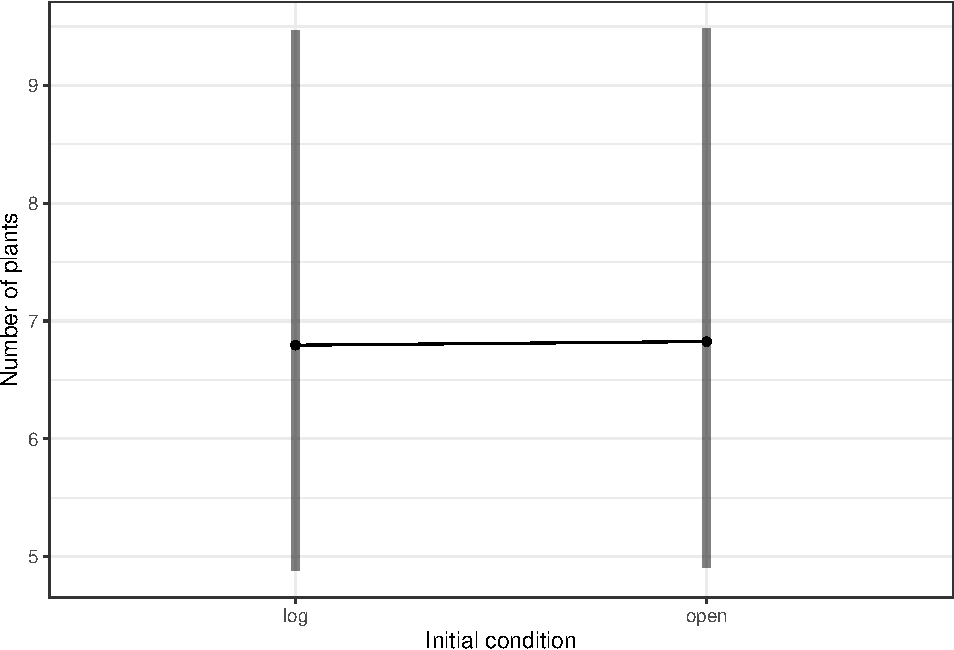
\includegraphics{log-project-aubrie-winnie_files/figure-latex/unnamed-chunk-1-1.pdf}

\hypertarget{diversity-analysis}{%
\subparagraph{Diversity analysis}\label{diversity-analysis}}

\begin{Shaded}
\begin{Highlighting}[]
\FunctionTok{require}\NormalTok{(vegan)}
\FunctionTok{require}\NormalTok{(dplyr)}
\FunctionTok{require}\NormalTok{(tidyr)}
\FunctionTok{require}\NormalTok{(labdsv)}
\FunctionTok{require}\NormalTok{(stringr)}
\FunctionTok{require}\NormalTok{(ggplot2)}
\FunctionTok{require}\NormalTok{(ggrepel)}
\FunctionTok{require}\NormalTok{(lme4)}
\FunctionTok{require}\NormalTok{(emmeans)}
\FunctionTok{require}\NormalTok{(lmerTest)}
\end{Highlighting}
\end{Shaded}

\begin{verbatim}
## Loading required package: lmerTest
\end{verbatim}

\begin{verbatim}
## 
## Attaching package: 'lmerTest'
\end{verbatim}

\begin{verbatim}
## The following object is masked from 'package:lme4':
## 
##     lmer
\end{verbatim}

\begin{verbatim}
## The following object is masked from 'package:stats':
## 
##     step
\end{verbatim}

\begin{Shaded}
\begin{Highlighting}[]
\FunctionTok{require}\NormalTok{(performance)}
\end{Highlighting}
\end{Shaded}

\begin{verbatim}
## Loading required package: performance
\end{verbatim}

\begin{Shaded}
\begin{Highlighting}[]
\FunctionTok{require}\NormalTok{(ggpubr)}
\FunctionTok{require}\NormalTok{(DHARMa)}
\end{Highlighting}
\end{Shaded}

\begin{verbatim}
## Loading required package: DHARMa
\end{verbatim}

\begin{verbatim}
## This is DHARMa 0.4.6. For overview type '?DHARMa'. For recent changes, type news(package = 'DHARMa')
\end{verbatim}

\begin{Shaded}
\begin{Highlighting}[]
\FunctionTok{require}\NormalTok{(patchwork)}
\end{Highlighting}
\end{Shaded}

\begin{verbatim}
## Loading required package: patchwork
\end{verbatim}

\begin{Shaded}
\begin{Highlighting}[]
\CommentTok{\# This dataset does not include data where the plant identity is unknown.}
\NormalTok{comm }\OtherTok{\textless{}{-}} \FunctionTok{read.csv}\NormalTok{(}\StringTok{"20{-}22\_species\_composition\_data\_no\_unk.csv"}\NormalTok{, }\AttributeTok{header =}\NormalTok{ T)}

\CommentTok{\# Remove the locations surveyed in 2021 and 2022 that were not surveyed in 2020 {-} aka, cm=0, cm=21, cm = 22, cm = 29.}
\NormalTok{comm}\OtherTok{\textless{}{-}}\NormalTok{comm[}\FunctionTok{which}\NormalTok{(comm}\SpecialCharTok{$}\NormalTok{cm\_location}\SpecialCharTok{!=}\DecValTok{21} \SpecialCharTok{\&}\NormalTok{ comm}\SpecialCharTok{$}\NormalTok{cm\_location}\SpecialCharTok{!=}\DecValTok{0} \SpecialCharTok{\&}\NormalTok{ comm}\SpecialCharTok{$}\NormalTok{cm\_location}\SpecialCharTok{!=}\DecValTok{22} \SpecialCharTok{\&}\NormalTok{ comm}\SpecialCharTok{$}\NormalTok{cm\_location}\SpecialCharTok{!=}\DecValTok{29}\NormalTok{),]}

\CommentTok{\# make a group name for each row}
\NormalTok{comm}\SpecialCharTok{$}\NormalTok{grp}\OtherTok{\textless{}{-}}\FunctionTok{apply}\NormalTok{(comm[}\FunctionTok{c}\NormalTok{(}\DecValTok{1}\NormalTok{,}\DecValTok{3}\NormalTok{,}\DecValTok{5}\NormalTok{,}\DecValTok{6}\NormalTok{,}\DecValTok{7}\NormalTok{)], }\DecValTok{1}\NormalTok{, paste, }\AttributeTok{collapse=}\StringTok{":"}\NormalTok{) }\CommentTok{\# timepoint, block, transect\_name, initial state}

\CommentTok{\# Need to make each row a community using matrify}
\NormalTok{commsub}\OtherTok{\textless{}{-}}\NormalTok{comm[,}\FunctionTok{c}\NormalTok{(}\DecValTok{15}\NormalTok{,}\DecValTok{10}\NormalTok{,}\DecValTok{13}\NormalTok{)] }

\CommentTok{\# group, species\_code, and count of each species for each transect. transects are rows.}
\NormalTok{commsub }\OtherTok{\textless{}{-}}\FunctionTok{as.data.frame}\NormalTok{(commsub)}
\NormalTok{commtry}\OtherTok{\textless{}{-}}\NormalTok{labdsv}\SpecialCharTok{::}\FunctionTok{matrify}\NormalTok{(commsub) }\CommentTok{\# make it an expanded species matrix }
\end{Highlighting}
\end{Shaded}

\begin{verbatim}
## Warning in labdsv::matrify(commsub): NAs introduced by coercion
\end{verbatim}

\begin{Shaded}
\begin{Highlighting}[]
\NormalTok{commtry}\SpecialCharTok{$}\NormalTok{x[}\FunctionTok{which}\NormalTok{(}\FunctionTok{is.na}\NormalTok{(commtry}\SpecialCharTok{$}\NormalTok{x))] }\OtherTok{\textless{}{-}} \DecValTok{1}  \CommentTok{\# "x" means that there were no individuals in the transect, but we are going to keep track of this as if it were a species}
\CommentTok{\# ncol(commtry) \# how many species are we working with in our community matrix}

\CommentTok{\# Store grouping row names as a column, then remove rownames.}
\NormalTok{commtry}\SpecialCharTok{$}\NormalTok{grps}\OtherTok{\textless{}{-}}\FunctionTok{rownames}\NormalTok{(commtry)}
\FunctionTok{rownames}\NormalTok{(commtry)}\OtherTok{\textless{}{-}}\ConstantTok{NULL}
\CommentTok{\# names(commtry)}

\CommentTok{\# Split group info into columns for each variable}
\NormalTok{mat}\OtherTok{\textless{}{-}}\FunctionTok{separate}\NormalTok{(commtry, }\DecValTok{88}\NormalTok{, }\FunctionTok{c}\NormalTok{(}\StringTok{"time"}\NormalTok{,}\StringTok{"block"}\NormalTok{,}\StringTok{"transect"}\NormalTok{,}\StringTok{"init"}\NormalTok{,}\StringTok{"treatment"}\NormalTok{), }\StringTok{":"}\NormalTok{)}
\CommentTok{\# names(mat) \#check}

\CommentTok{\# Add groupname using time, block, init columns}
\NormalTok{mat}\SpecialCharTok{$}\NormalTok{grp}\OtherTok{\textless{}{-}}\FunctionTok{apply}\NormalTok{(mat[}\FunctionTok{c}\NormalTok{(}\DecValTok{88}\SpecialCharTok{:}\DecValTok{92}\NormalTok{)], }\DecValTok{1}\NormalTok{, paste, }\AttributeTok{collapse=}\StringTok{":"}\NormalTok{)}
\CommentTok{\# ynames(mat) \#check}

\CommentTok{\# Another df where the grouping variables are time, block, transect and initial state.}
\CommentTok{\# Each row is a transect in a certain year.}
\NormalTok{df}\OtherTok{\textless{}{-}}\NormalTok{mat[,}\FunctionTok{c}\NormalTok{(}\DecValTok{1}\SpecialCharTok{:}\DecValTok{87}\NormalTok{,}\DecValTok{93}\NormalTok{)]}
\NormalTok{df2 }\OtherTok{=}\NormalTok{ df }\SpecialCharTok{\%\textgreater{}\%} \FunctionTok{mutate}\NormalTok{(}\FunctionTok{across}\NormalTok{(}\AttributeTok{.cols=}\DecValTok{1}\SpecialCharTok{:}\DecValTok{87}\NormalTok{,}\AttributeTok{.fns=}\NormalTok{as.numeric)) }\CommentTok{\# make everything numeric}
\FunctionTok{rownames}\NormalTok{(df2)}\OtherTok{\textless{}{-}}\ConstantTok{NULL} \CommentTok{\# remove rownames}

\DocumentationTok{\#\#\#\#\#\# Species diversity analysis for 2020 {-} 2022 data (Shannon diversity on transect level) }
\NormalTok{numat }\OtherTok{=}\NormalTok{ mat }\SpecialCharTok{\%\textgreater{}\%} \FunctionTok{mutate}\NormalTok{(}\FunctionTok{across}\NormalTok{(}\AttributeTok{.cols=}\DecValTok{1}\SpecialCharTok{:}\DecValTok{87}\NormalTok{,}\AttributeTok{.fns=}\NormalTok{as.numeric)) }\CommentTok{\# make everything numeric}

\CommentTok{\# sum species for each group (grouped by init, transect, block, time)}
\NormalTok{nudat}\OtherTok{\textless{}{-}}\NormalTok{numat}\SpecialCharTok{\%\textgreater{}\%} 
  \FunctionTok{group\_by}\NormalTok{(time, block, transect, init, treatment) }\SpecialCharTok{\%\textgreater{}\%} \FunctionTok{summarise}\NormalTok{(}\FunctionTok{across}\NormalTok{(}\FunctionTok{where}\NormalTok{(is.numeric), sum))}
\end{Highlighting}
\end{Shaded}

\begin{verbatim}
## `summarise()` has grouped output by 'time', 'block', 'transect', 'init'. You
## can override using the `.groups` argument.
\end{verbatim}

\begin{Shaded}
\begin{Highlighting}[]
\CommentTok{\# make a data frame}
\NormalTok{dat}\OtherTok{\textless{}{-}}\FunctionTok{as.data.frame}\NormalTok{(nudat) }\CommentTok{\# this df contains transect levels from all years}
\NormalTok{dat}\OtherTok{\textless{}{-}}\NormalTok{dat[}\FunctionTok{which}\NormalTok{(dat}\SpecialCharTok{$}\NormalTok{time}\SpecialCharTok{==}\StringTok{"t0"} \SpecialCharTok{|}\NormalTok{  dat}\SpecialCharTok{$}\NormalTok{treatment}\SpecialCharTok{==}\StringTok{"open"} \SpecialCharTok{|}\NormalTok{  dat}\SpecialCharTok{$}\NormalTok{treatment}\SpecialCharTok{==}\StringTok{"insitu\_log"}\NormalTok{),]}

\CommentTok{\#estimate diversity for each row/group. don\textquotesingle{}t include \textquotesingle{}x\textquotesingle{} }

\CommentTok{\# no groups, just estimate diversity of each row}
\NormalTok{est}\OtherTok{\textless{}{-}}\NormalTok{dat[,}\FunctionTok{c}\NormalTok{(}\DecValTok{6}\SpecialCharTok{:}\DecValTok{91}\NormalTok{)]}
\NormalTok{dat}\SpecialCharTok{$}\NormalTok{diversity}\OtherTok{\textless{}{-}}\FunctionTok{diversity}\NormalTok{(est, }\AttributeTok{index=}\StringTok{\textquotesingle{}shannon\textquotesingle{}}\NormalTok{) }

\DocumentationTok{\#\#\#\#\#\# We used a hurdle model since the data is zero{-}inflated}
\CommentTok{\# separate into zero and non{-}zero observations}
\NormalTok{dat}\SpecialCharTok{$}\NormalTok{non\_zero }\OtherTok{\textless{}{-}} \FunctionTok{ifelse}\NormalTok{(dat}\SpecialCharTok{$}\NormalTok{diversity }\SpecialCharTok{\textgreater{}} \DecValTok{0}\NormalTok{, }\DecValTok{1}\NormalTok{, }\DecValTok{0}\NormalTok{)}

\CommentTok{\# what does our data look like? }
\CommentTok{\# hist(dat$diversity, xlab = "Shannon diversity", main = "Histogram of Shannon diversity index (all years, transect level)") \# zero{-}inflated}

\CommentTok{\# ggplot(dat, aes(x = diversity, fill = as.factor(non\_zero))) +}
\CommentTok{\#  geom\_histogram(position = "identity", alpha = 1, bins = 30) +}
\CommentTok{\#  labs(x = "Diversity",}
\CommentTok{\#       y = "Frequency") +}
\CommentTok{\#  scale\_fill\_discrete(name = \textquotesingle{}non\_zero\textquotesingle{}) +}
\CommentTok{\#  theme\_bw()}

\CommentTok{\# shapiro.test((dat$diversity[dat$non\_zero == 1])) \# non{-}zero data is not normal}

\CommentTok{\# Non{-}zero data is, however, an approximate Gaussian distribution}
\CommentTok{\# hist(dat$diversity[dat$non\_zero ==1], xlab = "Shannon diversity index (non{-}zero)", main = "Histogram of Shannon diversity index (non{-}zero, all years, transect level)") \# visually it resembles a lot like a Gaussian distribution }

\CommentTok{\# Gaussian distribution produced the best{-}fitting ggplot}
\CommentTok{\# dat\_nonzerodat \textless{}{-} dat[dat$non\_zero == 1, ]}
\CommentTok{\# ggplot(dat\_nonzerodat, aes(sample = diversity)) + }
\CommentTok{\#                   geom\_qq(distribution = qnorm) + }
\CommentTok{\#                  geom\_qq\_line(distribution = qnorm) +}
\CommentTok{\#                  ggtitle("normal")}

\CommentTok{\# Hurdle model part 1. Logistic regression to predict the probability of non{-}zero.}
\CommentTok{\# Ppen and log environment does determine the probability of non{-}zero diversity index}
\CommentTok{\# 0 Shannon diversity index =/= zero plants}
\NormalTok{Hurd.mod}\FloatTok{.1} \OtherTok{\textless{}{-}} \FunctionTok{glmer}\NormalTok{(non\_zero }\SpecialCharTok{\textasciitilde{}}\NormalTok{ init }\SpecialCharTok{+}\NormalTok{ (}\DecValTok{1}\SpecialCharTok{|}\NormalTok{block) }\SpecialCharTok{+}\NormalTok{ (}\DecValTok{1}\SpecialCharTok{|}\NormalTok{time), }\AttributeTok{data =}\NormalTok{ dat, }\AttributeTok{family =}\NormalTok{ binomial)}
\CommentTok{\# summary(Hurd.mod.1) \# significant}

\CommentTok{\# Hurdle model part 1. Linear mixed effect model to predict the mean of the non{-}zero data.}
\CommentTok{\# We included block and time as random terms.}
\CommentTok{\# Open and log environment is significant in explaining the plant diversity in transect levels.}
\CommentTok{\# Lmer was used because the distribution of non{-}zero data is approximally normal.}
\NormalTok{Hurd.mod}\FloatTok{.2} \OtherTok{\textless{}{-}} \FunctionTok{lmer}\NormalTok{(diversity }\SpecialCharTok{\textasciitilde{}}\NormalTok{ init }\SpecialCharTok{+}\NormalTok{ (}\DecValTok{1}\SpecialCharTok{|}\NormalTok{block)}\SpecialCharTok{+}\NormalTok{ (}\DecValTok{1}\SpecialCharTok{|}\NormalTok{time), }\AttributeTok{data=}\FunctionTok{subset}\NormalTok{(dat, non\_zero }\SpecialCharTok{==} \DecValTok{1}\NormalTok{))}
\CommentTok{\# summary(Hurd.mod.2)}
\CommentTok{\# anova(Hurd.mod.2) \# lmer on non{-}zero diversity values is significant}

\FunctionTok{tab\_model}\NormalTok{(Hurd.mod}\FloatTok{.1}\NormalTok{, Hurd.mod}\FloatTok{.2}\NormalTok{, }\AttributeTok{dv.labels=}\FunctionTok{c}\NormalTok{(}\StringTok{"Prob. SDI\textgreater{}0"}\NormalTok{, }\StringTok{"Pron. when SDI\textgreater{}0"}\NormalTok{), }\AttributeTok{title =} \StringTok{"Shannon diversity index (SDI): 2020{-}2022"}\NormalTok{, }\AttributeTok{file =} \StringTok{"sdi\_openlog\_allyear.html"}\NormalTok{)}
\end{Highlighting}
\end{Shaded}

Shannon diversity index (SDI): 2020-2022

~

Prob. SDI\textgreater0

Pron. when SDI\textgreater0

Predictors

Odds Ratios

CI

p

Estimates

CI

p

(Intercept)

9.43

3.74~--~23.77

\textless0.001

1.08

0.98~--~1.17

\textless0.001

init {[}open{]}

0.55

0.32~--~0.94

0.030

-0.09

-0.17~--~-0.02

0.019

Random Effects

σ2

3.29

0.12

τ00

0.12 block

0.00 block

0.40 time

0.00 time

ICC

0.13

0.04

N

7 block

7 block

3 time

3 time

Observations

393

319

Marginal R2 / Conditional R2

0.023 / 0.155

0.017 / 0.059

\begin{Shaded}
\begin{Highlighting}[]
\NormalTok{htmltools}\SpecialCharTok{::}\FunctionTok{includeHTML}\NormalTok{(}\StringTok{"sdi\_openlog\_allyear.html"}\NormalTok{)}
\end{Highlighting}
\end{Shaded}

\begin{Shaded}
\begin{Highlighting}[]
\CommentTok{\# Check residual}
\CommentTok{\# residuals \textless{}{-} resid(Hurd.mod.2) \# Extract residuals}
\CommentTok{\# plot(residuals)}
\CommentTok{\# abline(0,0)}
\CommentTok{\# check\_model(Hurd.mod.2)}

\DocumentationTok{\#\#\#\#\#\# Species diversity analysis for 2020 data (Shannon diversity on transect level) }
\NormalTok{dat}\SpecialCharTok{$}\NormalTok{non\_zero }\OtherTok{\textless{}{-}} \FunctionTok{ifelse}\NormalTok{(dat}\SpecialCharTok{$}\NormalTok{diversity }\SpecialCharTok{\textgreater{}} \DecValTok{0}\NormalTok{, }\DecValTok{1}\NormalTok{, }\DecValTok{0}\NormalTok{)}
\NormalTok{dat\_2020 }\OtherTok{\textless{}{-}}\NormalTok{dat[}\FunctionTok{which}\NormalTok{(dat}\SpecialCharTok{$}\NormalTok{time}\SpecialCharTok{==}\StringTok{"t0"}\NormalTok{),] }\CommentTok{\# just t0}

\CommentTok{\# Hurdle model part 1. Logistic regression to predict the probability of non{-}zero.}
\CommentTok{\# Ppen and log environment does determine the probability of non{-}zero diversity index}
\CommentTok{\# 0 Shannon diversity index =/= zero plants}
\NormalTok{Hurd.mod}\FloatTok{.1} \OtherTok{\textless{}{-}} \FunctionTok{glmer}\NormalTok{(non\_zero }\SpecialCharTok{\textasciitilde{}}\NormalTok{ init }\SpecialCharTok{+}\NormalTok{ (}\DecValTok{1}\SpecialCharTok{|}\NormalTok{block), }\AttributeTok{data =}\NormalTok{ dat\_2020, }\AttributeTok{family =}\NormalTok{ binomial)}
\CommentTok{\# summary(Hurd.mod.1) \# significant}

\CommentTok{\# Hurdle model part 1. Linear mixed effect model to predict the mean of the non{-}zero data.}
\CommentTok{\# We included block and time as random terms.}
\CommentTok{\# Open and log environment is significant in explaining the plant diversity in transect levels.}
\CommentTok{\# Lmer was used because the distribution of non{-}zero data is approximally normal.}
\NormalTok{Hurd.mod}\FloatTok{.2} \OtherTok{\textless{}{-}} \FunctionTok{lm}\NormalTok{(diversity }\SpecialCharTok{\textasciitilde{}}\NormalTok{ init, }\AttributeTok{data=}\FunctionTok{subset}\NormalTok{(dat\_2020, non\_zero }\SpecialCharTok{==} \DecValTok{1}\NormalTok{))}
\DocumentationTok{\#\# random effect (1|block) removed since it\textquotesingle{}s close to zero}
\CommentTok{\# summary(Hurd.mod.2)}
\CommentTok{\# anova(Hurd.mod.2) \# lmer on non{-}zero diversity values is significant}

\FunctionTok{tab\_model}\NormalTok{(Hurd.mod}\FloatTok{.1}\NormalTok{, Hurd.mod}\FloatTok{.2}\NormalTok{, }\AttributeTok{dv.labels=}\FunctionTok{c}\NormalTok{(}\StringTok{"Prob. SDI\textgreater{}0"}\NormalTok{, }\StringTok{"Pron. when SDI\textgreater{}0"}\NormalTok{), }\AttributeTok{title =} \StringTok{"Shannon diversity index (SDI): 2020"}\NormalTok{, }\AttributeTok{file =} \StringTok{"sdi\_openlog\_2020.html"}\NormalTok{)}
\end{Highlighting}
\end{Shaded}

Shannon diversity index (SDI): 2020

~

Prob. SDI\textgreater0

Pron. when SDI\textgreater0

Predictors

Odds Ratios

CI

p

Estimates

CI

p

(Intercept)

3.50

2.15~--~5.72

\textless0.001

1.00

0.93~--~1.08

\textless0.001

init {[}open{]}

0.69

0.38~--~1.27

0.235

-0.08

-0.19~--~0.02

0.132

Random Effects

σ2

3.29

~

τ00

0.06 block

~

ICC

0.02

~

N

7 block

~

Observations

223

165

Marginal R2 / Conditional R2

0.010 / 0.029

0.014 / 0.008

\begin{Shaded}
\begin{Highlighting}[]
\NormalTok{htmltools}\SpecialCharTok{::}\FunctionTok{includeHTML}\NormalTok{(}\StringTok{"sdi\_openlog\_2020.html"}\NormalTok{)}
\end{Highlighting}
\end{Shaded}

\begin{Shaded}
\begin{Highlighting}[]
\CommentTok{\# Check residual}
\CommentTok{\# residuals \textless{}{-} resid(Hurd.mod.2) \# Extract residuals}
\CommentTok{\# plot(residuals, main="2020")}
\CommentTok{\# abline(0,0)}

\DocumentationTok{\#\#\#\#\#\# Species diversity analysis for 2021 data (Shannon diversity on transect level)}
\NormalTok{dat}\SpecialCharTok{$}\NormalTok{non\_zero }\OtherTok{\textless{}{-}} \FunctionTok{ifelse}\NormalTok{(dat}\SpecialCharTok{$}\NormalTok{diversity }\SpecialCharTok{\textgreater{}} \DecValTok{0}\NormalTok{, }\DecValTok{1}\NormalTok{, }\DecValTok{0}\NormalTok{)}
\NormalTok{dat\_2021 }\OtherTok{\textless{}{-}}\NormalTok{dat[}\FunctionTok{which}\NormalTok{(dat}\SpecialCharTok{$}\NormalTok{time}\SpecialCharTok{==}\StringTok{"t1"}\NormalTok{),] }\CommentTok{\# just t1}

\CommentTok{\# Hurdle model part 1. Logistic regression to predict the probability of non{-}zero.}
\CommentTok{\# Ppen and log environment does determine the probability of non{-}zero diversity index}
\CommentTok{\# 0 Shannon diversity index =/= zero plants}
\NormalTok{Hurd.mod}\FloatTok{.1} \OtherTok{\textless{}{-}} \FunctionTok{glm}\NormalTok{(non\_zero }\SpecialCharTok{\textasciitilde{}}\NormalTok{ init, }\AttributeTok{data =}\NormalTok{ dat\_2021, }\AttributeTok{family =}\NormalTok{ binomial)}
\CommentTok{\# Random effect (1|block) removed since it\textquotesingle{}s close to zero.}
\CommentTok{\# summary(Hurd.mod.1) \# significant}

\CommentTok{\# Hurdle model part 1. Linear mixed effect model to predict the mean of the non{-}zero data.}
\CommentTok{\# We included block and time as random terms.}
\CommentTok{\# Open and log environment is significant in explaining the plant diversity in transect levels.}
\CommentTok{\# Lmer was used because the distribution of non{-}zero data is approximally normal.}
\NormalTok{Hurd.mod}\FloatTok{.2} \OtherTok{\textless{}{-}} \FunctionTok{lmer}\NormalTok{(diversity }\SpecialCharTok{\textasciitilde{}}\NormalTok{ init }\SpecialCharTok{+}\NormalTok{ (}\DecValTok{1}\SpecialCharTok{|}\NormalTok{block), }\AttributeTok{data=}\FunctionTok{subset}\NormalTok{(dat\_2021, non\_zero }\SpecialCharTok{==} \DecValTok{1}\NormalTok{))}
\CommentTok{\# summary(Hurd.mod.2)}
\CommentTok{\# anova(Hurd.mod.2) \# lmer on non{-}zero diversity values is significant}

\FunctionTok{tab\_model}\NormalTok{(Hurd.mod}\FloatTok{.1}\NormalTok{, Hurd.mod}\FloatTok{.2}\NormalTok{, }\AttributeTok{dv.labels=}\FunctionTok{c}\NormalTok{(}\StringTok{"Prob. SDI\textgreater{}0"}\NormalTok{, }\StringTok{"Pron. when SDI\textgreater{}0"}\NormalTok{), }\AttributeTok{title =} \StringTok{"Shannon diversity index (SDI): 2021"}\NormalTok{, }\AttributeTok{file =} \StringTok{"sdi\_openlog\_2021.html"}\NormalTok{)}
\end{Highlighting}
\end{Shaded}

Shannon diversity index (SDI): 2021

~

Prob. SDI\textgreater0

Pron. when SDI\textgreater0

Predictors

Odds Ratios

CI

p

Estimates

CI

p

(Intercept)

29.00

6.21~--~516.79

0.001

1.06

0.93~--~1.19

\textless0.001

init {[}open{]}

0.24

0.01~--~1.45

0.194

0.00

-0.16~--~0.16

0.981

Random Effects

σ2

~

0.11

τ00

~

0.00 block

ICC

~

0.02

N

~

7 block

Observations

86

78

R2 Tjur

0.023

0.000 / 0.017

\begin{Shaded}
\begin{Highlighting}[]
\NormalTok{htmltools}\SpecialCharTok{::}\FunctionTok{includeHTML}\NormalTok{(}\StringTok{"sdi\_openlog\_2021.html"}\NormalTok{)}
\end{Highlighting}
\end{Shaded}

\begin{Shaded}
\begin{Highlighting}[]
\CommentTok{\# Check residual}
\CommentTok{\# residuals \textless{}{-} resid(Hurd.mod.2) \# Extract residuals}
\CommentTok{\# plot(residuals, main="2021")}
\CommentTok{\# abline(0,0)}

\DocumentationTok{\#\#\#\#\#\# Species diversity analysis for 2022 data (Shannon diversity on transect level) }
\NormalTok{dat}\SpecialCharTok{$}\NormalTok{non\_zero }\OtherTok{\textless{}{-}} \FunctionTok{ifelse}\NormalTok{(dat}\SpecialCharTok{$}\NormalTok{diversity }\SpecialCharTok{\textgreater{}} \DecValTok{0}\NormalTok{, }\DecValTok{1}\NormalTok{, }\DecValTok{0}\NormalTok{)}
\NormalTok{dat\_2022 }\OtherTok{\textless{}{-}}\NormalTok{dat[}\FunctionTok{which}\NormalTok{(dat}\SpecialCharTok{$}\NormalTok{time}\SpecialCharTok{==}\StringTok{"t2"}\NormalTok{),] }\CommentTok{\# just t1}

\CommentTok{\# Hurdle model part 1. Logistic regression to predict the probability of non{-}zero.}
\CommentTok{\# Ppen and log environment does determine the probability of non{-}zero diversity index}
\CommentTok{\# 0 Shannon diversity index =/= zero plants}
\NormalTok{Hurd.mod}\FloatTok{.1} \OtherTok{\textless{}{-}} \FunctionTok{glmer}\NormalTok{(non\_zero }\SpecialCharTok{\textasciitilde{}}\NormalTok{ init }\SpecialCharTok{+}\NormalTok{ (}\DecValTok{1}\SpecialCharTok{|}\NormalTok{block), }\AttributeTok{data =}\NormalTok{ dat\_2022, }\AttributeTok{family =}\NormalTok{ binomial, )}
\end{Highlighting}
\end{Shaded}

\begin{verbatim}
## Warning in checkConv(attr(opt, "derivs"), opt$par, ctrl = control$checkConv, : Model is nearly unidentifiable: large eigenvalue ratio
##  - Rescale variables?
\end{verbatim}

\begin{Shaded}
\begin{Highlighting}[]
\CommentTok{\# summary(Hurd.mod.1) \# significant}

\CommentTok{\# Hurdle model part 1. Linear mixed effect model to predict the mean of the non{-}zero data.}
\CommentTok{\# We included block and time as random terms.}
\CommentTok{\# Open and log environment is significant in explaining the plant diversity in transect levels.}
\CommentTok{\# Lmer was used because the distribution of non{-}zero data is approximally normal.}
\NormalTok{Hurd.mod}\FloatTok{.2} \OtherTok{\textless{}{-}} \FunctionTok{lmer}\NormalTok{(diversity }\SpecialCharTok{\textasciitilde{}}\NormalTok{ init }\SpecialCharTok{+}\NormalTok{ (}\DecValTok{1}\SpecialCharTok{|}\NormalTok{block), }\AttributeTok{data=}\FunctionTok{subset}\NormalTok{(dat\_2022, non\_zero }\SpecialCharTok{==} \DecValTok{1}\NormalTok{))}
\CommentTok{\# summary(Hurd.mod.2)}
\CommentTok{\# anova(Hurd.mod.2) \# lmer on non{-}zero diversity values is significant}

\FunctionTok{tab\_model}\NormalTok{(Hurd.mod}\FloatTok{.1}\NormalTok{, Hurd.mod}\FloatTok{.2}\NormalTok{, }\AttributeTok{dv.labels=}\FunctionTok{c}\NormalTok{(}\StringTok{"Prob. SDI\textgreater{}0"}\NormalTok{, }\StringTok{"Pron. when SDI\textgreater{}0"}\NormalTok{), }\AttributeTok{title =} \StringTok{"Shannon diversity index (SDI): 2022"}\NormalTok{, }\AttributeTok{file =} \StringTok{"sdi\_openlog\_2022.html"}\NormalTok{)}
\end{Highlighting}
\end{Shaded}

Shannon diversity index (SDI): 2022

~

Prob. SDI\textgreater0

Pron. when SDI\textgreater0

Predictors

Odds Ratios

CI

p

Estimates

CI

p

(Intercept)

9787243037934.08

0.00~--~Inf

0.974

1.21

1.06~--~1.36

\textless0.001

init {[}open{]}

0.00

0.00~--~Inf

0.976

-0.24

-0.41~--~-0.07

0.007

Random Effects

σ2

3.29

0.13

τ00

1.15 block

0.01 block

ICC

0.26

0.07

N

7 block

7 block

Observations

84

76

Marginal R2 / Conditional R2

0.975 / 0.981

0.088 / 0.149

\begin{Shaded}
\begin{Highlighting}[]
\NormalTok{htmltools}\SpecialCharTok{::}\FunctionTok{includeHTML}\NormalTok{(}\StringTok{"sdi\_openlog\_2022.html"}\NormalTok{)}
\end{Highlighting}
\end{Shaded}

\begin{Shaded}
\begin{Highlighting}[]
\CommentTok{\# Check residual}
\CommentTok{\# residuals \textless{}{-} resid(Hurd.mod.2) \# Extract residuals}
\CommentTok{\# plot(residuals, main="2022")}
\CommentTok{\# abline(0,0)}
\end{Highlighting}
\end{Shaded}

\hypertarget{composition-analysis}{%
\subparagraph{Composition analysis}\label{composition-analysis}}

Composition dissimilarity * 2020 *

\begin{Shaded}
\begin{Highlighting}[]
\CommentTok{\# subset data where all t0 communities, insitu log and insitu open communities at t1 and t2 are included.}
\NormalTok{mat2 }\OtherTok{\textless{}{-}}\NormalTok{ mat[}\FunctionTok{which}\NormalTok{(mat}\SpecialCharTok{$}\NormalTok{time}\SpecialCharTok{==}\StringTok{"t0"}\NormalTok{),]}
\NormalTok{mat2}\SpecialCharTok{$}\NormalTok{grp}\OtherTok{\textless{}{-}}\FunctionTok{apply}\NormalTok{(mat2[}\FunctionTok{c}\NormalTok{(}\DecValTok{89}\NormalTok{,}\DecValTok{91}\NormalTok{)], }\DecValTok{1}\NormalTok{, paste, }\AttributeTok{collapse=}\StringTok{":"}\NormalTok{) }\CommentTok{\# block, init as grouping}
\CommentTok{\# names(mat2) \#check}

\CommentTok{\# another df where the grouping variables are time, block and initial state}
\CommentTok{\# each row is a transect in a certain year.}
\NormalTok{df}\OtherTok{\textless{}{-}}\NormalTok{mat2[,}\FunctionTok{c}\NormalTok{(}\DecValTok{1}\SpecialCharTok{:}\DecValTok{87}\NormalTok{, }\DecValTok{93}\NormalTok{)]}
\NormalTok{df2 }\OtherTok{=}\NormalTok{ df }\SpecialCharTok{\%\textgreater{}\%} \FunctionTok{mutate}\NormalTok{(}\FunctionTok{across}\NormalTok{(}\AttributeTok{.cols=}\DecValTok{1}\SpecialCharTok{:}\DecValTok{87}\NormalTok{,}\AttributeTok{.fns=}\NormalTok{as.numeric)) }\CommentTok{\# make everything numeric}
\FunctionTok{rownames}\NormalTok{(df2)}\OtherTok{\textless{}{-}}\ConstantTok{NULL} \CommentTok{\# remove rownames}

\DocumentationTok{\#\# new with group vars}
\NormalTok{nublock}\OtherTok{\textless{}{-}}\FunctionTok{separate}\NormalTok{(df2, }\DecValTok{88}\NormalTok{, }\FunctionTok{c}\NormalTok{(}\StringTok{"block"}\NormalTok{, }\StringTok{"init"}\NormalTok{), }\StringTok{":"}\NormalTok{) }\CommentTok{\# just looking at time, block \& initial treatment}

\CommentTok{\# want to sum across transects in same block X init treatment}
\NormalTok{nublock}\SpecialCharTok{$}\NormalTok{sumgrp}\OtherTok{\textless{}{-}}\FunctionTok{apply}\NormalTok{(mat2[}\FunctionTok{c}\NormalTok{(}\DecValTok{89}\NormalTok{, }\DecValTok{91}\NormalTok{)], }\DecValTok{1}\NormalTok{, paste, }\AttributeTok{collapse=}\StringTok{":"}\NormalTok{)}
\CommentTok{\# head(nublock)}

\CommentTok{\# sum observations across initial X  block (group variable)}
\CommentTok{\# this gives number of plants in each transect TYPE for each year in each block. should be 2 types X 3 years X 7 blocks rows }
\NormalTok{blocksum}\OtherTok{\textless{}{-}}\FunctionTok{rowsum}\NormalTok{(nublock[,}\FunctionTok{c}\NormalTok{(}\DecValTok{1}\SpecialCharTok{:}\DecValTok{87}\NormalTok{)], }\AttributeTok{group=}\NormalTok{nublock}\SpecialCharTok{$}\NormalTok{sumgrp)}
\NormalTok{blocksum}\SpecialCharTok{$}\NormalTok{grps}\OtherTok{\textless{}{-}}\FunctionTok{rownames}\NormalTok{(blocksum)}
\FunctionTok{rownames}\NormalTok{(blocksum)}\OtherTok{\textless{}{-}}\ConstantTok{NULL} \CommentTok{\# remove rownames}
\CommentTok{\# nrow(blocksum) \# it is 14 rows as expected }

\DocumentationTok{\#\# expand again}
\NormalTok{blocksum}\OtherTok{\textless{}{-}}\FunctionTok{separate}\NormalTok{(blocksum, }\DecValTok{88}\NormalTok{, }\FunctionTok{c}\NormalTok{(}\StringTok{"block"}\NormalTok{, }\StringTok{"init"}\NormalTok{), }\StringTok{":"}\NormalTok{)}

\CommentTok{\# at the moment this includes where there were no plants ("x" column in matrix)}
\NormalTok{assemblies\_t0}\OtherTok{\textless{}{-}}\NormalTok{blocksum[,}\FunctionTok{c}\NormalTok{(}\DecValTok{1}\SpecialCharTok{:}\DecValTok{87}\NormalTok{)]}

\CommentTok{\# group {-} these are the treatment variables that need to be separately fed into the MDS analaysis from the community analysis.}
\NormalTok{group\_init}\OtherTok{\textless{}{-}}\NormalTok{blocksum}\SpecialCharTok{$}\NormalTok{init}
\NormalTok{group\_block}\OtherTok{\textless{}{-}}\NormalTok{blocksum}\SpecialCharTok{$}\NormalTok{block}

\CommentTok{\# MDS }
\NormalTok{ass.rel.t0}\OtherTok{\textless{}{-}}\FunctionTok{decostand}\NormalTok{(assemblies\_t0, }\AttributeTok{method=}\StringTok{\textquotesingle{}hel\textquotesingle{}}\NormalTok{) }\CommentTok{\#standardize assemblies }
\NormalTok{ass.rel.t0\_NMS }\OtherTok{\textless{}{-}} \FunctionTok{metaMDS}\NormalTok{(ass.rel.t0, }\AttributeTok{distance =} \StringTok{\textquotesingle{}bray\textquotesingle{}}\NormalTok{, }\AttributeTok{k =} \DecValTok{4}\NormalTok{) }\CommentTok{\# run MDS }
\end{Highlighting}
\end{Shaded}

\begin{verbatim}
## Run 0 stress 0.04866056 
## Run 1 stress 0.04798369 
## ... New best solution
## ... Procrustes: rmse 0.1312496  max resid 0.3125486 
## Run 2 stress 0.04866065 
## Run 3 stress 0.04866055 
## Run 4 stress 0.04866031 
## Run 5 stress 0.04866069 
## Run 6 stress 0.04866041 
## Run 7 stress 0.04866052 
## Run 8 stress 0.04866012 
## Run 9 stress 0.05072948 
## Run 10 stress 0.05156182 
## Run 11 stress 0.04798374 
## ... Procrustes: rmse 0.0002619949  max resid 0.0006066103 
## ... Similar to previous best
## Run 12 stress 0.04866058 
## Run 13 stress 0.05073228 
## Run 14 stress 0.04866061 
## Run 15 stress 0.05215832 
## Run 16 stress 0.04798376 
## ... Procrustes: rmse 9.207454e-05  max resid 0.0001601271 
## ... Similar to previous best
## Run 17 stress 0.04866022 
## Run 18 stress 0.04866032 
## Run 19 stress 0.04798377 
## ... Procrustes: rmse 0.0001144348  max resid 0.0002943744 
## ... Similar to previous best
## Run 20 stress 0.0486606 
## *** Best solution repeated 3 times
\end{verbatim}

\begin{Shaded}
\begin{Highlighting}[]
\CommentTok{\# stressplot(ass.rel.t0\_NMS) \# check fit}

\CommentTok{\# scores}
\NormalTok{mds\_scores\_t0}\OtherTok{\textless{}{-}}\FunctionTok{as.data.frame}\NormalTok{(vegan}\SpecialCharTok{::}\FunctionTok{scores}\NormalTok{(ass.rel.t0\_NMS)}\SpecialCharTok{$}\NormalTok{sites) }\CommentTok{\# extract scores}
\NormalTok{mds\_scores\_t0}\SpecialCharTok{$}\NormalTok{site}\OtherTok{\textless{}{-}}\FunctionTok{rownames}\NormalTok{(vegan}\SpecialCharTok{::}\FunctionTok{scores}\NormalTok{(ass.rel.t0\_NMS)}\SpecialCharTok{$}\NormalTok{sites) }\CommentTok{\# extract names }
\NormalTok{mds\_scores\_t0}\SpecialCharTok{$}\NormalTok{treatment}\OtherTok{\textless{}{-}}\NormalTok{group\_init }\CommentTok{\# grouping factor 1 }
\NormalTok{mds\_scores\_t0}\SpecialCharTok{$}\NormalTok{block}\OtherTok{\textless{}{-}}\NormalTok{group\_block }\CommentTok{\# grouping factor 2 }

\CommentTok{\# explaining factors}
\NormalTok{init}\OtherTok{\textless{}{-}}\FunctionTok{as.factor}\NormalTok{(group\_init) }\CommentTok{\# grouping factor 1{-} convert to factor}
\NormalTok{block}\OtherTok{\textless{}{-}}\FunctionTok{as.factor}\NormalTok{(group\_block) }\CommentTok{\# grouping factor 2{-} convert to factor}

\DocumentationTok{\#\#\#\# Redundancy analysis}
\CommentTok{\# can look at significance of model where initial treatment and block explain variation in community}
\CommentTok{\# trt\_tot\_2\textless{}{-}rda(ass.rel.t0\textasciitilde{}init+block) \# run model using standardized data }
\CommentTok{\# summary(trt\_tot\_2)}
\CommentTok{\# anova.cca(trt\_tot\_2, step=1000, by="term") \#\# test for model significance}

\CommentTok{\# Using varpart to look at contributions of initial treatment and block}
\NormalTok{var.mod2}\OtherTok{\textless{}{-}}\FunctionTok{varpart}\NormalTok{(ass.rel.t0, init, block) }\CommentTok{\# run model on standardized data}
\FunctionTok{plot}\NormalTok{(var.mod2, }\AttributeTok{bg=}\FunctionTok{c}\NormalTok{(}\StringTok{"hotpink"}\NormalTok{,}\StringTok{"skyblue"}\NormalTok{))}
\FunctionTok{mtext}\NormalTok{(}\StringTok{"X1= Treatment; X2=Block"}\NormalTok{, }\AttributeTok{side=}\DecValTok{3}\NormalTok{)}
\end{Highlighting}
\end{Shaded}

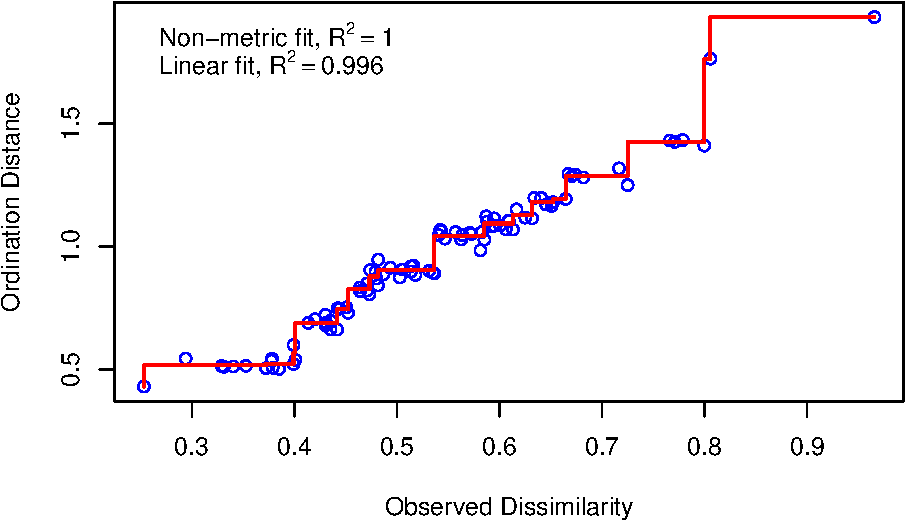
\includegraphics{log-project-aubrie-winnie_files/figure-latex/unnamed-chunk-4-1.pdf}

\begin{Shaded}
\begin{Highlighting}[]
\CommentTok{\# can test for significance of contribution of the fraction of initial treatment}
\CommentTok{\# do this with partial redundancy analysis}
\NormalTok{trt\_Frac}\OtherTok{\textless{}{-}}\FunctionTok{rda}\NormalTok{(ass.rel.t0, init, block) }\CommentTok{\# partial rda model}
\FunctionTok{summary}\NormalTok{(trt\_Frac)}
\end{Highlighting}
\end{Shaded}

\begin{verbatim}
## 
## Call:
## rda(X = ass.rel.t0, Y = init, Z = block) 
## 
## Partitioning of variance:
##               Inertia Proportion
## Total         0.42624    1.00000
## Conditioned   0.29429    0.69045
## Constrained   0.03551    0.08332
## Unconstrained 0.09643    0.22624
## 
## Eigenvalues, and their contribution to the variance 
## after removing the contribution of conditiniong variables
## 
## Importance of components:
##                          RDA1     PC1     PC2     PC3     PC4     PC5      PC6
## Eigenvalue            0.03551 0.03207 0.02047 0.01524 0.01394 0.01034 0.004375
## Proportion Explained  0.26916 0.24303 0.15511 0.11552 0.10566 0.07837 0.033159
## Cumulative Proportion 0.26916 0.51219 0.66730 0.78282 0.88848 0.96684 1.000000
## 
## Accumulated constrained eigenvalues
## Importance of components:
##                          RDA1
## Eigenvalue            0.03551
## Proportion Explained  1.00000
## Cumulative Proportion 1.00000
## 
## Scaling 2 for species and site scores
## * Species are scaled proportional to eigenvalues
## * Sites are unscaled: weighted dispersion equal on all dimensions
## * General scaling constant of scores:  1.534259 
## 
## 
## Species scores
## 
##             RDA1        PC1        PC2        PC3        PC4        PC5
## acul   0.1067309 -9.564e-02 -2.516e-02  6.791e-02 -5.735e-02 -1.985e-02
## aicu   0.0342552  7.579e-02 -2.904e-02 -1.040e-01 -1.656e-02  3.629e-04
## arca   0.0000000 -5.092e-17  4.573e-17 -2.095e-17  2.733e-18  2.352e-18
## ardy   0.0000000 -1.340e-17  2.878e-18  4.804e-18  6.089e-18  3.913e-18
## arsp   0.0212814 -9.296e-03  3.074e-02 -1.243e-02  2.902e-02  2.380e-02
## auel   0.0000000  1.657e-17  1.767e-18 -7.370e-18 -1.235e-17 -4.376e-19
## bldr   0.0627812 -3.489e-02  5.885e-02 -3.487e-02  5.598e-02 -1.193e-01
## blrd   0.0000000  2.296e-18  1.300e-17  5.184e-19  1.453e-17  5.429e-18
## brdi   0.0000000 -1.645e-17  1.224e-17 -1.804e-17 -5.031e-18  1.778e-17
## brdr   0.0000000 -1.535e-18  1.057e-18  1.817e-19  3.219e-18  1.290e-18
## brpe   0.0000000  4.493e-17  7.212e-18 -2.652e-17 -7.924e-17 -1.269e-17
## brru   0.0000000 -3.497e-33 -2.348e-33  3.058e-33  5.468e-33 -1.861e-34
## buse  -0.0399181  8.064e-03 -8.920e-03 -7.638e-03 -1.217e-02  6.087e-02
## caer  -0.0770469  5.739e-03 -4.007e-02  2.232e-02 -3.681e-02  4.977e-02
## cagr  -0.0353354  3.492e-02 -5.082e-02 -7.084e-02  2.218e-02  4.523e-02
## cahi   0.0073560  1.491e-02  4.828e-02 -6.274e-03  3.863e-02  1.972e-02
## casp   0.0071091 -7.320e-02 -4.968e-02  8.494e-03  2.080e-02  8.123e-03
## cear   0.0000000  0.000e+00  0.000e+00  0.000e+00  0.000e+00  0.000e+00
## chau   0.0270050  2.642e-02  5.365e-02 -7.004e-02 -9.242e-02 -2.682e-03
## chei   0.0000000  0.000e+00  0.000e+00  0.000e+00  0.000e+00  0.000e+00
## chps   0.0867979 -8.706e-02 -4.807e-02  5.256e-03 -3.053e-02 -5.813e-02
## crcl   0.0000000  0.000e+00  0.000e+00  0.000e+00  0.000e+00  0.000e+00
## crco  -0.0054567 -2.817e-02 -2.789e-02 -6.578e-02 -6.492e-03  6.700e-02
## cusc   0.0000000  0.000e+00  0.000e+00  0.000e+00  0.000e+00  0.000e+00
## cusp   0.0000000  0.000e+00  0.000e+00  0.000e+00  0.000e+00  0.000e+00
## dagl  -0.0005158 -4.170e-02 -1.197e-02  1.578e-02 -3.486e-02  3.748e-02
## dosp   0.0000000  0.000e+00  0.000e+00  0.000e+00  0.000e+00  0.000e+00
## ento   0.0000000  0.000e+00  0.000e+00  0.000e+00  0.000e+00  0.000e+00
## erau   0.0000000  0.000e+00  0.000e+00  0.000e+00  0.000e+00  0.000e+00
## ercy   0.0000000  0.000e+00  0.000e+00  0.000e+00  0.000e+00  0.000e+00
## erra  -0.0017634  1.363e-03 -1.961e-03 -2.641e-03  6.378e-04  2.340e-03
## ersp  -0.0209707  1.621e-02 -2.332e-02 -3.140e-02  7.584e-03  2.783e-02
## gite  -0.0057450 -7.634e-03  5.428e-03 -7.119e-03 -3.080e-03 -1.608e-03
## gnte   0.0000000  0.000e+00  0.000e+00  0.000e+00  0.000e+00  0.000e+00
## gobe  -0.0320039 -3.133e-03 -9.076e-02  5.077e-02  1.243e-01  2.247e-02
## gocy  -0.0012808  6.463e-02  4.761e-02 -1.112e-02 -1.947e-02 -4.368e-03
## gono   0.0000000  0.000e+00  0.000e+00  0.000e+00  0.000e+00  0.000e+00
## goro   0.0215820  2.211e-01 -1.082e-01 -1.141e-02 -4.094e-02 -1.836e-02
## gosp   0.0446889  2.138e-02  1.224e-02  1.185e-02  3.669e-02  2.988e-02
## haod  -0.0050284 -3.182e-02  7.735e-03  1.165e-02  6.116e-02  1.742e-02
## hygl   0.0601486  6.535e-02  7.287e-02  6.640e-02 -5.544e-02  7.196e-02
## hypi   0.0000000  0.000e+00  0.000e+00  0.000e+00  0.000e+00  0.000e+00
## hypo   0.0000000  0.000e+00  0.000e+00  0.000e+00  0.000e+00  0.000e+00
## jubu   0.0000000  0.000e+00  0.000e+00  0.000e+00  0.000e+00  0.000e+00
## laro  -0.1146604 -4.765e-02 -1.202e-02  3.910e-02 -4.021e-02 -1.545e-02
## ledu   0.0000000  0.000e+00  0.000e+00  0.000e+00  0.000e+00  0.000e+00
## lele   0.0212814 -9.296e-03  3.074e-02 -1.243e-02  2.902e-02  2.380e-02
## loef   0.0000000  0.000e+00  0.000e+00  0.000e+00  0.000e+00  0.000e+00
## misp  -0.0859180  4.494e-02 -1.140e-01 -3.971e-02 -2.276e-02  5.166e-03
## mite   0.0000000  0.000e+00  0.000e+00  0.000e+00  0.000e+00  0.000e+00
## momo   0.0000000  0.000e+00  0.000e+00  0.000e+00  0.000e+00  0.000e+00
## mopa   0.0000000  0.000e+00  0.000e+00  0.000e+00  0.000e+00  0.000e+00
## niro   0.0000000  0.000e+00  0.000e+00  0.000e+00  0.000e+00  0.000e+00
## omco   0.0102406 -1.780e-02 -1.290e-02 -4.528e-03 -7.063e-03  3.001e-03
## orsp   0.0000000  0.000e+00  0.000e+00  0.000e+00  0.000e+00  0.000e+00
## pala   0.0212814 -9.296e-03  3.074e-02 -1.243e-02  2.902e-02  2.380e-02
## peai   0.0697049  5.909e-02 -2.821e-03  5.278e-02 -3.971e-02 -2.331e-02
## pedu   0.0300964 -1.315e-02  4.347e-02 -1.758e-02  4.104e-02  3.366e-02
## phsu   0.0000000  0.000e+00  0.000e+00  0.000e+00  0.000e+00  0.000e+00
## plde   0.0000000  0.000e+00  0.000e+00  0.000e+00  0.000e+00  0.000e+00
## poar   0.0000000  0.000e+00  0.000e+00  0.000e+00  0.000e+00  0.000e+00
## poca   0.0311535  7.429e-02  1.806e-02  8.779e-02  2.715e-02 -2.008e-02
## pocap  0.0157620  1.774e-02  1.191e-02 -1.551e-02 -2.774e-02  9.443e-04
## poce   0.0000000  0.000e+00  0.000e+00  0.000e+00  0.000e+00  0.000e+00
## pogn   0.0000000  0.000e+00  0.000e+00  0.000e+00  0.000e+00  0.000e+00
## pole  -0.0067798  6.543e-02  2.974e-02  8.404e-02 -4.950e-03 -2.006e-02
## pomu   0.1806915 -8.052e-02 -1.066e-01  1.495e-02 -1.385e-02 -5.198e-02
## pter   0.0000000  0.000e+00  0.000e+00  0.000e+00  0.000e+00  0.000e+00
## ptga  -0.0265218  3.413e-02  8.198e-05  2.118e-02  4.241e-02  3.353e-02
## ptob   0.0000000  0.000e+00  0.000e+00  0.000e+00  0.000e+00  0.000e+00
## rhla   0.0114587  1.612e-02 -1.907e-02  1.253e-01 -6.133e-02  3.825e-02
## rhpy  -0.0614885  1.909e-01  1.451e-02  3.551e-03  8.057e-02 -4.550e-02
## rhsp   0.0000000  0.000e+00  0.000e+00  0.000e+00  0.000e+00  0.000e+00
## ry     0.0000000  0.000e+00  0.000e+00  0.000e+00  0.000e+00  0.000e+00
## scna   0.0000000  0.000e+00  0.000e+00  0.000e+00  0.000e+00  0.000e+00
## sino   0.0000000  0.000e+00  0.000e+00  0.000e+00  0.000e+00  0.000e+00
## sool   0.0000000  0.000e+00  0.000e+00  0.000e+00  0.000e+00  0.000e+00
## stfi  -0.0217745 -2.451e-02 -1.645e-02  2.143e-02  3.832e-02 -1.304e-03
## stpi   0.0000000  0.000e+00  0.000e+00  0.000e+00  0.000e+00  0.000e+00
## thma   0.0000000  0.000e+00  0.000e+00  0.000e+00  0.000e+00  0.000e+00
## trcy  -0.2016923  4.678e-02  1.599e-01 -2.560e-02 -4.775e-02 -1.767e-02
## tris   0.0000000  0.000e+00  0.000e+00  0.000e+00  0.000e+00  0.000e+00
## tror  -0.1560795 -5.629e-02 -1.247e-02 -3.574e-02 -4.124e-02 -1.417e-02
## trpi  -0.0192367 -2.197e-03  9.150e-03 -9.411e-03  2.883e-03 -2.219e-02
## waac  -0.1168716 -1.021e-01  4.820e-02 -2.229e-02  7.287e-04 -5.756e-03
## wagr  -0.0763637  1.108e-02 -5.682e-02 -5.042e-02 -3.786e-02  2.435e-03
## x     -0.0563652 -6.808e-02  4.036e-02 -1.343e-02  3.574e-02  6.019e-02
## 
## 
## Site scores (weighted sums of species scores)
## 
##          RDA1      PC1     PC2     PC3      PC4      PC5
## sit1  -0.4306 -0.15560  0.2593  0.4984 -0.43518  0.64698
## sit2   0.4306  0.15560 -0.2593 -0.4984  0.43518 -0.64698
## sit3  -0.5088 -0.54489  0.3874 -0.5081 -0.21987 -0.11475
## sit4   0.5088  0.54489 -0.3874  0.5081  0.21987  0.11475
## sit5  -0.3922 -0.04684  0.1950 -0.2006  0.06145 -0.47310
## sit6   0.3922  0.04684 -0.1950  0.2006 -0.06145  0.47310
## sit7  -0.5074  0.31689 -0.4561 -0.6141  0.14830  0.54414
## sit8   0.5074 -0.31689  0.4561  0.6141 -0.14830 -0.54414
## sit9  -0.5125  0.71285  0.5165  0.1813  0.28281 -0.12016
## sit10  0.5125 -0.71285 -0.5165 -0.1813 -0.28281  0.12016
## sit11 -0.2572  0.17912 -0.5923  0.2395 -0.55918 -0.45854
## sit12  0.2572 -0.17912  0.5923 -0.2395  0.55918  0.45854
## sit13 -0.2616 -0.46153 -0.3099  0.4036  0.72167 -0.02456
## sit14  0.2616  0.46153  0.3099 -0.4036 -0.72167  0.02456
## 
## 
## Site constraints (linear combinations of constraining variables)
## 
##        RDA1      PC1     PC2     PC3      PC4      PC5
## con1  -0.41 -0.15560  0.2593  0.4984 -0.43518  0.64698
## con2   0.41  0.15560 -0.2593 -0.4984  0.43518 -0.64698
## con3  -0.41 -0.54489  0.3874 -0.5081 -0.21987 -0.11475
## con4   0.41  0.54489 -0.3874  0.5081  0.21987  0.11475
## con5  -0.41 -0.04684  0.1950 -0.2006  0.06145 -0.47310
## con6   0.41  0.04684 -0.1950  0.2006 -0.06145  0.47310
## con7  -0.41  0.31689 -0.4561 -0.6141  0.14830  0.54414
## con8   0.41 -0.31689  0.4561  0.6141 -0.14830 -0.54414
## con9  -0.41  0.71285  0.5165  0.1813  0.28281 -0.12016
## con10  0.41 -0.71285 -0.5165 -0.1813 -0.28281  0.12016
## con11 -0.41  0.17912 -0.5923  0.2395 -0.55918 -0.45854
## con12  0.41 -0.17912  0.5923 -0.2395  0.55918  0.45854
## con13 -0.41 -0.46153 -0.3099  0.4036  0.72167 -0.02456
## con14  0.41  0.46153  0.3099 -0.4036 -0.72167  0.02456
## 
## 
## Biplot scores for constraining variables
## 
##       RDA1 PC1 PC2 PC3 PC4 PC5
## Yopen    1   0   0   0   0   0
\end{verbatim}

\begin{Shaded}
\begin{Highlighting}[]
\FunctionTok{RsquareAdj}\NormalTok{(trt\_Frac)}\SpecialCharTok{$}\NormalTok{adj.r.squared }\CommentTok{\#explanatory power}
\end{Highlighting}
\end{Shaded}

\begin{verbatim}
## [1] 0.08471055
\end{verbatim}

\begin{Shaded}
\begin{Highlighting}[]
\FunctionTok{anova.cca}\NormalTok{(trt\_Frac) }\DocumentationTok{\#\# this tells us if first condition, init, significantly contributes to overall variance explanation. }
\end{Highlighting}
\end{Shaded}

\begin{verbatim}
## Permutation test for rda under reduced model
## Permutation: free
## Number of permutations: 999
## 
## Model: rda(X = ass.rel.t0, Y = init, Z = block)
##          Df Variance      F Pr(>F)  
## Model     1 0.035514 2.2097  0.039 *
## Residual  6 0.096430                
## ---
## Signif. codes:  0 '***' 0.001 '**' 0.01 '*' 0.05 '.' 0.1 ' ' 1
\end{verbatim}

\begin{Shaded}
\begin{Highlighting}[]
\CommentTok{\# Extracting species scores and plotting }
\CommentTok{\# Species scores}
\NormalTok{species.scores}\OtherTok{\textless{}{-}}\FunctionTok{as.data.frame}\NormalTok{(vegan}\SpecialCharTok{::}\FunctionTok{scores}\NormalTok{(ass.rel.t0\_NMS,}\StringTok{"species"}\NormalTok{)) }\DocumentationTok{\#\# some species don\textquotesingle{}t have scores}
\NormalTok{species.scores}\SpecialCharTok{$}\NormalTok{species}\OtherTok{\textless{}{-}}\FunctionTok{rownames}\NormalTok{(species.scores) }

\DocumentationTok{\#\#\# NMDS 1 and 2 }
\NormalTok{log}\OtherTok{\textless{}{-}}\NormalTok{mds\_scores\_t0[mds\_scores\_t0}\SpecialCharTok{$}\NormalTok{treatment }\SpecialCharTok{==} \StringTok{"log"}\NormalTok{, ][}\FunctionTok{chull}\NormalTok{(mds\_scores\_t0[mds\_scores\_t0}\SpecialCharTok{$}\NormalTok{treatment }\SpecialCharTok{==} 
                                                          \StringTok{"log"}\NormalTok{, }\FunctionTok{c}\NormalTok{(}\StringTok{"NMDS1"}\NormalTok{, }\StringTok{"NMDS2"}\NormalTok{)]), ]}

\NormalTok{open}\OtherTok{\textless{}{-}}\NormalTok{mds\_scores\_t0[mds\_scores\_t0}\SpecialCharTok{$}\NormalTok{treatment }\SpecialCharTok{==} \StringTok{"open"}\NormalTok{, ][}\FunctionTok{chull}\NormalTok{(mds\_scores\_t0[mds\_scores\_t0}\SpecialCharTok{$}\NormalTok{treatment }\SpecialCharTok{==} 
                                                               \StringTok{"open"}\NormalTok{, }\FunctionTok{c}\NormalTok{(}\StringTok{"NMDS1"}\NormalTok{, }\StringTok{"NMDS2"}\NormalTok{)]), ]}

\NormalTok{hulldat}\OtherTok{\textless{}{-}}\FunctionTok{rbind}\NormalTok{(log,open)}
 
\NormalTok{nmds.plot}\OtherTok{\textless{}{-}} \FunctionTok{ggplot}\NormalTok{()}\SpecialCharTok{+}
  \FunctionTok{theme\_bw}\NormalTok{()}\SpecialCharTok{+}
  \FunctionTok{theme}\NormalTok{(}\AttributeTok{panel.background =} \FunctionTok{element\_blank}\NormalTok{(),}
        \AttributeTok{panel.grid.major =} \FunctionTok{element\_blank}\NormalTok{(),  }\CommentTok{\#remove major{-}grid labels}
        \AttributeTok{panel.grid.minor =} \FunctionTok{element\_blank}\NormalTok{(),  }\CommentTok{\#remove minor{-}grid labels}
        \AttributeTok{plot.background =} \FunctionTok{element\_blank}\NormalTok{(), }
        \AttributeTok{axis.text =} \FunctionTok{element\_text}\NormalTok{(}\AttributeTok{size =} \DecValTok{15}\NormalTok{),}
        \AttributeTok{axis.title=}\FunctionTok{element\_text}\NormalTok{(}\AttributeTok{size=}\DecValTok{20}\NormalTok{),}
        \AttributeTok{legend.title=}\FunctionTok{element\_text}\NormalTok{(}\AttributeTok{size=}\DecValTok{20}\NormalTok{), }
        \AttributeTok{legend.text=}\FunctionTok{element\_text}\NormalTok{(}\AttributeTok{size=}\DecValTok{15}\NormalTok{))}\SpecialCharTok{+}
  \FunctionTok{geom\_text\_repel}\NormalTok{(}\AttributeTok{data=}\NormalTok{species.scores, }\FunctionTok{aes}\NormalTok{(NMDS1, NMDS2, }\AttributeTok{label=}\NormalTok{species), }\AttributeTok{alpha=}\FloatTok{0.9}\NormalTok{, }\AttributeTok{size=}\DecValTok{5}\NormalTok{, }\AttributeTok{col=}\StringTok{\textquotesingle{}darkgray\textquotesingle{}}\NormalTok{,}\AttributeTok{na.rm=}\ConstantTok{TRUE}\NormalTok{)}\SpecialCharTok{+}
  \FunctionTok{geom\_polygon}\NormalTok{(}\AttributeTok{data=}\NormalTok{hulldat, }\FunctionTok{aes}\NormalTok{(NMDS1, NMDS2, }\AttributeTok{fill=}\NormalTok{treatment, }\AttributeTok{group=}\NormalTok{treatment), }\AttributeTok{alpha=}\FloatTok{0.3}\NormalTok{)}\SpecialCharTok{+}\FunctionTok{scale\_fill\_manual}\NormalTok{(}\AttributeTok{values=}\FunctionTok{c}\NormalTok{(}\StringTok{"\#63A088"}\NormalTok{,}\StringTok{"\#56638A"}\NormalTok{), }\AttributeTok{name=}\StringTok{"Treatment"}\NormalTok{)}\SpecialCharTok{+}
  \FunctionTok{geom\_point}\NormalTok{(}\AttributeTok{data=}\NormalTok{mds\_scores\_t0, }\FunctionTok{aes}\NormalTok{(NMDS1, NMDS2, }\AttributeTok{shape=}\NormalTok{block, }\AttributeTok{col=}\NormalTok{treatment), }\AttributeTok{size=}\DecValTok{6}\NormalTok{)}\SpecialCharTok{+} \FunctionTok{scale\_shape\_manual}\NormalTok{(}\AttributeTok{values =} \FunctionTok{c}\NormalTok{(}\DecValTok{14}\NormalTok{,}\DecValTok{15}\NormalTok{,}\DecValTok{16}\NormalTok{,}\DecValTok{17}\NormalTok{,}\DecValTok{11}\NormalTok{,}\DecValTok{18}\NormalTok{,}\DecValTok{8}\NormalTok{), }\AttributeTok{name=}\StringTok{\textquotesingle{}Block\textquotesingle{}}\NormalTok{)}\SpecialCharTok{+}
  \FunctionTok{scale\_colour\_manual}\NormalTok{(}\AttributeTok{values=}\FunctionTok{c}\NormalTok{(}\StringTok{"\#63A088"}\NormalTok{,}\StringTok{"\#56638A"}\NormalTok{), }\AttributeTok{name=}\StringTok{"Treatment"}\NormalTok{) }\SpecialCharTok{+}
  \FunctionTok{labs}\NormalTok{(}\AttributeTok{title=}\FunctionTok{paste0}\NormalTok{(}\StringTok{"Stress: "}\NormalTok{, }\FunctionTok{round}\NormalTok{(ass.rel.t0\_NMS}\SpecialCharTok{$}\NormalTok{stress,}\DecValTok{3}\NormalTok{)))}

\CommentTok{\# print(nmds.plot)}

\CommentTok{\# All other NMDS pairs}
\NormalTok{treatments }\OtherTok{\textless{}{-}} \FunctionTok{unique}\NormalTok{(mds\_scores\_t0}\SpecialCharTok{$}\NormalTok{treatment)}
\NormalTok{plots }\OtherTok{\textless{}{-}} \FunctionTok{list}\NormalTok{()}
\NormalTok{num\_axes }\OtherTok{\textless{}{-}} \DecValTok{4}  

\ControlFlowTok{for}\NormalTok{ (i }\ControlFlowTok{in} \DecValTok{1}\SpecialCharTok{:}\NormalTok{num\_axes) \{}
  \ControlFlowTok{for}\NormalTok{ (j }\ControlFlowTok{in}\NormalTok{ (i}\SpecialCharTok{+}\DecValTok{1}\NormalTok{)}\SpecialCharTok{:}\NormalTok{num\_axes) \{  }
    \ControlFlowTok{if}\NormalTok{ (j }\SpecialCharTok{\textless{}=}\NormalTok{ num\_axes }\SpecialCharTok{\&\&}\NormalTok{ i }\SpecialCharTok{!=}\NormalTok{ j) \{  }
\NormalTok{      log }\OtherTok{\textless{}{-}}\NormalTok{ mds\_scores\_t0[mds\_scores\_t0}\SpecialCharTok{$}\NormalTok{treatment }\SpecialCharTok{==} \StringTok{"log"}\NormalTok{, ]}
\NormalTok{      open }\OtherTok{\textless{}{-}}\NormalTok{ mds\_scores\_t0[mds\_scores\_t0}\SpecialCharTok{$}\NormalTok{treatment }\SpecialCharTok{==} \StringTok{"open"}\NormalTok{, ]}
      
\NormalTok{      log\_hull }\OtherTok{\textless{}{-}}\NormalTok{ log[}\FunctionTok{chull}\NormalTok{(log[[}\FunctionTok{paste0}\NormalTok{(}\StringTok{"NMDS"}\NormalTok{, i)]], log[[}\FunctionTok{paste0}\NormalTok{(}\StringTok{"NMDS"}\NormalTok{, j)]]), ]}
\NormalTok{      open\_hull }\OtherTok{\textless{}{-}}\NormalTok{ open[}\FunctionTok{chull}\NormalTok{(open[[}\FunctionTok{paste0}\NormalTok{(}\StringTok{"NMDS"}\NormalTok{, i)]], open[[}\FunctionTok{paste0}\NormalTok{(}\StringTok{"NMDS"}\NormalTok{, j)]]), ]}
      
\NormalTok{      hulldat }\OtherTok{\textless{}{-}} \FunctionTok{rbind}\NormalTok{(log\_hull, open\_hull)}
      
\NormalTok{      plot\_name }\OtherTok{\textless{}{-}} \FunctionTok{paste0}\NormalTok{(i, }\StringTok{"+"}\NormalTok{, j)}
      
\NormalTok{      plots[[plot\_name]] }\OtherTok{\textless{}{-}} \FunctionTok{ggplot}\NormalTok{() }\SpecialCharTok{+}
        \FunctionTok{theme\_bw}\NormalTok{() }\SpecialCharTok{+}
        \FunctionTok{theme}\NormalTok{(}\AttributeTok{panel.background =} \FunctionTok{element\_blank}\NormalTok{(),}
              \AttributeTok{panel.grid.major =} \FunctionTok{element\_blank}\NormalTok{(),}
              \AttributeTok{panel.grid.minor =} \FunctionTok{element\_blank}\NormalTok{(),}
              \AttributeTok{plot.background =} \FunctionTok{element\_blank}\NormalTok{(),}
              \AttributeTok{axis.text =} \FunctionTok{element\_text}\NormalTok{(}\AttributeTok{size =} \DecValTok{15}\NormalTok{),}
              \AttributeTok{axis.title =} \FunctionTok{element\_text}\NormalTok{(}\AttributeTok{size =} \DecValTok{15}\NormalTok{),}
              \AttributeTok{legend.title =} \FunctionTok{element\_text}\NormalTok{(}\AttributeTok{size =} \DecValTok{15}\NormalTok{),}
              \AttributeTok{legend.text =} \FunctionTok{element\_text}\NormalTok{(}\AttributeTok{size =} \DecValTok{10}\NormalTok{)) }\SpecialCharTok{+}
        \FunctionTok{geom\_text\_repel}\NormalTok{(}\AttributeTok{data =}\NormalTok{ species.scores, }\FunctionTok{aes}\NormalTok{(}\AttributeTok{x =} \SpecialCharTok{!!}\FunctionTok{sym}\NormalTok{(}\FunctionTok{paste0}\NormalTok{(}\StringTok{"NMDS"}\NormalTok{, i)), }\AttributeTok{y =} \SpecialCharTok{!!}\FunctionTok{sym}\NormalTok{(}\FunctionTok{paste0}\NormalTok{(}\StringTok{"NMDS"}\NormalTok{, j)), }\AttributeTok{label =}\NormalTok{ species), }\AttributeTok{alpha =} \FloatTok{0.9}\NormalTok{, }\AttributeTok{size =} \DecValTok{3}\NormalTok{, }\AttributeTok{col =} \StringTok{\textquotesingle{}darkgray\textquotesingle{}}\NormalTok{, }\AttributeTok{na.rm =} \ConstantTok{TRUE}\NormalTok{) }\SpecialCharTok{+}
        \FunctionTok{geom\_polygon}\NormalTok{(}\AttributeTok{data =}\NormalTok{ hulldat, }\FunctionTok{aes}\NormalTok{(}\AttributeTok{x =} \SpecialCharTok{!!}\FunctionTok{sym}\NormalTok{(}\FunctionTok{paste0}\NormalTok{(}\StringTok{"NMDS"}\NormalTok{, i)), }\AttributeTok{y =} \SpecialCharTok{!!}\FunctionTok{sym}\NormalTok{(}\FunctionTok{paste0}\NormalTok{(}\StringTok{"NMDS"}\NormalTok{, j)), }\AttributeTok{fill =}\NormalTok{ treatment, }\AttributeTok{group =}\NormalTok{ treatment), }\AttributeTok{alpha =} \FloatTok{0.3}\NormalTok{) }\SpecialCharTok{+} \FunctionTok{scale\_fill\_manual}\NormalTok{(}\AttributeTok{values =} \FunctionTok{c}\NormalTok{(}\StringTok{"\#63A088"}\NormalTok{, }\StringTok{"\#56638A"}\NormalTok{), }\AttributeTok{name =} \StringTok{"Treatment"}\NormalTok{) }\SpecialCharTok{+}
        \FunctionTok{geom\_point}\NormalTok{(}\AttributeTok{data =}\NormalTok{ mds\_scores\_t0, }\FunctionTok{aes}\NormalTok{(}\AttributeTok{x =} \SpecialCharTok{!!}\FunctionTok{sym}\NormalTok{(}\FunctionTok{paste0}\NormalTok{(}\StringTok{"NMDS"}\NormalTok{, i)), }\AttributeTok{y =} \SpecialCharTok{!!}\FunctionTok{sym}\NormalTok{(}\FunctionTok{paste0}\NormalTok{(}\StringTok{"NMDS"}\NormalTok{, j)), }\AttributeTok{shape =}\NormalTok{ block, }\AttributeTok{col =}\NormalTok{ treatment), }\AttributeTok{size =} \DecValTok{6}\NormalTok{) }\SpecialCharTok{+} \FunctionTok{scale\_shape\_manual}\NormalTok{(}\AttributeTok{values =} \FunctionTok{c}\NormalTok{(}\DecValTok{14}\NormalTok{, }\DecValTok{15}\NormalTok{, }\DecValTok{16}\NormalTok{, }\DecValTok{17}\NormalTok{, }\DecValTok{11}\NormalTok{, }\DecValTok{18}\NormalTok{, }\DecValTok{8}\NormalTok{), }\AttributeTok{name =} \StringTok{\textquotesingle{}Block\textquotesingle{}}\NormalTok{) }\SpecialCharTok{+}
        \FunctionTok{scale\_colour\_manual}\NormalTok{(}\AttributeTok{values =} \FunctionTok{c}\NormalTok{(}\StringTok{"\#63A088"}\NormalTok{, }\StringTok{"\#56638A"}\NormalTok{), }\AttributeTok{name =} \StringTok{"Treatment"}\NormalTok{) }\SpecialCharTok{+}
        \FunctionTok{xlab}\NormalTok{(}\FunctionTok{paste0}\NormalTok{(}\StringTok{"NMDS"}\NormalTok{, i)) }\SpecialCharTok{+}
        \FunctionTok{ylab}\NormalTok{(}\FunctionTok{paste0}\NormalTok{(}\StringTok{"NMDS"}\NormalTok{, j))}
\NormalTok{    \}}
\NormalTok{  \}}
\NormalTok{\}}

\NormalTok{((plots}\SpecialCharTok{$}\StringTok{\textasciigrave{}}\AttributeTok{1+2}\StringTok{\textasciigrave{}} \SpecialCharTok{+}\NormalTok{ plots}\SpecialCharTok{$}\StringTok{\textasciigrave{}}\AttributeTok{1+3}\StringTok{\textasciigrave{}}\NormalTok{)}\SpecialCharTok{/}\NormalTok{(plots}\SpecialCharTok{$}\StringTok{\textasciigrave{}}\AttributeTok{1+4}\StringTok{\textasciigrave{}} \SpecialCharTok{+}\NormalTok{ plots}\SpecialCharTok{$}\StringTok{\textasciigrave{}}\AttributeTok{2+3}\StringTok{\textasciigrave{}}\NormalTok{)}\SpecialCharTok{/}\NormalTok{(plots}\SpecialCharTok{$}\StringTok{\textasciigrave{}}\AttributeTok{2+4}\StringTok{\textasciigrave{}} \SpecialCharTok{+}\NormalTok{ plots}\SpecialCharTok{$}\StringTok{\textasciigrave{}}\AttributeTok{3+4}\StringTok{\textasciigrave{}}\NormalTok{)) }\SpecialCharTok{+} \FunctionTok{plot\_layout}\NormalTok{(}\AttributeTok{guides =}\StringTok{"collect"}\NormalTok{) }\SpecialCharTok{+} \FunctionTok{plot\_annotation}\NormalTok{(}\FunctionTok{paste0}\NormalTok{(}\StringTok{"Stress:"}\NormalTok{,}\FunctionTok{round}\NormalTok{(ass.rel.t0\_NMS}\SpecialCharTok{$}\NormalTok{stress,}\DecValTok{3}\NormalTok{), }\StringTok{" (k = 4)"}\NormalTok{))}
\end{Highlighting}
\end{Shaded}

\begin{verbatim}
## Warning: ggrepel: 1 unlabeled data points (too many overlaps). Consider increasing max.overlaps
## ggrepel: 1 unlabeled data points (too many overlaps). Consider increasing max.overlaps
\end{verbatim}

\begin{verbatim}
## Warning: ggrepel: 2 unlabeled data points (too many overlaps). Consider
## increasing max.overlaps
\end{verbatim}

\begin{verbatim}
## Warning: ggrepel: 9 unlabeled data points (too many overlaps). Consider
## increasing max.overlaps
\end{verbatim}

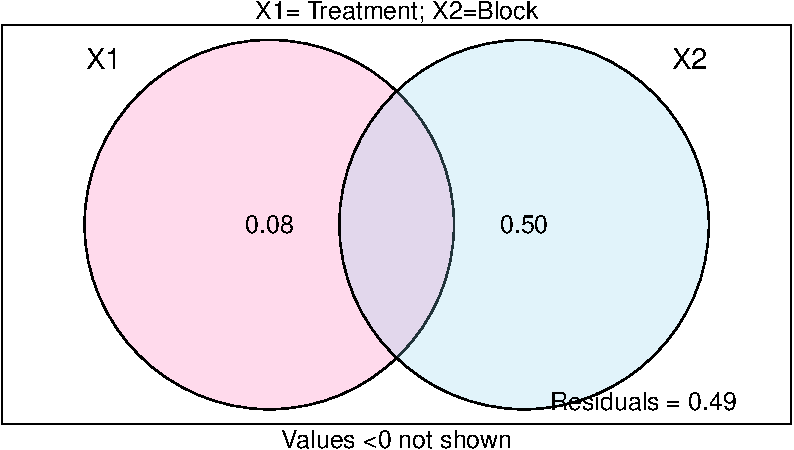
\includegraphics{log-project-aubrie-winnie_files/figure-latex/unnamed-chunk-4-2.pdf}

Composition dissimilarity * 2021 *

\begin{Shaded}
\begin{Highlighting}[]
\CommentTok{\# subset data where all t0 communities, insitu log and insitu open communities at t1 and t2 are included.}
\NormalTok{mat2 }\OtherTok{\textless{}{-}}\NormalTok{ mat[}\FunctionTok{which}\NormalTok{(mat}\SpecialCharTok{$}\NormalTok{time}\SpecialCharTok{==}\StringTok{"t1"} \SpecialCharTok{\&}\NormalTok{  mat}\SpecialCharTok{$}\NormalTok{treatment}\SpecialCharTok{==}\StringTok{"open"} \SpecialCharTok{|}\NormalTok{ mat}\SpecialCharTok{$}\NormalTok{time}\SpecialCharTok{==}\StringTok{"t1"} \SpecialCharTok{\&}\NormalTok{ mat}\SpecialCharTok{$}\NormalTok{treatment}\SpecialCharTok{==}\StringTok{"insitu\_log"}\NormalTok{),]}
\NormalTok{mat2}\SpecialCharTok{$}\NormalTok{grp}\OtherTok{\textless{}{-}}\FunctionTok{apply}\NormalTok{(mat2[}\FunctionTok{c}\NormalTok{(}\DecValTok{89}\NormalTok{,}\DecValTok{91}\NormalTok{)], }\DecValTok{1}\NormalTok{, paste, }\AttributeTok{collapse=}\StringTok{":"}\NormalTok{) }\CommentTok{\# block, init as grouping}
\CommentTok{\# names(mat2) \#check}

\CommentTok{\# another df where the grouping variables are time, block and initial state}
\CommentTok{\# each row is a transect in a certain year.}
\NormalTok{df}\OtherTok{\textless{}{-}}\NormalTok{mat2[,}\FunctionTok{c}\NormalTok{(}\DecValTok{1}\SpecialCharTok{:}\DecValTok{87}\NormalTok{, }\DecValTok{93}\NormalTok{)]}
\NormalTok{df2 }\OtherTok{=}\NormalTok{ df }\SpecialCharTok{\%\textgreater{}\%} \FunctionTok{mutate}\NormalTok{(}\FunctionTok{across}\NormalTok{(}\AttributeTok{.cols=}\DecValTok{1}\SpecialCharTok{:}\DecValTok{87}\NormalTok{,}\AttributeTok{.fns=}\NormalTok{as.numeric)) }\CommentTok{\# make everything numeric}
\FunctionTok{rownames}\NormalTok{(df2)}\OtherTok{\textless{}{-}}\ConstantTok{NULL} \CommentTok{\# remove rownames}

\DocumentationTok{\#\# new with group vars}
\NormalTok{nublock}\OtherTok{\textless{}{-}}\FunctionTok{separate}\NormalTok{(df2, }\DecValTok{88}\NormalTok{, }\FunctionTok{c}\NormalTok{(}\StringTok{"block"}\NormalTok{, }\StringTok{"init"}\NormalTok{), }\StringTok{":"}\NormalTok{) }\CommentTok{\# just looking at time, block \& initial treatment}

\CommentTok{\# want to sum across transects in same block X init treatment}
\NormalTok{nublock}\SpecialCharTok{$}\NormalTok{sumgrp}\OtherTok{\textless{}{-}}\FunctionTok{apply}\NormalTok{(mat2[}\FunctionTok{c}\NormalTok{(}\DecValTok{89}\NormalTok{, }\DecValTok{91}\NormalTok{)], }\DecValTok{1}\NormalTok{, paste, }\AttributeTok{collapse=}\StringTok{":"}\NormalTok{)}
\CommentTok{\# head(nublock)}

\CommentTok{\# sum observations across initial X  block (group variable)}
\CommentTok{\# this gives number of plants in each transect TYPE for each year in each block. should be 2 types X 3 years X 7 blocks rows }
\NormalTok{blocksum}\OtherTok{\textless{}{-}}\FunctionTok{rowsum}\NormalTok{(nublock[,}\FunctionTok{c}\NormalTok{(}\DecValTok{1}\SpecialCharTok{:}\DecValTok{87}\NormalTok{)], }\AttributeTok{group=}\NormalTok{nublock}\SpecialCharTok{$}\NormalTok{sumgrp)}
\NormalTok{blocksum}\SpecialCharTok{$}\NormalTok{grps}\OtherTok{\textless{}{-}}\FunctionTok{rownames}\NormalTok{(blocksum)}
\FunctionTok{rownames}\NormalTok{(blocksum)}\OtherTok{\textless{}{-}}\ConstantTok{NULL} \CommentTok{\# remove rownames}
\CommentTok{\# nrow(blocksum) \# it is 14 rows as expected }

\DocumentationTok{\#\#  expand again}
\NormalTok{blocksum}\OtherTok{\textless{}{-}}\FunctionTok{separate}\NormalTok{(blocksum, }\DecValTok{88}\NormalTok{, }\FunctionTok{c}\NormalTok{(}\StringTok{"block"}\NormalTok{, }\StringTok{"init"}\NormalTok{), }\StringTok{":"}\NormalTok{)}

\CommentTok{\# at the moment this includes where there were no plants ("x" column in matrix)}
\NormalTok{assemblies\_t1}\OtherTok{\textless{}{-}}\NormalTok{blocksum[,}\FunctionTok{c}\NormalTok{(}\DecValTok{1}\SpecialCharTok{:}\DecValTok{87}\NormalTok{)]}

\CommentTok{\# group {-} these are the treatment variables that need to be separately fed into the MDS analaysis from the community analysis.}
\NormalTok{group\_init}\OtherTok{\textless{}{-}}\NormalTok{blocksum}\SpecialCharTok{$}\NormalTok{init}
\NormalTok{group\_block}\OtherTok{\textless{}{-}}\NormalTok{blocksum}\SpecialCharTok{$}\NormalTok{block}

\CommentTok{\# MDS }
\NormalTok{ass.rel.t1}\OtherTok{\textless{}{-}}\FunctionTok{decostand}\NormalTok{(assemblies\_t1, }\AttributeTok{method=}\StringTok{\textquotesingle{}hel\textquotesingle{}}\NormalTok{) }\CommentTok{\#standardize assemblies }
\NormalTok{ass.rel.t1\_NMS }\OtherTok{\textless{}{-}} \FunctionTok{metaMDS}\NormalTok{(ass.rel.t1, }\AttributeTok{distance =} \StringTok{\textquotesingle{}bray\textquotesingle{}}\NormalTok{, }\AttributeTok{k =} \DecValTok{5}\NormalTok{) }\CommentTok{\# run MDS }
\end{Highlighting}
\end{Shaded}

\begin{verbatim}
## Run 0 stress 0.04139077 
## Run 1 stress 0.04155986 
## ... Procrustes: rmse 0.01108162  max resid 0.01865537 
## Run 2 stress 0.04139117 
## ... Procrustes: rmse 0.0003904674  max resid 0.0006394658 
## ... Similar to previous best
## Run 3 stress 0.04723361 
## Run 4 stress 0.04139094 
## ... Procrustes: rmse 0.0005041454  max resid 0.0008074514 
## ... Similar to previous best
## Run 5 stress 0.04139115 
## ... Procrustes: rmse 0.0004043461  max resid 0.000672686 
## ... Similar to previous best
## Run 6 stress 0.0413911 
## ... Procrustes: rmse 0.0006262601  max resid 0.0009962434 
## ... Similar to previous best
## Run 7 stress 0.04142321 
## ... Procrustes: rmse 0.003946757  max resid 0.006450584 
## ... Similar to previous best
## Run 8 stress 0.04139094 
## ... Procrustes: rmse 0.0002291748  max resid 0.0003509792 
## ... Similar to previous best
## Run 9 stress 0.04139106 
## ... Procrustes: rmse 0.0003431336  max resid 0.0005650645 
## ... Similar to previous best
## Run 10 stress 0.04139198 
## ... Procrustes: rmse 0.0007849452  max resid 0.001292057 
## ... Similar to previous best
## Run 11 stress 0.04139125 
## ... Procrustes: rmse 0.0004709341  max resid 0.0007752674 
## ... Similar to previous best
## Run 12 stress 0.0413909 
## ... Procrustes: rmse 0.0001931507  max resid 0.0003162998 
## ... Similar to previous best
## Run 13 stress 0.04143393 
## ... Procrustes: rmse 0.005523618  max resid 0.00902677 
## Run 14 stress 0.04139286 
## ... Procrustes: rmse 0.001110532  max resid 0.001824788 
## ... Similar to previous best
## Run 15 stress 0.04139107 
## ... Procrustes: rmse 0.0003521771  max resid 0.0005779692 
## ... Similar to previous best
## Run 16 stress 0.04139087 
## ... Procrustes: rmse 0.0003644169  max resid 0.0004738024 
## ... Similar to previous best
## Run 17 stress 0.04139107 
## ... Procrustes: rmse 0.0003481472  max resid 0.000574449 
## ... Similar to previous best
## Run 18 stress 0.0413912 
## ... Procrustes: rmse 0.0004310104  max resid 0.0007061979 
## ... Similar to previous best
## Run 19 stress 0.0413909 
## ... Procrustes: rmse 0.0004724183  max resid 0.0007578608 
## ... Similar to previous best
## Run 20 stress 0.04139106 
## ... Procrustes: rmse 0.0003257462  max resid 0.0005359794 
## ... Similar to previous best
## *** Best solution repeated 17 times
\end{verbatim}

\begin{Shaded}
\begin{Highlighting}[]
\CommentTok{\# stressplot(ass.rel.t1\_NMS) \# check fit}

\CommentTok{\# scores}
\NormalTok{mds\_scores\_t1}\OtherTok{\textless{}{-}}\FunctionTok{as.data.frame}\NormalTok{(vegan}\SpecialCharTok{::}\FunctionTok{scores}\NormalTok{(ass.rel.t1\_NMS)}\SpecialCharTok{$}\NormalTok{sites) }\CommentTok{\# extract scores}
\NormalTok{mds\_scores\_t1}\SpecialCharTok{$}\NormalTok{site}\OtherTok{\textless{}{-}}\FunctionTok{rownames}\NormalTok{(vegan}\SpecialCharTok{::}\FunctionTok{scores}\NormalTok{(ass.rel.t1\_NMS)}\SpecialCharTok{$}\NormalTok{sites) }\CommentTok{\# extract names }
\NormalTok{mds\_scores\_t1}\SpecialCharTok{$}\NormalTok{treatment}\OtherTok{\textless{}{-}}\NormalTok{group\_init }\CommentTok{\# grouping factor 1 }
\NormalTok{mds\_scores\_t1}\SpecialCharTok{$}\NormalTok{block}\OtherTok{\textless{}{-}}\NormalTok{group\_block }\CommentTok{\# grouping factor 2 }

\CommentTok{\# explaining factors}
\NormalTok{init}\OtherTok{\textless{}{-}}\FunctionTok{as.factor}\NormalTok{(group\_init) }\CommentTok{\# grouping factor 1{-} convert to factor}
\NormalTok{block}\OtherTok{\textless{}{-}}\FunctionTok{as.factor}\NormalTok{(group\_block) }\CommentTok{\# grouping factor 2{-} convert to factor}

\DocumentationTok{\#\#\#\# rda model analysis \& results \#\#\#\# }
\CommentTok{\# can look at significance of model where initial treatment and block explain variation in community}
\CommentTok{\# trt\_tot\_2\textless{}{-}rda(ass.rel.t1\textasciitilde{}init+block) \# run model using standardized data }
\CommentTok{\# summary(trt\_tot\_2)}
\CommentTok{\# anova.cca(trt\_tot\_2, step=1000, by="term") \#\# test for model significance}

\CommentTok{\# can model using varpart to look at contributions of initial treatment and block}
\NormalTok{var.mod2}\OtherTok{\textless{}{-}}\FunctionTok{varpart}\NormalTok{(ass.rel.t1, init, block) }\CommentTok{\# run model on standardized data}
\FunctionTok{plot}\NormalTok{(var.mod2, }\AttributeTok{bg=}\FunctionTok{c}\NormalTok{(}\StringTok{"hotpink"}\NormalTok{,}\StringTok{"skyblue"}\NormalTok{))}
\FunctionTok{mtext}\NormalTok{(}\StringTok{"X1= Treatment; X2=Block"}\NormalTok{, }\AttributeTok{side=}\DecValTok{3}\NormalTok{)}
\end{Highlighting}
\end{Shaded}

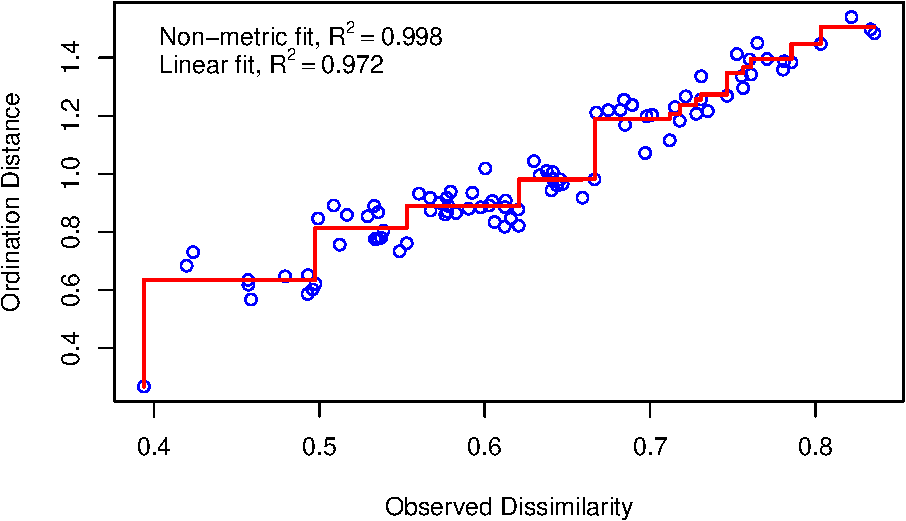
\includegraphics[width=30]{log-project-aubrie-winnie_files/figure-latex/unnamed-chunk-5-1}

\begin{Shaded}
\begin{Highlighting}[]
\DocumentationTok{\#\# can test for significance of contribution of the fraction of initial treatment}
\CommentTok{\# do this with partial redundancy analysis}
\NormalTok{trt\_Frac}\OtherTok{\textless{}{-}}\FunctionTok{rda}\NormalTok{(ass.rel.t1, init, block) }\CommentTok{\# partial rda model}
\FunctionTok{summary}\NormalTok{(trt\_Frac) }
\end{Highlighting}
\end{Shaded}

\begin{verbatim}
## 
## Call:
## rda(X = ass.rel.t1, Y = init, Z = block) 
## 
## Partitioning of variance:
##               Inertia Proportion
## Total         0.53262     1.0000
## Conditioned   0.28621     0.5373
## Constrained   0.06436     0.1208
## Unconstrained 0.18206     0.3418
## 
## Eigenvalues, and their contribution to the variance 
## after removing the contribution of conditiniong variables
## 
## Importance of components:
##                          RDA1     PC1     PC2     PC3     PC4     PC5     PC6
## Eigenvalue            0.06436 0.05497 0.03785 0.02947 0.02799 0.02046 0.01132
## Proportion Explained  0.26118 0.22307 0.15362 0.11959 0.11357 0.08304 0.04593
## Cumulative Proportion 0.26118 0.48425 0.63787 0.75745 0.87103 0.95407 1.00000
## 
## Accumulated constrained eigenvalues
## Importance of components:
##                          RDA1
## Eigenvalue            0.06436
## Proportion Explained  1.00000
## Cumulative Proportion 1.00000
## 
## Scaling 2 for species and site scores
## * Species are scaled proportional to eigenvalues
## * Sites are unscaled: weighted dispersion equal on all dimensions
## * General scaling constant of scores:  1.62215 
## 
## 
## Species scores
## 
##            RDA1        PC1        PC2        PC3        PC4        PC5
## acul   0.055571  3.637e-02  4.328e-02  1.783e-02  5.246e-03  5.454e-04
## aicu   0.000000  8.472e-17 -2.496e-17 -1.813e-17  2.580e-17 -2.616e-17
## arca   0.000000  9.597e-18  2.861e-18  1.596e-17 -2.682e-18 -9.970e-19
## ardy   0.042259  5.025e-02  5.860e-02  1.652e-02  4.875e-02  2.875e-02
## arsp   0.000000  1.984e-17  3.886e-17  5.839e-17 -3.819e-17  1.599e-17
## auel   0.000000  9.860e-19 -4.413e-18  8.306e-18 -3.824e-18 -6.153e-18
## bldr  -0.039796 -4.819e-03  3.972e-02 -4.794e-02 -2.337e-02  2.293e-02
## blrd   0.042899  4.726e-03  1.765e-02  2.217e-02 -5.565e-02 -2.605e-02
## brdi   0.000000 -1.170e-17 -1.637e-17 -2.608e-17 -3.440e-18 -2.426e-17
## brdr   0.000000 -2.443e-19  4.135e-18 -1.727e-18 -3.647e-18  3.050e-18
## brpe  -0.128276 -8.636e-02 -6.995e-02 -9.422e-02 -6.120e-02 -1.120e-02
## brru   0.000000 -1.871e-34  5.118e-33 -4.301e-33 -3.629e-33  2.180e-33
## buse   0.000000  5.868e-34 -1.605e-32  1.349e-32  1.138e-32 -6.838e-33
## caer   0.011258 -7.733e-02  7.189e-02  4.870e-03  3.834e-02 -9.362e-02
## cagr  -0.095632 -8.997e-02 -1.221e-02  1.902e-02 -2.621e-02 -1.103e-01
## cahi   0.000000  0.000e+00  0.000e+00  0.000e+00  0.000e+00  0.000e+00
## casp  -0.003109  1.770e-02 -2.479e-02 -2.422e-02  2.065e-02  6.085e-02
## cear   0.042899  2.468e-03 -6.751e-02  5.673e-02  4.787e-02 -2.876e-02
## chau   0.140877 -1.835e-01 -1.649e-02  1.254e-02  8.452e-02  1.746e-02
## chei   0.000000  0.000e+00  0.000e+00  0.000e+00  0.000e+00  0.000e+00
## chps   0.213452  9.333e-02  4.706e-02 -1.968e-02 -1.078e-01  1.722e-02
## crcl   0.000000  0.000e+00  0.000e+00  0.000e+00  0.000e+00  0.000e+00
## crco   0.138108  1.593e-01 -8.706e-02  4.536e-02 -1.939e-02  3.021e-02
## cusc   0.000000  0.000e+00  0.000e+00  0.000e+00  0.000e+00  0.000e+00
## cusp   0.023897  4.130e-03  2.468e-02  9.589e-02 -9.788e-02  9.619e-03
## dagl   0.000000  0.000e+00  0.000e+00  0.000e+00  0.000e+00  0.000e+00
## dosp   0.000000  0.000e+00  0.000e+00  0.000e+00  0.000e+00  0.000e+00
## ento   0.000000  0.000e+00  0.000e+00  0.000e+00  0.000e+00  0.000e+00
## erau   0.000000  0.000e+00  0.000e+00  0.000e+00  0.000e+00  0.000e+00
## ercy  -0.129183 -3.188e-02  1.257e-02  8.821e-02  5.864e-02  3.511e-02
## erra   0.021450 -2.405e-03 -1.984e-03  4.725e-03 -3.054e-02 -2.041e-02
## ersp   0.000000  0.000e+00  0.000e+00  0.000e+00  0.000e+00  0.000e+00
## gite  -0.059503  1.330e-01 -2.802e-02 -9.877e-04 -2.136e-02 -4.809e-02
## gnte   0.105088 -1.192e-01 -1.940e-02  3.043e-03  6.651e-02 -1.381e-03
## gobe   0.009616  2.117e-02  6.289e-02 -1.833e-01 -6.378e-02  4.242e-02
## gocy   0.000000  0.000e+00  0.000e+00  0.000e+00  0.000e+00  0.000e+00
## gono   0.000000  0.000e+00  0.000e+00  0.000e+00  0.000e+00  0.000e+00
## goro   0.087805  8.971e-02  6.801e-02 -8.319e-02  1.119e-01 -7.619e-02
## gosp   0.000000  0.000e+00  0.000e+00  0.000e+00  0.000e+00  0.000e+00
## haod  -0.032312 -2.971e-03 -4.026e-03  6.188e-02 -2.109e-02  4.142e-02
## hygl   0.215609  4.905e-02  1.609e-03  6.009e-02  1.333e-02  5.224e-02
## hypi  -0.035126 -4.177e-02 -4.871e-02 -1.374e-02 -4.052e-02 -2.390e-02
## hypo   0.000000  0.000e+00  0.000e+00  0.000e+00  0.000e+00  0.000e+00
## jubu   0.000000  0.000e+00  0.000e+00  0.000e+00  0.000e+00  0.000e+00
## laro  -0.062906 -4.731e-03  4.412e-02  2.142e-02 -5.523e-02  6.194e-02
## ledu   0.004284  1.424e-03  3.922e-03  3.485e-03 -5.014e-03 -1.127e-03
## lele   0.019834  1.824e-03  2.471e-03 -3.798e-02  1.295e-02 -2.543e-02
## loef   0.000000  0.000e+00  0.000e+00  0.000e+00  0.000e+00  0.000e+00
## misp  -0.077168 -1.527e-01  1.772e-02 -2.016e-02 -2.886e-02 -4.694e-02
## mite   0.000000  0.000e+00  0.000e+00  0.000e+00  0.000e+00  0.000e+00
## momo   0.000000  0.000e+00  0.000e+00  0.000e+00  0.000e+00  0.000e+00
## mopa   0.000000  0.000e+00  0.000e+00  0.000e+00  0.000e+00  0.000e+00
## niro  -0.036841 -1.225e-02 -3.373e-02 -2.997e-02  4.312e-02  9.689e-03
## omco   0.022017  1.488e-02 -2.711e-02 -1.869e-02 -1.512e-02  3.695e-02
## orsp   0.000000  0.000e+00  0.000e+00  0.000e+00  0.000e+00  0.000e+00
## pala   0.000000  0.000e+00  0.000e+00  0.000e+00  0.000e+00  0.000e+00
## peai   0.031786 -6.717e-02 -6.703e-02 -9.866e-02  1.006e-01  1.083e-01
## pedu   0.000000  0.000e+00  0.000e+00  0.000e+00  0.000e+00  0.000e+00
## phsu  -0.026050 -8.660e-03 -2.385e-02 -2.119e-02  3.049e-02  6.851e-03
## plde   0.000000  0.000e+00  0.000e+00  0.000e+00  0.000e+00  0.000e+00
## poar   0.006522 -1.086e-01  5.808e-02  2.807e-02  3.614e-02 -2.284e-02
## poca   0.000000  0.000e+00  0.000e+00  0.000e+00  0.000e+00  0.000e+00
## pocap  0.000000  0.000e+00  0.000e+00  0.000e+00  0.000e+00  0.000e+00
## poce   0.000000  0.000e+00  0.000e+00  0.000e+00  0.000e+00  0.000e+00
## pogn   0.000000  0.000e+00  0.000e+00  0.000e+00  0.000e+00  0.000e+00
## pole  -0.037141 -1.016e-01 -9.293e-02 -3.438e-02 -7.013e-02 -1.911e-02
## pomu   0.047780  9.595e-02  1.336e-01  5.875e-02  9.945e-02  8.749e-02
## pter   0.000000  0.000e+00  0.000e+00  0.000e+00  0.000e+00  0.000e+00
## ptga   0.126430 -1.396e-01  1.126e-03 -9.388e-03 -4.387e-02  5.596e-02
## ptob   0.000000  0.000e+00  0.000e+00  0.000e+00  0.000e+00  0.000e+00
## rhla   0.000000  0.000e+00  0.000e+00  0.000e+00  0.000e+00  0.000e+00
## rhpy  -0.080545 -6.671e-02 -9.829e-02  1.253e-01 -1.163e-01  2.039e-02
## rhsp   0.000000  0.000e+00  0.000e+00  0.000e+00  0.000e+00  0.000e+00
## ry     0.000000  0.000e+00  0.000e+00  0.000e+00  0.000e+00  0.000e+00
## scna   0.043870 -4.887e-02 -2.320e-02  2.874e-02  3.198e-02  3.740e-03
## sino   0.000000  0.000e+00  0.000e+00  0.000e+00  0.000e+00  0.000e+00
## sool  -0.032312 -2.971e-03 -4.026e-03  6.188e-02 -2.109e-02  4.142e-02
## stfi   0.000000  0.000e+00  0.000e+00  0.000e+00  0.000e+00  0.000e+00
## stpi   0.000000  0.000e+00  0.000e+00  0.000e+00  0.000e+00  0.000e+00
## thma   0.000000  0.000e+00  0.000e+00  0.000e+00  0.000e+00  0.000e+00
## trcy  -0.192212  8.297e-02 -2.570e-01 -7.513e-02  4.924e-02  3.987e-03
## tris   0.061108 -4.018e-02 -3.765e-02  9.554e-02  4.144e-02  1.226e-02
## tror  -0.092188 -2.616e-02  1.417e-01 -5.750e-02 -5.785e-02 -1.555e-02
## trpi  -0.084150  1.881e-01 -3.963e-02 -1.397e-03 -3.021e-02 -6.801e-02
## waac  -0.075766  3.898e-02 -3.149e-02  5.714e-02  8.339e-02 -1.179e-01
## wagr   0.056986  1.417e-02  3.648e-02 -7.759e-03 -3.054e-02 -3.520e-02
## x      0.022017  1.488e-02 -2.711e-02 -1.869e-02 -1.512e-02  3.695e-02
## 
## 
## Site scores (weighted sums of species scores)
## 
##          RDA1      PC1      PC2       PC3     PC4     PC5
## sit1  -0.3912 -0.29299  0.53388  0.367996  0.2978 -0.7276
## sit2   0.3912  0.29299 -0.53388 -0.367996 -0.2978  0.7276
## sit3  -0.4999  0.96887 -0.20417 -0.007197 -0.1556 -0.3504
## sit4   0.4999 -0.96887  0.20417  0.007197  0.1556  0.3504
## sit5  -0.5201 -0.14413 -0.39689 -0.352694  0.5075  0.1140
## sit6   0.5201  0.14413  0.39689  0.352694 -0.5075 -0.1140
## sit7  -0.2983  0.04860  0.04011 -0.095492  0.6173  0.4125
## sit8   0.2983 -0.04860 -0.04011  0.095492 -0.6173 -0.4125
## sit9  -0.6722 -0.51555 -0.60119 -0.169521 -0.5001 -0.2950
## sit10  0.6722  0.51555  0.60119  0.169521  0.5001  0.2950
## sit11 -0.3244 -0.03987 -0.05401  0.830224 -0.2830  0.5558
## sit12  0.3244  0.03987  0.05401 -0.830224  0.2830 -0.5558
## sit13 -0.3287 -0.02494  0.68227 -0.573317 -0.4838  0.2906
## sit14  0.3287  0.02494 -0.68227  0.573317  0.4838 -0.2906
## 
## 
## Site constraints (linear combinations of constraining variables)
## 
##          RDA1      PC1      PC2       PC3     PC4     PC5
## con1  -0.4335 -0.29299  0.53388  0.367996  0.2978 -0.7276
## con2   0.4335  0.29299 -0.53388 -0.367996 -0.2978  0.7276
## con3  -0.4335  0.96887 -0.20417 -0.007197 -0.1556 -0.3504
## con4   0.4335 -0.96887  0.20417  0.007197  0.1556  0.3504
## con5  -0.4335 -0.14413 -0.39689 -0.352694  0.5075  0.1140
## con6   0.4335  0.14413  0.39689  0.352694 -0.5075 -0.1140
## con7  -0.4335  0.04860  0.04011 -0.095492  0.6173  0.4125
## con8   0.4335 -0.04860 -0.04011  0.095492 -0.6173 -0.4125
## con9  -0.4335 -0.51555 -0.60119 -0.169521 -0.5001 -0.2950
## con10  0.4335  0.51555  0.60119  0.169521  0.5001  0.2950
## con11 -0.4335 -0.03987 -0.05401  0.830224 -0.2830  0.5558
## con12  0.4335  0.03987  0.05401 -0.830224  0.2830 -0.5558
## con13 -0.4335 -0.02494  0.68227 -0.573317 -0.4838  0.2906
## con14  0.4335  0.02494 -0.68227  0.573317  0.4838 -0.2906
## 
## 
## Biplot scores for constraining variables
## 
##       RDA1 PC1 PC2 PC3 PC4 PC5
## Yopen    1   0   0   0   0   0
\end{verbatim}

\begin{Shaded}
\begin{Highlighting}[]
\FunctionTok{RsquareAdj}\NormalTok{(trt\_Frac)}\SpecialCharTok{$}\NormalTok{adj.r.squared }\CommentTok{\#explanatory power}
\end{Highlighting}
\end{Shaded}

\begin{verbatim}
## [1] 0.1186067
\end{verbatim}

\begin{Shaded}
\begin{Highlighting}[]
\FunctionTok{anova.cca}\NormalTok{(trt\_Frac) }\DocumentationTok{\#\# this tells us if first condition, init, significantly contributes to overall variance explanation. }
\end{Highlighting}
\end{Shaded}

\begin{verbatim}
## Permutation test for rda under reduced model
## Permutation: free
## Number of permutations: 999
## 
## Model: rda(X = ass.rel.t1, Y = init, Z = block)
##          Df Variance     F Pr(>F)  
## Model     1 0.064359 2.121  0.043 *
## Residual  6 0.182059               
## ---
## Signif. codes:  0 '***' 0.001 '**' 0.01 '*' 0.05 '.' 0.1 ' ' 1
\end{verbatim}

\begin{Shaded}
\begin{Highlighting}[]
\DocumentationTok{\#\#\# extracting species scores and plotting }
\CommentTok{\# species scores}
\NormalTok{species.scores}\OtherTok{\textless{}{-}}\FunctionTok{as.data.frame}\NormalTok{(vegan}\SpecialCharTok{::}\FunctionTok{scores}\NormalTok{(ass.rel.t1\_NMS,}\StringTok{"species"}\NormalTok{)) }\DocumentationTok{\#\# some species don\textquotesingle{}t have scores}
\NormalTok{species.scores}\SpecialCharTok{$}\NormalTok{species}\OtherTok{\textless{}{-}}\FunctionTok{rownames}\NormalTok{(species.scores) }

\DocumentationTok{\#\#\# NMDS 1 and 2 }
\NormalTok{log}\OtherTok{\textless{}{-}}\NormalTok{mds\_scores\_t1[mds\_scores\_t1}\SpecialCharTok{$}\NormalTok{treatment }\SpecialCharTok{==} \StringTok{"log"}\NormalTok{, ][}\FunctionTok{chull}\NormalTok{(mds\_scores\_t1[mds\_scores\_t1}\SpecialCharTok{$}\NormalTok{treatment }\SpecialCharTok{==} 
                                                          \StringTok{"log"}\NormalTok{, }\FunctionTok{c}\NormalTok{(}\StringTok{"NMDS1"}\NormalTok{, }\StringTok{"NMDS2"}\NormalTok{)]), ]}

\NormalTok{open}\OtherTok{\textless{}{-}}\NormalTok{mds\_scores\_t1[mds\_scores\_t1}\SpecialCharTok{$}\NormalTok{treatment }\SpecialCharTok{==} \StringTok{"open"}\NormalTok{, ][}\FunctionTok{chull}\NormalTok{(mds\_scores\_t1[mds\_scores\_t1}\SpecialCharTok{$}\NormalTok{treatment }\SpecialCharTok{==} 
                                                               \StringTok{"open"}\NormalTok{, }\FunctionTok{c}\NormalTok{(}\StringTok{"NMDS1"}\NormalTok{, }\StringTok{"NMDS2"}\NormalTok{)]), ]}

\NormalTok{hulldat}\OtherTok{\textless{}{-}}\FunctionTok{rbind}\NormalTok{(log,open)}
 
\NormalTok{nmds.plot }\OtherTok{\textless{}{-}} \FunctionTok{ggplot}\NormalTok{()}\SpecialCharTok{+}
  \FunctionTok{theme\_bw}\NormalTok{()}\SpecialCharTok{+}
  \FunctionTok{theme}\NormalTok{(}\AttributeTok{panel.background =} \FunctionTok{element\_blank}\NormalTok{(),}
        \AttributeTok{panel.grid.major =} \FunctionTok{element\_blank}\NormalTok{(),  }\CommentTok{\#remove major{-}grid labels}
        \AttributeTok{panel.grid.minor =} \FunctionTok{element\_blank}\NormalTok{(),  }\CommentTok{\#remove minor{-}grid labels}
        \AttributeTok{plot.background =} \FunctionTok{element\_blank}\NormalTok{(), }
        \AttributeTok{axis.text =} \FunctionTok{element\_text}\NormalTok{(}\AttributeTok{size =} \DecValTok{15}\NormalTok{),}
        \AttributeTok{axis.title=}\FunctionTok{element\_text}\NormalTok{(}\AttributeTok{size=}\DecValTok{20}\NormalTok{),}
        \AttributeTok{legend.title=}\FunctionTok{element\_text}\NormalTok{(}\AttributeTok{size=}\DecValTok{20}\NormalTok{), }
        \AttributeTok{legend.text=}\FunctionTok{element\_text}\NormalTok{(}\AttributeTok{size=}\DecValTok{15}\NormalTok{))}\SpecialCharTok{+}
  \FunctionTok{geom\_text\_repel}\NormalTok{(}\AttributeTok{data=}\NormalTok{species.scores, }\FunctionTok{aes}\NormalTok{(NMDS1, NMDS2, }\AttributeTok{label=}\NormalTok{species), }\AttributeTok{alpha=}\FloatTok{0.9}\NormalTok{, }\AttributeTok{size=}\DecValTok{5}\NormalTok{, }\AttributeTok{col=}\StringTok{\textquotesingle{}darkgray\textquotesingle{}}\NormalTok{,}\AttributeTok{na.rm=}\ConstantTok{TRUE}\NormalTok{)}\SpecialCharTok{+}
  \FunctionTok{geom\_polygon}\NormalTok{(}\AttributeTok{data=}\NormalTok{hulldat, }\FunctionTok{aes}\NormalTok{(NMDS1, NMDS2, }\AttributeTok{fill=}\NormalTok{treatment, }\AttributeTok{group=}\NormalTok{treatment), }\AttributeTok{alpha=}\FloatTok{0.3}\NormalTok{)}\SpecialCharTok{+}\FunctionTok{scale\_fill\_manual}\NormalTok{(}\AttributeTok{values=}\FunctionTok{c}\NormalTok{(}\StringTok{"\#63A088"}\NormalTok{,}\StringTok{"\#56638A"}\NormalTok{), }\AttributeTok{name=}\StringTok{"Treatment"}\NormalTok{)}\SpecialCharTok{+}
  \FunctionTok{geom\_point}\NormalTok{(}\AttributeTok{data=}\NormalTok{mds\_scores\_t1, }\FunctionTok{aes}\NormalTok{(NMDS1, NMDS2, }\AttributeTok{shape=}\NormalTok{block, }\AttributeTok{col=}\NormalTok{treatment), }\AttributeTok{size=}\DecValTok{6}\NormalTok{)}\SpecialCharTok{+} \FunctionTok{scale\_shape\_manual}\NormalTok{(}\AttributeTok{values =} \FunctionTok{c}\NormalTok{(}\DecValTok{14}\NormalTok{,}\DecValTok{15}\NormalTok{,}\DecValTok{16}\NormalTok{,}\DecValTok{17}\NormalTok{,}\DecValTok{11}\NormalTok{,}\DecValTok{18}\NormalTok{,}\DecValTok{8}\NormalTok{), }\AttributeTok{name=}\StringTok{\textquotesingle{}Block\textquotesingle{}}\NormalTok{)}\SpecialCharTok{+}
  \FunctionTok{scale\_colour\_manual}\NormalTok{(}\AttributeTok{values=}\FunctionTok{c}\NormalTok{(}\StringTok{"\#63A088"}\NormalTok{,}\StringTok{"\#56638A"}\NormalTok{), }\AttributeTok{name=}\StringTok{"Treatment"}\NormalTok{) }\SpecialCharTok{+}
  \FunctionTok{labs}\NormalTok{(}\AttributeTok{title=}\FunctionTok{paste0}\NormalTok{(}\StringTok{"Stress: "}\NormalTok{, }\FunctionTok{round}\NormalTok{(ass.rel.t1\_NMS}\SpecialCharTok{$}\NormalTok{stress,}\DecValTok{3}\NormalTok{)))}

\FunctionTok{print}\NormalTok{(nmds.plot)}
\end{Highlighting}
\end{Shaded}

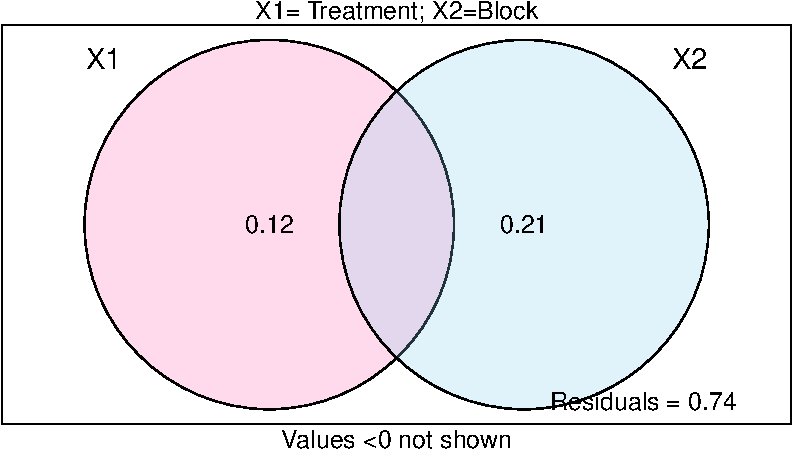
\includegraphics[width=30]{log-project-aubrie-winnie_files/figure-latex/unnamed-chunk-5-2}

\begin{Shaded}
\begin{Highlighting}[]
\CommentTok{\# All other NMDS pairs}
\NormalTok{treatments }\OtherTok{\textless{}{-}} \FunctionTok{unique}\NormalTok{(mds\_scores\_t1}\SpecialCharTok{$}\NormalTok{treatment)}
\NormalTok{plots }\OtherTok{\textless{}{-}} \FunctionTok{list}\NormalTok{()}
\NormalTok{num\_axes }\OtherTok{\textless{}{-}} \DecValTok{5}  

\ControlFlowTok{for}\NormalTok{ (i }\ControlFlowTok{in} \DecValTok{1}\SpecialCharTok{:}\NormalTok{num\_axes) \{}
  \ControlFlowTok{for}\NormalTok{ (j }\ControlFlowTok{in}\NormalTok{ (i}\SpecialCharTok{+}\DecValTok{1}\NormalTok{)}\SpecialCharTok{:}\NormalTok{num\_axes) \{  }
    \ControlFlowTok{if}\NormalTok{ (j }\SpecialCharTok{\textless{}=}\NormalTok{ num\_axes }\SpecialCharTok{\&\&}\NormalTok{ i }\SpecialCharTok{!=}\NormalTok{ j) \{  }
\NormalTok{      log }\OtherTok{\textless{}{-}}\NormalTok{ mds\_scores\_t1[mds\_scores\_t1}\SpecialCharTok{$}\NormalTok{treatment }\SpecialCharTok{==} \StringTok{"log"}\NormalTok{, ]}
\NormalTok{      open }\OtherTok{\textless{}{-}}\NormalTok{ mds\_scores\_t1[mds\_scores\_t1}\SpecialCharTok{$}\NormalTok{treatment }\SpecialCharTok{==} \StringTok{"open"}\NormalTok{, ]}
      
\NormalTok{      log\_hull }\OtherTok{\textless{}{-}}\NormalTok{ log[}\FunctionTok{chull}\NormalTok{(log[[}\FunctionTok{paste0}\NormalTok{(}\StringTok{"NMDS"}\NormalTok{, i)]], log[[}\FunctionTok{paste0}\NormalTok{(}\StringTok{"NMDS"}\NormalTok{, j)]]), ]}
\NormalTok{      open\_hull }\OtherTok{\textless{}{-}}\NormalTok{ open[}\FunctionTok{chull}\NormalTok{(open[[}\FunctionTok{paste0}\NormalTok{(}\StringTok{"NMDS"}\NormalTok{, i)]], open[[}\FunctionTok{paste0}\NormalTok{(}\StringTok{"NMDS"}\NormalTok{, j)]]), ]}
      
\NormalTok{      hulldat }\OtherTok{\textless{}{-}} \FunctionTok{rbind}\NormalTok{(log\_hull, open\_hull)}
      
\NormalTok{      plot\_name }\OtherTok{\textless{}{-}} \FunctionTok{paste0}\NormalTok{(i, }\StringTok{"+"}\NormalTok{, j)}
      
\NormalTok{      plots[[plot\_name]] }\OtherTok{\textless{}{-}} \FunctionTok{ggplot}\NormalTok{() }\SpecialCharTok{+}
        \FunctionTok{theme\_bw}\NormalTok{() }\SpecialCharTok{+}
        \FunctionTok{theme}\NormalTok{(}\AttributeTok{panel.background =} \FunctionTok{element\_blank}\NormalTok{(),}
              \AttributeTok{panel.grid.major =} \FunctionTok{element\_blank}\NormalTok{(),}
              \AttributeTok{panel.grid.minor =} \FunctionTok{element\_blank}\NormalTok{(),}
              \AttributeTok{plot.background =} \FunctionTok{element\_blank}\NormalTok{(),}
              \AttributeTok{axis.text =} \FunctionTok{element\_text}\NormalTok{(}\AttributeTok{size =} \DecValTok{15}\NormalTok{),}
              \AttributeTok{axis.title =} \FunctionTok{element\_text}\NormalTok{(}\AttributeTok{size =} \DecValTok{15}\NormalTok{),}
              \AttributeTok{legend.title =} \FunctionTok{element\_text}\NormalTok{(}\AttributeTok{size =} \DecValTok{15}\NormalTok{),}
              \AttributeTok{legend.text =} \FunctionTok{element\_text}\NormalTok{(}\AttributeTok{size =} \DecValTok{10}\NormalTok{)) }\SpecialCharTok{+}
        \FunctionTok{geom\_text\_repel}\NormalTok{(}\AttributeTok{data =}\NormalTok{ species.scores, }\FunctionTok{aes}\NormalTok{(}\AttributeTok{x =} \SpecialCharTok{!!}\FunctionTok{sym}\NormalTok{(}\FunctionTok{paste0}\NormalTok{(}\StringTok{"NMDS"}\NormalTok{, i)), }\AttributeTok{y =} \SpecialCharTok{!!}\FunctionTok{sym}\NormalTok{(}\FunctionTok{paste0}\NormalTok{(}\StringTok{"NMDS"}\NormalTok{, j)), }\AttributeTok{label =}\NormalTok{ species), }\AttributeTok{alpha =} \FloatTok{0.9}\NormalTok{, }\AttributeTok{size =} \DecValTok{3}\NormalTok{, }\AttributeTok{col =} \StringTok{\textquotesingle{}darkgray\textquotesingle{}}\NormalTok{, }\AttributeTok{na.rm =} \ConstantTok{TRUE}\NormalTok{) }\SpecialCharTok{+}
        \FunctionTok{geom\_polygon}\NormalTok{(}\AttributeTok{data =}\NormalTok{ hulldat, }\FunctionTok{aes}\NormalTok{(}\AttributeTok{x =} \SpecialCharTok{!!}\FunctionTok{sym}\NormalTok{(}\FunctionTok{paste0}\NormalTok{(}\StringTok{"NMDS"}\NormalTok{, i)), }\AttributeTok{y =} \SpecialCharTok{!!}\FunctionTok{sym}\NormalTok{(}\FunctionTok{paste0}\NormalTok{(}\StringTok{"NMDS"}\NormalTok{, j)), }\AttributeTok{fill =}\NormalTok{ treatment, }\AttributeTok{group =}\NormalTok{ treatment), }\AttributeTok{alpha =} \FloatTok{0.3}\NormalTok{) }\SpecialCharTok{+} \FunctionTok{scale\_fill\_manual}\NormalTok{(}\AttributeTok{values =} \FunctionTok{c}\NormalTok{(}\StringTok{"\#63A088"}\NormalTok{, }\StringTok{"\#56638A"}\NormalTok{), }\AttributeTok{name =} \StringTok{"Treatment"}\NormalTok{) }\SpecialCharTok{+}
        \FunctionTok{geom\_point}\NormalTok{(}\AttributeTok{data =}\NormalTok{ mds\_scores\_t1, }\FunctionTok{aes}\NormalTok{(}\AttributeTok{x =} \SpecialCharTok{!!}\FunctionTok{sym}\NormalTok{(}\FunctionTok{paste0}\NormalTok{(}\StringTok{"NMDS"}\NormalTok{, i)), }\AttributeTok{y =} \SpecialCharTok{!!}\FunctionTok{sym}\NormalTok{(}\FunctionTok{paste0}\NormalTok{(}\StringTok{"NMDS"}\NormalTok{, j)), }\AttributeTok{shape =}\NormalTok{ block, }\AttributeTok{col =}\NormalTok{ treatment), }\AttributeTok{size =} \DecValTok{6}\NormalTok{) }\SpecialCharTok{+} \FunctionTok{scale\_shape\_manual}\NormalTok{(}\AttributeTok{values =} \FunctionTok{c}\NormalTok{(}\DecValTok{14}\NormalTok{, }\DecValTok{15}\NormalTok{, }\DecValTok{16}\NormalTok{, }\DecValTok{17}\NormalTok{, }\DecValTok{11}\NormalTok{, }\DecValTok{18}\NormalTok{, }\DecValTok{8}\NormalTok{), }\AttributeTok{name =} \StringTok{\textquotesingle{}Block\textquotesingle{}}\NormalTok{) }\SpecialCharTok{+}
        \FunctionTok{scale\_colour\_manual}\NormalTok{(}\AttributeTok{values =} \FunctionTok{c}\NormalTok{(}\StringTok{"\#63A088"}\NormalTok{, }\StringTok{"\#56638A"}\NormalTok{), }\AttributeTok{name =} \StringTok{"Treatment"}\NormalTok{) }\SpecialCharTok{+}
        \FunctionTok{xlab}\NormalTok{(}\FunctionTok{paste0}\NormalTok{(}\StringTok{"NMDS"}\NormalTok{, i)) }\SpecialCharTok{+}
        \FunctionTok{ylab}\NormalTok{(}\FunctionTok{paste0}\NormalTok{(}\StringTok{"NMDS"}\NormalTok{, j))}
\NormalTok{    \}}
\NormalTok{  \}}
\NormalTok{\}}

\NormalTok{((plots}\SpecialCharTok{$}\StringTok{\textasciigrave{}}\AttributeTok{1+3}\StringTok{\textasciigrave{}} \SpecialCharTok{+}\NormalTok{ plots}\SpecialCharTok{$}\StringTok{\textasciigrave{}}\AttributeTok{1+4}\StringTok{\textasciigrave{}}\SpecialCharTok{+}\NormalTok{ plots}\SpecialCharTok{$}\StringTok{\textasciigrave{}}\AttributeTok{1+5}\StringTok{\textasciigrave{}}\NormalTok{)}\SpecialCharTok{/}\NormalTok{(plots}\SpecialCharTok{$}\StringTok{\textasciigrave{}}\AttributeTok{2+3}\StringTok{\textasciigrave{}} \SpecialCharTok{+}\NormalTok{ plots}\SpecialCharTok{$}\StringTok{\textasciigrave{}}\AttributeTok{2+4}\StringTok{\textasciigrave{}}\SpecialCharTok{+}\NormalTok{ plots}\SpecialCharTok{$}\StringTok{\textasciigrave{}}\AttributeTok{2+5}\StringTok{\textasciigrave{}}\NormalTok{)}\SpecialCharTok{/}\NormalTok{(plots}\SpecialCharTok{$}\StringTok{\textasciigrave{}}\AttributeTok{3+4}\StringTok{\textasciigrave{}} \SpecialCharTok{+}\NormalTok{ plots}\SpecialCharTok{$}\StringTok{\textasciigrave{}}\AttributeTok{3+5}\StringTok{\textasciigrave{}}\SpecialCharTok{+}\NormalTok{ plots}\SpecialCharTok{$}\StringTok{\textasciigrave{}}\AttributeTok{4+5}\StringTok{\textasciigrave{}}\NormalTok{)) }\SpecialCharTok{+} \FunctionTok{plot\_layout}\NormalTok{(}\AttributeTok{guides =}\StringTok{"collect"}\NormalTok{) }\SpecialCharTok{+} \FunctionTok{plot\_annotation}\NormalTok{(}\FunctionTok{paste0}\NormalTok{(}\StringTok{"Stress:"}\NormalTok{,}\FunctionTok{round}\NormalTok{(ass.rel.t1\_NMS}\SpecialCharTok{$}\NormalTok{stress,}\DecValTok{3}\NormalTok{), }\StringTok{" (k = 5)"}\NormalTok{))}
\end{Highlighting}
\end{Shaded}

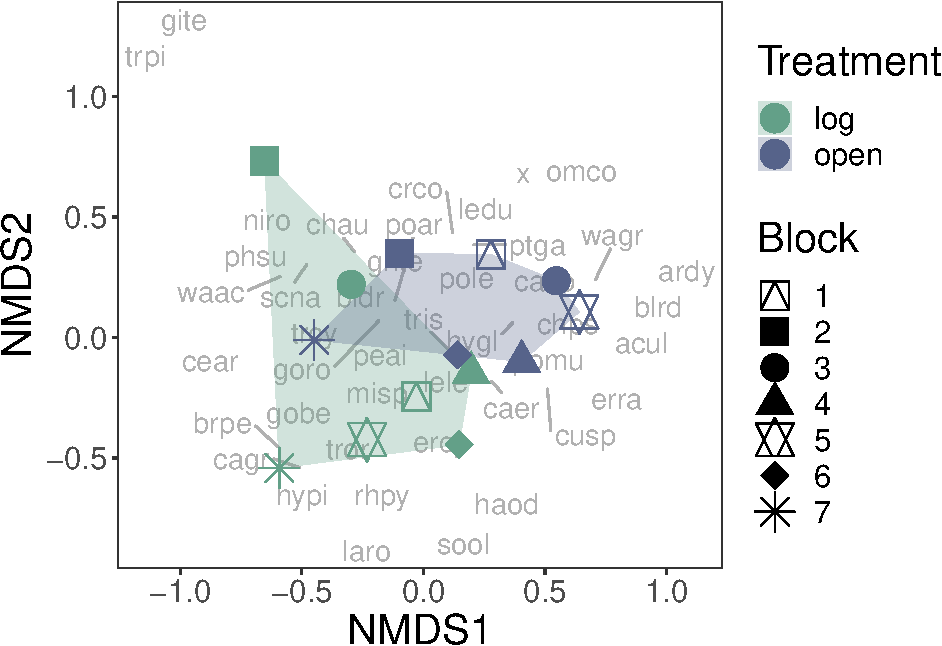
\includegraphics[width=100]{log-project-aubrie-winnie_files/figure-latex/unnamed-chunk-5-3}

Composition dissimilarity * 2022 *

\begin{Shaded}
\begin{Highlighting}[]
\CommentTok{\# subset data where all t0 communities, insitu log and insitu open communities at t1 and t2 are included.}
\NormalTok{mat2 }\OtherTok{\textless{}{-}}\NormalTok{ mat[}\FunctionTok{which}\NormalTok{(mat}\SpecialCharTok{$}\NormalTok{time}\SpecialCharTok{==}\StringTok{"t2"} \SpecialCharTok{\&}\NormalTok{  mat}\SpecialCharTok{$}\NormalTok{treatment}\SpecialCharTok{==}\StringTok{"open"} \SpecialCharTok{|}\NormalTok{ mat}\SpecialCharTok{$}\NormalTok{time}\SpecialCharTok{==}\StringTok{"t2"} \SpecialCharTok{\&}\NormalTok{ mat}\SpecialCharTok{$}\NormalTok{treatment}\SpecialCharTok{==}\StringTok{"insitu\_log"}\NormalTok{),]}
\NormalTok{mat2}\SpecialCharTok{$}\NormalTok{grp}\OtherTok{\textless{}{-}}\FunctionTok{apply}\NormalTok{(mat2[}\FunctionTok{c}\NormalTok{(}\DecValTok{89}\NormalTok{,}\DecValTok{91}\NormalTok{)], }\DecValTok{1}\NormalTok{, paste, }\AttributeTok{collapse=}\StringTok{":"}\NormalTok{) }\CommentTok{\# block, init as grouping}
\CommentTok{\# names(mat2) \#check}

\CommentTok{\# another df where the grouping variables are time, block and initial state}
\CommentTok{\# each row is a transect in a certain year.}
\NormalTok{df}\OtherTok{\textless{}{-}}\NormalTok{mat2[,}\FunctionTok{c}\NormalTok{(}\DecValTok{1}\SpecialCharTok{:}\DecValTok{87}\NormalTok{, }\DecValTok{93}\NormalTok{)]}
\NormalTok{df2 }\OtherTok{=}\NormalTok{ df }\SpecialCharTok{\%\textgreater{}\%} \FunctionTok{mutate}\NormalTok{(}\FunctionTok{across}\NormalTok{(}\AttributeTok{.cols=}\DecValTok{1}\SpecialCharTok{:}\DecValTok{87}\NormalTok{,}\AttributeTok{.fns=}\NormalTok{as.numeric)) }\CommentTok{\# make everything numeric}
\FunctionTok{rownames}\NormalTok{(df2)}\OtherTok{\textless{}{-}}\ConstantTok{NULL} \CommentTok{\# remove rownames}

\DocumentationTok{\#\# new with group vars}
\NormalTok{nublock}\OtherTok{\textless{}{-}}\FunctionTok{separate}\NormalTok{(df2, }\DecValTok{88}\NormalTok{, }\FunctionTok{c}\NormalTok{(}\StringTok{"block"}\NormalTok{, }\StringTok{"init"}\NormalTok{), }\StringTok{":"}\NormalTok{) }\CommentTok{\# just looking at time, block \& initial treatment}

\CommentTok{\# want to sum across transects in same block X init treatment}
\NormalTok{nublock}\SpecialCharTok{$}\NormalTok{sumgrp}\OtherTok{\textless{}{-}}\FunctionTok{apply}\NormalTok{(mat2[}\FunctionTok{c}\NormalTok{(}\DecValTok{89}\NormalTok{, }\DecValTok{91}\NormalTok{)], }\DecValTok{1}\NormalTok{, paste, }\AttributeTok{collapse=}\StringTok{":"}\NormalTok{)}
\CommentTok{\# head(nublock)}

\CommentTok{\# sum observations across initial X  block (group variable)}
\CommentTok{\# this gives number of plants in each transect TYPE for each year in each block. should be 2 types X 3 years X 7 blocks rows }
\NormalTok{blocksum}\OtherTok{\textless{}{-}}\FunctionTok{rowsum}\NormalTok{(nublock[,}\FunctionTok{c}\NormalTok{(}\DecValTok{1}\SpecialCharTok{:}\DecValTok{87}\NormalTok{)], }\AttributeTok{group=}\NormalTok{nublock}\SpecialCharTok{$}\NormalTok{sumgrp)}
\NormalTok{blocksum}\SpecialCharTok{$}\NormalTok{grps}\OtherTok{\textless{}{-}}\FunctionTok{rownames}\NormalTok{(blocksum)}
\FunctionTok{rownames}\NormalTok{(blocksum)}\OtherTok{\textless{}{-}}\ConstantTok{NULL} \CommentTok{\# remove rownames}
\CommentTok{\# nrow(blocksum) \# it is 14 rows as expected }

\DocumentationTok{\#\#  expand again}
\NormalTok{blocksum}\OtherTok{\textless{}{-}}\FunctionTok{separate}\NormalTok{(blocksum, }\DecValTok{88}\NormalTok{, }\FunctionTok{c}\NormalTok{(}\StringTok{"block"}\NormalTok{, }\StringTok{"init"}\NormalTok{), }\StringTok{":"}\NormalTok{)}

\CommentTok{\# at the moment this includes where there were no plants ("x" column in matrix)}
\NormalTok{assemblies\_t2}\OtherTok{\textless{}{-}}\NormalTok{blocksum[,}\FunctionTok{c}\NormalTok{(}\DecValTok{1}\SpecialCharTok{:}\DecValTok{87}\NormalTok{)]}

\CommentTok{\# group {-} these are the treatment variables that need to be separately fed into the MDS analaysis from the community analysis.}
\NormalTok{group\_init}\OtherTok{\textless{}{-}}\NormalTok{blocksum}\SpecialCharTok{$}\NormalTok{init}
\NormalTok{group\_block}\OtherTok{\textless{}{-}}\NormalTok{blocksum}\SpecialCharTok{$}\NormalTok{block}

\CommentTok{\# MDS }
\NormalTok{ass.rel.t2}\OtherTok{\textless{}{-}}\FunctionTok{decostand}\NormalTok{(assemblies\_t2, }\AttributeTok{method=}\StringTok{\textquotesingle{}hel\textquotesingle{}}\NormalTok{) }\CommentTok{\#standardize assemblies }
\NormalTok{ass.rel.t2\_NMS }\OtherTok{\textless{}{-}} \FunctionTok{metaMDS}\NormalTok{(ass.rel.t2, }\AttributeTok{distance =} \StringTok{\textquotesingle{}bray\textquotesingle{}}\NormalTok{, }\AttributeTok{k =} \DecValTok{4}\NormalTok{) }\CommentTok{\# run MDS }
\end{Highlighting}
\end{Shaded}

\begin{verbatim}
## Run 0 stress 0.03974779 
## Run 1 stress 0.0490994 
## Run 2 stress 0.03974766 
## ... New best solution
## ... Procrustes: rmse 0.0001127523  max resid 0.0002059325 
## ... Similar to previous best
## Run 3 stress 0.03974789 
## ... Procrustes: rmse 0.0001789641  max resid 0.0003241215 
## ... Similar to previous best
## Run 4 stress 0.0397477 
## ... Procrustes: rmse 4.148421e-05  max resid 7.558297e-05 
## ... Similar to previous best
## Run 5 stress 0.03974766 
## ... New best solution
## ... Procrustes: rmse 7.358159e-06  max resid 2.013283e-05 
## ... Similar to previous best
## Run 6 stress 0.03974772 
## ... Procrustes: rmse 5.424361e-05  max resid 9.884249e-05 
## ... Similar to previous best
## Run 7 stress 0.03974781 
## ... Procrustes: rmse 0.0005161603  max resid 0.0009514699 
## ... Similar to previous best
## Run 8 stress 0.03974769 
## ... Procrustes: rmse 0.0004145291  max resid 0.0007921542 
## ... Similar to previous best
## Run 9 stress 0.05604571 
## Run 10 stress 0.03974781 
## ... Procrustes: rmse 0.0005145371  max resid 0.0009527018 
## ... Similar to previous best
## Run 11 stress 0.050479 
## Run 12 stress 0.03974759 
## ... New best solution
## ... Procrustes: rmse 0.0001673963  max resid 0.0003044063 
## ... Similar to previous best
## Run 13 stress 0.03974783 
## ... Procrustes: rmse 0.0002982742  max resid 0.0005403872 
## ... Similar to previous best
## Run 14 stress 0.03974759 
## ... New best solution
## ... Procrustes: rmse 4.730376e-05  max resid 7.922382e-05 
## ... Similar to previous best
## Run 15 stress 0.03974779 
## ... Procrustes: rmse 0.0002307423  max resid 0.000420533 
## ... Similar to previous best
## Run 16 stress 0.03975381 
## ... Procrustes: rmse 0.001545361  max resid 0.003000333 
## ... Similar to previous best
## Run 17 stress 0.03974758 
## ... New best solution
## ... Procrustes: rmse 3.675266e-05  max resid 6.937286e-05 
## ... Similar to previous best
## Run 18 stress 0.03974777 
## ... Procrustes: rmse 0.0002537723  max resid 0.0004639752 
## ... Similar to previous best
## Run 19 stress 0.03974769 
## ... Procrustes: rmse 0.0001664545  max resid 0.0003082117 
## ... Similar to previous best
## Run 20 stress 0.03974763 
## ... Procrustes: rmse 0.0001891951  max resid 0.0003687155 
## ... Similar to previous best
## *** Best solution repeated 4 times
\end{verbatim}

\begin{Shaded}
\begin{Highlighting}[]
\CommentTok{\# stressplot(ass.rel.t2\_NMS) \# check fit}

\CommentTok{\# scores}
\NormalTok{mds\_scores\_t2}\OtherTok{\textless{}{-}}\FunctionTok{as.data.frame}\NormalTok{(vegan}\SpecialCharTok{::}\FunctionTok{scores}\NormalTok{(ass.rel.t2\_NMS)}\SpecialCharTok{$}\NormalTok{sites) }\CommentTok{\# extract scores}
\NormalTok{mds\_scores\_t2}\SpecialCharTok{$}\NormalTok{site}\OtherTok{\textless{}{-}}\FunctionTok{rownames}\NormalTok{(vegan}\SpecialCharTok{::}\FunctionTok{scores}\NormalTok{(ass.rel.t2\_NMS)}\SpecialCharTok{$}\NormalTok{sites) }\CommentTok{\# extract names }
\NormalTok{mds\_scores\_t2}\SpecialCharTok{$}\NormalTok{treatment}\OtherTok{\textless{}{-}}\NormalTok{group\_init }\CommentTok{\# grouping factor 1 }
\NormalTok{mds\_scores\_t2}\SpecialCharTok{$}\NormalTok{block}\OtherTok{\textless{}{-}}\NormalTok{group\_block }\CommentTok{\# grouping factor 2 }

\CommentTok{\# explaining factors}
\NormalTok{init}\OtherTok{\textless{}{-}}\FunctionTok{as.factor}\NormalTok{(group\_init) }\CommentTok{\# grouping factor 1{-} convert to factor}
\NormalTok{block}\OtherTok{\textless{}{-}}\FunctionTok{as.factor}\NormalTok{(group\_block) }\CommentTok{\# grouping factor 2{-} convert to factor}

\DocumentationTok{\#\#\#\# rda model analysis \& results \#\#\#\# }
\CommentTok{\# can look at significance of model where initial treatment and block explain variation in community}
\NormalTok{trt\_tot\_2}\OtherTok{\textless{}{-}}\FunctionTok{rda}\NormalTok{(ass.rel.t2}\SpecialCharTok{\textasciitilde{}}\NormalTok{init}\SpecialCharTok{+}\NormalTok{block) }\CommentTok{\# run model using standardized data }
\FunctionTok{summary}\NormalTok{(trt\_tot\_2)}
\end{Highlighting}
\end{Shaded}

\begin{verbatim}
## 
## Call:
## rda(formula = ass.rel.t2 ~ init + block) 
## 
## Partitioning of variance:
##               Inertia Proportion
## Total          0.5340     1.0000
## Constrained    0.3581     0.6705
## Unconstrained  0.1759     0.3295
## 
## Eigenvalues, and their contribution to the variance 
## 
## Importance of components:
##                         RDA1    RDA2    RDA3    RDA4    RDA5    RDA6    RDA7
## Eigenvalue            0.1078 0.07881 0.05379 0.04086 0.03384 0.02612 0.01683
## Proportion Explained  0.2019 0.14758 0.10073 0.07651 0.06338 0.04891 0.03151
## Cumulative Proportion 0.2019 0.34951 0.45024 0.52675 0.59013 0.63904 0.67055
##                          PC1     PC2     PC3     PC4     PC5     PC6
## Eigenvalue            0.0547 0.03572 0.03141 0.02309 0.01636 0.01464
## Proportion Explained  0.1024 0.06689 0.05882 0.04325 0.03064 0.02742
## Cumulative Proportion 0.7730 0.83988 0.89870 0.94194 0.97258 1.00000
## 
## Accumulated constrained eigenvalues
## Importance of components:
##                         RDA1    RDA2    RDA3    RDA4    RDA5    RDA6    RDA7
## Eigenvalue            0.1078 0.07881 0.05379 0.04086 0.03384 0.02612 0.01683
## Proportion Explained  0.3011 0.22009 0.15022 0.11410 0.09452 0.07293 0.04699
## Cumulative Proportion 0.3011 0.52124 0.67146 0.78556 0.88007 0.95301 1.00000
## 
## Scaling 2 for species and site scores
## * Species are scaled proportional to eigenvalues
## * Sites are unscaled: weighted dispersion equal on all dimensions
## * General scaling constant of scores:  1.623197 
## 
## 
## Species scores
## 
##             RDA1       RDA2       RDA3       RDA4       RDA5       RDA6
## acul   9.052e-02 -6.166e-02 -2.465e-02  1.043e-01  1.350e-01  9.105e-02
## aicu   4.768e-17  4.052e-17 -9.248e-17 -1.056e-17 -1.453e-17 -3.522e-18
## arca  -5.475e-17 -2.441e-18 -4.889e-17  1.376e-17 -1.781e-17  5.141e-17
## ardy  -4.584e-02 -4.434e-02 -1.111e-02  1.969e-02 -2.105e-02 -1.788e-02
## arsp  -1.390e-17  6.109e-19 -1.670e-17  5.467e-17  3.549e-17  3.880e-17
## auel  -1.762e-17  3.587e-17  1.566e-17 -1.261e-17 -4.081e-17 -4.764e-17
## bldr   1.039e-01  4.551e-02 -1.034e-02  5.410e-02  3.353e-02 -5.643e-02
## blrd   1.876e-17 -2.147e-17  1.438e-18  1.943e-17  2.607e-17  1.106e-17
## brdi   1.852e-02  3.590e-02  8.983e-03  2.044e-02  1.514e-03 -4.940e-02
## brdr   6.717e-18 -2.173e-18  1.097e-18  1.249e-18  4.221e-18 -1.502e-17
## brpe   1.354e-17  2.728e-17  4.933e-18  1.483e-17  1.682e-19 -3.402e-17
## brru  -7.711e-33  1.305e-32  2.283e-33  3.454e-33 -6.606e-33  1.260e-32
## buse   2.953e-33 -1.069e-32  2.015e-33 -2.537e-33  5.339e-33 -8.503e-33
## caer   1.272e-01 -6.922e-02  1.166e-01  7.445e-02  2.762e-02  4.229e-03
## cagr   0.000e+00  0.000e+00  0.000e+00  0.000e+00  0.000e+00  0.000e+00
## cahi   2.197e-02 -8.344e-02  7.037e-02  5.156e-02 -1.853e-02 -2.675e-02
## casp   0.000e+00  0.000e+00  0.000e+00  0.000e+00  0.000e+00  0.000e+00
## cear   0.000e+00  0.000e+00  0.000e+00  0.000e+00  0.000e+00  0.000e+00
## chau   0.000e+00  0.000e+00  0.000e+00  0.000e+00  0.000e+00  0.000e+00
## chei  -6.027e-02  4.108e-02 -1.022e-01  5.789e-02 -9.473e-02  3.468e-02
## chps   1.422e-01  5.056e-02 -9.443e-02 -2.245e-02  2.895e-02 -2.191e-02
## crcl   7.114e-02 -4.012e-02  4.716e-02 -3.862e-02 -7.741e-02  8.715e-03
## crco   9.734e-02 -6.815e-02 -1.138e-01  5.228e-02  9.551e-02 -5.560e-03
## cusc   9.947e-02 -4.263e-02  1.155e-01 -3.845e-02 -1.031e-01 -3.646e-02
## cusp   0.000e+00  0.000e+00  0.000e+00  0.000e+00  0.000e+00  0.000e+00
## dagl   0.000e+00  0.000e+00  0.000e+00  0.000e+00  0.000e+00  0.000e+00
## dosp  -1.315e-01 -1.124e-01 -1.082e-01  5.196e-02 -4.110e-02 -7.973e-02
## ento   0.000e+00  0.000e+00  0.000e+00  0.000e+00  0.000e+00  0.000e+00
## erau   3.620e-02 -3.512e-02  4.765e-02 -2.634e-02 -4.680e-02  5.787e-03
## ercy   4.416e-02 -5.421e-03 -7.098e-02 -1.592e-01  9.063e-02  1.565e-02
## erra   2.116e-02  3.187e-02 -5.398e-02 -1.259e-02  2.466e-02 -1.379e-02
## ersp   0.000e+00  0.000e+00  0.000e+00  0.000e+00  0.000e+00  0.000e+00
## gite  -2.639e-02 -2.973e-02 -6.122e-02  2.699e-02 -3.764e-02 -2.222e-02
## gnte   0.000e+00  0.000e+00  0.000e+00  0.000e+00  0.000e+00  0.000e+00
## gobe  -1.559e-01  1.913e-01  1.457e-01 -2.624e-03 -2.945e-02  7.403e-02
## gocy   0.000e+00  0.000e+00  0.000e+00  0.000e+00  0.000e+00  0.000e+00
## gono   0.000e+00  0.000e+00  0.000e+00  0.000e+00  0.000e+00  0.000e+00
## goro  -8.288e-03  1.152e-01 -1.390e-01  5.549e-02 -1.156e-01  3.310e-02
## gosp   0.000e+00  0.000e+00  0.000e+00  0.000e+00  0.000e+00  0.000e+00
## haod  -9.922e-04  1.618e-01 -1.355e-02 -1.014e-02  4.472e-02 -7.729e-02
## hygl   6.118e-02  9.387e-02  4.443e-02 -1.767e-02 -1.196e-02 -1.030e-01
## hypi   0.000e+00  0.000e+00  0.000e+00  0.000e+00  0.000e+00  0.000e+00
## hypo  -1.494e-01 -1.129e-01  6.094e-02 -1.241e-01 -4.803e-02  2.488e-02
## jubu   0.000e+00  0.000e+00  0.000e+00  0.000e+00  0.000e+00  0.000e+00
## laro  -5.349e-02 -2.490e-02  4.872e-02  4.252e-02 -7.231e-03 -7.957e-02
## ledu   0.000e+00  0.000e+00  0.000e+00  0.000e+00  0.000e+00  0.000e+00
## lele   0.000e+00  0.000e+00  0.000e+00  0.000e+00  0.000e+00  0.000e+00
## loef  -2.155e-02 -2.427e-02 -4.998e-02  2.204e-02 -3.073e-02 -1.814e-02
## misp   0.000e+00  0.000e+00  0.000e+00  0.000e+00  0.000e+00  0.000e+00
## mite  -1.261e-01  1.544e-01  1.114e-01 -9.659e-03  1.890e-01  3.377e-02
## momo   0.000e+00  0.000e+00  0.000e+00  0.000e+00  0.000e+00  0.000e+00
## mopa   0.000e+00  0.000e+00  0.000e+00  0.000e+00  0.000e+00  0.000e+00
## niro   0.000e+00  0.000e+00  0.000e+00  0.000e+00  0.000e+00  0.000e+00
## omco   0.000e+00  0.000e+00  0.000e+00  0.000e+00  0.000e+00  0.000e+00
## orsp  -5.409e-03  1.374e-02  4.231e-02  1.614e-02  9.775e-03 -4.362e-02
## pala   0.000e+00  0.000e+00  0.000e+00  0.000e+00  0.000e+00  0.000e+00
## peai  -1.076e-01  3.483e-01 -1.470e-01 -5.028e-02 -1.466e-02 -3.413e-02
## pedu   0.000e+00  0.000e+00  0.000e+00  0.000e+00  0.000e+00  0.000e+00
## phsu   0.000e+00  0.000e+00  0.000e+00  0.000e+00  0.000e+00  0.000e+00
## plde   0.000e+00  0.000e+00  0.000e+00  0.000e+00  0.000e+00  0.000e+00
## poar   0.000e+00  0.000e+00  0.000e+00  0.000e+00  0.000e+00  0.000e+00
## poca  -7.330e-02  1.228e-02 -1.627e-02 -1.762e-01  1.119e-01 -9.665e-02
## pocap -9.137e-02  1.421e-02 -2.497e-02  4.681e-02 -6.872e-02  3.860e-02
## poce  -5.409e-03  1.374e-02  4.231e-02  1.614e-02  9.775e-03 -4.362e-02
## pogn   0.000e+00  0.000e+00  0.000e+00  0.000e+00  0.000e+00  0.000e+00
## pole   5.618e-02 -1.627e-01 -9.388e-02 -1.303e-01  5.130e-02  8.606e-03
## pomu   4.919e-01  5.095e-02  2.181e-03 -4.628e-02 -5.128e-02 -4.981e-02
## pter   8.015e-02  4.723e-02 -2.287e-02 -4.203e-03 -2.753e-02 -5.322e-02
## ptga   1.310e-02  2.539e-02  6.352e-03  1.445e-02  1.071e-03 -3.493e-02
## ptob   0.000e+00  0.000e+00  0.000e+00  0.000e+00  0.000e+00  0.000e+00
## rhla   2.267e-02 -6.908e-02  4.303e-02  6.541e-02  8.281e-02  6.017e-02
## rhpy   1.001e-03  5.611e-02  1.010e-01  5.055e-02  2.293e-02 -1.325e-01
## rhsp  -2.148e-01 -1.818e-01 -9.260e-02 -9.215e-02 -2.889e-02 -6.196e-02
## ry     0.000e+00  0.000e+00  0.000e+00  0.000e+00  0.000e+00  0.000e+00
## scna   0.000e+00  0.000e+00  0.000e+00  0.000e+00  0.000e+00  0.000e+00
## sino   3.620e-02 -3.512e-02  4.765e-02 -2.634e-02 -4.680e-02  5.787e-03
## sool   0.000e+00  0.000e+00  0.000e+00  0.000e+00  0.000e+00  0.000e+00
## stfi  -5.409e-03  1.374e-02  4.231e-02  1.614e-02  9.775e-03 -4.362e-02
## stpi   0.000e+00  0.000e+00  0.000e+00  0.000e+00  0.000e+00  0.000e+00
## thma   0.000e+00  0.000e+00  0.000e+00  0.000e+00  0.000e+00  0.000e+00
## trcy  -1.561e-01 -1.095e-01  2.729e-02  1.591e-01  4.816e-02 -1.420e-01
## tris   4.228e-02 -1.673e-02 -2.024e-02  4.110e-02  3.757e-02  3.527e-02
## tror  -5.230e-02  8.443e-02  1.375e-01  8.368e-03 -4.656e-02  3.086e-02
## trpi   0.000e+00  0.000e+00  0.000e+00  0.000e+00  0.000e+00  0.000e+00
## waac  -1.822e-02 -3.727e-02  1.688e-01 -1.391e-01 -3.077e-02 -1.163e-02
## wagr   0.000e+00  0.000e+00  0.000e+00  0.000e+00  0.000e+00  0.000e+00
## x      0.000e+00  0.000e+00  0.000e+00  0.000e+00  0.000e+00  0.000e+00
## 
## 
## Site scores (weighted sums of species scores)
## 
##            RDA1     RDA2    RDA3     RDA4     RDA5     RDA6
## row1  -0.529954 -0.50054  0.2468 -1.10353  0.14120  0.29241
## row2   0.027932  0.29494 -0.3213 -0.55623  0.49222 -0.18686
## row3  -0.526506 -0.90064 -0.2668  0.49320 -0.41943 -0.57329
## row4  -0.521497 -0.16611 -0.6799  0.15480 -0.38435  0.01384
## row5   0.523959 -0.45922  0.7665 -0.33398 -1.07139  0.06484
## row6   0.751980 -0.09337 -0.1892 -0.28283 -0.23276  0.07611
## row7  -0.131864  0.32707 -0.1624 -0.14669  0.60202 -0.12836
## row8   0.300694  0.18578 -0.6404 -0.21465  0.18647 -0.22795
## row9  -0.083385 -0.56645  0.3037  0.69285  1.18053  0.55202
## row10  0.816213 -0.18975 -0.2365  0.35601 -0.04331  0.37932
## row11  0.004328  0.36280  0.7414  0.20897  0.15651 -0.81764
## row12  0.187756  0.43299  0.1371  0.38949  0.03776 -0.70925
## row13 -0.590590  0.63290  0.4722  0.06967 -0.07356  0.61728
## row14 -0.229066  0.63960 -0.1712  0.27293 -0.57192  0.64753
## 
## 
## Site constraints (linear combinations of constraining variables)
## 
##           RDA1     RDA2     RDA3    RDA4     RDA5     RDA6
## row1  -0.44158 -0.26053  0.26294 -0.8470  0.39041  0.05381
## row2  -0.06044  0.05493 -0.33743 -0.8128  0.24301  0.05174
## row3  -0.71457 -0.69110 -0.17315  0.3069 -0.32819 -0.27869
## row4  -0.33343 -0.37564 -0.77353  0.3411 -0.47559 -0.28076
## row5   0.44740 -0.43402  0.58885 -0.3255 -0.57837  0.07151
## row6   0.82854 -0.11857 -0.01153 -0.2913 -0.72577  0.06944
## row7  -0.10616  0.09870 -0.10123 -0.1977  0.46794 -0.17712
## row8   0.27499  0.41415 -0.70160 -0.1636  0.32055 -0.17919
## row9   0.17584 -0.53583  0.33379  0.5074  0.64231  0.46671
## row10  0.55699 -0.22037 -0.26659  0.5415  0.49491  0.46464
## row11 -0.09453  0.24017  0.73940  0.2822  0.17083 -0.76241
## row12  0.28661  0.55562  0.13902  0.3163  0.02343 -0.76448
## row13 -0.60040  0.47852  0.45072  0.1542 -0.24904  0.63344
## row14 -0.21925  0.79398 -0.14966  0.1884 -0.39644  0.63137
## 
## 
## Biplot scores for constraining variables
## 
##              RDA1    RDA2     RDA3     RDA4     RDA5      RDA6
## initopen  0.43929  0.3636 -0.69197  0.03936 -0.16988 -0.002386
## block2   -0.49312 -0.5019 -0.44544  0.30490 -0.37820 -0.263238
## block3    0.60037 -0.2600  0.27165 -0.29023 -0.61364  0.066324
## block4    0.07944  0.2413 -0.37775 -0.17002  0.37101 -0.167656
## block5    0.34482 -0.3558  0.03162  0.49352  0.53510  0.438225
## block6    0.09038  0.3744  0.41332  0.28159  0.09141 -0.718450
## block7   -0.38567  0.5987  0.14166  0.16120 -0.30372  0.595132
## 
## 
## Centroids for factor constraints
## 
##              RDA1    RDA2     RDA3     RDA4     RDA5      RDA6
## initlog  -0.19057 -0.1577  0.30019 -0.01707  0.07370  0.001035
## initopen  0.19057  0.1577 -0.30019  0.01707 -0.07370 -0.001035
## block1   -0.25101 -0.1028 -0.03724 -0.82988  0.31671  0.052774
## block2   -0.52400 -0.5334 -0.47334  0.32400 -0.40189 -0.279725
## block3    0.63797 -0.2763  0.28866 -0.30841 -0.65207  0.070478
## block4    0.08441  0.2564 -0.40141 -0.18067  0.39425 -0.178156
## block5    0.36641 -0.3781  0.03360  0.52443  0.56861  0.465671
## block6    0.09604  0.3979  0.43921  0.29923  0.09713 -0.763447
## block7   -0.40983  0.6363  0.15053  0.17130 -0.32274  0.632406
\end{verbatim}

\begin{Shaded}
\begin{Highlighting}[]
\FunctionTok{anova.cca}\NormalTok{(trt\_tot\_2, }\AttributeTok{step=}\DecValTok{1000}\NormalTok{, }\AttributeTok{by=}\StringTok{"term"}\NormalTok{) }\DocumentationTok{\#\# test for model significance}
\end{Highlighting}
\end{Shaded}

\begin{verbatim}
## Permutation test for rda under reduced model
## Terms added sequentially (first to last)
## Permutation: free
## Number of permutations: 999
## 
## Model: rda(formula = ass.rel.t2 ~ init + block)
##          Df Variance      F Pr(>F)   
## init      1  0.06081 2.0739  0.011 * 
## block     6  0.29726 1.6897  0.004 **
## Residual  6  0.17593                 
## ---
## Signif. codes:  0 '***' 0.001 '**' 0.01 '*' 0.05 '.' 0.1 ' ' 1
\end{verbatim}

\begin{Shaded}
\begin{Highlighting}[]
\CommentTok{\# can model using varpart to look at contributions of initial treatment and block}
\NormalTok{var.mod2}\OtherTok{\textless{}{-}}\FunctionTok{varpart}\NormalTok{(ass.rel.t2, init, block) }\CommentTok{\# run model on standardized data}
\FunctionTok{plot}\NormalTok{(var.mod2, }\AttributeTok{bg=}\FunctionTok{c}\NormalTok{(}\StringTok{"hotpink"}\NormalTok{,}\StringTok{"skyblue"}\NormalTok{))}
\FunctionTok{mtext}\NormalTok{(}\StringTok{"X1= Treatment; X2=Block"}\NormalTok{, }\AttributeTok{side=}\DecValTok{3}\NormalTok{)}
\end{Highlighting}
\end{Shaded}

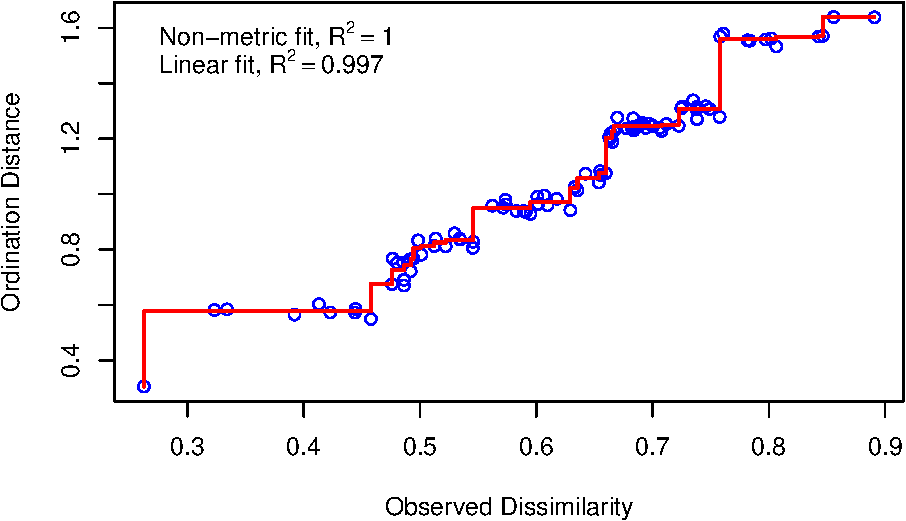
\includegraphics{log-project-aubrie-winnie_files/figure-latex/unnamed-chunk-6-1.pdf}

\begin{Shaded}
\begin{Highlighting}[]
\DocumentationTok{\#\# can test for significance of contribution of the fraction of initial treatment}
\CommentTok{\# do this with partial redundancy analysis}
\NormalTok{trt\_Frac}\OtherTok{\textless{}{-}}\FunctionTok{rda}\NormalTok{(ass.rel.t2, init, block) }\CommentTok{\# partial rda model}
\FunctionTok{summary}\NormalTok{(trt\_Frac) }
\end{Highlighting}
\end{Shaded}

\begin{verbatim}
## 
## Call:
## rda(X = ass.rel.t2, Y = init, Z = block) 
## 
## Partitioning of variance:
##               Inertia Proportion
## Total         0.53400     1.0000
## Conditioned   0.29726     0.5567
## Constrained   0.06081     0.1139
## Unconstrained 0.17593     0.3295
## 
## Eigenvalues, and their contribution to the variance 
## after removing the contribution of conditiniong variables
## 
## Importance of components:
##                          RDA1    PC1     PC2     PC3     PC4     PC5     PC6
## Eigenvalue            0.06081 0.0547 0.03572 0.03141 0.02309 0.01636 0.01464
## Proportion Explained  0.25687 0.2311 0.15089 0.13267 0.09755 0.06910 0.06185
## Cumulative Proportion 0.25687 0.4879 0.63882 0.77149 0.86905 0.93815 1.00000
## 
## Accumulated constrained eigenvalues
## Importance of components:
##                          RDA1
## Eigenvalue            0.06081
## Proportion Explained  1.00000
## Cumulative Proportion 1.00000
## 
## Scaling 2 for species and site scores
## * Species are scaled proportional to eigenvalues
## * Sites are unscaled: weighted dispersion equal on all dimensions
## * General scaling constant of scores:  1.623197 
## 
## 
## Species scores
## 
##            RDA1        PC1        PC2        PC3        PC4        PC5
## acul   0.020175 -2.142e-02 -8.157e-03 -2.565e-02 -6.560e-03 -2.267e-02
## aicu   0.000000 -4.876e-17 -4.519e-17 -3.653e-17  6.908e-18 -1.928e-17
## arca   0.000000 -8.942e-18  4.164e-17  3.659e-17  9.181e-18 -7.967e-18
## ardy  -0.027831 -4.756e-02 -3.944e-02  8.675e-03 -1.186e-02  5.108e-03
## arsp   0.000000 -2.014e-17 -2.380e-19 -1.365e-17  1.358e-17  1.535e-17
## auel   0.000000 -4.771e-18 -4.237e-19 -5.032e-18 -3.204e-18 -1.865e-17
## bldr   0.077576 -1.896e-02  1.384e-02  1.648e-02  6.044e-03  1.461e-01
## blrd   0.000000 -8.146e-18  9.663e-18  1.578e-17 -1.302e-17  4.303e-18
## brdi   0.028032  2.184e-03 -2.188e-02 -3.219e-02  1.751e-02  5.284e-02
## brdr   0.000000  5.211e-20 -9.460e-19 -2.257e-18  2.614e-18  9.147e-19
## brpe   0.000000 -7.947e-19  4.558e-18 -2.427e-19  1.126e-17 -2.201e-17
## brru   0.000000  6.061e-35 -3.019e-34  1.792e-34 -1.096e-33  1.716e-33
## buse   0.000000  1.148e-34 -5.719e-34  3.395e-34 -2.077e-33  3.251e-33
## caer  -0.044190  2.898e-02 -2.379e-02 -2.399e-02  2.885e-02 -2.967e-02
## cagr   0.000000  0.000e+00  0.000e+00  0.000e+00  0.000e+00  0.000e+00
## cahi  -0.067194 -7.302e-03 -1.008e-01 -7.009e-02  7.686e-02  2.540e-02
## casp   0.000000  0.000e+00  0.000e+00  0.000e+00  0.000e+00  0.000e+00
## cear   0.000000  0.000e+00  0.000e+00  0.000e+00  0.000e+00  0.000e+00
## chau   0.000000  0.000e+00  0.000e+00  0.000e+00  0.000e+00  0.000e+00
## chei   0.093970  8.115e-02  7.788e-02 -2.052e-02  5.365e-02 -6.052e-02
## chps   0.156906 -6.527e-02 -4.068e-02  4.561e-04 -4.431e-02  2.951e-02
## crcl  -0.016809 -6.644e-03  7.075e-04 -5.708e-03  3.885e-02 -5.185e-03
## crco   0.079849  2.340e-02 -9.206e-02  2.134e-02 -4.315e-02  4.745e-02
## cusc  -0.050462 -2.884e-02 -1.858e-02 -5.884e-02  1.989e-01  2.863e-02
## cusp   0.000000  0.000e+00  0.000e+00  0.000e+00  0.000e+00  0.000e+00
## dagl   0.000000  0.000e+00  0.000e+00  0.000e+00  0.000e+00  0.000e+00
## dosp  -0.053319 -2.094e-01 -1.574e-01 -2.948e-02 -5.637e-02 -3.437e-02
## ento   0.000000  0.000e+00  0.000e+00  0.000e+00  0.000e+00  0.000e+00
## erau  -0.035104 -1.388e-02  1.477e-03 -1.192e-02  8.114e-02 -1.083e-02
## ercy   0.046162 -4.595e-02  4.546e-02 -3.595e-03 -6.486e-02  1.494e-02
## erra   0.033378 -3.459e-02 -1.612e-02 -4.611e-02 -1.184e-02 -4.033e-02
## ersp   0.000000  0.000e+00  0.000e+00  0.000e+00  0.000e+00  0.000e+00
## gite   0.034332  5.867e-02  4.865e-02 -1.070e-02  1.463e-02 -6.301e-03
## gnte   0.000000  0.000e+00  0.000e+00  0.000e+00  0.000e+00  0.000e+00
## gobe  -0.070327 -2.086e-02  5.792e-02 -7.753e-02 -4.545e-02  7.220e-02
## gocy   0.000000  0.000e+00  0.000e+00  0.000e+00  0.000e+00  0.000e+00
## gono   0.000000  0.000e+00  0.000e+00  0.000e+00  0.000e+00  0.000e+00
## goro   0.192777 -2.313e-02  4.363e-02  2.883e-02  6.048e-02 -2.237e-02
## gosp   0.000000  0.000e+00  0.000e+00  0.000e+00  0.000e+00  0.000e+00
## haod   0.056933 -4.086e-02 -8.614e-02 -4.801e-02 -2.278e-02 -3.305e-03
## hygl   0.032852 -4.006e-02 -3.934e-02 -3.105e-02  9.185e-02 -7.827e-02
## hypi   0.000000  0.000e+00  0.000e+00  0.000e+00  0.000e+00  0.000e+00
## hypo  -0.136055 -1.149e-01 -6.122e-02 -1.281e-02  2.658e-02  3.954e-02
## jubu   0.000000  0.000e+00  0.000e+00  0.000e+00  0.000e+00  0.000e+00
## laro  -0.062935 -5.030e-02 -1.204e-02  4.898e-02 -3.378e-02 -6.106e-02
## ledu   0.000000  0.000e+00  0.000e+00  0.000e+00  0.000e+00  0.000e+00
## lele   0.000000  0.000e+00  0.000e+00  0.000e+00  0.000e+00  0.000e+00
## loef   0.028032  4.791e-02  3.972e-02 -8.738e-03  1.194e-02 -5.144e-03
## misp   0.000000  0.000e+00  0.000e+00  0.000e+00  0.000e+00  0.000e+00
## mite  -0.113449  2.772e-01 -6.553e-02  2.380e-02 -5.406e-02 -9.228e-03
## momo   0.000000  0.000e+00  0.000e+00  0.000e+00  0.000e+00  0.000e+00
## mopa   0.000000  0.000e+00  0.000e+00  0.000e+00  0.000e+00  0.000e+00
## niro   0.000000  0.000e+00  0.000e+00  0.000e+00  0.000e+00  0.000e+00
## omco   0.000000  0.000e+00  0.000e+00  0.000e+00  0.000e+00  0.000e+00
## orsp  -0.024822 -1.934e-03  1.938e-02  2.850e-02 -1.550e-02 -4.679e-02
## pala   0.000000  0.000e+00  0.000e+00  0.000e+00  0.000e+00  0.000e+00
## peai   0.142682  1.789e-01 -2.923e-02  1.335e-01  2.529e-02  2.227e-02
## pedu   0.000000  0.000e+00  0.000e+00  0.000e+00  0.000e+00  0.000e+00
## phsu   0.000000  0.000e+00  0.000e+00  0.000e+00  0.000e+00  0.000e+00
## plde   0.000000  0.000e+00  0.000e+00  0.000e+00  0.000e+00  0.000e+00
## poar   0.000000  0.000e+00  0.000e+00  0.000e+00  0.000e+00  0.000e+00
## poca  -0.014943  8.686e-02  3.030e-02  8.356e-02  2.960e-02  3.563e-02
## pocap -0.004362  6.952e-02  4.738e-02 -7.135e-03 -1.505e-02  4.273e-02
## poce  -0.024822 -1.934e-03  1.938e-02  2.850e-02 -1.550e-02 -4.679e-02
## pogn   0.000000  0.000e+00  0.000e+00  0.000e+00  0.000e+00  0.000e+00
## pole  -0.026285  1.014e-01 -6.193e-02 -1.139e-01 -5.895e-02 -6.553e-02
## pomu   0.247365 -1.682e-01  6.404e-02  2.052e-01 -3.013e-02 -6.595e-03
## pter   0.073175 -7.558e-03 -3.227e-02 -5.003e-02 -4.913e-02  3.754e-02
## ptga   0.019822  1.544e-03 -1.547e-02 -2.276e-02  1.238e-02  3.736e-02
## ptob   0.000000  0.000e+00  0.000e+00  0.000e+00  0.000e+00  0.000e+00
## rhla  -0.055929  8.999e-02 -7.097e-02 -6.003e-02 -1.719e-02 -3.763e-02
## rhpy  -0.035682 -2.780e-03  2.785e-02  4.097e-02 -2.229e-02 -6.726e-02
## rhsp  -0.056525  1.354e-02  1.937e-01 -1.522e-01 -3.834e-02  2.451e-02
## ry     0.000000  0.000e+00  0.000e+00  0.000e+00  0.000e+00  0.000e+00
## scna   0.000000  0.000e+00  0.000e+00  0.000e+00  0.000e+00  0.000e+00
## sino  -0.035104 -1.388e-02  1.477e-03 -1.192e-02  8.114e-02 -1.083e-02
## sool   0.000000  0.000e+00  0.000e+00  0.000e+00  0.000e+00  0.000e+00
## stfi  -0.024822 -1.934e-03  1.938e-02  2.850e-02 -1.550e-02 -4.679e-02
## stpi   0.000000  0.000e+00  0.000e+00  0.000e+00  0.000e+00  0.000e+00
## thma   0.000000  0.000e+00  0.000e+00  0.000e+00  0.000e+00  0.000e+00
## trcy  -0.141493  8.767e-02 -1.282e-01  4.651e-02 -2.340e-02  3.479e-02
## tris   0.032930 -5.298e-02  4.179e-02  3.534e-02  1.012e-02  2.215e-02
## tror  -0.121334  1.672e-02  4.009e-02  7.411e-02  5.603e-02 -1.665e-02
## trpi   0.000000  0.000e+00  0.000e+00  0.000e+00  0.000e+00  0.000e+00
## waac  -0.130919 -3.799e-02  1.255e-01 -6.015e-02 -5.416e-02 -2.217e-02
## wagr   0.000000  0.000e+00  0.000e+00  0.000e+00  0.000e+00  0.000e+00
## x      0.000000  0.000e+00  0.000e+00  0.000e+00  0.000e+00  0.000e+00
## 
## 
## Site scores (weighted sums of species scores)
## 
##          RDA1      PC1      PC2      PC3     PC4      PC5
## sit1  -0.5054 -0.21824  0.68560 -0.67128 -0.2526  0.14674
## sit2   0.5054  0.21824 -0.68560  0.67128  0.2526 -0.14674
## sit3  -0.3427 -0.74139 -0.61475  0.13523 -0.1848  0.07961
## sit4   0.3427  0.74139  0.61475 -0.13523  0.1848 -0.07961
## sit5  -0.4597 -0.17148  0.01826 -0.14731  1.0027 -0.13382
## sit6   0.4597  0.17148 -0.01826  0.14731 -1.0027  0.13382
## sit7  -0.2952  0.44952  0.20946  0.59934  0.1539  0.52410
## sit8   0.2952 -0.44952 -0.20946 -0.59934 -0.1539 -0.52410
## sit9  -0.7338  0.69798 -0.55047 -0.46560 -0.1334 -0.29185
## sit10  0.7338 -0.69798  0.55047  0.46560  0.1334  0.29185
## sit11 -0.3003 -0.03380  0.33862  0.49814 -0.2710 -0.81776
## sit12  0.3003  0.03380 -0.33862 -0.49814  0.2710  0.81776
## sit13 -0.3996  0.01741 -0.08672  0.05148 -0.3149  0.49297
## sit14  0.3996 -0.01741  0.08672 -0.05148  0.3149 -0.49297
## 
## 
## Site constraints (linear combinations of constraining variables)
## 
##          RDA1      PC1      PC2      PC3     PC4      PC5
## con1  -0.4338 -0.21824  0.68560 -0.67128 -0.2526  0.14674
## con2   0.4338  0.21824 -0.68560  0.67128  0.2526 -0.14674
## con3  -0.4338 -0.74139 -0.61475  0.13523 -0.1848  0.07961
## con4   0.4338  0.74139  0.61475 -0.13523  0.1848 -0.07961
## con5  -0.4338 -0.17148  0.01826 -0.14731  1.0027 -0.13382
## con6   0.4338  0.17148 -0.01826  0.14731 -1.0027  0.13382
## con7  -0.4338  0.44952  0.20946  0.59934  0.1539  0.52410
## con8   0.4338 -0.44952 -0.20946 -0.59934 -0.1539 -0.52410
## con9  -0.4338  0.69798 -0.55047 -0.46560 -0.1334 -0.29185
## con10  0.4338 -0.69798  0.55047  0.46560  0.1334  0.29185
## con11 -0.4338 -0.03380  0.33862  0.49814 -0.2710 -0.81776
## con12  0.4338  0.03380 -0.33862 -0.49814  0.2710  0.81776
## con13 -0.4338  0.01741 -0.08672  0.05148 -0.3149  0.49297
## con14  0.4338 -0.01741  0.08672 -0.05148  0.3149 -0.49297
## 
## 
## Biplot scores for constraining variables
## 
##       RDA1 PC1 PC2 PC3 PC4 PC5
## Yopen    1   0   0   0   0   0
\end{verbatim}

\begin{Shaded}
\begin{Highlighting}[]
\FunctionTok{RsquareAdj}\NormalTok{(trt\_Frac)}\SpecialCharTok{$}\NormalTok{adj.r.squared }\CommentTok{\#explanatory power}
\end{Highlighting}
\end{Shaded}

\begin{verbatim}
## [1] 0.1095098
\end{verbatim}

\begin{Shaded}
\begin{Highlighting}[]
\FunctionTok{anova.cca}\NormalTok{(trt\_Frac) }\DocumentationTok{\#\# this tells us if first condition, init, significantly contributes to overall variance explanation. }
\end{Highlighting}
\end{Shaded}

\begin{verbatim}
## Permutation test for rda under reduced model
## Permutation: free
## Number of permutations: 999
## 
## Model: rda(X = ass.rel.t2, Y = init, Z = block)
##          Df Variance      F Pr(>F)  
## Model     1  0.06081 2.0739  0.054 .
## Residual  6  0.17593                
## ---
## Signif. codes:  0 '***' 0.001 '**' 0.01 '*' 0.05 '.' 0.1 ' ' 1
\end{verbatim}

\begin{Shaded}
\begin{Highlighting}[]
\DocumentationTok{\#\#\# extracting species scores and plotting }
\CommentTok{\# species scores}
\NormalTok{species.scores.t2}\OtherTok{\textless{}{-}}\FunctionTok{as.data.frame}\NormalTok{(vegan}\SpecialCharTok{::}\FunctionTok{scores}\NormalTok{(ass.rel.t2\_NMS,}\StringTok{"species"}\NormalTok{)) }\DocumentationTok{\#\# some species don\textquotesingle{}t have scores}
\NormalTok{species.scores.t2}\SpecialCharTok{$}\NormalTok{species}\OtherTok{\textless{}{-}}\FunctionTok{rownames}\NormalTok{(species.scores.t2) }

\DocumentationTok{\#\#\# NMDS 1 and 2 }
\NormalTok{log}\OtherTok{\textless{}{-}}\NormalTok{mds\_scores\_t2[mds\_scores\_t2}\SpecialCharTok{$}\NormalTok{treatment }\SpecialCharTok{==} \StringTok{"log"}\NormalTok{, ][}\FunctionTok{chull}\NormalTok{(mds\_scores\_t2[mds\_scores\_t2}\SpecialCharTok{$}\NormalTok{treatment }\SpecialCharTok{==} 
                                                          \StringTok{"log"}\NormalTok{, }\FunctionTok{c}\NormalTok{(}\StringTok{"NMDS1"}\NormalTok{, }\StringTok{"NMDS2"}\NormalTok{)]), ]}

\NormalTok{open}\OtherTok{\textless{}{-}}\NormalTok{mds\_scores\_t2[mds\_scores\_t2}\SpecialCharTok{$}\NormalTok{treatment }\SpecialCharTok{==} \StringTok{"open"}\NormalTok{, ][}\FunctionTok{chull}\NormalTok{(mds\_scores\_t2[mds\_scores\_t2}\SpecialCharTok{$}\NormalTok{treatment }\SpecialCharTok{==} 
                                                               \StringTok{"open"}\NormalTok{, }\FunctionTok{c}\NormalTok{(}\StringTok{"NMDS1"}\NormalTok{, }\StringTok{"NMDS2"}\NormalTok{)]), ]}

\NormalTok{hulldat}\OtherTok{\textless{}{-}}\FunctionTok{rbind}\NormalTok{(log,open)}
 
\NormalTok{nmds.plot }\OtherTok{\textless{}{-}} \FunctionTok{ggplot}\NormalTok{()}\SpecialCharTok{+}
  \FunctionTok{theme\_bw}\NormalTok{()}\SpecialCharTok{+}
  \FunctionTok{theme}\NormalTok{(}\AttributeTok{panel.background =} \FunctionTok{element\_blank}\NormalTok{(),}
        \AttributeTok{panel.grid.major =} \FunctionTok{element\_blank}\NormalTok{(),  }\CommentTok{\#remove major{-}grid labels}
        \AttributeTok{panel.grid.minor =} \FunctionTok{element\_blank}\NormalTok{(),  }\CommentTok{\#remove minor{-}grid labels}
        \AttributeTok{plot.background =} \FunctionTok{element\_blank}\NormalTok{(), }
        \AttributeTok{axis.text =} \FunctionTok{element\_text}\NormalTok{(}\AttributeTok{size =} \DecValTok{15}\NormalTok{),}
        \AttributeTok{axis.title=}\FunctionTok{element\_text}\NormalTok{(}\AttributeTok{size=}\DecValTok{20}\NormalTok{),}
        \AttributeTok{legend.title=}\FunctionTok{element\_text}\NormalTok{(}\AttributeTok{size=}\DecValTok{20}\NormalTok{), }
        \AttributeTok{legend.text=}\FunctionTok{element\_text}\NormalTok{(}\AttributeTok{size=}\DecValTok{15}\NormalTok{))}\SpecialCharTok{+}
  \FunctionTok{geom\_text\_repel}\NormalTok{(}\AttributeTok{data=}\NormalTok{species.scores.t2, }\FunctionTok{aes}\NormalTok{(NMDS1, NMDS2, }\AttributeTok{label=}\NormalTok{species), }\AttributeTok{alpha=}\FloatTok{0.9}\NormalTok{, }\AttributeTok{size=}\DecValTok{5}\NormalTok{, }\AttributeTok{col=}\StringTok{\textquotesingle{}darkgray\textquotesingle{}}\NormalTok{,}\AttributeTok{na.rm=}\ConstantTok{TRUE}\NormalTok{)}\SpecialCharTok{+}
  \FunctionTok{geom\_polygon}\NormalTok{(}\AttributeTok{data=}\NormalTok{hulldat, }\FunctionTok{aes}\NormalTok{(NMDS1, NMDS2, }\AttributeTok{fill=}\NormalTok{treatment, }\AttributeTok{group=}\NormalTok{treatment), }\AttributeTok{alpha=}\FloatTok{0.3}\NormalTok{)}\SpecialCharTok{+}\FunctionTok{scale\_fill\_manual}\NormalTok{(}\AttributeTok{values=}\FunctionTok{c}\NormalTok{(}\StringTok{"\#63A088"}\NormalTok{,}\StringTok{"\#56638A"}\NormalTok{), }\AttributeTok{name=}\StringTok{"Treatment"}\NormalTok{)}\SpecialCharTok{+}
  \FunctionTok{geom\_point}\NormalTok{(}\AttributeTok{data=}\NormalTok{mds\_scores\_t2, }\FunctionTok{aes}\NormalTok{(NMDS1, NMDS2, }\AttributeTok{shape=}\NormalTok{block, }\AttributeTok{col=}\NormalTok{treatment), }\AttributeTok{size=}\DecValTok{6}\NormalTok{)}\SpecialCharTok{+} \FunctionTok{scale\_shape\_manual}\NormalTok{(}\AttributeTok{values =} \FunctionTok{c}\NormalTok{(}\DecValTok{14}\NormalTok{,}\DecValTok{15}\NormalTok{,}\DecValTok{16}\NormalTok{,}\DecValTok{17}\NormalTok{,}\DecValTok{11}\NormalTok{,}\DecValTok{18}\NormalTok{,}\DecValTok{8}\NormalTok{), }\AttributeTok{name=}\StringTok{\textquotesingle{}Block\textquotesingle{}}\NormalTok{)}\SpecialCharTok{+}
  \FunctionTok{scale\_colour\_manual}\NormalTok{(}\AttributeTok{values=}\FunctionTok{c}\NormalTok{(}\StringTok{"\#63A088"}\NormalTok{,}\StringTok{"\#56638A"}\NormalTok{), }\AttributeTok{name=}\StringTok{"Treatment"}\NormalTok{) }\SpecialCharTok{+}
  \FunctionTok{labs}\NormalTok{(}\AttributeTok{title=}\FunctionTok{paste0}\NormalTok{(}\StringTok{"Stress: "}\NormalTok{, }\FunctionTok{round}\NormalTok{(ass.rel.t2\_NMS}\SpecialCharTok{$}\NormalTok{stress,}\DecValTok{3}\NormalTok{)))}
  
\CommentTok{\# print(nmds.plot)}


\CommentTok{\# All other NMDS pairs}
\NormalTok{treatments }\OtherTok{\textless{}{-}} \FunctionTok{unique}\NormalTok{(mds\_scores\_t2}\SpecialCharTok{$}\NormalTok{treatment)}
\NormalTok{plots }\OtherTok{\textless{}{-}} \FunctionTok{list}\NormalTok{()}
\NormalTok{num\_axes }\OtherTok{\textless{}{-}} \DecValTok{4}  

\ControlFlowTok{for}\NormalTok{ (i }\ControlFlowTok{in} \DecValTok{1}\SpecialCharTok{:}\NormalTok{num\_axes) \{}
  \ControlFlowTok{for}\NormalTok{ (j }\ControlFlowTok{in}\NormalTok{ (i}\SpecialCharTok{+}\DecValTok{1}\NormalTok{)}\SpecialCharTok{:}\NormalTok{num\_axes) \{  }
    \ControlFlowTok{if}\NormalTok{ (j }\SpecialCharTok{\textless{}=}\NormalTok{ num\_axes }\SpecialCharTok{\&\&}\NormalTok{ i }\SpecialCharTok{!=}\NormalTok{ j) \{  }
\NormalTok{      log }\OtherTok{\textless{}{-}}\NormalTok{ mds\_scores\_t2[mds\_scores\_t2}\SpecialCharTok{$}\NormalTok{treatment }\SpecialCharTok{==} \StringTok{"log"}\NormalTok{, ]}
\NormalTok{      open }\OtherTok{\textless{}{-}}\NormalTok{ mds\_scores\_t2[mds\_scores\_t2}\SpecialCharTok{$}\NormalTok{treatment }\SpecialCharTok{==} \StringTok{"open"}\NormalTok{, ]}
      
\NormalTok{      log\_hull }\OtherTok{\textless{}{-}}\NormalTok{ log[}\FunctionTok{chull}\NormalTok{(log[[}\FunctionTok{paste0}\NormalTok{(}\StringTok{"NMDS"}\NormalTok{, i)]], log[[}\FunctionTok{paste0}\NormalTok{(}\StringTok{"NMDS"}\NormalTok{, j)]]), ]}
\NormalTok{      open\_hull }\OtherTok{\textless{}{-}}\NormalTok{ open[}\FunctionTok{chull}\NormalTok{(open[[}\FunctionTok{paste0}\NormalTok{(}\StringTok{"NMDS"}\NormalTok{, i)]], open[[}\FunctionTok{paste0}\NormalTok{(}\StringTok{"NMDS"}\NormalTok{, j)]]), ]}
      
\NormalTok{      hulldat }\OtherTok{\textless{}{-}} \FunctionTok{rbind}\NormalTok{(log\_hull, open\_hull)}
      
\NormalTok{      plot\_name }\OtherTok{\textless{}{-}} \FunctionTok{paste0}\NormalTok{(i, }\StringTok{"+"}\NormalTok{, j)}
      
\NormalTok{      plots[[plot\_name]] }\OtherTok{\textless{}{-}} \FunctionTok{ggplot}\NormalTok{() }\SpecialCharTok{+}
        \FunctionTok{theme\_bw}\NormalTok{() }\SpecialCharTok{+}
        \FunctionTok{theme}\NormalTok{(}\AttributeTok{panel.background =} \FunctionTok{element\_blank}\NormalTok{(),}
              \AttributeTok{panel.grid.major =} \FunctionTok{element\_blank}\NormalTok{(),}
              \AttributeTok{panel.grid.minor =} \FunctionTok{element\_blank}\NormalTok{(),}
              \AttributeTok{plot.background =} \FunctionTok{element\_blank}\NormalTok{(),}
              \AttributeTok{axis.text =} \FunctionTok{element\_text}\NormalTok{(}\AttributeTok{size =} \DecValTok{15}\NormalTok{),}
              \AttributeTok{axis.title =} \FunctionTok{element\_text}\NormalTok{(}\AttributeTok{size =} \DecValTok{15}\NormalTok{),}
              \AttributeTok{legend.title =} \FunctionTok{element\_text}\NormalTok{(}\AttributeTok{size =} \DecValTok{15}\NormalTok{),}
              \AttributeTok{legend.text =} \FunctionTok{element\_text}\NormalTok{(}\AttributeTok{size =} \DecValTok{10}\NormalTok{)) }\SpecialCharTok{+}
        \FunctionTok{geom\_text\_repel}\NormalTok{(}\AttributeTok{data =}\NormalTok{ species.scores.t2, }\FunctionTok{aes}\NormalTok{(}\AttributeTok{x =} \SpecialCharTok{!!}\FunctionTok{sym}\NormalTok{(}\FunctionTok{paste0}\NormalTok{(}\StringTok{"NMDS"}\NormalTok{, i)), }\AttributeTok{y =} \SpecialCharTok{!!}\FunctionTok{sym}\NormalTok{(}\FunctionTok{paste0}\NormalTok{(}\StringTok{"NMDS"}\NormalTok{, j)), }
                                                      \AttributeTok{label =}\NormalTok{ species), }\AttributeTok{alpha =} \FloatTok{0.9}\NormalTok{, }\AttributeTok{size =} \DecValTok{3}\NormalTok{, }\AttributeTok{col =} \StringTok{\textquotesingle{}darkgray\textquotesingle{}}\NormalTok{, }\AttributeTok{na.rm =} \ConstantTok{TRUE}\NormalTok{) }\SpecialCharTok{+}
        \FunctionTok{geom\_polygon}\NormalTok{(}\AttributeTok{data =}\NormalTok{ hulldat, }\FunctionTok{aes}\NormalTok{(}\AttributeTok{x =} \SpecialCharTok{!!}\FunctionTok{sym}\NormalTok{(}\FunctionTok{paste0}\NormalTok{(}\StringTok{"NMDS"}\NormalTok{, i)), }\AttributeTok{y =} \SpecialCharTok{!!}\FunctionTok{sym}\NormalTok{(}\FunctionTok{paste0}\NormalTok{(}\StringTok{"NMDS"}\NormalTok{, j)), }\AttributeTok{fill =}\NormalTok{ treatment, }\AttributeTok{group =}\NormalTok{ treatment), }\AttributeTok{alpha =} \FloatTok{0.3}\NormalTok{) }\SpecialCharTok{+}
        \FunctionTok{scale\_fill\_manual}\NormalTok{(}\AttributeTok{values =} \FunctionTok{c}\NormalTok{(}\StringTok{"\#63A088"}\NormalTok{, }\StringTok{"\#56638A"}\NormalTok{), }\AttributeTok{name =} \StringTok{"Treatment"}\NormalTok{) }\SpecialCharTok{+}
        \FunctionTok{geom\_point}\NormalTok{(}\AttributeTok{data =}\NormalTok{ mds\_scores\_t2, }\FunctionTok{aes}\NormalTok{(}\AttributeTok{x =} \SpecialCharTok{!!}\FunctionTok{sym}\NormalTok{(}\FunctionTok{paste0}\NormalTok{(}\StringTok{"NMDS"}\NormalTok{, i)), }\AttributeTok{y =} \SpecialCharTok{!!}\FunctionTok{sym}\NormalTok{(}\FunctionTok{paste0}\NormalTok{(}\StringTok{"NMDS"}\NormalTok{, j)), }\AttributeTok{shape =}\NormalTok{ block, }\AttributeTok{col =}\NormalTok{ treatment), }\AttributeTok{size =} \DecValTok{6}\NormalTok{) }\SpecialCharTok{+} 
        \FunctionTok{scale\_shape\_manual}\NormalTok{(}\AttributeTok{values =} \FunctionTok{c}\NormalTok{(}\DecValTok{14}\NormalTok{, }\DecValTok{15}\NormalTok{, }\DecValTok{16}\NormalTok{, }\DecValTok{17}\NormalTok{, }\DecValTok{11}\NormalTok{, }\DecValTok{18}\NormalTok{, }\DecValTok{8}\NormalTok{), }\AttributeTok{name =} \StringTok{\textquotesingle{}Block\textquotesingle{}}\NormalTok{) }\SpecialCharTok{+}
        \FunctionTok{scale\_colour\_manual}\NormalTok{(}\AttributeTok{values =} \FunctionTok{c}\NormalTok{(}\StringTok{"\#63A088"}\NormalTok{, }\StringTok{"\#56638A"}\NormalTok{), }\AttributeTok{name =} \StringTok{"Treatment"}\NormalTok{) }\SpecialCharTok{+}
        \FunctionTok{xlab}\NormalTok{(}\FunctionTok{paste0}\NormalTok{(}\StringTok{"NMDS"}\NormalTok{, i)) }\SpecialCharTok{+}
        \FunctionTok{ylab}\NormalTok{(}\FunctionTok{paste0}\NormalTok{(}\StringTok{"NMDS"}\NormalTok{, j))}
\NormalTok{    \}}
\NormalTok{  \}}
\NormalTok{\}}

\NormalTok{((plots}\SpecialCharTok{$}\StringTok{\textasciigrave{}}\AttributeTok{1+2}\StringTok{\textasciigrave{}} \SpecialCharTok{+}\NormalTok{ plots}\SpecialCharTok{$}\StringTok{\textasciigrave{}}\AttributeTok{1+3}\StringTok{\textasciigrave{}}\NormalTok{)}\SpecialCharTok{/}\NormalTok{(plots}\SpecialCharTok{$}\StringTok{\textasciigrave{}}\AttributeTok{1+4}\StringTok{\textasciigrave{}} \SpecialCharTok{+}\NormalTok{ plots}\SpecialCharTok{$}\StringTok{\textasciigrave{}}\AttributeTok{2+3}\StringTok{\textasciigrave{}}\NormalTok{)}\SpecialCharTok{/}\NormalTok{(plots}\SpecialCharTok{$}\StringTok{\textasciigrave{}}\AttributeTok{2+4}\StringTok{\textasciigrave{}} \SpecialCharTok{+}\NormalTok{ plots}\SpecialCharTok{$}\StringTok{\textasciigrave{}}\AttributeTok{3+4}\StringTok{\textasciigrave{}}\NormalTok{)) }\SpecialCharTok{+} \FunctionTok{plot\_layout}\NormalTok{(}\AttributeTok{guides =}\StringTok{"collect"}\NormalTok{) }\SpecialCharTok{+} \FunctionTok{plot\_annotation}\NormalTok{(}\FunctionTok{paste0}\NormalTok{(}\StringTok{"Stress:"}\NormalTok{,}\FunctionTok{round}\NormalTok{(ass.rel.t2\_NMS}\SpecialCharTok{$}\NormalTok{stress,}\DecValTok{3}\NormalTok{), }\StringTok{" (k = 4)"}\NormalTok{))}
\end{Highlighting}
\end{Shaded}

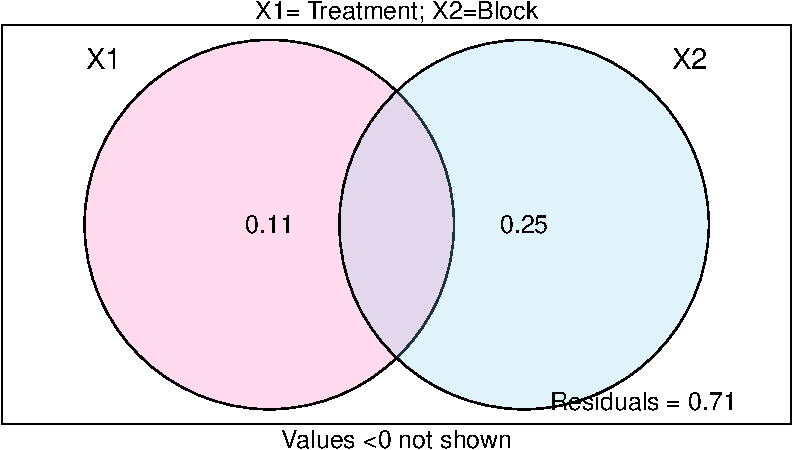
\includegraphics{log-project-aubrie-winnie_files/figure-latex/unnamed-chunk-6-2.pdf}

Composition dissimilarity * 2020 - 2022 *

\begin{Shaded}
\begin{Highlighting}[]
\CommentTok{\# subset data where all t0 communities, insitu log and insitu open communities at t1 and t2 are included.}
\NormalTok{mat3 }\OtherTok{\textless{}{-}}\NormalTok{ mat[}\FunctionTok{which}\NormalTok{(mat}\SpecialCharTok{$}\NormalTok{time}\SpecialCharTok{==}\StringTok{"t0"} \SpecialCharTok{|}\NormalTok{  mat}\SpecialCharTok{$}\NormalTok{treatment}\SpecialCharTok{==}\StringTok{"open"} \SpecialCharTok{|}\NormalTok{ mat}\SpecialCharTok{$}\NormalTok{treatment}\SpecialCharTok{==}\StringTok{"insitu\_log"}\NormalTok{),]}
\NormalTok{mat3}\SpecialCharTok{$}\NormalTok{grp}\OtherTok{\textless{}{-}}\FunctionTok{apply}\NormalTok{(mat3[}\FunctionTok{c}\NormalTok{(}\DecValTok{88}\NormalTok{,}\DecValTok{89}\NormalTok{,}\DecValTok{91}\NormalTok{)], }\DecValTok{1}\NormalTok{, paste, }\AttributeTok{collapse=}\StringTok{":"}\NormalTok{) }\CommentTok{\# block, init as grouping}
\CommentTok{\# names(mat3) \#check}

\CommentTok{\# another df where the grouping variables are time, block and initial state}
\CommentTok{\# each row is a transect in a certain year.}
\NormalTok{df}\OtherTok{\textless{}{-}}\NormalTok{mat3[,}\FunctionTok{c}\NormalTok{(}\DecValTok{1}\SpecialCharTok{:}\DecValTok{87}\NormalTok{, }\DecValTok{93}\NormalTok{)]}
\NormalTok{df2 }\OtherTok{=}\NormalTok{ df }\SpecialCharTok{\%\textgreater{}\%} \FunctionTok{mutate}\NormalTok{(}\FunctionTok{across}\NormalTok{(}\AttributeTok{.cols=}\DecValTok{1}\SpecialCharTok{:}\DecValTok{87}\NormalTok{,}\AttributeTok{.fns=}\NormalTok{as.numeric)) }\CommentTok{\# make everything numeric}
\CommentTok{\# rownames(df2)\textless{}{-}NULL \# remove rownames}

\DocumentationTok{\#\# new with group vars}
\NormalTok{nublock}\OtherTok{\textless{}{-}}\FunctionTok{separate}\NormalTok{(df2, }\DecValTok{88}\NormalTok{, }\FunctionTok{c}\NormalTok{(}\StringTok{"time"}\NormalTok{, }\StringTok{"block"}\NormalTok{, }\StringTok{"init"}\NormalTok{), }\StringTok{":"}\NormalTok{) }\CommentTok{\# just looking at time, block \& initial treatment}

\CommentTok{\# want to sum across transects in same block X init treatment}
\NormalTok{nublock}\SpecialCharTok{$}\NormalTok{sumgrp}\OtherTok{\textless{}{-}}\FunctionTok{apply}\NormalTok{(mat3[}\FunctionTok{c}\NormalTok{(}\DecValTok{88}\NormalTok{,}\DecValTok{89}\NormalTok{, }\DecValTok{91}\NormalTok{)], }\DecValTok{1}\NormalTok{, paste, }\AttributeTok{collapse=}\StringTok{":"}\NormalTok{)}
\CommentTok{\# head(nublock)}

\CommentTok{\# sum observations across initial X  block (group variable)}
\CommentTok{\# this gives number of plants in each transect TYPE for each year in each block. should be 2 types X 3 years X 7 blocks rows }
\NormalTok{blocksum}\OtherTok{\textless{}{-}}\FunctionTok{rowsum}\NormalTok{(nublock[,}\FunctionTok{c}\NormalTok{(}\DecValTok{1}\SpecialCharTok{:}\DecValTok{87}\NormalTok{)], }\AttributeTok{group=}\NormalTok{nublock}\SpecialCharTok{$}\NormalTok{sumgrp)}
\NormalTok{blocksum}\SpecialCharTok{$}\NormalTok{grps}\OtherTok{\textless{}{-}}\FunctionTok{rownames}\NormalTok{(blocksum)}
\FunctionTok{rownames}\NormalTok{(blocksum)}\OtherTok{\textless{}{-}}\ConstantTok{NULL} \CommentTok{\# remove rownames}
\CommentTok{\# nrow(blocksum) \# it is 42 rows as expected }

\DocumentationTok{\#\#  expand again}
\NormalTok{blocksum}\OtherTok{\textless{}{-}}\FunctionTok{separate}\NormalTok{(blocksum, }\DecValTok{88}\NormalTok{, }\FunctionTok{c}\NormalTok{(}\StringTok{"time"}\NormalTok{, }\StringTok{"block"}\NormalTok{, }\StringTok{"init"}\NormalTok{), }\StringTok{":"}\NormalTok{)}

\CommentTok{\# at the moment this includes where there were no plants ("x" column in matrix)}
\NormalTok{assemblies\_t012}\OtherTok{\textless{}{-}}\NormalTok{blocksum[,}\FunctionTok{c}\NormalTok{(}\DecValTok{1}\SpecialCharTok{:}\DecValTok{87}\NormalTok{)]}

\CommentTok{\# group {-} these are the treatment variables that need to be separately fed into the MDS analaysis from the community analysis.}
\NormalTok{group\_init}\OtherTok{\textless{}{-}}\NormalTok{blocksum}\SpecialCharTok{$}\NormalTok{init}
\NormalTok{group\_block}\OtherTok{\textless{}{-}}\NormalTok{blocksum}\SpecialCharTok{$}\NormalTok{block}
\NormalTok{group\_time}\OtherTok{\textless{}{-}}\NormalTok{blocksum}\SpecialCharTok{$}\NormalTok{time}

\CommentTok{\# MDS }
\NormalTok{ass.rel.t012}\OtherTok{\textless{}{-}}\FunctionTok{decostand}\NormalTok{(assemblies\_t012, }\AttributeTok{method=}\StringTok{\textquotesingle{}hel\textquotesingle{}}\NormalTok{) }\CommentTok{\#standardize assemblies }
\NormalTok{ass.rel.t012\_NMS }\OtherTok{\textless{}{-}} \FunctionTok{metaMDS}\NormalTok{(ass.rel.t012, }\AttributeTok{distance =} \StringTok{\textquotesingle{}bray\textquotesingle{}}\NormalTok{, }\AttributeTok{k =} \DecValTok{5}\NormalTok{) }\CommentTok{\# run MDS }
\end{Highlighting}
\end{Shaded}

\begin{verbatim}
## Run 0 stress 0.09244926 
## Run 1 stress 0.09330224 
## Run 2 stress 0.09245033 
## ... Procrustes: rmse 0.0005277273  max resid 0.002067985 
## ... Similar to previous best
## Run 3 stress 0.09244946 
## ... Procrustes: rmse 0.0006846178  max resid 0.002697154 
## ... Similar to previous best
## Run 4 stress 0.09245 
## ... Procrustes: rmse 0.0009709249  max resid 0.003901321 
## ... Similar to previous best
## Run 5 stress 0.09244967 
## ... Procrustes: rmse 0.0002666978  max resid 0.0008037408 
## ... Similar to previous best
## Run 6 stress 0.09244954 
## ... Procrustes: rmse 0.0001738703  max resid 0.0006853886 
## ... Similar to previous best
## Run 7 stress 0.09756596 
## Run 8 stress 0.09245497 
## ... Procrustes: rmse 0.001540151  max resid 0.006173199 
## ... Similar to previous best
## Run 9 stress 0.09244974 
## ... Procrustes: rmse 0.0002972093  max resid 0.001201305 
## ... Similar to previous best
## Run 10 stress 0.09245159 
## ... Procrustes: rmse 0.0008781023  max resid 0.003560637 
## ... Similar to previous best
## Run 11 stress 0.0987328 
## Run 12 stress 0.09244963 
## ... Procrustes: rmse 0.0007775984  max resid 0.003219436 
## ... Similar to previous best
## Run 13 stress 0.0924504 
## ... Procrustes: rmse 0.000515055  max resid 0.002075953 
## ... Similar to previous best
## Run 14 stress 0.09405399 
## Run 15 stress 0.09244959 
## ... Procrustes: rmse 0.0002522251  max resid 0.0006736744 
## ... Similar to previous best
## Run 16 stress 0.09244963 
## ... Procrustes: rmse 0.0008113405  max resid 0.003222829 
## ... Similar to previous best
## Run 17 stress 0.09448663 
## Run 18 stress 0.09246559 
## ... Procrustes: rmse 0.002849452  max resid 0.01117107 
## Run 19 stress 0.09244946 
## ... Procrustes: rmse 0.0001535239  max resid 0.0006064247 
## ... Similar to previous best
## Run 20 stress 0.09244941 
## ... Procrustes: rmse 9.20014e-05  max resid 0.0003035431 
## ... Similar to previous best
## *** Best solution repeated 14 times
\end{verbatim}

\begin{Shaded}
\begin{Highlighting}[]
\CommentTok{\# stressplot(ass.rel.t012\_NMS) \# check fit}

\CommentTok{\# scores}
\NormalTok{mds\_scores\_t012}\OtherTok{\textless{}{-}}\FunctionTok{as.data.frame}\NormalTok{(vegan}\SpecialCharTok{::}\FunctionTok{scores}\NormalTok{(ass.rel.t012\_NMS)}\SpecialCharTok{$}\NormalTok{sites) }\CommentTok{\# extract scores}
\NormalTok{mds\_scores\_t012}\SpecialCharTok{$}\NormalTok{site}\OtherTok{\textless{}{-}}\FunctionTok{rownames}\NormalTok{(vegan}\SpecialCharTok{::}\FunctionTok{scores}\NormalTok{(ass.rel.t012\_NMS)}\SpecialCharTok{$}\NormalTok{sites) }\CommentTok{\# extract names }
\NormalTok{mds\_scores\_t012}\SpecialCharTok{$}\NormalTok{treatment}\OtherTok{\textless{}{-}}\NormalTok{group\_init }\CommentTok{\# grouping factor 1 }
\NormalTok{mds\_scores\_t012}\SpecialCharTok{$}\NormalTok{block}\OtherTok{\textless{}{-}}\NormalTok{group\_block }\CommentTok{\# grouping factor 2 }
\NormalTok{mds\_scores\_t012}\SpecialCharTok{$}\NormalTok{time}\OtherTok{\textless{}{-}}\NormalTok{group\_time }\CommentTok{\# grouping factor 3}

\CommentTok{\# explaining factors}
\NormalTok{init}\OtherTok{\textless{}{-}}\FunctionTok{as.factor}\NormalTok{(group\_init) }\CommentTok{\# grouping factor 1{-} convert to factor}
\NormalTok{block}\OtherTok{\textless{}{-}}\FunctionTok{as.factor}\NormalTok{(group\_block) }\CommentTok{\# grouping factor 2{-} convert to factor}
\NormalTok{time}\OtherTok{\textless{}{-}}\FunctionTok{as.factor}\NormalTok{(group\_time)}

\DocumentationTok{\#\#\#\# rda model analysis \& results \#\#\#\# }
\CommentTok{\# can look at significance of model where initial treatment and block explain variation in community}
\CommentTok{\# trt\_tot\_2\textless{}{-}rda(ass.rel.t012\textasciitilde{}init+block+time) \# run model using standardized data }
\CommentTok{\# summary(trt\_tot\_2)}
\CommentTok{\# anova.cca(trt\_tot\_2, step=1000, by="term") \#\# test for model significance}

\CommentTok{\# can model using varpart to look at contributions of initial treatment and block}
\NormalTok{var.mod2}\OtherTok{\textless{}{-}}\FunctionTok{varpart}\NormalTok{(ass.rel.t012, init, block, time) }\CommentTok{\# run model on standardized data}
\FunctionTok{plot}\NormalTok{(var.mod2, }\AttributeTok{bg=}\FunctionTok{c}\NormalTok{(}\StringTok{"hotpink"}\NormalTok{,}\StringTok{"skyblue"}\NormalTok{,}\StringTok{"lightyellow"}\NormalTok{))}
\FunctionTok{mtext}\NormalTok{(}\StringTok{"X1= Treatment; X2=Block; X3=time"}\NormalTok{, }\AttributeTok{side=}\DecValTok{3}\NormalTok{)}
\end{Highlighting}
\end{Shaded}

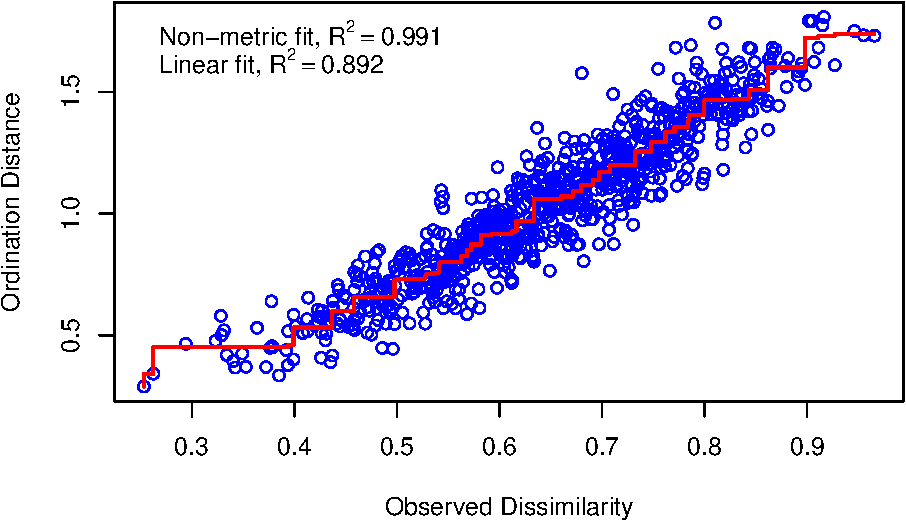
\includegraphics{log-project-aubrie-winnie_files/figure-latex/unnamed-chunk-7-1.pdf}

\begin{Shaded}
\begin{Highlighting}[]
\DocumentationTok{\#\# can test for significance of contribution of the fraction of initial treatment}
\CommentTok{\# do this with partial redundancy analysis}
\NormalTok{trt\_Frac}\OtherTok{\textless{}{-}}\FunctionTok{rda}\NormalTok{(ass.rel.t012}\SpecialCharTok{\textasciitilde{}}\NormalTok{ init }\SpecialCharTok{+}\FunctionTok{Condition}\NormalTok{(block }\SpecialCharTok{+}\NormalTok{ time)) }\CommentTok{\# partial rda model}
\FunctionTok{summary}\NormalTok{(trt\_Frac) }
\end{Highlighting}
\end{Shaded}

\begin{verbatim}
## 
## Call:
## rda(formula = ass.rel.t012 ~ init + Condition(block + time)) 
## 
## Partitioning of variance:
##               Inertia Proportion
## Total         0.56175     1.0000
## Conditioned   0.24900     0.4433
## Constrained   0.03416     0.0608
## Unconstrained 0.27860     0.4959
## 
## Eigenvalues, and their contribution to the variance 
## after removing the contribution of conditiniong variables
## 
## Importance of components:
##                          RDA1    PC1     PC2     PC3     PC4     PC5     PC6
## Eigenvalue            0.03416 0.0397 0.02773 0.02383 0.02008 0.01758 0.01589
## Proportion Explained  0.10921 0.1269 0.08867 0.07618 0.06419 0.05620 0.05080
## Cumulative Proportion 0.10921 0.2362 0.32482 0.40101 0.46520 0.52139 0.57219
##                           PC7     PC8     PC9    PC10    PC11     PC12     PC13
## Eigenvalue            0.01486 0.01326 0.01138 0.01024 0.01004 0.008831 0.008658
## Proportion Explained  0.04752 0.04240 0.03637 0.03273 0.03211 0.028235 0.027685
## Cumulative Proportion 0.61971 0.66211 0.69848 0.73121 0.76332 0.791553 0.819237
##                           PC14     PC15     PC16     PC17     PC18     PC19
## Eigenvalue            0.007353 0.006713 0.005727 0.005255 0.004236 0.003939
## Proportion Explained  0.023511 0.021466 0.018313 0.016802 0.013546 0.012596
## Cumulative Proportion 0.842748 0.864213 0.882526 0.899328 0.912874 0.925469
##                           PC20     PC21     PC22     PC23     PC24     PC25
## Eigenvalue            0.003339 0.003025 0.002930 0.002555 0.002392 0.002270
## Proportion Explained  0.010676 0.009671 0.009367 0.008169 0.007648 0.007257
## Cumulative Proportion 0.936145 0.945816 0.955183 0.963353 0.971001 0.978257
##                           PC26     PC27     PC28      PC29      PC30      PC31
## Eigenvalue            0.001666 0.001540 0.001124 0.0009868 0.0006454 0.0005422
## Proportion Explained  0.005326 0.004923 0.003594 0.0031552 0.0020636 0.0017336
## Cumulative Proportion 0.983583 0.988506 0.992100 0.9952553 0.9973189 0.9990524
##                            PC32
## Eigenvalue            0.0002963
## Proportion Explained  0.0009476
## Cumulative Proportion 1.0000000
## 
## Accumulated constrained eigenvalues
## Importance of components:
##                          RDA1
## Eigenvalue            0.03416
## Proportion Explained  1.00000
## Cumulative Proportion 1.00000
## 
## Scaling 2 for species and site scores
## * Species are scaled proportional to eigenvalues
## * Sites are unscaled: weighted dispersion equal on all dimensions
## * General scaling constant of scores:  2.190697 
## 
## 
## Species scores
## 
##             RDA1        PC1        PC2        PC3        PC4        PC5
## acul   0.0755447 -1.434e-02  7.884e-02 -1.593e-03  8.467e-02  2.948e-02
## aicu   0.0138510 -5.744e-03 -2.254e-02 -3.823e-02 -1.389e-02 -2.313e-02
## arca   0.0000000 -9.271e-18 -2.981e-17 -4.432e-18  1.136e-17 -5.090e-17
## ardy   0.0061606 -3.600e-02  2.215e-02  4.187e-02  7.286e-03 -9.784e-05
## arsp   0.0086051  7.583e-03  1.074e-02  5.817e-03  9.230e-03  2.952e-03
## auel   0.0000000 -4.520e-17 -3.721e-17  1.033e-17  1.268e-17  4.689e-17
## bldr   0.0415582  1.024e-01 -5.538e-02  3.641e-02  6.442e-02 -6.221e-03
## blrd   0.0183399  5.422e-03  2.508e-02  2.563e-03  1.299e-02  1.353e-02
## brdi   0.0119918  9.759e-03  2.022e-03 -2.539e-03  2.480e-03 -4.325e-03
## brdr   0.0000000 -7.790e-18 -1.962e-17  2.861e-17 -4.322e-18 -1.126e-17
## brpe  -0.0548396  5.401e-02 -1.678e-02 -2.939e-02 -2.420e-02 -8.146e-03
## brru   0.0000000  2.293e-17 -1.930e-17 -3.465e-18 -2.242e-17 -2.590e-17
## buse  -0.0161408 -3.475e-03  1.721e-02 -2.478e-04 -3.937e-03  9.186e-03
## caer  -0.0452451 -6.696e-02  9.202e-02 -1.616e-01  4.003e-02 -3.100e-02
## cagr  -0.0551717 -3.321e-02 -1.867e-02 -6.880e-02 -7.224e-02 -3.597e-02
## cahi  -0.0257702 -1.225e-02  5.902e-02  2.155e-02 -1.343e-02 -6.753e-03
## casp   0.0015456 -1.514e-02  8.747e-03  2.929e-02  6.102e-02  1.539e-02
## cear   0.0183399  9.032e-03  3.008e-03  7.984e-03 -3.408e-02 -4.754e-02
## chau   0.0711459  2.373e-02  4.398e-02 -1.230e-01 -5.926e-02 -5.960e-02
## chei   0.0401993  7.383e-03 -2.523e-02  6.336e-03 -3.648e-02  4.773e-02
## chps   0.1934722 -2.173e-02  3.508e-02  7.579e-02  1.279e-01  3.187e-02
## crcl  -0.0071908 -4.839e-02  6.939e-03 -3.034e-02 -3.984e-03  1.194e-03
## crco   0.0909945  1.388e-02  3.934e-02  1.367e-01  3.854e-02 -7.024e-02
## cusc  -0.0215871 -7.383e-02  3.359e-02 -5.510e-02 -1.432e-02  1.409e-02
## cusp   0.0102164 -1.830e-03  2.398e-02 -2.390e-03  8.359e-03  1.051e-02
## dagl  -0.0002086 -1.267e-02 -3.465e-03  4.740e-03  5.809e-03  5.524e-03
## dosp  -0.0228091 -7.269e-02  7.834e-02  1.285e-01 -1.337e-02 -7.897e-02
## ento   0.0000000 -3.969e-18 -6.278e-18 -1.112e-17 -2.983e-19  5.476e-18
## erau  -0.0150169 -3.738e-02  1.412e-02 -2.351e-02 -7.513e-03  8.236e-03
## ercy  -0.0354798 -1.267e-02 -4.291e-02  1.901e-02 -9.685e-03 -3.599e-02
## erra   0.0227357 -1.122e-02  2.726e-02  2.923e-03 -1.143e-02  7.106e-03
## ersp  -0.0084795 -7.754e-03  3.923e-03 -1.604e-03 -1.582e-02  6.429e-03
## gite  -0.0130745  3.665e-02 -9.580e-02 -1.441e-02  6.247e-02  9.662e-03
## gnte   0.0449263  6.207e-03  3.387e-02 -5.636e-02 -6.490e-02 -1.134e-02
## gobe  -0.0389147 -1.221e-02  2.324e-03  2.536e-02  1.356e-02  2.056e-01
## gocy  -0.0005179  3.628e-03  4.776e-02  8.507e-03  3.434e-04 -3.315e-02
## gono   0.0000000  5.463e-18  1.998e-18 -1.741e-18 -8.489e-18  6.585e-19
## goro   0.1287318 -6.246e-02 -1.634e-01  6.953e-02 -2.130e-01  3.958e-02
## gosp   0.0180699  4.609e-03  2.551e-02 -1.270e-02  2.529e-02 -1.785e-02
## haod   0.0085083  2.446e-02  2.793e-03  2.387e-02  5.230e-02 -9.922e-03
## hygl   0.1305498  2.905e-03  1.209e-01  8.285e-02 -5.754e-02  2.925e-02
## hypi  -0.0150169  1.725e-02  4.290e-03 -2.482e-02 -1.172e-02 -1.151e-02
## hypo  -0.0582026 -3.197e-02  8.701e-02  6.189e-02 -2.330e-02  3.009e-02
## jubu   0.0000000  0.000e+00  0.000e+00  0.000e+00  0.000e+00  0.000e+00
## laro  -0.1001787 -5.003e-02  2.308e-02  1.384e-02  3.061e-02 -5.441e-02
## ledu   0.0018314  2.583e-02  1.169e-03  1.944e-02  9.125e-03  1.162e-02
## lele   0.0170846  3.174e-03  7.089e-03  5.462e-03  4.878e-04  1.083e-02
## loef   0.0119918  3.267e-03 -7.624e-04  3.625e-03 -1.161e-02  1.227e-02
## misp  -0.0677312 -9.016e-02  5.996e-02 -1.150e-01 -4.657e-02 -5.294e-02
## mite  -0.0485321  2.148e-01 -5.397e-02 -5.310e-02  3.580e-02  5.387e-02
## momo   0.0000000  0.000e+00  0.000e+00  0.000e+00  0.000e+00  0.000e+00
## mopa   0.0000000  0.000e+00  0.000e+00  0.000e+00  0.000e+00  0.000e+00
## niro  -0.0157499  3.081e-02 -8.896e-03  1.270e-02 -3.637e-03 -2.570e-03
## omco   0.0135532 -9.910e-03 -1.428e-02  4.070e-02 -3.485e-04  1.916e-02
## orsp  -0.0106186 -1.238e-03 -5.492e-03 -1.036e-02  5.195e-05 -5.661e-03
## pala   0.0086051  7.583e-03  1.074e-02  5.817e-03  9.230e-03  2.952e-03
## peai   0.1028116  1.736e-01 -2.005e-01 -3.081e-02  1.369e-02  2.640e-02
## pedu   0.0121694  1.072e-02  1.520e-02  8.226e-03  1.305e-02  4.174e-03
## phsu  -0.0111369  2.179e-02 -6.290e-03  8.980e-03 -2.571e-03 -1.818e-03
## plde   0.0000000  0.000e+00  0.000e+00  0.000e+00  0.000e+00  0.000e+00
## poar   0.0027883 -1.889e-02  1.721e-02 -6.389e-02 -1.656e-02  6.553e-03
## poca   0.0062046  8.808e-02 -6.471e-02 -2.795e-03 -6.767e-02  1.822e-02
## pocap  0.0045075  8.631e-03  3.229e-02 -3.460e-03  2.430e-02  1.976e-02
## poce  -0.0106186 -1.238e-03 -5.492e-03 -1.036e-02  5.195e-05 -5.661e-03
## pogn   0.0000000  0.000e+00  0.000e+00  0.000e+00  0.000e+00  0.000e+00
## pole  -0.0298641  1.578e-01  3.998e-02 -1.008e-01  5.034e-03 -8.070e-03
## pomu   0.1993083 -3.328e-01 -2.100e-01  8.524e-03  8.303e-02 -6.531e-02
## pter   0.0313036 -8.137e-03 -1.022e-02 -6.534e-03  8.000e-03 -2.134e-02
## ptga   0.0518059  6.918e-03  1.242e-01 -6.995e-02 -3.267e-02  1.731e-02
## ptob   0.0000000  0.000e+00  0.000e+00  0.000e+00  0.000e+00  0.000e+00
## rhla  -0.0192925  8.336e-02 -3.393e-02 -1.024e-01  7.481e-02 -1.291e-02
## rhpy  -0.0745613  1.446e-02 -4.187e-02 -1.141e-02 -1.525e-01 -5.915e-02
## rhsp  -0.0241808  1.203e-02  1.080e-01  8.131e-02 -8.713e-02  9.129e-02
## ry     0.0000000  0.000e+00  0.000e+00  0.000e+00  0.000e+00  0.000e+00
## scna   0.0187550  6.243e-03  1.596e-02 -2.118e-02 -3.013e-02 -1.789e-02
## sino  -0.0150169 -3.738e-02  1.412e-02 -2.351e-02 -7.513e-03  8.236e-03
## sool  -0.0138136 -1.380e-02 -7.854e-03  7.919e-03 -7.863e-03 -1.252e-02
## stfi  -0.0194231 -8.594e-03  6.600e-03 -1.169e-02  1.458e-02 -5.568e-03
## stpi   0.0000000  0.000e+00  0.000e+00  0.000e+00  0.000e+00  0.000e+00
## thma   0.0000000  0.000e+00  0.000e+00  0.000e+00  0.000e+00  0.000e+00
## trcy  -0.2242559  2.113e-01  1.067e-02  1.038e-01  8.545e-03 -2.070e-01
## tris   0.0402117 -3.209e-02  1.911e-02 -8.204e-03 -1.746e-02 -5.635e-02
## tror  -0.1544269 -6.830e-02 -3.490e-02 -8.891e-02  5.911e-02  1.022e-02
## trpi  -0.0437537  1.461e-02 -2.404e-02  7.331e-02  2.214e-02  1.813e-03
## waac  -0.1356532 -3.713e-02  4.244e-02 -4.687e-02  6.527e-03 -2.002e-02
## wagr  -0.0065153 -8.588e-03  6.302e-03  2.518e-03  2.094e-03  3.230e-02
## x     -0.0133788 -5.871e-03  2.583e-02 -1.927e-04  4.224e-02  1.243e-03
## 
## 
## Site scores (weighted sums of species scores)
## 
##           RDA1      PC1       PC2        PC3       PC4       PC5
## row1  -0.26449 -0.11731  0.072142 -0.1786127  0.003365 -0.186582
## row2   0.32774 -0.25141 -0.315084 -0.1260442 -0.262245 -0.115106
## row3  -0.46922  0.11517 -0.268870 -0.3406530  0.698008 -0.329868
## row4   0.27897  0.21540 -0.700246 -0.4535292 -0.020427  0.244714
## row5  -0.39084  0.31262 -0.122452  0.2712654 -0.103664 -0.151995
## row6   0.25593  0.23780  0.111247  0.0077685 -0.106470 -0.024464
## row7  -0.28933 -0.30912  0.156394 -0.0639535 -0.630565  0.256295
## row8   0.22871  0.03594  0.165376  0.0061877  0.158766  0.186223
## row9  -0.14623  0.13592 -0.190179  0.4505984 -0.907619  0.085541
## row10  0.63059 -0.41985 -0.221834  0.3855205  0.244325  0.427107
## row11  0.01622 -0.02003  0.033700 -0.0067724  0.106785  0.178492
## row12  0.21309  0.29790  0.422079  0.2285040  0.362588  0.115951
## row13 -0.43323 -0.28242  0.464241 -0.0511444  0.557801  0.003577
## row14  0.04211  0.04939  0.393486 -0.1291351 -0.100648 -0.689887
## row15 -0.20945 -0.53535 -0.191302 -0.4967942  0.149392 -0.088724
## row16  0.48864  0.11795  0.004154  0.4405109  0.555465 -0.021861
## row17 -0.29523  0.06965 -0.199387  0.6302322  0.230438  0.049894
## row18  0.45621  0.06090  0.509639 -0.8875723 -0.461571  0.207254
## row19 -0.49980  0.66131 -0.190927  0.2725541 -0.078050 -0.055167
## row20  0.45815  0.10541  0.194447  0.2727072  0.304887  0.350394
## row21 -0.15821 -0.13366 -0.241084 -0.0026471  0.350202 -0.173006
## row22  0.08433  0.09447  0.730090 -0.1782412  0.173954  0.148209
## row23 -0.87372  0.38836  0.096577 -0.5587161 -0.263845 -0.259079
## row24  0.54389 -0.30905 -0.033889  0.1578082  0.214942  0.339469
## row25 -0.19692 -0.33779 -0.192198  0.1937864 -0.192412 -0.306358
## row26  0.31799 -0.17579 -0.145749 -0.0141532 -0.348512  0.314036
## row27 -0.30510 -0.17289 -0.395816  0.0233742 -0.006757  0.371098
## row28  0.18924  0.16647  0.055446  0.1471508 -0.628134 -0.876158
## row29 -0.59762  0.26775  0.658661  0.2113891 -0.436792  0.732128
## row30  0.25517  0.51838 -0.228572  0.1495511 -0.009184 -0.319855
## row31 -0.23382 -0.55322  0.680356  0.9493292 -0.119289 -0.517903
## row32  0.26309  0.09208 -0.021492  0.1021932 -0.327159  0.345909
## row33 -0.22411 -0.84145  0.317819 -0.5291453 -0.169109  0.185397
## row34  0.40068 -0.47569 -0.310134 -0.2951499  0.152405 -0.304166
## row35 -0.26668  0.40753 -0.725183  0.0061752 -0.074115 -0.128422
## row36  0.40119 -0.09516 -0.085593  0.2324789  0.021757 -0.289300
## row37 -0.68266  0.77489  0.513757 -0.4592464  0.421879 -0.215783
## row38  0.52814 -0.57026 -0.164432  0.0240354  0.290319 -0.377254
## row39 -0.49625 -0.03940 -0.174828 -0.3297816  0.001654 -0.180206
## row40  0.14586  0.27510  0.056997 -0.0715832  0.069898 -0.121915
## row41 -0.08197  0.20944 -0.101421  0.0087625  0.462695  0.730672
## row42  0.58896  0.03001 -0.415936  0.0009919 -0.284957  0.460698
## 
## 
## Site constraints (linear combinations of constraining variables)
## 
##         RDA1      PC1       PC2        PC3       PC4       PC5
## row1  -0.338 -0.11731  0.072142 -0.1786127  0.003365 -0.186582
## row2   0.338 -0.25141 -0.315084 -0.1260442 -0.262245 -0.115106
## row3  -0.338  0.11517 -0.268870 -0.3406530  0.698008 -0.329868
## row4   0.338  0.21540 -0.700246 -0.4535292 -0.020427  0.244714
## row5  -0.338  0.31262 -0.122452  0.2712654 -0.103664 -0.151995
## row6   0.338  0.23780  0.111247  0.0077685 -0.106470 -0.024464
## row7  -0.338 -0.30912  0.156394 -0.0639535 -0.630565  0.256295
## row8   0.338  0.03594  0.165376  0.0061877  0.158766  0.186223
## row9  -0.338  0.13592 -0.190179  0.4505984 -0.907619  0.085541
## row10  0.338 -0.41985 -0.221834  0.3855205  0.244325  0.427107
## row11 -0.338 -0.02003  0.033700 -0.0067724  0.106785  0.178492
## row12  0.338  0.29790  0.422079  0.2285040  0.362588  0.115951
## row13 -0.338 -0.28242  0.464241 -0.0511444  0.557801  0.003577
## row14  0.338  0.04939  0.393486 -0.1291351 -0.100648 -0.689887
## row15 -0.338 -0.53535 -0.191302 -0.4967942  0.149392 -0.088724
## row16  0.338  0.11795  0.004154  0.4405109  0.555465 -0.021861
## row17 -0.338  0.06965 -0.199387  0.6302322  0.230438  0.049894
## row18  0.338  0.06090  0.509639 -0.8875723 -0.461571  0.207254
## row19 -0.338  0.66131 -0.190927  0.2725541 -0.078050 -0.055167
## row20  0.338  0.10541  0.194447  0.2727072  0.304887  0.350394
## row21 -0.338 -0.13366 -0.241084 -0.0026471  0.350202 -0.173006
## row22  0.338  0.09447  0.730090 -0.1782412  0.173954  0.148209
## row23 -0.338  0.38836  0.096577 -0.5587161 -0.263845 -0.259079
## row24  0.338 -0.30905 -0.033889  0.1578082  0.214942  0.339469
## row25 -0.338 -0.33779 -0.192198  0.1937864 -0.192412 -0.306358
## row26  0.338 -0.17579 -0.145749 -0.0141532 -0.348512  0.314036
## row27 -0.338 -0.17289 -0.395816  0.0233742 -0.006757  0.371098
## row28  0.338  0.16647  0.055446  0.1471508 -0.628134 -0.876158
## row29 -0.338  0.26775  0.658661  0.2113891 -0.436792  0.732128
## row30  0.338  0.51838 -0.228572  0.1495511 -0.009184 -0.319855
## row31 -0.338 -0.55322  0.680356  0.9493292 -0.119289 -0.517903
## row32  0.338  0.09208 -0.021492  0.1021932 -0.327159  0.345909
## row33 -0.338 -0.84145  0.317819 -0.5291453 -0.169109  0.185397
## row34  0.338 -0.47569 -0.310134 -0.2951499  0.152405 -0.304166
## row35 -0.338  0.40753 -0.725183  0.0061752 -0.074115 -0.128422
## row36  0.338 -0.09516 -0.085593  0.2324789  0.021757 -0.289300
## row37 -0.338  0.77489  0.513757 -0.4592464  0.421879 -0.215783
## row38  0.338 -0.57026 -0.164432  0.0240354  0.290319 -0.377254
## row39 -0.338 -0.03940 -0.174828 -0.3297816  0.001654 -0.180206
## row40  0.338  0.27510  0.056997 -0.0715832  0.069898 -0.121915
## row41 -0.338  0.20944 -0.101421  0.0087625  0.462695  0.730672
## row42  0.338  0.03001 -0.415936  0.0009919 -0.284957  0.460698
## 
## 
## Biplot scores for constraining variables
## 
##          RDA1 PC1 PC2 PC3 PC4 PC5
## initopen    1   0   0   0   0   0
## 
## 
## Centroids for factor constraints
## 
##            RDA1 PC1 PC2 PC3 PC4 PC5
## initlog  -0.338   0   0   0   0   0
## initopen  0.338   0   0   0   0   0
\end{verbatim}

\begin{Shaded}
\begin{Highlighting}[]
\FunctionTok{RsquareAdj}\NormalTok{(trt\_Frac)}\SpecialCharTok{$}\NormalTok{adj.r.squared }\CommentTok{\#explanatory power}
\end{Highlighting}
\end{Shaded}

\begin{verbatim}
## [1] 0.05628909
\end{verbatim}

\begin{Shaded}
\begin{Highlighting}[]
\FunctionTok{anova.cca}\NormalTok{(trt\_Frac) }\DocumentationTok{\#\# this tells us if first condition, init, significantly contributes to overall variance explanation. }
\end{Highlighting}
\end{Shaded}

\begin{verbatim}
## Permutation test for rda under reduced model
## Permutation: free
## Number of permutations: 999
## 
## Model: rda(formula = ass.rel.t012 ~ init + Condition(block + time))
##          Df Variance      F Pr(>F)    
## Model     1 0.034157 3.9233  0.001 ***
## Residual 32 0.278596                  
## ---
## Signif. codes:  0 '***' 0.001 '**' 0.01 '*' 0.05 '.' 0.1 ' ' 1
\end{verbatim}

\begin{Shaded}
\begin{Highlighting}[]
\DocumentationTok{\#\#\# extracting species scores and plotting }
\CommentTok{\# species scores}
\NormalTok{species.scores}\OtherTok{\textless{}{-}}\FunctionTok{as.data.frame}\NormalTok{(vegan}\SpecialCharTok{::}\FunctionTok{scores}\NormalTok{(ass.rel.t012\_NMS,}\StringTok{"species"}\NormalTok{)) }\DocumentationTok{\#\# some species don\textquotesingle{}t have scores}
\NormalTok{species.scores}\SpecialCharTok{$}\NormalTok{species}\OtherTok{\textless{}{-}}\FunctionTok{rownames}\NormalTok{(species.scores) }

\DocumentationTok{\#\#\# NMDS 1 and 2 }
\NormalTok{log}\OtherTok{\textless{}{-}}\NormalTok{mds\_scores\_t012[mds\_scores\_t012}\SpecialCharTok{$}\NormalTok{treatment }\SpecialCharTok{==} \StringTok{"log"}\NormalTok{, ][}\FunctionTok{chull}\NormalTok{(mds\_scores\_t012[mds\_scores\_t012}\SpecialCharTok{$}\NormalTok{treatment }\SpecialCharTok{==} 
                                                          \StringTok{"log"}\NormalTok{, }\FunctionTok{c}\NormalTok{(}\StringTok{"NMDS1"}\NormalTok{, }\StringTok{"NMDS2"}\NormalTok{)]), ]}

\NormalTok{open}\OtherTok{\textless{}{-}}\NormalTok{mds\_scores\_t012[mds\_scores\_t012}\SpecialCharTok{$}\NormalTok{treatment }\SpecialCharTok{==} \StringTok{"open"}\NormalTok{, ][}\FunctionTok{chull}\NormalTok{(mds\_scores\_t012[mds\_scores\_t012}\SpecialCharTok{$}\NormalTok{treatment }\SpecialCharTok{==} 
                                                               \StringTok{"open"}\NormalTok{, }\FunctionTok{c}\NormalTok{(}\StringTok{"NMDS1"}\NormalTok{, }\StringTok{"NMDS2"}\NormalTok{)]), ]}

\NormalTok{hulldat}\OtherTok{\textless{}{-}}\FunctionTok{rbind}\NormalTok{(log,open)}

\FunctionTok{options}\NormalTok{(}\AttributeTok{ggrepel.max.overlaps =} \ConstantTok{Inf}\NormalTok{)}
\NormalTok{nmds.plot }\OtherTok{\textless{}{-}} \FunctionTok{ggplot}\NormalTok{()}\SpecialCharTok{+}
  \FunctionTok{theme\_bw}\NormalTok{()}\SpecialCharTok{+}
  \FunctionTok{theme}\NormalTok{(}\AttributeTok{panel.background =} \FunctionTok{element\_blank}\NormalTok{(),}
        \AttributeTok{panel.grid.major =} \FunctionTok{element\_blank}\NormalTok{(),  }\CommentTok{\#remove major{-}grid labels}
        \AttributeTok{panel.grid.minor =} \FunctionTok{element\_blank}\NormalTok{(),  }\CommentTok{\#remove minor{-}grid labels}
        \AttributeTok{plot.background =} \FunctionTok{element\_blank}\NormalTok{(), }
        \AttributeTok{axis.text =} \FunctionTok{element\_text}\NormalTok{(}\AttributeTok{size =} \DecValTok{15}\NormalTok{),}
        \AttributeTok{axis.title=}\FunctionTok{element\_text}\NormalTok{(}\AttributeTok{size=}\DecValTok{20}\NormalTok{),}
        \AttributeTok{legend.title=}\FunctionTok{element\_text}\NormalTok{(}\AttributeTok{size=}\DecValTok{20}\NormalTok{), }
        \AttributeTok{legend.text=}\FunctionTok{element\_text}\NormalTok{(}\AttributeTok{size=}\DecValTok{15}\NormalTok{))}\SpecialCharTok{+}
  \FunctionTok{geom\_text\_repel}\NormalTok{(}\AttributeTok{data=}\NormalTok{species.scores, }\FunctionTok{aes}\NormalTok{(NMDS1, NMDS2, }\AttributeTok{label=}\NormalTok{species), }\AttributeTok{alpha=}\FloatTok{0.9}\NormalTok{, }\AttributeTok{size=}\DecValTok{5}\NormalTok{, }\AttributeTok{col=}\StringTok{\textquotesingle{}darkgray\textquotesingle{}}\NormalTok{,}\AttributeTok{na.rm=}\ConstantTok{TRUE}\NormalTok{)}\SpecialCharTok{+}
  \FunctionTok{geom\_polygon}\NormalTok{(}\AttributeTok{data=}\NormalTok{hulldat, }\FunctionTok{aes}\NormalTok{(NMDS1, NMDS2, }\AttributeTok{fill=}\NormalTok{treatment, }\AttributeTok{group=}\NormalTok{treatment), }\AttributeTok{alpha=}\FloatTok{0.3}\NormalTok{)}\SpecialCharTok{+}\FunctionTok{scale\_fill\_manual}\NormalTok{(}\AttributeTok{values=}\FunctionTok{c}\NormalTok{(}\StringTok{"\#63A088"}\NormalTok{,}\StringTok{"\#56638A"}\NormalTok{), }\AttributeTok{name=}\StringTok{"Treatment"}\NormalTok{)}\SpecialCharTok{+}
  \FunctionTok{geom\_point}\NormalTok{(}\AttributeTok{data=}\NormalTok{mds\_scores\_t012, }\FunctionTok{aes}\NormalTok{(NMDS1, NMDS2, }\AttributeTok{shape=}\NormalTok{block, }\AttributeTok{col=}\NormalTok{treatment), }\AttributeTok{size=}\DecValTok{6}\NormalTok{)}\SpecialCharTok{+} \FunctionTok{scale\_shape\_manual}\NormalTok{(}\AttributeTok{values =} \FunctionTok{c}\NormalTok{(}\DecValTok{14}\NormalTok{,}\DecValTok{15}\NormalTok{,}\DecValTok{16}\NormalTok{,}\DecValTok{17}\NormalTok{,}\DecValTok{11}\NormalTok{,}\DecValTok{18}\NormalTok{,}\DecValTok{8}\NormalTok{), }\AttributeTok{name=}\StringTok{\textquotesingle{}Block\textquotesingle{}}\NormalTok{)}\SpecialCharTok{+}
  \FunctionTok{scale\_colour\_manual}\NormalTok{(}\AttributeTok{values=}\FunctionTok{c}\NormalTok{(}\StringTok{"\#63A088"}\NormalTok{,}\StringTok{"\#56638A"}\NormalTok{), }\AttributeTok{name=}\StringTok{"Treatment"}\NormalTok{) }\SpecialCharTok{+}
  \FunctionTok{labs}\NormalTok{(}\AttributeTok{title=}\FunctionTok{paste0}\NormalTok{(}\StringTok{"Stress: "}\NormalTok{, }\FunctionTok{round}\NormalTok{(ass.rel.t012\_NMS}\SpecialCharTok{$}\NormalTok{stress,}\DecValTok{3}\NormalTok{)))}
 
\FunctionTok{print}\NormalTok{(nmds.plot)}
\end{Highlighting}
\end{Shaded}

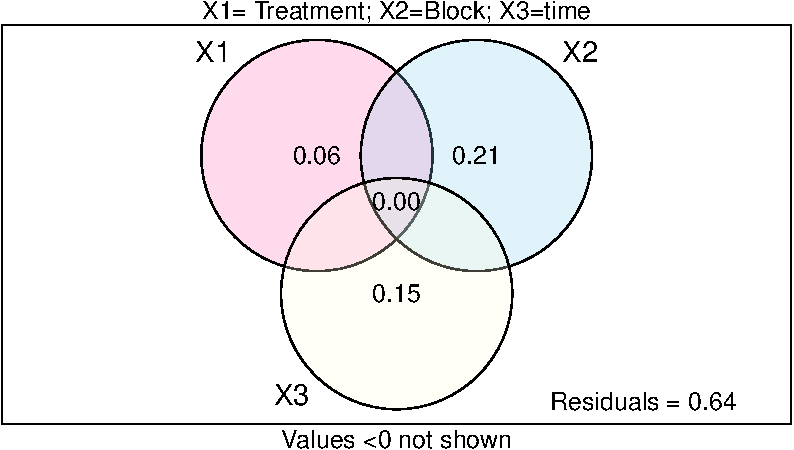
\includegraphics{log-project-aubrie-winnie_files/figure-latex/unnamed-chunk-7-2.pdf}

\begin{Shaded}
\begin{Highlighting}[]
\CommentTok{\# All other NMDS pairs}
\NormalTok{treatments }\OtherTok{\textless{}{-}} \FunctionTok{unique}\NormalTok{(mds\_scores\_t012}\SpecialCharTok{$}\NormalTok{treatment)}
\NormalTok{plots }\OtherTok{\textless{}{-}} \FunctionTok{list}\NormalTok{()}
\NormalTok{num\_axes }\OtherTok{\textless{}{-}} \DecValTok{5}  

\ControlFlowTok{for}\NormalTok{ (i }\ControlFlowTok{in} \DecValTok{1}\SpecialCharTok{:}\NormalTok{num\_axes) \{}
  \ControlFlowTok{for}\NormalTok{ (j }\ControlFlowTok{in}\NormalTok{ (i}\SpecialCharTok{+}\DecValTok{1}\NormalTok{)}\SpecialCharTok{:}\NormalTok{num\_axes) \{  }
    \ControlFlowTok{if}\NormalTok{ (j }\SpecialCharTok{\textless{}=}\NormalTok{ num\_axes }\SpecialCharTok{\&\&}\NormalTok{ i }\SpecialCharTok{!=}\NormalTok{ j) \{  }
\NormalTok{      log }\OtherTok{\textless{}{-}}\NormalTok{ mds\_scores\_t012[mds\_scores\_t012}\SpecialCharTok{$}\NormalTok{treatment }\SpecialCharTok{==} \StringTok{"log"}\NormalTok{, ]}
\NormalTok{      open }\OtherTok{\textless{}{-}}\NormalTok{ mds\_scores\_t012[mds\_scores\_t012}\SpecialCharTok{$}\NormalTok{treatment }\SpecialCharTok{==} \StringTok{"open"}\NormalTok{, ]}
      
\NormalTok{      log\_hull }\OtherTok{\textless{}{-}}\NormalTok{ log[}\FunctionTok{chull}\NormalTok{(log[[}\FunctionTok{paste0}\NormalTok{(}\StringTok{"NMDS"}\NormalTok{, i)]], log[[}\FunctionTok{paste0}\NormalTok{(}\StringTok{"NMDS"}\NormalTok{, j)]]), ]}
\NormalTok{      open\_hull }\OtherTok{\textless{}{-}}\NormalTok{ open[}\FunctionTok{chull}\NormalTok{(open[[}\FunctionTok{paste0}\NormalTok{(}\StringTok{"NMDS"}\NormalTok{, i)]], open[[}\FunctionTok{paste0}\NormalTok{(}\StringTok{"NMDS"}\NormalTok{, j)]]), ]}
      
\NormalTok{      hulldat }\OtherTok{\textless{}{-}} \FunctionTok{rbind}\NormalTok{(log\_hull, open\_hull)}
      
\NormalTok{      plot\_name }\OtherTok{\textless{}{-}} \FunctionTok{paste0}\NormalTok{(i, }\StringTok{"+"}\NormalTok{, j)}
      
\NormalTok{      plots[[plot\_name]] }\OtherTok{\textless{}{-}} \FunctionTok{ggplot}\NormalTok{() }\SpecialCharTok{+}
        \FunctionTok{theme\_bw}\NormalTok{() }\SpecialCharTok{+}
        \FunctionTok{theme}\NormalTok{(}\AttributeTok{panel.background =} \FunctionTok{element\_blank}\NormalTok{(),}
              \AttributeTok{panel.grid.major =} \FunctionTok{element\_blank}\NormalTok{(),}
              \AttributeTok{panel.grid.minor =} \FunctionTok{element\_blank}\NormalTok{(),}
              \AttributeTok{plot.background =} \FunctionTok{element\_blank}\NormalTok{(),}
              \AttributeTok{axis.text =} \FunctionTok{element\_text}\NormalTok{(}\AttributeTok{size =} \DecValTok{15}\NormalTok{),}
              \AttributeTok{axis.title =} \FunctionTok{element\_text}\NormalTok{(}\AttributeTok{size =} \DecValTok{15}\NormalTok{),}
              \AttributeTok{legend.title =} \FunctionTok{element\_text}\NormalTok{(}\AttributeTok{size =} \DecValTok{15}\NormalTok{),}
              \AttributeTok{legend.text =} \FunctionTok{element\_text}\NormalTok{(}\AttributeTok{size =} \DecValTok{10}\NormalTok{)) }\SpecialCharTok{+}
        \FunctionTok{geom\_text\_repel}\NormalTok{(}\AttributeTok{data =}\NormalTok{ species.scores, }\FunctionTok{aes}\NormalTok{(}\AttributeTok{x =} \SpecialCharTok{!!}\FunctionTok{sym}\NormalTok{(}\FunctionTok{paste0}\NormalTok{(}\StringTok{"NMDS"}\NormalTok{, i)), }\AttributeTok{y =} \SpecialCharTok{!!}\FunctionTok{sym}\NormalTok{(}\FunctionTok{paste0}\NormalTok{(}\StringTok{"NMDS"}\NormalTok{, j)), }\AttributeTok{label =}\NormalTok{ species), }\AttributeTok{alpha =} \FloatTok{0.9}\NormalTok{, }\AttributeTok{size =} \DecValTok{3}\NormalTok{, }\AttributeTok{col =} \StringTok{\textquotesingle{}darkgray\textquotesingle{}}\NormalTok{, }\AttributeTok{na.rm =} \ConstantTok{TRUE}\NormalTok{) }\SpecialCharTok{+}
        \FunctionTok{geom\_polygon}\NormalTok{(}\AttributeTok{data =}\NormalTok{ hulldat, }\FunctionTok{aes}\NormalTok{(}\AttributeTok{x =} \SpecialCharTok{!!}\FunctionTok{sym}\NormalTok{(}\FunctionTok{paste0}\NormalTok{(}\StringTok{"NMDS"}\NormalTok{, i)), }\AttributeTok{y =} \SpecialCharTok{!!}\FunctionTok{sym}\NormalTok{(}\FunctionTok{paste0}\NormalTok{(}\StringTok{"NMDS"}\NormalTok{, j)), }\AttributeTok{fill =}\NormalTok{ treatment, }\AttributeTok{group =}\NormalTok{ treatment), }\AttributeTok{alpha =} \FloatTok{0.3}\NormalTok{) }\SpecialCharTok{+} 
        \FunctionTok{scale\_fill\_manual}\NormalTok{(}\AttributeTok{values =} \FunctionTok{c}\NormalTok{(}\StringTok{"\#63A088"}\NormalTok{, }\StringTok{"\#56638A"}\NormalTok{), }\AttributeTok{name =} \StringTok{"Treatment"}\NormalTok{) }\SpecialCharTok{+}
        \FunctionTok{geom\_point}\NormalTok{(}\AttributeTok{data =}\NormalTok{ mds\_scores\_t012, }\FunctionTok{aes}\NormalTok{(}\AttributeTok{x =} \SpecialCharTok{!!}\FunctionTok{sym}\NormalTok{(}\FunctionTok{paste0}\NormalTok{(}\StringTok{"NMDS"}\NormalTok{, i)), }\AttributeTok{y =} \SpecialCharTok{!!}\FunctionTok{sym}\NormalTok{(}\FunctionTok{paste0}\NormalTok{(}\StringTok{"NMDS"}\NormalTok{, j)), }\AttributeTok{shape =}\NormalTok{ block, }\AttributeTok{col =}\NormalTok{ treatment), }\AttributeTok{size =} \DecValTok{6}\NormalTok{) }\SpecialCharTok{+} \FunctionTok{scale\_shape\_manual}\NormalTok{(}\AttributeTok{values =} \FunctionTok{c}\NormalTok{(}\DecValTok{14}\NormalTok{, }\DecValTok{15}\NormalTok{, }\DecValTok{16}\NormalTok{, }\DecValTok{17}\NormalTok{, }\DecValTok{11}\NormalTok{, }\DecValTok{18}\NormalTok{, }\DecValTok{8}\NormalTok{), }\AttributeTok{name =} \StringTok{\textquotesingle{}Block\textquotesingle{}}\NormalTok{) }\SpecialCharTok{+}
        \FunctionTok{scale\_colour\_manual}\NormalTok{(}\AttributeTok{values =} \FunctionTok{c}\NormalTok{(}\StringTok{"\#63A088"}\NormalTok{, }\StringTok{"\#56638A"}\NormalTok{), }\AttributeTok{name =} \StringTok{"Treatment"}\NormalTok{) }\SpecialCharTok{+}
        \FunctionTok{xlab}\NormalTok{(}\FunctionTok{paste0}\NormalTok{(}\StringTok{"NMDS"}\NormalTok{, i)) }\SpecialCharTok{+}
        \FunctionTok{ylab}\NormalTok{(}\FunctionTok{paste0}\NormalTok{(}\StringTok{"NMDS"}\NormalTok{, j))}
\NormalTok{    \}}
\NormalTok{  \}}
\NormalTok{\}}


\NormalTok{((plots}\SpecialCharTok{$}\StringTok{\textasciigrave{}}\AttributeTok{1+3}\StringTok{\textasciigrave{}} \SpecialCharTok{+}\NormalTok{ plots}\SpecialCharTok{$}\StringTok{\textasciigrave{}}\AttributeTok{1+4}\StringTok{\textasciigrave{}}\SpecialCharTok{+}\NormalTok{ plots}\SpecialCharTok{$}\StringTok{\textasciigrave{}}\AttributeTok{1+5}\StringTok{\textasciigrave{}}\NormalTok{)}\SpecialCharTok{/}\NormalTok{(plots}\SpecialCharTok{$}\StringTok{\textasciigrave{}}\AttributeTok{2+3}\StringTok{\textasciigrave{}} \SpecialCharTok{+}\NormalTok{ plots}\SpecialCharTok{$}\StringTok{\textasciigrave{}}\AttributeTok{2+4}\StringTok{\textasciigrave{}}\SpecialCharTok{+}\NormalTok{ plots}\SpecialCharTok{$}\StringTok{\textasciigrave{}}\AttributeTok{2+5}\StringTok{\textasciigrave{}}\NormalTok{)}\SpecialCharTok{/}\NormalTok{(plots}\SpecialCharTok{$}\StringTok{\textasciigrave{}}\AttributeTok{3+4}\StringTok{\textasciigrave{}} \SpecialCharTok{+}\NormalTok{ plots}\SpecialCharTok{$}\StringTok{\textasciigrave{}}\AttributeTok{3+5}\StringTok{\textasciigrave{}}\SpecialCharTok{+}\NormalTok{ plots}\SpecialCharTok{$}\StringTok{\textasciigrave{}}\AttributeTok{4+5}\StringTok{\textasciigrave{}}\NormalTok{)) }\SpecialCharTok{+} \FunctionTok{plot\_layout}\NormalTok{(}\AttributeTok{guides =}\StringTok{"collect"}\NormalTok{) }\SpecialCharTok{+} \FunctionTok{plot\_annotation}\NormalTok{(}\FunctionTok{paste0}\NormalTok{(}\StringTok{"Stress:"}\NormalTok{,}\FunctionTok{round}\NormalTok{(ass.rel.t012\_NMS}\SpecialCharTok{$}\NormalTok{stress,}\DecValTok{3}\NormalTok{), }\StringTok{" (k = 5)"}\NormalTok{))}
\end{Highlighting}
\end{Shaded}

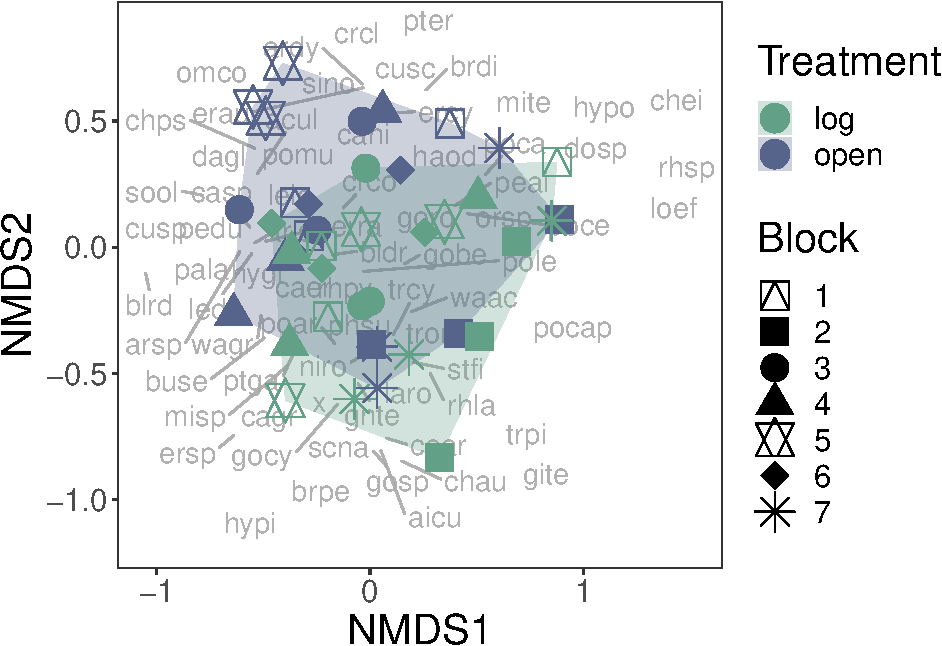
\includegraphics{log-project-aubrie-winnie_files/figure-latex/unnamed-chunk-7-3.pdf}

\hypertarget{q2-why-are-plant-communities-in-fallen-log-patches-different-from-patches-in-the-open}{%
\subsubsection{\texorpdfstring{\textbf{Q2 Why are plant communities in
fallen log patches different from patches in the
open?}}{Q2 Why are plant communities in fallen log patches different from patches in the open? }}\label{q2-why-are-plant-communities-in-fallen-log-patches-different-from-patches-in-the-open}}

\hypertarget{overview-of-results-1}{%
\paragraph{\texorpdfstring{\emph{Overview of results}
}{Overview of results  }}\label{overview-of-results-1}}

\emph{Nutrient comparison} Total soil carbon is significantly higher in
log patches than open patches (Wilcoxon rank sum test, p\textless0.05).

\emph{2020-2022} There are three response variables: count (Poisson),
Shannon diversity index (hurdle: binomial and Gaussian), and composition
matrix. 1. \emph{Abundance} -- the inclusive model includes all nutrient
elements as additive fixed factors with block and year as random terms.
As suggested by this inclusive model, the abundance of plants is
significantly more likely to increase with soil carbon (C: p=0.004)
level but decrease with plant-available nitrogen (NH4N: p\textless0.001)
and basic exchangeable cations (CEC: p=0.008). {[}This seems to be a bit
confounding as it does not make sense biologically. Maybe an artefact of
collinearity?{]} 2. \emph{Diversity} -- the probability of having a
positive Shannon diversity index in the plant community is significantly
higher with higher levels of plant-available nitrogen (NO3N: p
\textless{} 0.05) and potassium (K: p \textless{} 0.05) but lower with
higher soil phosphorus (P: p \textless0.05). A similar pattern is
observed for the level of diversity. The presented model has a structure
of ``diversity \textasciitilde{} elements (additive) + (1\textbar block)
+ (1\textbar year)''. 3. \emph{Composition} -- The composition of plant
communities is not significantly explained by any of the nutrient
elements. See print(en.nutrient).

\emph{2020} There are three response variables: count (Poisson), Shannon
diversity index (hurdle: binomial and Gaussian), and composition matrix.
1. \emph{Abundance} -- the inclusive model includes all nutrient
elements as additive fixed factors with block and year as random terms.
As suggested by this inclusive model, the abundance of plants is
significantly more likely to increase with soil carbon (C: p=0.04)
level. 2. \emph{Diversity} -- the probability of having a positive
Shannon diversity index in the plant community is significantly higher
with higher levels of plant-available nitrogen (NO3N: p \textless{}
0.05) and potassium (K: p \textless{} 0.05). A similar pattern is
observed for the level of diversity. The presented model has a structure
of ``diversity \textasciitilde{} elements (additive) +
(1\textbar block)''. 3. \emph{Composition} -- The composition of plant
communities is not significantly explained by any of the nutrient
elements. See print(en.nutrient).

\emph{2021} There are three response variables: count (Poisson), Shannon
diversity index (hurdle: binomial and Gaussian), and composition matrix.
1. \emph{Abundance} -- the inclusive model includes all nutrient
elements as additive fixed factors with block and year as random terms.
As suggested by this inclusive model, the abundance of plants is
significantly more likely to increase with plant-available phosphorus
(P: p=0.03) level but decrease with plant-available nitrogen (NH4N:
p=0.009). {[}Same comment{]} 2. \emph{Diversity} -- the level of plant
diversity as represented by the Shannon diversity index and the
probability of having a positive Shannon diversity index in the plant
community are not significantly explained by any soil nutrient elements.
The presented model has a structure of ``diversity \textasciitilde{}
elements (additive) + (1\textbar block)''. 3. \emph{Composition} -- The
composition of plant communities is not significantly explained by any
of the nutrient elements. See print(en.nutrient).

\emph{2022} There are three response variables: count (Poisson), Shannon
diversity index (hurdle: binomial and Gaussian), and composition matrix.
1. \emph{Abundance} -- the inclusive model includes all nutrient
elements as additive fixed factors with block and year as random terms.
As suggested by this inclusive model, the abundance of plants is
significantly more likely to decrease with plant-available nitrogen
(NH4N: p\textless0.001) and potassium (K: p=0.03). {[}Same comment{]} 2.
\emph{Diversity} -- the level of plant diversity as represented by the
Shannon diversity index and the probability of having a positive Shannon
diversity index in the plant community are not significantly explained
by any soil nutrient elements. The presented model has a structure of
``diversity \textasciitilde{} elements (additive) + (1\textbar block)''.
3. \emph{Composition} -- The composition of plant communities is not
significantly explained by any of the nutrient elements. See
print(en.nutrient).

\hypertarget{statistical-methods-1}{%
\paragraph{\texorpdfstring{\emph{Statistical Methods}
}{Statistical Methods  }}\label{statistical-methods-1}}

\hypertarget{analysis-1}{%
\paragraph{\texorpdfstring{\emph{Analysis}}{Analysis }}\label{analysis-1}}

\begin{itemize}
\tightlist
\item
  nutrient analysis (nutrient composition \textasciitilde{} log vs open;
  abundance \textasciitilde{} nutrient composition , diversity
  \textasciitilde{} nutrient composition, composition \textasciitilde{}
  nutrient composition)
\end{itemize}

\begin{Shaded}
\begin{Highlighting}[]
\FunctionTok{library}\NormalTok{(ggplot2)}
\FunctionTok{library}\NormalTok{(ggpubr)}
\FunctionTok{library}\NormalTok{(dplyr)}
\FunctionTok{library}\NormalTok{(lme4)}
\FunctionTok{library}\NormalTok{(emmeans)}
\FunctionTok{library}\NormalTok{(pscl)}
\end{Highlighting}
\end{Shaded}

\begin{verbatim}
## Classes and Methods for R originally developed in the
## Political Science Computational Laboratory
## Department of Political Science
## Stanford University (2002-2015),
## by and under the direction of Simon Jackman.
## hurdle and zeroinfl functions by Achim Zeileis.
\end{verbatim}

\begin{Shaded}
\begin{Highlighting}[]
\FunctionTok{library}\NormalTok{(glmmTMB)}
\end{Highlighting}
\end{Shaded}

\begin{verbatim}
## Warning in checkDepPackageVersion(dep_pkg = "TMB"): Package version inconsistency detected.
## glmmTMB was built with TMB version 1.9.6
## Current TMB version is 1.9.10
## Please re-install glmmTMB from source or restore original 'TMB' package (see '?reinstalling' for more information)
\end{verbatim}

\begin{Shaded}
\begin{Highlighting}[]
\FunctionTok{library}\NormalTok{(tidyr)}
\FunctionTok{library}\NormalTok{(DHARMa)}
\FunctionTok{library}\NormalTok{(ggplot2)}
\FunctionTok{library}\NormalTok{(AICcmodavg)}
\end{Highlighting}
\end{Shaded}

\begin{verbatim}
## 
## Attaching package: 'AICcmodavg'
\end{verbatim}

\begin{verbatim}
## The following object is masked from 'package:lme4':
## 
##     checkConv
\end{verbatim}

\begin{verbatim}
## The following object is masked from 'package:labdsv':
## 
##     importance
\end{verbatim}

\begin{Shaded}
\begin{Highlighting}[]
\FunctionTok{library}\NormalTok{(ggpubr)}

\CommentTok{\# Set up nutrient analysis data}
\NormalTok{nutrient }\OtherTok{\textless{}{-}} \FunctionTok{read.csv}\NormalTok{(}\StringTok{"Nutrient.csv"}\NormalTok{, }\AttributeTok{header =}\NormalTok{ T)}
\NormalTok{nutrient }\OtherTok{\textless{}{-}}\FunctionTok{separate}\NormalTok{(nutrient,}\DecValTok{2}\NormalTok{ , }\FunctionTok{c}\NormalTok{(}\StringTok{"block"}\NormalTok{,}\StringTok{"plot"}\NormalTok{), }\StringTok{"\_"}\NormalTok{)}
\NormalTok{nutrient }\OtherTok{\textless{}{-}}\NormalTok{ nutrient[,}\DecValTok{2}\SpecialCharTok{:}\DecValTok{18}\NormalTok{]}

\CommentTok{\# Visualise data}
\NormalTok{Nu }\OtherTok{\textless{}{-}} \FunctionTok{c}\NormalTok{(}\StringTok{"N"}\NormalTok{, }\StringTok{"P"}\NormalTok{, }\StringTok{"K"}\NormalTok{, }\StringTok{"C"}\NormalTok{, }\StringTok{"conductivity"}\NormalTok{, }\StringTok{"pH"}\NormalTok{, }\StringTok{"prewash.exch.ca"}\NormalTok{, }\StringTok{"prewash.exch.k"}\NormalTok{, }\StringTok{"prewash.exch.mg"}\NormalTok{, }\StringTok{"prewash.exch.na"}\NormalTok{, }\StringTok{"CEC"}\NormalTok{)}

\ControlFlowTok{for}\NormalTok{ (element }\ControlFlowTok{in}\NormalTok{ Nu) \{}
    \FunctionTok{print}\NormalTok{(}
      \FunctionTok{ggplot}\NormalTok{(nutrient, }\FunctionTok{aes}\NormalTok{(}\AttributeTok{x =}\NormalTok{ init, }\AttributeTok{y=} \SpecialCharTok{!!}\NormalTok{rlang}\SpecialCharTok{::}\FunctionTok{sym}\NormalTok{(element))) }\SpecialCharTok{+}
      \FunctionTok{geom\_boxplot}\NormalTok{() }\SpecialCharTok{+} 
      \FunctionTok{theme\_bw}\NormalTok{() }\SpecialCharTok{+}
      \FunctionTok{labs}\NormalTok{(}\AttributeTok{x=}\StringTok{"Plot treatment"}\NormalTok{, }\AttributeTok{y=}\NormalTok{ element)}
\NormalTok{    )}
\NormalTok{\}}
\end{Highlighting}
\end{Shaded}

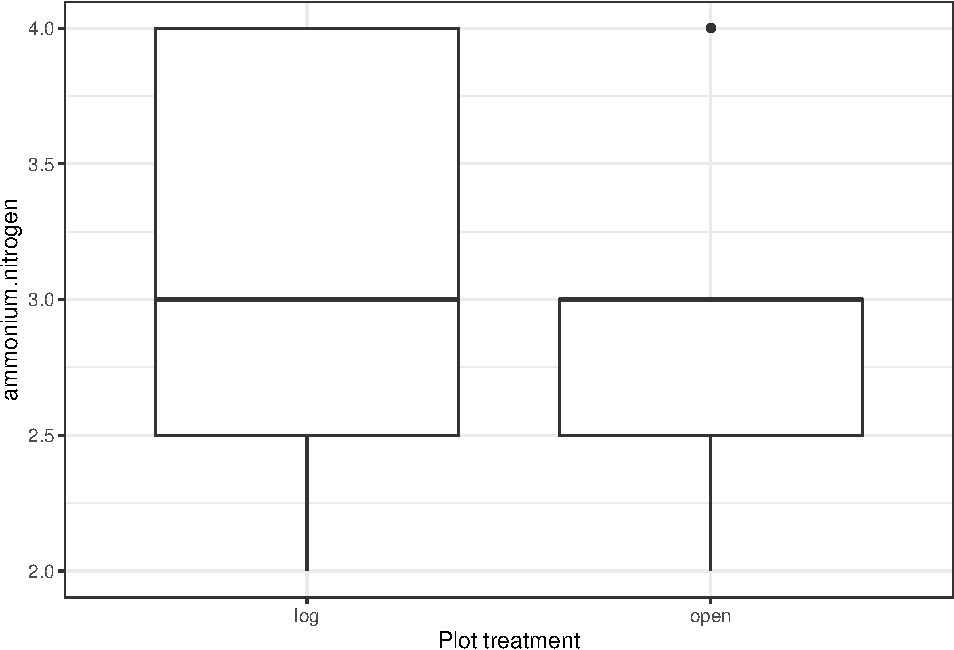
\includegraphics{log-project-aubrie-winnie_files/figure-latex/unnamed-chunk-8-1.pdf}
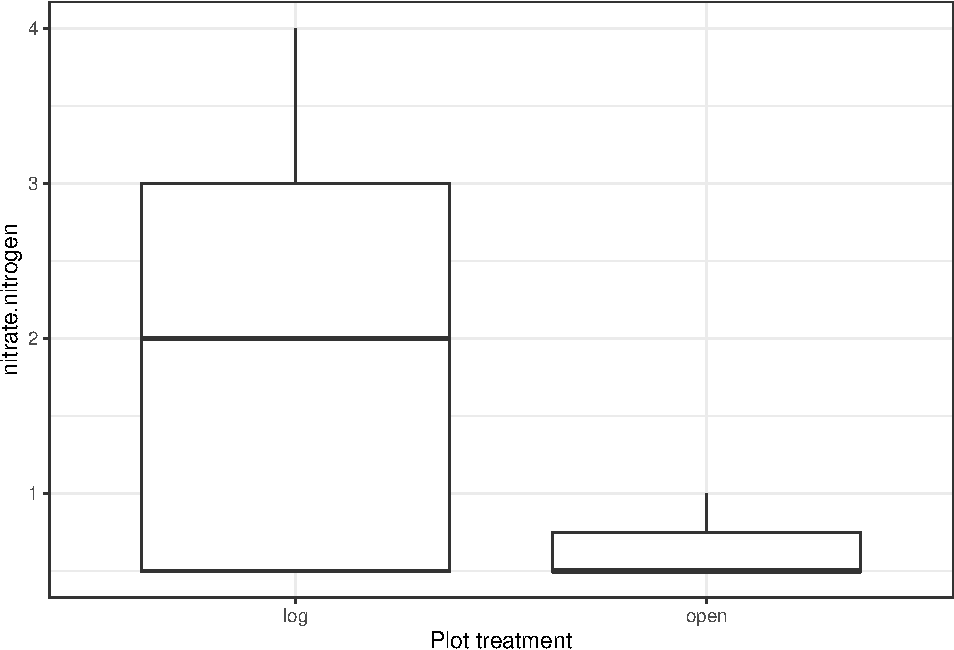
\includegraphics{log-project-aubrie-winnie_files/figure-latex/unnamed-chunk-8-2.pdf}
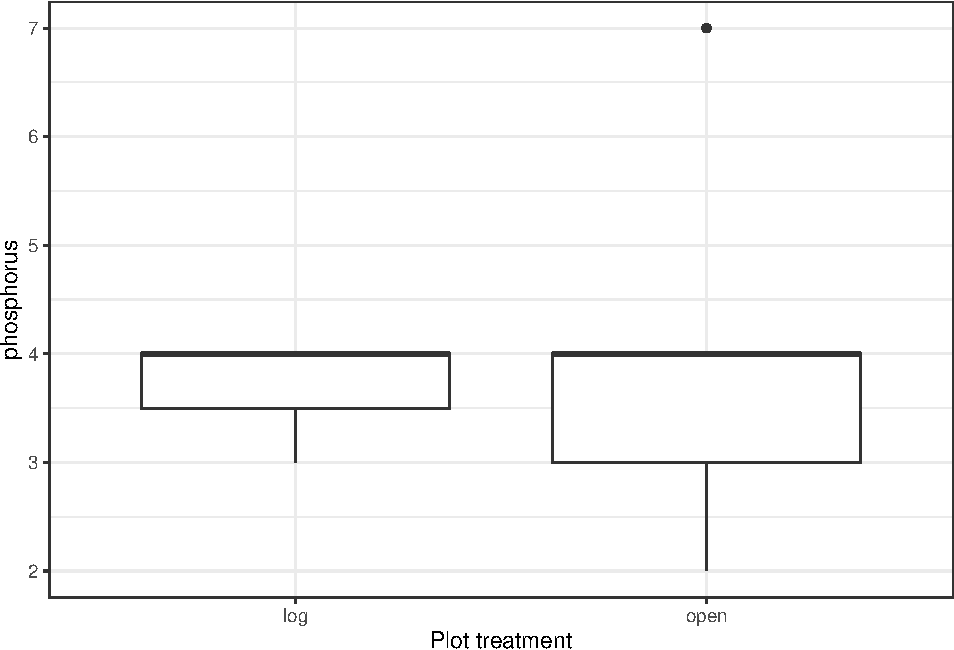
\includegraphics{log-project-aubrie-winnie_files/figure-latex/unnamed-chunk-8-3.pdf}
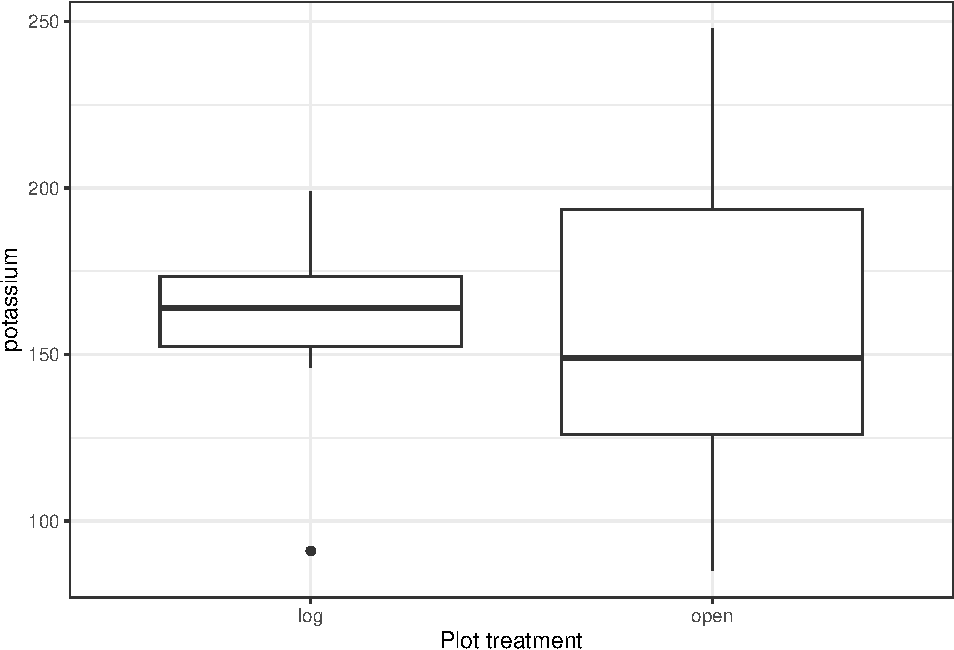
\includegraphics{log-project-aubrie-winnie_files/figure-latex/unnamed-chunk-8-4.pdf}
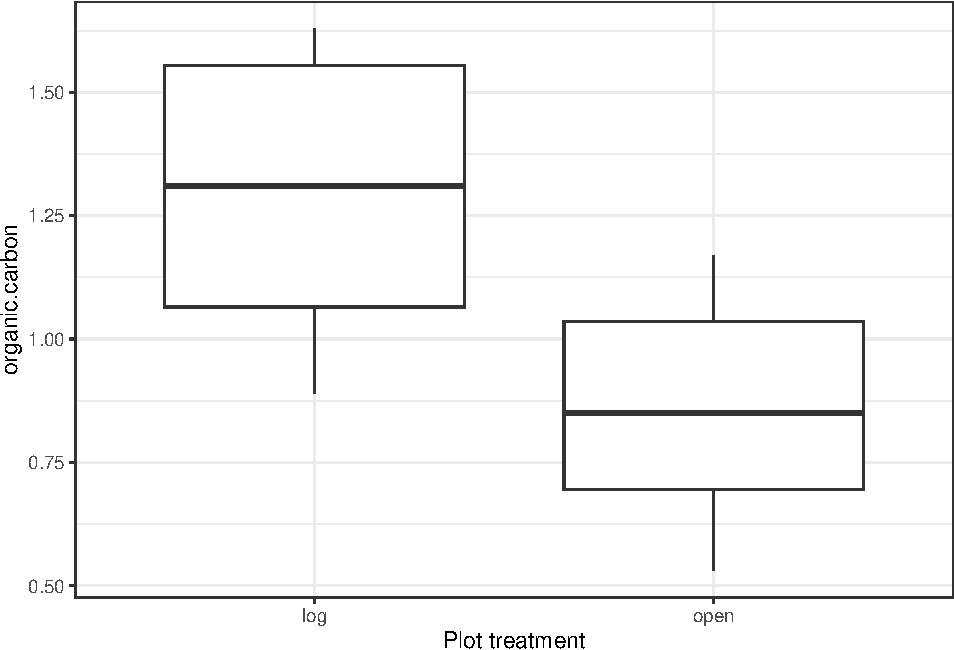
\includegraphics{log-project-aubrie-winnie_files/figure-latex/unnamed-chunk-8-5.pdf}
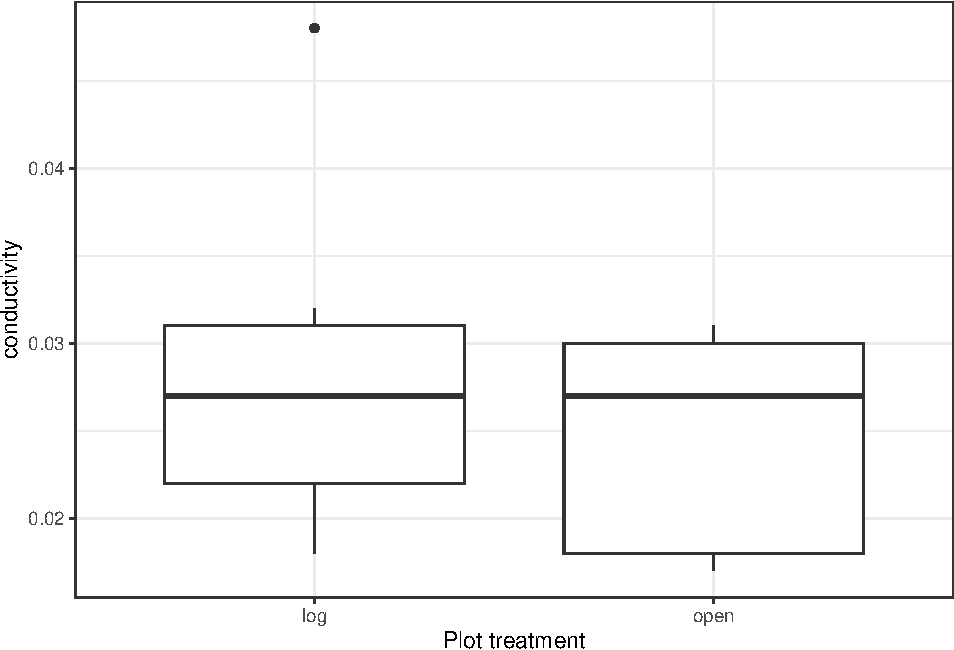
\includegraphics{log-project-aubrie-winnie_files/figure-latex/unnamed-chunk-8-6.pdf}
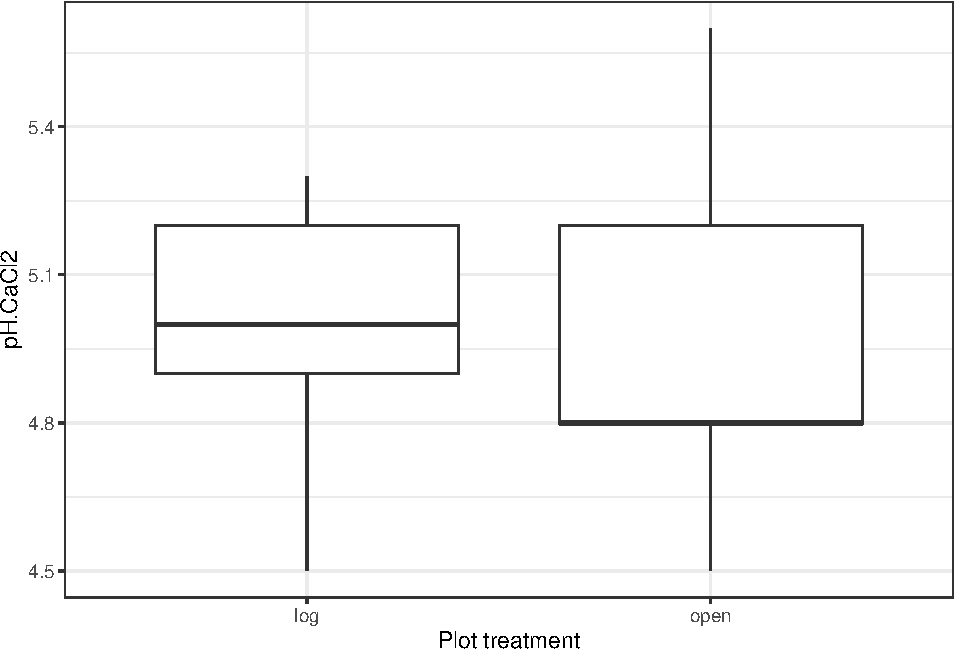
\includegraphics{log-project-aubrie-winnie_files/figure-latex/unnamed-chunk-8-7.pdf}
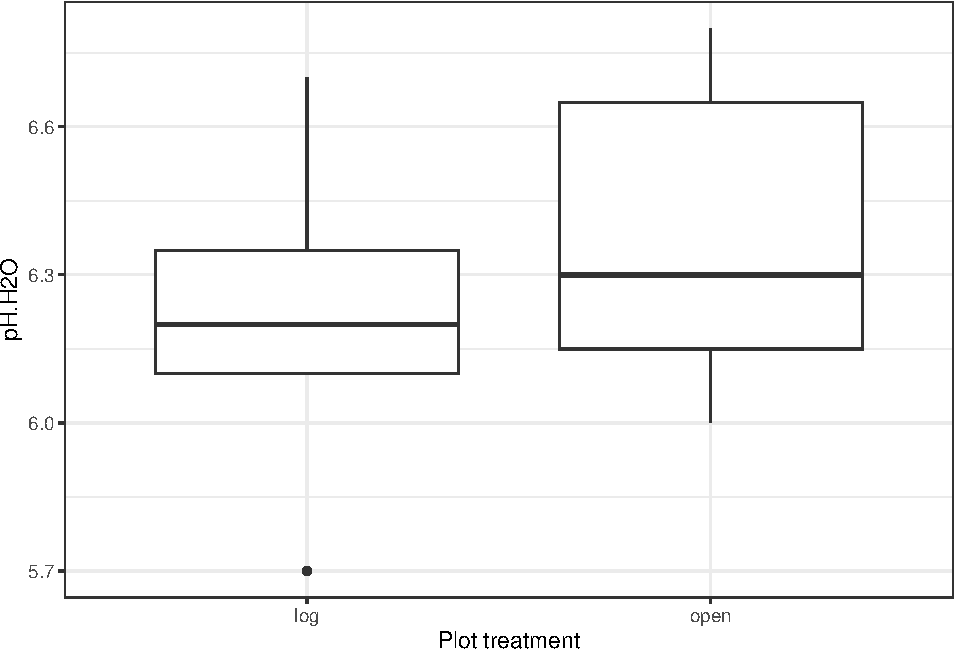
\includegraphics{log-project-aubrie-winnie_files/figure-latex/unnamed-chunk-8-8.pdf}
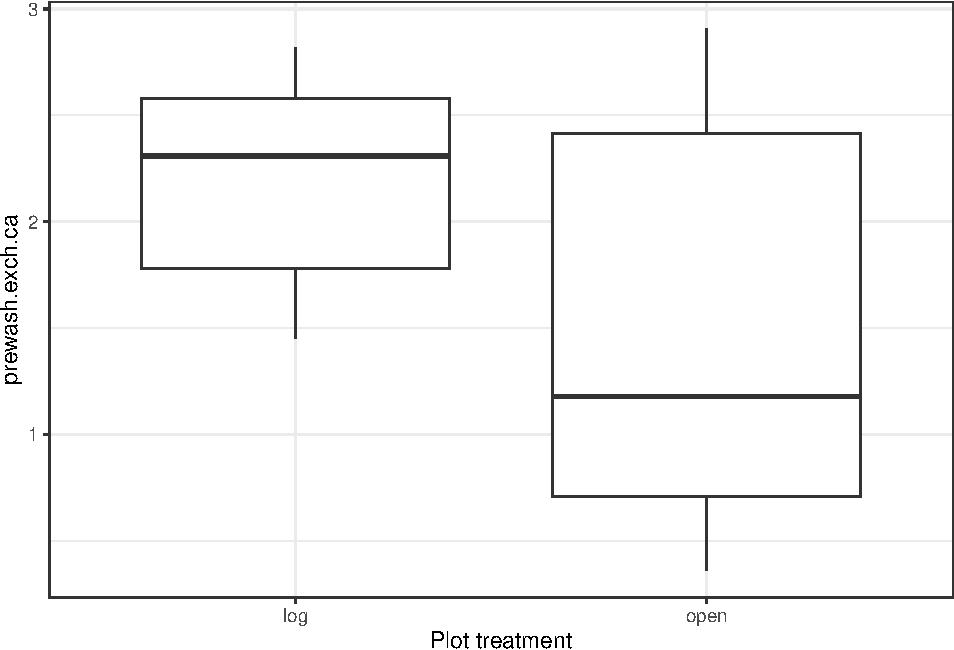
\includegraphics{log-project-aubrie-winnie_files/figure-latex/unnamed-chunk-8-9.pdf}
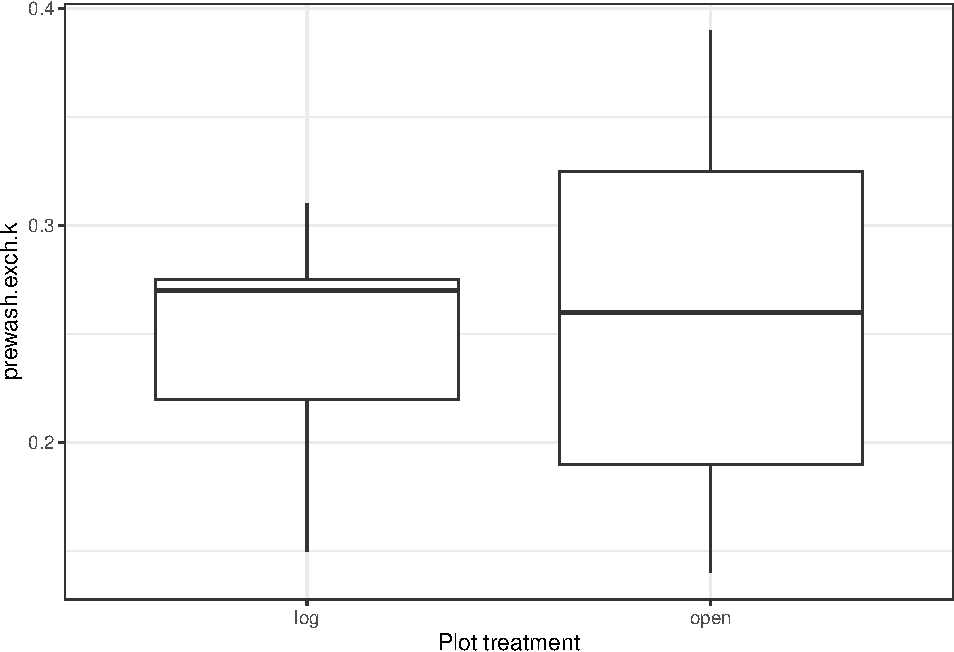
\includegraphics{log-project-aubrie-winnie_files/figure-latex/unnamed-chunk-8-10.pdf}
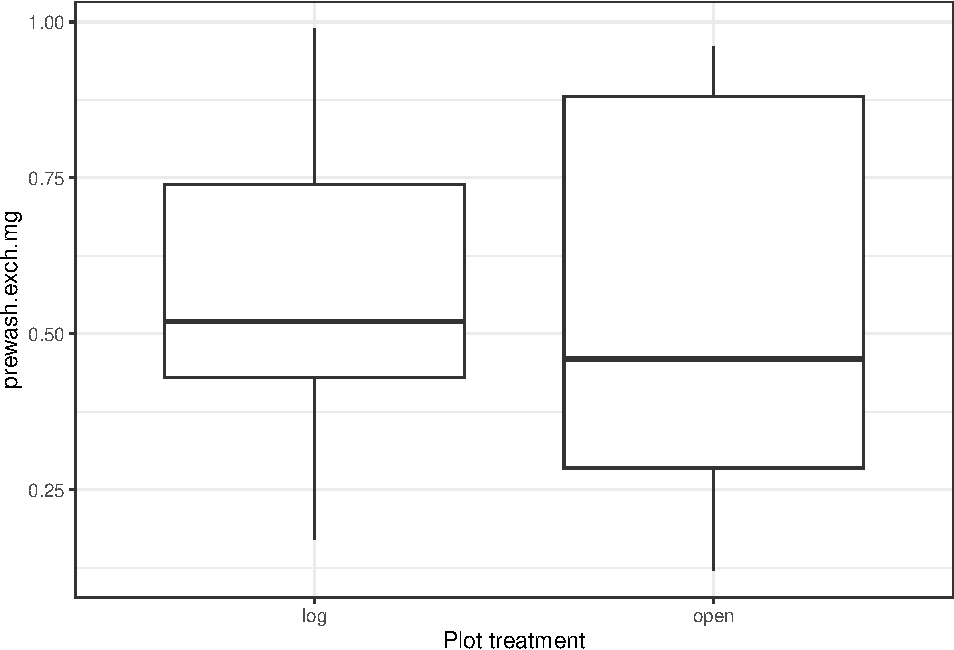
\includegraphics{log-project-aubrie-winnie_files/figure-latex/unnamed-chunk-8-11.pdf}

\begin{Shaded}
\begin{Highlighting}[]
\NormalTok{nutrient.for.pca }\OtherTok{\textless{}{-}}\NormalTok{ nutrient[,}\FunctionTok{c}\NormalTok{(}\DecValTok{7}\SpecialCharTok{:}\DecValTok{12}\NormalTok{,}\DecValTok{17}\NormalTok{)]}
\NormalTok{nutrient.pca }\OtherTok{\textless{}{-}} \FunctionTok{prcomp}\NormalTok{(nutrient.for.pca, }\AttributeTok{center=}\ConstantTok{TRUE}\NormalTok{, }\AttributeTok{scale=}\ConstantTok{TRUE}\NormalTok{)}
\FunctionTok{biplot}\NormalTok{(nutrient.pca)}
\end{Highlighting}
\end{Shaded}

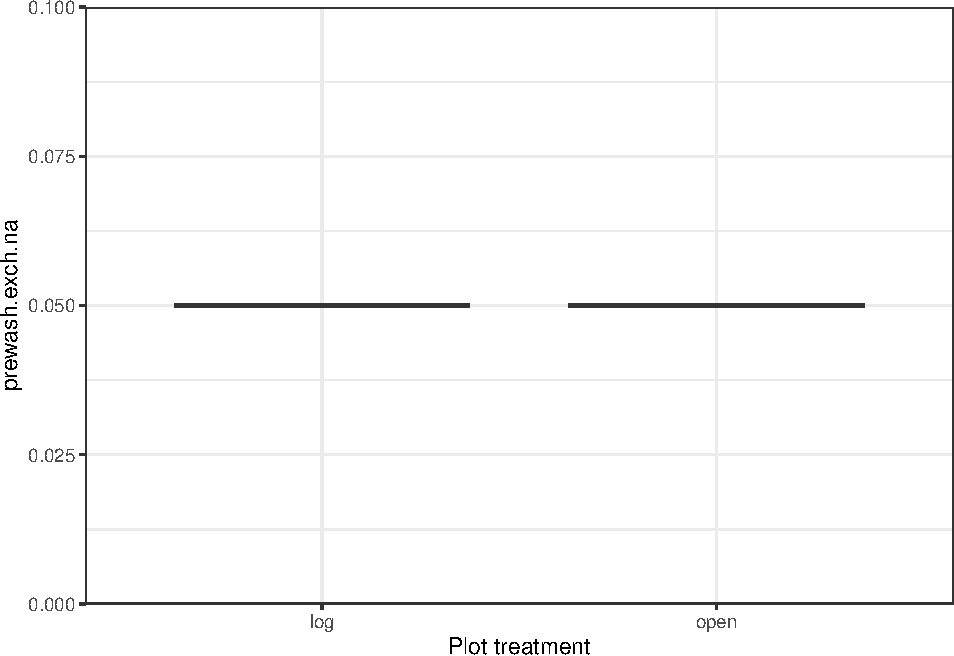
\includegraphics{log-project-aubrie-winnie_files/figure-latex/unnamed-chunk-8-12.pdf}

Nutrient composition comparison between log and open

\begin{itemize}
\tightlist
\item
  Organic carbon in soil is significantly higher in fallen log patches.
\end{itemize}

\begin{Shaded}
\begin{Highlighting}[]
\FunctionTok{library}\NormalTok{(ggplot2)}
\FunctionTok{library}\NormalTok{(ggpubr)}
\FunctionTok{library}\NormalTok{(dplyr)}
\FunctionTok{library}\NormalTok{(lme4)}
\FunctionTok{library}\NormalTok{(emmeans)}
\FunctionTok{library}\NormalTok{(pscl)}
\FunctionTok{library}\NormalTok{(glmmTMB)}
\FunctionTok{library}\NormalTok{(tidyr)}
\FunctionTok{library}\NormalTok{(DHARMa)}
\FunctionTok{library}\NormalTok{(ggplot2)}
\FunctionTok{library}\NormalTok{(AICcmodavg)}
\FunctionTok{library}\NormalTok{(ggpubr)}

\CommentTok{\# Set up nutrient analysis data}
\NormalTok{nutrient }\OtherTok{\textless{}{-}} \FunctionTok{read.csv}\NormalTok{(}\StringTok{"Nutrient.csv"}\NormalTok{, }\AttributeTok{header =}\NormalTok{ T)}
\NormalTok{nutrient }\OtherTok{\textless{}{-}}\FunctionTok{separate}\NormalTok{(nutrient,}\DecValTok{2}\NormalTok{ , }\FunctionTok{c}\NormalTok{(}\StringTok{"block"}\NormalTok{,}\StringTok{"plot"}\NormalTok{), }\StringTok{"\_"}\NormalTok{)}
\NormalTok{nutrient }\OtherTok{\textless{}{-}}\NormalTok{ nutrient[,}\DecValTok{2}\SpecialCharTok{:}\DecValTok{18}\NormalTok{]}

\NormalTok{Nu }\OtherTok{\textless{}{-}} \FunctionTok{c}\NormalTok{(}\StringTok{"N"}\NormalTok{, }\StringTok{"P"}\NormalTok{, }\StringTok{"K"}\NormalTok{, }\StringTok{"C"}\NormalTok{, }\StringTok{"pH"}\NormalTok{, }\StringTok{"CEC"}\NormalTok{, }\StringTok{"conductivity"}\NormalTok{)}

\NormalTok{wilcox\_results }\OtherTok{\textless{}{-}} \FunctionTok{data.frame}\NormalTok{(}\AttributeTok{element =} \FunctionTok{character}\NormalTok{(),}
                                \AttributeTok{w =} \FunctionTok{numeric}\NormalTok{(),}
                                \AttributeTok{p\_value =} \FunctionTok{numeric}\NormalTok{(),}
                                \AttributeTok{stringsAsFactors =} \ConstantTok{FALSE}\NormalTok{)}

\CommentTok{\# Perform Wilcoxon rank sum test for each element between treatments}
\NormalTok{nutrient}\SpecialCharTok{$}\NormalTok{init }\OtherTok{\textless{}{-}} \FunctionTok{as.factor}\NormalTok{(nutrient}\SpecialCharTok{$}\NormalTok{init)}
\ControlFlowTok{for}\NormalTok{ (element }\ControlFlowTok{in}\NormalTok{ Nu) \{}
\NormalTok{    result }\OtherTok{\textless{}{-}} \FunctionTok{wilcox.test}\NormalTok{(}\FunctionTok{get}\NormalTok{(element) }\SpecialCharTok{\textasciitilde{}}\NormalTok{ init, }\AttributeTok{data =}\NormalTok{ nutrient, }\AttributeTok{exact=}\ConstantTok{TRUE}\NormalTok{)}
\NormalTok{    wilcox\_results }\OtherTok{\textless{}{-}} \FunctionTok{rbind}\NormalTok{(wilcox\_results, }
                               \FunctionTok{data.frame}\NormalTok{(}\AttributeTok{element =}\NormalTok{ element,}
                                          \AttributeTok{w =}\NormalTok{ result}\SpecialCharTok{$}\NormalTok{statistic,}
                                          \AttributeTok{p\_value =}\NormalTok{ result}\SpecialCharTok{$}\NormalTok{p.value,}
                                          \AttributeTok{stringsAsFactors =} \ConstantTok{FALSE}\NormalTok{,}
                                          \AttributeTok{row.names =} \ConstantTok{NULL}\NormalTok{))}
\NormalTok{\}}

\FunctionTok{print}\NormalTok{(wilcox\_results) }\CommentTok{\# only organic carbon is significantly different between the two plot types}

\NormalTok{plots\_list }\OtherTok{\textless{}{-}} \FunctionTok{list}\NormalTok{()}

\ControlFlowTok{for}\NormalTok{ (element }\ControlFlowTok{in} \FunctionTok{c}\NormalTok{(Nu, }\StringTok{"C"}\NormalTok{)) \{}
  \ControlFlowTok{if}\NormalTok{ (element }\SpecialCharTok{==} \StringTok{"C"}\NormalTok{) \{}
\NormalTok{    plot }\OtherTok{\textless{}{-}} \FunctionTok{ggplot}\NormalTok{(nutrient, }\FunctionTok{aes}\NormalTok{(}\AttributeTok{x =}\NormalTok{ init, }\AttributeTok{y =}\NormalTok{ C)) }\SpecialCharTok{+}
      \FunctionTok{geom\_boxplot}\NormalTok{() }\SpecialCharTok{+} 
      \FunctionTok{theme\_bw}\NormalTok{() }\SpecialCharTok{+}
      \FunctionTok{labs}\NormalTok{(}\AttributeTok{x =} \ConstantTok{NULL}\NormalTok{, }\AttributeTok{y =} \StringTok{"C"}\NormalTok{) }\SpecialCharTok{+} 
      \FunctionTok{scale\_x\_discrete}\NormalTok{(}\AttributeTok{labels=}\FunctionTok{c}\NormalTok{(}\StringTok{\textquotesingle{}log\textquotesingle{}}\NormalTok{, }\StringTok{\textquotesingle{}open\textquotesingle{}}\NormalTok{)) }\SpecialCharTok{+}
      \FunctionTok{geom\_signif}\NormalTok{(}\AttributeTok{comparisons =} \FunctionTok{list}\NormalTok{(}\FunctionTok{c}\NormalTok{(}\StringTok{"log"}\NormalTok{, }\StringTok{"open"}\NormalTok{)),}
                  \AttributeTok{map\_signif\_level =} \ConstantTok{TRUE}\NormalTok{,}
                  \AttributeTok{textsize =} \DecValTok{5}\NormalTok{, }\AttributeTok{vjust =} \FloatTok{0.5}\NormalTok{, }\AttributeTok{y\_position =} \FloatTok{1.6}\NormalTok{, }\AttributeTok{tip\_length =} \DecValTok{0}\NormalTok{) }\SpecialCharTok{+} 
      \FunctionTok{scale\_y\_continuous}\NormalTok{(}\AttributeTok{expand =} \FunctionTok{c}\NormalTok{(}\DecValTok{0}\NormalTok{,}\FloatTok{0.1}\NormalTok{))}\SpecialCharTok{+}
      \FunctionTok{theme}\NormalTok{(}
    \AttributeTok{plot.background =} \FunctionTok{element\_blank}\NormalTok{(),}
    \AttributeTok{panel.grid.major =} \FunctionTok{element\_blank}\NormalTok{(),}
    \AttributeTok{panel.grid.minor =} \FunctionTok{element\_blank}\NormalTok{(),}
    \AttributeTok{panel.border =} \FunctionTok{element\_blank}\NormalTok{()) }\SpecialCharTok{+} 
      \FunctionTok{theme}\NormalTok{(}\AttributeTok{axis.line =} \FunctionTok{element\_line}\NormalTok{(}\AttributeTok{color =} \StringTok{\textquotesingle{}black\textquotesingle{}}\NormalTok{))}
    
\NormalTok{  \} }\ControlFlowTok{else}\NormalTok{ \{}
\NormalTok{    plot }\OtherTok{\textless{}{-}} \FunctionTok{ggplot}\NormalTok{(nutrient, }\FunctionTok{aes}\NormalTok{(}\AttributeTok{x =}\NormalTok{ init, }\AttributeTok{y =} \SpecialCharTok{!!}\NormalTok{rlang}\SpecialCharTok{::}\FunctionTok{sym}\NormalTok{(element))) }\SpecialCharTok{+}
      \FunctionTok{geom\_boxplot}\NormalTok{() }\SpecialCharTok{+} 
      \FunctionTok{theme\_bw}\NormalTok{() }\SpecialCharTok{+}
      \FunctionTok{labs}\NormalTok{(}\AttributeTok{x =} \ConstantTok{NULL}\NormalTok{, }\AttributeTok{y =}\NormalTok{ element) }\SpecialCharTok{+} 
      \FunctionTok{scale\_x\_discrete}\NormalTok{(}\AttributeTok{labels=}\FunctionTok{c}\NormalTok{(}\StringTok{\textquotesingle{}log\textquotesingle{}}\NormalTok{, }\StringTok{\textquotesingle{}open\textquotesingle{}}\NormalTok{)) }\SpecialCharTok{+}
      \FunctionTok{theme}\NormalTok{(}
    \AttributeTok{plot.background =} \FunctionTok{element\_blank}\NormalTok{(),}
    \AttributeTok{panel.grid.major =} \FunctionTok{element\_blank}\NormalTok{(),}
    \AttributeTok{panel.grid.minor =} \FunctionTok{element\_blank}\NormalTok{(),}
    \AttributeTok{panel.border =} \FunctionTok{element\_blank}\NormalTok{()) }\SpecialCharTok{+} \FunctionTok{theme}\NormalTok{(}\AttributeTok{axis.line =} \FunctionTok{element\_line}\NormalTok{(}\AttributeTok{color =} \StringTok{\textquotesingle{}black\textquotesingle{}}\NormalTok{))}
\NormalTok{  \}}
  
\NormalTok{  plots\_list[[element]] }\OtherTok{\textless{}{-}}\NormalTok{ plot}
\NormalTok{\}}

\NormalTok{all.bp }\OtherTok{\textless{}{-}} \FunctionTok{ggarrange}\NormalTok{(}\AttributeTok{plotlist=}\NormalTok{plots\_list, }\AttributeTok{ncol=}\DecValTok{3}\NormalTok{, }\AttributeTok{nrow=}\DecValTok{3}\NormalTok{, }\AttributeTok{common.legend =}\ConstantTok{TRUE}\NormalTok{, }\AttributeTok{legend=}\StringTok{"bottom"}\NormalTok{,}\AttributeTok{align =} \StringTok{"v"}\NormalTok{)}

\NormalTok{all.bp }\OtherTok{\textless{}{-}} \FunctionTok{annotate\_figure}\NormalTok{(all.bp, }\AttributeTok{bottom =} \StringTok{"Plot treatment"}\NormalTok{)}
\CommentTok{\# Show the final plot}
\FunctionTok{print}\NormalTok{(all.bp)}
\end{Highlighting}
\end{Shaded}

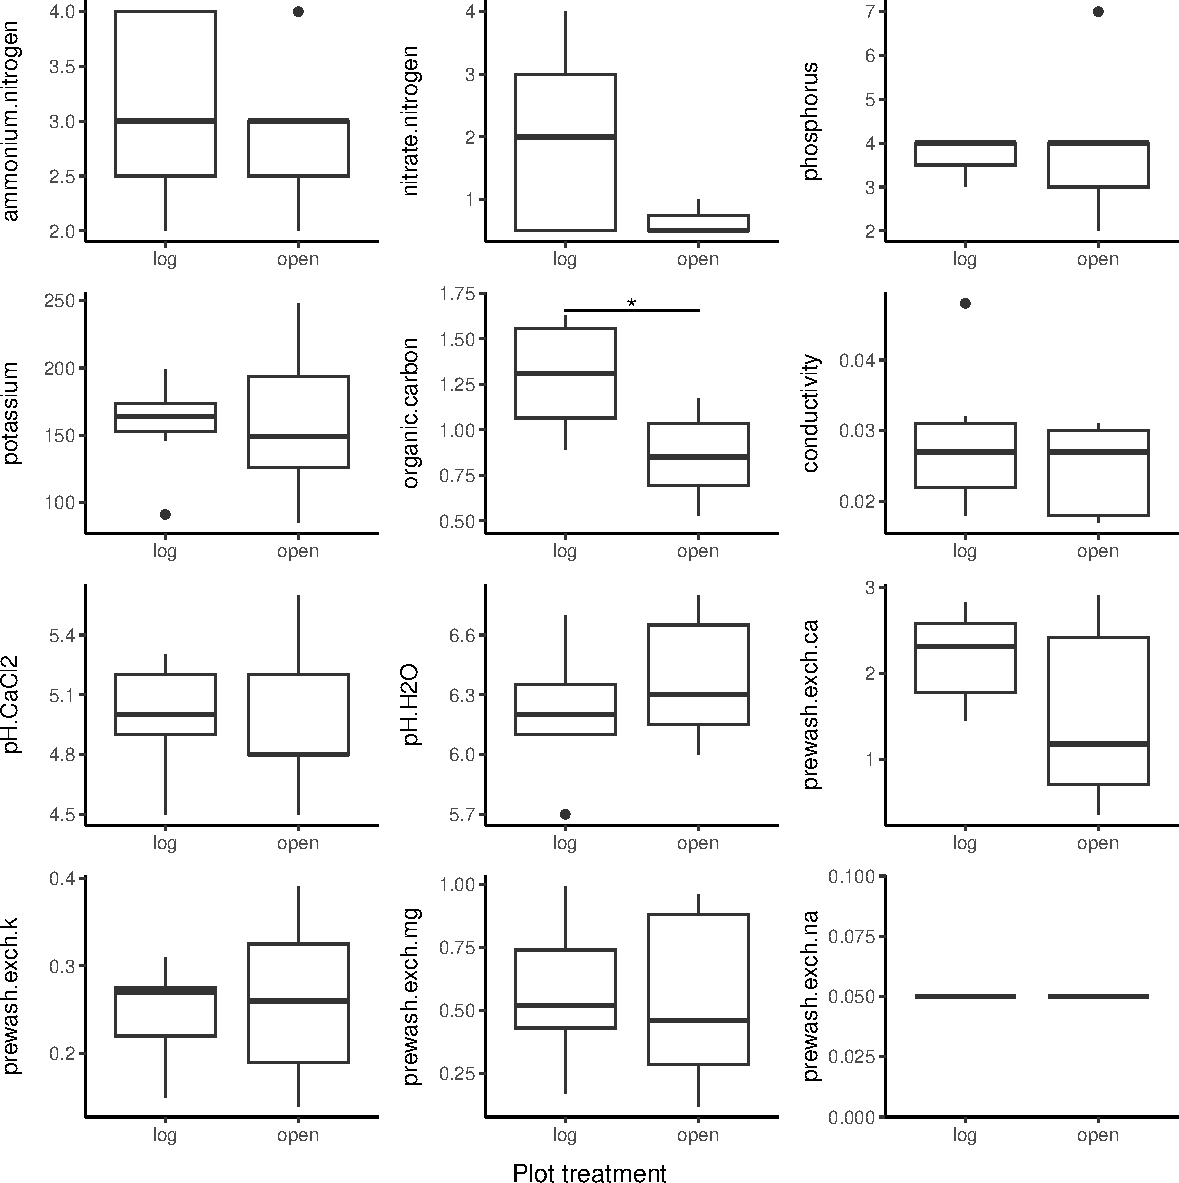
\includegraphics{log-project-aubrie-winnie_files/figure-latex/unnamed-chunk-9-1.pdf}

\begin{verbatim}
##        element    w    p_value
## 1            N 41.5 0.03126054
## 2            P 26.5 0.82963146
## 3            K 26.0 0.90151515
## 4            C 42.5 0.02518656
## 5           pH 29.5 0.56096176
## 6          CEC 30.0 0.53496503
## 7 conductivity 30.5 0.47929050
\end{verbatim}

\hypertarget{abundance-nutrient-composition}{%
\subparagraph{Abundance \textasciitilde{} nutrient
composition}\label{abundance-nutrient-composition}}

\begin{Shaded}
\begin{Highlighting}[]
\FunctionTok{library}\NormalTok{(ggplot2)}
\FunctionTok{library}\NormalTok{(ggpubr)}
\FunctionTok{library}\NormalTok{(dplyr)}
\FunctionTok{library}\NormalTok{(lme4)}
\FunctionTok{library}\NormalTok{(emmeans)}
\FunctionTok{library}\NormalTok{(pscl)}
\FunctionTok{library}\NormalTok{(glmmTMB)}
\FunctionTok{library}\NormalTok{(tidyr)}
\FunctionTok{library}\NormalTok{(DHARMa)}
\FunctionTok{library}\NormalTok{(ggplot2)}
\FunctionTok{library}\NormalTok{(AICcmodavg)}
\FunctionTok{library}\NormalTok{(ggpubr)}
\FunctionTok{require}\NormalTok{(vegan)}
\FunctionTok{require}\NormalTok{(labdsv)}
\FunctionTok{require}\NormalTok{(stringr)}
\FunctionTok{require}\NormalTok{(ggrepel)}
\FunctionTok{library}\NormalTok{(car)}
\FunctionTok{library}\NormalTok{(sjPlot)}
\FunctionTok{library}\NormalTok{(sjmisc)}
\FunctionTok{library}\NormalTok{(sjlabelled)}
\FunctionTok{library}\NormalTok{(MuMIn)}

\CommentTok{\# Set up nutrient analysis data}
\NormalTok{nutrient }\OtherTok{\textless{}{-}} \FunctionTok{read.csv}\NormalTok{(}\StringTok{"Nutrient.csv"}\NormalTok{, }\AttributeTok{header =}\NormalTok{ T)}
\NormalTok{nutrient }\OtherTok{\textless{}{-}}\FunctionTok{separate}\NormalTok{(nutrient,}\DecValTok{2}\NormalTok{ , }\FunctionTok{c}\NormalTok{(}\StringTok{"block"}\NormalTok{,}\StringTok{"plot"}\NormalTok{), }\StringTok{"\_"}\NormalTok{)}
\NormalTok{nutrient }\OtherTok{\textless{}{-}}\NormalTok{ nutrient[,}\DecValTok{2}\SpecialCharTok{:}\DecValTok{18}\NormalTok{]}

\CommentTok{\# This community data set includes all species (including unidentified species)}
\NormalTok{comm }\OtherTok{\textless{}{-}} \FunctionTok{read.csv}\NormalTok{(}\StringTok{"20{-}22\_species\_composition\_data\_w\_unk.csv"}\NormalTok{, }\AttributeTok{header=}\NormalTok{T)}

\CommentTok{\# Remove the locations surveyed in 2021 and 2022 that were not surveyed in 2020 {-} aka, cm=0, cm=21, cm = 22, cm = 29.}
\NormalTok{comm}\OtherTok{\textless{}{-}}\NormalTok{comm[}\FunctionTok{which}\NormalTok{(comm}\SpecialCharTok{$}\NormalTok{cm\_location}\SpecialCharTok{!=}\DecValTok{21} \SpecialCharTok{\&}\NormalTok{ comm}\SpecialCharTok{$}\NormalTok{cm\_location}\SpecialCharTok{!=}\DecValTok{0} \SpecialCharTok{\&}\NormalTok{ comm}\SpecialCharTok{$}\NormalTok{cm\_location}\SpecialCharTok{!=}\DecValTok{22} \SpecialCharTok{\&}\NormalTok{ comm}\SpecialCharTok{$}\NormalTok{cm\_location}\SpecialCharTok{!=}\DecValTok{29}\NormalTok{),]}

\CommentTok{\# make a group name for each row}
\NormalTok{comm}\SpecialCharTok{$}\NormalTok{grp}\OtherTok{\textless{}{-}}\FunctionTok{apply}\NormalTok{(comm[}\FunctionTok{c}\NormalTok{(}\DecValTok{1}\NormalTok{,}\DecValTok{3}\NormalTok{,}\DecValTok{5}\NormalTok{,}\DecValTok{6}\NormalTok{,}\DecValTok{7}\NormalTok{)], }\DecValTok{1}\NormalTok{, paste, }\AttributeTok{collapse=}\StringTok{":"}\NormalTok{) }\CommentTok{\# timepoint, block, transect\_name, initial state}

\CommentTok{\# Need to make each row a community using matrify.}
\NormalTok{commsub}\OtherTok{\textless{}{-}}\NormalTok{comm[,}\FunctionTok{c}\NormalTok{(}\DecValTok{15}\NormalTok{,}\DecValTok{10}\NormalTok{,}\DecValTok{13}\NormalTok{)] }\CommentTok{\# group, species\_code, and count of each species for each transect. transects are rows.}
\NormalTok{commsub }\OtherTok{\textless{}{-}}\FunctionTok{as.data.frame}\NormalTok{(commsub)}
\NormalTok{commtry}\OtherTok{\textless{}{-}}\FunctionTok{matrify}\NormalTok{(commsub) }\CommentTok{\# make it an expanded species matrix }
\NormalTok{commtry}\SpecialCharTok{$}\NormalTok{x[}\FunctionTok{which}\NormalTok{(}\FunctionTok{is.na}\NormalTok{(commtry}\SpecialCharTok{$}\NormalTok{x))] }\OtherTok{\textless{}{-}} \DecValTok{1} \CommentTok{\# "x" means that there were no individuals in the transect, but we are going to keep track of this as if it were a species}
\CommentTok{\# ncol(commtry) \# how many species are we working with in our community matrix}

\CommentTok{\# Store grouping row names as a column, then remove rownames.}
\NormalTok{commtry}\SpecialCharTok{$}\NormalTok{grps}\OtherTok{\textless{}{-}}\FunctionTok{rownames}\NormalTok{(commtry)}
\FunctionTok{rownames}\NormalTok{(commtry)}\OtherTok{\textless{}{-}}\ConstantTok{NULL}
\CommentTok{\# names(commtry)}

\CommentTok{\# Split group info into columns for each variable.}
\NormalTok{mat}\OtherTok{\textless{}{-}}\FunctionTok{separate}\NormalTok{(commtry, }\DecValTok{107}\NormalTok{, }\FunctionTok{c}\NormalTok{(}\StringTok{"time"}\NormalTok{,}\StringTok{"block"}\NormalTok{,}\StringTok{"transect"}\NormalTok{,}\StringTok{"init"}\NormalTok{, }\StringTok{"treatment"}\NormalTok{), }\StringTok{":"}\NormalTok{)}
\CommentTok{\# names(mat) \#check}

\CommentTok{\# Add groupname using time, block, init columns.}
\NormalTok{mat}\SpecialCharTok{$}\NormalTok{grp1}\OtherTok{\textless{}{-}}\FunctionTok{apply}\NormalTok{(mat[}\FunctionTok{c}\NormalTok{(}\DecValTok{107}\SpecialCharTok{:}\DecValTok{110}\NormalTok{)], }\DecValTok{1}\NormalTok{, paste, }\AttributeTok{collapse=}\StringTok{":"}\NormalTok{)}
\NormalTok{mat}\SpecialCharTok{$}\NormalTok{grp2}\OtherTok{\textless{}{-}}\FunctionTok{apply}\NormalTok{(mat[}\FunctionTok{c}\NormalTok{(}\DecValTok{107}\SpecialCharTok{:}\DecValTok{111}\NormalTok{)], }\DecValTok{1}\NormalTok{, paste, }\AttributeTok{collapse=}\StringTok{":"}\NormalTok{)}
\CommentTok{\# names(mat) \#check}

\CommentTok{\# Another df where the grouping variables are time, block, transect and initial state.}
\CommentTok{\# Each row is a transect in a certain year.}
\NormalTok{df}\OtherTok{\textless{}{-}}\NormalTok{mat[,}\FunctionTok{c}\NormalTok{(}\DecValTok{1}\SpecialCharTok{:}\DecValTok{106}\NormalTok{,}\DecValTok{113}\NormalTok{)]}
\CommentTok{\# df2 = with treatment in the grouping}
\NormalTok{df2 }\OtherTok{=}\NormalTok{ df }\SpecialCharTok{\%\textgreater{}\%} \FunctionTok{mutate}\NormalTok{(}\FunctionTok{across}\NormalTok{(}\AttributeTok{.cols=}\DecValTok{1}\SpecialCharTok{:}\DecValTok{106}\NormalTok{,}\AttributeTok{.fns=}\NormalTok{as.numeric))}
\FunctionTok{rownames}\NormalTok{(df2)}\OtherTok{\textless{}{-}}\ConstantTok{NULL} \CommentTok{\# remove rownames}

\DocumentationTok{\#\#\#\#\# Abundance analysis for 2020 (t0) AND in{-}situ log and in{-}situ open plots in 2021 (t1) and 2022 (t2)}

\CommentTok{\# Sum observations across initial X transect X time X  block X treatment (group variable).}
\CommentTok{\# This gives number of plants in each row observation (transect level).}
\NormalTok{blocksum2}\OtherTok{\textless{}{-}}\FunctionTok{rowsum}\NormalTok{(df2[,}\FunctionTok{c}\NormalTok{(}\DecValTok{1}\SpecialCharTok{:}\DecValTok{106}\NormalTok{)], }\AttributeTok{group=}\NormalTok{df2}\SpecialCharTok{$}\NormalTok{grp2)}
\NormalTok{blocksum2}\SpecialCharTok{$}\NormalTok{grps}\OtherTok{\textless{}{-}}\FunctionTok{rownames}\NormalTok{(blocksum2)}
\FunctionTok{rownames}\NormalTok{(blocksum2)}\OtherTok{\textless{}{-}}\ConstantTok{NULL} \CommentTok{\# remove rownames}

\CommentTok{\# Add in group vars.}
\NormalTok{nublock2}\OtherTok{\textless{}{-}}\FunctionTok{separate}\NormalTok{(blocksum2, }\DecValTok{107}\NormalTok{, }\FunctionTok{c}\NormalTok{(}\StringTok{"time"}\NormalTok{,}\StringTok{"block"}\NormalTok{,}\StringTok{"transect"}\NormalTok{,}\StringTok{"init"}\NormalTok{, }\StringTok{"treatment"}\NormalTok{), }\StringTok{":"}\NormalTok{)}
\NormalTok{nublock2}\SpecialCharTok{$}\NormalTok{total}\OtherTok{\textless{}{-}}\FunctionTok{rowSums}\NormalTok{(nublock2[,}\FunctionTok{c}\NormalTok{(}\DecValTok{1}\SpecialCharTok{:}\DecValTok{106}\NormalTok{)])}
\NormalTok{nublock2}\SpecialCharTok{$}\NormalTok{presence}\OtherTok{\textless{}{-}}\FunctionTok{ifelse}\NormalTok{(nublock2}\SpecialCharTok{$}\NormalTok{total }\SpecialCharTok{\textgreater{}} \DecValTok{0}\NormalTok{,  }\DecValTok{1}\NormalTok{, }\DecValTok{0}\NormalTok{)}

\CommentTok{\# Subset data where before treatments installed (t0), in{-}situ log and in{-}situ open from t1 and t2 are included.}
\CommentTok{\# Hence only absolute log effect and absolute open effect are concerned}
\NormalTok{dat\_t0\_insitu}\OtherTok{\textless{}{-}}\NormalTok{nublock2[}\FunctionTok{which}\NormalTok{(nublock2}\SpecialCharTok{$}\NormalTok{time}\SpecialCharTok{==}\StringTok{"t0"} \SpecialCharTok{|}\NormalTok{  nublock2}\SpecialCharTok{$}\NormalTok{treatment}\SpecialCharTok{==}\StringTok{"open"} \SpecialCharTok{|}\NormalTok{  nublock2}\SpecialCharTok{$}\NormalTok{treatment}\SpecialCharTok{==}\StringTok{"insitu\_log"}\NormalTok{),]}

\CommentTok{\# look at plant abundance in log vs open }
\CommentTok{\# look at range of data {-} what family should i use? }
\CommentTok{\# range(dat\_t0\_insitu$total)}
\NormalTok{nutrient\_join }\OtherTok{\textless{}{-}}\NormalTok{ nutrient[,}\FunctionTok{c}\NormalTok{(}\DecValTok{1}\NormalTok{,}\DecValTok{3}\NormalTok{, }\DecValTok{7}\SpecialCharTok{:}\DecValTok{12}\NormalTok{,}\DecValTok{17}\NormalTok{)]}
\NormalTok{nutrient\_join[,}\DecValTok{3}\SpecialCharTok{:}\DecValTok{9}\NormalTok{] }\OtherTok{\textless{}{-}} \FunctionTok{scale}\NormalTok{(nutrient\_join[,}\DecValTok{3}\SpecialCharTok{:}\DecValTok{9}\NormalTok{])}
\NormalTok{dat\_t0\_insitu }\OtherTok{\textless{}{-}} \FunctionTok{inner\_join}\NormalTok{(dat\_t0\_insitu, nutrient\_join, }\AttributeTok{by =} \FunctionTok{c}\NormalTok{(}\StringTok{"init"}\NormalTok{, }\StringTok{"block"}\NormalTok{))}

\CommentTok{\# since samples from t1 and t2 from are mainly from the same plots as t0. These are not independent replicates and tend to correlated with each other.}
\CommentTok{\# including year and block as random effects}
\CommentTok{\# (1|year) + (1|block) as we think the effect of init on total is the same (slope) but the intercept differ amongst block and year}
\CommentTok{\# but since we have a greater number of sample from t0, data from t0 will contribute more to the variance in abundance.}
\CommentTok{\# see https://bookdown.org/steve\_midway/DAR/random{-}effects.html\#pld{-}example}

\CommentTok{\# 2020 {-} 2022 \#}
\NormalTok{mod.dredge }\OtherTok{\textless{}{-}} \FunctionTok{glm}\NormalTok{(total}\SpecialCharTok{\textasciitilde{}}\NormalTok{ N}\SpecialCharTok{+}\NormalTok{ P }\SpecialCharTok{+}\NormalTok{ K }\SpecialCharTok{+}\NormalTok{ C }\SpecialCharTok{+}\NormalTok{ CEC, }\AttributeTok{data =}\NormalTok{ dat\_t0\_insitu, }\AttributeTok{family =}\NormalTok{ poisson,}\AttributeTok{na.action =} \StringTok{"na.fail"}\NormalTok{)}
\CommentTok{\# vif(mod.dredge) \# no collinearity}
\NormalTok{dredge\_allyear }\OtherTok{\textless{}{-}} \FunctionTok{dredge}\NormalTok{(mod.dredge, }\AttributeTok{extra =} \StringTok{"adjR\^{}2"}\NormalTok{) }\CommentTok{\# candidate model including all nutrient elements are fairly good compared to the best fitting model}
\NormalTok{best.allyear }\OtherTok{\textless{}{-}} \FunctionTok{glm}\NormalTok{(total}\SpecialCharTok{\textasciitilde{}}\NormalTok{ N}\SpecialCharTok{+}\NormalTok{ C }\SpecialCharTok{+}\NormalTok{ CEC, }\AttributeTok{data =}\NormalTok{ dat\_t0\_insitu, }\AttributeTok{family =}\NormalTok{ poisson)}
\NormalTok{selected.allyear }\OtherTok{\textless{}{-}} \FunctionTok{glm}\NormalTok{(total}\SpecialCharTok{\textasciitilde{}}\NormalTok{ N}\SpecialCharTok{+}\NormalTok{ P }\SpecialCharTok{+}\NormalTok{ K }\SpecialCharTok{+}\NormalTok{ C }\SpecialCharTok{+}\NormalTok{ CEC, }\AttributeTok{data =}\NormalTok{ dat\_t0\_insitu, }\AttributeTok{family =}\NormalTok{ poisson)}
\FunctionTok{tab\_model}\NormalTok{(best.allyear,selected.allyear,mod.dredge, }\AttributeTok{file=}\StringTok{"mod.abun\_nu\_allyear.html"}\NormalTok{,  }\AttributeTok{dv.labels =} \FunctionTok{c}\NormalTok{(}\StringTok{"Best model"}\NormalTok{, }\StringTok{"Selected model"}\NormalTok{, }\StringTok{"Inclusive model (all years)"}\NormalTok{))}
\NormalTok{htmltools}\SpecialCharTok{::}\FunctionTok{includeHTML}\NormalTok{(}\StringTok{"mod.abun\_nu\_allyear.html"}\NormalTok{)}

\CommentTok{\# only 2022 \#}
\NormalTok{mod.dredge}\FloatTok{.2022} \OtherTok{\textless{}{-}} \FunctionTok{glm}\NormalTok{(total}\SpecialCharTok{\textasciitilde{}}\NormalTok{ N}\SpecialCharTok{+}\NormalTok{ P }\SpecialCharTok{+}\NormalTok{ K }\SpecialCharTok{+}\NormalTok{ C }\SpecialCharTok{+}\NormalTok{ CEC, }\AttributeTok{data =}\NormalTok{ dat\_t0\_insitu,}\AttributeTok{subset =}\NormalTok{ (time }\SpecialCharTok{==} \StringTok{"t2"}\NormalTok{), }\AttributeTok{family =}\NormalTok{ poisson, }\AttributeTok{na.action =} \StringTok{"na.fail"}\NormalTok{)}
\CommentTok{\# vif(mod.dredge.2022) \# no collinearity}
\NormalTok{dredge\_2022 }\OtherTok{\textless{}{-}} \FunctionTok{dredge}\NormalTok{(mod.dredge}\FloatTok{.2022}\NormalTok{, }\AttributeTok{extra =} \StringTok{"adjR\^{}2"}\NormalTok{) }\CommentTok{\# candidate model including all nutrient elements are fairly good compared to the best fitting model}
\NormalTok{best}\FloatTok{.2022} \OtherTok{\textless{}{-}} \FunctionTok{glm}\NormalTok{(total}\SpecialCharTok{\textasciitilde{}}\NormalTok{ N}\SpecialCharTok{+}\NormalTok{ P }\SpecialCharTok{+}\NormalTok{ C }\SpecialCharTok{+}\NormalTok{ CEC }\SpecialCharTok{+}\NormalTok{ conductivity, }\AttributeTok{data =}\NormalTok{ dat\_t0\_insitu,}\AttributeTok{subset =}\NormalTok{ (time }\SpecialCharTok{==} \StringTok{"t2"}\NormalTok{), }\AttributeTok{family =}\NormalTok{ poisson)}
\FunctionTok{tab\_model}\NormalTok{(best}\FloatTok{.2022}\NormalTok{,mod.dredge}\FloatTok{.2022}\NormalTok{, }\AttributeTok{file=}\StringTok{"mod.abun\_nu\_2022.html"}\NormalTok{, }\AttributeTok{dv.labels =} \FunctionTok{c}\NormalTok{(}\StringTok{"Best model"}\NormalTok{, }\StringTok{"Selected inclusive model (2022)"}\NormalTok{))}
\NormalTok{htmltools}\SpecialCharTok{::}\FunctionTok{includeHTML}\NormalTok{(}\StringTok{"mod.abun\_nu\_2022.html"}\NormalTok{)}

\CommentTok{\# only 2021 \#}
\NormalTok{mod.dredge}\FloatTok{.2021} \OtherTok{\textless{}{-}} \FunctionTok{glm}\NormalTok{(total}\SpecialCharTok{\textasciitilde{}}\NormalTok{ N}\SpecialCharTok{+}\NormalTok{ P }\SpecialCharTok{+}\NormalTok{ K }\SpecialCharTok{+}\NormalTok{ C }\SpecialCharTok{+}\NormalTok{ CEC, }\AttributeTok{data =}\NormalTok{ dat\_t0\_insitu, }\AttributeTok{subset =}\NormalTok{ (time }\SpecialCharTok{==} \StringTok{"t1"}\NormalTok{), }\AttributeTok{family =}\NormalTok{ poisson ,}\AttributeTok{na.action =} \StringTok{"na.fail"}\NormalTok{)}
\CommentTok{\# vif(mod.dredge.2021) \# no collinearity}
\NormalTok{dredge\_2021 }\OtherTok{\textless{}{-}} \FunctionTok{dredge}\NormalTok{(mod.dredge}\FloatTok{.2021}\NormalTok{, }\AttributeTok{extra =} \StringTok{"adjR\^{}2"}\NormalTok{)}
\NormalTok{best}\FloatTok{.2021} \OtherTok{\textless{}{-}} \FunctionTok{glm}\NormalTok{(total}\SpecialCharTok{\textasciitilde{}}\NormalTok{ K }\SpecialCharTok{+}\NormalTok{ N }\SpecialCharTok{+}\NormalTok{ P, }\AttributeTok{data =}\NormalTok{ dat\_t0\_insitu, }\AttributeTok{subset =}\NormalTok{ (time }\SpecialCharTok{==} \StringTok{"t1"}\NormalTok{), }\AttributeTok{family =}\NormalTok{ poisson)}
\NormalTok{selected}\FloatTok{.2021} \OtherTok{\textless{}{-}} \FunctionTok{glm}\NormalTok{(total}\SpecialCharTok{\textasciitilde{}}\NormalTok{ N}\SpecialCharTok{+}\NormalTok{ P }\SpecialCharTok{+}\NormalTok{ K }\SpecialCharTok{+}\NormalTok{ C, }\AttributeTok{data =}\NormalTok{ dat\_t0\_insitu, }\AttributeTok{subset =}\NormalTok{ (time }\SpecialCharTok{==} \StringTok{"t1"}\NormalTok{), }\AttributeTok{family =}\NormalTok{ poisson)}
\FunctionTok{tab\_model}\NormalTok{(best}\FloatTok{.2021}\NormalTok{, selected}\FloatTok{.2021}\NormalTok{,mod.dredge}\FloatTok{.2021}\NormalTok{, }\AttributeTok{file=}\StringTok{"mod.abun\_nu\_2021.html"}\NormalTok{, }\AttributeTok{dv.labels =} \FunctionTok{c}\NormalTok{(}\StringTok{"Best model"}\NormalTok{, }\StringTok{"Selected model"}\NormalTok{, }\StringTok{"Inclusive model (2021)"}\NormalTok{))}
\NormalTok{htmltools}\SpecialCharTok{::}\FunctionTok{includeHTML}\NormalTok{(}\StringTok{"mod.abun\_nu\_2021.html"}\NormalTok{)}

\CommentTok{\# only 2020 \#}
\NormalTok{mod.dredge}\FloatTok{.2020} \OtherTok{\textless{}{-}} \FunctionTok{glm}\NormalTok{(total}\SpecialCharTok{\textasciitilde{}}\NormalTok{ N}\SpecialCharTok{+}\NormalTok{ P }\SpecialCharTok{+}\NormalTok{ K }\SpecialCharTok{+}\NormalTok{ C }\SpecialCharTok{+}\NormalTok{ CEC, }\AttributeTok{data =}\NormalTok{ dat\_t0\_insitu, }\AttributeTok{subset =}\NormalTok{ (time }\SpecialCharTok{==} \StringTok{"t0"}\NormalTok{), }\AttributeTok{family =}\NormalTok{ poisson,}\AttributeTok{na.action =} \StringTok{"na.fail"}\NormalTok{)}
\CommentTok{\# vif(mod.dredge.2020) \# no collinearity}
\NormalTok{dredge\_2020 }\OtherTok{\textless{}{-}} \FunctionTok{dredge}\NormalTok{(mod.dredge}\FloatTok{.2020}\NormalTok{, }\AttributeTok{extra =} \StringTok{"adjR\^{}2"}\NormalTok{)}
\NormalTok{best}\FloatTok{.2020} \OtherTok{\textless{}{-}} \FunctionTok{glm}\NormalTok{(total}\SpecialCharTok{\textasciitilde{}}\NormalTok{ P }\SpecialCharTok{+}\NormalTok{ C, }\AttributeTok{data =}\NormalTok{ dat\_t0\_insitu, }\AttributeTok{subset =}\NormalTok{ (time }\SpecialCharTok{==} \StringTok{"t0"}\NormalTok{), }\AttributeTok{family =}\NormalTok{ poisson)}
\FunctionTok{tab\_model}\NormalTok{(best}\FloatTok{.2020}\NormalTok{, mod.dredge}\FloatTok{.2020}\NormalTok{, }\AttributeTok{file=}\StringTok{"mod.abun\_nu\_2020.html"}\NormalTok{, }\AttributeTok{dv.labels =} \FunctionTok{c}\NormalTok{(}\StringTok{"Best model"}\NormalTok{, }\StringTok{"Selected inclusive model (2020)"}\NormalTok{))}
\NormalTok{htmltools}\SpecialCharTok{::}\FunctionTok{includeHTML}\NormalTok{(}\StringTok{"mod.abun\_nu\_2020.html"}\NormalTok{)}
\end{Highlighting}
\end{Shaded}

~

Best model

Selected model

Inclusive model (all years)

Predictors

Incidence Rate Ratios

CI

p

Incidence Rate Ratios

CI

p

Incidence Rate Ratios

CI

p

(Intercept)

6.18

5.93~--~6.43

\textless0.001

6.18

5.93~--~6.43

\textless0.001

6.18

5.93~--~6.43

\textless0.001

N

0.92

0.88~--~0.97

0.001

0.92

0.87~--~0.98

0.007

0.92

0.87~--~0.98

0.007

C

1.05

0.98~--~1.12

0.149

1.06

0.99~--~1.14

0.100

1.06

0.99~--~1.14

0.100

CEC

0.94

0.89~--~1.00

0.044

0.93

0.87~--~0.99

0.024

0.93

0.87~--~0.99

0.024

P

1.04

0.99~--~1.09

0.151

1.04

0.99~--~1.09

0.151

K

0.99

0.93~--~1.05

0.703

0.99

0.93~--~1.05

0.703

Observations

391

391

391

R2 Nagelkerke

0.039

0.045

0.045

~

Best model

Selected inclusive model (2022)

Predictors

Incidence Rate Ratios

CI

p

Incidence Rate Ratios

CI

p

(Intercept)

8.88

8.22~--~9.57

\textless0.001

8.85

8.18~--~9.54

\textless0.001

N

0.85

0.78~--~0.94

0.001

0.83

0.74~--~0.93

0.002

P

0.92

0.85~--~1.00

0.052

0.93

0.85~--~1.02

0.149

C

1.21

1.05~--~1.39

0.009

1.17

1.02~--~1.33

0.021

CEC

0.86

0.76~--~0.97

0.011

0.88

0.78~--~0.99

0.032

conductivity

0.93

0.85~--~1.01

0.101

K

0.95

0.85~--~1.06

0.336

Observations

84

84

R2 Nagelkerke

0.263

0.246

~

Best model

Selected model

Inclusive model (2021)

Predictors

Incidence Rate Ratios

CI

p

Incidence Rate Ratios

CI

p

Incidence Rate Ratios

CI

p

(Intercept)

7.36

6.78~--~7.97

\textless0.001

7.37

6.79~--~7.99

\textless0.001

7.38

6.79~--~8.00

\textless0.001

K

0.92

0.83~--~1.02

0.100

0.91

0.80~--~1.03

0.132

0.91

0.80~--~1.03

0.154

N

0.91

0.83~--~1.01

0.073

0.90

0.80~--~1.02

0.105

0.90

0.80~--~1.02

0.098

P

1.11

1.03~--~1.21

0.009

1.12

1.03~--~1.21

0.009

1.12

1.03~--~1.23

0.009

C

1.02

0.91~--~1.14

0.753

1.04

0.89~--~1.21

0.598

CEC

0.97

0.85~--~1.11

0.664

Observations

86

86

86

R2 Nagelkerke

0.128

0.130

0.132

~

Best model

Selected inclusive model (2020)

Predictors

Incidence Rate Ratios

CI

p

Incidence Rate Ratios

CI

p

(Intercept)

4.59

4.31~--~4.88

\textless0.001

4.58

4.30~--~4.87

\textless0.001

P

1.06

1.00~--~1.13

0.054

1.06

0.98~--~1.14

0.153

C

1.07

1.01~--~1.14

0.034

1.11

1.00~--~1.22

0.049

N

1.01

0.93~--~1.10

0.732

K

1.07

0.97~--~1.18

0.161

CEC

0.91

0.82~--~1.01

0.078

Observations

221

221

R2 Nagelkerke

0.056

0.080

\hypertarget{diversity-nutrient-composition}{%
\subparagraph{Diversity \textasciitilde{} nutrient
composition}\label{diversity-nutrient-composition}}

\begin{Shaded}
\begin{Highlighting}[]
\FunctionTok{require}\NormalTok{(vegan)}
\FunctionTok{require}\NormalTok{(dplyr)}
\FunctionTok{require}\NormalTok{(tidyr)}
\FunctionTok{require}\NormalTok{(labdsv)}
\FunctionTok{require}\NormalTok{(stringr)}
\FunctionTok{require}\NormalTok{(ggplot2)}
\FunctionTok{require}\NormalTok{(ggrepel)}
\FunctionTok{require}\NormalTok{(lme4)}
\FunctionTok{require}\NormalTok{(emmeans)}
\FunctionTok{require}\NormalTok{(lmerTest)}
\FunctionTok{require}\NormalTok{(performance)}
\FunctionTok{require}\NormalTok{(ggpubr)}
\FunctionTok{require}\NormalTok{(DHARMa)}
\FunctionTok{require}\NormalTok{(MuMIn)}
\FunctionTok{require}\NormalTok{(sjPlot)}
\FunctionTok{require}\NormalTok{(sjmisc)}

\CommentTok{\# Set up nutrient analysis data}
\NormalTok{nutrient }\OtherTok{\textless{}{-}} \FunctionTok{read.csv}\NormalTok{(}\StringTok{"Nutrient.csv"}\NormalTok{, }\AttributeTok{header =}\NormalTok{ T)}
\NormalTok{nutrient }\OtherTok{\textless{}{-}}\FunctionTok{separate}\NormalTok{(nutrient,}\DecValTok{2}\NormalTok{ , }\FunctionTok{c}\NormalTok{(}\StringTok{"block"}\NormalTok{,}\StringTok{"plot"}\NormalTok{), }\StringTok{"\_"}\NormalTok{)}
\NormalTok{nutrient }\OtherTok{\textless{}{-}}\NormalTok{ nutrient[,}\DecValTok{2}\SpecialCharTok{:}\DecValTok{18}\NormalTok{]}

\CommentTok{\# This dataset does not include unknown data.}
\NormalTok{comm }\OtherTok{\textless{}{-}} \FunctionTok{read.csv}\NormalTok{(}\StringTok{"20{-}22\_species\_composition\_data\_no\_unk.csv"}\NormalTok{, }\AttributeTok{header =}\NormalTok{ T)}

\CommentTok{\# Remove the locations surveyed in 2021 and 2022 that were not surveyed in 2020 {-} aka, cm=0, cm=21, cm = 22, cm = 29.}
\NormalTok{comm}\OtherTok{\textless{}{-}}\NormalTok{comm[}\FunctionTok{which}\NormalTok{(comm}\SpecialCharTok{$}\NormalTok{cm\_location}\SpecialCharTok{!=}\DecValTok{21} \SpecialCharTok{\&}\NormalTok{ comm}\SpecialCharTok{$}\NormalTok{cm\_location}\SpecialCharTok{!=}\DecValTok{0} \SpecialCharTok{\&}\NormalTok{ comm}\SpecialCharTok{$}\NormalTok{cm\_location}\SpecialCharTok{!=}\DecValTok{22} \SpecialCharTok{\&}\NormalTok{ comm}\SpecialCharTok{$}\NormalTok{cm\_location}\SpecialCharTok{!=}\DecValTok{29}\NormalTok{),]}

\CommentTok{\# make a group name for each row}
\NormalTok{comm}\SpecialCharTok{$}\NormalTok{grp}\OtherTok{\textless{}{-}}\FunctionTok{apply}\NormalTok{(comm[}\FunctionTok{c}\NormalTok{(}\DecValTok{1}\NormalTok{,}\DecValTok{3}\NormalTok{,}\DecValTok{5}\NormalTok{,}\DecValTok{6}\NormalTok{,}\DecValTok{7}\NormalTok{)], }\DecValTok{1}\NormalTok{, paste, }\AttributeTok{collapse=}\StringTok{":"}\NormalTok{) }\CommentTok{\# timepoint, block, transect\_name, initial state}

\CommentTok{\# Need to make each row a community using matrify}
\NormalTok{commsub}\OtherTok{\textless{}{-}}\NormalTok{comm[,}\FunctionTok{c}\NormalTok{(}\DecValTok{15}\NormalTok{,}\DecValTok{10}\NormalTok{,}\DecValTok{13}\NormalTok{)] }

\CommentTok{\# group, species\_code, and count of each species for each transect. transects are rows.}
\NormalTok{commsub }\OtherTok{\textless{}{-}}\FunctionTok{as.data.frame}\NormalTok{(commsub)}
\NormalTok{commtry}\OtherTok{\textless{}{-}}\NormalTok{labdsv}\SpecialCharTok{::}\FunctionTok{matrify}\NormalTok{(commsub) }\CommentTok{\# make it an expanded species matrix }
\NormalTok{commtry}\SpecialCharTok{$}\NormalTok{x[}\FunctionTok{which}\NormalTok{(}\FunctionTok{is.na}\NormalTok{(commtry}\SpecialCharTok{$}\NormalTok{x))] }\OtherTok{\textless{}{-}} \DecValTok{1}  \CommentTok{\# "x" means that there were no individuals in the transect, but we are going to keep track of this as if it were a species}
\CommentTok{\# ncol(commtry) \# how many species are we working with in our community matrix}

\CommentTok{\# Store grouping row names as a column, then remove rownames.}
\NormalTok{commtry}\SpecialCharTok{$}\NormalTok{grps}\OtherTok{\textless{}{-}}\FunctionTok{rownames}\NormalTok{(commtry)}
\FunctionTok{rownames}\NormalTok{(commtry)}\OtherTok{\textless{}{-}}\ConstantTok{NULL}
\CommentTok{\# names(commtry)}

\CommentTok{\# Split group info into columns for each variable}
\NormalTok{mat}\OtherTok{\textless{}{-}}\FunctionTok{separate}\NormalTok{(commtry, }\DecValTok{88}\NormalTok{, }\FunctionTok{c}\NormalTok{(}\StringTok{"time"}\NormalTok{,}\StringTok{"block"}\NormalTok{,}\StringTok{"transect"}\NormalTok{,}\StringTok{"init"}\NormalTok{,}\StringTok{"treatment"}\NormalTok{), }\StringTok{":"}\NormalTok{)}
\CommentTok{\# names(mat) \#check}

\CommentTok{\# Add groupname using time, block, init columns}
\NormalTok{mat}\SpecialCharTok{$}\NormalTok{grp}\OtherTok{\textless{}{-}}\FunctionTok{apply}\NormalTok{(mat[}\FunctionTok{c}\NormalTok{(}\DecValTok{88}\SpecialCharTok{:}\DecValTok{92}\NormalTok{)], }\DecValTok{1}\NormalTok{, paste, }\AttributeTok{collapse=}\StringTok{":"}\NormalTok{)}
\CommentTok{\# names(mat) \#check}

\CommentTok{\# Another df where the grouping variables are time, block, transect and initial state.}
\CommentTok{\# Each row is a transect in a certain year.}
\NormalTok{df}\OtherTok{\textless{}{-}}\NormalTok{mat[,}\FunctionTok{c}\NormalTok{(}\DecValTok{1}\SpecialCharTok{:}\DecValTok{87}\NormalTok{,}\DecValTok{93}\NormalTok{)]}
\NormalTok{df2 }\OtherTok{=}\NormalTok{ df }\SpecialCharTok{\%\textgreater{}\%} \FunctionTok{mutate}\NormalTok{(}\FunctionTok{across}\NormalTok{(}\AttributeTok{.cols=}\DecValTok{1}\SpecialCharTok{:}\DecValTok{87}\NormalTok{,}\AttributeTok{.fns=}\NormalTok{as.numeric)) }\CommentTok{\# make everything numeric}
\FunctionTok{rownames}\NormalTok{(df2)}\OtherTok{\textless{}{-}}\ConstantTok{NULL} \CommentTok{\# remove rownames}

\DocumentationTok{\#\#\#\#\#\# Species diversity analysis for 2020 {-} 2022 data (Shannon diversity on transect level) }
\NormalTok{numat }\OtherTok{=}\NormalTok{ mat }\SpecialCharTok{\%\textgreater{}\%} \FunctionTok{mutate}\NormalTok{(}\FunctionTok{across}\NormalTok{(}\AttributeTok{.cols=}\DecValTok{1}\SpecialCharTok{:}\DecValTok{87}\NormalTok{,}\AttributeTok{.fns=}\NormalTok{as.numeric)) }\CommentTok{\# make everything numeric}

\CommentTok{\# sum species for each group (grouped by init, transect, block, time)}
\NormalTok{nudat}\OtherTok{\textless{}{-}}\NormalTok{numat}\SpecialCharTok{\%\textgreater{}\%} 
  \FunctionTok{group\_by}\NormalTok{(time, block, transect, init, treatment) }\SpecialCharTok{\%\textgreater{}\%} \FunctionTok{summarise}\NormalTok{(}\FunctionTok{across}\NormalTok{(}\FunctionTok{where}\NormalTok{(is.numeric), sum))}

\CommentTok{\# make a data frame}
\NormalTok{dat}\OtherTok{\textless{}{-}}\FunctionTok{as.data.frame}\NormalTok{(nudat) }\CommentTok{\# this df contains transect levels from all years}
\NormalTok{dat}\OtherTok{\textless{}{-}}\NormalTok{dat[}\FunctionTok{which}\NormalTok{(dat}\SpecialCharTok{$}\NormalTok{time}\SpecialCharTok{==}\StringTok{"t0"} \SpecialCharTok{|}\NormalTok{  dat}\SpecialCharTok{$}\NormalTok{treatment}\SpecialCharTok{==}\StringTok{"open"} \SpecialCharTok{|}\NormalTok{  dat}\SpecialCharTok{$}\NormalTok{treatment}\SpecialCharTok{==}\StringTok{"insitu\_log"}\NormalTok{),]}

\CommentTok{\#estimate diversity for each row/group. don\textquotesingle{}t include \textquotesingle{}x\textquotesingle{} }

\CommentTok{\# no groups, just estimate diversity of each row}
\NormalTok{est}\OtherTok{\textless{}{-}}\NormalTok{dat[,}\FunctionTok{c}\NormalTok{(}\DecValTok{6}\SpecialCharTok{:}\DecValTok{91}\NormalTok{)]}
\NormalTok{dat}\SpecialCharTok{$}\NormalTok{diversity}\OtherTok{\textless{}{-}}\FunctionTok{diversity}\NormalTok{(est, }\AttributeTok{index=}\StringTok{\textquotesingle{}shannon\textquotesingle{}}\NormalTok{) }
\NormalTok{nutrient\_join }\OtherTok{\textless{}{-}}\NormalTok{ nutrient[,}\FunctionTok{c}\NormalTok{(}\DecValTok{1}\NormalTok{,}\DecValTok{3}\NormalTok{,}\DecValTok{7}\SpecialCharTok{:}\DecValTok{12}\NormalTok{,}\DecValTok{17}\NormalTok{)]}
\NormalTok{nutrient\_join[,}\DecValTok{3}\SpecialCharTok{:}\DecValTok{9}\NormalTok{] }\OtherTok{\textless{}{-}} \FunctionTok{scale}\NormalTok{(nutrient\_join[,}\DecValTok{3}\SpecialCharTok{:}\DecValTok{9}\NormalTok{])}
\NormalTok{dat }\OtherTok{\textless{}{-}} \FunctionTok{inner\_join}\NormalTok{(dat, nutrient\_join, }\AttributeTok{by =} \FunctionTok{c}\NormalTok{(}\StringTok{"init"}\NormalTok{, }\StringTok{"block"}\NormalTok{))}

\DocumentationTok{\#\#\#\#\#\# We used a hurdle model since the data is zero{-}inflated}
\CommentTok{\# separate into zero and non{-}zero observations}
\NormalTok{dat}\SpecialCharTok{$}\NormalTok{non\_zero }\OtherTok{\textless{}{-}} \FunctionTok{ifelse}\NormalTok{(dat}\SpecialCharTok{$}\NormalTok{diversity }\SpecialCharTok{\textgreater{}} \DecValTok{0}\NormalTok{, }\DecValTok{1}\NormalTok{, }\DecValTok{0}\NormalTok{)}

\CommentTok{\# Non{-}zero data is an approximal Gaussian distribution}
\CommentTok{\# hist(dat$diversity[dat$non\_zero ==1], xlab = "Shannon diversity index (non{-}zero)", main = "Histogram of Shannon diversity index (non{-}zero, all years, transect level)") \# visually it resembles a lot like a Gaussian distribution }

\CommentTok{\# Gaussian distribution produced the best{-}fitting ggplot}
\NormalTok{dat\_nonzerodat }\OtherTok{\textless{}{-}}\NormalTok{ dat[dat}\SpecialCharTok{$}\NormalTok{non\_zero }\SpecialCharTok{==} \DecValTok{1}\NormalTok{, ]}
\CommentTok{\# ggplot(dat\_nonzerodat, aes(sample = diversity)) + geom\_qq(distribution = qnorm) + geom\_qq\_line(distribution = qnorm) + ggtitle("normal")}

\CommentTok{\# Hurdle model part 1. Logistic regression to predict the probability of non{-}zero.}
\CommentTok{\# Ppen and log environment does determine the probability of non{-}zero diversity index}
\CommentTok{\# 0 Shannon diversity index =/= zero plants}

\CommentTok{\# 2020{-}2022 \#}
\CommentTok{\# model occurrence of zeros}
\NormalTok{hurd.mod.}\FloatTok{1.}\NormalTok{t012 }\OtherTok{\textless{}{-}} \FunctionTok{glmer}\NormalTok{(non\_zero}\SpecialCharTok{\textasciitilde{}}\NormalTok{ N }\SpecialCharTok{+}\NormalTok{ P }\SpecialCharTok{+}\NormalTok{ K }\SpecialCharTok{+}\NormalTok{ C }\SpecialCharTok{+}\NormalTok{ CEC }\SpecialCharTok{+}\NormalTok{ (}\DecValTok{1}\SpecialCharTok{|}\NormalTok{time), }\AttributeTok{data =}\NormalTok{ dat, }\AttributeTok{family =}\NormalTok{ binomial,}\AttributeTok{na.action =} \StringTok{"na.fail"}\NormalTok{)}
\CommentTok{\# vif(hurd.mod.1.t012) \# no collinearity}
\NormalTok{dredge\_allyear }\OtherTok{\textless{}{-}} \FunctionTok{dredge}\NormalTok{(hurd.mod.}\FloatTok{1.}\NormalTok{t012)}
\NormalTok{best.allyear}\FloatTok{.1} \OtherTok{\textless{}{-}} \FunctionTok{glmer}\NormalTok{(non\_zero}\SpecialCharTok{\textasciitilde{}}\NormalTok{ N }\SpecialCharTok{+}\NormalTok{ P }\SpecialCharTok{+}\NormalTok{ K }\SpecialCharTok{+}\NormalTok{ (}\DecValTok{1}\SpecialCharTok{|}\NormalTok{time), }\AttributeTok{data =}\NormalTok{ dat, }\AttributeTok{family =}\NormalTok{ binomial)}
\NormalTok{selected.allyear}\FloatTok{.1} \OtherTok{\textless{}{-}} \FunctionTok{glmer}\NormalTok{(non\_zero}\SpecialCharTok{\textasciitilde{}}\NormalTok{ N }\SpecialCharTok{+}\NormalTok{ P }\SpecialCharTok{+}\NormalTok{ K }\SpecialCharTok{+}\NormalTok{ C }\SpecialCharTok{+}\NormalTok{ (}\DecValTok{1}\SpecialCharTok{|}\NormalTok{time), }\AttributeTok{data =}\NormalTok{ dat, }\AttributeTok{family =}\NormalTok{ binomial)}
\FunctionTok{tab\_model}\NormalTok{(best.allyear}\FloatTok{.1}\NormalTok{,selected.allyear}\FloatTok{.1}\NormalTok{,hurd.mod.}\FloatTok{1.}\NormalTok{t012, }\AttributeTok{file=}\StringTok{"mod.diver\_nu\_allyear.html"}\NormalTok{, }\AttributeTok{dv.labels =} \FunctionTok{c}\NormalTok{(}\StringTok{"Best model"}\NormalTok{, }\StringTok{"Selected model"}\NormalTok{, }\StringTok{"Inclusive model (all year)"}\NormalTok{), }\AttributeTok{title=}\StringTok{"2020{-}2022: zero model"}\NormalTok{)}
\end{Highlighting}
\end{Shaded}

2020-2022: zero model

~

Best model

Selected model

Inclusive model (all year)

Predictors

Odds Ratios

CI

p

Odds Ratios

CI

p

Odds Ratios

CI

p

(Intercept)

7.18

3.20~--~16.11

\textless0.001

7.16

3.20~--~16.03

\textless0.001

7.28

3.23~--~16.43

\textless0.001

N

1.57

1.13~--~2.19

0.007

1.61

1.09~--~2.37

0.016

1.62

1.09~--~2.39

0.016

P

0.65

0.49~--~0.86

0.003

0.64

0.48~--~0.86

0.003

0.67

0.50~--~0.91

0.010

K

1.61

1.12~--~2.33

0.011

1.65

1.06~--~2.59

0.028

1.78

1.09~--~2.91

0.020

C

0.96

0.67~--~1.40

0.846

1.13

0.70~--~1.83

0.628

CEC

0.78

0.50~--~1.23

0.286

Random Effects

σ2

3.29

3.29

3.29

τ00

0.39 time

0.39 time

0.40 time

ICC

0.11

0.11

0.11

N

3 time

3 time

3 time

Observations

393

393

393

Marginal R2 / Conditional R2

0.072 / 0.171

0.072 / 0.170

0.078 / 0.178

\begin{Shaded}
\begin{Highlighting}[]
\NormalTok{htmltools}\SpecialCharTok{::}\FunctionTok{includeHTML}\NormalTok{(}\StringTok{"mod.diver\_nu\_allyear.html"}\NormalTok{)}
\end{Highlighting}
\end{Shaded}

\begin{Shaded}
\begin{Highlighting}[]
\CommentTok{\# model diversity}
\NormalTok{hurd.mod.}\FloatTok{2.}\NormalTok{t012 }\OtherTok{\textless{}{-}} \FunctionTok{lmer}\NormalTok{(diversity}\SpecialCharTok{\textasciitilde{}}\NormalTok{ N }\SpecialCharTok{+}\NormalTok{ P }\SpecialCharTok{+}\NormalTok{ K }\SpecialCharTok{+}\NormalTok{ C }\SpecialCharTok{+}\NormalTok{ CEC }\SpecialCharTok{+}\NormalTok{ (}\DecValTok{1}\SpecialCharTok{|}\NormalTok{time), }\AttributeTok{data =}\NormalTok{ dat, }\AttributeTok{subset =}\NormalTok{ (non\_zero }\SpecialCharTok{==} \DecValTok{1}\NormalTok{),}\AttributeTok{na.action =} \StringTok{"na.fail"}\NormalTok{)}
\NormalTok{dredge\_allyear }\OtherTok{\textless{}{-}} \FunctionTok{dredge}\NormalTok{(hurd.mod.}\FloatTok{2.}\NormalTok{t012)}
\NormalTok{best.allyear}\FloatTok{.2} \OtherTok{\textless{}{-}} \FunctionTok{lmer}\NormalTok{(diversity}\SpecialCharTok{\textasciitilde{}}\NormalTok{ N }\SpecialCharTok{+}\NormalTok{ P }\SpecialCharTok{+}\NormalTok{ K }\SpecialCharTok{+}\NormalTok{ (}\DecValTok{1}\SpecialCharTok{|}\NormalTok{time), }\AttributeTok{data =}\NormalTok{ dat)}
\NormalTok{selected.allyear}\FloatTok{.2} \OtherTok{\textless{}{-}} \FunctionTok{lmer}\NormalTok{(diversity}\SpecialCharTok{\textasciitilde{}}\NormalTok{ N }\SpecialCharTok{+}\NormalTok{ P }\SpecialCharTok{+}\NormalTok{ K }\SpecialCharTok{+}\NormalTok{ C }\SpecialCharTok{+}\NormalTok{ (}\DecValTok{1}\SpecialCharTok{|}\NormalTok{time), }\AttributeTok{data =}\NormalTok{ dat)}
\FunctionTok{tab\_model}\NormalTok{(best.allyear}\FloatTok{.2}\NormalTok{,selected.allyear}\FloatTok{.2}\NormalTok{,hurd.mod.}\FloatTok{2.}\NormalTok{t012, }\AttributeTok{file=}\StringTok{"mod.diver.2\_nu\_allyear.html"}\NormalTok{, }\AttributeTok{dv.labels =} \FunctionTok{c}\NormalTok{(}\StringTok{"Best model"}\NormalTok{, }\StringTok{"Selected model"}\NormalTok{, }\StringTok{"Inclusive model (all year)"}\NormalTok{), }\AttributeTok{title =} \StringTok{"2020{-}2022: when Shannon diversity index \textgreater{} 0"}\NormalTok{)}
\end{Highlighting}
\end{Shaded}

2020-2022: when Shannon diversity index \textgreater{} 0

~

Best model

Selected model

Inclusive model (all year)

Predictors

Estimates

CI

p

Estimates

CI

p

Estimates

CI

p

(Intercept)

0.89

0.71~--~1.07

\textless0.001

0.89

0.71~--~1.07

\textless0.001

1.03

0.95~--~1.11

\textless0.001

N

0.09

0.03~--~0.14

0.002

0.09

0.02~--~0.16

0.016

0.02

-0.03~--~0.08

0.424

P

-0.05

-0.11~--~0.01

0.102

-0.05

-0.11~--~0.01

0.105

0.04

-0.01~--~0.10

0.097

K

0.09

0.03~--~0.15

0.005

0.09

0.01~--~0.17

0.023

0.02

-0.04~--~0.09

0.457

C

0.00

-0.07~--~0.07

0.980

0.03

-0.05~--~0.10

0.484

CEC

-0.03

-0.09~--~0.03

0.359

Random Effects

σ2

0.24

0.24

0.12

τ00

0.02 time

0.02 time

0.00 time

ICC

0.09

0.09

0.03

N

3 time

3 time

3 time

Observations

393

393

319

Marginal R2 / Conditional R2

0.031 / 0.114

0.031 / 0.114

0.023 / 0.049

\begin{Shaded}
\begin{Highlighting}[]
\NormalTok{htmltools}\SpecialCharTok{::}\FunctionTok{includeHTML}\NormalTok{(}\StringTok{"mod.diver.2\_nu\_allyear.html"}\NormalTok{)}
\end{Highlighting}
\end{Shaded}

\begin{Shaded}
\begin{Highlighting}[]
\CommentTok{\# 2022 \#}
\CommentTok{\# model occurrence of zeros}
\NormalTok{hurd.mod.}\FloatTok{1.}\NormalTok{t2 }\OtherTok{\textless{}{-}} \FunctionTok{glm}\NormalTok{(non\_zero}\SpecialCharTok{\textasciitilde{}}\NormalTok{ N }\SpecialCharTok{+}\NormalTok{ P }\SpecialCharTok{+}\NormalTok{ K }\SpecialCharTok{+}\NormalTok{ C}\SpecialCharTok{+}\NormalTok{ CEC, }\AttributeTok{data =}\NormalTok{ dat,}\AttributeTok{subset =}\NormalTok{ (time }\SpecialCharTok{==} \StringTok{"t2"}\NormalTok{), }\AttributeTok{family =}\NormalTok{ binomial,}\AttributeTok{na.action =} \StringTok{"na.fail"}\NormalTok{)}
\CommentTok{\# vif(hurd.mod.1.t2) \# no collinearity}
\NormalTok{dredge\_t2 }\OtherTok{\textless{}{-}} \FunctionTok{dredge}\NormalTok{(hurd.mod.}\FloatTok{1.}\NormalTok{t2)}
\NormalTok{best.t2}\FloatTok{.1} \OtherTok{\textless{}{-}} \FunctionTok{glm}\NormalTok{(non\_zero}\SpecialCharTok{\textasciitilde{}}\NormalTok{ P , }\AttributeTok{data =}\NormalTok{ dat, }\AttributeTok{subset =}\NormalTok{ (time }\SpecialCharTok{==} \StringTok{"t2"}\NormalTok{), }\AttributeTok{family =}\NormalTok{ binomial)}
\FunctionTok{tab\_model}\NormalTok{(best.t2}\FloatTok{.1}\NormalTok{, hurd.mod.}\FloatTok{1.}\NormalTok{t2, }\AttributeTok{file=}\StringTok{"mod.diver\_nu\_2022.html"}\NormalTok{, }\AttributeTok{dv.labels =} \FunctionTok{c}\NormalTok{(}\StringTok{"Best model"}\NormalTok{, }\StringTok{"Selected inclusive model"}\NormalTok{), }\AttributeTok{title=}\StringTok{"2022: zero model"}\NormalTok{)}
\end{Highlighting}
\end{Shaded}

2022: zero model

~

Best model

Selected inclusive model

Predictors

Odds Ratios

CI

p

Odds Ratios

CI

p

(Intercept)

13.51

6.04~--~39.50

\textless0.001

8770.17

19.16~--~283299056049.50

0.092

P

0.44

0.25~--~0.77

0.004

0.07

0.00~--~0.62

0.087

N

114.08

0.65~--~2048803.19

0.190

K

49168.26

2.32~--~219992448733069.84

0.172

C

172.79

0.73~--~46833518052.94

0.311

CEC

0.00

0.00~--~0.70

0.207

Observations

84

84

R2 Tjur

0.161

0.236

\begin{Shaded}
\begin{Highlighting}[]
\NormalTok{htmltools}\SpecialCharTok{::}\FunctionTok{includeHTML}\NormalTok{(}\StringTok{"mod.diver\_nu\_2022.html"}\NormalTok{)}
\end{Highlighting}
\end{Shaded}

\begin{Shaded}
\begin{Highlighting}[]
\CommentTok{\# model diversity}
\NormalTok{hurd.mod.}\FloatTok{2.}\NormalTok{t2 }\OtherTok{\textless{}{-}} \FunctionTok{lm}\NormalTok{(diversity}\SpecialCharTok{\textasciitilde{}}\NormalTok{ N }\SpecialCharTok{+}\NormalTok{ P }\SpecialCharTok{+}\NormalTok{ K }\SpecialCharTok{+}\NormalTok{ C }\SpecialCharTok{+}\NormalTok{ CEC, }\AttributeTok{data =}\NormalTok{ dat, }\AttributeTok{subset =}\NormalTok{ (non\_zero }\SpecialCharTok{==} \DecValTok{1} \SpecialCharTok{\&}\NormalTok{ time }\SpecialCharTok{==} \StringTok{"t2"}\NormalTok{ ),}\AttributeTok{na.action =} \StringTok{"na.fail"}\NormalTok{)}
\NormalTok{dredge\_t2 }\OtherTok{\textless{}{-}} \FunctionTok{dredge}\NormalTok{(hurd.mod.}\FloatTok{2.}\NormalTok{t2)}
\NormalTok{best.t2}\FloatTok{.2} \OtherTok{\textless{}{-}} \FunctionTok{lm}\NormalTok{(diversity}\SpecialCharTok{\textasciitilde{}}\NormalTok{  P , }\AttributeTok{data =}\NormalTok{ dat, }\AttributeTok{subset =}\NormalTok{ (non\_zero }\SpecialCharTok{==} \DecValTok{1} \SpecialCharTok{\&}\NormalTok{ time }\SpecialCharTok{==} \StringTok{"t2"}\NormalTok{))}
\FunctionTok{tab\_model}\NormalTok{(best.t2}\FloatTok{.2}\NormalTok{,hurd.mod.}\FloatTok{2.}\NormalTok{t2, }\AttributeTok{file=}\StringTok{"mod.diver.2\_nu\_2022.html"}\NormalTok{, }\AttributeTok{dv.labels =} \FunctionTok{c}\NormalTok{(}\StringTok{"Best model"}\NormalTok{, }\StringTok{"Selected inclusive model"}\NormalTok{), }\AttributeTok{title =} \StringTok{"2022: when Shannon diversity index \textgreater{} 0"}\NormalTok{)}
\end{Highlighting}
\end{Shaded}

2022: when Shannon diversity index \textgreater{} 0

~

Best model

Selected inclusive model

Predictors

Estimates

CI

p

Estimates

CI

p

(Intercept)

1.07

0.98~--~1.15

\textless0.001

1.09

1.00~--~1.18

\textless0.001

P

0.05

-0.04~--~0.15

0.278

0.02

-0.11~--~0.14

0.788

N

0.06

-0.08~--~0.19

0.414

K

0.06

-0.07~--~0.20

0.347

C

0.09

-0.08~--~0.25

0.303

CEC

-0.04

-0.18~--~0.11

0.605

Observations

76

76

R2 / R2 adjusted

0.016 / 0.003

0.087 / 0.022

\begin{Shaded}
\begin{Highlighting}[]
\NormalTok{htmltools}\SpecialCharTok{::}\FunctionTok{includeHTML}\NormalTok{(}\StringTok{"mod.diver.2\_nu\_2022.html"}\NormalTok{)}
\end{Highlighting}
\end{Shaded}

\begin{Shaded}
\begin{Highlighting}[]
\CommentTok{\# 2021 \#}
\CommentTok{\# model occurrence of zeros}
\NormalTok{hurd.mod.}\FloatTok{1.}\NormalTok{t1 }\OtherTok{\textless{}{-}} \FunctionTok{glm}\NormalTok{(non\_zero}\SpecialCharTok{\textasciitilde{}}\NormalTok{ N }\SpecialCharTok{+}\NormalTok{ P }\SpecialCharTok{+}\NormalTok{ K }\SpecialCharTok{+}\NormalTok{ C}\SpecialCharTok{+}\NormalTok{ CEC, }\AttributeTok{data =}\NormalTok{ dat,}\AttributeTok{subset =}\NormalTok{ (time }\SpecialCharTok{==} \StringTok{"t1"}\NormalTok{), }\AttributeTok{family =}\NormalTok{ binomial,}\AttributeTok{na.action =} \StringTok{"na.fail"}\NormalTok{)}
\CommentTok{\# vif(hurd.mod.1.t1) \# no collinearity}
\NormalTok{dredge\_t1 }\OtherTok{\textless{}{-}} \FunctionTok{dredge}\NormalTok{(hurd.mod.}\FloatTok{1.}\NormalTok{t1)}
\NormalTok{best.t1}\FloatTok{.1} \OtherTok{\textless{}{-}} \FunctionTok{glm}\NormalTok{(non\_zero}\SpecialCharTok{\textasciitilde{}}\NormalTok{ P }\SpecialCharTok{+}\NormalTok{ K }\SpecialCharTok{+}\NormalTok{ C}\SpecialCharTok{+}\NormalTok{ CEC , }\AttributeTok{data =}\NormalTok{ dat,}\AttributeTok{subset =}\NormalTok{ (time }\SpecialCharTok{==} \StringTok{"t1"}\NormalTok{), }\AttributeTok{family =}\NormalTok{ binomial)}
\FunctionTok{tab\_model}\NormalTok{(best.t1}\FloatTok{.1}\NormalTok{, hurd.mod.}\FloatTok{1.}\NormalTok{t1 ,}\AttributeTok{file=}\StringTok{"mod.diver\_nu\_2021.html"}\NormalTok{, }\AttributeTok{dv.labels =} \FunctionTok{c}\NormalTok{(}\StringTok{"Best model"}\NormalTok{, }\StringTok{"Selected inclusive model"}\NormalTok{), }\AttributeTok{title=}\StringTok{"2021: zero model"}\NormalTok{)}
\end{Highlighting}
\end{Shaded}

2021: zero model

~

Best model

Selected inclusive model

Predictors

Odds Ratios

CI

p

Odds Ratios

CI

p

(Intercept)

4016.01

14.95~--~NA

0.450

175308847051269570560.00

0.00~--~Inf

0.994

P

0.01

NA~--~0.36

0.510

0.00

NA~--~20798476232681752374377641037301895673102249801619616901052328666512388763712138042386185197533409913065758234498307050147840252726993296795107328.00

0.994

K

0.21

NA~--~1.07

0.481

0.03

NA~--~64943772241961311797248.00

0.996

C

0.02

NA~--~1.46

0.520

0.00

NA~--~293719928326724897229704217422291989126771634356352571791382460228454880962760044324544081993589078084350356618487720631599104.00

0.994

CEC

17014.76

4.59~--~NA

0.535

34511295628531330965307392.00

0.00~--~NA

0.994

N

209021.71

0.00~--~NA

0.993

Observations

86

86

R2 Tjur

0.187

0.190

\begin{Shaded}
\begin{Highlighting}[]
\NormalTok{htmltools}\SpecialCharTok{::}\FunctionTok{includeHTML}\NormalTok{(}\StringTok{"mod.diver\_nu\_2021.html"}\NormalTok{)}
\end{Highlighting}
\end{Shaded}

\begin{Shaded}
\begin{Highlighting}[]
\CommentTok{\# model diversity}
\NormalTok{hurd.mod.}\FloatTok{2.}\NormalTok{t1 }\OtherTok{\textless{}{-}} \FunctionTok{lm}\NormalTok{(diversity}\SpecialCharTok{\textasciitilde{}}\NormalTok{ N }\SpecialCharTok{+}\NormalTok{ P }\SpecialCharTok{+}\NormalTok{ K }\SpecialCharTok{+}\NormalTok{ C }\SpecialCharTok{+}\NormalTok{ CEC, }\AttributeTok{data =}\NormalTok{ dat, }\AttributeTok{subset =}\NormalTok{ (non\_zero }\SpecialCharTok{==} \DecValTok{1} \SpecialCharTok{\&}\NormalTok{ time }\SpecialCharTok{==} \StringTok{"t1"}\NormalTok{ ),}\AttributeTok{na.action =} \StringTok{"na.fail"}\NormalTok{)}
\NormalTok{dredge\_t1 }\OtherTok{\textless{}{-}} \FunctionTok{dredge}\NormalTok{(hurd.mod.}\FloatTok{2.}\NormalTok{t1)}
\NormalTok{best.t1}\FloatTok{.2} \OtherTok{\textless{}{-}} \FunctionTok{lm}\NormalTok{(diversity}\SpecialCharTok{\textasciitilde{}}\NormalTok{  P }\SpecialCharTok{+}\NormalTok{ K }\SpecialCharTok{+}\NormalTok{ C }\SpecialCharTok{+}\NormalTok{ CEC, }\AttributeTok{data =}\NormalTok{ dat,}\AttributeTok{subset =}\NormalTok{ (non\_zero }\SpecialCharTok{==} \DecValTok{1} \SpecialCharTok{\&}\NormalTok{ time }\SpecialCharTok{==} \StringTok{"t1"}\NormalTok{ ))}
\FunctionTok{tab\_model}\NormalTok{(best.t1}\FloatTok{.2}\NormalTok{, hurd.mod.}\FloatTok{2.}\NormalTok{t1, }\AttributeTok{file=}\StringTok{"mod.diver.2\_nu\_2021.html"}\NormalTok{, }\AttributeTok{dv.labels =} \FunctionTok{c}\NormalTok{(}\StringTok{"Best model"}\NormalTok{, }\StringTok{"Selected inclusive model"}\NormalTok{), }\AttributeTok{title =} \StringTok{"2021: when Shannon diversity index \textgreater{} 0"}\NormalTok{)}
\end{Highlighting}
\end{Shaded}

2021: when Shannon diversity index \textgreater{} 0

~

Best model

Selected inclusive model

Predictors

Estimates

CI

p

Estimates

CI

p

(Intercept)

1.06

0.99~--~1.14

\textless0.001

1.06

0.98~--~1.14

\textless0.001

P

0.11

0.01~--~0.21

0.025

0.12

0.02~--~0.22

0.021

K

-0.01

-0.11~--~0.09

0.864

-0.04

-0.16~--~0.09

0.548

C

-0.04

-0.17~--~0.09

0.565

-0.00

-0.16~--~0.15

0.973

CEC

-0.04

-0.17~--~0.08

0.506

-0.05

-0.17~--~0.08

0.451

N

-0.05

-0.16~--~0.07

0.413

Observations

78

78

R2 / R2 adjusted

0.103 / 0.053

0.111 / 0.049

\begin{Shaded}
\begin{Highlighting}[]
\NormalTok{htmltools}\SpecialCharTok{::}\FunctionTok{includeHTML}\NormalTok{(}\StringTok{"mod.diver.2\_nu\_2021.html"}\NormalTok{)}
\end{Highlighting}
\end{Shaded}

\begin{Shaded}
\begin{Highlighting}[]
\CommentTok{\# 2020 \#}
\CommentTok{\# model occurrence of zeros}
\NormalTok{hurd.mod.}\FloatTok{1.}\NormalTok{t0 }\OtherTok{\textless{}{-}} \FunctionTok{glm}\NormalTok{(non\_zero}\SpecialCharTok{\textasciitilde{}}\NormalTok{ N }\SpecialCharTok{+}\NormalTok{ P }\SpecialCharTok{+}\NormalTok{ K }\SpecialCharTok{+}\NormalTok{ C}\SpecialCharTok{+}\NormalTok{ CEC, }\AttributeTok{data =}\NormalTok{ dat,}\AttributeTok{subset =}\NormalTok{ (time }\SpecialCharTok{==} \StringTok{"t0"}\NormalTok{), }\AttributeTok{family =}\NormalTok{ binomial,}\AttributeTok{na.action =} \StringTok{"na.fail"}\NormalTok{)}
\CommentTok{\# vif(hurd.mod.1.t0) \# no collinearity}
\NormalTok{dredge\_t0 }\OtherTok{\textless{}{-}} \FunctionTok{dredge}\NormalTok{(hurd.mod.}\FloatTok{1.}\NormalTok{t0)}
\NormalTok{best.t0}\FloatTok{.1} \OtherTok{\textless{}{-}} \FunctionTok{glm}\NormalTok{(non\_zero}\SpecialCharTok{\textasciitilde{}}\NormalTok{ P }\SpecialCharTok{+}\NormalTok{ K }\SpecialCharTok{+}\NormalTok{ C}\SpecialCharTok{+}\NormalTok{ CEC , }\AttributeTok{data =}\NormalTok{ dat,}\AttributeTok{subset =}\NormalTok{ (time }\SpecialCharTok{==} \StringTok{"t1"}\NormalTok{), }\AttributeTok{family =}\NormalTok{ binomial)}
\FunctionTok{tab\_model}\NormalTok{(best.t0}\FloatTok{.1}\NormalTok{, hurd.mod.}\FloatTok{1.}\NormalTok{t0 ,}\AttributeTok{file=}\StringTok{"mod.diver\_nu\_2020.html"}\NormalTok{, }\AttributeTok{dv.labels =} \FunctionTok{c}\NormalTok{(}\StringTok{"Best model"}\NormalTok{, }\StringTok{"Selected inclusive model"}\NormalTok{), }\AttributeTok{title=}\StringTok{"2020: zero model"}\NormalTok{)}
\end{Highlighting}
\end{Shaded}

2020: zero model

~

Best model

Selected inclusive model

Predictors

Odds Ratios

CI

p

Odds Ratios

CI

p

(Intercept)

4016.01

14.95~--~NA

0.450

3.08

2.26~--~4.31

\textless0.001

P

0.01

NA~--~0.36

0.510

0.86

0.58~--~1.27

0.441

K

0.21

NA~--~1.07

0.481

2.12

1.20~--~4.22

0.017

C

0.02

NA~--~1.46

0.520

1.08

0.64~--~1.89

0.771

CEC

17014.76

4.59~--~NA

0.535

0.66

0.39~--~1.11

0.119

N

1.71

1.12~--~2.66

0.014

Observations

86

223

R2 Tjur

0.187

0.049

\begin{Shaded}
\begin{Highlighting}[]
\NormalTok{htmltools}\SpecialCharTok{::}\FunctionTok{includeHTML}\NormalTok{(}\StringTok{"mod.diver\_nu\_2020.html"}\NormalTok{)}
\end{Highlighting}
\end{Shaded}

\begin{Shaded}
\begin{Highlighting}[]
\CommentTok{\# model diversity}
\NormalTok{hurd.mod.}\FloatTok{2.}\NormalTok{t0 }\OtherTok{\textless{}{-}} \FunctionTok{lm}\NormalTok{(diversity}\SpecialCharTok{\textasciitilde{}}\NormalTok{ N }\SpecialCharTok{+}\NormalTok{ P }\SpecialCharTok{+}\NormalTok{ K }\SpecialCharTok{+}\NormalTok{ C }\SpecialCharTok{+}\NormalTok{ CEC, }\AttributeTok{data =}\NormalTok{ dat, }\AttributeTok{subset =}\NormalTok{ (non\_zero }\SpecialCharTok{==} \DecValTok{1} \SpecialCharTok{\&}\NormalTok{ time }\SpecialCharTok{==} \StringTok{"t0"}\NormalTok{ ),}\AttributeTok{na.action =} \StringTok{"na.fail"}\NormalTok{)}
\NormalTok{dredge\_t0 }\OtherTok{\textless{}{-}} \FunctionTok{dredge}\NormalTok{(hurd.mod.}\FloatTok{2.}\NormalTok{t1)}
\NormalTok{best.t0}\FloatTok{.2} \OtherTok{\textless{}{-}} \FunctionTok{lm}\NormalTok{(diversity}\SpecialCharTok{\textasciitilde{}}\NormalTok{  P }\SpecialCharTok{+}\NormalTok{ K }\SpecialCharTok{+}\NormalTok{ C }\SpecialCharTok{+}\NormalTok{ CEC, }\AttributeTok{data =}\NormalTok{ dat,}\AttributeTok{subset =}\NormalTok{ (non\_zero }\SpecialCharTok{==} \DecValTok{1} \SpecialCharTok{\&}\NormalTok{ time }\SpecialCharTok{==} \StringTok{"t1"}\NormalTok{ ))}
\FunctionTok{tab\_model}\NormalTok{(best.t0}\FloatTok{.2}\NormalTok{, hurd.mod.}\FloatTok{2.}\NormalTok{t0, }\AttributeTok{file=}\StringTok{"mod.diver.2\_nu\_2020.html"}\NormalTok{, }\AttributeTok{dv.labels =} \FunctionTok{c}\NormalTok{(}\StringTok{"Best model"}\NormalTok{, }\StringTok{"Selected inclusive model"}\NormalTok{), }\AttributeTok{title =} \StringTok{"2020: when Shannon diversity index \textgreater{} 0"}\NormalTok{)}
\end{Highlighting}
\end{Shaded}

2020: when Shannon diversity index \textgreater{} 0

~

Best model

Selected inclusive model

Predictors

Estimates

CI

p

Estimates

CI

p

(Intercept)

1.06

0.99~--~1.14

\textless0.001

0.96

0.91~--~1.01

\textless0.001

P

0.11

0.01~--~0.21

0.025

0.02

-0.05~--~0.09

0.577

K

-0.01

-0.11~--~0.09

0.864

0.03

-0.05~--~0.12

0.433

C

-0.04

-0.17~--~0.09

0.565

0.02

-0.08~--~0.11

0.741

CEC

-0.04

-0.17~--~0.08

0.506

-0.02

-0.11~--~0.07

0.645

N

0.04

-0.03~--~0.12

0.269

Observations

78

165

R2 / R2 adjusted

0.103 / 0.053

0.022 / -0.009

\begin{Shaded}
\begin{Highlighting}[]
\NormalTok{htmltools}\SpecialCharTok{::}\FunctionTok{includeHTML}\NormalTok{(}\StringTok{"mod.diver.2\_nu\_2020.html"}\NormalTok{)}
\end{Highlighting}
\end{Shaded}

\hypertarget{composition-nutrient-composition}{%
\subparagraph{Composition \textasciitilde{} nutrient
composition}\label{composition-nutrient-composition}}

\emph{2020} - There is no significant correlation between nutrient
elements and plant composition.

\begin{Shaded}
\begin{Highlighting}[]
\CommentTok{\# Data wrangling}
\CommentTok{\# This data set does not include unknown data.}
\NormalTok{comm }\OtherTok{\textless{}{-}} \FunctionTok{read.csv}\NormalTok{(}\StringTok{"20{-}22\_species\_composition\_data\_no\_unk.csv"}\NormalTok{, }\AttributeTok{header =}\NormalTok{ T)}

\CommentTok{\# Remove the locations surveyed in 2021 and 2022 that were not surveyed in 2020 {-} aka, cm=0, cm=21, cm = 22, cm = 29.}
\NormalTok{comm}\OtherTok{\textless{}{-}}\NormalTok{comm[}\FunctionTok{which}\NormalTok{(comm}\SpecialCharTok{$}\NormalTok{cm\_location}\SpecialCharTok{!=}\DecValTok{21} \SpecialCharTok{\&}\NormalTok{ comm}\SpecialCharTok{$}\NormalTok{cm\_location}\SpecialCharTok{!=}\DecValTok{0} \SpecialCharTok{\&}\NormalTok{ comm}\SpecialCharTok{$}\NormalTok{cm\_location}\SpecialCharTok{!=}\DecValTok{22} \SpecialCharTok{\&}\NormalTok{ comm}\SpecialCharTok{$}\NormalTok{cm\_location}\SpecialCharTok{!=}\DecValTok{29}\NormalTok{),]}

\CommentTok{\# Make a group name for each row}
\NormalTok{comm}\SpecialCharTok{$}\NormalTok{grp}\OtherTok{\textless{}{-}}\FunctionTok{apply}\NormalTok{(comm[}\FunctionTok{c}\NormalTok{(}\DecValTok{1}\NormalTok{,}\DecValTok{3}\NormalTok{,}\DecValTok{5}\NormalTok{,}\DecValTok{6}\NormalTok{,}\DecValTok{7}\NormalTok{)], }\DecValTok{1}\NormalTok{, paste, }\AttributeTok{collapse=}\StringTok{":"}\NormalTok{) }\CommentTok{\# timepoint, block, transect\_name, initial state}

\CommentTok{\# Need to make each row a community using matrify.}
\NormalTok{commsub}\OtherTok{\textless{}{-}}\NormalTok{comm[,}\FunctionTok{c}\NormalTok{(}\DecValTok{15}\NormalTok{,}\DecValTok{10}\NormalTok{,}\DecValTok{13}\NormalTok{)] }\CommentTok{\# group, species\_code, and count of each species for each transect. transects are rows.}
\NormalTok{commsub }\OtherTok{\textless{}{-}}\FunctionTok{as.data.frame}\NormalTok{(commsub)}
\NormalTok{commtry}\OtherTok{\textless{}{-}}\FunctionTok{matrify}\NormalTok{(commsub) }\CommentTok{\# make it an expanded species matrix }
\end{Highlighting}
\end{Shaded}

\begin{verbatim}
## Warning in matrify(commsub): NAs introduced by coercion
\end{verbatim}

\begin{Shaded}
\begin{Highlighting}[]
\NormalTok{commtry}\SpecialCharTok{$}\NormalTok{x[}\FunctionTok{which}\NormalTok{(}\FunctionTok{is.na}\NormalTok{(commtry}\SpecialCharTok{$}\NormalTok{x))] }\OtherTok{\textless{}{-}} \DecValTok{1} \CommentTok{\# "x" means that there were no individuals in the transect, but we are going to keep track of this as if it were a species}
\CommentTok{\# ncol(commtry) \# how many species are we working with in our community matrix}

\CommentTok{\# Store grouping row names as a column, then remove rownames.}
\NormalTok{commtry}\SpecialCharTok{$}\NormalTok{grps}\OtherTok{\textless{}{-}}\FunctionTok{rownames}\NormalTok{(commtry)}
\FunctionTok{rownames}\NormalTok{(commtry)}\OtherTok{\textless{}{-}}\ConstantTok{NULL}
\CommentTok{\# names(commtry)}

\CommentTok{\# Split group info into columns for each variable}
\NormalTok{mat}\OtherTok{\textless{}{-}}\FunctionTok{separate}\NormalTok{(commtry, }\DecValTok{88}\NormalTok{, }\FunctionTok{c}\NormalTok{(}\StringTok{"time"}\NormalTok{,}\StringTok{"block"}\NormalTok{,}\StringTok{"transect"}\NormalTok{,}\StringTok{"init"}\NormalTok{,}\StringTok{"treatment"}\NormalTok{), }\StringTok{":"}\NormalTok{)}
\CommentTok{\# names(mat) \#check}

\CommentTok{\# Set up nutrient analysis data}
\NormalTok{nutrient }\OtherTok{\textless{}{-}} \FunctionTok{read.csv}\NormalTok{(}\StringTok{"Nutrient.csv"}\NormalTok{, }\AttributeTok{header =}\NormalTok{ T)}
\NormalTok{nutrient }\OtherTok{\textless{}{-}}\FunctionTok{separate}\NormalTok{(nutrient,}\DecValTok{2}\NormalTok{ , }\FunctionTok{c}\NormalTok{(}\StringTok{"block"}\NormalTok{,}\StringTok{"plot"}\NormalTok{), }\StringTok{"\_"}\NormalTok{)}
\NormalTok{nutrient }\OtherTok{\textless{}{-}}\NormalTok{ nutrient[,}\DecValTok{2}\SpecialCharTok{:}\DecValTok{18}\NormalTok{]}

\CommentTok{\# subset data where all t0 communities, insitu log and insitu open communities at t1 and t2 are included.}
\NormalTok{mat2 }\OtherTok{\textless{}{-}}\NormalTok{ mat[}\FunctionTok{which}\NormalTok{(mat}\SpecialCharTok{$}\NormalTok{time}\SpecialCharTok{==}\StringTok{"t0"}\NormalTok{),]}
\NormalTok{mat2}\SpecialCharTok{$}\NormalTok{grp}\OtherTok{\textless{}{-}}\FunctionTok{apply}\NormalTok{(mat2[}\FunctionTok{c}\NormalTok{(}\DecValTok{89}\NormalTok{,}\DecValTok{91}\NormalTok{)], }\DecValTok{1}\NormalTok{, paste, }\AttributeTok{collapse=}\StringTok{":"}\NormalTok{) }\CommentTok{\# block, init as grouping}
\CommentTok{\# names(mat2) \#check}

\CommentTok{\# another df where the grouping variables are time, block and initial state}
\CommentTok{\# each row is a transect in a certain year.}
\NormalTok{df}\OtherTok{\textless{}{-}}\NormalTok{mat2[,}\FunctionTok{c}\NormalTok{(}\DecValTok{1}\SpecialCharTok{:}\DecValTok{87}\NormalTok{, }\DecValTok{93}\NormalTok{)]}
\NormalTok{df2 }\OtherTok{=}\NormalTok{ df }\SpecialCharTok{\%\textgreater{}\%} \FunctionTok{mutate}\NormalTok{(}\FunctionTok{across}\NormalTok{(}\AttributeTok{.cols=}\DecValTok{1}\SpecialCharTok{:}\DecValTok{87}\NormalTok{,}\AttributeTok{.fns=}\NormalTok{as.numeric)) }\CommentTok{\# make everything numeric}
\FunctionTok{rownames}\NormalTok{(df2)}\OtherTok{\textless{}{-}}\ConstantTok{NULL} \CommentTok{\# remove rownames}

\DocumentationTok{\#\# new with group vars}
\NormalTok{nublock}\OtherTok{\textless{}{-}}\FunctionTok{separate}\NormalTok{(df2, }\DecValTok{88}\NormalTok{, }\FunctionTok{c}\NormalTok{(}\StringTok{"block"}\NormalTok{, }\StringTok{"init"}\NormalTok{), }\StringTok{":"}\NormalTok{) }\CommentTok{\# just looking at time, block \& initial treatment}

\CommentTok{\# want to sum across transects in same block X init treatment}
\NormalTok{nublock}\SpecialCharTok{$}\NormalTok{sumgrp}\OtherTok{\textless{}{-}}\FunctionTok{apply}\NormalTok{(mat2[}\FunctionTok{c}\NormalTok{(}\DecValTok{89}\NormalTok{, }\DecValTok{91}\NormalTok{)], }\DecValTok{1}\NormalTok{, paste, }\AttributeTok{collapse=}\StringTok{":"}\NormalTok{)}
\CommentTok{\# head(nublock)}

\CommentTok{\# sum observations across initial X  block (group variable)}
\CommentTok{\# this gives number of plants in each transect TYPE for each year in each block. should be 2 types X 3 years X 7 blocks rows }
\NormalTok{blocksum}\OtherTok{\textless{}{-}}\FunctionTok{rowsum}\NormalTok{(nublock[,}\FunctionTok{c}\NormalTok{(}\DecValTok{1}\SpecialCharTok{:}\DecValTok{87}\NormalTok{)], }\AttributeTok{group=}\NormalTok{nublock}\SpecialCharTok{$}\NormalTok{sumgrp)}
\NormalTok{blocksum}\SpecialCharTok{$}\NormalTok{grps}\OtherTok{\textless{}{-}}\FunctionTok{rownames}\NormalTok{(blocksum)}
\FunctionTok{rownames}\NormalTok{(blocksum)}\OtherTok{\textless{}{-}}\ConstantTok{NULL} \CommentTok{\# remove rownames}
\CommentTok{\# nrow(blocksum) \# it is 14 rows as expected }

\DocumentationTok{\#\# expand again}
\NormalTok{blocksum}\OtherTok{\textless{}{-}}\FunctionTok{separate}\NormalTok{(blocksum, }\DecValTok{88}\NormalTok{, }\FunctionTok{c}\NormalTok{(}\StringTok{"block"}\NormalTok{, }\StringTok{"init"}\NormalTok{), }\StringTok{":"}\NormalTok{)}
\NormalTok{nutrient\_join }\OtherTok{\textless{}{-}}\NormalTok{ nutrient[,}\FunctionTok{c}\NormalTok{(}\DecValTok{1}\NormalTok{,}\DecValTok{3}\NormalTok{,}\DecValTok{7}\SpecialCharTok{:}\DecValTok{10}\NormalTok{, }\DecValTok{12}\NormalTok{,}\DecValTok{17}\NormalTok{)]}
\NormalTok{blocksum }\OtherTok{\textless{}{-}} \FunctionTok{inner\_join}\NormalTok{(blocksum, nutrient\_join, }\AttributeTok{by =} \FunctionTok{c}\NormalTok{(}\StringTok{"init"}\NormalTok{, }\StringTok{"block"}\NormalTok{))}

\CommentTok{\# at the moment this includes where there were no plants ("x" column in matrix)}
\NormalTok{assemblies\_t0}\OtherTok{\textless{}{-}}\NormalTok{blocksum[,}\FunctionTok{c}\NormalTok{(}\DecValTok{1}\SpecialCharTok{:}\DecValTok{87}\NormalTok{)]}

\CommentTok{\# group {-} these are the treatment variables that need to be separately fed into the MDS analaysis from the community analysis.}
\NormalTok{group\_init}\OtherTok{\textless{}{-}}\NormalTok{blocksum}\SpecialCharTok{$}\NormalTok{init}
\NormalTok{group\_block}\OtherTok{\textless{}{-}}\NormalTok{blocksum}\SpecialCharTok{$}\NormalTok{block}
\NormalTok{group\_nutrient}\OtherTok{\textless{}{-}}\NormalTok{blocksum[,}\FunctionTok{c}\NormalTok{(}\DecValTok{90}\SpecialCharTok{:}\DecValTok{95}\NormalTok{)]}

\CommentTok{\# MDS }
\NormalTok{ass.rel.t0}\OtherTok{\textless{}{-}}\FunctionTok{decostand}\NormalTok{(assemblies\_t0, }\AttributeTok{method=}\StringTok{\textquotesingle{}hel\textquotesingle{}}\NormalTok{) }\CommentTok{\#standardize assemblies }
\NormalTok{ass.rel.t0\_NMS }\OtherTok{\textless{}{-}} \FunctionTok{metaMDS}\NormalTok{(ass.rel.t0, }\AttributeTok{distance =} \StringTok{\textquotesingle{}bray\textquotesingle{}}\NormalTok{, }\AttributeTok{k =} \DecValTok{4}\NormalTok{) }\CommentTok{\# run MDS }
\end{Highlighting}
\end{Shaded}

\begin{verbatim}
## Run 0 stress 0.04866056 
## Run 1 stress 0.05275286 
## Run 2 stress 0.04798391 
## ... New best solution
## ... Procrustes: rmse 0.1312055  max resid 0.3125331 
## Run 3 stress 0.04866055 
## Run 4 stress 0.05075641 
## Run 5 stress 0.04866042 
## Run 6 stress 0.04866063 
## Run 7 stress 0.04798372 
## ... New best solution
## ... Procrustes: rmse 0.0001597576  max resid 0.0004054616 
## ... Similar to previous best
## Run 8 stress 0.0486607 
## Run 9 stress 0.0479837 
## ... New best solution
## ... Procrustes: rmse 5.968175e-05  max resid 0.0001103405 
## ... Similar to previous best
## Run 10 stress 0.04866046 
## Run 11 stress 0.04866053 
## Run 12 stress 0.0522112 
## Run 13 stress 0.04866067 
## Run 14 stress 0.0479839 
## ... Procrustes: rmse 0.0001939852  max resid 0.0003300689 
## ... Similar to previous best
## Run 15 stress 0.05073388 
## Run 16 stress 0.05273353 
## Run 17 stress 0.05072951 
## Run 18 stress 0.0479838 
## ... Procrustes: rmse 0.0003145877  max resid 0.0007281233 
## ... Similar to previous best
## Run 19 stress 0.04866049 
## Run 20 stress 0.04798366 
## ... New best solution
## ... Procrustes: rmse 9.4159e-05  max resid 0.0001584377 
## ... Similar to previous best
## *** Best solution repeated 1 times
\end{verbatim}

\begin{Shaded}
\begin{Highlighting}[]
\CommentTok{\# stressplot(ass.rel.t0\_NMS) \# check fit}
\NormalTok{en.nutrient }\OtherTok{=} \FunctionTok{envfit}\NormalTok{(ass.rel.t0\_NMS, group\_nutrient, }\AttributeTok{permutations =} \DecValTok{999}\NormalTok{, }\AttributeTok{na.rm =} \ConstantTok{TRUE}\NormalTok{)}
\CommentTok{\# plot(ass.rel.t0\_NMS) }
\CommentTok{\# plot(en.nutrient)}
\FunctionTok{print}\NormalTok{(en.nutrient) }\DocumentationTok{\#\#\#\#\#\#\#\#\#\# it is basically saying most of the nutrient does not affect the composition of plants.}
\end{Highlighting}
\end{Shaded}

\begin{verbatim}
## 
## ***VECTORS
## 
##        NMDS1    NMDS2     r2 Pr(>r)  
## N   -0.69569 -0.71834 0.1044  0.558  
## P    1.00000 -0.00238 0.2460  0.248  
## K    0.36662  0.93037 0.1746  0.358  
## C   -0.83027  0.55736 0.1548  0.404  
## pH   0.88210  0.47105 0.3441  0.096 .
## CEC  0.11255  0.99365 0.1267  0.491  
## ---
## Signif. codes:  0 '***' 0.001 '**' 0.01 '*' 0.05 '.' 0.1 ' ' 1
## Permutation: free
## Number of permutations: 999
\end{verbatim}

\begin{Shaded}
\begin{Highlighting}[]
\CommentTok{\# scores}
\NormalTok{mds\_scores\_t0}\OtherTok{\textless{}{-}}\FunctionTok{as.data.frame}\NormalTok{(vegan}\SpecialCharTok{::}\FunctionTok{scores}\NormalTok{(ass.rel.t0\_NMS)}\SpecialCharTok{$}\NormalTok{sites) }\CommentTok{\# extract scores}
\NormalTok{mds\_scores\_t0}\SpecialCharTok{$}\NormalTok{site}\OtherTok{\textless{}{-}}\FunctionTok{rownames}\NormalTok{(vegan}\SpecialCharTok{::}\FunctionTok{scores}\NormalTok{(ass.rel.t0\_NMS)}\SpecialCharTok{$}\NormalTok{sites) }\CommentTok{\# extract names }
\NormalTok{mds\_scores\_t0}\SpecialCharTok{$}\NormalTok{treatment}\OtherTok{\textless{}{-}}\NormalTok{group\_init }\CommentTok{\# grouping factor 1 }
\NormalTok{mds\_scores\_t0}\SpecialCharTok{$}\NormalTok{block}\OtherTok{\textless{}{-}}\NormalTok{group\_block }\CommentTok{\# grouping factor 2 }
\NormalTok{en\_coord\_cont }\OtherTok{=} \FunctionTok{as.data.frame}\NormalTok{(vegan}\SpecialCharTok{::}\FunctionTok{scores}\NormalTok{(en.nutrient, }\StringTok{"vectors"}\NormalTok{)) }\SpecialCharTok{*} \FunctionTok{ordiArrowMul}\NormalTok{(en.nutrient)}

\CommentTok{\# explaining factors}
\NormalTok{init}\OtherTok{\textless{}{-}}\FunctionTok{as.factor}\NormalTok{(group\_init) }\CommentTok{\# grouping factor 1{-} convert to factor}
\NormalTok{block}\OtherTok{\textless{}{-}}\FunctionTok{as.factor}\NormalTok{(group\_block) }\CommentTok{\# grouping factor 2{-} convert to factor}

\DocumentationTok{\#\#\#\# Redundancy analysis}
\CommentTok{\# can look at significance of model where initial treatment and block explain variation in community}
\CommentTok{\# trt\_tot\_2\textless{}{-}rda(ass.rel.t0\textasciitilde{}init+block) \# run model using standardized data }
\CommentTok{\# summary(trt\_tot\_2)}
\CommentTok{\# anova.cca(trt\_tot\_2, step=1000, by="term") \#\# test for model significance}

\CommentTok{\# Using varpart to look at contributions of initial treatment and block}
\NormalTok{var.mod2}\OtherTok{\textless{}{-}}\FunctionTok{varpart}\NormalTok{(ass.rel.t0, init, block) }\CommentTok{\# run model on standardized data}
\FunctionTok{plot}\NormalTok{(var.mod2, }\AttributeTok{bg=}\FunctionTok{c}\NormalTok{(}\StringTok{"hotpink"}\NormalTok{,}\StringTok{"skyblue"}\NormalTok{))}
\FunctionTok{mtext}\NormalTok{(}\StringTok{"X1= Treatment; X2=Block"}\NormalTok{, }\AttributeTok{side=}\DecValTok{3}\NormalTok{)}
\end{Highlighting}
\end{Shaded}

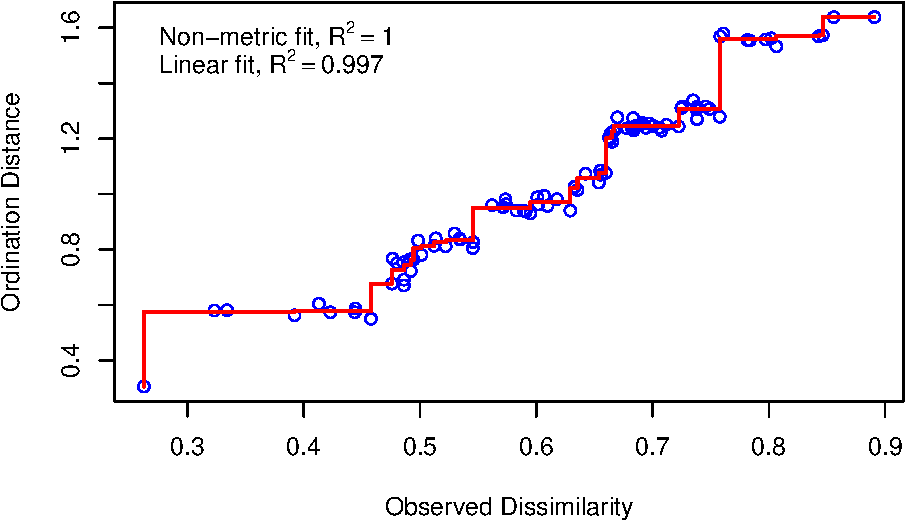
\includegraphics{log-project-aubrie-winnie_files/figure-latex/unnamed-chunk-13-1.pdf}

\begin{Shaded}
\begin{Highlighting}[]
\CommentTok{\# can test for significance of contribution of the fraction of initial treatment}
\CommentTok{\# do this with partial redundancy analysis}
\CommentTok{\# trt\_Frac\textless{}{-}rda(ass.rel.t0, init, block) \# partial rda model}
\CommentTok{\# summary(trt\_Frac) }
\CommentTok{\# RsquareAdj(trt\_Frac)$adj.r.squared \#explanatory power}
\CommentTok{\# anova.cca(trt\_Frac) \#\# this tells us if first condition, init, significantly contributes to overall variance explanation. }

\CommentTok{\# Extracting species scores and plotting }
\CommentTok{\# Species scores}
\NormalTok{species.scores}\OtherTok{\textless{}{-}}\FunctionTok{as.data.frame}\NormalTok{(vegan}\SpecialCharTok{::}\FunctionTok{scores}\NormalTok{(ass.rel.t0\_NMS,}\StringTok{"species"}\NormalTok{)) }\DocumentationTok{\#\# some species don\textquotesingle{}t have scores}
\NormalTok{species.scores}\SpecialCharTok{$}\NormalTok{species}\OtherTok{\textless{}{-}}\FunctionTok{rownames}\NormalTok{(species.scores) }

\DocumentationTok{\#\#\# NMDS 1 and 2 }
\NormalTok{log}\OtherTok{\textless{}{-}}\NormalTok{mds\_scores\_t0[mds\_scores\_t0}\SpecialCharTok{$}\NormalTok{treatment }\SpecialCharTok{==} \StringTok{"log"}\NormalTok{, ][}\FunctionTok{chull}\NormalTok{(mds\_scores\_t0[mds\_scores\_t0}\SpecialCharTok{$}\NormalTok{treatment }\SpecialCharTok{==} 
                                                          \StringTok{"log"}\NormalTok{, }\FunctionTok{c}\NormalTok{(}\StringTok{"NMDS1"}\NormalTok{, }\StringTok{"NMDS2"}\NormalTok{)]), ]}

\NormalTok{open}\OtherTok{\textless{}{-}}\NormalTok{mds\_scores\_t0[mds\_scores\_t0}\SpecialCharTok{$}\NormalTok{treatment }\SpecialCharTok{==} \StringTok{"open"}\NormalTok{, ][}\FunctionTok{chull}\NormalTok{(mds\_scores\_t0[mds\_scores\_t0}\SpecialCharTok{$}\NormalTok{treatment }\SpecialCharTok{==} 
                                                               \StringTok{"open"}\NormalTok{, }\FunctionTok{c}\NormalTok{(}\StringTok{"NMDS1"}\NormalTok{, }\StringTok{"NMDS2"}\NormalTok{)]), ]}

\NormalTok{hulldat}\OtherTok{\textless{}{-}}\FunctionTok{rbind}\NormalTok{(log,open)}

\NormalTok{nmds.plot.sp }\OtherTok{\textless{}{-}} \FunctionTok{ggplot}\NormalTok{()}\SpecialCharTok{+}
  \FunctionTok{theme\_bw}\NormalTok{()}\SpecialCharTok{+}
  \FunctionTok{theme}\NormalTok{(}\AttributeTok{panel.background =} \FunctionTok{element\_blank}\NormalTok{(),}
        \AttributeTok{panel.grid.major =} \FunctionTok{element\_blank}\NormalTok{(),  }\CommentTok{\#remove major{-}grid labels}
        \AttributeTok{panel.grid.minor =} \FunctionTok{element\_blank}\NormalTok{(),  }\CommentTok{\#remove minor{-}grid labels}
        \AttributeTok{plot.background =} \FunctionTok{element\_blank}\NormalTok{(), }
        \AttributeTok{axis.text =} \FunctionTok{element\_text}\NormalTok{(}\AttributeTok{size =} \DecValTok{10}\NormalTok{),}
        \AttributeTok{axis.title=}\FunctionTok{element\_text}\NormalTok{(}\AttributeTok{size=}\DecValTok{15}\NormalTok{),}
        \AttributeTok{legend.title=}\FunctionTok{element\_text}\NormalTok{(}\AttributeTok{size=}\DecValTok{15}\NormalTok{), }
        \AttributeTok{legend.text=}\FunctionTok{element\_text}\NormalTok{(}\AttributeTok{size=}\DecValTok{10}\NormalTok{))}\SpecialCharTok{+}
  \FunctionTok{geom\_text\_repel}\NormalTok{(}\AttributeTok{data=}\NormalTok{species.scores, }\FunctionTok{aes}\NormalTok{(NMDS1, NMDS2, }\AttributeTok{label=}\NormalTok{species), }\AttributeTok{alpha=}\FloatTok{0.9}\NormalTok{, }\AttributeTok{size=}\DecValTok{5}\NormalTok{, }\AttributeTok{col=}\StringTok{\textquotesingle{}darkgray\textquotesingle{}}\NormalTok{,}\AttributeTok{na.rm=}\ConstantTok{TRUE}\NormalTok{)}\SpecialCharTok{+}
  \FunctionTok{geom\_polygon}\NormalTok{(}\AttributeTok{data=}\NormalTok{hulldat, }\FunctionTok{aes}\NormalTok{(NMDS1, NMDS2, }\AttributeTok{fill=}\NormalTok{treatment, }\AttributeTok{group=}\NormalTok{treatment), }\AttributeTok{alpha=}\FloatTok{0.3}\NormalTok{)}\SpecialCharTok{+}
  \FunctionTok{scale\_fill\_manual}\NormalTok{(}\AttributeTok{values=}\FunctionTok{c}\NormalTok{(}\StringTok{"\#63A088"}\NormalTok{,}\StringTok{"\#56638A"}\NormalTok{), }\AttributeTok{name=}\StringTok{"Treatment"}\NormalTok{)}\SpecialCharTok{+}
  \FunctionTok{geom\_point}\NormalTok{(}\AttributeTok{data=}\NormalTok{mds\_scores\_t0, }\FunctionTok{aes}\NormalTok{(NMDS1, NMDS2, }\AttributeTok{shape=}\NormalTok{block, }\AttributeTok{col=}\NormalTok{treatment), }\AttributeTok{size=}\DecValTok{6}\NormalTok{)}\SpecialCharTok{+} 
  \FunctionTok{scale\_shape\_manual}\NormalTok{(}\AttributeTok{values =} \FunctionTok{c}\NormalTok{(}\DecValTok{14}\NormalTok{,}\DecValTok{15}\NormalTok{,}\DecValTok{16}\NormalTok{,}\DecValTok{17}\NormalTok{,}\DecValTok{11}\NormalTok{,}\DecValTok{18}\NormalTok{,}\DecValTok{8}\NormalTok{), }\AttributeTok{name=}\StringTok{\textquotesingle{}Block\textquotesingle{}}\NormalTok{)}\SpecialCharTok{+}
  \FunctionTok{scale\_colour\_manual}\NormalTok{(}\AttributeTok{values=}\FunctionTok{c}\NormalTok{(}\StringTok{"\#63A088"}\NormalTok{,}\StringTok{"\#56638A"}\NormalTok{), }\AttributeTok{name=}\StringTok{"Treatment"}\NormalTok{)}\SpecialCharTok{+}
  \FunctionTok{labs}\NormalTok{(}\AttributeTok{title=}\FunctionTok{paste0}\NormalTok{(}\StringTok{"Stress: "}\NormalTok{, }\FunctionTok{round}\NormalTok{(ass.rel.t0\_NMS}\SpecialCharTok{$}\NormalTok{stress,}\DecValTok{3}\NormalTok{)))}

\NormalTok{nmds.plot.nutrient }\OtherTok{\textless{}{-}} \FunctionTok{ggplot}\NormalTok{()}\SpecialCharTok{+}
  \FunctionTok{theme\_bw}\NormalTok{()}\SpecialCharTok{+}
  \FunctionTok{theme}\NormalTok{(}\AttributeTok{panel.background =} \FunctionTok{element\_blank}\NormalTok{(),}
        \AttributeTok{panel.grid.major =} \FunctionTok{element\_blank}\NormalTok{(),  }\CommentTok{\#remove major{-}grid labels}
        \AttributeTok{panel.grid.minor =} \FunctionTok{element\_blank}\NormalTok{(),  }\CommentTok{\#remove minor{-}grid labels}
        \AttributeTok{plot.background =} \FunctionTok{element\_blank}\NormalTok{(), }
        \AttributeTok{axis.text =} \FunctionTok{element\_text}\NormalTok{(}\AttributeTok{size =} \DecValTok{10}\NormalTok{),}
        \AttributeTok{axis.title=}\FunctionTok{element\_text}\NormalTok{(}\AttributeTok{size=}\DecValTok{15}\NormalTok{),}
        \AttributeTok{legend.title=}\FunctionTok{element\_text}\NormalTok{(}\AttributeTok{size=}\DecValTok{15}\NormalTok{), }
        \AttributeTok{legend.text=}\FunctionTok{element\_text}\NormalTok{(}\AttributeTok{size=}\DecValTok{10}\NormalTok{))}\SpecialCharTok{+}
  \FunctionTok{geom\_polygon}\NormalTok{(}\AttributeTok{data=}\NormalTok{hulldat, }\FunctionTok{aes}\NormalTok{(NMDS1, NMDS2, }\AttributeTok{fill=}\NormalTok{treatment, }\AttributeTok{group=}\NormalTok{treatment), }\AttributeTok{alpha=}\FloatTok{0.3}\NormalTok{)}\SpecialCharTok{+}
  \FunctionTok{scale\_fill\_manual}\NormalTok{(}\AttributeTok{values=}\FunctionTok{c}\NormalTok{(}\StringTok{"\#63A088"}\NormalTok{,}\StringTok{"\#56638A"}\NormalTok{), }\AttributeTok{name=}\StringTok{"Treatment"}\NormalTok{)}\SpecialCharTok{+}
  \FunctionTok{geom\_point}\NormalTok{(}\AttributeTok{data=}\NormalTok{mds\_scores\_t0, }\FunctionTok{aes}\NormalTok{(NMDS1, NMDS2, }\AttributeTok{shape=}\NormalTok{block, }\AttributeTok{col=}\NormalTok{treatment), }\AttributeTok{size=}\DecValTok{6}\NormalTok{)}\SpecialCharTok{+} 
  \FunctionTok{scale\_shape\_manual}\NormalTok{(}\AttributeTok{values =} \FunctionTok{c}\NormalTok{(}\DecValTok{14}\NormalTok{,}\DecValTok{15}\NormalTok{,}\DecValTok{16}\NormalTok{,}\DecValTok{17}\NormalTok{,}\DecValTok{11}\NormalTok{,}\DecValTok{18}\NormalTok{,}\DecValTok{8}\NormalTok{), }\AttributeTok{name=}\StringTok{\textquotesingle{}Block\textquotesingle{}}\NormalTok{)}\SpecialCharTok{+}
  \FunctionTok{scale\_colour\_manual}\NormalTok{(}\AttributeTok{values=}\FunctionTok{c}\NormalTok{(}\StringTok{"\#63A088"}\NormalTok{,}\StringTok{"\#56638A"}\NormalTok{), }\AttributeTok{name=}\StringTok{"Treatment"}\NormalTok{)}\SpecialCharTok{+}
  \FunctionTok{geom\_segment}\NormalTok{(}\FunctionTok{aes}\NormalTok{(}\AttributeTok{x =} \DecValTok{0}\NormalTok{, }\AttributeTok{y =} \DecValTok{0}\NormalTok{, }\AttributeTok{xend =}\NormalTok{ NMDS1, }\AttributeTok{yend =}\NormalTok{ NMDS2), }
       \AttributeTok{data =}\NormalTok{ en\_coord\_cont, }\AttributeTok{size =}\FloatTok{0.5}\NormalTok{, }\AttributeTok{alpha =} \FloatTok{0.5}\NormalTok{, }\AttributeTok{colour =} \StringTok{"grey30"}\NormalTok{) }\SpecialCharTok{+}
     \FunctionTok{geom\_text}\NormalTok{(}\AttributeTok{data =}\NormalTok{ en\_coord\_cont, }\FunctionTok{aes}\NormalTok{(}\AttributeTok{x =}\NormalTok{ NMDS1, }\AttributeTok{y =}\NormalTok{ NMDS2), }\AttributeTok{colour =} \StringTok{"grey30"}\NormalTok{, }
       \AttributeTok{fontface =} \StringTok{"bold"}\NormalTok{, }\AttributeTok{label =} \FunctionTok{row.names}\NormalTok{(en\_coord\_cont))}
\end{Highlighting}
\end{Shaded}

\begin{verbatim}
## Warning: Using `size` aesthetic for lines was deprecated in ggplot2 3.4.0.
## i Please use `linewidth` instead.
## This warning is displayed once every 8 hours.
## Call `lifecycle::last_lifecycle_warnings()` to see where this warning was
## generated.
\end{verbatim}

\begin{Shaded}
\begin{Highlighting}[]
\CommentTok{\# put both nmds plots together}
\NormalTok{(nmds.plot.sp }\SpecialCharTok{+} \FunctionTok{theme}\NormalTok{(}\AttributeTok{legend.position =} \StringTok{"none"}\NormalTok{)) }\SpecialCharTok{+}\NormalTok{ nmds.plot.nutrient }\SpecialCharTok{+} \FunctionTok{plot\_layout}\NormalTok{(}\AttributeTok{guides =} \StringTok{"collect"}\NormalTok{) }\SpecialCharTok{+} \FunctionTok{plot\_annotation}\NormalTok{(}\AttributeTok{title =} \StringTok{\textquotesingle{}Plant composition: 2020\textquotesingle{}}\NormalTok{)}
\end{Highlighting}
\end{Shaded}

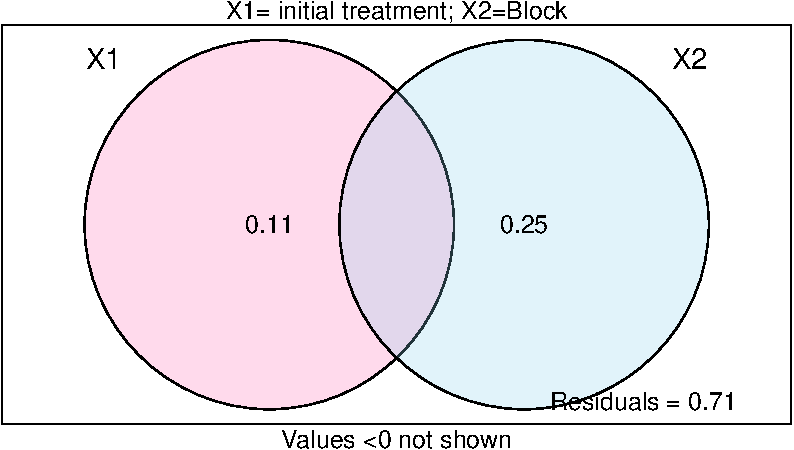
\includegraphics{log-project-aubrie-winnie_files/figure-latex/unnamed-chunk-13-2.pdf}

\emph{2021} - There is no significant correlation between nutrient
elements and plant composition.

\begin{Shaded}
\begin{Highlighting}[]
\CommentTok{\# Data wrangling}
\CommentTok{\# This data set does not include unidentified species.}
\NormalTok{comm }\OtherTok{\textless{}{-}} \FunctionTok{read.csv}\NormalTok{(}\StringTok{"20{-}22\_species\_composition\_data\_no\_unk.csv"}\NormalTok{, }\AttributeTok{header =}\NormalTok{ T)}

\CommentTok{\# Remove the locations surveyed in 2021 and 2022 that were not surveyed in 2020 {-} aka, cm=0, cm=21, cm = 22, cm = 29.}
\NormalTok{comm}\OtherTok{\textless{}{-}}\NormalTok{comm[}\FunctionTok{which}\NormalTok{(comm}\SpecialCharTok{$}\NormalTok{cm\_location}\SpecialCharTok{!=}\DecValTok{21} \SpecialCharTok{\&}\NormalTok{ comm}\SpecialCharTok{$}\NormalTok{cm\_location}\SpecialCharTok{!=}\DecValTok{0} \SpecialCharTok{\&}\NormalTok{ comm}\SpecialCharTok{$}\NormalTok{cm\_location}\SpecialCharTok{!=}\DecValTok{22} \SpecialCharTok{\&}\NormalTok{ comm}\SpecialCharTok{$}\NormalTok{cm\_location}\SpecialCharTok{!=}\DecValTok{29}\NormalTok{),]}

\CommentTok{\# Make a group name for each row}
\NormalTok{comm}\SpecialCharTok{$}\NormalTok{grp}\OtherTok{\textless{}{-}}\FunctionTok{apply}\NormalTok{(comm[}\FunctionTok{c}\NormalTok{(}\DecValTok{1}\NormalTok{,}\DecValTok{3}\NormalTok{,}\DecValTok{5}\NormalTok{,}\DecValTok{6}\NormalTok{,}\DecValTok{7}\NormalTok{)], }\DecValTok{1}\NormalTok{, paste, }\AttributeTok{collapse=}\StringTok{":"}\NormalTok{) }\CommentTok{\# timepoint, block, transect\_name, initial state}

\CommentTok{\# Need to make each row a community using matrify.}
\NormalTok{commsub}\OtherTok{\textless{}{-}}\NormalTok{comm[,}\FunctionTok{c}\NormalTok{(}\DecValTok{15}\NormalTok{,}\DecValTok{10}\NormalTok{,}\DecValTok{13}\NormalTok{)] }\CommentTok{\# group, species\_code, and count of each species for each transect. transects are rows.}
\NormalTok{commsub }\OtherTok{\textless{}{-}}\FunctionTok{as.data.frame}\NormalTok{(commsub)}
\NormalTok{commtry}\OtherTok{\textless{}{-}}\FunctionTok{matrify}\NormalTok{(commsub) }\CommentTok{\# make it an expanded species matrix }
\end{Highlighting}
\end{Shaded}

\begin{verbatim}
## Warning in matrify(commsub): NAs introduced by coercion
\end{verbatim}

\begin{Shaded}
\begin{Highlighting}[]
\NormalTok{commtry}\SpecialCharTok{$}\NormalTok{x[}\FunctionTok{which}\NormalTok{(}\FunctionTok{is.na}\NormalTok{(commtry}\SpecialCharTok{$}\NormalTok{x))] }\OtherTok{\textless{}{-}} \DecValTok{1} \CommentTok{\# "x" means that there were no individuals in the transect, but we are going to keep track of this as if it were a species}
\CommentTok{\# ncol(commtry) \# how many species are we working with in our community matrix}

\CommentTok{\# Store grouping row names as a column, then remove rownames.}
\NormalTok{commtry}\SpecialCharTok{$}\NormalTok{grps}\OtherTok{\textless{}{-}}\FunctionTok{rownames}\NormalTok{(commtry)}
\FunctionTok{rownames}\NormalTok{(commtry)}\OtherTok{\textless{}{-}}\ConstantTok{NULL}
\CommentTok{\# names(commtry)}

\CommentTok{\# Split group info into columns for each variable}
\NormalTok{mat}\OtherTok{\textless{}{-}}\FunctionTok{separate}\NormalTok{(commtry, }\DecValTok{88}\NormalTok{, }\FunctionTok{c}\NormalTok{(}\StringTok{"time"}\NormalTok{,}\StringTok{"block"}\NormalTok{,}\StringTok{"transect"}\NormalTok{,}\StringTok{"init"}\NormalTok{,}\StringTok{"treatment"}\NormalTok{), }\StringTok{":"}\NormalTok{)}
\CommentTok{\# names(mat) \#check}

\CommentTok{\# Set up nutrient analysis data}
\NormalTok{nutrient }\OtherTok{\textless{}{-}} \FunctionTok{read.csv}\NormalTok{(}\StringTok{"Nutrient.csv"}\NormalTok{, }\AttributeTok{header =}\NormalTok{ T)}
\NormalTok{nutrient }\OtherTok{\textless{}{-}}\FunctionTok{separate}\NormalTok{(nutrient,}\DecValTok{2}\NormalTok{ , }\FunctionTok{c}\NormalTok{(}\StringTok{"block"}\NormalTok{,}\StringTok{"plot"}\NormalTok{), }\StringTok{"\_"}\NormalTok{)}
\NormalTok{nutrient }\OtherTok{\textless{}{-}}\NormalTok{ nutrient[,}\DecValTok{2}\SpecialCharTok{:}\DecValTok{18}\NormalTok{]}

\CommentTok{\# subset data where all t0 communities, insitu log and insitu open communities at t1 and t2 are included.}
\NormalTok{mat2 }\OtherTok{\textless{}{-}}\NormalTok{ mat[}\FunctionTok{which}\NormalTok{(mat}\SpecialCharTok{$}\NormalTok{time}\SpecialCharTok{==}\StringTok{"t1"} \SpecialCharTok{\&}\NormalTok{  mat}\SpecialCharTok{$}\NormalTok{treatment}\SpecialCharTok{==}\StringTok{"open"} \SpecialCharTok{|}\NormalTok{ mat}\SpecialCharTok{$}\NormalTok{time}\SpecialCharTok{==}\StringTok{"t1"} \SpecialCharTok{\&}\NormalTok{ mat}\SpecialCharTok{$}\NormalTok{treatment}\SpecialCharTok{==}\StringTok{"insitu\_log"}\NormalTok{),]}
\NormalTok{mat2}\SpecialCharTok{$}\NormalTok{grp}\OtherTok{\textless{}{-}}\FunctionTok{apply}\NormalTok{(mat2[}\FunctionTok{c}\NormalTok{(}\DecValTok{89}\NormalTok{,}\DecValTok{91}\NormalTok{)], }\DecValTok{1}\NormalTok{, paste, }\AttributeTok{collapse=}\StringTok{":"}\NormalTok{) }\CommentTok{\# block, init as grouping}
\CommentTok{\# names(mat2) \#check}

\CommentTok{\# another df where the grouping variables are time, block and initial state}
\CommentTok{\# each row is a transect in a certain year.}
\NormalTok{df}\OtherTok{\textless{}{-}}\NormalTok{mat2[,}\FunctionTok{c}\NormalTok{(}\DecValTok{1}\SpecialCharTok{:}\DecValTok{87}\NormalTok{, }\DecValTok{93}\NormalTok{)]}
\NormalTok{df2 }\OtherTok{=}\NormalTok{ df }\SpecialCharTok{\%\textgreater{}\%} \FunctionTok{mutate}\NormalTok{(}\FunctionTok{across}\NormalTok{(}\AttributeTok{.cols=}\DecValTok{1}\SpecialCharTok{:}\DecValTok{87}\NormalTok{,}\AttributeTok{.fns=}\NormalTok{as.numeric)) }\CommentTok{\# make everything numeric}
\FunctionTok{rownames}\NormalTok{(df2)}\OtherTok{\textless{}{-}}\ConstantTok{NULL} \CommentTok{\# remove rownames}

\DocumentationTok{\#\# new with group vars}
\NormalTok{nublock}\OtherTok{\textless{}{-}}\FunctionTok{separate}\NormalTok{(df2, }\DecValTok{88}\NormalTok{, }\FunctionTok{c}\NormalTok{(}\StringTok{"block"}\NormalTok{, }\StringTok{"init"}\NormalTok{), }\StringTok{":"}\NormalTok{) }\CommentTok{\# just looking at time, block \& initial treatment}

\CommentTok{\# want to sum across transects in same block X init treatment}
\NormalTok{nublock}\SpecialCharTok{$}\NormalTok{sumgrp}\OtherTok{\textless{}{-}}\FunctionTok{apply}\NormalTok{(mat2[}\FunctionTok{c}\NormalTok{(}\DecValTok{89}\NormalTok{, }\DecValTok{91}\NormalTok{)], }\DecValTok{1}\NormalTok{, paste, }\AttributeTok{collapse=}\StringTok{":"}\NormalTok{)}
\CommentTok{\# head(nublock)}

\CommentTok{\# sum observations across initial X  block (group variable)}
\CommentTok{\# this gives number of plants in each transect TYPE for each year in each block. should be 2 types X 3 years X 7 blocks rows }
\NormalTok{blocksum}\OtherTok{\textless{}{-}}\FunctionTok{rowsum}\NormalTok{(nublock[,}\FunctionTok{c}\NormalTok{(}\DecValTok{1}\SpecialCharTok{:}\DecValTok{87}\NormalTok{)], }\AttributeTok{group=}\NormalTok{nublock}\SpecialCharTok{$}\NormalTok{sumgrp)}
\NormalTok{blocksum}\SpecialCharTok{$}\NormalTok{grps}\OtherTok{\textless{}{-}}\FunctionTok{rownames}\NormalTok{(blocksum)}
\FunctionTok{rownames}\NormalTok{(blocksum)}\OtherTok{\textless{}{-}}\ConstantTok{NULL} \CommentTok{\# remove rownames}
\FunctionTok{nrow}\NormalTok{(blocksum) }\CommentTok{\# it is 14 rows as expected }
\end{Highlighting}
\end{Shaded}

\begin{verbatim}
## [1] 14
\end{verbatim}

\begin{Shaded}
\begin{Highlighting}[]
\DocumentationTok{\#\# expand again}
\NormalTok{blocksum}\OtherTok{\textless{}{-}}\FunctionTok{separate}\NormalTok{(blocksum, }\DecValTok{88}\NormalTok{, }\FunctionTok{c}\NormalTok{(}\StringTok{"block"}\NormalTok{, }\StringTok{"init"}\NormalTok{), }\StringTok{":"}\NormalTok{)}
\NormalTok{nutrient\_join }\OtherTok{\textless{}{-}}\NormalTok{ nutrient[,}\FunctionTok{c}\NormalTok{(}\DecValTok{1}\NormalTok{,}\DecValTok{3}\NormalTok{,}\DecValTok{7}\SpecialCharTok{:}\DecValTok{10}\NormalTok{, }\DecValTok{12}\NormalTok{,}\DecValTok{17}\NormalTok{)]}
\NormalTok{blocksum }\OtherTok{\textless{}{-}} \FunctionTok{inner\_join}\NormalTok{(blocksum, nutrient\_join, }\AttributeTok{by =} \FunctionTok{c}\NormalTok{(}\StringTok{"init"}\NormalTok{, }\StringTok{"block"}\NormalTok{))}

\CommentTok{\# at the moment this includes where there were no plants ("x" column in matrix)}
\NormalTok{assemblies\_t1}\OtherTok{\textless{}{-}}\NormalTok{blocksum[,}\FunctionTok{c}\NormalTok{(}\DecValTok{1}\SpecialCharTok{:}\DecValTok{87}\NormalTok{)]}

\CommentTok{\# group {-} these are the treatment variables that need to be separately fed into the MDS analaysis from the community analysis.}
\NormalTok{group\_init}\OtherTok{\textless{}{-}}\NormalTok{blocksum}\SpecialCharTok{$}\NormalTok{init}
\NormalTok{group\_block}\OtherTok{\textless{}{-}}\NormalTok{blocksum}\SpecialCharTok{$}\NormalTok{block}
\NormalTok{group\_nutrient}\OtherTok{\textless{}{-}}\NormalTok{blocksum[,}\FunctionTok{c}\NormalTok{(}\DecValTok{90}\SpecialCharTok{:}\DecValTok{95}\NormalTok{)]}

\CommentTok{\# MDS }
\NormalTok{ass.rel.t1}\OtherTok{\textless{}{-}}\FunctionTok{decostand}\NormalTok{(assemblies\_t1, }\AttributeTok{method=}\StringTok{\textquotesingle{}hel\textquotesingle{}}\NormalTok{) }\CommentTok{\#standardize assemblies }
\NormalTok{ass.rel.t1\_NMS }\OtherTok{\textless{}{-}} \FunctionTok{metaMDS}\NormalTok{(ass.rel.t1, }\AttributeTok{distance =} \StringTok{\textquotesingle{}bray\textquotesingle{}}\NormalTok{, }\AttributeTok{k =} \DecValTok{4}\NormalTok{) }\CommentTok{\# run MDS }
\end{Highlighting}
\end{Shaded}

\begin{verbatim}
## Run 0 stress 0.07021466 
## Run 1 stress 0.07697598 
## Run 2 stress 0.07021459 
## ... New best solution
## ... Procrustes: rmse 0.0001945646  max resid 0.0003498818 
## ... Similar to previous best
## Run 3 stress 0.07021471 
## ... Procrustes: rmse 0.0002791863  max resid 0.0004695112 
## ... Similar to previous best
## Run 4 stress 0.07648601 
## Run 5 stress 0.08006069 
## Run 6 stress 0.07021471 
## ... Procrustes: rmse 0.0002504733  max resid 0.0004616403 
## ... Similar to previous best
## Run 7 stress 0.07021476 
## ... Procrustes: rmse 0.0003136528  max resid 0.0005275765 
## ... Similar to previous best
## Run 8 stress 0.07021473 
## ... Procrustes: rmse 0.0002662037  max resid 0.0004869097 
## ... Similar to previous best
## Run 9 stress 0.07021458 
## ... New best solution
## ... Procrustes: rmse 6.495776e-05  max resid 0.0001063562 
## ... Similar to previous best
## Run 10 stress 0.07021458 
## ... New best solution
## ... Procrustes: rmse 3.078454e-05  max resid 6.632422e-05 
## ... Similar to previous best
## Run 11 stress 0.07021463 
## ... Procrustes: rmse 0.0001353704  max resid 0.0002563599 
## ... Similar to previous best
## Run 12 stress 0.07021457 
## ... New best solution
## ... Procrustes: rmse 3.116454e-05  max resid 5.325305e-05 
## ... Similar to previous best
## Run 13 stress 0.08006058 
## Run 14 stress 0.07021463 
## ... Procrustes: rmse 0.0001245778  max resid 0.0002246657 
## ... Similar to previous best
## Run 15 stress 0.07647571 
## Run 16 stress 0.07647534 
## Run 17 stress 0.07647496 
## Run 18 stress 0.1018298 
## Run 19 stress 0.07021463 
## ... Procrustes: rmse 0.000151352  max resid 0.0002948416 
## ... Similar to previous best
## Run 20 stress 0.0702147 
## ... Procrustes: rmse 0.0002262462  max resid 0.0004090218 
## ... Similar to previous best
## *** Best solution repeated 4 times
\end{verbatim}

\begin{Shaded}
\begin{Highlighting}[]
\CommentTok{\# stressplot(ass.rel.t1\_NMS) \# check fit}
\NormalTok{en.nutrient }\OtherTok{=} \FunctionTok{envfit}\NormalTok{(ass.rel.t1\_NMS, group\_nutrient, }\AttributeTok{permutations =} \DecValTok{999}\NormalTok{, }\AttributeTok{na.rm =} \ConstantTok{TRUE}\NormalTok{)}
\CommentTok{\# plot(ass.rel.t1\_NMS) }
\CommentTok{\# plot(en.nutrient)}
\FunctionTok{print}\NormalTok{(en.nutrient) }\DocumentationTok{\#\#\#\#\#\#\#\#\#\# it is basically saying most of the nutrient does not affect the composition of plants.}
\end{Highlighting}
\end{Shaded}

\begin{verbatim}
## 
## ***VECTORS
## 
##        NMDS1    NMDS2     r2 Pr(>r)
## N    0.44546 -0.89530 0.3457  0.102
## P   -0.86872  0.49531 0.1385  0.447
## K   -0.75129  0.65997 0.1268  0.465
## C    0.84943 -0.52771 0.0169  0.910
## pH  -0.92568 -0.37830 0.3009  0.151
## CEC -0.88034 -0.47435 0.0770  0.661
## Permutation: free
## Number of permutations: 999
\end{verbatim}

\begin{Shaded}
\begin{Highlighting}[]
\CommentTok{\# scores}
\NormalTok{mds\_scores\_t1}\OtherTok{\textless{}{-}}\FunctionTok{as.data.frame}\NormalTok{(vegan}\SpecialCharTok{::}\FunctionTok{scores}\NormalTok{(ass.rel.t1\_NMS)}\SpecialCharTok{$}\NormalTok{sites) }\CommentTok{\# extract scores}
\NormalTok{mds\_scores\_t1}\SpecialCharTok{$}\NormalTok{site}\OtherTok{\textless{}{-}}\FunctionTok{rownames}\NormalTok{(vegan}\SpecialCharTok{::}\FunctionTok{scores}\NormalTok{(ass.rel.t1\_NMS)}\SpecialCharTok{$}\NormalTok{sites) }\CommentTok{\# extract names }
\NormalTok{mds\_scores\_t1}\SpecialCharTok{$}\NormalTok{treatment}\OtherTok{\textless{}{-}}\NormalTok{group\_init }\CommentTok{\# grouping factor 1 }
\NormalTok{mds\_scores\_t1}\SpecialCharTok{$}\NormalTok{block}\OtherTok{\textless{}{-}}\NormalTok{group\_block }\CommentTok{\# grouping factor 2 }
\NormalTok{en\_coord\_cont }\OtherTok{=} \FunctionTok{as.data.frame}\NormalTok{(vegan}\SpecialCharTok{::}\FunctionTok{scores}\NormalTok{(en.nutrient, }\StringTok{"vectors"}\NormalTok{)) }\SpecialCharTok{*} \FunctionTok{ordiArrowMul}\NormalTok{(en.nutrient)}

\CommentTok{\# explaining factors}
\NormalTok{init}\OtherTok{\textless{}{-}}\FunctionTok{as.factor}\NormalTok{(group\_init) }\CommentTok{\# grouping factor 1{-} convert to factor}
\NormalTok{block}\OtherTok{\textless{}{-}}\FunctionTok{as.factor}\NormalTok{(group\_block) }\CommentTok{\# grouping factor 2{-} convert to factor}

\DocumentationTok{\#\#\#\# rda model analysis \& results \#\#\#\# }
\CommentTok{\# can look at significance of model where initial treatment and block explain variation in community}
\CommentTok{\# trt\_tot\_2\textless{}{-}rda(ass.rel.t1\textasciitilde{}init+block) \# run model using standardized data }
\CommentTok{\# summary(trt\_tot\_2)}
\CommentTok{\# anova.cca(trt\_tot\_2, step=1000, by="term") \#\# test for model significance}

\CommentTok{\# can model using varpart to look at contributions of initial treatment and block}
\NormalTok{var.mod2}\OtherTok{\textless{}{-}}\FunctionTok{varpart}\NormalTok{(ass.rel.t1, init, block) }\CommentTok{\# run model on standardized data}
\FunctionTok{plot}\NormalTok{(var.mod2, }\AttributeTok{bg=}\FunctionTok{c}\NormalTok{(}\StringTok{"hotpink"}\NormalTok{,}\StringTok{"skyblue"}\NormalTok{))}
\FunctionTok{mtext}\NormalTok{(}\StringTok{"X1= Treatment; X2=Block"}\NormalTok{, }\AttributeTok{side=}\DecValTok{3}\NormalTok{)}
\end{Highlighting}
\end{Shaded}

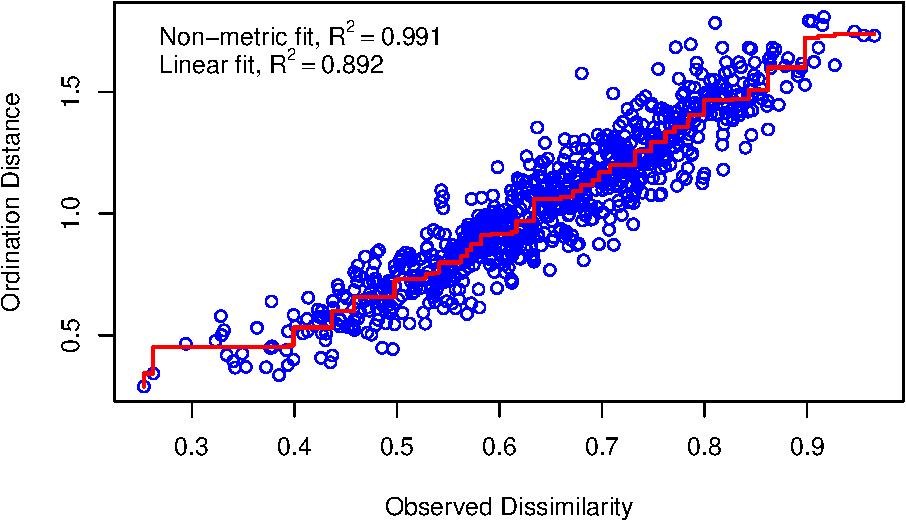
\includegraphics{log-project-aubrie-winnie_files/figure-latex/unnamed-chunk-14-1.pdf}

\begin{Shaded}
\begin{Highlighting}[]
\DocumentationTok{\#\# can test for significance of contribution of the fraction of initial treatment}
\CommentTok{\# do this with partial redundancy analysis}
\CommentTok{\# trt\_Frac\textless{}{-}rda(ass.rel.t1, init, block) \# partial rda model}
\CommentTok{\# summary(trt\_Frac) }
\CommentTok{\# RsquareAdj(trt\_Frac)$adj.r.squared \#explanatory power}
\CommentTok{\# anova.cca(trt\_Frac) \#\# this tells us if first condition, init, significantly contributes to overall variance explanation. }

\DocumentationTok{\#\#\# extracting species scores and plotting }
\CommentTok{\# species scores}
\NormalTok{species.scores}\OtherTok{\textless{}{-}}\FunctionTok{as.data.frame}\NormalTok{(vegan}\SpecialCharTok{::}\FunctionTok{scores}\NormalTok{(ass.rel.t1\_NMS,}\StringTok{"species"}\NormalTok{)) }\DocumentationTok{\#\# some species don\textquotesingle{}t have scores}
\NormalTok{species.scores}\SpecialCharTok{$}\NormalTok{species}\OtherTok{\textless{}{-}}\FunctionTok{rownames}\NormalTok{(species.scores) }

\DocumentationTok{\#\#\# NMDS 1 and 2 }
\NormalTok{log}\OtherTok{\textless{}{-}}\NormalTok{mds\_scores\_t1[mds\_scores\_t1}\SpecialCharTok{$}\NormalTok{treatment }\SpecialCharTok{==} \StringTok{"log"}\NormalTok{, ][}\FunctionTok{chull}\NormalTok{(mds\_scores\_t1[mds\_scores\_t1}\SpecialCharTok{$}\NormalTok{treatment }\SpecialCharTok{==} 
                                                          \StringTok{"log"}\NormalTok{, }\FunctionTok{c}\NormalTok{(}\StringTok{"NMDS1"}\NormalTok{, }\StringTok{"NMDS2"}\NormalTok{)]), ]}

\NormalTok{open}\OtherTok{\textless{}{-}}\NormalTok{mds\_scores\_t1[mds\_scores\_t1}\SpecialCharTok{$}\NormalTok{treatment }\SpecialCharTok{==} \StringTok{"open"}\NormalTok{, ][}\FunctionTok{chull}\NormalTok{(mds\_scores\_t1[mds\_scores\_t1}\SpecialCharTok{$}\NormalTok{treatment }\SpecialCharTok{==} 
                                                               \StringTok{"open"}\NormalTok{, }\FunctionTok{c}\NormalTok{(}\StringTok{"NMDS1"}\NormalTok{, }\StringTok{"NMDS2"}\NormalTok{)]), ]}

\NormalTok{hulldat}\OtherTok{\textless{}{-}}\FunctionTok{rbind}\NormalTok{(log,open)}

\NormalTok{nmds.plot.sp }\OtherTok{\textless{}{-}} \FunctionTok{ggplot}\NormalTok{()}\SpecialCharTok{+}
  \FunctionTok{theme\_bw}\NormalTok{()}\SpecialCharTok{+}
  \FunctionTok{theme}\NormalTok{(}\AttributeTok{panel.background =} \FunctionTok{element\_blank}\NormalTok{(),}
        \AttributeTok{panel.grid.major =} \FunctionTok{element\_blank}\NormalTok{(),  }\CommentTok{\#remove major{-}grid labels}
        \AttributeTok{panel.grid.minor =} \FunctionTok{element\_blank}\NormalTok{(),  }\CommentTok{\#remove minor{-}grid labels}
        \AttributeTok{plot.background =} \FunctionTok{element\_blank}\NormalTok{(), }
        \AttributeTok{axis.text =} \FunctionTok{element\_text}\NormalTok{(}\AttributeTok{size =} \DecValTok{15}\NormalTok{),}
        \AttributeTok{axis.title=}\FunctionTok{element\_text}\NormalTok{(}\AttributeTok{size=}\DecValTok{20}\NormalTok{),}
        \AttributeTok{legend.title=}\FunctionTok{element\_text}\NormalTok{(}\AttributeTok{size=}\DecValTok{20}\NormalTok{), }
        \AttributeTok{legend.text=}\FunctionTok{element\_text}\NormalTok{(}\AttributeTok{size=}\DecValTok{15}\NormalTok{))}\SpecialCharTok{+}
  \FunctionTok{geom\_text\_repel}\NormalTok{(}\AttributeTok{data=}\NormalTok{species.scores, }\FunctionTok{aes}\NormalTok{(NMDS1, NMDS2, }\AttributeTok{label=}\NormalTok{species), }\AttributeTok{alpha=}\FloatTok{0.9}\NormalTok{, }\AttributeTok{size=}\DecValTok{5}\NormalTok{, }\AttributeTok{col=}\StringTok{\textquotesingle{}darkgray\textquotesingle{}}\NormalTok{,}\AttributeTok{na.rm=}\ConstantTok{TRUE}\NormalTok{)}\SpecialCharTok{+}
  \FunctionTok{geom\_polygon}\NormalTok{(}\AttributeTok{data=}\NormalTok{hulldat, }\FunctionTok{aes}\NormalTok{(NMDS1, NMDS2, }\AttributeTok{fill=}\NormalTok{treatment, }\AttributeTok{group=}\NormalTok{treatment), }\AttributeTok{alpha=}\FloatTok{0.3}\NormalTok{)}\SpecialCharTok{+}\FunctionTok{scale\_fill\_manual}\NormalTok{(}\AttributeTok{values=}\FunctionTok{c}\NormalTok{(}\StringTok{"\#63A088"}\NormalTok{,}\StringTok{"\#56638A"}\NormalTok{), }\AttributeTok{name=}\StringTok{"Treatment"}\NormalTok{)}\SpecialCharTok{+}
  \FunctionTok{geom\_point}\NormalTok{(}\AttributeTok{data=}\NormalTok{mds\_scores\_t1, }\FunctionTok{aes}\NormalTok{(NMDS1, NMDS2, }\AttributeTok{shape=}\NormalTok{block, }\AttributeTok{col=}\NormalTok{treatment), }\AttributeTok{size=}\DecValTok{6}\NormalTok{)}\SpecialCharTok{+} \FunctionTok{scale\_shape\_manual}\NormalTok{(}\AttributeTok{values =} \FunctionTok{c}\NormalTok{(}\DecValTok{14}\NormalTok{,}\DecValTok{15}\NormalTok{,}\DecValTok{16}\NormalTok{,}\DecValTok{17}\NormalTok{,}\DecValTok{11}\NormalTok{,}\DecValTok{18}\NormalTok{,}\DecValTok{8}\NormalTok{), }\AttributeTok{name=}\StringTok{\textquotesingle{}Block\textquotesingle{}}\NormalTok{)}\SpecialCharTok{+}
  \FunctionTok{scale\_colour\_manual}\NormalTok{(}\AttributeTok{values=}\FunctionTok{c}\NormalTok{(}\StringTok{"\#63A088"}\NormalTok{,}\StringTok{"\#56638A"}\NormalTok{), }\AttributeTok{name=}\StringTok{"Treatment"}\NormalTok{)}\SpecialCharTok{+}
  \FunctionTok{labs}\NormalTok{(}\AttributeTok{title=}\FunctionTok{paste0}\NormalTok{(}\StringTok{"Stress: "}\NormalTok{, }\FunctionTok{round}\NormalTok{(ass.rel.t1\_NMS}\SpecialCharTok{$}\NormalTok{stress,}\DecValTok{3}\NormalTok{)))}

\NormalTok{nmds.plot.nutrient }\OtherTok{\textless{}{-}} \FunctionTok{ggplot}\NormalTok{()}\SpecialCharTok{+}
  \FunctionTok{theme\_bw}\NormalTok{()}\SpecialCharTok{+}
  \FunctionTok{theme}\NormalTok{(}\AttributeTok{panel.background =} \FunctionTok{element\_blank}\NormalTok{(),}
        \AttributeTok{panel.grid.major =} \FunctionTok{element\_blank}\NormalTok{(),  }\CommentTok{\#remove major{-}grid labels}
        \AttributeTok{panel.grid.minor =} \FunctionTok{element\_blank}\NormalTok{(),  }\CommentTok{\#remove minor{-}grid labels}
        \AttributeTok{plot.background =} \FunctionTok{element\_blank}\NormalTok{(), }
        \AttributeTok{axis.text =} \FunctionTok{element\_text}\NormalTok{(}\AttributeTok{size =} \DecValTok{15}\NormalTok{),}
        \AttributeTok{axis.title=}\FunctionTok{element\_text}\NormalTok{(}\AttributeTok{size=}\DecValTok{20}\NormalTok{),}
        \AttributeTok{legend.title=}\FunctionTok{element\_text}\NormalTok{(}\AttributeTok{size=}\DecValTok{20}\NormalTok{), }
        \AttributeTok{legend.text=}\FunctionTok{element\_text}\NormalTok{(}\AttributeTok{size=}\DecValTok{15}\NormalTok{))}\SpecialCharTok{+}
  \FunctionTok{geom\_polygon}\NormalTok{(}\AttributeTok{data=}\NormalTok{hulldat, }\FunctionTok{aes}\NormalTok{(NMDS1, NMDS2, }\AttributeTok{fill=}\NormalTok{treatment, }\AttributeTok{group=}\NormalTok{treatment), }\AttributeTok{alpha=}\FloatTok{0.3}\NormalTok{)}\SpecialCharTok{+}
  \FunctionTok{scale\_fill\_manual}\NormalTok{(}\AttributeTok{values=}\FunctionTok{c}\NormalTok{(}\StringTok{"\#63A088"}\NormalTok{,}\StringTok{"\#56638A"}\NormalTok{), }\AttributeTok{name=}\StringTok{"Treatment"}\NormalTok{)}\SpecialCharTok{+}
  \FunctionTok{geom\_point}\NormalTok{(}\AttributeTok{data=}\NormalTok{mds\_scores\_t1, }\FunctionTok{aes}\NormalTok{(NMDS1, NMDS2, }\AttributeTok{shape=}\NormalTok{block, }\AttributeTok{col=}\NormalTok{treatment), }\AttributeTok{size=}\DecValTok{6}\NormalTok{)}\SpecialCharTok{+} 
  \FunctionTok{scale\_shape\_manual}\NormalTok{(}\AttributeTok{values =} \FunctionTok{c}\NormalTok{(}\DecValTok{14}\NormalTok{,}\DecValTok{15}\NormalTok{,}\DecValTok{16}\NormalTok{,}\DecValTok{17}\NormalTok{,}\DecValTok{11}\NormalTok{,}\DecValTok{18}\NormalTok{,}\DecValTok{8}\NormalTok{), }\AttributeTok{name=}\StringTok{\textquotesingle{}Block\textquotesingle{}}\NormalTok{)}\SpecialCharTok{+}
  \FunctionTok{scale\_colour\_manual}\NormalTok{(}\AttributeTok{values=}\FunctionTok{c}\NormalTok{(}\StringTok{"\#63A088"}\NormalTok{,}\StringTok{"\#56638A"}\NormalTok{), }\AttributeTok{name=}\StringTok{"Treatment"}\NormalTok{)}\SpecialCharTok{+}
  \FunctionTok{geom\_segment}\NormalTok{(}\FunctionTok{aes}\NormalTok{(}\AttributeTok{x =} \DecValTok{0}\NormalTok{, }\AttributeTok{y =} \DecValTok{0}\NormalTok{, }\AttributeTok{xend =}\NormalTok{ NMDS1, }\AttributeTok{yend =}\NormalTok{ NMDS2), }
       \AttributeTok{data =}\NormalTok{ en\_coord\_cont, }\AttributeTok{size =}\FloatTok{0.5}\NormalTok{, }\AttributeTok{alpha =} \FloatTok{0.5}\NormalTok{, }\AttributeTok{colour =} \StringTok{"grey30"}\NormalTok{) }\SpecialCharTok{+}
     \FunctionTok{geom\_text}\NormalTok{(}\AttributeTok{data =}\NormalTok{ en\_coord\_cont, }\FunctionTok{aes}\NormalTok{(}\AttributeTok{x =}\NormalTok{ NMDS1, }\AttributeTok{y =}\NormalTok{ NMDS2), }\AttributeTok{colour =} \StringTok{"grey30"}\NormalTok{, }
       \AttributeTok{fontface =} \StringTok{"bold"}\NormalTok{, }\AttributeTok{label =} \FunctionTok{row.names}\NormalTok{(en\_coord\_cont))}\SpecialCharTok{+}
  \FunctionTok{labs}\NormalTok{(}\AttributeTok{title=}\FunctionTok{paste0}\NormalTok{(}\StringTok{"Stress: "}\NormalTok{, }\FunctionTok{round}\NormalTok{(ass.rel.t1\_NMS}\SpecialCharTok{$}\NormalTok{stress,}\DecValTok{3}\NormalTok{)))}
  
\NormalTok{(nmds.plot.sp }\SpecialCharTok{+} \FunctionTok{theme}\NormalTok{(}\AttributeTok{legend.position =} \StringTok{"none"}\NormalTok{)) }\SpecialCharTok{+}\NormalTok{ nmds.plot.nutrient }\SpecialCharTok{+} \FunctionTok{plot\_layout}\NormalTok{(}\AttributeTok{guides =} \StringTok{"collect"}\NormalTok{) }\SpecialCharTok{+} \FunctionTok{plot\_annotation}\NormalTok{(}\AttributeTok{title =} \StringTok{\textquotesingle{}Plant composition: 2020\textquotesingle{}}\NormalTok{)}
\end{Highlighting}
\end{Shaded}

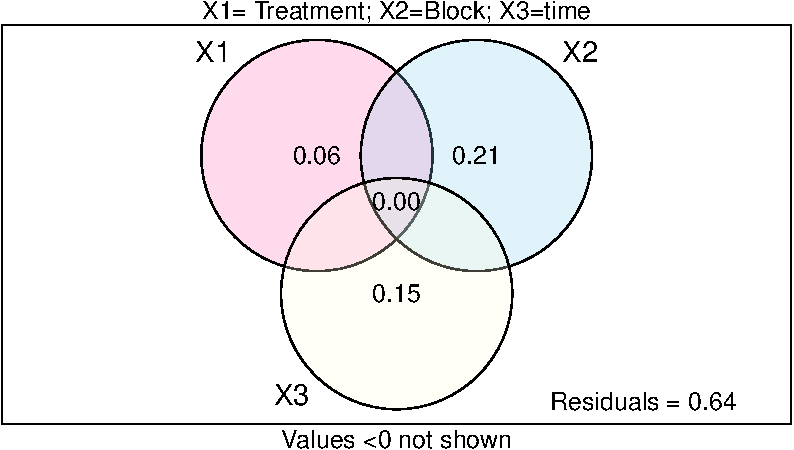
\includegraphics{log-project-aubrie-winnie_files/figure-latex/unnamed-chunk-14-2.pdf}

\emph{2022} - There is no significant correlation between nutrient
elements and plant composition.

\begin{Shaded}
\begin{Highlighting}[]
\CommentTok{\# Data wrangling}
\CommentTok{\# This data set does not include unknown data.}
\NormalTok{comm }\OtherTok{\textless{}{-}} \FunctionTok{read.csv}\NormalTok{(}\StringTok{"20{-}22\_species\_composition\_data\_no\_unk.csv"}\NormalTok{, }\AttributeTok{header =}\NormalTok{ T)}

\CommentTok{\# Remove the locations surveyed in 2021 and 2022 that were not surveyed in 2020 {-} aka, cm=0, cm=21, cm = 22, cm = 29.}
\NormalTok{comm}\OtherTok{\textless{}{-}}\NormalTok{comm[}\FunctionTok{which}\NormalTok{(comm}\SpecialCharTok{$}\NormalTok{cm\_location}\SpecialCharTok{!=}\DecValTok{21} \SpecialCharTok{\&}\NormalTok{ comm}\SpecialCharTok{$}\NormalTok{cm\_location}\SpecialCharTok{!=}\DecValTok{0} \SpecialCharTok{\&}\NormalTok{ comm}\SpecialCharTok{$}\NormalTok{cm\_location}\SpecialCharTok{!=}\DecValTok{22} \SpecialCharTok{\&}\NormalTok{ comm}\SpecialCharTok{$}\NormalTok{cm\_location}\SpecialCharTok{!=}\DecValTok{29}\NormalTok{),]}

\CommentTok{\# Make a group name for each row}
\NormalTok{comm}\SpecialCharTok{$}\NormalTok{grp}\OtherTok{\textless{}{-}}\FunctionTok{apply}\NormalTok{(comm[}\FunctionTok{c}\NormalTok{(}\DecValTok{1}\NormalTok{,}\DecValTok{3}\NormalTok{,}\DecValTok{5}\NormalTok{,}\DecValTok{6}\NormalTok{,}\DecValTok{7}\NormalTok{)], }\DecValTok{1}\NormalTok{, paste, }\AttributeTok{collapse=}\StringTok{":"}\NormalTok{) }\CommentTok{\# timepoint, block, transect\_name, initial state}

\CommentTok{\# Need to make each row a community using matrify.}
\NormalTok{commsub}\OtherTok{\textless{}{-}}\NormalTok{comm[,}\FunctionTok{c}\NormalTok{(}\DecValTok{15}\NormalTok{,}\DecValTok{10}\NormalTok{,}\DecValTok{13}\NormalTok{)] }\CommentTok{\# group, species\_code, and count of each species for each transect. transects are rows.}
\NormalTok{commsub }\OtherTok{\textless{}{-}}\FunctionTok{as.data.frame}\NormalTok{(commsub)}
\NormalTok{commtry}\OtherTok{\textless{}{-}}\FunctionTok{matrify}\NormalTok{(commsub) }\CommentTok{\# make it an expanded species matrix }
\NormalTok{commtry}\SpecialCharTok{$}\NormalTok{x[}\FunctionTok{which}\NormalTok{(}\FunctionTok{is.na}\NormalTok{(commtry}\SpecialCharTok{$}\NormalTok{x))] }\OtherTok{\textless{}{-}} \DecValTok{1} \CommentTok{\# "x" means that there were no individuals in the transect, but we are going to keep track of this as if it were a species}
\FunctionTok{ncol}\NormalTok{(commtry) }\CommentTok{\# how many species are we working with in our community matrix}
\end{Highlighting}
\end{Shaded}

\begin{verbatim}
## [1] 87
\end{verbatim}

\begin{Shaded}
\begin{Highlighting}[]
\CommentTok{\# Store grouping row names as a column, then remove rownames.}
\NormalTok{commtry}\SpecialCharTok{$}\NormalTok{grps}\OtherTok{\textless{}{-}}\FunctionTok{rownames}\NormalTok{(commtry)}
\FunctionTok{rownames}\NormalTok{(commtry)}\OtherTok{\textless{}{-}}\ConstantTok{NULL}
\FunctionTok{names}\NormalTok{(commtry)}
\end{Highlighting}
\end{Shaded}

\begin{verbatim}
##  [1] "acul"  "aicu"  "arca"  "ardy"  "arsp"  "auel"  "bldr"  "blrd"  "brdi" 
## [10] "brdr"  "brpe"  "brru"  "buse"  "caer"  "cagr"  "cahi"  "casp"  "cear" 
## [19] "chau"  "chei"  "chps"  "crcl"  "crco"  "cusc"  "cusp"  "dagl"  "dosp" 
## [28] "ento"  "erau"  "ercy"  "erra"  "ersp"  "gite"  "gnte"  "gobe"  "gocy" 
## [37] "gono"  "goro"  "gosp"  "haod"  "hygl"  "hypi"  "hypo"  "jubu"  "laro" 
## [46] "ledu"  "lele"  "loef"  "misp"  "mite"  "momo"  "mopa"  "niro"  "omco" 
## [55] "orsp"  "pala"  "peai"  "pedu"  "phsu"  "plde"  "poar"  "poca"  "pocap"
## [64] "poce"  "pogn"  "pole"  "pomu"  "pter"  "ptga"  "ptob"  "rhla"  "rhpy" 
## [73] "rhsp"  "ry"    "scna"  "sino"  "sool"  "stfi"  "stpi"  "thma"  "trcy" 
## [82] "tris"  "tror"  "trpi"  "waac"  "wagr"  "x"     "grps"
\end{verbatim}

\begin{Shaded}
\begin{Highlighting}[]
\CommentTok{\# Split group info into columns for each variable}
\NormalTok{mat}\OtherTok{\textless{}{-}}\FunctionTok{separate}\NormalTok{(commtry, }\DecValTok{88}\NormalTok{, }\FunctionTok{c}\NormalTok{(}\StringTok{"time"}\NormalTok{,}\StringTok{"block"}\NormalTok{,}\StringTok{"transect"}\NormalTok{,}\StringTok{"init"}\NormalTok{,}\StringTok{"treatment"}\NormalTok{), }\StringTok{":"}\NormalTok{)}
\FunctionTok{names}\NormalTok{(mat) }\CommentTok{\#check}
\end{Highlighting}
\end{Shaded}

\begin{verbatim}
##  [1] "acul"      "aicu"      "arca"      "ardy"      "arsp"      "auel"     
##  [7] "bldr"      "blrd"      "brdi"      "brdr"      "brpe"      "brru"     
## [13] "buse"      "caer"      "cagr"      "cahi"      "casp"      "cear"     
## [19] "chau"      "chei"      "chps"      "crcl"      "crco"      "cusc"     
## [25] "cusp"      "dagl"      "dosp"      "ento"      "erau"      "ercy"     
## [31] "erra"      "ersp"      "gite"      "gnte"      "gobe"      "gocy"     
## [37] "gono"      "goro"      "gosp"      "haod"      "hygl"      "hypi"     
## [43] "hypo"      "jubu"      "laro"      "ledu"      "lele"      "loef"     
## [49] "misp"      "mite"      "momo"      "mopa"      "niro"      "omco"     
## [55] "orsp"      "pala"      "peai"      "pedu"      "phsu"      "plde"     
## [61] "poar"      "poca"      "pocap"     "poce"      "pogn"      "pole"     
## [67] "pomu"      "pter"      "ptga"      "ptob"      "rhla"      "rhpy"     
## [73] "rhsp"      "ry"        "scna"      "sino"      "sool"      "stfi"     
## [79] "stpi"      "thma"      "trcy"      "tris"      "tror"      "trpi"     
## [85] "waac"      "wagr"      "x"         "time"      "block"     "transect" 
## [91] "init"      "treatment"
\end{verbatim}

\begin{Shaded}
\begin{Highlighting}[]
\CommentTok{\# Set up nutrient analysis data}
\NormalTok{nutrient }\OtherTok{\textless{}{-}} \FunctionTok{read.csv}\NormalTok{(}\StringTok{"Nutrient.csv"}\NormalTok{, }\AttributeTok{header =}\NormalTok{ T)}
\NormalTok{nutrient }\OtherTok{\textless{}{-}}\FunctionTok{separate}\NormalTok{(nutrient,}\DecValTok{2}\NormalTok{ , }\FunctionTok{c}\NormalTok{(}\StringTok{"block"}\NormalTok{,}\StringTok{"plot"}\NormalTok{), }\StringTok{"\_"}\NormalTok{)}
\NormalTok{nutrient }\OtherTok{\textless{}{-}}\NormalTok{ nutrient[,}\DecValTok{2}\SpecialCharTok{:}\DecValTok{18}\NormalTok{]}

\DocumentationTok{\#\#\#\#\#}
\CommentTok{\# subset data where all t0 communities, insitu log and insitu open communities at t1 and t2 are included.}
\NormalTok{mat2 }\OtherTok{\textless{}{-}}\NormalTok{ mat[}\FunctionTok{which}\NormalTok{(mat}\SpecialCharTok{$}\NormalTok{time}\SpecialCharTok{==}\StringTok{"t2"} \SpecialCharTok{\&}\NormalTok{  mat}\SpecialCharTok{$}\NormalTok{treatment}\SpecialCharTok{==}\StringTok{"open"} \SpecialCharTok{|}\NormalTok{ mat}\SpecialCharTok{$}\NormalTok{time}\SpecialCharTok{==}\StringTok{"t2"} \SpecialCharTok{\&}\NormalTok{ mat}\SpecialCharTok{$}\NormalTok{treatment}\SpecialCharTok{==}\StringTok{"insitu\_log"}\NormalTok{),]}
\NormalTok{mat2}\SpecialCharTok{$}\NormalTok{grp}\OtherTok{\textless{}{-}}\FunctionTok{apply}\NormalTok{(mat2[}\FunctionTok{c}\NormalTok{(}\DecValTok{89}\NormalTok{,}\DecValTok{91}\NormalTok{)], }\DecValTok{1}\NormalTok{, paste, }\AttributeTok{collapse=}\StringTok{":"}\NormalTok{) }\CommentTok{\# block, init as grouping}
\CommentTok{\# names(mat2) \#check}

\CommentTok{\# another df where the grouping variables are time, block and initial state}
\CommentTok{\# each row is a transect in a certain year.}
\NormalTok{df}\OtherTok{\textless{}{-}}\NormalTok{mat2[,}\FunctionTok{c}\NormalTok{(}\DecValTok{1}\SpecialCharTok{:}\DecValTok{87}\NormalTok{, }\DecValTok{93}\NormalTok{)]}
\NormalTok{df2 }\OtherTok{=}\NormalTok{ df }\SpecialCharTok{\%\textgreater{}\%} \FunctionTok{mutate}\NormalTok{(}\FunctionTok{across}\NormalTok{(}\AttributeTok{.cols=}\DecValTok{1}\SpecialCharTok{:}\DecValTok{87}\NormalTok{,}\AttributeTok{.fns=}\NormalTok{as.numeric)) }\CommentTok{\# make everything numeric}
\FunctionTok{rownames}\NormalTok{(df2)}\OtherTok{\textless{}{-}}\ConstantTok{NULL} \CommentTok{\# remove rownames}

\DocumentationTok{\#\# new with group vars}
\NormalTok{nublock}\OtherTok{\textless{}{-}}\FunctionTok{separate}\NormalTok{(df2, }\DecValTok{88}\NormalTok{, }\FunctionTok{c}\NormalTok{(}\StringTok{"block"}\NormalTok{, }\StringTok{"init"}\NormalTok{), }\StringTok{":"}\NormalTok{) }\CommentTok{\# just looking at time, block \& initial treatment}

\CommentTok{\# want to sum across transects in same block X init treatment}
\NormalTok{nublock}\SpecialCharTok{$}\NormalTok{sumgrp}\OtherTok{\textless{}{-}}\FunctionTok{apply}\NormalTok{(mat2[}\FunctionTok{c}\NormalTok{(}\DecValTok{89}\NormalTok{, }\DecValTok{91}\NormalTok{)], }\DecValTok{1}\NormalTok{, paste, }\AttributeTok{collapse=}\StringTok{":"}\NormalTok{)}
\CommentTok{\# head(nublock)}

\CommentTok{\# sum observations across initial X  block (group variable)}
\CommentTok{\# this gives number of plants in each transect TYPE for each year in each block. should be 2 types X 3 years X 7 blocks rows }
\NormalTok{blocksum}\OtherTok{\textless{}{-}}\FunctionTok{rowsum}\NormalTok{(nublock[,}\FunctionTok{c}\NormalTok{(}\DecValTok{1}\SpecialCharTok{:}\DecValTok{87}\NormalTok{)], }\AttributeTok{group=}\NormalTok{nublock}\SpecialCharTok{$}\NormalTok{sumgrp)}
\NormalTok{blocksum}\SpecialCharTok{$}\NormalTok{grps}\OtherTok{\textless{}{-}}\FunctionTok{rownames}\NormalTok{(blocksum)}
\FunctionTok{rownames}\NormalTok{(blocksum)}\OtherTok{\textless{}{-}}\ConstantTok{NULL} \CommentTok{\# remove rownames}
\CommentTok{\# nrow(blocksum) \# it is 14 rows as expected }

\DocumentationTok{\#\# expand again}
\NormalTok{blocksum}\OtherTok{\textless{}{-}}\FunctionTok{separate}\NormalTok{(blocksum, }\DecValTok{88}\NormalTok{, }\FunctionTok{c}\NormalTok{(}\StringTok{"block"}\NormalTok{, }\StringTok{"init"}\NormalTok{), }\StringTok{":"}\NormalTok{)}
\NormalTok{nutrient\_join }\OtherTok{\textless{}{-}}\NormalTok{ nutrient[,}\FunctionTok{c}\NormalTok{(}\DecValTok{1}\NormalTok{,}\DecValTok{3}\NormalTok{,}\DecValTok{7}\SpecialCharTok{:}\DecValTok{10}\NormalTok{, }\DecValTok{12}\NormalTok{,}\DecValTok{17}\NormalTok{)]}
\NormalTok{blocksum }\OtherTok{\textless{}{-}} \FunctionTok{inner\_join}\NormalTok{(blocksum, nutrient\_join, }\AttributeTok{by =} \FunctionTok{c}\NormalTok{(}\StringTok{"init"}\NormalTok{, }\StringTok{"block"}\NormalTok{))}

\CommentTok{\# at the moment this includes where there were no plants ("x" column in matrix)}
\NormalTok{assemblies\_t2}\OtherTok{\textless{}{-}}\NormalTok{blocksum[,}\FunctionTok{c}\NormalTok{(}\DecValTok{1}\SpecialCharTok{:}\DecValTok{87}\NormalTok{)]}

\CommentTok{\# group {-} these are the treatment variables that need to be separately fed into the MDS analaysis from the community analysis.}
\NormalTok{group\_init}\OtherTok{\textless{}{-}}\NormalTok{blocksum}\SpecialCharTok{$}\NormalTok{init}
\NormalTok{group\_block}\OtherTok{\textless{}{-}}\NormalTok{blocksum}\SpecialCharTok{$}\NormalTok{block}
\NormalTok{group\_nutrient}\OtherTok{\textless{}{-}}\NormalTok{blocksum[,}\FunctionTok{c}\NormalTok{(}\DecValTok{90}\SpecialCharTok{:}\DecValTok{95}\NormalTok{)]}

\CommentTok{\# MDS }
\NormalTok{ass.rel.t2}\OtherTok{\textless{}{-}}\FunctionTok{decostand}\NormalTok{(assemblies\_t2, }\AttributeTok{method=}\StringTok{\textquotesingle{}hel\textquotesingle{}}\NormalTok{) }\CommentTok{\#standardize assemblies }
\NormalTok{ass.rel.t2\_NMS }\OtherTok{\textless{}{-}} \FunctionTok{metaMDS}\NormalTok{(ass.rel.t2, }\AttributeTok{distance =} \StringTok{\textquotesingle{}bray\textquotesingle{}}\NormalTok{, }\AttributeTok{k =} \DecValTok{4}\NormalTok{) }\CommentTok{\# run MDS }
\end{Highlighting}
\end{Shaded}

\begin{verbatim}
## Run 0 stress 0.03974779 
## Run 1 stress 0.03974774 
## ... New best solution
## ... Procrustes: rmse 4.125725e-05  max resid 7.238408e-05 
## ... Similar to previous best
## Run 2 stress 0.0397478 
## ... Procrustes: rmse 0.0005773671  max resid 0.001077367 
## ... Similar to previous best
## Run 3 stress 0.05368154 
## Run 4 stress 0.03974779 
## ... Procrustes: rmse 3.533358e-05  max resid 7.022829e-05 
## ... Similar to previous best
## Run 5 stress 0.0397479 
## ... Procrustes: rmse 9.104257e-05  max resid 0.0001633323 
## ... Similar to previous best
## Run 6 stress 0.03974773 
## ... New best solution
## ... Procrustes: rmse 0.0001697971  max resid 0.0003252001 
## ... Similar to previous best
## Run 7 stress 0.03974781 
## ... Procrustes: rmse 0.0002056639  max resid 0.0004105879 
## ... Similar to previous best
## Run 8 stress 0.03974777 
## ... Procrustes: rmse 0.0004805921  max resid 0.0008886098 
## ... Similar to previous best
## Run 9 stress 0.0397476 
## ... New best solution
## ... Procrustes: rmse 0.0001546603  max resid 0.0002360919 
## ... Similar to previous best
## Run 10 stress 0.0397478 
## ... Procrustes: rmse 0.0002168537  max resid 0.0003985351 
## ... Similar to previous best
## Run 11 stress 0.03974783 
## ... Procrustes: rmse 0.000227787  max resid 0.0004157969 
## ... Similar to previous best
## Run 12 stress 0.03974777 
## ... Procrustes: rmse 0.0001941574  max resid 0.0003550415 
## ... Similar to previous best
## Run 13 stress 0.04073443 
## Run 14 stress 0.03974764 
## ... Procrustes: rmse 0.0001391907  max resid 0.0002403768 
## ... Similar to previous best
## Run 15 stress 0.03974776 
## ... Procrustes: rmse 0.0001825904  max resid 0.0003351116 
## ... Similar to previous best
## Run 16 stress 0.05284667 
## Run 17 stress 0.03974762 
## ... Procrustes: rmse 3.632123e-05  max resid 6.659161e-05 
## ... Similar to previous best
## Run 18 stress 0.0397477 
## ... Procrustes: rmse 0.0001770921  max resid 0.0003212883 
## ... Similar to previous best
## Run 19 stress 0.05390246 
## Run 20 stress 0.0397478 
## ... Procrustes: rmse 0.0002149375  max resid 0.0003972573 
## ... Similar to previous best
## *** Best solution repeated 9 times
\end{verbatim}

\begin{Shaded}
\begin{Highlighting}[]
\CommentTok{\# stressplot(ass.rel.t2\_NMS) \# check fit}
\NormalTok{en.nutrient }\OtherTok{=} \FunctionTok{envfit}\NormalTok{(ass.rel.t2\_NMS, group\_nutrient, }\AttributeTok{permutations =} \DecValTok{999}\NormalTok{, }\AttributeTok{na.rm =} \ConstantTok{TRUE}\NormalTok{)}
\CommentTok{\# plot(ass.rel.t2\_NMS) }
\CommentTok{\# plot(en.nutrient)}
\FunctionTok{print}\NormalTok{(en.nutrient) }\DocumentationTok{\#\#\#\#\#\#\#\#\#\# it is basically saying most of the nutrient does not affect the composition of plants.}
\end{Highlighting}
\end{Shaded}

\begin{verbatim}
## 
## ***VECTORS
## 
##        NMDS1    NMDS2     r2 Pr(>r)  
## N   -0.64118 -0.76739 0.0367  0.816  
## P    0.95875  0.28425 0.2378  0.233  
## K    0.61478 -0.78870 0.0906  0.587  
## C   -0.02104 -0.99978 0.3652  0.085 .
## pH   0.94762  0.31939 0.2138  0.273  
## CEC  0.33529 -0.94212 0.1705  0.354  
## ---
## Signif. codes:  0 '***' 0.001 '**' 0.01 '*' 0.05 '.' 0.1 ' ' 1
## Permutation: free
## Number of permutations: 999
\end{verbatim}

\begin{Shaded}
\begin{Highlighting}[]
\CommentTok{\# we have created our NMS as ass.rel.t2\_NMS}
\CommentTok{\# scores}
\NormalTok{mds\_scores\_t2}\OtherTok{\textless{}{-}}\FunctionTok{as.data.frame}\NormalTok{(vegan}\SpecialCharTok{::}\FunctionTok{scores}\NormalTok{(ass.rel.t2\_NMS)}\SpecialCharTok{$}\NormalTok{sites) }\CommentTok{\# extract scores}
\NormalTok{mds\_scores\_t2}\SpecialCharTok{$}\NormalTok{site}\OtherTok{\textless{}{-}}\FunctionTok{rownames}\NormalTok{(vegan}\SpecialCharTok{::}\FunctionTok{scores}\NormalTok{(ass.rel.t2\_NMS)}\SpecialCharTok{$}\NormalTok{sites) }\CommentTok{\# extract names }
\NormalTok{mds\_scores\_t2}\SpecialCharTok{$}\NormalTok{treatment}\OtherTok{\textless{}{-}}\NormalTok{group\_init }\CommentTok{\# grouping factor 1 }
\NormalTok{mds\_scores\_t2}\SpecialCharTok{$}\NormalTok{block}\OtherTok{\textless{}{-}}\NormalTok{group\_block }\CommentTok{\# grouping factor 2 }
\NormalTok{mds\_scores\_t2 }\OtherTok{\textless{}{-}} \FunctionTok{cbind}\NormalTok{(mds\_scores\_t2, group\_nutrient)}
\NormalTok{en\_coord\_cont }\OtherTok{=} \FunctionTok{as.data.frame}\NormalTok{(vegan}\SpecialCharTok{::}\FunctionTok{scores}\NormalTok{(en.nutrient, }\StringTok{"vectors"}\NormalTok{)) }\SpecialCharTok{*} \FunctionTok{ordiArrowMul}\NormalTok{(en.nutrient)}

\CommentTok{\# explaining factors}
\NormalTok{init}\OtherTok{\textless{}{-}}\FunctionTok{as.factor}\NormalTok{(group\_init) }\CommentTok{\# grouping factor 1{-} convert to factor}
\NormalTok{block}\OtherTok{\textless{}{-}}\FunctionTok{as.factor}\NormalTok{(group\_block) }\CommentTok{\# grouping factor 2{-} convert to factor}
\CommentTok{\# nutri\textless{}{-}as.factor(group\_nutrient) \# this might be a mistake}

\DocumentationTok{\#\#\#\# rda model analysis \& results \#\#\#\# }
\CommentTok{\# can look at significance of model where initial treatment and block explain variation in community}
\CommentTok{\# trt\_tot\_2\textless{}{-}rda(ass.rel.t2\textasciitilde{}init+block) \# run model using standardized data }
\CommentTok{\# summary(trt\_tot\_2)}
\CommentTok{\# anova.cca(trt\_tot\_2, step=1000, by="term") \#\# test for model significance}

\CommentTok{\# can model using varpart to look at contributions of initial treatment and block}
\NormalTok{var.mod2}\OtherTok{\textless{}{-}}\FunctionTok{varpart}\NormalTok{(ass.rel.t2, init, block) }\CommentTok{\# run model on standardized data}
\FunctionTok{plot}\NormalTok{(var.mod2, }\AttributeTok{bg=}\FunctionTok{c}\NormalTok{(}\StringTok{"hotpink"}\NormalTok{,}\StringTok{"skyblue"}\NormalTok{))}
\FunctionTok{mtext}\NormalTok{(}\StringTok{"X1= initial treatment; X2=Block"}\NormalTok{, }\AttributeTok{side=}\DecValTok{3}\NormalTok{)}
\end{Highlighting}
\end{Shaded}

\includegraphics{log-project-aubrie-winnie_files/figure-latex/unnamed-chunk-15-1.pdf}

\begin{Shaded}
\begin{Highlighting}[]
\DocumentationTok{\#\# can test for significance of contribution of the fraction of initial treatment}
\CommentTok{\# do this with partial redundancy analysis}
\CommentTok{\# trt\_Frac\textless{}{-}rda(ass.rel.t2, init, block) \# partial rda model}
\CommentTok{\# summary(trt\_Frac) }
\CommentTok{\# RsquareAdj(trt\_Frac)$adj.r.squared \#explanatory power}
\CommentTok{\#anova.cca(trt\_Frac) \#\# this tells us if first condition, init, significantly contributes to overall variance explanation. }

\DocumentationTok{\#\#\# extracting species scores and plotting }
\CommentTok{\# species scores}
\NormalTok{species.scores.t2 }\OtherTok{\textless{}{-}}\FunctionTok{as.data.frame}\NormalTok{(vegan}\SpecialCharTok{::}\FunctionTok{scores}\NormalTok{(ass.rel.t2\_NMS,}\StringTok{"species"}\NormalTok{)) }\DocumentationTok{\#\# some species don\textquotesingle{}t have scores}
\NormalTok{species.scores.t2}\SpecialCharTok{$}\NormalTok{species}\OtherTok{\textless{}{-}}\FunctionTok{rownames}\NormalTok{(species.scores.t2) }

\DocumentationTok{\#\#\# NMDS 1 and 2 }
\NormalTok{log}\OtherTok{\textless{}{-}}\NormalTok{mds\_scores\_t2[mds\_scores\_t2}\SpecialCharTok{$}\NormalTok{treatment }\SpecialCharTok{==} \StringTok{"log"}\NormalTok{, ][}\FunctionTok{chull}\NormalTok{(mds\_scores\_t2[mds\_scores\_t2}\SpecialCharTok{$}\NormalTok{treatment }\SpecialCharTok{==} 
                                                          \StringTok{"log"}\NormalTok{, }\FunctionTok{c}\NormalTok{(}\StringTok{"NMDS1"}\NormalTok{, }\StringTok{"NMDS2"}\NormalTok{)]), ]}

\NormalTok{open}\OtherTok{\textless{}{-}}\NormalTok{mds\_scores\_t2[mds\_scores\_t2}\SpecialCharTok{$}\NormalTok{treatment }\SpecialCharTok{==} \StringTok{"open"}\NormalTok{, ][}\FunctionTok{chull}\NormalTok{(mds\_scores\_t2[mds\_scores\_t2}\SpecialCharTok{$}\NormalTok{treatment }\SpecialCharTok{==} 
                                                               \StringTok{"open"}\NormalTok{, }\FunctionTok{c}\NormalTok{(}\StringTok{"NMDS1"}\NormalTok{, }\StringTok{"NMDS2"}\NormalTok{)]), ]}

\NormalTok{hulldat}\OtherTok{\textless{}{-}}\FunctionTok{rbind}\NormalTok{(log,open)}

\NormalTok{nmds.plot.sp }\OtherTok{\textless{}{-}} \FunctionTok{ggplot}\NormalTok{()}\SpecialCharTok{+}
  \FunctionTok{theme\_bw}\NormalTok{()}\SpecialCharTok{+}
  \FunctionTok{theme}\NormalTok{(}\AttributeTok{panel.background =} \FunctionTok{element\_blank}\NormalTok{(),}
        \AttributeTok{panel.grid.major =} \FunctionTok{element\_blank}\NormalTok{(),  }\CommentTok{\#remove major{-}grid labels}
        \AttributeTok{panel.grid.minor =} \FunctionTok{element\_blank}\NormalTok{(),  }\CommentTok{\#remove minor{-}grid labels}
        \AttributeTok{plot.background =} \FunctionTok{element\_blank}\NormalTok{(), }
        \AttributeTok{axis.text =} \FunctionTok{element\_text}\NormalTok{(}\AttributeTok{size =} \DecValTok{15}\NormalTok{),}
        \AttributeTok{axis.title=}\FunctionTok{element\_text}\NormalTok{(}\AttributeTok{size=}\DecValTok{20}\NormalTok{),}
        \AttributeTok{legend.title=}\FunctionTok{element\_text}\NormalTok{(}\AttributeTok{size=}\DecValTok{20}\NormalTok{), }
        \AttributeTok{legend.text=}\FunctionTok{element\_text}\NormalTok{(}\AttributeTok{size=}\DecValTok{15}\NormalTok{))}\SpecialCharTok{+}
  \FunctionTok{geom\_text\_repel}\NormalTok{(}\AttributeTok{data=}\NormalTok{species.scores.t2, }\FunctionTok{aes}\NormalTok{(NMDS1, NMDS2, }\AttributeTok{label=}\NormalTok{species), }\AttributeTok{alpha=}\FloatTok{0.9}\NormalTok{, }\AttributeTok{size=}\DecValTok{5}\NormalTok{, }\AttributeTok{col=}\StringTok{\textquotesingle{}darkgray\textquotesingle{}}\NormalTok{,}\AttributeTok{na.rm=}\ConstantTok{TRUE}\NormalTok{)}\SpecialCharTok{+}
  \FunctionTok{geom\_polygon}\NormalTok{(}\AttributeTok{data=}\NormalTok{hulldat, }\FunctionTok{aes}\NormalTok{(NMDS1, NMDS2, }\AttributeTok{fill=}\NormalTok{treatment, }\AttributeTok{group=}\NormalTok{treatment), }\AttributeTok{alpha=}\FloatTok{0.3}\NormalTok{)}\SpecialCharTok{+}\FunctionTok{scale\_fill\_manual}\NormalTok{(}\AttributeTok{values=}\FunctionTok{c}\NormalTok{(}\StringTok{"\#63A088"}\NormalTok{,}\StringTok{"\#56638A"}\NormalTok{), }\AttributeTok{name=}\StringTok{"Treatment"}\NormalTok{)}\SpecialCharTok{+}
  \FunctionTok{geom\_point}\NormalTok{(}\AttributeTok{data=}\NormalTok{mds\_scores\_t2, }\FunctionTok{aes}\NormalTok{(NMDS1, NMDS2, }\AttributeTok{shape=}\NormalTok{block, }\AttributeTok{col=}\NormalTok{treatment), }\AttributeTok{size=}\DecValTok{6}\NormalTok{)}\SpecialCharTok{+} \FunctionTok{scale\_shape\_manual}\NormalTok{(}\AttributeTok{values =} \FunctionTok{c}\NormalTok{(}\DecValTok{14}\NormalTok{,}\DecValTok{15}\NormalTok{,}\DecValTok{16}\NormalTok{,}\DecValTok{17}\NormalTok{,}\DecValTok{11}\NormalTok{,}\DecValTok{18}\NormalTok{,}\DecValTok{8}\NormalTok{), }\AttributeTok{name=}\StringTok{\textquotesingle{}Block\textquotesingle{}}\NormalTok{)}\SpecialCharTok{+}
  \FunctionTok{scale\_colour\_manual}\NormalTok{(}\AttributeTok{values=}\FunctionTok{c}\NormalTok{(}\StringTok{"\#63A088"}\NormalTok{,}\StringTok{"\#56638A"}\NormalTok{), }\AttributeTok{name=}\StringTok{"Treatment"}\NormalTok{)}\SpecialCharTok{+}
  \FunctionTok{labs}\NormalTok{(}\AttributeTok{title=}\FunctionTok{paste0}\NormalTok{(}\StringTok{"Stress: "}\NormalTok{, }\FunctionTok{round}\NormalTok{(ass.rel.t2\_NMS}\SpecialCharTok{$}\NormalTok{stress,}\DecValTok{3}\NormalTok{)))}

\NormalTok{nmds.plot.nutrient }\OtherTok{\textless{}{-}} \FunctionTok{ggplot}\NormalTok{()}\SpecialCharTok{+}
  \FunctionTok{theme\_bw}\NormalTok{()}\SpecialCharTok{+}
  \FunctionTok{theme}\NormalTok{(}\AttributeTok{panel.background =} \FunctionTok{element\_blank}\NormalTok{(),}
        \AttributeTok{panel.grid.major =} \FunctionTok{element\_blank}\NormalTok{(),  }\CommentTok{\#remove major{-}grid labels}
        \AttributeTok{panel.grid.minor =} \FunctionTok{element\_blank}\NormalTok{(),  }\CommentTok{\#remove minor{-}grid labels}
        \AttributeTok{plot.background =} \FunctionTok{element\_blank}\NormalTok{(), }
        \AttributeTok{axis.text =} \FunctionTok{element\_text}\NormalTok{(}\AttributeTok{size =} \DecValTok{15}\NormalTok{),}
        \AttributeTok{axis.title=}\FunctionTok{element\_text}\NormalTok{(}\AttributeTok{size=}\DecValTok{20}\NormalTok{),}
        \AttributeTok{legend.title=}\FunctionTok{element\_text}\NormalTok{(}\AttributeTok{size=}\DecValTok{20}\NormalTok{), }
        \AttributeTok{legend.text=}\FunctionTok{element\_text}\NormalTok{(}\AttributeTok{size=}\DecValTok{15}\NormalTok{))}\SpecialCharTok{+}
  \FunctionTok{geom\_polygon}\NormalTok{(}\AttributeTok{data=}\NormalTok{hulldat, }\FunctionTok{aes}\NormalTok{(NMDS1, NMDS2, }\AttributeTok{fill=}\NormalTok{treatment, }\AttributeTok{group=}\NormalTok{treatment), }\AttributeTok{alpha=}\FloatTok{0.3}\NormalTok{)}\SpecialCharTok{+}\FunctionTok{scale\_fill\_manual}\NormalTok{(}\AttributeTok{values=}\FunctionTok{c}\NormalTok{(}\StringTok{"\#63A088"}\NormalTok{,}\StringTok{"\#56638A"}\NormalTok{), }\AttributeTok{name=}\StringTok{"Treatment"}\NormalTok{)}\SpecialCharTok{+}
  \FunctionTok{geom\_point}\NormalTok{(}\AttributeTok{data=}\NormalTok{mds\_scores\_t2, }\FunctionTok{aes}\NormalTok{(NMDS1, NMDS2, }\AttributeTok{shape=}\NormalTok{block, }\AttributeTok{col=}\NormalTok{treatment), }\AttributeTok{size=}\DecValTok{6}\NormalTok{)}\SpecialCharTok{+} \FunctionTok{scale\_shape\_manual}\NormalTok{(}\AttributeTok{values =} \FunctionTok{c}\NormalTok{(}\DecValTok{14}\NormalTok{,}\DecValTok{15}\NormalTok{,}\DecValTok{16}\NormalTok{,}\DecValTok{17}\NormalTok{,}\DecValTok{11}\NormalTok{,}\DecValTok{18}\NormalTok{,}\DecValTok{8}\NormalTok{), }\AttributeTok{name=}\StringTok{\textquotesingle{}Block\textquotesingle{}}\NormalTok{)}\SpecialCharTok{+}
  \FunctionTok{scale\_colour\_manual}\NormalTok{(}\AttributeTok{values=}\FunctionTok{c}\NormalTok{(}\StringTok{"\#63A088"}\NormalTok{,}\StringTok{"\#56638A"}\NormalTok{), }\AttributeTok{name=}\StringTok{"Treatment"}\NormalTok{)}\SpecialCharTok{+}
  \FunctionTok{geom\_segment}\NormalTok{(}\FunctionTok{aes}\NormalTok{(}\AttributeTok{x =} \DecValTok{0}\NormalTok{, }\AttributeTok{y =} \DecValTok{0}\NormalTok{, }\AttributeTok{xend =}\NormalTok{ NMDS1, }\AttributeTok{yend =}\NormalTok{ NMDS2), }
       \AttributeTok{data =}\NormalTok{ en\_coord\_cont, }\AttributeTok{size =}\FloatTok{0.5}\NormalTok{, }\AttributeTok{alpha =} \FloatTok{0.5}\NormalTok{, }\AttributeTok{colour =} \StringTok{"grey30"}\NormalTok{) }\SpecialCharTok{+}
     \FunctionTok{geom\_text}\NormalTok{(}\AttributeTok{data =}\NormalTok{ en\_coord\_cont, }\FunctionTok{aes}\NormalTok{(}\AttributeTok{x =}\NormalTok{ NMDS1, }\AttributeTok{y =}\NormalTok{ NMDS2), }\AttributeTok{colour =} \StringTok{"grey30"}\NormalTok{, }
       \AttributeTok{fontface =} \StringTok{"bold"}\NormalTok{, }\AttributeTok{label =} \FunctionTok{row.names}\NormalTok{(en\_coord\_cont))}\SpecialCharTok{+}
  \FunctionTok{labs}\NormalTok{(}\AttributeTok{title=}\FunctionTok{paste0}\NormalTok{(}\StringTok{"Stress: "}\NormalTok{, }\FunctionTok{round}\NormalTok{(ass.rel.t2\_NMS}\SpecialCharTok{$}\NormalTok{stress,}\DecValTok{3}\NormalTok{)))}
  
\NormalTok{(nmds.plot.sp }\SpecialCharTok{+} \FunctionTok{theme}\NormalTok{(}\AttributeTok{legend.position =} \StringTok{"none"}\NormalTok{)) }\SpecialCharTok{+}\NormalTok{ nmds.plot.nutrient }\SpecialCharTok{+} \FunctionTok{plot\_layout}\NormalTok{(}\AttributeTok{guides =} \StringTok{"collect"}\NormalTok{) }\SpecialCharTok{+} \FunctionTok{plot\_annotation}\NormalTok{(}\AttributeTok{title =} \StringTok{\textquotesingle{}Plant composition: 2020\textquotesingle{}}\NormalTok{)}
\end{Highlighting}
\end{Shaded}

\includegraphics{log-project-aubrie-winnie_files/figure-latex/unnamed-chunk-15-2.pdf}

\emph{2020-2022} - P and pH seem to be significantly affecting the
compositions of log and open communities - I doubt it since envfit
function do not take `year' as a random effect.

\begin{Shaded}
\begin{Highlighting}[]
\CommentTok{\# Data wrangling}
\CommentTok{\# This data set does not include unknown data.}
\NormalTok{comm }\OtherTok{\textless{}{-}} \FunctionTok{read.csv}\NormalTok{(}\StringTok{"20{-}22\_species\_composition\_data\_no\_unk.csv"}\NormalTok{, }\AttributeTok{header =}\NormalTok{ T)}

\CommentTok{\# Remove the locations surveyed in 2021 and 2022 that were not surveyed in 2020 {-} aka, cm=0, cm=21, cm = 22, cm = 29.}
\NormalTok{comm}\OtherTok{\textless{}{-}}\NormalTok{comm[}\FunctionTok{which}\NormalTok{(comm}\SpecialCharTok{$}\NormalTok{cm\_location}\SpecialCharTok{!=}\DecValTok{21} \SpecialCharTok{\&}\NormalTok{ comm}\SpecialCharTok{$}\NormalTok{cm\_location}\SpecialCharTok{!=}\DecValTok{0} \SpecialCharTok{\&}\NormalTok{ comm}\SpecialCharTok{$}\NormalTok{cm\_location}\SpecialCharTok{!=}\DecValTok{22} \SpecialCharTok{\&}\NormalTok{ comm}\SpecialCharTok{$}\NormalTok{cm\_location}\SpecialCharTok{!=}\DecValTok{29}\NormalTok{),]}

\CommentTok{\# Make a group name for each row}
\NormalTok{comm}\SpecialCharTok{$}\NormalTok{grp}\OtherTok{\textless{}{-}}\FunctionTok{apply}\NormalTok{(comm[}\FunctionTok{c}\NormalTok{(}\DecValTok{1}\NormalTok{,}\DecValTok{3}\NormalTok{,}\DecValTok{5}\NormalTok{,}\DecValTok{6}\NormalTok{,}\DecValTok{7}\NormalTok{)], }\DecValTok{1}\NormalTok{, paste, }\AttributeTok{collapse=}\StringTok{":"}\NormalTok{) }\CommentTok{\# timepoint, block, transect\_name, initial state}

\CommentTok{\# Need to make each row a community using matrify.}
\NormalTok{commsub}\OtherTok{\textless{}{-}}\NormalTok{comm[,}\FunctionTok{c}\NormalTok{(}\DecValTok{15}\NormalTok{,}\DecValTok{10}\NormalTok{,}\DecValTok{13}\NormalTok{)] }\CommentTok{\# group, species\_code, and count of each species for each transect. transects are rows.}
\NormalTok{commsub }\OtherTok{\textless{}{-}}\FunctionTok{as.data.frame}\NormalTok{(commsub)}
\NormalTok{commtry}\OtherTok{\textless{}{-}}\FunctionTok{matrify}\NormalTok{(commsub) }\CommentTok{\# make it an expanded species matrix }
\NormalTok{commtry}\SpecialCharTok{$}\NormalTok{x[}\FunctionTok{which}\NormalTok{(}\FunctionTok{is.na}\NormalTok{(commtry}\SpecialCharTok{$}\NormalTok{x))] }\OtherTok{\textless{}{-}} \DecValTok{1} \CommentTok{\# "x" means that there were no individuals in the transect, but we are going to keep track of this as if it were a species}
\CommentTok{\# ncol(commtry) \# how many species are we working with in our community matrix}

\CommentTok{\# Store grouping row names as a column, then remove rownames.}
\NormalTok{commtry}\SpecialCharTok{$}\NormalTok{grps}\OtherTok{\textless{}{-}}\FunctionTok{rownames}\NormalTok{(commtry)}
\FunctionTok{rownames}\NormalTok{(commtry)}\OtherTok{\textless{}{-}}\ConstantTok{NULL}
\CommentTok{\# names(commtry)}

\CommentTok{\# Split group info into columns for each variable}
\NormalTok{mat}\OtherTok{\textless{}{-}}\FunctionTok{separate}\NormalTok{(commtry, }\DecValTok{88}\NormalTok{, }\FunctionTok{c}\NormalTok{(}\StringTok{"time"}\NormalTok{,}\StringTok{"block"}\NormalTok{,}\StringTok{"transect"}\NormalTok{,}\StringTok{"init"}\NormalTok{,}\StringTok{"treatment"}\NormalTok{), }\StringTok{":"}\NormalTok{)}
\CommentTok{\# names(mat) \#check}

\CommentTok{\# Set up nutrient analysis data}
\NormalTok{nutrient }\OtherTok{\textless{}{-}} \FunctionTok{read.csv}\NormalTok{(}\StringTok{"Nutrient.csv"}\NormalTok{, }\AttributeTok{header =}\NormalTok{ T)}
\NormalTok{nutrient }\OtherTok{\textless{}{-}}\FunctionTok{separate}\NormalTok{(nutrient,}\DecValTok{2}\NormalTok{ , }\FunctionTok{c}\NormalTok{(}\StringTok{"block"}\NormalTok{,}\StringTok{"plot"}\NormalTok{), }\StringTok{"\_"}\NormalTok{)}
\NormalTok{nutrient }\OtherTok{\textless{}{-}}\NormalTok{ nutrient[,}\DecValTok{2}\SpecialCharTok{:}\DecValTok{18}\NormalTok{]}

\CommentTok{\# subset data where all t0 communities, insitu log and insitu open communities at t1 and t2 are included.}
\NormalTok{mat3 }\OtherTok{\textless{}{-}}\NormalTok{ mat[}\FunctionTok{which}\NormalTok{(mat}\SpecialCharTok{$}\NormalTok{time}\SpecialCharTok{==}\StringTok{"t0"} \SpecialCharTok{|}\NormalTok{  mat}\SpecialCharTok{$}\NormalTok{treatment}\SpecialCharTok{==}\StringTok{"open"} \SpecialCharTok{|}\NormalTok{ mat}\SpecialCharTok{$}\NormalTok{treatment}\SpecialCharTok{==}\StringTok{"insitu\_log"}\NormalTok{),]}
\NormalTok{mat3}\SpecialCharTok{$}\NormalTok{grp}\OtherTok{\textless{}{-}}\FunctionTok{apply}\NormalTok{(mat3[}\FunctionTok{c}\NormalTok{(}\DecValTok{88}\NormalTok{,}\DecValTok{89}\NormalTok{,}\DecValTok{91}\NormalTok{)], }\DecValTok{1}\NormalTok{, paste, }\AttributeTok{collapse=}\StringTok{":"}\NormalTok{) }\CommentTok{\# block, init as grouping}
\CommentTok{\# names(mat3) \#check}

\CommentTok{\# another df where the grouping variables are time, block and initial state}
\CommentTok{\# each row is a transect in a certain year.}
\NormalTok{df}\OtherTok{\textless{}{-}}\NormalTok{mat3[,}\FunctionTok{c}\NormalTok{(}\DecValTok{1}\SpecialCharTok{:}\DecValTok{87}\NormalTok{, }\DecValTok{93}\NormalTok{)]}
\NormalTok{df2 }\OtherTok{=}\NormalTok{ df }\SpecialCharTok{\%\textgreater{}\%} \FunctionTok{mutate}\NormalTok{(}\FunctionTok{across}\NormalTok{(}\AttributeTok{.cols=}\DecValTok{1}\SpecialCharTok{:}\DecValTok{87}\NormalTok{,}\AttributeTok{.fns=}\NormalTok{as.numeric)) }\CommentTok{\# make everything numeric}
\FunctionTok{rownames}\NormalTok{(df2)}\OtherTok{\textless{}{-}}\ConstantTok{NULL} \CommentTok{\# remove rownames}

\DocumentationTok{\#\# new with group vars}
\NormalTok{nublock}\OtherTok{\textless{}{-}}\FunctionTok{separate}\NormalTok{(df2, }\DecValTok{88}\NormalTok{, }\FunctionTok{c}\NormalTok{(}\StringTok{"time"}\NormalTok{, }\StringTok{"block"}\NormalTok{, }\StringTok{"init"}\NormalTok{), }\StringTok{":"}\NormalTok{) }\CommentTok{\# just looking at time, block \& initial treatment}

\CommentTok{\# want to sum across transects in same block X init treatment}
\NormalTok{nublock}\SpecialCharTok{$}\NormalTok{sumgrp}\OtherTok{\textless{}{-}}\FunctionTok{apply}\NormalTok{(mat3[}\FunctionTok{c}\NormalTok{(}\DecValTok{88}\NormalTok{,}\DecValTok{89}\NormalTok{, }\DecValTok{91}\NormalTok{)], }\DecValTok{1}\NormalTok{, paste, }\AttributeTok{collapse=}\StringTok{":"}\NormalTok{)}
\CommentTok{\# head(nublock)}

\CommentTok{\# sum observations across initial X  block (group variable)}
\CommentTok{\# this gives number of plants in each transect TYPE for each year in each block. should be 2 types X 3 years X 7 blocks rows }
\NormalTok{blocksum}\OtherTok{\textless{}{-}}\FunctionTok{rowsum}\NormalTok{(nublock[,}\FunctionTok{c}\NormalTok{(}\DecValTok{1}\SpecialCharTok{:}\DecValTok{87}\NormalTok{)], }\AttributeTok{group=}\NormalTok{nublock}\SpecialCharTok{$}\NormalTok{sumgrp)}
\NormalTok{blocksum}\SpecialCharTok{$}\NormalTok{grps}\OtherTok{\textless{}{-}}\FunctionTok{rownames}\NormalTok{(blocksum)}
\FunctionTok{rownames}\NormalTok{(blocksum)}\OtherTok{\textless{}{-}}\ConstantTok{NULL} \CommentTok{\# remove rownames}
\FunctionTok{nrow}\NormalTok{(blocksum) }\CommentTok{\# it is 42 rows as expected }
\end{Highlighting}
\end{Shaded}

\begin{verbatim}
## [1] 42
\end{verbatim}

\begin{Shaded}
\begin{Highlighting}[]
\DocumentationTok{\#\#  expand again}
\NormalTok{blocksum}\OtherTok{\textless{}{-}}\FunctionTok{separate}\NormalTok{(blocksum, }\DecValTok{88}\NormalTok{, }\FunctionTok{c}\NormalTok{(}\StringTok{"time"}\NormalTok{, }\StringTok{"block"}\NormalTok{, }\StringTok{"init"}\NormalTok{), }\StringTok{":"}\NormalTok{)}
\NormalTok{nutrient\_join }\OtherTok{\textless{}{-}}\NormalTok{ nutrient[,}\FunctionTok{c}\NormalTok{(}\DecValTok{1}\NormalTok{,}\DecValTok{3}\NormalTok{,}\DecValTok{7}\SpecialCharTok{:}\DecValTok{10}\NormalTok{, }\DecValTok{12}\NormalTok{,}\DecValTok{17}\NormalTok{)]}
\NormalTok{blocksum }\OtherTok{\textless{}{-}} \FunctionTok{inner\_join}\NormalTok{(blocksum, nutrient\_join, }\AttributeTok{by =} \FunctionTok{c}\NormalTok{(}\StringTok{"init"}\NormalTok{, }\StringTok{"block"}\NormalTok{))}

\CommentTok{\# at the moment this includes where there were no plants ("x" column in matrix)}
\NormalTok{assemblies\_t012}\OtherTok{\textless{}{-}}\NormalTok{blocksum[,}\FunctionTok{c}\NormalTok{(}\DecValTok{1}\SpecialCharTok{:}\DecValTok{87}\NormalTok{)]}

\CommentTok{\# group {-} these are the treatment variables that need to be separately fed into the MDS analaysis from the community analysis.}
\NormalTok{group\_init}\OtherTok{\textless{}{-}}\NormalTok{blocksum}\SpecialCharTok{$}\NormalTok{init}
\NormalTok{group\_block}\OtherTok{\textless{}{-}}\NormalTok{blocksum}\SpecialCharTok{$}\NormalTok{block}
\NormalTok{group\_time}\OtherTok{\textless{}{-}}\NormalTok{blocksum}\SpecialCharTok{$}\NormalTok{time}
\NormalTok{group\_nutrient}\OtherTok{\textless{}{-}}\NormalTok{blocksum[,}\FunctionTok{c}\NormalTok{(}\DecValTok{91}\SpecialCharTok{:}\DecValTok{96}\NormalTok{)]}

\CommentTok{\# MDS }
\NormalTok{ass.rel.t012}\OtherTok{\textless{}{-}}\FunctionTok{decostand}\NormalTok{(assemblies\_t012, }\AttributeTok{method=}\StringTok{\textquotesingle{}hel\textquotesingle{}}\NormalTok{) }\CommentTok{\#standardize assemblies }
\NormalTok{ass.rel.t012\_NMS }\OtherTok{\textless{}{-}} \FunctionTok{metaMDS}\NormalTok{(ass.rel.t012, }\AttributeTok{distance =} \StringTok{\textquotesingle{}bray\textquotesingle{}}\NormalTok{, }\AttributeTok{k =} \DecValTok{5}\NormalTok{) }\CommentTok{\# run MDS }
\end{Highlighting}
\end{Shaded}

\begin{verbatim}
## Run 0 stress 0.09244926 
## Run 1 stress 0.09244964 
## ... Procrustes: rmse 0.0008108353  max resid 0.00326538 
## ... Similar to previous best
## Run 2 stress 0.09902203 
## Run 3 stress 0.09245512 
## ... Procrustes: rmse 0.001536684  max resid 0.006287714 
## ... Similar to previous best
## Run 4 stress 0.09948029 
## Run 5 stress 0.09244969 
## ... Procrustes: rmse 0.0002729265  max resid 0.001099709 
## ... Similar to previous best
## Run 6 stress 0.09244989 
## ... Procrustes: rmse 0.0003576297  max resid 0.00134962 
## ... Similar to previous best
## Run 7 stress 0.09244962 
## ... Procrustes: rmse 0.000533147  max resid 0.002122866 
## ... Similar to previous best
## Run 8 stress 0.09245045 
## ... Procrustes: rmse 0.001125674  max resid 0.004465523 
## ... Similar to previous best
## Run 9 stress 0.09245 
## ... Procrustes: rmse 0.0004118505  max resid 0.001622221 
## ... Similar to previous best
## Run 10 stress 0.09444586 
## Run 11 stress 0.09246326 
## ... Procrustes: rmse 0.002015238  max resid 0.007567646 
## ... Similar to previous best
## Run 12 stress 0.09244966 
## ... Procrustes: rmse 0.0008314179  max resid 0.003262849 
## ... Similar to previous best
## Run 13 stress 0.09245034 
## ... Procrustes: rmse 0.001094253  max resid 0.00432506 
## ... Similar to previous best
## Run 14 stress 0.09244936 
## ... Procrustes: rmse 0.0004156526  max resid 0.00169841 
## ... Similar to previous best
## Run 15 stress 0.0924503 
## ... Procrustes: rmse 0.0004453582  max resid 0.001700704 
## ... Similar to previous best
## Run 16 stress 0.09244992 
## ... Procrustes: rmse 0.0003709809  max resid 0.001492826 
## ... Similar to previous best
## Run 17 stress 0.09245061 
## ... Procrustes: rmse 0.0006095723  max resid 0.002439434 
## ... Similar to previous best
## Run 18 stress 0.09902106 
## Run 19 stress 0.09244984 
## ... Procrustes: rmse 0.0003400619  max resid 0.001384686 
## ... Similar to previous best
## Run 20 stress 0.09678383 
## *** Best solution repeated 15 times
\end{verbatim}

\begin{Shaded}
\begin{Highlighting}[]
\CommentTok{\# stressplot(ass.rel.t012\_NMS) \# check fit}
\NormalTok{en.nutrient }\OtherTok{=} \FunctionTok{envfit}\NormalTok{(ass.rel.t012\_NMS, group\_nutrient, }\AttributeTok{permutations =} \DecValTok{999}\NormalTok{, }\AttributeTok{na.rm =} \ConstantTok{TRUE}\NormalTok{)}
\CommentTok{\# plot(ass.rel.t012\_NMS) }
\CommentTok{\# plot(en.nutrient)}
\FunctionTok{print}\NormalTok{(en.nutrient) }\DocumentationTok{\#\#\#\#\#\#\#\#\#\# it is basically saying most of the nutrient does not affect the composition of plants.}
\end{Highlighting}
\end{Shaded}

\begin{verbatim}
## 
## ***VECTORS
## 
##        NMDS1    NMDS2     r2 Pr(>r)   
## N    0.63130 -0.77554 0.0902  0.163   
## P   -0.52734  0.84965 0.2410  0.004 **
## K   -0.45779  0.88906 0.0782  0.215   
## C    0.63281 -0.77431 0.0730  0.237   
## pH  -0.72382  0.68999 0.2344  0.008 **
## CEC -0.86036  0.50969 0.0032  0.940   
## ---
## Signif. codes:  0 '***' 0.001 '**' 0.01 '*' 0.05 '.' 0.1 ' ' 1
## Permutation: free
## Number of permutations: 999
\end{verbatim}

\begin{Shaded}
\begin{Highlighting}[]
\CommentTok{\# scores}
\NormalTok{mds\_scores\_t012}\OtherTok{\textless{}{-}}\FunctionTok{as.data.frame}\NormalTok{(vegan}\SpecialCharTok{::}\FunctionTok{scores}\NormalTok{(ass.rel.t012\_NMS)}\SpecialCharTok{$}\NormalTok{sites) }\CommentTok{\# extract scores}
\NormalTok{mds\_scores\_t012}\SpecialCharTok{$}\NormalTok{site}\OtherTok{\textless{}{-}}\FunctionTok{rownames}\NormalTok{(vegan}\SpecialCharTok{::}\FunctionTok{scores}\NormalTok{(ass.rel.t012\_NMS)}\SpecialCharTok{$}\NormalTok{sites) }\CommentTok{\# extract names }
\NormalTok{mds\_scores\_t012}\SpecialCharTok{$}\NormalTok{treatment}\OtherTok{\textless{}{-}}\NormalTok{group\_init }\CommentTok{\# grouping factor 1 }
\NormalTok{mds\_scores\_t012}\SpecialCharTok{$}\NormalTok{block}\OtherTok{\textless{}{-}}\NormalTok{group\_block }\CommentTok{\# grouping factor 2 }
\NormalTok{mds\_scores\_t012}\SpecialCharTok{$}\NormalTok{time}\OtherTok{\textless{}{-}}\NormalTok{group\_time }\CommentTok{\# grouping factor 3}
\NormalTok{mds\_scores\_t012 }\OtherTok{\textless{}{-}} \FunctionTok{cbind}\NormalTok{(mds\_scores\_t012, group\_nutrient)}
\NormalTok{en\_coord\_cont }\OtherTok{=} \FunctionTok{as.data.frame}\NormalTok{(vegan}\SpecialCharTok{::}\FunctionTok{scores}\NormalTok{(en.nutrient, }\StringTok{"vectors"}\NormalTok{)) }\SpecialCharTok{*} \FunctionTok{ordiArrowMul}\NormalTok{(en.nutrient)}

\CommentTok{\# explaining factors}
\NormalTok{init}\OtherTok{\textless{}{-}}\FunctionTok{as.factor}\NormalTok{(group\_init) }\CommentTok{\# grouping factor 1{-} convert to factor}
\NormalTok{block}\OtherTok{\textless{}{-}}\FunctionTok{as.factor}\NormalTok{(group\_block) }\CommentTok{\# grouping factor 2{-} convert to factor}
\NormalTok{time}\OtherTok{\textless{}{-}}\FunctionTok{as.factor}\NormalTok{(group\_time)}

\DocumentationTok{\#\#\#\# rda model analysis \& results \#\#\#\# }
\CommentTok{\# can look at significance of model where initial treatment and block explain variation in community}
\CommentTok{\# trt\_tot\_2\textless{}{-}rda(ass.rel.t012\textasciitilde{}init+block+time) \# run model using standardized data }
\CommentTok{\# summary(trt\_tot\_2)}
\CommentTok{\# anova.cca(trt\_tot\_2, step=1000, by="term") \#\# test for model significance}

\CommentTok{\# can model using varpart to look at contributions of initial treatment and block}
\NormalTok{var.mod2}\OtherTok{\textless{}{-}}\FunctionTok{varpart}\NormalTok{(ass.rel.t012, init, block, time) }\CommentTok{\# run model on standardized data}
\FunctionTok{plot}\NormalTok{(var.mod2, }\AttributeTok{bg=}\FunctionTok{c}\NormalTok{(}\StringTok{"hotpink"}\NormalTok{,}\StringTok{"skyblue"}\NormalTok{,}\StringTok{"lightyellow"}\NormalTok{))}
\FunctionTok{mtext}\NormalTok{(}\StringTok{"X1= Treatment; X2=Block; X3=time"}\NormalTok{, }\AttributeTok{side=}\DecValTok{3}\NormalTok{)}
\end{Highlighting}
\end{Shaded}

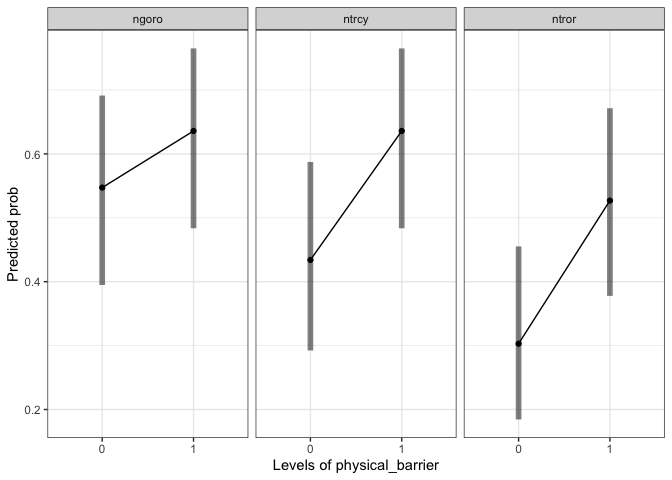
\includegraphics{log-project-aubrie-winnie_files/figure-latex/unnamed-chunk-16-1.pdf}

\begin{Shaded}
\begin{Highlighting}[]
\DocumentationTok{\#\# can test for significance of contribution of the fraction of initial treatment}
\CommentTok{\# do this with partial redundancy analysis}
\CommentTok{\# trt\_Frac\textless{}{-}rda(ass.rel.t012\textasciitilde{} init +Condition(block + time)) \# partial rda model}
\CommentTok{\# summary(trt\_Frac) }
\CommentTok{\# RsquareAdj(trt\_Frac)$adj.r.squared \#explanatory power}
\CommentTok{\# anova.cca(trt\_Frac) \#\# this tells us if first condition, init, significantly contributes to overall variance explanation. }

\DocumentationTok{\#\#\# extracting species scores and plotting }
\CommentTok{\# species scores}
\NormalTok{species.scores}\OtherTok{\textless{}{-}}\FunctionTok{as.data.frame}\NormalTok{(vegan}\SpecialCharTok{::}\FunctionTok{scores}\NormalTok{(ass.rel.t012\_NMS,}\StringTok{"species"}\NormalTok{)) }\DocumentationTok{\#\# some species don\textquotesingle{}t have scores}
\NormalTok{species.scores}\SpecialCharTok{$}\NormalTok{species}\OtherTok{\textless{}{-}}\FunctionTok{rownames}\NormalTok{(species.scores) }

\DocumentationTok{\#\#\# NMDS 1 and 2 }
\NormalTok{log}\OtherTok{\textless{}{-}}\NormalTok{mds\_scores\_t012[mds\_scores\_t012}\SpecialCharTok{$}\NormalTok{treatment }\SpecialCharTok{==} \StringTok{"log"}\NormalTok{, ][}\FunctionTok{chull}\NormalTok{(mds\_scores\_t012[mds\_scores\_t012}\SpecialCharTok{$}\NormalTok{treatment }\SpecialCharTok{==} 
                                                          \StringTok{"log"}\NormalTok{, }\FunctionTok{c}\NormalTok{(}\StringTok{"NMDS1"}\NormalTok{, }\StringTok{"NMDS2"}\NormalTok{)]), ]}

\NormalTok{open}\OtherTok{\textless{}{-}}\NormalTok{mds\_scores\_t012[mds\_scores\_t012}\SpecialCharTok{$}\NormalTok{treatment }\SpecialCharTok{==} \StringTok{"open"}\NormalTok{, ][}\FunctionTok{chull}\NormalTok{(mds\_scores\_t012[mds\_scores\_t012}\SpecialCharTok{$}\NormalTok{treatment }\SpecialCharTok{==} 
                                                               \StringTok{"open"}\NormalTok{, }\FunctionTok{c}\NormalTok{(}\StringTok{"NMDS1"}\NormalTok{, }\StringTok{"NMDS2"}\NormalTok{)]), ]}

\NormalTok{hulldat}\OtherTok{\textless{}{-}}\FunctionTok{rbind}\NormalTok{(log,open)}

\FunctionTok{options}\NormalTok{(}\AttributeTok{ggrepel.max.overlaps =} \ConstantTok{Inf}\NormalTok{)}

\NormalTok{nmds.plot.sp }\OtherTok{\textless{}{-}} \FunctionTok{ggplot}\NormalTok{()}\SpecialCharTok{+}
  \FunctionTok{theme\_bw}\NormalTok{()}\SpecialCharTok{+}
  \FunctionTok{theme}\NormalTok{(}\AttributeTok{panel.background =} \FunctionTok{element\_blank}\NormalTok{(),}
        \AttributeTok{panel.grid.major =} \FunctionTok{element\_blank}\NormalTok{(),  }\CommentTok{\#remove major{-}grid labels}
        \AttributeTok{panel.grid.minor =} \FunctionTok{element\_blank}\NormalTok{(),  }\CommentTok{\#remove minor{-}grid labels}
        \AttributeTok{plot.background =} \FunctionTok{element\_blank}\NormalTok{(), }
        \AttributeTok{axis.text =} \FunctionTok{element\_text}\NormalTok{(}\AttributeTok{size =} \DecValTok{15}\NormalTok{),}
        \AttributeTok{axis.title=}\FunctionTok{element\_text}\NormalTok{(}\AttributeTok{size=}\DecValTok{20}\NormalTok{),}
        \AttributeTok{legend.title=}\FunctionTok{element\_text}\NormalTok{(}\AttributeTok{size=}\DecValTok{20}\NormalTok{), }
        \AttributeTok{legend.text=}\FunctionTok{element\_text}\NormalTok{(}\AttributeTok{size=}\DecValTok{15}\NormalTok{))}\SpecialCharTok{+}
  \FunctionTok{geom\_text\_repel}\NormalTok{(}\AttributeTok{data=}\NormalTok{species.scores, }\FunctionTok{aes}\NormalTok{(NMDS1, NMDS2, }\AttributeTok{label=}\NormalTok{species), }\AttributeTok{alpha=}\FloatTok{0.9}\NormalTok{, }\AttributeTok{size=}\DecValTok{5}\NormalTok{, }\AttributeTok{col=}\StringTok{\textquotesingle{}darkgray\textquotesingle{}}\NormalTok{, }\AttributeTok{na.rm=}\ConstantTok{TRUE}\NormalTok{)}\SpecialCharTok{+}
  \FunctionTok{geom\_polygon}\NormalTok{(}\AttributeTok{data=}\NormalTok{hulldat, }\FunctionTok{aes}\NormalTok{(NMDS1, NMDS2, }\AttributeTok{fill=}\NormalTok{treatment, }\AttributeTok{group=}\NormalTok{treatment), }\AttributeTok{alpha=}\FloatTok{0.3}\NormalTok{)}\SpecialCharTok{+}\FunctionTok{scale\_fill\_manual}\NormalTok{(}\AttributeTok{values=}\FunctionTok{c}\NormalTok{(}\StringTok{"\#63A088"}\NormalTok{,}\StringTok{"\#56638A"}\NormalTok{), }\AttributeTok{name=}\StringTok{"Treatment"}\NormalTok{)}\SpecialCharTok{+}
  \FunctionTok{geom\_point}\NormalTok{(}\AttributeTok{data=}\NormalTok{mds\_scores\_t012, }\FunctionTok{aes}\NormalTok{(NMDS1, NMDS2, }\AttributeTok{shape=}\NormalTok{block, }\AttributeTok{col=}\NormalTok{treatment), }\AttributeTok{size=}\DecValTok{6}\NormalTok{)}\SpecialCharTok{+} \FunctionTok{scale\_shape\_manual}\NormalTok{(}\AttributeTok{values =} \FunctionTok{c}\NormalTok{(}\DecValTok{14}\NormalTok{,}\DecValTok{15}\NormalTok{,}\DecValTok{16}\NormalTok{,}\DecValTok{17}\NormalTok{,}\DecValTok{11}\NormalTok{,}\DecValTok{18}\NormalTok{,}\DecValTok{8}\NormalTok{), }\AttributeTok{name=}\StringTok{\textquotesingle{}Block\textquotesingle{}}\NormalTok{)}\SpecialCharTok{+}
  \FunctionTok{scale\_colour\_manual}\NormalTok{(}\AttributeTok{values=}\FunctionTok{c}\NormalTok{(}\StringTok{"\#63A088"}\NormalTok{,}\StringTok{"\#56638A"}\NormalTok{), }\AttributeTok{name=}\StringTok{"Treatment"}\NormalTok{)}\SpecialCharTok{+}
  \FunctionTok{labs}\NormalTok{(}\AttributeTok{title=}\FunctionTok{paste0}\NormalTok{(}\StringTok{"Stress: "}\NormalTok{, }\FunctionTok{round}\NormalTok{(ass.rel.t012\_NMS}\SpecialCharTok{$}\NormalTok{stress,}\DecValTok{3}\NormalTok{)))}

\NormalTok{nmds.plot.nutrient }\OtherTok{\textless{}{-}} \FunctionTok{ggplot}\NormalTok{()}\SpecialCharTok{+}
  \FunctionTok{theme\_bw}\NormalTok{()}\SpecialCharTok{+}
  \FunctionTok{theme}\NormalTok{(}\AttributeTok{panel.background =} \FunctionTok{element\_blank}\NormalTok{(),}
        \AttributeTok{panel.grid.major =} \FunctionTok{element\_blank}\NormalTok{(),  }\CommentTok{\#remove major{-}grid labels}
        \AttributeTok{panel.grid.minor =} \FunctionTok{element\_blank}\NormalTok{(),  }\CommentTok{\#remove minor{-}grid labels}
        \AttributeTok{plot.background =} \FunctionTok{element\_blank}\NormalTok{(), }
        \AttributeTok{axis.text =} \FunctionTok{element\_text}\NormalTok{(}\AttributeTok{size =} \DecValTok{15}\NormalTok{),}
        \AttributeTok{axis.title=}\FunctionTok{element\_text}\NormalTok{(}\AttributeTok{size=}\DecValTok{20}\NormalTok{),}
        \AttributeTok{legend.title=}\FunctionTok{element\_text}\NormalTok{(}\AttributeTok{size=}\DecValTok{20}\NormalTok{), }
        \AttributeTok{legend.text=}\FunctionTok{element\_text}\NormalTok{(}\AttributeTok{size=}\DecValTok{15}\NormalTok{))}\SpecialCharTok{+}
  \FunctionTok{geom\_polygon}\NormalTok{(}\AttributeTok{data=}\NormalTok{hulldat, }\FunctionTok{aes}\NormalTok{(NMDS1, NMDS2, }\AttributeTok{fill=}\NormalTok{treatment, }\AttributeTok{group=}\NormalTok{treatment),}\AttributeTok{alpha=}\FloatTok{0.3}\NormalTok{)}\SpecialCharTok{+}\FunctionTok{scale\_fill\_manual}\NormalTok{(}\AttributeTok{values=}\FunctionTok{c}\NormalTok{(}\StringTok{"\#63A088"}\NormalTok{,}\StringTok{"\#56638A"}\NormalTok{), }\AttributeTok{name=}\StringTok{"Treatment"}\NormalTok{)}\SpecialCharTok{+}
  \FunctionTok{geom\_point}\NormalTok{(}\AttributeTok{data=}\NormalTok{mds\_scores\_t012, }\FunctionTok{aes}\NormalTok{(NMDS1, NMDS2, }\AttributeTok{shape=}\NormalTok{block, }\AttributeTok{col=}\NormalTok{treatment), }\AttributeTok{size=}\DecValTok{6}\NormalTok{)}\SpecialCharTok{+} \FunctionTok{scale\_shape\_manual}\NormalTok{(}\AttributeTok{values =} \FunctionTok{c}\NormalTok{(}\DecValTok{14}\NormalTok{,}\DecValTok{15}\NormalTok{,}\DecValTok{16}\NormalTok{,}\DecValTok{17}\NormalTok{,}\DecValTok{11}\NormalTok{,}\DecValTok{18}\NormalTok{,}\DecValTok{8}\NormalTok{), }\AttributeTok{name=}\StringTok{\textquotesingle{}Block\textquotesingle{}}\NormalTok{)}\SpecialCharTok{+}
  \FunctionTok{scale\_colour\_manual}\NormalTok{(}\AttributeTok{values=}\FunctionTok{c}\NormalTok{(}\StringTok{"\#63A088"}\NormalTok{,}\StringTok{"\#56638A"}\NormalTok{), }\AttributeTok{name=}\StringTok{"Treatment"}\NormalTok{)}\SpecialCharTok{+}
  \FunctionTok{geom\_segment}\NormalTok{(}\FunctionTok{aes}\NormalTok{(}\AttributeTok{x =} \DecValTok{0}\NormalTok{, }\AttributeTok{y =} \DecValTok{0}\NormalTok{, }\AttributeTok{xend =}\NormalTok{ NMDS1, }\AttributeTok{yend =}\NormalTok{ NMDS2), }
       \AttributeTok{data =}\NormalTok{ en\_coord\_cont, }\AttributeTok{size =}\FloatTok{0.5}\NormalTok{, }\AttributeTok{alpha =} \FloatTok{0.5}\NormalTok{, }\AttributeTok{colour =} \StringTok{"grey30"}\NormalTok{) }\SpecialCharTok{+}
     \FunctionTok{geom\_text}\NormalTok{(}\AttributeTok{data =}\NormalTok{ en\_coord\_cont, }\FunctionTok{aes}\NormalTok{(}\AttributeTok{x =}\NormalTok{ NMDS1, }\AttributeTok{y =}\NormalTok{ NMDS2), }\AttributeTok{colour =} \StringTok{"grey30"}\NormalTok{, }
       \AttributeTok{fontface =} \StringTok{"bold"}\NormalTok{, }\AttributeTok{label =} \FunctionTok{row.names}\NormalTok{(en\_coord\_cont))}\SpecialCharTok{+}
  \FunctionTok{labs}\NormalTok{(}\AttributeTok{title=}\FunctionTok{paste0}\NormalTok{(}\StringTok{"Stress: "}\NormalTok{, }\FunctionTok{round}\NormalTok{(ass.rel.t012\_NMS}\SpecialCharTok{$}\NormalTok{stress,}\DecValTok{3}\NormalTok{)))}
  
\NormalTok{(nmds.plot.sp }\SpecialCharTok{+} \FunctionTok{theme}\NormalTok{(}\AttributeTok{legend.position =} \StringTok{"none"}\NormalTok{)) }\SpecialCharTok{+}\NormalTok{ nmds.plot.nutrient }\SpecialCharTok{+} \FunctionTok{plot\_layout}\NormalTok{(}\AttributeTok{guides =} \StringTok{"collect"}\NormalTok{) }\SpecialCharTok{+} \FunctionTok{plot\_annotation}\NormalTok{(}\AttributeTok{title =} \StringTok{\textquotesingle{}Plant composition: 2020\textquotesingle{}}\NormalTok{)}
\end{Highlighting}
\end{Shaded}

\includegraphics{log-project-aubrie-winnie_files/figure-latex/unnamed-chunk-16-2.pdf}

\hypertarget{interpretation}{%
\paragraph{\texorpdfstring{\emph{Interpretation}}{Interpretation}}\label{interpretation}}

\hypertarget{q3-arehow-are-plant-species-performances-affected-by-proximity-to-fallen-logs}{%
\subsubsection{\texorpdfstring{\textbf{Q3 Are/how are plant species
performances affected by proximity to fallen
logs?}}{Q3 Are/how are plant species performances affected by proximity to fallen logs? }}\label{q3-arehow-are-plant-species-performances-affected-by-proximity-to-fallen-logs}}

\hypertarget{overview-of-results-2}{%
\paragraph{\texorpdfstring{\emph{Overview of results}
}{Overview of results  }}\label{overview-of-results-2}}

\textbf{2021}

There are three response variables: presence (binomial), count
(truncated poisson), and per capita biomass (gaussian).

\emph{Presence} - The best fit model for presence is a tie between
between physical barrier and the additive model of physical barrier +
nutrient island (deltaAIC=0.32). I present the model analysis of the
additive model. - Both TRCY and TROR are significantly more likely to be
present where there is a physical barrier as compared to in the open
(TRCY: p=0.03, TROR: p=0.01) - Nutrient island does not significantly
explain variation in presence/absence in any species. However, all
species trend to having higher probability of presence in log-legacy
plots.

\emph{Count} - The best fit model for count is nutrient island. -
Nutrient island does not strongly significantly explain variation in
presence/absence in any species. TRCY is marginally significantly
affected by nutrient island, where there are more TRCY in plots where
there is a `log legacy' (there had been a decomposing log in the plot
before the experiment began)

\emph{Biomass} - The best fit model for per capita biomass is the
nutrient island, then physical barrier island, then the additive model.
They are all within 2 AICc points of each other (deltaAIC=1.55 and 1.76,
respectively). I present the model analysis of the additive model. -
Nutrient island significantly explains variation GORO biomass, where
there are larger GORO plants in plots where there is a `log legacy'
(p=0.03). - Physical barrier does not explain variation in biomass for
any species.

\textbf{2022}

There are again three response variables: presence (binomial), count
(truncated poisson), and per capita biomass (gaussian).

\emph{Presence} - The best fit model for presence is a tie between
between physical barrier and the additive model of physical barrier +
nutrient island (deltaAIC=0.24). I present the model analysis of the
additive model. - Both TRCY and TROR are significantly more likely to be
present where there is a physical barrier as compared to in the open
(TRCY: p=0.007, TROR: p=0.03) - Nutrient island significantly explains
the presence/absence of TRCY, where TRCY is more likely to be present in
log legacy plots as compared to open legacy plots (p=0.02)

\emph{Count} - The best fit model for count is a tie between nutrient
island and physical barrier. I present the model analysis of the
nutrient island model. - Nutrient island does not strongly significantly
explain variation in presence/absence in any species.

\emph{Biomass} - The best fit model for per capita biomass is the
nutrient island, then the additive model, then the physical barrier
model. They are all within 1 AICc points of each other (deltaAIC=0.31
and 0.46, respectively). I present the model analysis of the additive
model. - Nutrient island significantly explains variation in TROR
biomass, where log legacy plots have larger TROR as compared to open
legacy plots (p=0.04) - Physical barrier significantly explains
variation in TROR biomass, where plots in the open have larger TROR than
plots near a physical barrier (either log or PVC pipe) (p=0.02)

\hypertarget{statistical-methods-2}{%
\paragraph{\texorpdfstring{\emph{Statistical Methods}
}{Statistical Methods  }}\label{statistical-methods-2}}

The basic approach is to analyse count and biomass data from 2021 and
2022 sowing experiment. We sowed 15 seeds for each species into 16 plots
in each of the seven blocks. There are 6 plot type treatments. The gap
and open treatments each have four replicates per block, and the
insitu\_log, insitu\_pvc, open\_with\_log, and open\_with\_pvc each have
two replicates per block. \emph{note: For each treatment of plot type,
there is also a dispersal treatment, but I do not analyse that here
(yet).} - For \textbf{count data} I use a glmmTMB to run a generalized
linear mixed effects model approach to analyse the data. The hurdle
model approach I am using is to first code presence/absence as 0 or 1 (1
being any nonzero count value) and run this analysis as a binomial
regression. Depending on the model fit and residual dispersion (using
DHARMa), I then either run a truncated poisson or truncated negative
binomial regression on the count data. Though I did run alternative
versions of hurdle models that predict count while accounting for zero
inflation, I felt that analyzing the presence/absence, and then
analyzing count, may be revealing more of the biology of the system,
where presence/absence was distinctly affected by treatments while count
was less so. - For \textbf{biomass data} I use linear mixed effects
model to analyse the per capita biomass data. I first do a log(1+n)
transformation on the per capita biomass, then analyze. I chose to do
per capita biomass because of recalcitrant (!!) residual dispersion in
total biomass, even after attemtps at log and square root
transformations. I chose to do a model selection approach, which I'm
trying to move away from generally. However, the models I use to analyze
the data represent different hypotheses about \emph{why} plant species
might perform differently, and so I chose to do a model comparison and
selection approach as a way to not only understand how plant species
performance is affected by proximity to fallen logs, but also gain
insight as to why this may be the case.

N.B.:Model comparison might not be the approach we want, and we may want
to run the analysis differently. I'm open to discussion and change on
this point.

After model comparison, I use estimated marginal means (package emmeans)
on the best fit model and compute the significance of the difference in
estimates.

The models I use test the hypotheses from above: Log decomposition
creates islands of fertility directly around the fallen log and fallen
logs alter the microclimate directly around them by providing shade.

\hypertarget{analysis-2}{%
\paragraph{\texorpdfstring{\emph{Analysis}}{Analysis }}\label{analysis-2}}

\hypertarget{section}{%
\subparagraph{\texorpdfstring{\textbf{2021}}{2021}}\label{section}}

\begin{Shaded}
\begin{Highlighting}[]
\DocumentationTok{\#\#\# doing vital rate analysis}

\CommentTok{\# packages }
\FunctionTok{require}\NormalTok{(lme4)}
\FunctionTok{require}\NormalTok{(emmeans)}
\FunctionTok{require}\NormalTok{(pscl)}
\FunctionTok{require}\NormalTok{(glmmTMB)}
\FunctionTok{require}\NormalTok{(tidyr)}
\FunctionTok{require}\NormalTok{(DHARMa)}
\FunctionTok{require}\NormalTok{(ggplot2)}
\FunctionTok{require}\NormalTok{(AICcmodavg)}
\FunctionTok{require}\NormalTok{(ggpubr)}

\DocumentationTok{\#\#\#\#\#\#\#\#\#\#\#\#\#\# 2021 data \#\#\#\#\#\#\#\#\#\#\#\#\#}

\CommentTok{\# read csv}
\NormalTok{dat}\OtherTok{\textless{}{-}}\FunctionTok{read.csv}\NormalTok{(}\StringTok{\textquotesingle{}nplants\_data\_2021\_git.csv\textquotesingle{}}\NormalTok{, }\AttributeTok{header=}\NormalTok{T)}
\NormalTok{dat1}\OtherTok{\textless{}{-}}\NormalTok{dat[}\FunctionTok{which}\NormalTok{(dat}\SpecialCharTok{$}\NormalTok{seeding\_trt}\SpecialCharTok{==}\DecValTok{1}\NormalTok{),]}
\NormalTok{dat1}\SpecialCharTok{$}\NormalTok{physical\_barrier}\OtherTok{\textless{}{-}}\FunctionTok{as.factor}\NormalTok{(dat1}\SpecialCharTok{$}\NormalTok{physical\_barrier)}
\NormalTok{dat1}\SpecialCharTok{$}\NormalTok{block}\OtherTok{\textless{}{-}}\FunctionTok{as.factor}\NormalTok{(dat1}\SpecialCharTok{$}\NormalTok{block)}

\DocumentationTok{\#\#\#\#\#\#\#\#\#\#\#\#\# treatment response: do analysis for count by species \#\#\#\#\#\#\#\#\#\#\#\#\# }

\NormalTok{dat2}\OtherTok{\textless{}{-}}\NormalTok{(dat1[}\FunctionTok{c}\NormalTok{(}\DecValTok{1}\SpecialCharTok{:}\DecValTok{4}\NormalTok{,}\DecValTok{7}\NormalTok{,}\DecValTok{11}\NormalTok{,}\DecValTok{15}\NormalTok{,}\DecValTok{22}\NormalTok{)]) }\CommentTok{\# these are block, transect, initial, current\_plot\_type, ngoro, ntrcy, ntror, physical\_barrier}
\FunctionTok{head}\NormalTok{(dat2) }
\end{Highlighting}
\end{Shaded}

\begin{verbatim}
##   block transect initial current_plot_type ngoro ntrcy ntror physical_barrier
## 1     1     1.01     log               gap     3     0     0                0
## 2     1     1.02     log        insitu_log     0     0     0                1
## 3     1     1.03     log        insitu_pvc     1     3     3                1
## 4     1     1.14     log        insitu_log     0     0     0                1
## 5     1     1.17    open              open     0     0     0                0
## 6     1     1.19    open              open     2     0     0                0
\end{verbatim}

\begin{Shaded}
\begin{Highlighting}[]
\NormalTok{countdat}\OtherTok{\textless{}{-}}\FunctionTok{as.data.frame}\NormalTok{(dat2 }\SpecialCharTok{\%\textgreater{}\%} \FunctionTok{pivot\_longer}\NormalTok{(}\FunctionTok{c}\NormalTok{(ntror, ngoro, ntrcy)))}
\NormalTok{countdat}\SpecialCharTok{$}\NormalTok{value}\OtherTok{\textless{}{-}}\FunctionTok{as.numeric}\NormalTok{(}\FunctionTok{ifelse}\NormalTok{(countdat}\SpecialCharTok{$}\NormalTok{value}\SpecialCharTok{\textgreater{}}\DecValTok{15}\NormalTok{, }\DecValTok{15}\NormalTok{, countdat}\SpecialCharTok{$}\NormalTok{value))}
\NormalTok{countmod}\OtherTok{\textless{}{-}}\FunctionTok{glmmTMB}\NormalTok{(value}\SpecialCharTok{\textasciitilde{}}\NormalTok{name}\SpecialCharTok{*}\NormalTok{current\_plot\_type}\SpecialCharTok{+}\NormalTok{(}\DecValTok{1}\SpecialCharTok{|}\NormalTok{block), }\AttributeTok{family=}\StringTok{"poisson"}\NormalTok{, }\AttributeTok{data=}\NormalTok{countdat)}

\CommentTok{\# test for fit and zero inflation}
\NormalTok{ sim}\OtherTok{\textless{}{-}}\FunctionTok{simulateResiduals}\NormalTok{(countmod)}
 \FunctionTok{testZeroInflation}\NormalTok{(sim) }\CommentTok{\# zero{-}inflated so need something else }
\end{Highlighting}
\end{Shaded}

\includegraphics{log-project-aubrie-winnie_files/figure-latex/2021 growth-1.pdf}

\begin{verbatim}
## 
##  DHARMa zero-inflation test via comparison to expected zeros with
##  simulation under H0 = fitted model
## 
## data:  simulationOutput
## ratioObsSim = 1.5731, p-value < 2.2e-16
## alternative hypothesis: two.sided
\end{verbatim}

\begin{Shaded}
\begin{Highlighting}[]
 \FunctionTok{plot}\NormalTok{(sim)}
\end{Highlighting}
\end{Shaded}

\includegraphics{log-project-aubrie-winnie_files/figure-latex/2021 growth-2.pdf}

\begin{Shaded}
\begin{Highlighting}[]
\DocumentationTok{\#\# going to do a hurdle model, which assumes a zero is only generated in one way }
\CommentTok{\# https://jsdajournal.springeropen.com/articles/10.1186/s40488{-}021{-}00121{-}4}
\CommentTok{\# \#https://stats.stackexchange.com/questions/81457/what{-}is{-}the{-}difference{-}between{-}zero{-}inflated{-}and{-}hurdle{-}models}

\CommentTok{\# hurdle model }
\CommentTok{\# using examples as presented here: https://www.biorxiv.org/content/biorxiv/suppl/2017/05/01/132753.DC1/132753{-}2.pdf }
\NormalTok{fit3}\OtherTok{\textless{}{-}}\FunctionTok{glmmTMB}\NormalTok{(value}\SpecialCharTok{\textasciitilde{}}\NormalTok{name}\SpecialCharTok{*}\NormalTok{current\_plot\_type}\SpecialCharTok{+}\NormalTok{(}\DecValTok{1}\SpecialCharTok{|}\NormalTok{block), }\AttributeTok{ziformula=}\SpecialCharTok{\textasciitilde{}}\NormalTok{., }\AttributeTok{family=}\FunctionTok{nbinom2}\NormalTok{(), }\AttributeTok{data=}\NormalTok{countdat)}
\NormalTok{ sim3}\OtherTok{\textless{}{-}}\FunctionTok{simulateResiduals}\NormalTok{(fit3)}
 \FunctionTok{plot}\NormalTok{(sim3)}
\end{Highlighting}
\end{Shaded}

\includegraphics{log-project-aubrie-winnie_files/figure-latex/2021 growth-3.pdf}

\begin{Shaded}
\begin{Highlighting}[]
 \FunctionTok{testDispersion}\NormalTok{(sim3) }\CommentTok{\# looks nice ! }
\end{Highlighting}
\end{Shaded}

\includegraphics{log-project-aubrie-winnie_files/figure-latex/2021 growth-4.pdf}

\begin{verbatim}
## 
##  DHARMa nonparametric dispersion test via sd of residuals fitted vs.
##  simulated
## 
## data:  simulationOutput
## dispersion = 0.99071, p-value = 0.896
## alternative hypothesis: two.sided
\end{verbatim}

\begin{Shaded}
\begin{Highlighting}[]
 \FunctionTok{testZeroInflation}\NormalTok{(sim3) }\CommentTok{\# looks nice ! }
\end{Highlighting}
\end{Shaded}

\includegraphics{log-project-aubrie-winnie_files/figure-latex/2021 growth-5.pdf}

\begin{verbatim}
## 
##  DHARMa zero-inflation test via comparison to expected zeros with
##  simulation under H0 = fitted model
## 
## data:  simulationOutput
## ratioObsSim = 0.99276, p-value = 0.912
## alternative hypothesis: two.sided
\end{verbatim}

\begin{Shaded}
\begin{Highlighting}[]
\FunctionTok{summary}\NormalTok{(fit3)}
\end{Highlighting}
\end{Shaded}

\begin{verbatim}
##  Family: nbinom2  ( log )
## Formula:          value ~ name * current_plot_type + (1 | block)
## Zero inflation:         ~.
## Data: countdat
## 
##      AIC      BIC   logLik deviance df.resid 
##   1101.2   1250.1   -511.6   1023.2      297 
## 
## Random effects:
## 
## Conditional model:
##  Groups Name        Variance Std.Dev.
##  block  (Intercept) 0.03237  0.1799  
## Number of obs: 336, groups:  block, 7
## 
## Zero-inflation model:
##  Groups Name        Variance Std.Dev.
##  block  (Intercept) 0.9243   0.9614  
## Number of obs: 336, groups:  block, 7
## 
## Dispersion parameter for nbinom2 family (): 1.68 
## 
## Conditional model:
##                                          Estimate Std. Error z value Pr(>|z|)  
## (Intercept)                               0.42749    0.31299   1.366   0.1720  
## namentrcy                                 0.82532    0.39283   2.101   0.0356 *
## namentror                                -0.12276    0.44057  -0.279   0.7805  
## current_plot_typeinsitu_log              -1.07022    0.53312  -2.007   0.0447 *
## current_plot_typeinsitu_pvc              -0.02408    0.44823  -0.054   0.9572  
## current_plot_typeopen                    -0.05040    0.40107  -0.126   0.9000  
## current_plot_typeopen_with_log           -0.24213    0.50393  -0.480   0.6309  
## current_plot_typeopen_with_pvc            0.35404    0.40916   0.865   0.3869  
## namentrcy:current_plot_typeinsitu_log     1.05024    0.67754   1.550   0.1211  
## namentror:current_plot_typeinsitu_log     0.83983    0.81808   1.027   0.3046  
## namentrcy:current_plot_typeinsitu_pvc    -0.20308    0.59085  -0.344   0.7311  
## namentror:current_plot_typeinsitu_pvc     0.61733    0.63892   0.966   0.3339  
## namentrcy:current_plot_typeopen          -0.51151    0.60272  -0.849   0.3961  
## namentror:current_plot_typeopen           0.50564    0.70479   0.717   0.4731  
## namentrcy:current_plot_typeopen_with_log -0.05338    0.70024  -0.076   0.9392  
## namentror:current_plot_typeopen_with_log  0.31312    0.75666   0.414   0.6790  
## namentrcy:current_plot_typeopen_with_pvc -1.04638    0.57985  -1.805   0.0711 .
## namentror:current_plot_typeopen_with_pvc -0.33034    0.59667  -0.554   0.5798  
## ---
## Signif. codes:  0 '***' 0.001 '**' 0.01 '*' 0.05 '.' 0.1 ' ' 1
## 
## Zero-inflation model:
##                                            Estimate Std. Error z value Pr(>|z|)
## (Intercept)                              -1.396e+00  1.135e+00  -1.230    0.219
## namentrcy                                 9.858e-01  1.131e+00   0.872    0.383
## namentror                                 4.034e-01  1.305e+00   0.309    0.757
## current_plot_typeinsitu_log              -1.628e+01  5.111e+03  -0.003    0.997
## current_plot_typeinsitu_pvc              -2.684e+00  7.986e+00  -0.336    0.737
## current_plot_typeopen                    -1.280e+00  2.202e+00  -0.582    0.561
## current_plot_typeopen_with_log           -9.202e-01  2.380e+00  -0.387    0.699
## current_plot_typeopen_with_pvc           -1.790e+01  4.876e+03  -0.004    0.997
## namentrcy:current_plot_typeinsitu_log     1.551e+01  5.111e+03   0.003    0.998
## namentror:current_plot_typeinsitu_log     1.661e+01  5.111e+03   0.003    0.997
## namentrcy:current_plot_typeinsitu_pvc    -5.449e-01  8.249e+00  -0.066    0.947
## namentror:current_plot_typeinsitu_pvc     1.947e+00  8.039e+00   0.242    0.809
## namentrcy:current_plot_typeopen           1.665e+00  2.423e+00   0.687    0.492
## namentror:current_plot_typeopen           3.564e+00  2.581e+00   1.381    0.167
## namentrcy:current_plot_typeopen_with_log  5.747e-01  2.630e+00   0.218    0.827
## namentror:current_plot_typeopen_with_log  8.341e-01  2.920e+00   0.286    0.775
## namentrcy:current_plot_typeopen_with_pvc  1.553e+01  4.876e+03   0.003    0.997
## namentror:current_plot_typeopen_with_pvc -9.760e+00  5.916e+05   0.000    1.000
\end{verbatim}

\begin{Shaded}
\begin{Highlighting}[]
\FunctionTok{emmip}\NormalTok{(fit3,}\SpecialCharTok{\textasciitilde{}}\NormalTok{current\_plot\_type}\SpecialCharTok{|}\NormalTok{name, }\AttributeTok{type=}\StringTok{\textquotesingle{}response\textquotesingle{}}\NormalTok{,}\AttributeTok{CI=}\NormalTok{T)}
\end{Highlighting}
\end{Shaded}

\includegraphics{log-project-aubrie-winnie_files/figure-latex/2021 growth-6.pdf}

\begin{Shaded}
\begin{Highlighting}[]
\CommentTok{\# visualize}
\NormalTok{est}\OtherTok{\textless{}{-}}\FunctionTok{emmeans}\NormalTok{(fit3,}\SpecialCharTok{\textasciitilde{}}\NormalTok{current\_plot\_type}\SpecialCharTok{|}\NormalTok{name, }\AttributeTok{type=}\StringTok{\textquotesingle{}response\textquotesingle{}}\NormalTok{)}
\FunctionTok{pairs}\NormalTok{(est)}
\end{Highlighting}
\end{Shaded}

\begin{verbatim}
## name = ngoro:
##  contrast                      ratio    SE  df null z.ratio p.value
##  gap / insitu_log              2.916 1.555 Inf    1   2.007  0.3379
##  gap / insitu_pvc              1.024 0.459 Inf    1   0.054  1.0000
##  gap / open                    1.052 0.422 Inf    1   0.126  1.0000
##  gap / open_with_log           1.274 0.642 Inf    1   0.480  0.9968
##  gap / open_with_pvc           0.702 0.287 Inf    1  -0.865  0.9547
##  insitu_log / insitu_pvc       0.351 0.198 Inf    1  -1.855  0.4301
##  insitu_log / open             0.361 0.189 Inf    1  -1.943  0.3759
##  insitu_log / open_with_log    0.437 0.261 Inf    1  -1.385  0.7365
##  insitu_log / open_with_pvc    0.241 0.123 Inf    1  -2.777  0.0611
##  insitu_pvc / open             1.027 0.443 Inf    1   0.061  1.0000
##  insitu_pvc / open_with_log    1.244 0.667 Inf    1   0.407  0.9986
##  insitu_pvc / open_with_pvc    0.685 0.308 Inf    1  -0.842  0.9596
##  open / open_with_log          1.211 0.588 Inf    1   0.395  0.9988
##  open / open_with_pvc          0.667 0.266 Inf    1  -1.015  0.9131
##  open_with_log / open_with_pvc 0.551 0.270 Inf    1  -1.215  0.8297
## 
## name = ntrcy:
##  contrast                      ratio    SE  df null z.ratio p.value
##  gap / insitu_log              1.020 0.442 Inf    1   0.046  1.0000
##  gap / insitu_pvc              1.255 0.483 Inf    1   0.590  0.9917
##  gap / open                    1.754 0.770 Inf    1   1.280  0.7961
##  gap / open_with_log           1.344 0.642 Inf    1   0.619  0.9897
##  gap / open_with_pvc           1.998 0.840 Inf    1   1.648  0.5668
##  insitu_log / insitu_pvc       1.230 0.545 Inf    1   0.467  0.9972
##  insitu_log / open             1.719 0.827 Inf    1   1.127  0.8704
##  insitu_log / open_with_log    1.317 0.721 Inf    1   0.503  0.9961
##  insitu_log / open_with_pvc    1.959 0.928 Inf    1   1.420  0.7149
##  insitu_pvc / open             1.398 0.619 Inf    1   0.756  0.9747
##  insitu_pvc / open_with_log    1.071 0.531 Inf    1   0.138  1.0000
##  insitu_pvc / open_with_pvc    1.592 0.684 Inf    1   1.083  0.8885
##  open / open_with_log          0.766 0.421 Inf    1  -0.485  0.9967
##  open / open_with_pvc          1.139 0.543 Inf    1   0.273  0.9998
##  open_with_log / open_with_pvc 1.487 0.784 Inf    1   0.752  0.9752
## 
## name = ntror:
##  contrast                      ratio    SE  df null z.ratio p.value
##  gap / insitu_log              1.259 0.788 Inf    1   0.368  0.9991
##  gap / insitu_pvc              0.553 0.255 Inf    1  -1.283  0.7944
##  gap / open                    0.634 0.369 Inf    1  -0.783  0.9704
##  gap / open_with_log           0.931 0.520 Inf    1  -0.127  1.0000
##  gap / open_with_pvc           0.977 0.441 Inf    1  -0.053  1.0000
##  insitu_log / insitu_pvc       0.439 0.274 Inf    1  -1.321  0.7735
##  insitu_log / open             0.504 0.362 Inf    1  -0.954  0.9323
##  insitu_log / open_with_log    0.740 0.520 Inf    1  -0.429  0.9982
##  insitu_log / open_with_pvc    0.776 0.477 Inf    1  -0.413  0.9985
##  insitu_pvc / open             1.148 0.666 Inf    1   0.238  0.9999
##  insitu_pvc / open_with_log    1.686 0.948 Inf    1   0.929  0.9392
##  insitu_pvc / open_with_pvc    1.767 0.780 Inf    1   1.291  0.7900
##  open / open_with_log          1.469 0.975 Inf    1   0.579  0.9924
##  open / open_with_pvc          1.540 0.882 Inf    1   0.753  0.9751
##  open_with_log / open_with_pvc 1.048 0.575 Inf    1   0.086  1.0000
## 
## P value adjustment: tukey method for comparing a family of 6 estimates 
## Tests are performed on the log scale
\end{verbatim}

\begin{Shaded}
\begin{Highlighting}[]
\DocumentationTok{\#\#\#\# now i\textquotesingle{}ll do a by{-}hand hurdle model on my own using a truncated negative binomial}

\DocumentationTok{\#\#\# zeros and ones }
\NormalTok{countdat}\SpecialCharTok{$}\NormalTok{presence}\OtherTok{\textless{}{-}}\FunctionTok{ifelse}\NormalTok{(countdat}\SpecialCharTok{$}\NormalTok{value}\SpecialCharTok{==}\DecValTok{0}\NormalTok{, }\DecValTok{0}\NormalTok{, }\DecValTok{1}\NormalTok{)}
\NormalTok{zerofit}\OtherTok{\textless{}{-}}\FunctionTok{glmmTMB}\NormalTok{(presence}\SpecialCharTok{\textasciitilde{}}\NormalTok{name}\SpecialCharTok{*}\NormalTok{current\_plot\_type}\SpecialCharTok{+}\NormalTok{(}\DecValTok{1} \SpecialCharTok{|}\NormalTok{ block), }\AttributeTok{family=}\NormalTok{binomial, }\AttributeTok{data=}\NormalTok{countdat, }\AttributeTok{REML=}\ConstantTok{FALSE}\NormalTok{)}
\FunctionTok{emmip}\NormalTok{(zerofit,}\SpecialCharTok{\textasciitilde{}}\NormalTok{current\_plot\_type}\SpecialCharTok{|}\NormalTok{name, }\AttributeTok{type=}\StringTok{\textquotesingle{}response\textquotesingle{}}\NormalTok{,}\AttributeTok{CI=}\NormalTok{T)}
\end{Highlighting}
\end{Shaded}

\includegraphics{log-project-aubrie-winnie_files/figure-latex/2021 growth-7.pdf}

\begin{Shaded}
\begin{Highlighting}[]
\NormalTok{est}\OtherTok{\textless{}{-}}\FunctionTok{emmeans}\NormalTok{(zerofit, }\SpecialCharTok{\textasciitilde{}}\NormalTok{current\_plot\_type}\SpecialCharTok{|}\NormalTok{name, }\AttributeTok{type=}\StringTok{\textquotesingle{}response\textquotesingle{}}\NormalTok{)}
\FunctionTok{pairs}\NormalTok{(est)}
\end{Highlighting}
\end{Shaded}

\begin{verbatim}
## name = ngoro:
##  contrast                      odds.ratio    SE  df null z.ratio p.value
##  gap / insitu_log                   1.175 0.808 Inf    1   0.235  0.9999
##  gap / insitu_pvc                   0.656 0.434 Inf    1  -0.638  0.9882
##  gap / open                         0.676 0.376 Inf    1  -0.705  0.9814
##  gap / open_with_log                0.741 0.499 Inf    1  -0.446  0.9978
##  gap / open_with_pvc                0.145 0.125 Inf    1  -2.246  0.2167
##  insitu_log / insitu_pvc            0.558 0.437 Inf    1  -0.745  0.9763
##  insitu_log / open                  0.575 0.400 Inf    1  -0.796  0.9684
##  insitu_log / open_with_log         0.630 0.500 Inf    1  -0.582  0.9922
##  insitu_log / open_with_pvc         0.123 0.118 Inf    1  -2.189  0.2430
##  insitu_pvc / open                  1.030 0.690 Inf    1   0.045  1.0000
##  insitu_pvc / open_with_log         1.130 0.870 Inf    1   0.159  1.0000
##  insitu_pvc / open_with_pvc         0.221 0.207 Inf    1  -1.610  0.5920
##  open / open_with_log               1.097 0.747 Inf    1   0.135  1.0000
##  open / open_with_pvc               0.215 0.186 Inf    1  -1.777  0.4805
##  open_with_log / open_with_pvc      0.196 0.185 Inf    1  -1.725  0.5148
## 
## name = ntrcy:
##  contrast                      odds.ratio    SE  df null z.ratio p.value
##  gap / insitu_log                   0.612 0.428 Inf    1  -0.702  0.9818
##  gap / insitu_pvc                   0.350 0.248 Inf    1  -1.483  0.6755
##  gap / open                         1.737 0.974 Inf    1   0.984  0.9231
##  gap / open_with_log                1.000 0.668 Inf    1   0.000  1.0000
##  gap / open_with_pvc                0.487 0.331 Inf    1  -1.059  0.8976
##  insitu_log / insitu_pvc            0.571 0.475 Inf    1  -0.673  0.9849
##  insitu_log / open                  2.837 2.017 Inf    1   1.467  0.6857
##  insitu_log / open_with_log         1.633 1.304 Inf    1   0.614  0.9900
##  insitu_log / open_with_pvc         0.796 0.642 Inf    1  -0.283  0.9998
##  insitu_pvc / open                  4.965 3.577 Inf    1   2.224  0.2265
##  insitu_pvc / open_with_log         2.858 2.306 Inf    1   1.302  0.7842
##  insitu_pvc / open_with_pvc         1.393 1.135 Inf    1   0.407  0.9986
##  open / open_with_log               0.576 0.392 Inf    1  -0.811  0.9656
##  open / open_with_pvc               0.281 0.194 Inf    1  -1.838  0.4411
##  open_with_log / open_with_pvc      0.487 0.381 Inf    1  -0.920  0.9415
## 
## name = ntror:
##  contrast                      odds.ratio    SE  df null z.ratio p.value
##  gap / insitu_log                   1.211 0.848 Inf    1   0.273  0.9998
##  gap / insitu_pvc                   0.360 0.245 Inf    1  -1.499  0.6651
##  gap / open                         3.440 2.188 Inf    1   1.942  0.3763
##  gap / open_with_log                1.000 0.675 Inf    1   0.000  1.0000
##  gap / open_with_pvc                0.487 0.323 Inf    1  -1.083  0.8882
##  insitu_log / insitu_pvc            0.298 0.240 Inf    1  -1.501  0.6637
##  insitu_log / open                  2.841 2.185 Inf    1   1.358  0.7523
##  insitu_log / open_with_log         0.826 0.662 Inf    1  -0.238  0.9999
##  insitu_log / open_with_pvc         0.402 0.319 Inf    1  -1.149  0.8608
##  insitu_pvc / open                  9.545 7.181 Inf    1   2.999  0.0324
##  insitu_pvc / open_with_log         2.775 2.178 Inf    1   1.301  0.7848
##  insitu_pvc / open_with_pvc         1.351 1.047 Inf    1   0.388  0.9989
##  open / open_with_log               0.291 0.217 Inf    1  -1.656  0.5612
##  open / open_with_pvc               0.142 0.104 Inf    1  -2.652  0.0851
##  open_with_log / open_with_pvc      0.487 0.375 Inf    1  -0.934  0.9377
## 
## P value adjustment: tukey method for comparing a family of 6 estimates 
## Tests are performed on the log odds ratio scale
\end{verbatim}

\begin{Shaded}
\begin{Highlighting}[]
\DocumentationTok{\#\#\# abundance with a truncated negbinom }
\NormalTok{countdat}\SpecialCharTok{$}\NormalTok{posicounts}\OtherTok{\textless{}{-}}\FunctionTok{as.numeric}\NormalTok{(}\FunctionTok{ifelse}\NormalTok{(countdat}\SpecialCharTok{$}\NormalTok{value}\SpecialCharTok{==}\DecValTok{0}\NormalTok{, }\StringTok{"NA"}\NormalTok{, countdat}\SpecialCharTok{$}\NormalTok{value))}
\NormalTok{countfit}\OtherTok{\textless{}{-}}\FunctionTok{glmmTMB}\NormalTok{(posicounts}\SpecialCharTok{\textasciitilde{}}\NormalTok{name}\SpecialCharTok{*}\NormalTok{current\_plot\_type}\SpecialCharTok{+}\NormalTok{(}\DecValTok{1} \SpecialCharTok{|}\NormalTok{ block), }\AttributeTok{family=}\FunctionTok{truncated\_nbinom2}\NormalTok{(), }\AttributeTok{data=}\NormalTok{countdat, }\AttributeTok{REML=}\ConstantTok{FALSE}\NormalTok{)}
\FunctionTok{emmip}\NormalTok{(countfit,}\SpecialCharTok{\textasciitilde{}}\NormalTok{current\_plot\_type}\SpecialCharTok{|}\NormalTok{name, }\AttributeTok{type=}\StringTok{\textquotesingle{}response\textquotesingle{}}\NormalTok{,}\AttributeTok{CI=}\NormalTok{T)}
\end{Highlighting}
\end{Shaded}

\includegraphics{log-project-aubrie-winnie_files/figure-latex/2021 growth-8.pdf}

\begin{Shaded}
\begin{Highlighting}[]
\NormalTok{est}\OtherTok{\textless{}{-}}\FunctionTok{emmeans}\NormalTok{(countfit, }\SpecialCharTok{\textasciitilde{}}\NormalTok{current\_plot\_type}\SpecialCharTok{|}\NormalTok{name, }\AttributeTok{type=}\StringTok{\textquotesingle{}response\textquotesingle{}}\NormalTok{)}
\FunctionTok{pairs}\NormalTok{(est)}
\end{Highlighting}
\end{Shaded}

\begin{verbatim}
## name = ngoro:
##  contrast                      ratio    SE  df null z.ratio p.value
##  gap / insitu_log              8.005 8.954 Inf    1   1.860  0.4273
##  gap / insitu_pvc              0.936 0.491 Inf    1  -0.126  1.0000
##  gap / open                    1.074 0.491 Inf    1   0.155  1.0000
##  gap / open_with_log           1.545 0.919 Inf    1   0.731  0.9781
##  gap / open_with_pvc           0.928 0.442 Inf    1  -0.157  1.0000
##  insitu_log / insitu_pvc       0.117 0.134 Inf    1  -1.877  0.4162
##  insitu_log / open             0.134 0.149 Inf    1  -1.804  0.4634
##  insitu_log / open_with_log    0.193 0.227 Inf    1  -1.399  0.7276
##  insitu_log / open_with_pvc    0.116 0.130 Inf    1  -1.923  0.3880
##  insitu_pvc / open             1.147 0.591 Inf    1   0.266  0.9998
##  insitu_pvc / open_with_log    1.650 1.056 Inf    1   0.783  0.9705
##  insitu_pvc / open_with_pvc    0.992 0.528 Inf    1  -0.016  1.0000
##  open / open_with_log          1.439 0.844 Inf    1   0.620  0.9896
##  open / open_with_pvc          0.864 0.403 Inf    1  -0.313  0.9996
##  open_with_log / open_with_pvc 0.601 0.360 Inf    1  -0.849  0.9582
## 
## name = ntrcy:
##  contrast                      ratio    SE  df null z.ratio p.value
##  gap / insitu_log              1.029 0.484 Inf    1   0.061  1.0000
##  gap / insitu_pvc              1.144 0.497 Inf    1   0.310  0.9996
##  gap / open                    1.790 0.845 Inf    1   1.233  0.8207
##  gap / open_with_log           1.246 0.628 Inf    1   0.437  0.9980
##  gap / open_with_pvc           2.168 1.045 Inf    1   1.605  0.5953
##  insitu_log / insitu_pvc       1.112 0.549 Inf    1   0.214  0.9999
##  insitu_log / open             1.739 0.913 Inf    1   1.055  0.8991
##  insitu_log / open_with_log    1.211 0.685 Inf    1   0.339  0.9994
##  insitu_log / open_with_pvc    2.107 1.144 Inf    1   1.372  0.7437
##  insitu_pvc / open             1.565 0.768 Inf    1   0.912  0.9436
##  insitu_pvc / open_with_log    1.089 0.579 Inf    1   0.161  1.0000
##  insitu_pvc / open_with_pvc    1.895 0.965 Inf    1   1.255  0.8094
##  open / open_with_log          0.696 0.394 Inf    1  -0.639  0.9881
##  open / open_with_pvc          1.211 0.656 Inf    1   0.354  0.9993
##  open_with_log / open_with_pvc 1.739 0.992 Inf    1   0.970  0.9274
## 
## name = ntror:
##  contrast                      ratio    SE  df null z.ratio p.value
##  gap / insitu_log              1.536 1.136 Inf    1   0.580  0.9923
##  gap / insitu_pvc              0.622 0.320 Inf    1  -0.924  0.9406
##  gap / open                    0.618 0.388 Inf    1  -0.766  0.9731
##  gap / open_with_log           0.843 0.519 Inf    1  -0.277  0.9998
##  gap / open_with_pvc           0.935 0.520 Inf    1  -0.122  1.0000
##  insitu_log / insitu_pvc       0.405 0.299 Inf    1  -1.225  0.8246
##  insitu_log / open             0.402 0.330 Inf    1  -1.110  0.8774
##  insitu_log / open_with_log    0.549 0.446 Inf    1  -0.737  0.9773
##  insitu_log / open_with_pvc    0.608 0.468 Inf    1  -0.646  0.9874
##  insitu_pvc / open             0.994 0.620 Inf    1  -0.009  1.0000
##  insitu_pvc / open_with_log    1.356 0.833 Inf    1   0.497  0.9963
##  insitu_pvc / open_with_pvc    1.503 0.829 Inf    1   0.739  0.9770
##  open / open_with_log          1.364 0.973 Inf    1   0.436  0.9980
##  open / open_with_pvc          1.512 0.999 Inf    1   0.626  0.9891
##  open_with_log / open_with_pvc 1.108 0.717 Inf    1   0.159  1.0000
## 
## P value adjustment: tukey method for comparing a family of 6 estimates 
## Tests are performed on the log scale
\end{verbatim}

\begin{Shaded}
\begin{Highlighting}[]
\DocumentationTok{\#\#\#\#\#\#\#\#\#\#\#\#\# treatment response: do analysis for total biomass by species \#\#\#\#\#\#\#\#\#\#\#\#\#}

\NormalTok{dat3}\OtherTok{\textless{}{-}}\NormalTok{(dat1[}\FunctionTok{c}\NormalTok{(}\DecValTok{1}\SpecialCharTok{:}\DecValTok{4}\NormalTok{,}\DecValTok{10}\NormalTok{,}\DecValTok{14}\NormalTok{,}\DecValTok{18}\NormalTok{,}\DecValTok{22}\NormalTok{)])}
\NormalTok{totwtdat}\OtherTok{\textless{}{-}}\FunctionTok{as.data.frame}\NormalTok{(dat3 }\SpecialCharTok{\%\textgreater{}\%} \FunctionTok{pivot\_longer}\NormalTok{(}\FunctionTok{c}\NormalTok{(wt\_max15\_goro, wt\_max15\_tror, wt\_max15\_trcy)))}
\NormalTok{totwtdat}\SpecialCharTok{$}\NormalTok{log\_wt}\OtherTok{\textless{}{-}}\FunctionTok{log}\NormalTok{(totwtdat}\SpecialCharTok{$}\NormalTok{value) }\CommentTok{\# log transform the weight data to get it normal looking}

\CommentTok{\# model}
\NormalTok{totwtmod}\OtherTok{\textless{}{-}}\FunctionTok{lmer}\NormalTok{(log\_wt}\SpecialCharTok{\textasciitilde{}}\NormalTok{name}\SpecialCharTok{*}\NormalTok{current\_plot\_type}\SpecialCharTok{+}\NormalTok{(}\DecValTok{1}\SpecialCharTok{|}\NormalTok{block), }\AttributeTok{data=}\NormalTok{totwtdat, }\AttributeTok{REML=}\ConstantTok{FALSE}\NormalTok{)}

\CommentTok{\# test for fit, looks pretty good}
\NormalTok{sim}\OtherTok{\textless{}{-}}\FunctionTok{simulateResiduals}\NormalTok{(totwtmod)}
\FunctionTok{plot}\NormalTok{(sim)}
\end{Highlighting}
\end{Shaded}

\includegraphics{log-project-aubrie-winnie_files/figure-latex/2021 growth-9.pdf}

\begin{Shaded}
\begin{Highlighting}[]
\CommentTok{\# model summary}
\FunctionTok{summary}\NormalTok{(totwtmod)}
\end{Highlighting}
\end{Shaded}

\begin{verbatim}
## Linear mixed model fit by maximum likelihood . t-tests use Satterthwaite's
##   method [lmerModLmerTest]
## Formula: log_wt ~ name * current_plot_type + (1 | block)
##    Data: totwtdat
## 
##      AIC      BIC   logLik deviance df.resid 
##    586.5    649.6   -273.2    546.5      153 
## 
## Scaled residuals: 
##     Min      1Q  Median      3Q     Max 
## -2.3315 -0.7238  0.1635  0.6845  2.3280 
## 
## Random effects:
##  Groups   Name        Variance Std.Dev.
##  block    (Intercept) 0.04225  0.2055  
##  Residual             1.34718  1.1607  
## Number of obs: 173, groups:  block, 7
## 
## Fixed effects:
##                                                    Estimate Std. Error
## (Intercept)                                       -2.143222   0.320185
## namewt_max15_trcy                                 -0.001833   0.439269
## namewt_max15_tror                                 -0.718937   0.456831
## current_plot_typeinsitu_log                        0.516663   0.568314
## current_plot_typeinsitu_pvc                        0.324586   0.496809
## current_plot_typeopen                              0.329858   0.425589
## current_plot_typeopen_with_log                     1.116735   0.515346
## current_plot_typeopen_with_pvc                     0.668390   0.448068
## namewt_max15_trcy:current_plot_typeinsitu_log     -0.505102   0.766320
## namewt_max15_tror:current_plot_typeinsitu_log     -0.840945   0.839782
## namewt_max15_trcy:current_plot_typeinsitu_pvc     -0.346022   0.683114
## namewt_max15_tror:current_plot_typeinsitu_pvc      0.125206   0.703008
## namewt_max15_trcy:current_plot_typeopen           -0.730280   0.644938
## namewt_max15_tror:current_plot_typeopen           -1.093074   0.751193
## namewt_max15_trcy:current_plot_typeopen_with_log  -1.679654   0.745031
## namewt_max15_tror:current_plot_typeopen_with_log  -0.693597   0.778032
## namewt_max15_trcy:current_plot_typeopen_with_pvc  -1.467203   0.657613
## namewt_max15_tror:current_plot_typeopen_with_pvc  -0.911378   0.681196
##                                                          df t value Pr(>|t|)
## (Intercept)                                      140.850563  -6.694 4.77e-10
## namewt_max15_trcy                                167.738562  -0.004   0.9967
## namewt_max15_tror                                167.112865  -1.574   0.1174
## current_plot_typeinsitu_log                      169.260569   0.909   0.3646
## current_plot_typeinsitu_pvc                      168.135800   0.653   0.5144
## current_plot_typeopen                            168.168196   0.775   0.4394
## current_plot_typeopen_with_log                   168.175199   2.167   0.0316
## current_plot_typeopen_with_pvc                   168.400310   1.492   0.1376
## namewt_max15_trcy:current_plot_typeinsitu_log    167.901796  -0.659   0.5107
## namewt_max15_tror:current_plot_typeinsitu_log    168.255431  -1.001   0.3181
## namewt_max15_trcy:current_plot_typeinsitu_pvc    168.316088  -0.507   0.6131
## namewt_max15_tror:current_plot_typeinsitu_pvc    167.790062   0.178   0.8589
## namewt_max15_trcy:current_plot_typeopen          170.379238  -1.132   0.2591
## namewt_max15_tror:current_plot_typeopen          168.159556  -1.455   0.1475
## namewt_max15_trcy:current_plot_typeopen_with_log 168.023484  -2.254   0.0255
## namewt_max15_tror:current_plot_typeopen_with_log 169.134810  -0.891   0.3739
## namewt_max15_trcy:current_plot_typeopen_with_pvc 168.137750  -2.231   0.0270
## namewt_max15_tror:current_plot_typeopen_with_pvc 168.495505  -1.338   0.1827
##                                                     
## (Intercept)                                      ***
## namewt_max15_trcy                                   
## namewt_max15_tror                                   
## current_plot_typeinsitu_log                         
## current_plot_typeinsitu_pvc                         
## current_plot_typeopen                               
## current_plot_typeopen_with_log                   *  
## current_plot_typeopen_with_pvc                      
## namewt_max15_trcy:current_plot_typeinsitu_log       
## namewt_max15_tror:current_plot_typeinsitu_log       
## namewt_max15_trcy:current_plot_typeinsitu_pvc       
## namewt_max15_tror:current_plot_typeinsitu_pvc       
## namewt_max15_trcy:current_plot_typeopen             
## namewt_max15_tror:current_plot_typeopen             
## namewt_max15_trcy:current_plot_typeopen_with_log *  
## namewt_max15_tror:current_plot_typeopen_with_log    
## namewt_max15_trcy:current_plot_typeopen_with_pvc *  
## namewt_max15_tror:current_plot_typeopen_with_pvc    
## ---
## Signif. codes:  0 '***' 0.001 '**' 0.01 '*' 0.05 '.' 0.1 ' ' 1
\end{verbatim}

\begin{Shaded}
\begin{Highlighting}[]
\FunctionTok{emmip}\NormalTok{(totwtmod,}\SpecialCharTok{\textasciitilde{}}\NormalTok{current\_plot\_type}\SpecialCharTok{|}\NormalTok{name, }\AttributeTok{CI=}\NormalTok{T)}
\end{Highlighting}
\end{Shaded}

\includegraphics{log-project-aubrie-winnie_files/figure-latex/2021 growth-10.pdf}

\begin{Shaded}
\begin{Highlighting}[]
\NormalTok{est}\OtherTok{\textless{}{-}}\FunctionTok{emmeans}\NormalTok{(totwtmod,}\SpecialCharTok{\textasciitilde{}}\NormalTok{current\_plot\_type}\SpecialCharTok{|}\NormalTok{name, }\AttributeTok{type=}\StringTok{\textquotesingle{}response\textquotesingle{}}\NormalTok{)}
\FunctionTok{pairs}\NormalTok{(est)}
\end{Highlighting}
\end{Shaded}

\begin{verbatim}
## name = wt_max15_goro:
##  contrast                      estimate    SE  df t.ratio p.value
##  gap - insitu_log              -0.51666 0.602 188  -0.859  0.9557
##  gap - insitu_pvc              -0.32459 0.525 187  -0.618  0.9896
##  gap - open                    -0.32986 0.450 187  -0.733  0.9776
##  gap - open_with_log           -1.11673 0.545 187  -2.050  0.3183
##  gap - open_with_pvc           -0.66839 0.474 187  -1.411  0.7205
##  insitu_log - insitu_pvc        0.19208 0.650 188   0.295  0.9997
##  insitu_log - open              0.18681 0.589 187   0.317  0.9996
##  insitu_log - open_with_log    -0.60007 0.663 186  -0.905  0.9447
##  insitu_log - open_with_pvc    -0.15173 0.608 187  -0.250  0.9999
##  insitu_pvc - open             -0.00527 0.511 186  -0.010  1.0000
##  insitu_pvc - open_with_log    -0.79215 0.598 188  -1.324  0.7715
##  insitu_pvc - open_with_pvc    -0.34380 0.535 189  -0.642  0.9876
##  open - open_with_log          -0.78688 0.532 186  -1.480  0.6773
##  open - open_with_pvc          -0.33853 0.462 189  -0.733  0.9776
##  open_with_log - open_with_pvc  0.44834 0.553 187   0.811  0.9653
## 
## name = wt_max15_trcy:
##  contrast                      estimate    SE  df t.ratio p.value
##  gap - insitu_log              -0.01156 0.546 187  -0.021  1.0000
##  gap - insitu_pvc               0.02144 0.497 188   0.043  1.0000
##  gap - open                     0.40042 0.512 189   0.782  0.9703
##  gap - open_with_log            0.56292 0.568 186   0.990  0.9206
##  gap - open_with_pvc            0.79881 0.509 186   1.570  0.6193
##  insitu_log - insitu_pvc        0.03300 0.573 188   0.058  1.0000
##  insitu_log - open              0.41198 0.586 189   0.703  0.9813
##  insitu_log - open_with_log     0.57448 0.639 188   0.899  0.9463
##  insitu_log - open_with_pvc     0.81037 0.582 186   1.392  0.7315
##  insitu_pvc - open              0.37899 0.540 189   0.701  0.9816
##  insitu_pvc - open_with_log     0.54148 0.595 187   0.911  0.9434
##  insitu_pvc - open_with_pvc     0.77738 0.536 186   1.449  0.6968
##  open - open_with_log           0.16250 0.611 190   0.266  0.9998
##  open - open_with_pvc           0.39839 0.552 188   0.722  0.9790
##  open_with_log - open_with_pvc  0.23589 0.606 187   0.389  0.9988
## 
## name = wt_max15_tror:
##  contrast                      estimate    SE  df t.ratio p.value
##  gap - insitu_log               0.32428 0.656 188   0.494  0.9963
##  gap - insitu_pvc              -0.44979 0.526 187  -0.855  0.9565
##  gap - open                     0.76322 0.656 187   1.164  0.8533
##  gap - open_with_log           -0.42314 0.615 187  -0.688  0.9831
##  gap - open_with_pvc            0.24299 0.543 188   0.447  0.9977
##  insitu_log - insitu_pvc       -0.77407 0.676 189  -1.144  0.8621
##  insitu_log - open              0.43893 0.782 189   0.561  0.9934
##  insitu_log - open_with_log    -0.74742 0.748 188  -1.000  0.9175
##  insitu_log - open_with_pvc    -0.08129 0.693 191  -0.117  1.0000
##  insitu_pvc - open              1.21301 0.676 188   1.794  0.4723
##  insitu_pvc - open_with_log     0.02665 0.636 188   0.042  1.0000
##  insitu_pvc - open_with_pvc     0.69278 0.570 190   1.216  0.8286
##  open - open_with_log          -1.18635 0.749 189  -1.583  0.6107
##  open - open_with_pvc          -0.52023 0.689 189  -0.755  0.9745
##  open_with_log - open_with_pvc  0.66613 0.650 188   1.024  0.9093
## 
## Degrees-of-freedom method: kenward-roger 
## P value adjustment: tukey method for comparing a family of 6 estimates
\end{verbatim}

\begin{Shaded}
\begin{Highlighting}[]
\DocumentationTok{\#\#\#\#\#\#\#\#\#\#\#\#\# treatment response: do analysis for per capita biomass by species \#\#\#\#\#\#\#\#\#\#\#\#\#}

\NormalTok{dat4}\OtherTok{\textless{}{-}}\NormalTok{(dat1[}\FunctionTok{c}\NormalTok{(}\DecValTok{1}\SpecialCharTok{:}\DecValTok{4}\NormalTok{,}\DecValTok{9}\NormalTok{,}\DecValTok{13}\NormalTok{,}\DecValTok{17}\NormalTok{,}\DecValTok{22}\NormalTok{)])}
\NormalTok{pcwtdat}\OtherTok{\textless{}{-}}\FunctionTok{as.data.frame}\NormalTok{(dat4 }\SpecialCharTok{\%\textgreater{}\%} \FunctionTok{pivot\_longer}\NormalTok{(}\FunctionTok{c}\NormalTok{(wt\_percapita\_goro, wt\_percapita\_tror, wt\_percapita\_trcy)))}
\NormalTok{pcwtdat}\SpecialCharTok{$}\NormalTok{log\_wt}\OtherTok{\textless{}{-}}\FunctionTok{log}\NormalTok{(pcwtdat}\SpecialCharTok{$}\NormalTok{value) }\CommentTok{\# log transform the weight data to get it normal looking}

\CommentTok{\# model}
\NormalTok{pcwtmod}\OtherTok{\textless{}{-}}\FunctionTok{lmer}\NormalTok{(log\_wt}\SpecialCharTok{\textasciitilde{}}\NormalTok{name}\SpecialCharTok{*}\NormalTok{current\_plot\_type}\SpecialCharTok{+}\NormalTok{(}\DecValTok{1}\SpecialCharTok{|}\NormalTok{block), }\AttributeTok{data=}\NormalTok{pcwtdat, }\AttributeTok{REML=}\ConstantTok{FALSE}\NormalTok{)}

\CommentTok{\# test for fit, looks pretty good}
\CommentTok{\# sim\textless{}{-}simulateResiduals(pcwtmod)}
\CommentTok{\# plot(sim)}

\CommentTok{\# model summary}
\FunctionTok{summary}\NormalTok{(pcwtmod)}
\end{Highlighting}
\end{Shaded}

\begin{verbatim}
## Linear mixed model fit by maximum likelihood . t-tests use Satterthwaite's
##   method [lmerModLmerTest]
## Formula: log_wt ~ name * current_plot_type + (1 | block)
##    Data: pcwtdat
## 
##      AIC      BIC   logLik deviance df.resid 
##    527.8    590.8   -243.9    487.8      153 
## 
## Scaled residuals: 
##      Min       1Q   Median       3Q      Max 
## -2.30924 -0.73901 -0.03115  0.63661  2.86707 
## 
## Random effects:
##  Groups   Name        Variance Std.Dev.
##  block    (Intercept) 0.07573  0.2752  
##  Residual             0.93957  0.9693  
## Number of obs: 173, groups:  block, 7
## 
## Fixed effects:
##                                                      Estimate Std. Error
## (Intercept)                                           -2.8584     0.2797
## namewt_percapita_trcy                                 -0.2256     0.3671
## namewt_percapita_tror                                 -0.5377     0.3816
## current_plot_typeinsitu_log                            1.1314     0.4756
## current_plot_typeinsitu_pvc                            0.3094     0.4153
## current_plot_typeopen                                  0.4074     0.3558
## current_plot_typeopen_with_log                         1.2638     0.4309
## current_plot_typeopen_with_pvc                         0.6385     0.3747
## namewt_percapita_trcy:current_plot_typeinsitu_log     -1.2080     0.6405
## namewt_percapita_tror:current_plot_typeinsitu_log     -1.3322     0.7021
## namewt_percapita_trcy:current_plot_typeinsitu_pvc     -0.4013     0.5711
## namewt_percapita_tror:current_plot_typeinsitu_pvc     -0.2449     0.5876
## namewt_percapita_trcy:current_plot_typeopen           -0.6393     0.5402
## namewt_percapita_tror:current_plot_typeopen           -1.5347     0.6280
## namewt_percapita_trcy:current_plot_typeopen_with_log  -1.7482     0.6228
## namewt_percapita_tror:current_plot_typeopen_with_log  -0.9779     0.6510
## namewt_percapita_trcy:current_plot_typeopen_with_pvc  -1.1678     0.5497
## namewt_percapita_tror:current_plot_typeopen_with_pvc  -0.9233     0.5696
##                                                            df t value Pr(>|t|)
## (Intercept)                                          101.5741 -10.220  < 2e-16
## namewt_percapita_trcy                                167.1779  -0.615  0.53968
## namewt_percapita_tror                                166.7751  -1.409  0.16066
## current_plot_typeinsitu_log                          168.2573   2.379  0.01847
## current_plot_typeinsitu_pvc                          167.4481   0.745  0.45733
## current_plot_typeopen                                167.4462   1.145  0.25377
## current_plot_typeopen_with_log                       167.5329   2.933  0.00382
## current_plot_typeopen_with_pvc                       167.6177   1.704  0.09017
## namewt_percapita_trcy:current_plot_typeinsitu_log    167.2535  -1.886  0.06102
## namewt_percapita_tror:current_plot_typeinsitu_log    167.5595  -1.897  0.05949
## namewt_percapita_trcy:current_plot_typeinsitu_pvc    167.5144  -0.703  0.48322
## namewt_percapita_tror:current_plot_typeinsitu_pvc    167.2422  -0.417  0.67741
## namewt_percapita_trcy:current_plot_typeopen          168.9857  -1.183  0.23831
## namewt_percapita_tror:current_plot_typeopen          167.4504  -2.444  0.01557
## namewt_percapita_trcy:current_plot_typeopen_with_log 167.4266  -2.807  0.00559
## namewt_percapita_tror:current_plot_typeopen_with_log 168.1810  -1.502  0.13493
## namewt_percapita_trcy:current_plot_typeopen_with_pvc 167.4163  -2.124  0.03513
## namewt_percapita_tror:current_plot_typeopen_with_pvc 167.6639  -1.621  0.10694
##                                                         
## (Intercept)                                          ***
## namewt_percapita_trcy                                   
## namewt_percapita_tror                                   
## current_plot_typeinsitu_log                          *  
## current_plot_typeinsitu_pvc                             
## current_plot_typeopen                                   
## current_plot_typeopen_with_log                       ** 
## current_plot_typeopen_with_pvc                       .  
## namewt_percapita_trcy:current_plot_typeinsitu_log    .  
## namewt_percapita_tror:current_plot_typeinsitu_log    .  
## namewt_percapita_trcy:current_plot_typeinsitu_pvc       
## namewt_percapita_tror:current_plot_typeinsitu_pvc       
## namewt_percapita_trcy:current_plot_typeopen             
## namewt_percapita_tror:current_plot_typeopen          *  
## namewt_percapita_trcy:current_plot_typeopen_with_log ** 
## namewt_percapita_tror:current_plot_typeopen_with_log    
## namewt_percapita_trcy:current_plot_typeopen_with_pvc *  
## namewt_percapita_tror:current_plot_typeopen_with_pvc    
## ---
## Signif. codes:  0 '***' 0.001 '**' 0.01 '*' 0.05 '.' 0.1 ' ' 1
\end{verbatim}

\begin{Shaded}
\begin{Highlighting}[]
\FunctionTok{emmip}\NormalTok{(pcwtmod,}\SpecialCharTok{\textasciitilde{}}\NormalTok{current\_plot\_type}\SpecialCharTok{|}\NormalTok{name,}\AttributeTok{CI=}\NormalTok{T)}
\end{Highlighting}
\end{Shaded}

\includegraphics{log-project-aubrie-winnie_files/figure-latex/2021 growth-11.pdf}

\begin{Shaded}
\begin{Highlighting}[]
\NormalTok{est}\OtherTok{\textless{}{-}}\FunctionTok{emmeans}\NormalTok{(totwtmod,}\SpecialCharTok{\textasciitilde{}}\NormalTok{current\_plot\_type}\SpecialCharTok{|}\NormalTok{name, }\AttributeTok{type=}\StringTok{\textquotesingle{}response\textquotesingle{}}\NormalTok{)}
\FunctionTok{pairs}\NormalTok{(est)}
\end{Highlighting}
\end{Shaded}

\begin{verbatim}
## name = wt_max15_goro:
##  contrast                      estimate    SE  df t.ratio p.value
##  gap - insitu_log              -0.51666 0.602 188  -0.859  0.9557
##  gap - insitu_pvc              -0.32459 0.525 187  -0.618  0.9896
##  gap - open                    -0.32986 0.450 187  -0.733  0.9776
##  gap - open_with_log           -1.11673 0.545 187  -2.050  0.3183
##  gap - open_with_pvc           -0.66839 0.474 187  -1.411  0.7205
##  insitu_log - insitu_pvc        0.19208 0.650 188   0.295  0.9997
##  insitu_log - open              0.18681 0.589 187   0.317  0.9996
##  insitu_log - open_with_log    -0.60007 0.663 186  -0.905  0.9447
##  insitu_log - open_with_pvc    -0.15173 0.608 187  -0.250  0.9999
##  insitu_pvc - open             -0.00527 0.511 186  -0.010  1.0000
##  insitu_pvc - open_with_log    -0.79215 0.598 188  -1.324  0.7715
##  insitu_pvc - open_with_pvc    -0.34380 0.535 189  -0.642  0.9876
##  open - open_with_log          -0.78688 0.532 186  -1.480  0.6773
##  open - open_with_pvc          -0.33853 0.462 189  -0.733  0.9776
##  open_with_log - open_with_pvc  0.44834 0.553 187   0.811  0.9653
## 
## name = wt_max15_trcy:
##  contrast                      estimate    SE  df t.ratio p.value
##  gap - insitu_log              -0.01156 0.546 187  -0.021  1.0000
##  gap - insitu_pvc               0.02144 0.497 188   0.043  1.0000
##  gap - open                     0.40042 0.512 189   0.782  0.9703
##  gap - open_with_log            0.56292 0.568 186   0.990  0.9206
##  gap - open_with_pvc            0.79881 0.509 186   1.570  0.6193
##  insitu_log - insitu_pvc        0.03300 0.573 188   0.058  1.0000
##  insitu_log - open              0.41198 0.586 189   0.703  0.9813
##  insitu_log - open_with_log     0.57448 0.639 188   0.899  0.9463
##  insitu_log - open_with_pvc     0.81037 0.582 186   1.392  0.7315
##  insitu_pvc - open              0.37899 0.540 189   0.701  0.9816
##  insitu_pvc - open_with_log     0.54148 0.595 187   0.911  0.9434
##  insitu_pvc - open_with_pvc     0.77738 0.536 186   1.449  0.6968
##  open - open_with_log           0.16250 0.611 190   0.266  0.9998
##  open - open_with_pvc           0.39839 0.552 188   0.722  0.9790
##  open_with_log - open_with_pvc  0.23589 0.606 187   0.389  0.9988
## 
## name = wt_max15_tror:
##  contrast                      estimate    SE  df t.ratio p.value
##  gap - insitu_log               0.32428 0.656 188   0.494  0.9963
##  gap - insitu_pvc              -0.44979 0.526 187  -0.855  0.9565
##  gap - open                     0.76322 0.656 187   1.164  0.8533
##  gap - open_with_log           -0.42314 0.615 187  -0.688  0.9831
##  gap - open_with_pvc            0.24299 0.543 188   0.447  0.9977
##  insitu_log - insitu_pvc       -0.77407 0.676 189  -1.144  0.8621
##  insitu_log - open              0.43893 0.782 189   0.561  0.9934
##  insitu_log - open_with_log    -0.74742 0.748 188  -1.000  0.9175
##  insitu_log - open_with_pvc    -0.08129 0.693 191  -0.117  1.0000
##  insitu_pvc - open              1.21301 0.676 188   1.794  0.4723
##  insitu_pvc - open_with_log     0.02665 0.636 188   0.042  1.0000
##  insitu_pvc - open_with_pvc     0.69278 0.570 190   1.216  0.8286
##  open - open_with_log          -1.18635 0.749 189  -1.583  0.6107
##  open - open_with_pvc          -0.52023 0.689 189  -0.755  0.9745
##  open_with_log - open_with_pvc  0.66613 0.650 188   1.024  0.9093
## 
## Degrees-of-freedom method: kenward-roger 
## P value adjustment: tukey method for comparing a family of 6 estimates
\end{verbatim}

\begin{Shaded}
\begin{Highlighting}[]
\DocumentationTok{\#\#\#\#\#\#\#\#\# What about the log legacy {-} initial treatment for 2021 \#\#\#\#\#\#\#}

\DocumentationTok{\#\#\#\#\#\#\#\#\#\#\#\#\# log legacy response: do analysis for count by species \#\#\#\#\#\#\#\#\#\#\#\#\# }
\NormalTok{fit3\_leg}\OtherTok{\textless{}{-}}\FunctionTok{glmmTMB}\NormalTok{(value}\SpecialCharTok{\textasciitilde{}}\NormalTok{name}\SpecialCharTok{*}\NormalTok{initial}\SpecialCharTok{+}\NormalTok{(}\DecValTok{1} \SpecialCharTok{|}\NormalTok{ block), }\AttributeTok{ziformula=}\SpecialCharTok{\textasciitilde{}}\NormalTok{., }\AttributeTok{family=}\FunctionTok{nbinom2}\NormalTok{(), }\AttributeTok{data=}\NormalTok{countdat, }\AttributeTok{REML=}\ConstantTok{FALSE}\NormalTok{)}

\DocumentationTok{\#\# This stuff will just give you the end result counts with the zeros factored in...}
\FunctionTok{summary}\NormalTok{(fit3\_leg)}
\end{Highlighting}
\end{Shaded}

\begin{verbatim}
##  Family: nbinom2  ( log )
## Formula:          value ~ name * initial + (1 | block)
## Zero inflation:         ~.
## Data: countdat
## 
##      AIC      BIC   logLik deviance df.resid 
##   1085.9   1143.2   -528.0   1055.9      321 
## 
## Random effects:
## 
## Conditional model:
##  Groups Name        Variance Std.Dev.
##  block  (Intercept) 0.008194 0.09052 
## Number of obs: 336, groups:  block, 7
## 
## Zero-inflation model:
##  Groups Name        Variance Std.Dev.
##  block  (Intercept) 0.3856   0.621   
## Number of obs: 336, groups:  block, 7
## 
## Dispersion parameter for nbinom2 family (): 1.34 
## 
## Conditional model:
##                       Estimate Std. Error z value Pr(>|z|)   
## (Intercept)             0.2274     0.2425   0.938  0.34834   
## namentrcy               0.9312     0.2900   3.211  0.00132 **
## namentror               0.2516     0.3176   0.792  0.42839   
## initialopen             0.1751     0.2955   0.592  0.55357   
## namentrcy:initialopen  -0.6549     0.4113  -1.592  0.11131   
## namentror:initialopen  -0.1735     0.4673  -0.371  0.71045   
## ---
## Signif. codes:  0 '***' 0.001 '**' 0.01 '*' 0.05 '.' 0.1 ' ' 1
## 
## Zero-inflation model:
##                       Estimate Std. Error z value Pr(>|z|)
## (Intercept)             -2.125      1.490  -1.427    0.154
## namentrcy                1.030      1.413   0.729    0.466
## namentror                1.078      1.456   0.741    0.459
## initialopen             -2.851     14.373  -0.198    0.843
## namentrcy:initialopen    3.113     14.414   0.216    0.829
## namentror:initialopen    3.645     14.425   0.253    0.801
\end{verbatim}

\begin{Shaded}
\begin{Highlighting}[]
\FunctionTok{emmip}\NormalTok{(fit3\_leg,}\SpecialCharTok{\textasciitilde{}}\NormalTok{initial}\SpecialCharTok{|}\NormalTok{name, }\AttributeTok{type=}\StringTok{\textquotesingle{}response\textquotesingle{}}\NormalTok{,}\AttributeTok{CI=}\NormalTok{T)}
\end{Highlighting}
\end{Shaded}

\includegraphics{log-project-aubrie-winnie_files/figure-latex/2021 growth-12.pdf}

\begin{Shaded}
\begin{Highlighting}[]
\NormalTok{est}\OtherTok{\textless{}{-}}\FunctionTok{emmeans}\NormalTok{(fit3\_leg,}\SpecialCharTok{\textasciitilde{}}\NormalTok{initial}\SpecialCharTok{|}\NormalTok{name, }\AttributeTok{type=}\StringTok{\textquotesingle{}response\textquotesingle{}}\NormalTok{)}
\FunctionTok{pairs}\NormalTok{(est)}
\end{Highlighting}
\end{Shaded}

\begin{verbatim}
## name = ngoro:
##  contrast   ratio    SE  df null z.ratio p.value
##  log / open 0.839 0.248 Inf    1  -0.592  0.5536
## 
## name = ntrcy:
##  contrast   ratio    SE  df null z.ratio p.value
##  log / open 1.616 0.459 Inf    1   1.689  0.0912
## 
## name = ntror:
##  contrast   ratio    SE  df null z.ratio p.value
##  log / open 0.998 0.356 Inf    1  -0.004  0.9964
## 
## Tests are performed on the log scale
\end{verbatim}

\begin{Shaded}
\begin{Highlighting}[]
\DocumentationTok{\#\#\#\# split up occurrence and abundance}
\DocumentationTok{\#\#\# zeros and ones }
\NormalTok{zerofit\_leg}\OtherTok{\textless{}{-}}\FunctionTok{glmmTMB}\NormalTok{(presence}\SpecialCharTok{\textasciitilde{}}\NormalTok{name}\SpecialCharTok{*}\NormalTok{initial}\SpecialCharTok{+}\NormalTok{(}\DecValTok{1} \SpecialCharTok{|}\NormalTok{ block), }\AttributeTok{family=}\NormalTok{binomial, }\AttributeTok{data=}\NormalTok{countdat, }\AttributeTok{REML=}\ConstantTok{FALSE}\NormalTok{)}
\FunctionTok{emmip}\NormalTok{(zerofit\_leg,}\SpecialCharTok{\textasciitilde{}}\NormalTok{initial}\SpecialCharTok{|}\NormalTok{name, }\AttributeTok{type=}\StringTok{\textquotesingle{}response\textquotesingle{}}\NormalTok{,}\AttributeTok{CI=}\NormalTok{T)}
\end{Highlighting}
\end{Shaded}

\includegraphics{log-project-aubrie-winnie_files/figure-latex/2021 growth-13.pdf}

\begin{Shaded}
\begin{Highlighting}[]
\NormalTok{est}\OtherTok{\textless{}{-}}\FunctionTok{emmeans}\NormalTok{(zerofit\_leg, }\SpecialCharTok{\textasciitilde{}}\NormalTok{initial}\SpecialCharTok{|}\NormalTok{name, }\AttributeTok{type=}\StringTok{\textquotesingle{}response\textquotesingle{}}\NormalTok{)}
\FunctionTok{pairs}\NormalTok{(est)}
\end{Highlighting}
\end{Shaded}

\begin{verbatim}
## name = ngoro:
##  contrast   odds.ratio    SE  df null z.ratio p.value
##  log / open       0.54 0.214 Inf    1  -1.557  0.1195
## 
## name = ntrcy:
##  contrast   odds.ratio    SE  df null z.ratio p.value
##  log / open       1.57 0.608 Inf    1   1.155  0.2482
## 
## name = ntror:
##  contrast   odds.ratio    SE  df null z.ratio p.value
##  log / open       1.71 0.671 Inf    1   1.359  0.1740
## 
## Tests are performed on the log odds ratio scale
\end{verbatim}

\begin{Shaded}
\begin{Highlighting}[]
\DocumentationTok{\#\#\# abundance with a truncated negbinom }
\NormalTok{countfit\_leg}\OtherTok{\textless{}{-}}\FunctionTok{glmmTMB}\NormalTok{(posicounts}\SpecialCharTok{\textasciitilde{}}\NormalTok{name}\SpecialCharTok{*}\NormalTok{initial}\SpecialCharTok{+}\NormalTok{(}\DecValTok{1} \SpecialCharTok{|}\NormalTok{ block), }\AttributeTok{family=}\FunctionTok{truncated\_nbinom2}\NormalTok{(), }\AttributeTok{data=}\NormalTok{countdat, }\AttributeTok{REML=}\ConstantTok{FALSE}\NormalTok{)}
\FunctionTok{emmip}\NormalTok{(countfit\_leg,}\SpecialCharTok{\textasciitilde{}}\NormalTok{initial}\SpecialCharTok{|}\NormalTok{name, }\AttributeTok{type=}\StringTok{\textquotesingle{}response\textquotesingle{}}\NormalTok{,}\AttributeTok{CI=}\NormalTok{T)}
\end{Highlighting}
\end{Shaded}

\includegraphics{log-project-aubrie-winnie_files/figure-latex/2021 growth-14.pdf}

\begin{Shaded}
\begin{Highlighting}[]
\NormalTok{est}\OtherTok{\textless{}{-}}\FunctionTok{emmeans}\NormalTok{(countfit\_leg, }\SpecialCharTok{\textasciitilde{}}\NormalTok{initial}\SpecialCharTok{|}\NormalTok{name, }\AttributeTok{type=}\StringTok{\textquotesingle{}response\textquotesingle{}}\NormalTok{)}
\FunctionTok{pairs}\NormalTok{(est)}
\end{Highlighting}
\end{Shaded}

\begin{verbatim}
## name = ngoro:
##  contrast   ratio    SE  df null z.ratio p.value
##  log / open 0.912 0.304 Inf    1  -0.276  0.7826
## 
## name = ntrcy:
##  contrast   ratio    SE  df null z.ratio p.value
##  log / open 1.646 0.508 Inf    1   1.615  0.1062
## 
## name = ntror:
##  contrast   ratio    SE  df null z.ratio p.value
##  log / open 0.931 0.350 Inf    1  -0.190  0.8490
## 
## Tests are performed on the log scale
\end{verbatim}

\begin{Shaded}
\begin{Highlighting}[]
\DocumentationTok{\#\#\#\#\#\#\#\#\#\#\#\#\# log legacy response: do analysis for total weight by species \#\#\#\#\#\#\#\#\#\#\#\#\# }

\CommentTok{\# weights}
\NormalTok{totwtmod\_leg}\OtherTok{\textless{}{-}}\FunctionTok{lmer}\NormalTok{(log\_wt}\SpecialCharTok{\textasciitilde{}}\NormalTok{name}\SpecialCharTok{*}\NormalTok{initial}\SpecialCharTok{+}\NormalTok{(}\DecValTok{1}\SpecialCharTok{|}\NormalTok{block), }\AttributeTok{data=}\NormalTok{totwtdat, }\AttributeTok{REML=}\ConstantTok{FALSE}\NormalTok{)}

\CommentTok{\# model summary}
\FunctionTok{summary}\NormalTok{(totwtmod\_leg)}
\end{Highlighting}
\end{Shaded}

\begin{verbatim}
## Linear mixed model fit by maximum likelihood . t-tests use Satterthwaite's
##   method [lmerModLmerTest]
## Formula: log_wt ~ name * initial + (1 | block)
##    Data: totwtdat
## 
##      AIC      BIC   logLik deviance df.resid 
##    570.9    596.1   -277.4    554.9      165 
## 
## Scaled residuals: 
##     Min      1Q  Median      3Q     Max 
## -2.4315 -0.7041  0.1434  0.6437  2.4237 
## 
## Random effects:
##  Groups   Name        Variance Std.Dev.
##  block    (Intercept) 0.05212  0.2283  
##  Residual             1.40964  1.1873  
## Number of obs: 173, groups:  block, 7
## 
## Fixed effects:
##                               Estimate Std. Error       df t value Pr(>|t|)    
## (Intercept)                    -1.9303     0.2375  73.5394  -8.129  7.7e-12 ***
## namewt_max15_trcy              -0.2174     0.3028 168.0694  -0.718   0.4737    
## namewt_max15_tror              -0.8242     0.3184 168.6561  -2.588   0.0105 *  
## initialopen                     0.4106     0.2948 167.5987   1.393   0.1655    
## namewt_max15_trcy:initialopen  -0.9973     0.4269 167.9272  -2.336   0.0207 *  
## namewt_max15_tror:initialopen  -0.6913     0.4589 168.6129  -1.506   0.1338    
## ---
## Signif. codes:  0 '***' 0.001 '**' 0.01 '*' 0.05 '.' 0.1 ' ' 1
## 
## Correlation of Fixed Effects:
##                (Intr) nmwt_mx15_trc nmwt_mx15_trr intlpn nmwt_mx15_trc:
## nmwt_mx15_trc  -0.679                                                  
## nmwt_mx15_trr  -0.645  0.508                                           
## initialopen    -0.696  0.546         0.518                             
## nmwt_mx15_trc:  0.479 -0.707        -0.357        -0.691               
## nmwt_mx15_trr:  0.446 -0.352        -0.693        -0.641  0.443
\end{verbatim}

\begin{Shaded}
\begin{Highlighting}[]
\FunctionTok{emmip}\NormalTok{(totwtmod\_leg,}\SpecialCharTok{\textasciitilde{}}\NormalTok{initial}\SpecialCharTok{|}\NormalTok{name,}\AttributeTok{CI=}\NormalTok{T)}
\end{Highlighting}
\end{Shaded}

\includegraphics{log-project-aubrie-winnie_files/figure-latex/2021 growth-15.pdf}

\begin{Shaded}
\begin{Highlighting}[]
\NormalTok{est}\OtherTok{\textless{}{-}}\FunctionTok{emmeans}\NormalTok{(totwtmod\_leg,}\SpecialCharTok{\textasciitilde{}}\NormalTok{initial}\SpecialCharTok{|}\NormalTok{name, }\AttributeTok{type=}\StringTok{\textquotesingle{}response\textquotesingle{}}\NormalTok{)}
\FunctionTok{pairs}\NormalTok{(est)}
\end{Highlighting}
\end{Shaded}

\begin{verbatim}
## name = wt_max15_goro:
##  contrast   estimate    SE  df t.ratio p.value
##  log - open   -0.411 0.300 172  -1.370  0.1723
## 
## name = wt_max15_trcy:
##  contrast   estimate    SE  df t.ratio p.value
##  log - open    0.587 0.314 172   1.870  0.0632
## 
## name = wt_max15_tror:
##  contrast   estimate    SE  df t.ratio p.value
##  log - open    0.281 0.359 175   0.782  0.4355
## 
## Degrees-of-freedom method: kenward-roger
\end{verbatim}

\begin{Shaded}
\begin{Highlighting}[]
\DocumentationTok{\#\#\#\#\#\#\#\#\#\#\#\#\# log legacy response: do analysis for per capita weight by species \#\#\#\#\#\#\#\#\#\#\#\#\# }

\CommentTok{\# model}
\NormalTok{pcwtmod\_leg}\OtherTok{\textless{}{-}}\FunctionTok{lmer}\NormalTok{(log\_wt}\SpecialCharTok{\textasciitilde{}}\NormalTok{name}\SpecialCharTok{*}\NormalTok{initial}\SpecialCharTok{+}\NormalTok{(}\DecValTok{1}\SpecialCharTok{|}\NormalTok{block), }\AttributeTok{data=}\NormalTok{pcwtdat, }\AttributeTok{REML=}\ConstantTok{FALSE}\NormalTok{)}

\CommentTok{\# test for fit, looks pretty good}
\CommentTok{\# sim\textless{}{-}simulateResiduals(pcwtmod\_leg)}
\CommentTok{\# plot(sim)}

\CommentTok{\# model summary}
\FunctionTok{summary}\NormalTok{(pcwtmod\_leg)}
\end{Highlighting}
\end{Shaded}

\begin{verbatim}
## Linear mixed model fit by maximum likelihood . t-tests use Satterthwaite's
##   method [lmerModLmerTest]
## Formula: log_wt ~ name * initial + (1 | block)
##    Data: pcwtdat
## 
##      AIC      BIC   logLik deviance df.resid 
##    519.5    544.7   -251.7    503.5      165 
## 
## Scaled residuals: 
##      Min       1Q   Median       3Q      Max 
## -2.03880 -0.72942 -0.05825  0.70998  2.68818 
## 
## Random effects:
##  Groups   Name        Variance Std.Dev.
##  block    (Intercept) 0.07959  0.2821  
##  Residual             1.03008  1.0149  
## Number of obs: 173, groups:  block, 7
## 
## Fixed effects:
##                                   Estimate Std. Error       df t value Pr(>|t|)
## (Intercept)                        -2.5260     0.2173  48.0659 -11.624 1.44e-15
## namewt_percapita_trcy              -0.6070     0.2590 167.4836  -2.344  0.02026
## namewt_percapita_tror              -0.8828     0.2725 167.9442  -3.240  0.00144
## initialopen                         0.3420     0.2521 167.1927   1.357  0.17664
## namewt_percapita_trcy:initialopen  -0.6973     0.3651 167.4033  -1.910  0.05787
## namewt_percapita_tror:initialopen  -0.6557     0.3927 167.8602  -1.670  0.09683
##                                      
## (Intercept)                       ***
## namewt_percapita_trcy             *  
## namewt_percapita_tror             ** 
## initialopen                          
## namewt_percapita_trcy:initialopen .  
## namewt_percapita_tror:initialopen .  
## ---
## Signif. codes:  0 '***' 0.001 '**' 0.01 '*' 0.05 '.' 0.1 ' ' 1
## 
## Correlation of Fixed Effects:
##                 (Intr) nmwt_prcpt_trc nmwt_prcpt_trr intlpn nmwt_prcpt_trc:
## nmwt_prcpt_trc  -0.635                                                     
## nmwt_prcpt_trr  -0.602  0.509                                              
## initialopen     -0.650  0.546          0.517                               
## nmwt_prcpt_trc:  0.447 -0.706         -0.356         -0.691                
## nmwt_prcpt_trr:  0.416 -0.352         -0.693         -0.640  0.443
\end{verbatim}

\begin{Shaded}
\begin{Highlighting}[]
\FunctionTok{emmip}\NormalTok{(pcwtmod\_leg,}\SpecialCharTok{\textasciitilde{}}\NormalTok{initial}\SpecialCharTok{|}\NormalTok{name,}\AttributeTok{CI=}\NormalTok{T)}
\end{Highlighting}
\end{Shaded}

\includegraphics{log-project-aubrie-winnie_files/figure-latex/2021 growth-16.pdf}

\begin{Shaded}
\begin{Highlighting}[]
\NormalTok{est}\OtherTok{\textless{}{-}}\FunctionTok{emmeans}\NormalTok{(pcwtmod\_leg,}\SpecialCharTok{\textasciitilde{}}\NormalTok{initial}\SpecialCharTok{|}\NormalTok{name, }\AttributeTok{type=}\StringTok{\textquotesingle{}response\textquotesingle{}}\NormalTok{)}
\FunctionTok{pairs}\NormalTok{(est)}
\end{Highlighting}
\end{Shaded}

\begin{verbatim}
## name = wt_percapita_goro:
##  contrast   estimate    SE  df t.ratio p.value
##  log - open   -0.342 0.256 172  -1.335  0.1835
## 
## name = wt_percapita_trcy:
##  contrast   estimate    SE  df t.ratio p.value
##  log - open    0.355 0.268 172   1.324  0.1871
## 
## name = wt_percapita_tror:
##  contrast   estimate    SE  df t.ratio p.value
##  log - open    0.314 0.307 174   1.021  0.3086
## 
## Degrees-of-freedom method: kenward-roger
\end{verbatim}

\begin{Shaded}
\begin{Highlighting}[]
\DocumentationTok{\#\#\#\#\#\#\#\#\# What about the physical barrier treatment for 2021 \#\#\#\#\#\#\#}

\DocumentationTok{\#\#\#\#\#\#\#\#\#\#\#\#\# physical barrier response: do analysis for count by species \#\#\#\#\#\#\#\#\#\#\#\#\# }
\NormalTok{fit3\_phys}\OtherTok{\textless{}{-}}\FunctionTok{glmmTMB}\NormalTok{(value}\SpecialCharTok{\textasciitilde{}}\NormalTok{name}\SpecialCharTok{*}\NormalTok{physical\_barrier}\SpecialCharTok{+}\NormalTok{(}\DecValTok{1} \SpecialCharTok{|}\NormalTok{ block), }\AttributeTok{ziformula=}\SpecialCharTok{\textasciitilde{}}\NormalTok{., }\AttributeTok{family=}\FunctionTok{nbinom2}\NormalTok{(), }\AttributeTok{data=}\NormalTok{countdat, }\AttributeTok{REML=}\ConstantTok{FALSE}\NormalTok{)}

\DocumentationTok{\#\# This stuff will just give you the end result counts with the zeros factored in...}
\FunctionTok{summary}\NormalTok{(fit3\_phys)}
\end{Highlighting}
\end{Shaded}

\begin{verbatim}
##  Family: nbinom2  ( log )
## Formula:          value ~ name * physical_barrier + (1 | block)
## Zero inflation:         ~.
## Data: countdat
## 
##      AIC      BIC   logLik deviance df.resid 
##   1081.4   1138.6   -525.7   1051.4      321 
## 
## Random effects:
## 
## Conditional model:
##  Groups Name        Variance Std.Dev.
##  block  (Intercept) 0.01393  0.118   
## Number of obs: 336, groups:  block, 7
## 
## Zero-inflation model:
##  Groups Name        Variance Std.Dev.
##  block  (Intercept) 0.6455   0.8034  
## Number of obs: 336, groups:  block, 7
## 
## Dispersion parameter for nbinom2 family (): 1.25 
## 
## Conditional model:
##                             Estimate Std. Error z value Pr(>|z|)  
## (Intercept)                  0.35230    0.22855   1.542   0.1232  
## namentrcy                    0.63881    0.31276   2.042   0.0411 *
## namentror                    0.05297    0.36846   0.144   0.8857  
## physical_barrier1           -0.06418    0.27850  -0.230   0.8177  
## namentrcy:physical_barrier1 -0.01190    0.40264  -0.030   0.9764  
## namentror:physical_barrier1  0.11757    0.45074   0.261   0.7942  
## ---
## Signif. codes:  0 '***' 0.001 '**' 0.01 '*' 0.05 '.' 0.1 ' ' 1
## 
## Zero-inflation model:
##                             Estimate Std. Error z value Pr(>|z|)  
## (Intercept)                   -2.222      1.377  -1.613   0.1067  
## namentrcy                      1.911      1.330   1.436   0.1509  
## namentror                      2.226      1.331   1.673   0.0944 .
## physical_barrier1            -15.234   4791.566  -0.003   0.9975  
## namentrcy:physical_barrier1   13.581   4791.566   0.003   0.9977  
## namentror:physical_barrier1   13.477   4791.566   0.003   0.9978  
## ---
## Signif. codes:  0 '***' 0.001 '**' 0.01 '*' 0.05 '.' 0.1 ' ' 1
\end{verbatim}

\begin{Shaded}
\begin{Highlighting}[]
\FunctionTok{emmip}\NormalTok{(fit3\_phys,}\SpecialCharTok{\textasciitilde{}}\NormalTok{physical\_barrier}\SpecialCharTok{|}\NormalTok{name, }\AttributeTok{type=}\StringTok{\textquotesingle{}response\textquotesingle{}}\NormalTok{,}\AttributeTok{CI=}\NormalTok{T)}
\end{Highlighting}
\end{Shaded}

\includegraphics{log-project-aubrie-winnie_files/figure-latex/2021 growth-17.pdf}

\begin{Shaded}
\begin{Highlighting}[]
\NormalTok{est}\OtherTok{\textless{}{-}}\FunctionTok{emmeans}\NormalTok{(fit3\_phys,}\SpecialCharTok{\textasciitilde{}}\NormalTok{physical\_barrier}\SpecialCharTok{|}\NormalTok{name, }\AttributeTok{type=}\StringTok{\textquotesingle{}response\textquotesingle{}}\NormalTok{)}
\FunctionTok{pairs}\NormalTok{(est)}
\end{Highlighting}
\end{Shaded}

\begin{verbatim}
## name = ngoro:
##  contrast                              ratio    SE  df null z.ratio p.value
##  physical_barrier0 / physical_barrier1 1.066 0.297 Inf    1   0.230  0.8177
## 
## name = ntrcy:
##  contrast                              ratio    SE  df null z.ratio p.value
##  physical_barrier0 / physical_barrier1 1.079 0.311 Inf    1   0.264  0.7916
## 
## name = ntror:
##  contrast                              ratio    SE  df null z.ratio p.value
##  physical_barrier0 / physical_barrier1 0.948 0.346 Inf    1  -0.146  0.8837
## 
## Tests are performed on the log scale
\end{verbatim}

\begin{Shaded}
\begin{Highlighting}[]
\DocumentationTok{\#\#\#\# split up occurrence and abundance}
\DocumentationTok{\#\#\# zeros and ones }
\NormalTok{zerofit\_phys}\OtherTok{\textless{}{-}}\FunctionTok{glmmTMB}\NormalTok{(presence}\SpecialCharTok{\textasciitilde{}}\NormalTok{name}\SpecialCharTok{*}\NormalTok{physical\_barrier}\SpecialCharTok{+}\NormalTok{(}\DecValTok{1} \SpecialCharTok{|}\NormalTok{ block), }\AttributeTok{family=}\NormalTok{binomial, }\AttributeTok{data=}\NormalTok{countdat, }\AttributeTok{REML=}\ConstantTok{FALSE}\NormalTok{)}
\FunctionTok{emmip}\NormalTok{(zerofit\_phys,}\SpecialCharTok{\textasciitilde{}}\NormalTok{physical\_barrier}\SpecialCharTok{|}\NormalTok{name, }\AttributeTok{type=}\StringTok{\textquotesingle{}response\textquotesingle{}}\NormalTok{,}\AttributeTok{CI=}\NormalTok{T)}
\end{Highlighting}
\end{Shaded}

\includegraphics{log-project-aubrie-winnie_files/figure-latex/2021 growth-18.pdf}

\begin{Shaded}
\begin{Highlighting}[]
\NormalTok{est}\OtherTok{\textless{}{-}}\FunctionTok{emmeans}\NormalTok{(zerofit\_phys, }\SpecialCharTok{\textasciitilde{}}\NormalTok{physical\_barrier}\SpecialCharTok{|}\NormalTok{name, }\AttributeTok{type=}\StringTok{\textquotesingle{}response\textquotesingle{}}\NormalTok{)}
\FunctionTok{pairs}\NormalTok{(est)}
\end{Highlighting}
\end{Shaded}

\begin{verbatim}
## name = ngoro:
##  contrast                              odds.ratio    SE  df null z.ratio
##  physical_barrier0 / physical_barrier1      0.692 0.272 Inf    1  -0.936
##  p.value
##   0.3491
## 
## name = ntrcy:
##  contrast                              odds.ratio    SE  df null z.ratio
##  physical_barrier0 / physical_barrier1      0.439 0.173 Inf    1  -2.089
##  p.value
##   0.0367
## 
## name = ntror:
##  contrast                              odds.ratio    SE  df null z.ratio
##  physical_barrier0 / physical_barrier1      0.390 0.157 Inf    1  -2.342
##  p.value
##   0.0192
## 
## Tests are performed on the log odds ratio scale
\end{verbatim}

\begin{Shaded}
\begin{Highlighting}[]
\DocumentationTok{\#\#\# abundance with a truncated negbinom }
\NormalTok{countfit\_phys}\OtherTok{\textless{}{-}}\FunctionTok{glmmTMB}\NormalTok{(posicounts}\SpecialCharTok{\textasciitilde{}}\NormalTok{name}\SpecialCharTok{*}\NormalTok{physical\_barrier}\SpecialCharTok{+}\NormalTok{(}\DecValTok{1} \SpecialCharTok{|}\NormalTok{ block), }\AttributeTok{family=}\FunctionTok{truncated\_nbinom2}\NormalTok{(), }\AttributeTok{data=}\NormalTok{countdat, }\AttributeTok{REML=}\ConstantTok{FALSE}\NormalTok{)}
\FunctionTok{emmip}\NormalTok{(countfit\_phys,}\SpecialCharTok{\textasciitilde{}}\NormalTok{physical\_barrier}\SpecialCharTok{|}\NormalTok{name, }\AttributeTok{type=}\StringTok{\textquotesingle{}response\textquotesingle{}}\NormalTok{,}\AttributeTok{CI=}\NormalTok{T)}
\end{Highlighting}
\end{Shaded}

\includegraphics{log-project-aubrie-winnie_files/figure-latex/2021 growth-19.pdf}

\begin{Shaded}
\begin{Highlighting}[]
\NormalTok{est}\OtherTok{\textless{}{-}}\FunctionTok{emmeans}\NormalTok{(countfit\_phys, }\SpecialCharTok{\textasciitilde{}}\NormalTok{physical\_barrier}\SpecialCharTok{|}\NormalTok{name, }\AttributeTok{type=}\StringTok{\textquotesingle{}response\textquotesingle{}}\NormalTok{)}
\FunctionTok{pairs}\NormalTok{(est)}
\end{Highlighting}
\end{Shaded}

\begin{verbatim}
## name = ngoro:
##  contrast                              ratio    SE  df null z.ratio p.value
##  physical_barrier0 / physical_barrier1  1.17 0.395 Inf    1   0.475  0.6349
## 
## name = ntrcy:
##  contrast                              ratio    SE  df null z.ratio p.value
##  physical_barrier0 / physical_barrier1  1.06 0.333 Inf    1   0.174  0.8618
## 
## name = ntror:
##  contrast                              ratio    SE  df null z.ratio p.value
##  physical_barrier0 / physical_barrier1  0.98 0.388 Inf    1  -0.050  0.9597
## 
## Tests are performed on the log scale
\end{verbatim}

\begin{Shaded}
\begin{Highlighting}[]
\DocumentationTok{\#\#\#\#\#\#\#\#\#\#\#\#\# physical barrier response: do analysis for total weight by species \#\#\#\#\#\#\#\#\#\#\#\#\# }

\CommentTok{\# weights}
\NormalTok{totwtmod\_phys}\OtherTok{\textless{}{-}}\FunctionTok{lmer}\NormalTok{(log\_wt}\SpecialCharTok{\textasciitilde{}}\NormalTok{name}\SpecialCharTok{*}\NormalTok{physical\_barrier}\SpecialCharTok{+}\NormalTok{(}\DecValTok{1}\SpecialCharTok{|}\NormalTok{block), }\AttributeTok{data=}\NormalTok{totwtdat, }\AttributeTok{REML=}\ConstantTok{FALSE}\NormalTok{)}

\CommentTok{\# model summary}
\FunctionTok{summary}\NormalTok{(totwtmod\_phys)}
\end{Highlighting}
\end{Shaded}

\begin{verbatim}
## Linear mixed model fit by maximum likelihood . t-tests use Satterthwaite's
##   method [lmerModLmerTest]
## Formula: log_wt ~ name * physical_barrier + (1 | block)
##    Data: totwtdat
## 
##      AIC      BIC   logLik deviance df.resid 
##    573.2    598.5   -278.6    557.2      165 
## 
## Scaled residuals: 
##     Min      1Q  Median      3Q     Max 
## -2.5416 -0.7613  0.1349  0.6948  2.0654 
## 
## Random effects:
##  Groups   Name        Variance Std.Dev.
##  block    (Intercept) 0.04565  0.2137  
##  Residual             1.43320  1.1972  
## Number of obs: 173, groups:  block, 7
## 
## Fixed effects:
##                                     Estimate Std. Error       df t value
## (Intercept)                          -1.9660     0.2339  74.7835  -8.405
## namewt_max15_trcy                    -0.3461     0.3295 170.1738  -1.050
## namewt_max15_tror                    -1.1195     0.3640 168.1650  -3.076
## physical_barrier1                     0.4796     0.2966 168.3691   1.617
## namewt_max15_trcy:physical_barrier1  -0.6470     0.4334 168.3829  -1.493
## namewt_max15_tror:physical_barrier1  -0.1491     0.4693 167.9327  -0.318
##                                     Pr(>|t|)    
## (Intercept)                         2.06e-12 ***
## namewt_max15_trcy                    0.29502    
## namewt_max15_tror                    0.00245 ** 
## physical_barrier1                    0.10769    
## namewt_max15_trcy:physical_barrier1  0.13741    
## namewt_max15_tror:physical_barrier1  0.75110    
## ---
## Signif. codes:  0 '***' 0.001 '**' 0.01 '*' 0.05 '.' 0.1 ' ' 1
## 
## Correlation of Fixed Effects:
##                  (Intr) nmwt_mx15_trc nmwt_mx15_trr phys_1 nmwt_mx15_trc:_1
## nmwt_mx15_trc    -0.624                                                    
## nmwt_mx15_trr    -0.562  0.403                                             
## physcl_brr1      -0.692  0.489         0.443                               
## nmwt_mx15_trc:_1  0.473 -0.758        -0.305        -0.683                 
## nmwt_mx15_trr:_1  0.434 -0.310        -0.774        -0.631  0.432
\end{verbatim}

\begin{Shaded}
\begin{Highlighting}[]
\FunctionTok{emmip}\NormalTok{(totwtmod\_phys,}\SpecialCharTok{\textasciitilde{}}\NormalTok{physical\_barrier}\SpecialCharTok{|}\NormalTok{name,}\AttributeTok{CI=}\NormalTok{T)}
\end{Highlighting}
\end{Shaded}

\includegraphics{log-project-aubrie-winnie_files/figure-latex/2021 growth-20.pdf}

\begin{Shaded}
\begin{Highlighting}[]
\NormalTok{est}\OtherTok{\textless{}{-}}\FunctionTok{emmeans}\NormalTok{(totwtmod\_phys,}\SpecialCharTok{\textasciitilde{}}\NormalTok{physical\_barrier}\SpecialCharTok{|}\NormalTok{name, }\AttributeTok{type=}\StringTok{\textquotesingle{}response\textquotesingle{}}\NormalTok{)}
\FunctionTok{pairs}\NormalTok{(est)}
\end{Highlighting}
\end{Shaded}

\begin{verbatim}
## name = wt_max15_goro:
##  contrast                              estimate    SE  df t.ratio p.value
##  physical_barrier0 - physical_barrier1   -0.480 0.302 173  -1.589  0.1138
## 
## name = wt_max15_trcy:
##  contrast                              estimate    SE  df t.ratio p.value
##  physical_barrier0 - physical_barrier1    0.167 0.323 174   0.519  0.6048
## 
## name = wt_max15_tror:
##  contrast                              estimate    SE  df t.ratio p.value
##  physical_barrier0 - physical_barrier1   -0.331 0.371 173  -0.892  0.3736
## 
## Degrees-of-freedom method: kenward-roger
\end{verbatim}

\begin{Shaded}
\begin{Highlighting}[]
\DocumentationTok{\#\#\#\#\#\#\#\#\#\#\#\#\# physical barrier response: do analysis for per capita weight by species \#\#\#\#\#\#\#\#\#\#\#\#\# }

\CommentTok{\# model}
\NormalTok{pcwtmod\_phys}\OtherTok{\textless{}{-}}\FunctionTok{lmer}\NormalTok{(log\_wt}\SpecialCharTok{\textasciitilde{}}\NormalTok{name}\SpecialCharTok{*}\NormalTok{physical\_barrier}\SpecialCharTok{+}\NormalTok{(}\DecValTok{1}\SpecialCharTok{|}\NormalTok{block), }\AttributeTok{data=}\NormalTok{pcwtdat, }\AttributeTok{REML=}\ConstantTok{FALSE}\NormalTok{) }

\CommentTok{\# test for fit, looks pretty good}
\CommentTok{\# sim\textless{}{-}simulateResiduals(pcwtmod\_leg)}
\CommentTok{\# plot(sim)}

\CommentTok{\# model summary}
\FunctionTok{summary}\NormalTok{(pcwtmod\_phys)}
\end{Highlighting}
\end{Shaded}

\begin{verbatim}
## Linear mixed model fit by maximum likelihood . t-tests use Satterthwaite's
##   method [lmerModLmerTest]
## Formula: log_wt ~ name * physical_barrier + (1 | block)
##    Data: pcwtdat
## 
##      AIC      BIC   logLik deviance df.resid 
##    517.9    543.2   -251.0    501.9      165 
## 
## Scaled residuals: 
##     Min      1Q  Median      3Q     Max 
## -2.4634 -0.6793 -0.0181  0.6950  2.6000 
## 
## Random effects:
##  Groups   Name        Variance Std.Dev.
##  block    (Intercept) 0.07667  0.2769  
##  Residual             1.02169  1.0108  
## Number of obs: 173, groups:  block, 7
## 
## Fixed effects:
##                                         Estimate Std. Error       df t value
## (Intercept)                              -2.6399     0.2132  46.7683 -12.384
## namewt_percapita_trcy                    -0.5377     0.2789 168.9358  -1.928
## namewt_percapita_tror                    -1.0875     0.3076 167.5235  -3.535
## physical_barrier1                         0.5559     0.2506 167.6282   2.218
## namewt_percapita_trcy:physical_barrier1  -0.7494     0.3663 167.6441  -2.046
## namewt_percapita_tror:physical_barrier1  -0.2664     0.3965 167.3819  -0.672
##                                         Pr(>|t|)    
## (Intercept)                             2.27e-16 ***
## namewt_percapita_trcy                   0.055547 .  
## namewt_percapita_tror                   0.000527 ***
## physical_barrier1                       0.027889 *  
## namewt_percapita_trcy:physical_barrier1 0.042344 *  
## namewt_percapita_tror:physical_barrier1 0.502654    
## ---
## Signif. codes:  0 '***' 0.001 '**' 0.01 '*' 0.05 '.' 0.1 ' ' 1
## 
## Correlation of Fixed Effects:
##                   (Intr) nmwt_prcpt_trc nmwt_prcpt_trr phys_1 nmwt_prcpt_trc:_1
## nmwt_prcpt_trc    -0.578                                                       
## nmwt_prcpt_trr    -0.520  0.404                                                
## physcl_brr1       -0.642  0.488          0.443                                 
## nmwt_prcpt_trc:_1  0.439 -0.758         -0.306         -0.682                  
## nmwt_prcpt_trr:_1  0.402 -0.309         -0.774         -0.631  0.432
\end{verbatim}

\begin{Shaded}
\begin{Highlighting}[]
\FunctionTok{emmip}\NormalTok{(pcwtmod\_phys,}\SpecialCharTok{\textasciitilde{}}\NormalTok{physical\_barrier}\SpecialCharTok{|}\NormalTok{name,}\AttributeTok{CI=}\NormalTok{T)}
\end{Highlighting}
\end{Shaded}

\includegraphics{log-project-aubrie-winnie_files/figure-latex/2021 growth-21.pdf}

\begin{Shaded}
\begin{Highlighting}[]
\NormalTok{est}\OtherTok{\textless{}{-}}\FunctionTok{emmeans}\NormalTok{(pcwtmod\_phys,}\SpecialCharTok{\textasciitilde{}}\NormalTok{physical\_barrier}\SpecialCharTok{|}\NormalTok{name, }\AttributeTok{type=}\StringTok{\textquotesingle{}response\textquotesingle{}}\NormalTok{)}
\FunctionTok{pairs}\NormalTok{(est)}
\end{Highlighting}
\end{Shaded}

\begin{verbatim}
## name = wt_percapita_goro:
##  contrast                              estimate    SE  df t.ratio p.value
##  physical_barrier0 - physical_barrier1   -0.556 0.255 172  -2.182  0.0305
## 
## name = wt_percapita_trcy:
##  contrast                              estimate    SE  df t.ratio p.value
##  physical_barrier0 - physical_barrier1    0.193 0.273 173   0.710  0.4789
## 
## name = wt_percapita_tror:
##  contrast                              estimate    SE  df t.ratio p.value
##  physical_barrier0 - physical_barrier1   -0.290 0.313 172  -0.926  0.3560
## 
## Degrees-of-freedom method: kenward-roger
\end{verbatim}

\begin{Shaded}
\begin{Highlighting}[]
\DocumentationTok{\#\#\#\# What about both physical and legacy? \#\#\#\# }
\DocumentationTok{\#\#\# zeros and ones }
\NormalTok{zerofit\_intxn}\OtherTok{\textless{}{-}}\FunctionTok{glmmTMB}\NormalTok{(presence}\SpecialCharTok{\textasciitilde{}}\NormalTok{name}\SpecialCharTok{*}\NormalTok{physical\_barrier}\SpecialCharTok{*}\NormalTok{initial}\SpecialCharTok{+}\NormalTok{(}\DecValTok{1} \SpecialCharTok{|}\NormalTok{ block), }\AttributeTok{family=}\NormalTok{binomial, }\AttributeTok{data=}\NormalTok{countdat, }\AttributeTok{REML=}\ConstantTok{FALSE}\NormalTok{)}

\NormalTok{sim}\OtherTok{\textless{}{-}}\FunctionTok{simulateResiduals}\NormalTok{(zerofit\_intxn)}
\FunctionTok{plot}\NormalTok{(sim)}
\end{Highlighting}
\end{Shaded}

\includegraphics{log-project-aubrie-winnie_files/figure-latex/2021 growth-22.pdf}

\begin{Shaded}
\begin{Highlighting}[]
\FunctionTok{testDispersion}\NormalTok{(sim)}
\end{Highlighting}
\end{Shaded}

\includegraphics{log-project-aubrie-winnie_files/figure-latex/2021 growth-23.pdf}

\begin{verbatim}
## 
##  DHARMa nonparametric dispersion test via sd of residuals fitted vs.
##  simulated
## 
## data:  simulationOutput
## dispersion = 1.0104, p-value = 0.76
## alternative hypothesis: two.sided
\end{verbatim}

\begin{Shaded}
\begin{Highlighting}[]
\FunctionTok{testZeroInflation}\NormalTok{(sim)}
\end{Highlighting}
\end{Shaded}

\includegraphics{log-project-aubrie-winnie_files/figure-latex/2021 growth-24.pdf}

\begin{verbatim}
## 
##  DHARMa zero-inflation test via comparison to expected zeros with
##  simulation under H0 = fitted model
## 
## data:  simulationOutput
## ratioObsSim = 1.0049, p-value = 0.928
## alternative hypothesis: two.sided
\end{verbatim}

\begin{Shaded}
\begin{Highlighting}[]
\FunctionTok{emmip}\NormalTok{(zerofit\_intxn,initial}\SpecialCharTok{\textasciitilde{}}\NormalTok{physical\_barrier}\SpecialCharTok{|}\NormalTok{name, }\AttributeTok{type=}\StringTok{\textquotesingle{}response\textquotesingle{}}\NormalTok{,}\AttributeTok{CI=}\NormalTok{T)}
\end{Highlighting}
\end{Shaded}

\includegraphics{log-project-aubrie-winnie_files/figure-latex/2021 growth-25.pdf}

\begin{Shaded}
\begin{Highlighting}[]
\NormalTok{est}\OtherTok{\textless{}{-}}\FunctionTok{emmeans}\NormalTok{(zerofit\_intxn, }\SpecialCharTok{\textasciitilde{}}\NormalTok{physical\_barrier}\SpecialCharTok{|}\NormalTok{name}\SpecialCharTok{|}\NormalTok{initial, }\AttributeTok{type=}\StringTok{\textquotesingle{}response\textquotesingle{}}\NormalTok{)}
\FunctionTok{pairs}\NormalTok{(est)}
\end{Highlighting}
\end{Shaded}

\begin{verbatim}
## name = ngoro, initial = log:
##  contrast                              odds.ratio    SE  df null z.ratio
##  physical_barrier0 / physical_barrier1      0.862 0.470 Inf    1  -0.273
##  p.value
##   0.7851
## 
## name = ntrcy, initial = log:
##  contrast                              odds.ratio    SE  df null z.ratio
##  physical_barrier0 / physical_barrier1      0.460 0.260 Inf    1  -1.375
##  p.value
##   0.1690
## 
## name = ntror, initial = log:
##  contrast                              odds.ratio    SE  df null z.ratio
##  physical_barrier0 / physical_barrier1      0.639 0.351 Inf    1  -0.817
##  p.value
##   0.4142
## 
## name = ngoro, initial = open:
##  contrast                              odds.ratio    SE  df null z.ratio
##  physical_barrier0 / physical_barrier1      0.544 0.317 Inf    1  -1.045
##  p.value
##   0.2958
## 
## name = ntrcy, initial = open:
##  contrast                              odds.ratio    SE  df null z.ratio
##  physical_barrier0 / physical_barrier1      0.402 0.225 Inf    1  -1.628
##  p.value
##   0.1036
## 
## name = ntror, initial = open:
##  contrast                              odds.ratio    SE  df null z.ratio
##  physical_barrier0 / physical_barrier1      0.201 0.127 Inf    1  -2.544
##  p.value
##   0.0110
## 
## Tests are performed on the log odds ratio scale
\end{verbatim}

\begin{Shaded}
\begin{Highlighting}[]
\DocumentationTok{\#\#\# abundance with a truncated negbinom }
\NormalTok{countfit\_intxn}\OtherTok{\textless{}{-}}\FunctionTok{glmmTMB}\NormalTok{(posicounts}\SpecialCharTok{\textasciitilde{}}\NormalTok{name}\SpecialCharTok{*}\NormalTok{physical\_barrier}\SpecialCharTok{*}\NormalTok{initial}\SpecialCharTok{+}\NormalTok{(}\DecValTok{1} \SpecialCharTok{|}\NormalTok{ block), }\AttributeTok{family=}\FunctionTok{truncated\_nbinom2}\NormalTok{(), }\AttributeTok{data=}\NormalTok{countdat, }\AttributeTok{REML=}\ConstantTok{FALSE}\NormalTok{)}

\NormalTok{sim}\OtherTok{\textless{}{-}}\FunctionTok{simulateResiduals}\NormalTok{(countfit\_intxn)}
\FunctionTok{plot}\NormalTok{(sim)}
\end{Highlighting}
\end{Shaded}

\includegraphics{log-project-aubrie-winnie_files/figure-latex/2021 growth-26.pdf}

\begin{Shaded}
\begin{Highlighting}[]
\FunctionTok{testDispersion}\NormalTok{(sim)}
\end{Highlighting}
\end{Shaded}

\includegraphics{log-project-aubrie-winnie_files/figure-latex/2021 growth-27.pdf}

\begin{verbatim}
## 
##  DHARMa nonparametric dispersion test via sd of residuals fitted vs.
##  simulated
## 
## data:  simulationOutput
## dispersion = 1.0637, p-value = 0.648
## alternative hypothesis: two.sided
\end{verbatim}

\begin{Shaded}
\begin{Highlighting}[]
\FunctionTok{testZeroInflation}\NormalTok{(sim)}
\end{Highlighting}
\end{Shaded}

\includegraphics{log-project-aubrie-winnie_files/figure-latex/2021 growth-28.pdf}

\begin{verbatim}
## 
##  DHARMa zero-inflation test via comparison to expected zeros with
##  simulation under H0 = fitted model
## 
## data:  simulationOutput
## ratioObsSim = NaN, p-value = 1
## alternative hypothesis: two.sided
\end{verbatim}

\begin{Shaded}
\begin{Highlighting}[]
\FunctionTok{emmip}\NormalTok{(countfit\_intxn,}\SpecialCharTok{\textasciitilde{}}\NormalTok{physical\_barrier}\SpecialCharTok{|}\NormalTok{name}\SpecialCharTok{|}\NormalTok{initial, }\AttributeTok{type=}\StringTok{\textquotesingle{}response\textquotesingle{}}\NormalTok{,}\AttributeTok{CI=}\NormalTok{T)}
\end{Highlighting}
\end{Shaded}

\includegraphics{log-project-aubrie-winnie_files/figure-latex/2021 growth-29.pdf}

\begin{Shaded}
\begin{Highlighting}[]
\NormalTok{est}\OtherTok{\textless{}{-}}\FunctionTok{emmeans}\NormalTok{(countfit\_intxn, }\SpecialCharTok{\textasciitilde{}}\NormalTok{physical\_barrier}\SpecialCharTok{|}\NormalTok{name}\SpecialCharTok{|}\NormalTok{initial, }\AttributeTok{type=}\StringTok{\textquotesingle{}response\textquotesingle{}}\NormalTok{)}
\FunctionTok{pairs}\NormalTok{(est)}
\end{Highlighting}
\end{Shaded}

\begin{verbatim}
## name = ngoro, initial = log:
##  contrast                              ratio    SE  df null z.ratio p.value
##  physical_barrier0 / physical_barrier1 1.448 0.727 Inf    1   0.738  0.4603
## 
## name = ntrcy, initial = log:
##  contrast                              ratio    SE  df null z.ratio p.value
##  physical_barrier0 / physical_barrier1 1.080 0.432 Inf    1   0.192  0.8479
## 
## name = ntror, initial = log:
##  contrast                              ratio    SE  df null z.ratio p.value
##  physical_barrier0 / physical_barrier1 0.778 0.387 Inf    1  -0.506  0.6132
## 
## name = ngoro, initial = open:
##  contrast                              ratio    SE  df null z.ratio p.value
##  physical_barrier0 / physical_barrier1 1.015 0.444 Inf    1   0.033  0.9735
## 
## name = ntrcy, initial = open:
##  contrast                              ratio    SE  df null z.ratio p.value
##  physical_barrier0 / physical_barrier1 0.944 0.467 Inf    1  -0.116  0.9080
## 
## name = ntror, initial = open:
##  contrast                              ratio    SE  df null z.ratio p.value
##  physical_barrier0 / physical_barrier1 1.447 0.912 Inf    1   0.586  0.5580
## 
## Tests are performed on the log scale
\end{verbatim}

\begin{Shaded}
\begin{Highlighting}[]
\DocumentationTok{\#\#\# additive examp,es}
\NormalTok{zerofit\_add}\OtherTok{\textless{}{-}}\FunctionTok{glmmTMB}\NormalTok{(presence}\SpecialCharTok{\textasciitilde{}}\NormalTok{name}\SpecialCharTok{*}\NormalTok{physical\_barrier}\SpecialCharTok{+}\NormalTok{name}\SpecialCharTok{*}\NormalTok{initial}\SpecialCharTok{+}\NormalTok{(}\DecValTok{1} \SpecialCharTok{|}\NormalTok{ block), }\AttributeTok{family=}\NormalTok{binomial, }\AttributeTok{data=}\NormalTok{countdat, }\AttributeTok{REML=}\ConstantTok{FALSE}\NormalTok{)}

\NormalTok{countfit\_add}\OtherTok{\textless{}{-}}\FunctionTok{glmmTMB}\NormalTok{(posicounts}\SpecialCharTok{\textasciitilde{}}\NormalTok{name}\SpecialCharTok{*}\NormalTok{physical\_barrier}\SpecialCharTok{+}\NormalTok{name}\SpecialCharTok{*}\NormalTok{initial}\SpecialCharTok{+}\NormalTok{(}\DecValTok{1} \SpecialCharTok{|}\NormalTok{ block), }\AttributeTok{family=}\FunctionTok{truncated\_nbinom2}\NormalTok{(), }\AttributeTok{data=}\NormalTok{countdat, }\AttributeTok{REML=}\ConstantTok{FALSE}\NormalTok{)}

\DocumentationTok{\#\#\# per capita biomass }

\CommentTok{\# model {-} intxn}
\NormalTok{pcwtmod\_intxn}\OtherTok{\textless{}{-}}\FunctionTok{lmer}\NormalTok{(log\_wt}\SpecialCharTok{\textasciitilde{}}\NormalTok{name}\SpecialCharTok{*}\NormalTok{physical\_barrier}\SpecialCharTok{*}\NormalTok{initial}\SpecialCharTok{+}\NormalTok{(}\DecValTok{1}\SpecialCharTok{|}\NormalTok{block), }\AttributeTok{data=}\NormalTok{pcwtdat, }\AttributeTok{REML=}\ConstantTok{FALSE}\NormalTok{)}

\CommentTok{\# model {-} no intxn}
\NormalTok{pcwtmod\_add}\OtherTok{\textless{}{-}}\FunctionTok{lmer}\NormalTok{(log\_wt}\SpecialCharTok{\textasciitilde{}}\NormalTok{name}\SpecialCharTok{*}\NormalTok{physical\_barrier}\SpecialCharTok{+}\NormalTok{name}\SpecialCharTok{*}\NormalTok{initial}\SpecialCharTok{+}\NormalTok{(}\DecValTok{1}\SpecialCharTok{|}\NormalTok{block), }\AttributeTok{data=}\NormalTok{pcwtdat, }\AttributeTok{REML=}\ConstantTok{FALSE}\NormalTok{)}


\DocumentationTok{\#\#\#\# 2021 model comparison for counts \#\#\#\# }
\DocumentationTok{\#\# zeros }
\NormalTok{zero\_candmods}\OtherTok{\textless{}{-}}\FunctionTok{list}\NormalTok{(}\StringTok{"Plot type"}\OtherTok{=}\NormalTok{zerofit, }
                    \StringTok{"Physical barrier"}\OtherTok{=}\NormalTok{zerofit\_phys,}
                    \StringTok{"Nutrient island"}\OtherTok{=}\NormalTok{zerofit\_leg,}
                    \StringTok{"Physical Barrier + Nutrient Island"}\OtherTok{=}\NormalTok{zerofit\_add,}
                    \StringTok{"Physical Barrier x Nutrient Island"}\OtherTok{=}\NormalTok{zerofit\_intxn)}
\FunctionTok{aictab}\NormalTok{(zero\_candmods) }
\end{Highlighting}
\end{Shaded}

\begin{verbatim}
## 
## Model selection based on AICc:
## 
##                                     K   AICc Delta_AICc AICcWt Cum.Wt      LL
## Physical barrier                    7 457.58       0.00   0.49   0.49 -221.62
## Physical Barrier + Nutrient Island 10 457.90       0.32   0.42   0.91 -218.61
## Physical Barrier x Nutrient Island 13 462.04       4.46   0.05   0.96 -217.45
## Nutrient island                     7 462.89       5.31   0.03   1.00 -224.27
## Plot type                          19 466.87       9.30   0.00   1.00 -213.23
\end{verbatim}

\begin{Shaded}
\begin{Highlighting}[]
\FunctionTok{pairs}\NormalTok{(}\FunctionTok{emmeans}\NormalTok{(zerofit\_add, }\SpecialCharTok{\textasciitilde{}}\NormalTok{physical\_barrier}\SpecialCharTok{|}\NormalTok{name}\SpecialCharTok{|}\NormalTok{initial))}
\end{Highlighting}
\end{Shaded}

\begin{verbatim}
## name = ngoro, initial = log:
##  contrast                              estimate    SE  df z.ratio p.value
##  physical_barrier0 - physical_barrier1   -0.365 0.397 Inf  -0.918  0.3584
## 
## name = ntrcy, initial = log:
##  contrast                              estimate    SE  df z.ratio p.value
##  physical_barrier0 - physical_barrier1   -0.844 0.398 Inf  -2.122  0.0338
## 
## name = ntror, initial = log:
##  contrast                              estimate    SE  df z.ratio p.value
##  physical_barrier0 - physical_barrier1   -0.971 0.407 Inf  -2.385  0.0171
## 
## name = ngoro, initial = open:
##  contrast                              estimate    SE  df z.ratio p.value
##  physical_barrier0 - physical_barrier1   -0.365 0.397 Inf  -0.918  0.3584
## 
## name = ntrcy, initial = open:
##  contrast                              estimate    SE  df z.ratio p.value
##  physical_barrier0 - physical_barrier1   -0.844 0.398 Inf  -2.122  0.0338
## 
## name = ntror, initial = open:
##  contrast                              estimate    SE  df z.ratio p.value
##  physical_barrier0 - physical_barrier1   -0.971 0.407 Inf  -2.385  0.0171
## 
## Results are given on the log odds ratio (not the response) scale.
\end{verbatim}

\begin{Shaded}
\begin{Highlighting}[]
\CommentTok{\# best fit model is a tie between physical barrier and additive model (deltaAIC=0.32)}
\CommentTok{\# i will show results from additive model. }

\CommentTok{\# counts}
\NormalTok{count\_candmods}\OtherTok{\textless{}{-}}\FunctionTok{list}\NormalTok{(}\StringTok{"Plot type"}\OtherTok{=}\NormalTok{countfit, }
                     \StringTok{"Physical barrier"}\OtherTok{=}\NormalTok{countfit\_phys,}
                     \StringTok{"Nutrient island"}\OtherTok{=}\NormalTok{countfit\_leg,}
                     \StringTok{"Physical Barrier + Nutrient Island"}\OtherTok{=}\NormalTok{countfit\_add,}
                     \StringTok{"Physical Barrier x Nutrient Island"}\OtherTok{=}\NormalTok{countfit\_intxn)}
\FunctionTok{aictab}\NormalTok{(count\_candmods) }
\end{Highlighting}
\end{Shaded}

\begin{verbatim}
## 
## Model selection based on AICc:
## 
##                                     K   AICc Delta_AICc AICcWt Cum.Wt      LL
## Nutrient island                     8 621.48       0.00   0.75   0.75 -302.30
## Physical barrier                    8 623.89       2.41   0.22   0.97 -303.51
## Physical Barrier + Nutrient Island 11 627.98       6.50   0.03   1.00 -302.17
## Physical Barrier x Nutrient Island 14 634.07      12.59   0.00   1.00 -301.71
## Plot type                          20 640.85      19.37   0.00   1.00 -297.66
\end{verbatim}

\begin{Shaded}
\begin{Highlighting}[]
\FunctionTok{pairs}\NormalTok{(}\FunctionTok{emmeans}\NormalTok{(countfit\_leg, }\SpecialCharTok{\textasciitilde{}}\NormalTok{initial}\SpecialCharTok{|}\NormalTok{name))}
\end{Highlighting}
\end{Shaded}

\begin{verbatim}
## name = ngoro:
##  contrast   estimate    SE  df z.ratio p.value
##  log - open  -0.0920 0.333 Inf  -0.276  0.7826
## 
## name = ntrcy:
##  contrast   estimate    SE  df z.ratio p.value
##  log - open   0.4984 0.309 Inf   1.615  0.1062
## 
## name = ntror:
##  contrast   estimate    SE  df z.ratio p.value
##  log - open  -0.0716 0.376 Inf  -0.190  0.8490
## 
## Results are given on the log (not the response) scale.
\end{verbatim}

\begin{Shaded}
\begin{Highlighting}[]
\CommentTok{\# best fit model is nutrient island (next best deltaAIC=2.41 and it\textquotesingle{}s physical barrier.)}
\CommentTok{\# I will show the results for nutrient island. }


\DocumentationTok{\#\#\#\# 2021 model comparison for per capita biomass \#\#\#\# }
\NormalTok{pcwt\_candmods}\OtherTok{\textless{}{-}}\FunctionTok{list}\NormalTok{(}\StringTok{"Plot type"}\OtherTok{=}\NormalTok{pcwtmod, }
                    \StringTok{"Physical barrier"}\OtherTok{=}\NormalTok{pcwtmod\_phys,}
                    \StringTok{"Nutrient island"}\OtherTok{=}\NormalTok{pcwtmod\_leg,}
                    \StringTok{"Physical Barrier + Nutrient Island"} \OtherTok{=}\NormalTok{ pcwtmod\_add,}
                    \StringTok{"Physical Barrier x Nutrient Island"}\OtherTok{=}\NormalTok{pcwtmod\_intxn)}
\FunctionTok{aictab}\NormalTok{(pcwt\_candmods) }
\end{Highlighting}
\end{Shaded}

\begin{verbatim}
## 
## Model selection based on AICc:
## 
##                                     K   AICc Delta_AICc AICcWt Cum.Wt      LL
## Physical barrier                    8 518.81       0.00   0.52   0.52 -250.97
## Nutrient island                     8 520.36       1.55   0.24   0.75 -251.74
## Physical Barrier + Nutrient Island 11 520.57       1.76   0.21   0.97 -248.47
## Physical Barrier x Nutrient Island 14 524.43       5.62   0.03   1.00 -246.88
## Plot type                          20 533.29      14.48   0.00   1.00 -243.88
\end{verbatim}

\begin{Shaded}
\begin{Highlighting}[]
\FunctionTok{pairs}\NormalTok{(}\FunctionTok{emmeans}\NormalTok{(pcwtmod\_phys, }\SpecialCharTok{\textasciitilde{}}\NormalTok{physical\_barrier}\SpecialCharTok{|}\NormalTok{name))}
\end{Highlighting}
\end{Shaded}

\begin{verbatim}
## name = wt_percapita_goro:
##  contrast                              estimate    SE  df t.ratio p.value
##  physical_barrier0 - physical_barrier1   -0.556 0.255 172  -2.182  0.0305
## 
## name = wt_percapita_trcy:
##  contrast                              estimate    SE  df t.ratio p.value
##  physical_barrier0 - physical_barrier1    0.193 0.273 173   0.710  0.4789
## 
## name = wt_percapita_tror:
##  contrast                              estimate    SE  df t.ratio p.value
##  physical_barrier0 - physical_barrier1   -0.290 0.313 172  -0.926  0.3560
## 
## Degrees-of-freedom method: kenward-roger
\end{verbatim}

\begin{Shaded}
\begin{Highlighting}[]
\CommentTok{\# best fit model is physical barrier by a hair, then nutrient island, then additive model. They are all within striking distance. }
\CommentTok{\# deltaAIC physical barrier {-} nutrient island = 1.55}
\CommentTok{\# deltaAIC physical {-} nutrient island = 1.76}
\CommentTok{\# I will show the results for addivive model. }


\DocumentationTok{\#\#\# figures }\AlertTok{\#\#\#}
\CommentTok{\# best fit models {-} zeros }
\CommentTok{\# colors}
\NormalTok{mimiscols}\OtherTok{\textless{}{-}}\FunctionTok{c}\NormalTok{(}\StringTok{"\#D66972"}\NormalTok{,}\StringTok{"\#108780"}\NormalTok{)}
\CommentTok{\# zerofit\_add\textless{}{-}glmmTMB(presence\textasciitilde{}name*physical\_barrier+name*initial+(1 | block), family=binomial, data=countdat, REML=FALSE)}

\NormalTok{zfit\_est}\OtherTok{\textless{}{-}}\FunctionTok{as.data.frame}\NormalTok{(}\FunctionTok{emmeans}\NormalTok{(zerofit\_add,}\SpecialCharTok{\textasciitilde{}}\NormalTok{initial}\SpecialCharTok{|}\NormalTok{physical\_barrier}\SpecialCharTok{|}\NormalTok{name, }\AttributeTok{type=}\StringTok{\textquotesingle{}response\textquotesingle{}}\NormalTok{))}
\NormalTok{zfit\_est}\SpecialCharTok{$}\NormalTok{name}\OtherTok{\textless{}{-}}\FunctionTok{c}\NormalTok{(}\FunctionTok{rep}\NormalTok{(}\StringTok{"ngoro"}\NormalTok{, }\DecValTok{4}\NormalTok{), }\FunctionTok{rep}\NormalTok{(}\StringTok{"ntrcy"}\NormalTok{,}\DecValTok{4}\NormalTok{), }\FunctionTok{rep}\NormalTok{(}\StringTok{"ntror"}\NormalTok{,}\DecValTok{4}\NormalTok{))}

\NormalTok{pl1}\OtherTok{\textless{}{-}}\FunctionTok{ggplot}\NormalTok{(zfit\_est,}\FunctionTok{aes}\NormalTok{(physical\_barrier, prob,}\AttributeTok{group=}\NormalTok{initial),)}\SpecialCharTok{+}
  \FunctionTok{scale\_color\_manual}\NormalTok{(}\AttributeTok{values=}\NormalTok{mimiscols)}\SpecialCharTok{+}
  \FunctionTok{geom\_point}\NormalTok{(}\FunctionTok{aes}\NormalTok{(}\AttributeTok{col=}\NormalTok{initial), }\AttributeTok{size=}\DecValTok{2}\NormalTok{, }\AttributeTok{position=}\FunctionTok{position\_dodge}\NormalTok{(}\AttributeTok{width=}\FloatTok{0.5}\NormalTok{))}\SpecialCharTok{+}
  \FunctionTok{geom\_linerange}\NormalTok{(}\FunctionTok{aes}\NormalTok{(}\AttributeTok{ymin=}\NormalTok{asymp.LCL, }\AttributeTok{ymax=}\NormalTok{asymp.UCL, }\AttributeTok{col=}\NormalTok{initial), }\AttributeTok{position=}\FunctionTok{position\_dodge}\NormalTok{(}\AttributeTok{width=}\FloatTok{0.5}\NormalTok{))}\SpecialCharTok{+}
  \FunctionTok{geom\_line}\NormalTok{(}\FunctionTok{aes}\NormalTok{(}\AttributeTok{col=}\NormalTok{initial), }\AttributeTok{position=}\FunctionTok{position\_dodge}\NormalTok{(}\AttributeTok{width=}\FloatTok{0.5}\NormalTok{))}\SpecialCharTok{+}
  \FunctionTok{facet\_wrap}\NormalTok{(}\FunctionTok{vars}\NormalTok{(name))}\SpecialCharTok{+}
  \FunctionTok{theme\_bw}\NormalTok{()}\SpecialCharTok{+}
  \FunctionTok{theme}\NormalTok{(}\AttributeTok{strip.text.x =} \FunctionTok{element\_text}\NormalTok{(}\AttributeTok{size=}\DecValTok{0}\NormalTok{),}
        \AttributeTok{strip.background =} \FunctionTok{element\_blank}\NormalTok{(),}
        \AttributeTok{axis.text=}\FunctionTok{element\_text}\NormalTok{(}\AttributeTok{size=}\DecValTok{15}\NormalTok{),}
        \AttributeTok{axis.title=}\FunctionTok{element\_text}\NormalTok{(}\AttributeTok{size=}\DecValTok{20}\NormalTok{),}
        \AttributeTok{legend.text=}\FunctionTok{element\_text}\NormalTok{(}\AttributeTok{size=}\DecValTok{15}\NormalTok{),}
        \AttributeTok{legend.title=}\FunctionTok{element\_text}\NormalTok{(}\AttributeTok{size=}\DecValTok{15}\NormalTok{),}
        \AttributeTok{legend.position=}\StringTok{"top"}\NormalTok{)}\SpecialCharTok{+}
  \FunctionTok{xlab}\NormalTok{(}\StringTok{"Physical Barrier"}\NormalTok{)}\SpecialCharTok{+}
  \FunctionTok{ylab}\NormalTok{(}\StringTok{"Occurrence"}\NormalTok{)}\SpecialCharTok{+}
  \FunctionTok{geom\_jitter}\NormalTok{(}\AttributeTok{data=}\NormalTok{countdat,}
             \FunctionTok{aes}\NormalTok{(}\AttributeTok{x=}\NormalTok{physical\_barrier, }\AttributeTok{y=}\NormalTok{presence, }\AttributeTok{color=}\NormalTok{initial), }
             \AttributeTok{height=}\FloatTok{0.1}\NormalTok{,}
             \AttributeTok{alpha=}\FloatTok{0.5}\NormalTok{)}\SpecialCharTok{+}
  \FunctionTok{labs}\NormalTok{(}\AttributeTok{color =} \StringTok{"Initial Plot Type"}\NormalTok{)}
  
\CommentTok{\# best fit model {-} counts }
\CommentTok{\# countfit\_leg\textless{}{-}glmmTMB(posicounts\textasciitilde{}name*initial+(1 | block), family=truncated\_nbinom2(), data=countdat, REML=FALSE)}

\NormalTok{cfit\_est}\OtherTok{\textless{}{-}}\FunctionTok{as.data.frame}\NormalTok{(}\FunctionTok{emmeans}\NormalTok{(countfit\_leg,}\SpecialCharTok{\textasciitilde{}}\NormalTok{initial}\SpecialCharTok{|}\NormalTok{name, }\AttributeTok{type=}\StringTok{\textquotesingle{}response\textquotesingle{}}\NormalTok{))}
\NormalTok{cfit\_est}\SpecialCharTok{$}\NormalTok{name}\OtherTok{\textless{}{-}}\FunctionTok{c}\NormalTok{(}\FunctionTok{rep}\NormalTok{(}\StringTok{"ngoro"}\NormalTok{, }\DecValTok{2}\NormalTok{), }\FunctionTok{rep}\NormalTok{(}\StringTok{"ntrcy"}\NormalTok{, }\DecValTok{2}\NormalTok{), }\FunctionTok{rep}\NormalTok{(}\StringTok{"ntror"}\NormalTok{,}\DecValTok{2}\NormalTok{))}

\NormalTok{pl2}\OtherTok{\textless{}{-}}\FunctionTok{ggplot}\NormalTok{(cfit\_est,}\FunctionTok{aes}\NormalTok{(initial, response, }\AttributeTok{group=}\DecValTok{1}\NormalTok{))}\SpecialCharTok{+}
  \FunctionTok{geom\_jitter}\NormalTok{(}\AttributeTok{data=}\NormalTok{countdat,}
              \FunctionTok{aes}\NormalTok{(}\AttributeTok{x=}\NormalTok{initial, }\AttributeTok{y=}\NormalTok{posicounts),}
              \AttributeTok{width=}\FloatTok{0.1}\NormalTok{,}
              \AttributeTok{alpha=}\FloatTok{0.4}\NormalTok{,}
              \AttributeTok{color=}\StringTok{"gray"}\NormalTok{)}\SpecialCharTok{+}
  \FunctionTok{geom\_point}\NormalTok{(}\AttributeTok{size=}\DecValTok{2}\NormalTok{, }\AttributeTok{color=}\StringTok{"black"}\NormalTok{)}\SpecialCharTok{+}
  \FunctionTok{geom\_linerange}\NormalTok{(}\FunctionTok{aes}\NormalTok{(}\AttributeTok{ymin=}\NormalTok{asymp.LCL, }\AttributeTok{ymax=}\NormalTok{asymp.UCL),}\AttributeTok{color=}\StringTok{"black"}\NormalTok{)}\SpecialCharTok{+}
  \FunctionTok{geom\_line}\NormalTok{(}\AttributeTok{color=}\StringTok{"black"}\NormalTok{)}\SpecialCharTok{+}
  \FunctionTok{facet\_wrap}\NormalTok{(}\FunctionTok{vars}\NormalTok{(name))}\SpecialCharTok{+}
  \FunctionTok{theme\_bw}\NormalTok{()}\SpecialCharTok{+}
  \FunctionTok{theme}\NormalTok{(}\AttributeTok{strip.text.x =} \FunctionTok{element\_text}\NormalTok{(}\AttributeTok{size=}\DecValTok{0}\NormalTok{),}
        \AttributeTok{strip.background =} \FunctionTok{element\_blank}\NormalTok{(),}
        \AttributeTok{axis.text=}\FunctionTok{element\_text}\NormalTok{(}\AttributeTok{size=}\DecValTok{15}\NormalTok{),}
        \AttributeTok{axis.title=}\FunctionTok{element\_text}\NormalTok{(}\AttributeTok{size=}\DecValTok{20}\NormalTok{),}
        \AttributeTok{legend.text=}\FunctionTok{element\_text}\NormalTok{(}\AttributeTok{size=}\DecValTok{15}\NormalTok{),}
        \AttributeTok{legend.title=}\FunctionTok{element\_text}\NormalTok{(}\AttributeTok{size=}\DecValTok{15}\NormalTok{))}\SpecialCharTok{+}
  \FunctionTok{xlab}\NormalTok{(}\StringTok{"Initial Plot Type"}\NormalTok{)}\SpecialCharTok{+}
  \FunctionTok{ylab}\NormalTok{(}\StringTok{"Abundance"}\NormalTok{)}\SpecialCharTok{+}
  \FunctionTok{labs}\NormalTok{(}\AttributeTok{color =} \StringTok{"Initial Plot }\SpecialCharTok{\textbackslash{}n}\StringTok{ Type"}\NormalTok{)}

\CommentTok{\# best fit model {-} pcbiomass}
\CommentTok{\# pcwtmod\_phys\textless{}{-}lmer(log\_wt\textasciitilde{}name*physical\_barrier+(1|block), data=pcwtdat, REML=FALSE)}

\NormalTok{pcbfit\_est}\OtherTok{\textless{}{-}}\FunctionTok{as.data.frame}\NormalTok{(}\FunctionTok{emmeans}\NormalTok{(pcwtmod\_add,}\SpecialCharTok{\textasciitilde{}}\NormalTok{physical\_barrier}\SpecialCharTok{|}\NormalTok{name}\SpecialCharTok{|}\NormalTok{initial, }\AttributeTok{type=}\StringTok{\textquotesingle{}response\textquotesingle{}}\NormalTok{))}


\NormalTok{pl3}\OtherTok{\textless{}{-}}\FunctionTok{ggplot}\NormalTok{(pcbfit\_est,}\FunctionTok{aes}\NormalTok{(physical\_barrier, emmean, }\AttributeTok{group=}\NormalTok{initial))}\SpecialCharTok{+}
  \FunctionTok{scale\_color\_manual}\NormalTok{(}\AttributeTok{values=}\NormalTok{mimiscols)}\SpecialCharTok{+}
  \FunctionTok{geom\_point}\NormalTok{(}\FunctionTok{aes}\NormalTok{(}\AttributeTok{col=}\NormalTok{initial), }\AttributeTok{size=}\DecValTok{2}\NormalTok{, }\AttributeTok{position=}\FunctionTok{position\_dodge}\NormalTok{(}\AttributeTok{width=}\FloatTok{0.5}\NormalTok{))}\SpecialCharTok{+}
  \FunctionTok{geom\_linerange}\NormalTok{(}\FunctionTok{aes}\NormalTok{(}\AttributeTok{ymin=}\NormalTok{lower.CL, }\AttributeTok{ymax=}\NormalTok{upper.CL, }\AttributeTok{col=}\NormalTok{initial), }\AttributeTok{position=}\FunctionTok{position\_dodge}\NormalTok{(}\AttributeTok{width=}\FloatTok{0.5}\NormalTok{))}\SpecialCharTok{+}
  \FunctionTok{geom\_line}\NormalTok{(}\FunctionTok{aes}\NormalTok{(}\AttributeTok{col=}\NormalTok{initial), }\AttributeTok{position=}\FunctionTok{position\_dodge}\NormalTok{(}\AttributeTok{width=}\FloatTok{0.5}\NormalTok{))}\SpecialCharTok{+}
  \FunctionTok{facet\_wrap}\NormalTok{(}\FunctionTok{vars}\NormalTok{(name))}\SpecialCharTok{+}
  \FunctionTok{theme\_bw}\NormalTok{()}\SpecialCharTok{+}
  \FunctionTok{theme}\NormalTok{(}\AttributeTok{strip.text.x =} \FunctionTok{element\_text}\NormalTok{(}\AttributeTok{size=}\DecValTok{0}\NormalTok{),}
        \AttributeTok{strip.background =} \FunctionTok{element\_blank}\NormalTok{(),}
        \AttributeTok{axis.text=}\FunctionTok{element\_text}\NormalTok{(}\AttributeTok{size=}\DecValTok{15}\NormalTok{),}
        \AttributeTok{axis.title=}\FunctionTok{element\_text}\NormalTok{(}\AttributeTok{size=}\DecValTok{20}\NormalTok{),}
        \AttributeTok{legend.text=}\FunctionTok{element\_text}\NormalTok{(}\AttributeTok{size=}\DecValTok{15}\NormalTok{),}
        \AttributeTok{legend.title=}\FunctionTok{element\_text}\NormalTok{(}\AttributeTok{size=}\DecValTok{15}\NormalTok{),}
        \AttributeTok{legend.position=}\StringTok{"top"}\NormalTok{)}\SpecialCharTok{+}
  \FunctionTok{xlab}\NormalTok{(}\StringTok{"Physical Barrier"}\NormalTok{)}\SpecialCharTok{+}
  \FunctionTok{ylab}\NormalTok{(}\StringTok{"log(Biomass)"}\NormalTok{)}\SpecialCharTok{+}
  \FunctionTok{geom\_jitter}\NormalTok{(}\AttributeTok{data=}\NormalTok{pcwtdat,}
              \FunctionTok{aes}\NormalTok{(}\AttributeTok{x=}\NormalTok{physical\_barrier, }\AttributeTok{y=}\NormalTok{log\_wt, }\AttributeTok{color=}\NormalTok{initial), }
              \AttributeTok{height=}\FloatTok{0.1}\NormalTok{,}
              \AttributeTok{alpha=}\FloatTok{0.5}\NormalTok{)}\SpecialCharTok{+}
  \FunctionTok{labs}\NormalTok{(}\AttributeTok{color =} \StringTok{"Initial Plot Type"}\NormalTok{)}
\CommentTok{\# pl3}
\DocumentationTok{\#\#\# altogether now}
\end{Highlighting}
\end{Shaded}

\begin{Shaded}
\begin{Highlighting}[]
\FunctionTok{ggarrange}\NormalTok{(pl1, pl2, pl3, }\AttributeTok{ncol=}\DecValTok{1}\NormalTok{, }\AttributeTok{common.legend =}\NormalTok{ T)}
\end{Highlighting}
\end{Shaded}

\includegraphics{log-project-aubrie-winnie_files/figure-latex/2021 figure-1.pdf}

\hypertarget{section-1}{%
\subparagraph{\texorpdfstring{\textbf{2022}}{2022}}\label{section-1}}

\begin{Shaded}
\begin{Highlighting}[]
\CommentTok{\# packages }
\FunctionTok{require}\NormalTok{(lme4)}
\FunctionTok{require}\NormalTok{(emmeans)}
\FunctionTok{require}\NormalTok{(pscl)}
\FunctionTok{require}\NormalTok{(glmmTMB)}
\FunctionTok{require}\NormalTok{(tidyr)}
\FunctionTok{require}\NormalTok{(DHARMa)}
\FunctionTok{require}\NormalTok{(ggplot2)}
\FunctionTok{require}\NormalTok{(AICcmodavg)}
\FunctionTok{require}\NormalTok{(ggpubr)}

\DocumentationTok{\#\#\#\#\#\#\#\#\#\#\#\#\#\# 2022 data \#\#\#\#\#\#\#\#\#\#\#\#\#\#}

\CommentTok{\# read csv}
\NormalTok{dat}\OtherTok{\textless{}{-}}\FunctionTok{read.csv}\NormalTok{(}\StringTok{\textquotesingle{}nplants\_data\_2022.csv\textquotesingle{}}\NormalTok{, }\AttributeTok{header=}\NormalTok{T)}
\NormalTok{dat1}\OtherTok{\textless{}{-}}\NormalTok{dat[}\FunctionTok{which}\NormalTok{(dat}\SpecialCharTok{$}\NormalTok{seeding\_trt}\SpecialCharTok{==}\DecValTok{1}\NormalTok{),]}
\NormalTok{dat1}\SpecialCharTok{$}\NormalTok{physical\_barrier}\OtherTok{\textless{}{-}}\FunctionTok{as.factor}\NormalTok{(dat1}\SpecialCharTok{$}\NormalTok{physical\_barrier)}
\NormalTok{dat1}\SpecialCharTok{$}\NormalTok{block}\OtherTok{\textless{}{-}}\FunctionTok{as.factor}\NormalTok{(dat1}\SpecialCharTok{$}\NormalTok{block)}
\FunctionTok{names}\NormalTok{(dat1)}
\end{Highlighting}
\end{Shaded}

\begin{verbatim}
##  [1] "block"               "transect"            "initial"            
##  [4] "current_plot_type"   "dispersal_treatment" "seeding_trt"        
##  [7] "ntrcy_germ"          "ngoro_germ"          "ntror_germ"         
## [10] "ntrcy_plants"        "ngoro_plants"        "ntror_plants"       
## [13] "ntrcy_biomass"       "ngoro_biomass"       "ntror_biomass"      
## [16] "ntrcy_seeds"         "ngoro_seeds"         "ntror_seeds"        
## [19] "physical_barrier"    "wt_percapita_trcy"   "wt_max15_trcy"      
## [22] "wt_percapita_goro"   "wt_max15_goro"       "wt_percapita_tror"  
## [25] "wt_max15_tror"       "ntrcy_tot"           "ngoro_tot"          
## [28] "ntror_tot"           "notes"               "to.do"              
## [31] "tree.fallen"         "tree.cleared"
\end{verbatim}

\begin{Shaded}
\begin{Highlighting}[]
\CommentTok{\# subset}
\NormalTok{dat2}\OtherTok{\textless{}{-}}\NormalTok{dat1[,}\FunctionTok{c}\NormalTok{(}\DecValTok{1}\NormalTok{,}\DecValTok{2}\SpecialCharTok{:}\DecValTok{4}\NormalTok{,}\DecValTok{26}\SpecialCharTok{:}\DecValTok{28}\NormalTok{,}\DecValTok{19}\NormalTok{)] }\CommentTok{\# these are block, transect, initial, current\_plot\_type, ngoro\_plants, ntrcy\_plants, ntror\_plants, physical\_barrier}
\FunctionTok{head}\NormalTok{(dat2)}
\end{Highlighting}
\end{Shaded}

\begin{verbatim}
##   block transect initial current_plot_type ntrcy_tot ngoro_tot ntror_tot
## 1     1     1.01     log               gap         1         1         4
## 2     1      1.4     log               gap         2         2         1
## 3     1      1.6     log               gap         2         2         1
## 4     1      1.8     log               gap         1         0         3
## 5     1     1.02     log        insitu_log         8         0         0
## 6     1     1.14     log        insitu_log         2         1         0
##   physical_barrier
## 1                0
## 2                0
## 3                0
## 4                0
## 5                1
## 6                1
\end{verbatim}

\begin{Shaded}
\begin{Highlighting}[]
\DocumentationTok{\#\# because of the way weeding worked, where we thinned only once and probably too early in the season, there were cases where plants came up, we thinned them, and then when we collected plants at the end of the growing season there were more that popped up. }
\CommentTok{\# I am choosing to use the total number of a species that popped up in the zone of planting. this required a somewhat complex excel formula that did not double{-}count the one individual when summing the total, and also accounts for the plants that came up but}
\CommentTok{\# did not survive. This value is called \textquotesingle{}tot\textquotesingle{} (e.g. ngoro\_tot). }
\CommentTok{\# It\textquotesingle{}s impossible to get the same dataset as the one from 2021 because we planted the plants and only came back when it was time to collect at the end of the season, thus capturing both survival through the season and germination. }
\CommentTok{\# to get the total in the "tot" columns, I wrote a formula in excel, written below}
\CommentTok{\# total = if((t0+t2=0),0,if(t0=0,t2,if(t2=0,t0, if(t0+t2=1,1,(t0{-}1+t2)))))}
\CommentTok{\# in this expression t0 is the germ value (e.g. ngoro\_germ) and t2 is the plants value (e.g. ngoro\_plants). }
\CommentTok{\# I can run the analysis with germ, plants, or tot. I\textquotesingle{}m choosing to do the analysis on tot, but we can revisit this choice if we feel there\textquotesingle{}s a better way to comparably (or not) analyze the data between 2021 and 2023. }
 
\CommentTok{\# pivot}
\NormalTok{dat22}\OtherTok{\textless{}{-}}\FunctionTok{as.data.frame}\NormalTok{(dat2 }\SpecialCharTok{\%\textgreater{}\%} \FunctionTok{pivot\_longer}\NormalTok{(}\FunctionTok{c}\NormalTok{(ntrcy\_tot, ngoro\_tot, ntror\_tot)))}
\FunctionTok{range}\NormalTok{(dat22}\SpecialCharTok{$}\NormalTok{value)}
\end{Highlighting}
\end{Shaded}

\begin{verbatim}
## [1]  0 25
\end{verbatim}

\begin{Shaded}
\begin{Highlighting}[]
\NormalTok{dat22}\SpecialCharTok{$}\NormalTok{value}\SpecialCharTok{\textgreater{}}\DecValTok{15} \CommentTok{\# one sample is larger than 15, it is a tror.}
\end{Highlighting}
\end{Shaded}

\begin{verbatim}
##   [1] FALSE FALSE FALSE FALSE FALSE FALSE FALSE FALSE FALSE FALSE FALSE FALSE
##  [13] FALSE FALSE FALSE FALSE FALSE FALSE FALSE FALSE FALSE FALSE FALSE FALSE
##  [25] FALSE FALSE FALSE FALSE FALSE FALSE FALSE FALSE FALSE FALSE FALSE FALSE
##  [37] FALSE FALSE FALSE FALSE FALSE FALSE FALSE FALSE FALSE FALSE FALSE FALSE
##  [49] FALSE FALSE FALSE FALSE FALSE FALSE FALSE FALSE FALSE FALSE FALSE FALSE
##  [61] FALSE FALSE FALSE FALSE FALSE FALSE FALSE FALSE FALSE FALSE FALSE FALSE
##  [73] FALSE FALSE FALSE FALSE FALSE FALSE FALSE FALSE FALSE FALSE FALSE FALSE
##  [85] FALSE FALSE FALSE FALSE FALSE FALSE FALSE FALSE FALSE FALSE FALSE FALSE
##  [97] FALSE FALSE FALSE FALSE FALSE FALSE FALSE FALSE FALSE FALSE FALSE FALSE
## [109] FALSE FALSE FALSE FALSE FALSE FALSE FALSE FALSE FALSE FALSE FALSE FALSE
## [121] FALSE FALSE FALSE FALSE FALSE FALSE FALSE FALSE FALSE FALSE FALSE FALSE
## [133] FALSE FALSE FALSE FALSE FALSE FALSE FALSE FALSE FALSE FALSE FALSE FALSE
## [145] FALSE FALSE FALSE FALSE FALSE FALSE FALSE FALSE FALSE FALSE FALSE FALSE
## [157] FALSE FALSE FALSE FALSE FALSE FALSE FALSE FALSE FALSE FALSE FALSE FALSE
## [169] FALSE FALSE FALSE FALSE FALSE FALSE FALSE FALSE FALSE FALSE FALSE FALSE
## [181] FALSE FALSE FALSE FALSE FALSE FALSE FALSE FALSE FALSE FALSE FALSE FALSE
## [193] FALSE FALSE FALSE FALSE FALSE FALSE FALSE FALSE FALSE FALSE FALSE FALSE
## [205] FALSE FALSE FALSE FALSE FALSE FALSE FALSE FALSE FALSE FALSE FALSE FALSE
## [217] FALSE FALSE FALSE FALSE FALSE FALSE FALSE FALSE FALSE FALSE FALSE  TRUE
## [229] FALSE FALSE FALSE FALSE FALSE FALSE FALSE FALSE FALSE FALSE FALSE FALSE
## [241] FALSE FALSE FALSE FALSE FALSE FALSE FALSE FALSE FALSE FALSE FALSE FALSE
## [253] FALSE FALSE FALSE FALSE FALSE FALSE FALSE FALSE FALSE FALSE FALSE FALSE
## [265] FALSE FALSE FALSE FALSE FALSE FALSE FALSE FALSE FALSE FALSE FALSE FALSE
## [277] FALSE FALSE FALSE FALSE FALSE FALSE FALSE FALSE FALSE FALSE FALSE FALSE
## [289] FALSE FALSE FALSE FALSE FALSE FALSE FALSE FALSE FALSE FALSE FALSE FALSE
## [301] FALSE FALSE FALSE FALSE FALSE FALSE FALSE FALSE FALSE FALSE FALSE FALSE
## [313] FALSE FALSE FALSE FALSE FALSE FALSE FALSE FALSE FALSE FALSE FALSE FALSE
## [325] FALSE FALSE FALSE FALSE FALSE FALSE FALSE FALSE FALSE FALSE FALSE FALSE
\end{verbatim}

\begin{Shaded}
\begin{Highlighting}[]
\CommentTok{\# max out at 15 }
\NormalTok{dat22}\SpecialCharTok{$}\NormalTok{value}\OtherTok{\textless{}{-}}\FunctionTok{as.numeric}\NormalTok{(}\FunctionTok{ifelse}\NormalTok{(dat22}\SpecialCharTok{$}\NormalTok{value}\SpecialCharTok{\textgreater{}}\DecValTok{15}\NormalTok{, }\DecValTok{15}\NormalTok{, dat22}\SpecialCharTok{$}\NormalTok{value))}



\DocumentationTok{\#\#\#\#\#\#\#\#\#\#\#\#\#\#\#\#\#\#\#\#\#\#\#\#\#\#\#\#\#\#\#\#\#\#\#\# TREATMENT RESPONSE PRELIM ANALYSIS \#\#\#\#\#\#\#\#\#\#\#\#\#\#\#\#\#\#\#\#\#\#\#\#\#\#\#\#\#\#\#\#\#\#\#\#}
\DocumentationTok{\#\#\#\#\#\#\#\#\#\#\#\#\# treatment response: do analysis for count by species \#\#\#\#\#\#\#\#\#\#\#\#\# }

\CommentTok{\# I am going to do the analysis as in 2021 now, with final counts and biomass. }
\NormalTok{countmod}\OtherTok{\textless{}{-}}\FunctionTok{glmmTMB}\NormalTok{(value}\SpecialCharTok{\textasciitilde{}}\NormalTok{name}\SpecialCharTok{*}\NormalTok{current\_plot\_type}\SpecialCharTok{+}\NormalTok{(}\DecValTok{1}\SpecialCharTok{|}\NormalTok{block), }\AttributeTok{family=}\StringTok{"poisson"}\NormalTok{, }\AttributeTok{data=}\NormalTok{dat22)}

\CommentTok{\# test for fit and zero inflation}
\NormalTok{sim}\OtherTok{\textless{}{-}}\FunctionTok{simulateResiduals}\NormalTok{(countmod)}
\FunctionTok{testZeroInflation}\NormalTok{(sim) }\CommentTok{\# zero{-}inflated so need something else! }
\end{Highlighting}
\end{Shaded}

\includegraphics{log-project-aubrie-winnie_files/figure-latex/2022 growth-1.pdf}

\begin{verbatim}
## 
##  DHARMa zero-inflation test via comparison to expected zeros with
##  simulation under H0 = fitted model
## 
## data:  simulationOutput
## ratioObsSim = 1.6664, p-value < 2.2e-16
## alternative hypothesis: two.sided
\end{verbatim}

\begin{Shaded}
\begin{Highlighting}[]
\FunctionTok{plot}\NormalTok{(sim) }
\end{Highlighting}
\end{Shaded}

\includegraphics{log-project-aubrie-winnie_files/figure-latex/2022 growth-2.pdf}

\begin{Shaded}
\begin{Highlighting}[]
\DocumentationTok{\#\# going to do a hurdle model, which assumes a zero is only generated in one way }
\CommentTok{\# https://jsdajournal.springeropen.com/articles/10.1186/s40488{-}021{-}00121{-}4}
\CommentTok{\# \#https://stats.stackexchange.com/questions/81457/what{-}is{-}the{-}difference{-}between{-}zero{-}inflated{-}and{-}hurdle{-}models}

\CommentTok{\# hurdle model }
\CommentTok{\# using examples as presented here: https://www.biorxiv.org/content/biorxiv/suppl/2017/05/01/132753.DC1/132753{-}2.pdf }
\NormalTok{fit3}\OtherTok{\textless{}{-}}\FunctionTok{glmmTMB}\NormalTok{(value}\SpecialCharTok{\textasciitilde{}}\NormalTok{name}\SpecialCharTok{+}\NormalTok{current\_plot\_type}\SpecialCharTok{+}\NormalTok{(}\DecValTok{1}\SpecialCharTok{|}\NormalTok{block), }\AttributeTok{ziformula=}\SpecialCharTok{\textasciitilde{}}\NormalTok{., }\AttributeTok{family=}\FunctionTok{nbinom2}\NormalTok{(), }\AttributeTok{data=}\NormalTok{dat22) }\CommentTok{\# model has non{-}positive definite hessian matrix when the model expression contains an interaction, so made it additive.}
\NormalTok{ sim3}\OtherTok{\textless{}{-}}\FunctionTok{simulateResiduals}\NormalTok{(fit3)}
 \FunctionTok{plot}\NormalTok{(sim3)}
\end{Highlighting}
\end{Shaded}

\includegraphics{log-project-aubrie-winnie_files/figure-latex/2022 growth-3.pdf}

\begin{Shaded}
\begin{Highlighting}[]
 \FunctionTok{testDispersion}\NormalTok{(sim3) }\CommentTok{\# looks ok ! }
\end{Highlighting}
\end{Shaded}

\includegraphics{log-project-aubrie-winnie_files/figure-latex/2022 growth-4.pdf}

\begin{verbatim}
## 
##  DHARMa nonparametric dispersion test via sd of residuals fitted vs.
##  simulated
## 
## data:  simulationOutput
## dispersion = 0.98275, p-value = 0.968
## alternative hypothesis: two.sided
\end{verbatim}

\begin{Shaded}
\begin{Highlighting}[]
 \FunctionTok{testZeroInflation}\NormalTok{(sim3) }\CommentTok{\# looks ok ! }
\end{Highlighting}
\end{Shaded}

\includegraphics{log-project-aubrie-winnie_files/figure-latex/2022 growth-5.pdf}

\begin{verbatim}
## 
##  DHARMa zero-inflation test via comparison to expected zeros with
##  simulation under H0 = fitted model
## 
## data:  simulationOutput
## ratioObsSim = 0.96353, p-value = 0.792
## alternative hypothesis: two.sided
\end{verbatim}

\begin{Shaded}
\begin{Highlighting}[]
\FunctionTok{summary}\NormalTok{(fit3)}
\end{Highlighting}
\end{Shaded}

\begin{verbatim}
##  Family: nbinom2  ( log )
## Formula:          value ~ name + current_plot_type + (1 | block)
## Zero inflation:         ~.
## Data: dat22
## 
##      AIC      BIC   logLik deviance df.resid 
##   1229.7   1302.3   -595.9   1191.7      317 
## 
## Random effects:
## 
## Conditional model:
##  Groups Name        Variance Std.Dev.
##  block  (Intercept) 0.007064 0.08405 
## Number of obs: 336, groups:  block, 7
## 
## Zero-inflation model:
##  Groups Name        Variance Std.Dev.
##  block  (Intercept) 2.217    1.489   
## Number of obs: 336, groups:  block, 7
## 
## Dispersion parameter for nbinom2 family (): 1.53 
## 
## Conditional model:
##                                Estimate Std. Error z value Pr(>|z|)   
## (Intercept)                     0.46596    0.16852   2.765  0.00569 **
## namentrcy_tot                   0.07124    0.16537   0.431  0.66664   
## namentror_tot                   0.54253    0.16727   3.243  0.00118 **
## current_plot_typeinsitu_log     0.16415    0.22352   0.734  0.46272   
## current_plot_typeinsitu_pvc     0.13402    0.21840   0.614  0.53944   
## current_plot_typeopen          -0.16911    0.21437  -0.789  0.43019   
## current_plot_typeopen_with_log -0.10599    0.24127  -0.439  0.66044   
## current_plot_typeopen_with_pvc  0.18007    0.20993   0.858  0.39102   
## ---
## Signif. codes:  0 '***' 0.001 '**' 0.01 '*' 0.05 '.' 0.1 ' ' 1
## 
## Zero-inflation model:
##                                 Estimate Std. Error z value Pr(>|z|)
## (Intercept)                      -5.2167     3.3577  -1.554    0.120
## namentrcy_tot                     1.6850     2.9719   0.567    0.571
## namentror_tot                     3.7206     3.0319   1.227    0.220
## current_plot_typeinsitu_log      -2.0663     2.4030  -0.860    0.390
## current_plot_typeinsitu_pvc      -0.7034     1.2255  -0.574    0.566
## current_plot_typeopen             1.2724     0.9896   1.286    0.199
## current_plot_typeopen_with_log    0.5711     1.0626   0.537    0.591
## current_plot_typeopen_with_pvc  -17.1386  3844.9771  -0.004    0.996
\end{verbatim}

\begin{Shaded}
\begin{Highlighting}[]
\FunctionTok{emmip}\NormalTok{(fit3,}\SpecialCharTok{\textasciitilde{}}\NormalTok{current\_plot\_type}\SpecialCharTok{|}\NormalTok{name, }\AttributeTok{type=}\StringTok{\textquotesingle{}response\textquotesingle{}}\NormalTok{,}\AttributeTok{CI=}\NormalTok{T)}
\end{Highlighting}
\end{Shaded}

\includegraphics{log-project-aubrie-winnie_files/figure-latex/2022 growth-6.pdf}

\begin{Shaded}
\begin{Highlighting}[]
\CommentTok{\# visualize}
\NormalTok{est}\OtherTok{\textless{}{-}}\FunctionTok{emmeans}\NormalTok{(fit3,}\SpecialCharTok{\textasciitilde{}}\NormalTok{current\_plot\_type}\SpecialCharTok{|}\NormalTok{name, }\AttributeTok{type=}\StringTok{\textquotesingle{}response\textquotesingle{}}\NormalTok{)}
\FunctionTok{pairs}\NormalTok{(est)}
\end{Highlighting}
\end{Shaded}

\begin{verbatim}
## name = ngoro_tot:
##  contrast                      ratio    SE  df null z.ratio p.value
##  gap / insitu_log              0.849 0.190 Inf    1  -0.734  0.9777
##  gap / insitu_pvc              0.875 0.191 Inf    1  -0.614  0.9901
##  gap / open                    1.184 0.254 Inf    1   0.789  0.9695
##  gap / open_with_log           1.112 0.268 Inf    1   0.439  0.9979
##  gap / open_with_pvc           0.835 0.175 Inf    1  -0.858  0.9563
##  insitu_log / insitu_pvc       1.031 0.252 Inf    1   0.123  1.0000
##  insitu_log / open             1.396 0.341 Inf    1   1.362  0.7499
##  insitu_log / open_with_log    1.310 0.353 Inf    1   1.003  0.9172
##  insitu_log / open_with_pvc    0.984 0.231 Inf    1  -0.068  1.0000
##  insitu_pvc / open             1.354 0.323 Inf    1   1.271  0.8009
##  insitu_pvc / open_with_log    1.271 0.336 Inf    1   0.907  0.9448
##  insitu_pvc / open_with_pvc    0.955 0.220 Inf    1  -0.200  1.0000
##  open / open_with_log          0.939 0.244 Inf    1  -0.243  0.9999
##  open / open_with_pvc          0.705 0.164 Inf    1  -1.499  0.6650
##  open_with_log / open_with_pvc 0.751 0.195 Inf    1  -1.102  0.8809
## 
## name = ntrcy_tot:
##  contrast                      ratio    SE  df null z.ratio p.value
##  gap / insitu_log              0.849 0.190 Inf    1  -0.734  0.9777
##  gap / insitu_pvc              0.875 0.191 Inf    1  -0.614  0.9901
##  gap / open                    1.184 0.254 Inf    1   0.789  0.9695
##  gap / open_with_log           1.112 0.268 Inf    1   0.439  0.9979
##  gap / open_with_pvc           0.835 0.175 Inf    1  -0.858  0.9563
##  insitu_log / insitu_pvc       1.031 0.252 Inf    1   0.123  1.0000
##  insitu_log / open             1.396 0.341 Inf    1   1.362  0.7499
##  insitu_log / open_with_log    1.310 0.353 Inf    1   1.003  0.9172
##  insitu_log / open_with_pvc    0.984 0.231 Inf    1  -0.068  1.0000
##  insitu_pvc / open             1.354 0.323 Inf    1   1.271  0.8009
##  insitu_pvc / open_with_log    1.271 0.336 Inf    1   0.907  0.9448
##  insitu_pvc / open_with_pvc    0.955 0.220 Inf    1  -0.200  1.0000
##  open / open_with_log          0.939 0.244 Inf    1  -0.243  0.9999
##  open / open_with_pvc          0.705 0.164 Inf    1  -1.499  0.6650
##  open_with_log / open_with_pvc 0.751 0.195 Inf    1  -1.102  0.8809
## 
## name = ntror_tot:
##  contrast                      ratio    SE  df null z.ratio p.value
##  gap / insitu_log              0.849 0.190 Inf    1  -0.734  0.9777
##  gap / insitu_pvc              0.875 0.191 Inf    1  -0.614  0.9901
##  gap / open                    1.184 0.254 Inf    1   0.789  0.9695
##  gap / open_with_log           1.112 0.268 Inf    1   0.439  0.9979
##  gap / open_with_pvc           0.835 0.175 Inf    1  -0.858  0.9563
##  insitu_log / insitu_pvc       1.031 0.252 Inf    1   0.123  1.0000
##  insitu_log / open             1.396 0.341 Inf    1   1.362  0.7499
##  insitu_log / open_with_log    1.310 0.353 Inf    1   1.003  0.9172
##  insitu_log / open_with_pvc    0.984 0.231 Inf    1  -0.068  1.0000
##  insitu_pvc / open             1.354 0.323 Inf    1   1.271  0.8009
##  insitu_pvc / open_with_log    1.271 0.336 Inf    1   0.907  0.9448
##  insitu_pvc / open_with_pvc    0.955 0.220 Inf    1  -0.200  1.0000
##  open / open_with_log          0.939 0.244 Inf    1  -0.243  0.9999
##  open / open_with_pvc          0.705 0.164 Inf    1  -1.499  0.6650
##  open_with_log / open_with_pvc 0.751 0.195 Inf    1  -1.102  0.8809
## 
## P value adjustment: tukey method for comparing a family of 6 estimates 
## Tests are performed on the log scale
\end{verbatim}

\begin{Shaded}
\begin{Highlighting}[]
\DocumentationTok{\#\#\#\# now i\textquotesingle{}ll do a by{-}hand hurdle model on my own using a truncated negative binomial}

\DocumentationTok{\#\#\# zeros and ones }

\NormalTok{dat22}\SpecialCharTok{$}\NormalTok{presence}\OtherTok{\textless{}{-}}\FunctionTok{ifelse}\NormalTok{(dat22}\SpecialCharTok{$}\NormalTok{value}\SpecialCharTok{==}\DecValTok{0}\NormalTok{, }\DecValTok{0}\NormalTok{, }\DecValTok{1}\NormalTok{)}
\NormalTok{zerofit}\OtherTok{\textless{}{-}}\FunctionTok{glmmTMB}\NormalTok{(presence}\SpecialCharTok{\textasciitilde{}}\NormalTok{name}\SpecialCharTok{*}\NormalTok{current\_plot\_type}\SpecialCharTok{+}\NormalTok{(}\DecValTok{1} \SpecialCharTok{|}\NormalTok{ block), }\AttributeTok{family=}\NormalTok{binomial, }\AttributeTok{data=}\NormalTok{dat22, }\AttributeTok{REML=}\ConstantTok{FALSE}\NormalTok{)}
\FunctionTok{emmip}\NormalTok{(zerofit,}\SpecialCharTok{\textasciitilde{}}\NormalTok{current\_plot\_type}\SpecialCharTok{|}\NormalTok{name, }\AttributeTok{type=}\StringTok{\textquotesingle{}response\textquotesingle{}}\NormalTok{,}\AttributeTok{CI=}\NormalTok{T)}
\end{Highlighting}
\end{Shaded}

\includegraphics{log-project-aubrie-winnie_files/figure-latex/2022 growth-7.pdf}

\begin{Shaded}
\begin{Highlighting}[]
\NormalTok{est}\OtherTok{\textless{}{-}}\FunctionTok{emmeans}\NormalTok{(zerofit, }\SpecialCharTok{\textasciitilde{}}\NormalTok{current\_plot\_type}\SpecialCharTok{|}\NormalTok{name, }\AttributeTok{type=}\StringTok{\textquotesingle{}response\textquotesingle{}}\NormalTok{)}
\FunctionTok{pairs}\NormalTok{(est)}
\end{Highlighting}
\end{Shaded}

\begin{verbatim}
## name = ngoro_tot:
##  contrast                      odds.ratio     SE  df null z.ratio p.value
##  gap / insitu_log                   2.226 1.5662 Inf    1   1.138  0.8656
##  gap / insitu_pvc                   0.886 0.6144 Inf    1  -0.174  1.0000
##  gap / open                         1.070 0.6176 Inf    1   0.118  1.0000
##  gap / open_with_log                1.374 0.9460 Inf    1   0.462  0.9974
##  gap / open_with_pvc                0.427 0.3307 Inf    1  -1.099  0.8821
##  insitu_log / insitu_pvc            0.398 0.3203 Inf    1  -1.145  0.8626
##  insitu_log / open                  0.481 0.3394 Inf    1  -1.037  0.9054
##  insitu_log / open_with_log         0.617 0.4935 Inf    1  -0.604  0.9908
##  insitu_log / open_with_pvc         0.192 0.1680 Inf    1  -1.886  0.4107
##  insitu_pvc / open                  1.208 0.8410 Inf    1   0.271  0.9998
##  insitu_pvc / open_with_log         1.551 1.2269 Inf    1   0.555  0.9938
##  insitu_pvc / open_with_pvc         0.482 0.4178 Inf    1  -0.842  0.9597
##  open / open_with_log               1.284 0.8874 Inf    1   0.362  0.9992
##  open / open_with_pvc               0.399 0.3101 Inf    1  -1.182  0.8456
##  open_with_log / open_with_pvc      0.311 0.2683 Inf    1  -1.354  0.7546
## 
## name = ntrcy_tot:
##  contrast                      odds.ratio     SE  df null z.ratio p.value
##  gap / insitu_log                   0.443 0.3956 Inf    1  -0.912  0.9437
##  gap / insitu_pvc                   0.367 0.3239 Inf    1  -1.136  0.8666
##  gap / open                         3.370 1.9788 Inf    1   2.069  0.3039
##  gap / open_with_log                0.669 0.5301 Inf    1  -0.507  0.9959
##  gap / open_with_pvc                0.894 0.6576 Inf    1  -0.153  1.0000
##  insitu_log / insitu_pvc            0.829 0.9107 Inf    1  -0.171  1.0000
##  insitu_log / open                  7.606 6.6977 Inf    1   2.304  0.1923
##  insitu_log / open_with_log         1.511 1.5526 Inf    1   0.402  0.9987
##  insitu_log / open_with_pvc         2.017 1.9871 Inf    1   0.712  0.9805
##  insitu_pvc / open                  9.178 7.9857 Inf    1   2.548  0.1105
##  insitu_pvc / open_with_log         1.823 1.8568 Inf    1   0.590  0.9917
##  insitu_pvc / open_with_pvc         2.434 2.3749 Inf    1   0.912  0.9436
##  open / open_with_log               0.199 0.1545 Inf    1  -2.079  0.2984
##  open / open_with_pvc               0.265 0.1911 Inf    1  -1.842  0.4385
##  open_with_log / open_with_pvc      1.335 1.1941 Inf    1   0.323  0.9995
## 
## name = ntror_tot:
##  contrast                      odds.ratio     SE  df null z.ratio p.value
##  gap / insitu_log                   0.581 0.4259 Inf    1  -0.740  0.9769
##  gap / insitu_pvc                   0.461 0.3304 Inf    1  -1.080  0.8895
##  gap / open                         1.734 0.9721 Inf    1   0.982  0.9239
##  gap / open_with_log                1.357 0.9183 Inf    1   0.451  0.9977
##  gap / open_with_pvc                0.188 0.1631 Inf    1  -1.927  0.3852
##  insitu_log / insitu_pvc            0.794 0.6831 Inf    1  -0.268  0.9998
##  insitu_log / open                  2.983 2.1972 Inf    1   1.484  0.6746
##  insitu_log / open_with_log         2.335 1.9333 Inf    1   1.024  0.9101
##  insitu_log / open_with_pvc         0.324 0.3201 Inf    1  -1.141  0.8644
##  insitu_pvc / open                  3.757 2.7057 Inf    1   1.838  0.4409
##  insitu_pvc / open_with_log         2.940 2.3920 Inf    1   1.326  0.7707
##  insitu_pvc / open_with_pvc         0.408 0.3980 Inf    1  -0.919  0.9418
##  open / open_with_log               0.783 0.5322 Inf    1  -0.360  0.9992
##  open / open_with_pvc               0.109 0.0945 Inf    1  -2.551  0.1097
##  open_with_log / open_with_pvc      0.139 0.1316 Inf    1  -2.082  0.2967
## 
## P value adjustment: tukey method for comparing a family of 6 estimates 
## Tests are performed on the log odds ratio scale
\end{verbatim}

\begin{Shaded}
\begin{Highlighting}[]
\CommentTok{\# no significant differences}

\DocumentationTok{\#\#\# abundance with a truncated negbinom }
\NormalTok{dat22}\SpecialCharTok{$}\NormalTok{posicounts}\OtherTok{\textless{}{-}}\FunctionTok{as.numeric}\NormalTok{(}\FunctionTok{ifelse}\NormalTok{(dat22}\SpecialCharTok{$}\NormalTok{value}\SpecialCharTok{==}\DecValTok{0}\NormalTok{, }\StringTok{"NA"}\NormalTok{, dat22}\SpecialCharTok{$}\NormalTok{value))}
\NormalTok{countfit}\OtherTok{\textless{}{-}}\FunctionTok{glmmTMB}\NormalTok{(posicounts}\SpecialCharTok{\textasciitilde{}}\NormalTok{name}\SpecialCharTok{*}\NormalTok{current\_plot\_type}\SpecialCharTok{+}\NormalTok{(}\DecValTok{1} \SpecialCharTok{|}\NormalTok{ block), }\AttributeTok{family=}\FunctionTok{truncated\_nbinom2}\NormalTok{(), }\AttributeTok{data=}\NormalTok{dat22, }\AttributeTok{REML=}\ConstantTok{FALSE}\NormalTok{)}
\FunctionTok{emmip}\NormalTok{(countfit,}\SpecialCharTok{\textasciitilde{}}\NormalTok{current\_plot\_type}\SpecialCharTok{|}\NormalTok{name, }\AttributeTok{type=}\StringTok{\textquotesingle{}response\textquotesingle{}}\NormalTok{,}\AttributeTok{CI=}\NormalTok{T)}
\end{Highlighting}
\end{Shaded}

\includegraphics{log-project-aubrie-winnie_files/figure-latex/2022 growth-8.pdf}

\begin{Shaded}
\begin{Highlighting}[]
\NormalTok{est}\OtherTok{\textless{}{-}}\FunctionTok{emmeans}\NormalTok{(countfit, }\SpecialCharTok{\textasciitilde{}}\NormalTok{current\_plot\_type}\SpecialCharTok{|}\NormalTok{name, }\AttributeTok{type=}\StringTok{\textquotesingle{}response\textquotesingle{}}\NormalTok{)}
\FunctionTok{pairs}\NormalTok{(est)}
\end{Highlighting}
\end{Shaded}

\begin{verbatim}
## name = ngoro_tot:
##  contrast                      ratio    SE  df null z.ratio p.value
##  gap / insitu_log              1.455 0.901 Inf    1   0.606  0.9906
##  gap / insitu_pvc              0.771 0.364 Inf    1  -0.551  0.9940
##  gap / open                    1.339 0.575 Inf    1   0.679  0.9843
##  gap / open_with_log           1.332 0.734 Inf    1   0.520  0.9954
##  gap / open_with_pvc           1.330 0.641 Inf    1   0.592  0.9916
##  insitu_log / insitu_pvc       0.530 0.351 Inf    1  -0.960  0.9305
##  insitu_log / open             0.920 0.582 Inf    1  -0.132  1.0000
##  insitu_log / open_with_log    0.915 0.658 Inf    1  -0.123  1.0000
##  insitu_log / open_with_pvc    0.914 0.610 Inf    1  -0.135  1.0000
##  insitu_pvc / open             1.737 0.853 Inf    1   1.124  0.8718
##  insitu_pvc / open_with_log    1.728 1.032 Inf    1   0.916  0.9425
##  insitu_pvc / open_with_pvc    1.726 0.919 Inf    1   1.024  0.9100
##  open / open_with_log          0.995 0.565 Inf    1  -0.009  1.0000
##  open / open_with_pvc          0.994 0.497 Inf    1  -0.013  1.0000
##  open_with_log / open_with_pvc 0.999 0.601 Inf    1  -0.002  1.0000
## 
## name = ntrcy_tot:
##  contrast                      ratio    SE  df null z.ratio p.value
##  gap / insitu_log              0.655 0.298 Inf    1  -0.932  0.9383
##  gap / insitu_pvc              1.627 0.794 Inf    1   0.998  0.9188
##  gap / open                    2.575 1.419 Inf    1   1.717  0.5204
##  gap / open_with_log           1.189 0.579 Inf    1   0.355  0.9993
##  gap / open_with_pvc           0.889 0.420 Inf    1  -0.249  0.9999
##  insitu_log / insitu_pvc       2.485 1.322 Inf    1   1.712  0.5238
##  insitu_log / open             3.934 2.325 Inf    1   2.318  0.1868
##  insitu_log / open_with_log    1.815 0.966 Inf    1   1.121  0.8730
##  insitu_log / open_with_pvc    1.358 0.702 Inf    1   0.592  0.9916
##  insitu_pvc / open             1.583 0.972 Inf    1   0.748  0.9758
##  insitu_pvc / open_with_log    0.730 0.409 Inf    1  -0.561  0.9935
##  insitu_pvc / open_with_pvc    0.546 0.299 Inf    1  -1.103  0.8804
##  open / open_with_log          0.461 0.284 Inf    1  -1.256  0.8087
##  open / open_with_pvc          0.345 0.209 Inf    1  -1.755  0.4953
##  open_with_log / open_with_pvc 0.748 0.412 Inf    1  -0.528  0.9951
## 
## name = ntror_tot:
##  contrast                      ratio    SE  df null z.ratio p.value
##  gap / insitu_log              0.476 0.228 Inf    1  -1.552  0.6302
##  gap / insitu_pvc              0.745 0.347 Inf    1  -0.633  0.9886
##  gap / open                    0.604 0.272 Inf    1  -1.121  0.8730
##  gap / open_with_log           1.155 0.656 Inf    1   0.254  0.9999
##  gap / open_with_pvc           0.567 0.248 Inf    1  -1.296  0.7875
##  insitu_log / insitu_pvc       1.565 0.792 Inf    1   0.885  0.9502
##  insitu_log / open             1.270 0.625 Inf    1   0.486  0.9967
##  insitu_log / open_with_log    2.429 1.470 Inf    1   1.466  0.6858
##  insitu_log / open_with_pvc    1.193 0.574 Inf    1   0.366  0.9991
##  insitu_pvc / open             0.811 0.390 Inf    1  -0.435  0.9980
##  insitu_pvc / open_with_log    1.552 0.920 Inf    1   0.741  0.9768
##  insitu_pvc / open_with_pvc    0.762 0.357 Inf    1  -0.580  0.9923
##  open / open_with_log          1.913 1.108 Inf    1   1.120  0.8735
##  open / open_with_pvc          0.939 0.423 Inf    1  -0.139  1.0000
##  open_with_log / open_with_pvc 0.491 0.278 Inf    1  -1.256  0.8091
## 
## P value adjustment: tukey method for comparing a family of 6 estimates 
## Tests are performed on the log scale
\end{verbatim}

\begin{Shaded}
\begin{Highlighting}[]
\CommentTok{\# no significant differences in abundance}

\DocumentationTok{\#\#\#\#\#\#\#\#\#\#\#\#\# treatment response: do analysis for total biomass by species \#\#\#\#\#\#\#\#\#\#\#\#\#}


\NormalTok{dat3}\OtherTok{\textless{}{-}}\NormalTok{(dat1[}\FunctionTok{c}\NormalTok{(}\DecValTok{1}\SpecialCharTok{:}\DecValTok{4}\NormalTok{,}\DecValTok{19}\NormalTok{,}\DecValTok{21}\NormalTok{,}\DecValTok{23}\NormalTok{,}\DecValTok{25}\NormalTok{)])}
\NormalTok{totwtdat}\OtherTok{\textless{}{-}}\FunctionTok{as.data.frame}\NormalTok{(dat3 }\SpecialCharTok{\%\textgreater{}\%} \FunctionTok{pivot\_longer}\NormalTok{(}\FunctionTok{c}\NormalTok{(wt\_max15\_goro, wt\_max15\_tror, wt\_max15\_trcy)))}
\NormalTok{totwtdat}\SpecialCharTok{$}\NormalTok{log\_wt}\OtherTok{\textless{}{-}}\FunctionTok{log1p}\NormalTok{(totwtdat}\SpecialCharTok{$}\NormalTok{value) }\CommentTok{\# log transformation does not help the insane amount of heteroscedasticity here, neither does a square root transformation.}

\CommentTok{\# model}
\NormalTok{totwtmod}\OtherTok{\textless{}{-}}\FunctionTok{lm}\NormalTok{(log\_wt}\SpecialCharTok{\textasciitilde{}}\NormalTok{name}\SpecialCharTok{*}\NormalTok{current\_plot\_type, }\AttributeTok{data=}\NormalTok{totwtdat) }\CommentTok{\# fit is singular when including a random effect for block so not doing that}

\CommentTok{\# test for fit}
\NormalTok{sim}\OtherTok{\textless{}{-}}\FunctionTok{simulateResiduals}\NormalTok{(totwtmod) }\CommentTok{\# insanely heteroscedastic, doesn\textquotesingle{}t get better with sqrt transform (all transformations make it worse)}
\FunctionTok{plot}\NormalTok{(sim)}
\end{Highlighting}
\end{Shaded}

\includegraphics{log-project-aubrie-winnie_files/figure-latex/2022 growth-9.pdf}

\begin{Shaded}
\begin{Highlighting}[]
\CommentTok{\# model summary {-} don\textquotesingle{}t trust this the residual dispersion is fucked, commenting out.}
\CommentTok{\# summary(totwtmod)}
\CommentTok{\# emmip(totwtmod,\textasciitilde{}current\_plot\_type|name, CI=T)}
\CommentTok{\# }
\CommentTok{\# est\textless{}{-}emmeans(totwtmod,\textasciitilde{}current\_plot\_type|name, type=\textquotesingle{}response\textquotesingle{})}
\CommentTok{\# pairs(est)}

\DocumentationTok{\#\#\#\#\#\#\#\#\#\#\#\#\# treatment response: do analysis for per capita biomass by species \#\#\#\#\#\#\#\#\#\#\#\#\#}

\CommentTok{\# per capita might help with heteroscedasticity  }
\NormalTok{dat4}\OtherTok{\textless{}{-}}\NormalTok{(dat1[}\FunctionTok{c}\NormalTok{(}\DecValTok{1}\SpecialCharTok{:}\DecValTok{4}\NormalTok{,}\DecValTok{19}\NormalTok{,}\DecValTok{20}\NormalTok{,}\DecValTok{22}\NormalTok{,}\DecValTok{24}\NormalTok{)])}
\NormalTok{pcwtdat}\OtherTok{\textless{}{-}}\FunctionTok{as.data.frame}\NormalTok{(dat4 }\SpecialCharTok{\%\textgreater{}\%} \FunctionTok{pivot\_longer}\NormalTok{(}\FunctionTok{c}\NormalTok{(wt\_percapita\_goro, wt\_percapita\_tror, wt\_percapita\_trcy)))}
\NormalTok{pcwtdat}\SpecialCharTok{$}\NormalTok{log\_wt}\OtherTok{\textless{}{-}}\FunctionTok{log}\NormalTok{(pcwtdat}\SpecialCharTok{$}\NormalTok{value) }\CommentTok{\# log transform the weight data to get it normal looking {-} it is heteroscedastic otherwise}

\CommentTok{\# model}
\NormalTok{pcwtmod}\OtherTok{\textless{}{-}}\FunctionTok{lm}\NormalTok{(log\_wt}\SpecialCharTok{\textasciitilde{}}\NormalTok{name}\SpecialCharTok{*}\NormalTok{current\_plot\_type, }\AttributeTok{data=}\NormalTok{pcwtdat) }\CommentTok{\# fit is singular with random effect.}

\CommentTok{\# test for fit, looks pretty good}
\NormalTok{sim}\OtherTok{\textless{}{-}}\FunctionTok{simulateResiduals}\NormalTok{(pcwtmod)}
\FunctionTok{plot}\NormalTok{(sim) }\DocumentationTok{\#\# much better! }
\end{Highlighting}
\end{Shaded}

\includegraphics{log-project-aubrie-winnie_files/figure-latex/2022 growth-10.pdf}

\begin{Shaded}
\begin{Highlighting}[]
\CommentTok{\# model summary}
\FunctionTok{summary}\NormalTok{(pcwtmod)}
\end{Highlighting}
\end{Shaded}

\begin{verbatim}
## 
## Call:
## lm(formula = log_wt ~ name * current_plot_type, data = pcwtdat)
## 
## Residuals:
##      Min       1Q   Median       3Q      Max 
## -2.78438 -0.55882  0.03892  0.53364  2.07151 
## 
## Coefficients:
##                                                      Estimate Std. Error
## (Intercept)                                           -1.7528     0.2482
## namewt_percapita_trcy                                 -2.1342     0.3569
## namewt_percapita_tror                                 -1.2428     0.4754
## current_plot_typeinsitu_log                           -0.2453     0.4754
## current_plot_typeinsitu_pvc                            0.2613     0.4300
## current_plot_typeopen                                  0.2378     0.3511
## current_plot_typeopen_with_log                        -0.1498     0.4754
## current_plot_typeopen_with_pvc                        -0.2712     0.4003
## namewt_percapita_trcy:current_plot_typeinsitu_log     -0.1139     0.6753
## namewt_percapita_tror:current_plot_typeinsitu_log     -0.5584     0.7288
## namewt_percapita_trcy:current_plot_typeinsitu_pvc     -0.1540     0.5833
## namewt_percapita_tror:current_plot_typeinsitu_pvc     -1.4357     0.6874
## namewt_percapita_trcy:current_plot_typeopen           -0.1365     0.6214
## namewt_percapita_tror:current_plot_typeopen           -1.1933     0.7308
## namewt_percapita_trcy:current_plot_typeopen_with_log   0.7427     0.6442
## namewt_percapita_tror:current_plot_typeopen_with_log  -1.4992     0.8479
## namewt_percapita_trcy:current_plot_typeopen_with_pvc   0.7768     0.5909
## namewt_percapita_tror:current_plot_typeopen_with_pvc  -1.2434     0.6505
##                                                      t value Pr(>|t|)    
## (Intercept)                                           -7.061 7.92e-11 ***
## namewt_percapita_trcy                                 -5.980 1.88e-08 ***
## namewt_percapita_tror                                 -2.614  0.00995 ** 
## current_plot_typeinsitu_log                           -0.516  0.60664    
## current_plot_typeinsitu_pvc                            0.608  0.54437    
## current_plot_typeopen                                  0.677  0.49929    
## current_plot_typeopen_with_log                        -0.315  0.75309    
## current_plot_typeopen_with_pvc                        -0.677  0.49926    
## namewt_percapita_trcy:current_plot_typeinsitu_log     -0.169  0.86632    
## namewt_percapita_tror:current_plot_typeinsitu_log     -0.766  0.44488    
## namewt_percapita_trcy:current_plot_typeinsitu_pvc     -0.264  0.79211    
## namewt_percapita_tror:current_plot_typeinsitu_pvc     -2.089  0.03862 *  
## namewt_percapita_trcy:current_plot_typeopen           -0.220  0.82646    
## namewt_percapita_tror:current_plot_typeopen           -1.633  0.10484    
## namewt_percapita_trcy:current_plot_typeopen_with_log   1.153  0.25096    
## namewt_percapita_tror:current_plot_typeopen_with_log  -1.768  0.07930 .  
## namewt_percapita_trcy:current_plot_typeopen_with_pvc   1.315  0.19088    
## namewt_percapita_tror:current_plot_typeopen_with_pvc  -1.911  0.05808 .  
## ---
## Signif. codes:  0 '***' 0.001 '**' 0.01 '*' 0.05 '.' 0.1 ' ' 1
## 
## Residual standard error: 0.993 on 135 degrees of freedom
##   (183 observations deleted due to missingness)
## Multiple R-squared:  0.5801, Adjusted R-squared:  0.5272 
## F-statistic: 10.97 on 17 and 135 DF,  p-value: < 2.2e-16
\end{verbatim}

\begin{Shaded}
\begin{Highlighting}[]
\FunctionTok{emmip}\NormalTok{(pcwtmod,}\SpecialCharTok{\textasciitilde{}}\NormalTok{current\_plot\_type}\SpecialCharTok{|}\NormalTok{name,}\AttributeTok{CI=}\NormalTok{T)}
\end{Highlighting}
\end{Shaded}

\includegraphics{log-project-aubrie-winnie_files/figure-latex/2022 growth-11.pdf}

\begin{Shaded}
\begin{Highlighting}[]
\NormalTok{est}\OtherTok{\textless{}{-}}\FunctionTok{emmeans}\NormalTok{(totwtmod,}\SpecialCharTok{\textasciitilde{}}\NormalTok{current\_plot\_type}\SpecialCharTok{|}\NormalTok{name, }\AttributeTok{type=}\StringTok{\textquotesingle{}response\textquotesingle{}}\NormalTok{)}
\FunctionTok{pairs}\NormalTok{(est)}
\end{Highlighting}
\end{Shaded}

\begin{verbatim}
## name = wt_max15_goro:
##  contrast                      estimate     SE  df t.ratio p.value
##  gap - insitu_log               0.06531 0.0967 136   0.675  0.9844
##  gap - insitu_pvc              -0.17108 0.0875 136  -1.955  0.3737
##  gap - open                    -0.05976 0.0714 136  -0.836  0.9602
##  gap - open_with_log            0.03726 0.0967 136   0.385  0.9989
##  gap - open_with_pvc           -0.00687 0.0815 136  -0.084  1.0000
##  insitu_log - insitu_pvc       -0.23640 0.1091 136  -2.166  0.2606
##  insitu_log - open             -0.12508 0.0967 136  -1.293  0.7885
##  insitu_log - open_with_log    -0.02805 0.1167 136  -0.240  0.9999
##  insitu_log - open_with_pvc    -0.07218 0.1044 136  -0.692  0.9826
##  insitu_pvc - open              0.11132 0.0875 136   1.272  0.7996
##  insitu_pvc - open_with_log     0.20835 0.1091 136   1.909  0.4012
##  insitu_pvc - open_with_pvc     0.16422 0.0959 136   1.713  0.5256
##  open - open_with_log           0.09703 0.0967 136   1.003  0.9163
##  open - open_with_pvc           0.05290 0.0815 136   0.649  0.9869
##  open_with_log - open_with_pvc -0.04413 0.1044 136  -0.423  0.9982
## 
## name = wt_max15_trcy:
##  contrast                      estimate     SE  df t.ratio p.value
##  gap - insitu_log               0.04197 0.0976 136   0.430  0.9981
##  gap - insitu_pvc               0.01608 0.0802 136   0.200  1.0000
##  gap - open                     0.03084 0.0976 136   0.316  0.9996
##  gap - open_with_log           -0.01903 0.0885 136  -0.215  0.9999
##  gap - open_with_pvc           -0.04116 0.0885 136  -0.465  0.9972
##  insitu_log - insitu_pvc       -0.02589 0.1026 136  -0.252  0.9999
##  insitu_log - open             -0.01113 0.1167 136  -0.095  1.0000
##  insitu_log - open_with_log    -0.06100 0.1091 136  -0.559  0.9934
##  insitu_log - open_with_pvc    -0.08313 0.1091 136  -0.762  0.9734
##  insitu_pvc - open              0.01476 0.1026 136   0.144  1.0000
##  insitu_pvc - open_with_log    -0.03511 0.0939 136  -0.374  0.9990
##  insitu_pvc - open_with_pvc    -0.05724 0.0939 136  -0.610  0.9902
##  open - open_with_log          -0.04987 0.1091 136  -0.457  0.9975
##  open - open_with_pvc          -0.07200 0.1091 136  -0.660  0.9859
##  open_with_log - open_with_pvc -0.02213 0.1010 136  -0.219  0.9999
## 
## name = wt_max15_tror:
##  contrast                      estimate     SE  df t.ratio p.value
##  gap - insitu_log               0.06360 0.1124 136   0.566  0.9930
##  gap - insitu_pvc               0.07855 0.1091 136   0.720  0.9793
##  gap - open                     0.05806 0.1304 136   0.445  0.9978
##  gap - open_with_log            0.08039 0.1429 136   0.563  0.9932
##  gap - open_with_pvc            0.06465 0.1044 136   0.620  0.9894
##  insitu_log - insitu_pvc        0.01495 0.1046 136   0.143  1.0000
##  insitu_log - open             -0.00554 0.1267 136  -0.044  1.0000
##  insitu_log - open_with_log     0.01679 0.1395 136   0.120  1.0000
##  insitu_log - open_with_pvc     0.00105 0.0996 136   0.011  1.0000
##  insitu_pvc - open             -0.02049 0.1238 136  -0.166  1.0000
##  insitu_pvc - open_with_log     0.00184 0.1368 136   0.013  1.0000
##  insitu_pvc - open_with_pvc    -0.01390 0.0959 136  -0.145  1.0000
##  open - open_with_log           0.02233 0.1543 136   0.145  1.0000
##  open - open_with_pvc           0.00659 0.1196 136   0.055  1.0000
##  open_with_log - open_with_pvc -0.01574 0.1330 136  -0.118  1.0000
## 
## P value adjustment: tukey method for comparing a family of 6 estimates
\end{verbatim}

\begin{Shaded}
\begin{Highlighting}[]
\NormalTok{est2}\OtherTok{\textless{}{-}}\FunctionTok{emmeans}\NormalTok{(totwtmod,}\SpecialCharTok{\textasciitilde{}}\NormalTok{name, }\AttributeTok{type=}\StringTok{\textquotesingle{}response\textquotesingle{}}\NormalTok{)}
\FunctionTok{pairs}\NormalTok{(est)}
\end{Highlighting}
\end{Shaded}

\begin{verbatim}
## name = wt_max15_goro:
##  contrast                      estimate     SE  df t.ratio p.value
##  gap - insitu_log               0.06531 0.0967 136   0.675  0.9844
##  gap - insitu_pvc              -0.17108 0.0875 136  -1.955  0.3737
##  gap - open                    -0.05976 0.0714 136  -0.836  0.9602
##  gap - open_with_log            0.03726 0.0967 136   0.385  0.9989
##  gap - open_with_pvc           -0.00687 0.0815 136  -0.084  1.0000
##  insitu_log - insitu_pvc       -0.23640 0.1091 136  -2.166  0.2606
##  insitu_log - open             -0.12508 0.0967 136  -1.293  0.7885
##  insitu_log - open_with_log    -0.02805 0.1167 136  -0.240  0.9999
##  insitu_log - open_with_pvc    -0.07218 0.1044 136  -0.692  0.9826
##  insitu_pvc - open              0.11132 0.0875 136   1.272  0.7996
##  insitu_pvc - open_with_log     0.20835 0.1091 136   1.909  0.4012
##  insitu_pvc - open_with_pvc     0.16422 0.0959 136   1.713  0.5256
##  open - open_with_log           0.09703 0.0967 136   1.003  0.9163
##  open - open_with_pvc           0.05290 0.0815 136   0.649  0.9869
##  open_with_log - open_with_pvc -0.04413 0.1044 136  -0.423  0.9982
## 
## name = wt_max15_trcy:
##  contrast                      estimate     SE  df t.ratio p.value
##  gap - insitu_log               0.04197 0.0976 136   0.430  0.9981
##  gap - insitu_pvc               0.01608 0.0802 136   0.200  1.0000
##  gap - open                     0.03084 0.0976 136   0.316  0.9996
##  gap - open_with_log           -0.01903 0.0885 136  -0.215  0.9999
##  gap - open_with_pvc           -0.04116 0.0885 136  -0.465  0.9972
##  insitu_log - insitu_pvc       -0.02589 0.1026 136  -0.252  0.9999
##  insitu_log - open             -0.01113 0.1167 136  -0.095  1.0000
##  insitu_log - open_with_log    -0.06100 0.1091 136  -0.559  0.9934
##  insitu_log - open_with_pvc    -0.08313 0.1091 136  -0.762  0.9734
##  insitu_pvc - open              0.01476 0.1026 136   0.144  1.0000
##  insitu_pvc - open_with_log    -0.03511 0.0939 136  -0.374  0.9990
##  insitu_pvc - open_with_pvc    -0.05724 0.0939 136  -0.610  0.9902
##  open - open_with_log          -0.04987 0.1091 136  -0.457  0.9975
##  open - open_with_pvc          -0.07200 0.1091 136  -0.660  0.9859
##  open_with_log - open_with_pvc -0.02213 0.1010 136  -0.219  0.9999
## 
## name = wt_max15_tror:
##  contrast                      estimate     SE  df t.ratio p.value
##  gap - insitu_log               0.06360 0.1124 136   0.566  0.9930
##  gap - insitu_pvc               0.07855 0.1091 136   0.720  0.9793
##  gap - open                     0.05806 0.1304 136   0.445  0.9978
##  gap - open_with_log            0.08039 0.1429 136   0.563  0.9932
##  gap - open_with_pvc            0.06465 0.1044 136   0.620  0.9894
##  insitu_log - insitu_pvc        0.01495 0.1046 136   0.143  1.0000
##  insitu_log - open             -0.00554 0.1267 136  -0.044  1.0000
##  insitu_log - open_with_log     0.01679 0.1395 136   0.120  1.0000
##  insitu_log - open_with_pvc     0.00105 0.0996 136   0.011  1.0000
##  insitu_pvc - open             -0.02049 0.1238 136  -0.166  1.0000
##  insitu_pvc - open_with_log     0.00184 0.1368 136   0.013  1.0000
##  insitu_pvc - open_with_pvc    -0.01390 0.0959 136  -0.145  1.0000
##  open - open_with_log           0.02233 0.1543 136   0.145  1.0000
##  open - open_with_pvc           0.00659 0.1196 136   0.055  1.0000
##  open_with_log - open_with_pvc -0.01574 0.1330 136  -0.118  1.0000
## 
## P value adjustment: tukey method for comparing a family of 6 estimates
\end{verbatim}

\begin{Shaded}
\begin{Highlighting}[]
\CommentTok{\# not any differences in per capita biomass among treatments within species, but goro is larger than the other two}

\DocumentationTok{\#\#\#\#\#\#\#\#\#\#\#\#\#\#\#\#\#\#\#\#\#\#\#\#\#\#\#\#\#\#\#\#\#\#\#\# PHYSICAL BARRIER ANALYSIS \#\#\#\#\#\#\#\#\#\#\#\#\#\#\#\#\#\#\#\#\#\#\#\#\#\#\#\#\#\#\#\#\#\#\#\#}

\DocumentationTok{\#\#\#\#\#\#\#\#\# What about the physical barrier {-} initial treatment for 2022 \#\#\#\#\#\#\#}

\CommentTok{\# this is a model where do zero inflation and count together (occurrence and abundance)}
\NormalTok{fit\_phys}\OtherTok{\textless{}{-}}\FunctionTok{glmmTMB}\NormalTok{(value}\SpecialCharTok{\textasciitilde{}}\NormalTok{name}\SpecialCharTok{*}\NormalTok{physical\_barrier}\SpecialCharTok{+}\NormalTok{(}\DecValTok{1} \SpecialCharTok{|}\NormalTok{ block), }\AttributeTok{ziformula=}\SpecialCharTok{\textasciitilde{}}\NormalTok{., }\AttributeTok{family=}\FunctionTok{nbinom2}\NormalTok{(), }\AttributeTok{data=}\NormalTok{dat22, }\AttributeTok{REML=}\NormalTok{F) }\CommentTok{\#}
\NormalTok{sim}\OtherTok{\textless{}{-}}\FunctionTok{simulateResiduals}\NormalTok{(fit\_phys)}
\FunctionTok{plot}\NormalTok{(sim)}
\end{Highlighting}
\end{Shaded}

\includegraphics{log-project-aubrie-winnie_files/figure-latex/2022 growth-12.pdf}

\begin{Shaded}
\begin{Highlighting}[]
\FunctionTok{testDispersion}\NormalTok{(sim) }
\end{Highlighting}
\end{Shaded}

\includegraphics{log-project-aubrie-winnie_files/figure-latex/2022 growth-13.pdf}

\begin{verbatim}
## 
##  DHARMa nonparametric dispersion test via sd of residuals fitted vs.
##  simulated
## 
## data:  simulationOutput
## dispersion = 0.99867, p-value = 0.888
## alternative hypothesis: two.sided
\end{verbatim}

\begin{Shaded}
\begin{Highlighting}[]
\FunctionTok{testZeroInflation}\NormalTok{(sim)}
\end{Highlighting}
\end{Shaded}

\includegraphics{log-project-aubrie-winnie_files/figure-latex/2022 growth-14.pdf}

\begin{verbatim}
## 
##  DHARMa zero-inflation test via comparison to expected zeros with
##  simulation under H0 = fitted model
## 
## data:  simulationOutput
## ratioObsSim = 0.95112, p-value = 0.664
## alternative hypothesis: two.sided
\end{verbatim}

\begin{Shaded}
\begin{Highlighting}[]
\FunctionTok{summary}\NormalTok{(fit\_phys)}
\end{Highlighting}
\end{Shaded}

\begin{verbatim}
##  Family: nbinom2  ( log )
## Formula:          value ~ name * physical_barrier + (1 | block)
## Zero inflation:         ~.
## Data: dat22
## 
##      AIC      BIC   logLik deviance df.resid 
##   1229.9   1287.2   -600.0   1199.9      321 
## 
## Random effects:
## 
## Conditional model:
##  Groups Name        Variance Std.Dev.
##  block  (Intercept) 0.00587  0.07662 
## Number of obs: 336, groups:  block, 7
## 
## Zero-inflation model:
##  Groups Name        Variance Std.Dev.
##  block  (Intercept) 1.278    1.131   
## Number of obs: 336, groups:  block, 7
## 
## Dispersion parameter for nbinom2 family (): 1.59 
## 
## Conditional model:
##                                 Estimate Std. Error z value Pr(>|z|)  
## (Intercept)                      0.51782    0.20178   2.566   0.0103 *
## namentrcy_tot                   -0.18481    0.27397  -0.675   0.4999  
## namentror_tot                    0.41609    0.26653   1.561   0.1185  
## physical_barrier1                0.04502    0.25651   0.176   0.8607  
## namentrcy_tot:physical_barrier1  0.33708    0.34860   0.967   0.3336  
## namentror_tot:physical_barrier1  0.15410    0.35400   0.435   0.6633  
## ---
## Signif. codes:  0 '***' 0.001 '**' 0.01 '*' 0.05 '.' 0.1 ' ' 1
## 
## Zero-inflation model:
##                                 Estimate Std. Error z value Pr(>|z|)
## (Intercept)                      -3.4280     2.8635  -1.197    0.231
## namentrcy_tot                     0.8232     2.8146   0.292    0.770
## namentror_tot                     2.6663     2.6805   0.995    0.320
## physical_barrier1                 0.7603     2.6214   0.290    0.772
## namentrcy_tot:physical_barrier1  -2.9115     4.4282  -0.657    0.511
## namentror_tot:physical_barrier1  -2.1069     2.7842  -0.757    0.449
\end{verbatim}

\begin{Shaded}
\begin{Highlighting}[]
\FunctionTok{emmip}\NormalTok{(fit\_phys, }\SpecialCharTok{\textasciitilde{}}\NormalTok{physical\_barrier}\SpecialCharTok{|}\NormalTok{name, }\AttributeTok{type=}\StringTok{\textquotesingle{}response\textquotesingle{}}\NormalTok{, }\AttributeTok{CI=}\NormalTok{T)}
\end{Highlighting}
\end{Shaded}

\includegraphics{log-project-aubrie-winnie_files/figure-latex/2022 growth-15.pdf}

\begin{Shaded}
\begin{Highlighting}[]
\NormalTok{est}\OtherTok{\textless{}{-}}\FunctionTok{emmeans}\NormalTok{(fit\_phys,}\SpecialCharTok{\textasciitilde{}}\NormalTok{physical\_barrier}\SpecialCharTok{|}\NormalTok{name, }\AttributeTok{type=}\StringTok{\textquotesingle{}response\textquotesingle{}}\NormalTok{)}
\FunctionTok{pairs}\NormalTok{(est)}
\end{Highlighting}
\end{Shaded}

\begin{verbatim}
## name = ngoro_tot:
##  contrast                              ratio    SE  df null z.ratio p.value
##  physical_barrier0 / physical_barrier1 0.956 0.245 Inf    1  -0.176  0.8607
## 
## name = ntrcy_tot:
##  contrast                              ratio    SE  df null z.ratio p.value
##  physical_barrier0 / physical_barrier1 0.682 0.168 Inf    1  -1.556  0.1198
## 
## name = ntror_tot:
##  contrast                              ratio    SE  df null z.ratio p.value
##  physical_barrier0 / physical_barrier1 0.819 0.205 Inf    1  -0.795  0.4264
## 
## Tests are performed on the log scale
\end{verbatim}

\begin{Shaded}
\begin{Highlighting}[]
\CommentTok{\# no significant differences in total plants (occurrence and abundance) }

\CommentTok{\# split up occurrence and abundance}
\DocumentationTok{\#\#\# zeros and ones }
\NormalTok{zerofit\_phys}\OtherTok{\textless{}{-}}\FunctionTok{glmmTMB}\NormalTok{(presence}\SpecialCharTok{\textasciitilde{}}\NormalTok{name}\SpecialCharTok{*}\NormalTok{physical\_barrier}\SpecialCharTok{+}\NormalTok{(}\DecValTok{1} \SpecialCharTok{|}\NormalTok{ block), }\AttributeTok{family=}\NormalTok{binomial, }\AttributeTok{data=}\NormalTok{dat22, }\AttributeTok{REML=}\NormalTok{F)}

\NormalTok{sim}\OtherTok{\textless{}{-}}\FunctionTok{simulateResiduals}\NormalTok{(zerofit\_phys)}
\FunctionTok{plot}\NormalTok{(sim)}
\end{Highlighting}
\end{Shaded}

\includegraphics{log-project-aubrie-winnie_files/figure-latex/2022 growth-16.pdf}

\begin{Shaded}
\begin{Highlighting}[]
\FunctionTok{testDispersion}\NormalTok{(sim) }\CommentTok{\# looks good}
\end{Highlighting}
\end{Shaded}

\includegraphics{log-project-aubrie-winnie_files/figure-latex/2022 growth-17.pdf}

\begin{verbatim}
## 
##  DHARMa nonparametric dispersion test via sd of residuals fitted vs.
##  simulated
## 
## data:  simulationOutput
## dispersion = 1.0146, p-value = 0.896
## alternative hypothesis: two.sided
\end{verbatim}

\begin{Shaded}
\begin{Highlighting}[]
\FunctionTok{testZeroInflation}\NormalTok{(sim) }\CommentTok{\# looks good}
\end{Highlighting}
\end{Shaded}

\includegraphics{log-project-aubrie-winnie_files/figure-latex/2022 growth-18.pdf}

\begin{verbatim}
## 
##  DHARMa zero-inflation test via comparison to expected zeros with
##  simulation under H0 = fitted model
## 
## data:  simulationOutput
## ratioObsSim = 1.0141, p-value = 0.96
## alternative hypothesis: two.sided
\end{verbatim}

\begin{Shaded}
\begin{Highlighting}[]
\FunctionTok{summary}\NormalTok{(zerofit\_phys)}
\end{Highlighting}
\end{Shaded}

\begin{verbatim}
##  Family: binomial  ( logit )
## Formula:          presence ~ name * physical_barrier + (1 | block)
## Data: dat22
## 
##      AIC      BIC   logLik deviance df.resid 
##    430.3    457.0   -208.1    416.3      329 
## 
## Random effects:
## 
## Conditional model:
##  Groups Name        Variance Std.Dev.
##  block  (Intercept) 0.2193   0.4683  
## Number of obs: 336, groups:  block, 7
## 
## Conditional model:
##                                 Estimate Std. Error z value Pr(>|z|)  
## (Intercept)                      0.58477    0.33785   1.731   0.0835 .
## namentrcy_tot                   -0.24130    0.40162  -0.601   0.5480  
## namentror_tot                   -0.55089    0.39934  -1.380   0.1677  
## physical_barrier1               -0.01595    0.40226  -0.040   0.9684  
## namentrcy_tot:physical_barrier1  1.17142    0.59819   1.958   0.0502 .
## namentror_tot:physical_barrier1  0.88272    0.57151   1.544   0.1225  
## ---
## Signif. codes:  0 '***' 0.001 '**' 0.01 '*' 0.05 '.' 0.1 ' ' 1
\end{verbatim}

\begin{Shaded}
\begin{Highlighting}[]
\FunctionTok{emmip}\NormalTok{(zerofit\_phys,}\SpecialCharTok{\textasciitilde{}}\NormalTok{physical\_barrier}\SpecialCharTok{|}\NormalTok{name, }\AttributeTok{type=}\StringTok{\textquotesingle{}response\textquotesingle{}}\NormalTok{,}\AttributeTok{CI=}\NormalTok{T)}
\end{Highlighting}
\end{Shaded}

\includegraphics{log-project-aubrie-winnie_files/figure-latex/2022 growth-19.pdf}

\begin{Shaded}
\begin{Highlighting}[]
\NormalTok{est}\OtherTok{\textless{}{-}}\FunctionTok{emmeans}\NormalTok{(zerofit\_phys, }\SpecialCharTok{\textasciitilde{}}\NormalTok{physical\_barrier}\SpecialCharTok{|}\NormalTok{name, }\AttributeTok{type=}\StringTok{\textquotesingle{}response\textquotesingle{}}\NormalTok{)}
\FunctionTok{pairs}\NormalTok{(est)}
\end{Highlighting}
\end{Shaded}

\begin{verbatim}
## name = ngoro_tot:
##  contrast                              odds.ratio    SE  df null z.ratio
##  physical_barrier0 / physical_barrier1      1.016 0.409 Inf    1   0.040
##  p.value
##   0.9684
## 
## name = ntrcy_tot:
##  contrast                              odds.ratio    SE  df null z.ratio
##  physical_barrier0 / physical_barrier1      0.315 0.140 Inf    1  -2.608
##  p.value
##   0.0091
## 
## name = ntror_tot:
##  contrast                              odds.ratio    SE  df null z.ratio
##  physical_barrier0 / physical_barrier1      0.420 0.171 Inf    1  -2.134
##  p.value
##   0.0329
## 
## Tests are performed on the log odds ratio scale
\end{verbatim}

\begin{Shaded}
\begin{Highlighting}[]
\CommentTok{\# physical barrier occurrence results}
\CommentTok{\# physical barrier level does not significantly explain variation in goro }
\CommentTok{\# trcy and tror probability of occurrence are higher in places where there is a physical barrier (p=0.02 and p=0.009 respectively)}

\DocumentationTok{\#\#\# abundance with a truncated negbinom }
\NormalTok{countfit\_phys}\OtherTok{\textless{}{-}}\FunctionTok{glmmTMB}\NormalTok{(posicounts}\SpecialCharTok{\textasciitilde{}}\NormalTok{name}\SpecialCharTok{*}\NormalTok{physical\_barrier}\SpecialCharTok{+}\NormalTok{(}\DecValTok{1} \SpecialCharTok{|}\NormalTok{ block), }\AttributeTok{family=}\FunctionTok{truncated\_nbinom2}\NormalTok{(), }\AttributeTok{data=}\NormalTok{dat22, }\AttributeTok{REML=}\NormalTok{F)}

\NormalTok{sim}\OtherTok{\textless{}{-}}\FunctionTok{simulateResiduals}\NormalTok{(countfit\_phys)}
\FunctionTok{plot}\NormalTok{(sim)}
\end{Highlighting}
\end{Shaded}

\includegraphics{log-project-aubrie-winnie_files/figure-latex/2022 growth-20.pdf}

\begin{Shaded}
\begin{Highlighting}[]
\FunctionTok{testDispersion}\NormalTok{(sim)}
\end{Highlighting}
\end{Shaded}

\includegraphics{log-project-aubrie-winnie_files/figure-latex/2022 growth-21.pdf}

\begin{verbatim}
## 
##  DHARMa nonparametric dispersion test via sd of residuals fitted vs.
##  simulated
## 
## data:  simulationOutput
## dispersion = 0.88162, p-value = 0.728
## alternative hypothesis: two.sided
\end{verbatim}

\begin{Shaded}
\begin{Highlighting}[]
\FunctionTok{testZeroInflation}\NormalTok{(sim)}
\end{Highlighting}
\end{Shaded}

\includegraphics{log-project-aubrie-winnie_files/figure-latex/2022 growth-22.pdf}

\begin{verbatim}
## 
##  DHARMa zero-inflation test via comparison to expected zeros with
##  simulation under H0 = fitted model
## 
## data:  simulationOutput
## ratioObsSim = NaN, p-value = 1
## alternative hypothesis: two.sided
\end{verbatim}

\begin{Shaded}
\begin{Highlighting}[]
\FunctionTok{summary}\NormalTok{(countfit\_phys)}
\end{Highlighting}
\end{Shaded}

\begin{verbatim}
##  Family: truncated_nbinom2  ( log )
## Formula:          posicounts ~ name * physical_barrier + (1 | block)
## Data: dat22
## 
##      AIC      BIC   logLik deviance df.resid 
##    792.2    819.2   -388.1    776.2      209 
## 
## Random effects:
## 
## Conditional model:
##  Groups Name        Variance Std.Dev.
##  block  (Intercept) 0.003716 0.06096 
## Number of obs: 217, groups:  block, 7
## 
## Dispersion parameter for truncated_nbinom2 family (): 0.826 
## 
## Conditional model:
##                                  Estimate Std. Error z value Pr(>|z|)
## (Intercept)                      0.338919   0.279962   1.211    0.226
## namentrcy_tot                   -0.274546   0.339942  -0.808    0.419
## namentror_tot                    0.404083   0.331575   1.219    0.223
## physical_barrier1               -0.001728   0.326981  -0.005    0.996
## namentrcy_tot:physical_barrier1  0.270464   0.454932   0.595    0.552
## namentror_tot:physical_barrier1  0.214126   0.452559   0.473    0.636
\end{verbatim}

\begin{Shaded}
\begin{Highlighting}[]
\FunctionTok{emmip}\NormalTok{(countfit\_phys,}\SpecialCharTok{\textasciitilde{}}\NormalTok{physical\_barrier}\SpecialCharTok{|}\NormalTok{name, }\AttributeTok{type=}\StringTok{\textquotesingle{}response\textquotesingle{}}\NormalTok{,}\AttributeTok{CI=}\NormalTok{T)}
\end{Highlighting}
\end{Shaded}

\includegraphics{log-project-aubrie-winnie_files/figure-latex/2022 growth-23.pdf}

\begin{Shaded}
\begin{Highlighting}[]
\NormalTok{est}\OtherTok{\textless{}{-}}\FunctionTok{emmeans}\NormalTok{(countfit\_phys, }\SpecialCharTok{\textasciitilde{}}\NormalTok{physical\_barrier}\SpecialCharTok{|}\NormalTok{name, }\AttributeTok{type=}\StringTok{\textquotesingle{}response\textquotesingle{}}\NormalTok{)}
\FunctionTok{pairs}\NormalTok{(est)}
\end{Highlighting}
\end{Shaded}

\begin{verbatim}
## name = ngoro_tot:
##  contrast                              ratio    SE  df null z.ratio p.value
##  physical_barrier0 / physical_barrier1 1.002 0.328 Inf    1   0.005  0.9958
## 
## name = ntrcy_tot:
##  contrast                              ratio    SE  df null z.ratio p.value
##  physical_barrier0 / physical_barrier1 0.764 0.247 Inf    1  -0.833  0.4048
## 
## name = ntror_tot:
##  contrast                              ratio    SE  df null z.ratio p.value
##  physical_barrier0 / physical_barrier1 0.809 0.251 Inf    1  -0.684  0.4937
## 
## Tests are performed on the log scale
\end{verbatim}

\begin{Shaded}
\begin{Highlighting}[]
\CommentTok{\# abundance does not differ between physical barrier treatments for any of the plant species}


\CommentTok{\# model}
\CommentTok{\# pcwtmod\_phys\textless{}{-}lmer(log\_wt\textasciitilde{}name*physical\_barrier+(1|block), data=pcwtdat, REML=FALSE) \# singular }
\NormalTok{pcwtmod\_phys}\OtherTok{\textless{}{-}}\FunctionTok{lm}\NormalTok{(log\_wt}\SpecialCharTok{\textasciitilde{}}\NormalTok{name}\SpecialCharTok{*}\NormalTok{physical\_barrier, }\AttributeTok{data=}\NormalTok{pcwtdat) }


\CommentTok{\# test for fit, looks pretty good}
\NormalTok{ sim}\OtherTok{\textless{}{-}}\FunctionTok{simulateResiduals}\NormalTok{(pcwtmod\_phys)}
 \FunctionTok{plot}\NormalTok{(sim)}
\end{Highlighting}
\end{Shaded}

\includegraphics{log-project-aubrie-winnie_files/figure-latex/2022 growth-24.pdf}

\begin{Shaded}
\begin{Highlighting}[]
\CommentTok{\# model summary}
\FunctionTok{summary}\NormalTok{(pcwtmod\_phys)}
\end{Highlighting}
\end{Shaded}

\begin{verbatim}
## 
## Call:
## lm(formula = log_wt ~ name * physical_barrier, data = pcwtdat)
## 
## Residuals:
##      Min       1Q   Median       3Q      Max 
## -2.92995 -0.58816 -0.01781  0.55317  2.19042 
## 
## Coefficients:
##                                         Estimate Std. Error t value Pr(>|t|)
## (Intercept)                              -1.6339     0.1748  -9.345  < 2e-16
## namewt_percapita_trcy                    -2.2278     0.2819  -7.902 5.93e-13
## namewt_percapita_tror                    -1.7439     0.3583  -4.867 2.89e-06
## physical_barrier1                        -0.2187     0.2514  -0.870    0.386
## namewt_percapita_trcy:physical_barrier1   0.4301     0.3765   1.142    0.255
## namewt_percapita_tror:physical_barrier1  -0.6532     0.4426  -1.476    0.142
##                                            
## (Intercept)                             ***
## namewt_percapita_trcy                   ***
## namewt_percapita_tror                   ***
## physical_barrier1                          
## namewt_percapita_trcy:physical_barrier1    
## namewt_percapita_tror:physical_barrier1    
## ---
## Signif. codes:  0 '***' 0.001 '**' 0.01 '*' 0.05 '.' 0.1 ' ' 1
## 
## Residual standard error: 0.9891 on 147 degrees of freedom
##   (183 observations deleted due to missingness)
## Multiple R-squared:  0.5463, Adjusted R-squared:  0.5309 
## F-statistic: 35.41 on 5 and 147 DF,  p-value: < 2.2e-16
\end{verbatim}

\begin{Shaded}
\begin{Highlighting}[]
\FunctionTok{emmip}\NormalTok{(pcwtmod\_phys,}\SpecialCharTok{\textasciitilde{}}\NormalTok{physical\_barrier}\SpecialCharTok{|}\NormalTok{name,}\AttributeTok{CI=}\NormalTok{T)}
\end{Highlighting}
\end{Shaded}

\includegraphics{log-project-aubrie-winnie_files/figure-latex/2022 growth-25.pdf}

\begin{Shaded}
\begin{Highlighting}[]
\NormalTok{est}\OtherTok{\textless{}{-}}\FunctionTok{emmeans}\NormalTok{(pcwtmod\_phys,}\SpecialCharTok{\textasciitilde{}}\NormalTok{physical\_barrier}\SpecialCharTok{|}\NormalTok{name, }\AttributeTok{type=}\StringTok{\textquotesingle{}response\textquotesingle{}}\NormalTok{)}
\FunctionTok{pairs}\NormalTok{(est)}
\end{Highlighting}
\end{Shaded}

\begin{verbatim}
## name = wt_percapita_goro:
##  contrast                              estimate    SE  df t.ratio p.value
##  physical_barrier0 - physical_barrier1    0.219 0.251 147   0.870  0.3858
## 
## name = wt_percapita_trcy:
##  contrast                              estimate    SE  df t.ratio p.value
##  physical_barrier0 - physical_barrier1   -0.211 0.280 147  -0.754  0.4518
## 
## name = wt_percapita_tror:
##  contrast                              estimate    SE  df t.ratio p.value
##  physical_barrier0 - physical_barrier1    0.872 0.364 147   2.393  0.0180
\end{verbatim}

\begin{Shaded}
\begin{Highlighting}[]
\DocumentationTok{\#\#\#\#\#\#\#\#\#\#\#\#\#\#\#\#\#\#\#\#\#\#\#\#\#\#\#\#\#\#\#\#\#\#\#\# LEGACY ANALYSIS \#\#\#\#\#\#\#\#\#\#\#\#\#\#\#\#\#\#\#\#\#\#\#\#\#\#\#\#\#\#\#\#\#\#\#\#}

\DocumentationTok{\#\#\#\#\#\#\#\#\#\#\#\#\# log legacy response: do analysis for count by species \#\#\#\#\#\#\#\#\#\#\#\#\# }
\CommentTok{\# fit3\_leg\textless{}{-}glmmTMB(value\textasciitilde{}name*initial+(1 | block), ziformula=\textasciitilde{}., family=nbinom2(), data=dat22, REML=FALSE) \# does not converge, i think it\textquotesingle{}s poisson dist.}
\NormalTok{fit3\_leg}\OtherTok{\textless{}{-}}\FunctionTok{glmmTMB}\NormalTok{(value}\SpecialCharTok{\textasciitilde{}}\NormalTok{name}\SpecialCharTok{*}\NormalTok{initial}\SpecialCharTok{+}\NormalTok{(}\DecValTok{1} \SpecialCharTok{|}\NormalTok{ block), }\AttributeTok{ziformula=}\SpecialCharTok{\textasciitilde{}}\NormalTok{., }\AttributeTok{family=}\FunctionTok{poisson}\NormalTok{(), }\AttributeTok{data=}\NormalTok{dat22, }\AttributeTok{REML=}\ConstantTok{FALSE}\NormalTok{) }

\DocumentationTok{\#\# This stuff will just give you the end result counts with the zeros factored in...}
\FunctionTok{summary}\NormalTok{(fit3\_leg)}
\end{Highlighting}
\end{Shaded}

\begin{verbatim}
##  Family: poisson  ( log )
## Formula:          value ~ name * initial + (1 | block)
## Zero inflation:         ~.
## Data: dat22
## 
##      AIC      BIC   logLik deviance df.resid 
##   1308.2   1361.7   -640.1   1280.2      322 
## 
## Random effects:
## 
## Conditional model:
##  Groups Name        Variance Std.Dev.
##  block  (Intercept) 0.01342  0.1158  
## Number of obs: 336, groups:  block, 7
## 
## Zero-inflation model:
##  Groups Name        Variance Std.Dev.
##  block  (Intercept) 0.3289   0.5735  
## Number of obs: 336, groups:  block, 7
## 
## Conditional model:
##                           Estimate Std. Error z value Pr(>|z|)    
## (Intercept)                0.93257    0.12586   7.410 1.27e-13 ***
## namentrcy_tot             -0.11740    0.16141  -0.727    0.467    
## namentror_tot              0.24085    0.15311   1.573    0.116    
## initialopen               -0.26979    0.17503  -1.541    0.123    
## namentrcy_tot:initialopen  0.01648    0.25354   0.065    0.948    
## namentror_tot:initialopen  0.35102    0.22307   1.574    0.116    
## ---
## Signif. codes:  0 '***' 0.001 '**' 0.01 '*' 0.05 '.' 0.1 ' ' 1
## 
## Zero-inflation model:
##                           Estimate Std. Error z value Pr(>|z|)  
## (Intercept)               -0.71756    0.40605  -1.767   0.0772 .
## namentrcy_tot             -1.32361    0.68892  -1.921   0.0547 .
## namentror_tot             -0.03813    0.46329  -0.082   0.9344  
## initialopen               -0.55825    0.56794  -0.983   0.3256  
## namentrcy_tot:initialopen  1.49156    0.94728   1.575   0.1154  
## namentror_tot:initialopen  0.91272    0.71464   1.277   0.2015  
## ---
## Signif. codes:  0 '***' 0.001 '**' 0.01 '*' 0.05 '.' 0.1 ' ' 1
\end{verbatim}

\begin{Shaded}
\begin{Highlighting}[]
\FunctionTok{emmip}\NormalTok{(fit3\_leg,}\SpecialCharTok{\textasciitilde{}}\NormalTok{initial}\SpecialCharTok{|}\NormalTok{name, }\AttributeTok{type=}\StringTok{\textquotesingle{}response\textquotesingle{}}\NormalTok{,}\AttributeTok{CI=}\NormalTok{T)}
\end{Highlighting}
\end{Shaded}

\includegraphics{log-project-aubrie-winnie_files/figure-latex/2022 growth-26.pdf}

\begin{Shaded}
\begin{Highlighting}[]
\NormalTok{est}\OtherTok{\textless{}{-}}\FunctionTok{emmeans}\NormalTok{(fit3\_leg,}\SpecialCharTok{\textasciitilde{}}\NormalTok{initial}\SpecialCharTok{|}\NormalTok{name, }\AttributeTok{type=}\StringTok{\textquotesingle{}response\textquotesingle{}}\NormalTok{)}
\FunctionTok{pairs}\NormalTok{(est)}
\end{Highlighting}
\end{Shaded}

\begin{verbatim}
## name = ngoro_tot:
##  contrast   ratio    SE  df null z.ratio p.value
##  log / open 1.310 0.229 Inf    1   1.541  0.1232
## 
## name = ntrcy_tot:
##  contrast   ratio    SE  df null z.ratio p.value
##  log / open 1.288 0.237 Inf    1   1.380  0.1676
## 
## name = ntror_tot:
##  contrast   ratio    SE  df null z.ratio p.value
##  log / open 0.922 0.127 Inf    1  -0.589  0.5561
## 
## Tests are performed on the log scale
\end{verbatim}

\begin{Shaded}
\begin{Highlighting}[]
\DocumentationTok{\#\#\#\# split up occurrence and abundance}
\DocumentationTok{\#\#\# zeros and ones }
\NormalTok{zerofit\_leg}\OtherTok{\textless{}{-}}\FunctionTok{glmmTMB}\NormalTok{(presence}\SpecialCharTok{\textasciitilde{}}\NormalTok{name}\SpecialCharTok{*}\NormalTok{initial}\SpecialCharTok{+}\NormalTok{(}\DecValTok{1} \SpecialCharTok{|}\NormalTok{ block), }\AttributeTok{family=}\NormalTok{binomial, }\AttributeTok{data=}\NormalTok{dat22, }\AttributeTok{REML=}\ConstantTok{FALSE}\NormalTok{)}
\FunctionTok{emmip}\NormalTok{(zerofit\_leg,}\SpecialCharTok{\textasciitilde{}}\NormalTok{initial}\SpecialCharTok{|}\NormalTok{name, }\AttributeTok{type=}\StringTok{\textquotesingle{}response\textquotesingle{}}\NormalTok{,}\AttributeTok{CI=}\NormalTok{T)}
\end{Highlighting}
\end{Shaded}

\includegraphics{log-project-aubrie-winnie_files/figure-latex/2022 growth-27.pdf}

\begin{Shaded}
\begin{Highlighting}[]
\NormalTok{est}\OtherTok{\textless{}{-}}\FunctionTok{emmeans}\NormalTok{(zerofit\_leg, }\SpecialCharTok{\textasciitilde{}}\NormalTok{initial}\SpecialCharTok{|}\NormalTok{name, }\AttributeTok{type=}\StringTok{\textquotesingle{}response\textquotesingle{}}\NormalTok{)}
\FunctionTok{pairs}\NormalTok{(est)}
\end{Highlighting}
\end{Shaded}

\begin{verbatim}
## name = ngoro_tot:
##  contrast   odds.ratio    SE  df null z.ratio p.value
##  log / open      0.785 0.316 Inf    1  -0.602  0.5473
## 
## name = ntrcy_tot:
##  contrast   odds.ratio    SE  df null z.ratio p.value
##  log / open      2.462 1.070 Inf    1   2.074  0.0381
## 
## name = ntror_tot:
##  contrast   odds.ratio    SE  df null z.ratio p.value
##  log / open      1.370 0.545 Inf    1   0.791  0.4287
## 
## Tests are performed on the log odds ratio scale
\end{verbatim}

\begin{Shaded}
\begin{Highlighting}[]
\CommentTok{\# probability of occurrence is lower for trcy in places where initial treatment is open (higher where there is a log legacy p=0.03)}

\DocumentationTok{\#\#\# abundance with a truncated negbinom }
\NormalTok{countfit\_leg}\OtherTok{\textless{}{-}}\FunctionTok{glmmTMB}\NormalTok{(posicounts}\SpecialCharTok{\textasciitilde{}}\NormalTok{name}\SpecialCharTok{*}\NormalTok{initial}\SpecialCharTok{+}\NormalTok{(}\DecValTok{1} \SpecialCharTok{|}\NormalTok{ block), }\AttributeTok{family=}\FunctionTok{truncated\_nbinom2}\NormalTok{(), }\AttributeTok{data=}\NormalTok{dat22, }\AttributeTok{REML=}\ConstantTok{FALSE}\NormalTok{)}
\FunctionTok{emmip}\NormalTok{(countfit\_leg,}\SpecialCharTok{\textasciitilde{}}\NormalTok{initial}\SpecialCharTok{|}\NormalTok{name, }\AttributeTok{type=}\StringTok{\textquotesingle{}response\textquotesingle{}}\NormalTok{,}\AttributeTok{CI=}\NormalTok{T)}
\end{Highlighting}
\end{Shaded}

\includegraphics{log-project-aubrie-winnie_files/figure-latex/2022 growth-28.pdf}

\begin{Shaded}
\begin{Highlighting}[]
\NormalTok{est}\OtherTok{\textless{}{-}}\FunctionTok{emmeans}\NormalTok{(countfit\_leg, }\SpecialCharTok{\textasciitilde{}}\NormalTok{initial}\SpecialCharTok{|}\NormalTok{name, }\AttributeTok{type=}\StringTok{\textquotesingle{}response\textquotesingle{}}\NormalTok{)}
\FunctionTok{pairs}\NormalTok{(est)}
\end{Highlighting}
\end{Shaded}

\begin{verbatim}
## name = ngoro_tot:
##  contrast   ratio    SE  df null z.ratio p.value
##  log / open 1.397 0.449 Inf    1   1.041  0.2979
## 
## name = ntrcy_tot:
##  contrast   ratio    SE  df null z.ratio p.value
##  log / open 1.334 0.423 Inf    1   0.908  0.3641
## 
## name = ntror_tot:
##  contrast   ratio    SE  df null z.ratio p.value
##  log / open 0.887 0.268 Inf    1  -0.397  0.6917
## 
## Tests are performed on the log scale
\end{verbatim}

\begin{Shaded}
\begin{Highlighting}[]
\CommentTok{\# model for per capita weight}
\CommentTok{\# pcwtmod\_leg\textless{}{-}lmer(log\_wt\textasciitilde{}name*initial+(1|block), data=pcwtdat, REML=FALSE) \#singular}
\NormalTok{pcwtmod\_leg}\OtherTok{\textless{}{-}}\FunctionTok{lm}\NormalTok{(log\_wt}\SpecialCharTok{\textasciitilde{}}\NormalTok{name}\SpecialCharTok{*}\NormalTok{initial, }\AttributeTok{data=}\NormalTok{pcwtdat)}

\CommentTok{\# test for fit, looks pretty good}
\CommentTok{\# sim\textless{}{-}simulateResiduals(pcwtmod\_leg)}
\CommentTok{\# plot(sim)}

\CommentTok{\# model summary}
\FunctionTok{summary}\NormalTok{(pcwtmod\_leg)}
\end{Highlighting}
\end{Shaded}

\begin{verbatim}
## 
## Call:
## lm(formula = log_wt ~ name * initial, data = pcwtdat)
## 
## Residuals:
##     Min      1Q  Median      3Q     Max 
## -3.0503 -0.5868 -0.0689  0.5899  2.3033 
## 
## Coefficients:
##                                   Estimate Std. Error t value Pr(>|t|)    
## (Intercept)                       -1.73219    0.18030  -9.607  < 2e-16 ***
## namewt_percapita_trcy             -2.18533    0.25097  -8.708 5.88e-15 ***
## namewt_percapita_tror             -1.97868    0.28098  -7.042 6.75e-11 ***
## initialopen                       -0.01455    0.25097  -0.058   0.9539    
## namewt_percapita_trcy:initialopen  0.48763    0.37404   1.304   0.1944    
## namewt_percapita_tror:initialopen -0.67691    0.40841  -1.657   0.0996 .  
## ---
## Signif. codes:  0 '***' 0.001 '**' 0.01 '*' 0.05 '.' 0.1 ' ' 1
## 
## Residual standard error: 0.9876 on 147 degrees of freedom
##   (183 observations deleted due to missingness)
## Multiple R-squared:  0.5477, Adjusted R-squared:  0.5323 
## F-statistic:  35.6 on 5 and 147 DF,  p-value: < 2.2e-16
\end{verbatim}

\begin{Shaded}
\begin{Highlighting}[]
\FunctionTok{emmip}\NormalTok{(pcwtmod\_leg,}\SpecialCharTok{\textasciitilde{}}\NormalTok{initial}\SpecialCharTok{|}\NormalTok{name,}\AttributeTok{CI=}\NormalTok{T)}
\end{Highlighting}
\end{Shaded}

\includegraphics{log-project-aubrie-winnie_files/figure-latex/2022 growth-29.pdf}

\begin{Shaded}
\begin{Highlighting}[]
\NormalTok{est}\OtherTok{\textless{}{-}}\FunctionTok{emmeans}\NormalTok{(pcwtmod\_leg,}\SpecialCharTok{\textasciitilde{}}\NormalTok{initial}\SpecialCharTok{|}\NormalTok{name, }\AttributeTok{type=}\StringTok{\textquotesingle{}response\textquotesingle{}}\NormalTok{)}
\FunctionTok{pairs}\NormalTok{(est)}
\end{Highlighting}
\end{Shaded}

\begin{verbatim}
## name = wt_percapita_goro:
##  contrast   estimate    SE  df t.ratio p.value
##  log - open   0.0145 0.251 147   0.058  0.9539
## 
## name = wt_percapita_trcy:
##  contrast   estimate    SE  df t.ratio p.value
##  log - open  -0.4731 0.277 147  -1.706  0.0902
## 
## name = wt_percapita_tror:
##  contrast   estimate    SE  df t.ratio p.value
##  log - open   0.6915 0.322 147   2.146  0.0335
\end{verbatim}

\begin{Shaded}
\begin{Highlighting}[]
\CommentTok{\# biomass per capita in tror is lower in open legacy environments (p=0.03); biomass per capita in trcy is higher in open legacy environments}

\DocumentationTok{\#\#\#\#\#\#\#\#\#\#\#\#\#\#\#\#\#\#\#\#\#\#\#\#\#\#\#\#\#\#\#\#\#\#\#\# PHYSICAL BARRIER X LEGACY ANALYSIS \#\#\#\#\#\#\#\#\#\#\#\#\#\#\#\#\#\#\#\#\#\#\#\#\#\#\#\#\#\#\#\#\#\#\#\#}
\DocumentationTok{\#\#\#\#\#\#\#\#\# What about both physical and legacy? \#\#\#\#\#\#\#\#\# }

\DocumentationTok{\#\#\#\# interaction model}
\DocumentationTok{\#\#\# zeros and ones }
\NormalTok{zerofit\_intxn}\OtherTok{\textless{}{-}}\FunctionTok{glmmTMB}\NormalTok{(presence}\SpecialCharTok{\textasciitilde{}}\NormalTok{name}\SpecialCharTok{*}\NormalTok{physical\_barrier}\SpecialCharTok{*}\NormalTok{initial}\SpecialCharTok{+}\NormalTok{(}\DecValTok{1} \SpecialCharTok{|}\NormalTok{ block), }\AttributeTok{family=}\NormalTok{binomial, }\AttributeTok{data=}\NormalTok{dat22, }\AttributeTok{REML=}\NormalTok{F)}

\NormalTok{sim}\OtherTok{\textless{}{-}}\FunctionTok{simulateResiduals}\NormalTok{(zerofit\_intxn)}
\FunctionTok{plot}\NormalTok{(sim)}
\end{Highlighting}
\end{Shaded}

\includegraphics{log-project-aubrie-winnie_files/figure-latex/2022 growth-30.pdf}

\begin{Shaded}
\begin{Highlighting}[]
\FunctionTok{testDispersion}\NormalTok{(sim)}
\end{Highlighting}
\end{Shaded}

\includegraphics{log-project-aubrie-winnie_files/figure-latex/2022 growth-31.pdf}

\begin{verbatim}
## 
##  DHARMa nonparametric dispersion test via sd of residuals fitted vs.
##  simulated
## 
## data:  simulationOutput
## dispersion = 1.0148, p-value = 0.816
## alternative hypothesis: two.sided
\end{verbatim}

\begin{Shaded}
\begin{Highlighting}[]
\FunctionTok{testZeroInflation}\NormalTok{(sim)}
\end{Highlighting}
\end{Shaded}

\includegraphics{log-project-aubrie-winnie_files/figure-latex/2022 growth-32.pdf}

\begin{verbatim}
## 
##  DHARMa zero-inflation test via comparison to expected zeros with
##  simulation under H0 = fitted model
## 
## data:  simulationOutput
## ratioObsSim = 1.0104, p-value = 0.928
## alternative hypothesis: two.sided
\end{verbatim}

\begin{Shaded}
\begin{Highlighting}[]
\FunctionTok{emmip}\NormalTok{(zerofit\_intxn,initial}\SpecialCharTok{\textasciitilde{}}\NormalTok{physical\_barrier}\SpecialCharTok{|}\NormalTok{name, }\AttributeTok{type=}\StringTok{\textquotesingle{}response\textquotesingle{}}\NormalTok{,}\AttributeTok{CI=}\NormalTok{T)}
\end{Highlighting}
\end{Shaded}

\includegraphics{log-project-aubrie-winnie_files/figure-latex/2022 growth-33.pdf}

\begin{Shaded}
\begin{Highlighting}[]
\NormalTok{est}\OtherTok{\textless{}{-}}\FunctionTok{emmeans}\NormalTok{(zerofit\_intxn, }\SpecialCharTok{\textasciitilde{}}\NormalTok{physical\_barrier}\SpecialCharTok{|}\NormalTok{name}\SpecialCharTok{|}\NormalTok{initial, }\AttributeTok{type=}\StringTok{\textquotesingle{}response\textquotesingle{}}\NormalTok{)}
\FunctionTok{pairs}\NormalTok{(est)}
\end{Highlighting}
\end{Shaded}

\begin{verbatim}
## name = ngoro_tot, initial = log:
##  contrast                              odds.ratio    SE  df null z.ratio
##  physical_barrier0 / physical_barrier1      1.372 0.774 Inf    1   0.561
##  p.value
##   0.5745
## 
## name = ntrcy_tot, initial = log:
##  contrast                              odds.ratio    SE  df null z.ratio
##  physical_barrier0 / physical_barrier1      0.403 0.280 Inf    1  -1.307
##  p.value
##   0.1911
## 
## name = ntror_tot, initial = log:
##  contrast                              odds.ratio    SE  df null z.ratio
##  physical_barrier0 / physical_barrier1      0.516 0.300 Inf    1  -1.139
##  p.value
##   0.2549
## 
## name = ngoro_tot, initial = open:
##  contrast                              odds.ratio    SE  df null z.ratio
##  physical_barrier0 / physical_barrier1      0.745 0.433 Inf    1  -0.507
##  p.value
##   0.6121
## 
## name = ntrcy_tot, initial = open:
##  contrast                              odds.ratio    SE  df null z.ratio
##  physical_barrier0 / physical_barrier1      0.234 0.140 Inf    1  -2.433
##  p.value
##   0.0150
## 
## name = ntror_tot, initial = open:
##  contrast                              odds.ratio    SE  df null z.ratio
##  physical_barrier0 / physical_barrier1      0.336 0.193 Inf    1  -1.902
##  p.value
##   0.0571
## 
## Tests are performed on the log odds ratio scale
\end{verbatim}

\begin{Shaded}
\begin{Highlighting}[]
\CommentTok{\# goro presence/absence not explained by physical barrier or initial treatment }
\CommentTok{\# when the initial treatment is "open", trcy has higher prbability of occurring when there is a physical barrier. the same goes for tror.}
\CommentTok{\# if there is a legacy of a log, then there is no significant difference between physical barrier treatments for tror or for trcy. }

\DocumentationTok{\#\#\# abundance with a truncated negbinom }
\NormalTok{countfit\_intxn}\OtherTok{\textless{}{-}}\FunctionTok{glmmTMB}\NormalTok{(posicounts}\SpecialCharTok{\textasciitilde{}}\NormalTok{name}\SpecialCharTok{*}\NormalTok{physical\_barrier}\SpecialCharTok{*}\NormalTok{initial}\SpecialCharTok{+}\NormalTok{(}\DecValTok{1} \SpecialCharTok{|}\NormalTok{ block), }\AttributeTok{family=}\FunctionTok{truncated\_nbinom2}\NormalTok{(), }\AttributeTok{data=}\NormalTok{dat22, }\AttributeTok{REML=}\NormalTok{F)}

\NormalTok{sim}\OtherTok{\textless{}{-}}\FunctionTok{simulateResiduals}\NormalTok{(countfit\_intxn)}
\FunctionTok{plot}\NormalTok{(sim)}
\end{Highlighting}
\end{Shaded}

\includegraphics{log-project-aubrie-winnie_files/figure-latex/2022 growth-34.pdf}

\begin{Shaded}
\begin{Highlighting}[]
\FunctionTok{testDispersion}\NormalTok{(sim)}
\end{Highlighting}
\end{Shaded}

\includegraphics{log-project-aubrie-winnie_files/figure-latex/2022 growth-35.pdf}

\begin{verbatim}
## 
##  DHARMa nonparametric dispersion test via sd of residuals fitted vs.
##  simulated
## 
## data:  simulationOutput
## dispersion = 0.88343, p-value = 0.704
## alternative hypothesis: two.sided
\end{verbatim}

\begin{Shaded}
\begin{Highlighting}[]
\FunctionTok{testZeroInflation}\NormalTok{(sim)}
\end{Highlighting}
\end{Shaded}

\includegraphics{log-project-aubrie-winnie_files/figure-latex/2022 growth-36.pdf}

\begin{verbatim}
## 
##  DHARMa zero-inflation test via comparison to expected zeros with
##  simulation under H0 = fitted model
## 
## data:  simulationOutput
## ratioObsSim = NaN, p-value = 1
## alternative hypothesis: two.sided
\end{verbatim}

\begin{Shaded}
\begin{Highlighting}[]
\FunctionTok{emmip}\NormalTok{(countfit\_intxn,}\SpecialCharTok{\textasciitilde{}}\NormalTok{physical\_barrier}\SpecialCharTok{|}\NormalTok{name}\SpecialCharTok{|}\NormalTok{initial, }\AttributeTok{type=}\StringTok{\textquotesingle{}response\textquotesingle{}}\NormalTok{,}\AttributeTok{CI=}\NormalTok{T)}
\end{Highlighting}
\end{Shaded}

\includegraphics{log-project-aubrie-winnie_files/figure-latex/2022 growth-37.pdf}

\begin{Shaded}
\begin{Highlighting}[]
\NormalTok{est}\OtherTok{\textless{}{-}}\FunctionTok{emmeans}\NormalTok{(countfit\_intxn, }\SpecialCharTok{\textasciitilde{}}\NormalTok{physical\_barrier}\SpecialCharTok{|}\NormalTok{name}\SpecialCharTok{|}\NormalTok{initial, }\AttributeTok{type=}\StringTok{\textquotesingle{}response\textquotesingle{}}\NormalTok{)}
\FunctionTok{pairs}\NormalTok{(est)}
\end{Highlighting}
\end{Shaded}

\begin{verbatim}
## name = ngoro_tot, initial = log:
##  contrast                              ratio    SE  df null z.ratio p.value
##  physical_barrier0 / physical_barrier1 0.944 0.415 Inf    1  -0.130  0.8965
## 
## name = ntrcy_tot, initial = log:
##  contrast                              ratio    SE  df null z.ratio p.value
##  physical_barrier0 / physical_barrier1 0.971 0.387 Inf    1  -0.075  0.9405
## 
## name = ntror_tot, initial = log:
##  contrast                              ratio    SE  df null z.ratio p.value
##  physical_barrier0 / physical_barrier1 0.590 0.246 Inf    1  -1.268  0.2047
## 
## name = ngoro_tot, initial = open:
##  contrast                              ratio    SE  df null z.ratio p.value
##  physical_barrier0 / physical_barrier1 1.022 0.465 Inf    1   0.047  0.9624
## 
## name = ntrcy_tot, initial = open:
##  contrast                              ratio    SE  df null z.ratio p.value
##  physical_barrier0 / physical_barrier1 0.396 0.222 Inf    1  -1.655  0.0979
## 
## name = ntror_tot, initial = open:
##  contrast                              ratio    SE  df null z.ratio p.value
##  physical_barrier0 / physical_barrier1 1.131 0.496 Inf    1   0.281  0.7786
## 
## Tests are performed on the log scale
\end{verbatim}

\begin{Shaded}
\begin{Highlighting}[]
\CommentTok{\# abundance not explained by physical barrier or initial treatment for all three species}

\DocumentationTok{\#\#\#\# additive model }
\NormalTok{zerofit\_add}\OtherTok{\textless{}{-}}\FunctionTok{glmmTMB}\NormalTok{(presence}\SpecialCharTok{\textasciitilde{}}\NormalTok{name}\SpecialCharTok{*}\NormalTok{physical\_barrier}\SpecialCharTok{+}\NormalTok{name}\SpecialCharTok{*}\NormalTok{initial}\SpecialCharTok{+}\NormalTok{(}\DecValTok{1} \SpecialCharTok{|}\NormalTok{ block), }\AttributeTok{family=}\NormalTok{binomial, }\AttributeTok{data=}\NormalTok{dat22, }\AttributeTok{REML=}\NormalTok{F)}
\FunctionTok{summary}\NormalTok{(zerofit\_add)}
\end{Highlighting}
\end{Shaded}

\begin{verbatim}
##  Family: binomial  ( logit )
## Formula:          
## presence ~ name * physical_barrier + name * initial + (1 | block)
## Data: dat22
## 
##      AIC      BIC   logLik deviance df.resid 
##    430.2    468.3   -205.1    410.2      326 
## 
## Random effects:
## 
## Conditional model:
##  Groups Name        Variance Std.Dev.
##  block  (Intercept) 0.2301   0.4797  
## Number of obs: 336, groups:  block, 7
## 
## Conditional model:
##                                 Estimate Std. Error z value Pr(>|z|)  
## (Intercept)                      0.46829    0.39088   1.198   0.2309  
## namentrcy_tot                    0.38079    0.50971   0.747   0.4550  
## namentror_tot                   -0.26455    0.48701  -0.543   0.5870  
## physical_barrier1               -0.02049    0.40340  -0.051   0.9595  
## initialopen                      0.24376    0.40345   0.604   0.5457  
## namentrcy_tot:physical_barrier1  1.24985    0.60881   2.053   0.0401 *
## namentror_tot:physical_barrier1  0.90138    0.57391   1.571   0.1163  
## namentrcy_tot:initialopen       -1.23613    0.60711  -2.036   0.0417 *
## namentror_tot:initialopen       -0.58979    0.57314  -1.029   0.3035  
## ---
## Signif. codes:  0 '***' 0.001 '**' 0.01 '*' 0.05 '.' 0.1 ' ' 1
\end{verbatim}

\begin{Shaded}
\begin{Highlighting}[]
\NormalTok{countfit\_add}\OtherTok{\textless{}{-}}\FunctionTok{glmmTMB}\NormalTok{(posicounts}\SpecialCharTok{\textasciitilde{}}\NormalTok{name}\SpecialCharTok{*}\NormalTok{physical\_barrier}\SpecialCharTok{+}\NormalTok{name}\SpecialCharTok{*}\NormalTok{initial}\SpecialCharTok{+}\NormalTok{(}\DecValTok{1} \SpecialCharTok{|}\NormalTok{ block), }\AttributeTok{family=}\FunctionTok{truncated\_nbinom2}\NormalTok{(), }\AttributeTok{data=}\NormalTok{dat22, }\AttributeTok{REML=}\NormalTok{F)}
\FunctionTok{summary}\NormalTok{(countfit\_add)}
\end{Highlighting}
\end{Shaded}

\begin{verbatim}
##  Family: truncated_nbinom2  ( log )
## Formula:          posicounts ~ name * physical_barrier + name * initial + (1 |  
##     block)
## Data: dat22
## 
##      AIC      BIC   logLik deviance df.resid 
##    795.7    832.9   -386.8    773.7      206 
## 
## Random effects:
## 
## Conditional model:
##  Groups Name        Variance Std.Dev.
##  block  (Intercept) 0.001068 0.03268 
## Number of obs: 217, groups:  block, 7
## 
## Dispersion parameter for truncated_nbinom2 family (): 0.86 
## 
## Conditional model:
##                                 Estimate Std. Error z value Pr(>|z|)  
## (Intercept)                      0.50851    0.30858   1.648   0.0994 .
## namentrcy_tot                   -0.32686    0.37921  -0.862   0.3887  
## namentror_tot                    0.18583    0.39190   0.474   0.6354  
## physical_barrier1                0.01149    0.32558   0.035   0.9718  
## initialopen                     -0.33362    0.31936  -1.045   0.2962  
## namentrcy_tot:physical_barrier1  0.32698    0.45821   0.714   0.4755  
## namentror_tot:physical_barrier1  0.20696    0.44973   0.460   0.6454  
## namentrcy_tot:initialopen       -0.02167    0.45416  -0.048   0.9619  
## namentror_tot:initialopen        0.46119    0.44224   1.043   0.2970  
## ---
## Signif. codes:  0 '***' 0.001 '**' 0.01 '*' 0.05 '.' 0.1 ' ' 1
\end{verbatim}

\begin{Shaded}
\begin{Highlighting}[]
\DocumentationTok{\#\#\# per capita biomass }

\CommentTok{\# model {-} intxn}
\CommentTok{\# pcwtmod\_intxn\textless{}{-}lmer(log\_wt\textasciitilde{}name*physical\_barrier*initial+(1|block), data=pcwtdat, REML=FALSE) \# singular}
\NormalTok{pcwtmod\_intxn}\OtherTok{\textless{}{-}}\FunctionTok{lm}\NormalTok{(log\_wt}\SpecialCharTok{\textasciitilde{}}\NormalTok{name}\SpecialCharTok{*}\NormalTok{physical\_barrier}\SpecialCharTok{*}\NormalTok{initial, }\AttributeTok{data=}\NormalTok{pcwtdat)}

\CommentTok{\# model {-} no intxn}
\CommentTok{\# pcwtmod\_add\textless{}{-}lmer(log\_wt\textasciitilde{}name*physical\_barrier+name*initial+(1|block), data=pcwtdat, REML=FALSE) \# singular }
\NormalTok{ pcwtmod\_add}\OtherTok{\textless{}{-}}\FunctionTok{lm}\NormalTok{(log\_wt}\SpecialCharTok{\textasciitilde{}}\NormalTok{name}\SpecialCharTok{*}\NormalTok{physical\_barrier}\SpecialCharTok{+}\NormalTok{name}\SpecialCharTok{*}\NormalTok{initial, }\AttributeTok{data=}\NormalTok{pcwtdat) }
\FunctionTok{summary}\NormalTok{(pcwtmod\_add)}
\end{Highlighting}
\end{Shaded}

\begin{verbatim}
## 
## Call:
## lm(formula = log_wt ~ name * physical_barrier + name * initial, 
##     data = pcwtdat)
## 
## Residuals:
##      Min       1Q   Median       3Q      Max 
## -2.93383 -0.49154 -0.02478  0.54954  2.19405 
## 
## Coefficients:
##                                          Estimate Std. Error t value Pr(>|t|)
## (Intercept)                             -1.630260   0.212724  -7.664 2.44e-12
## namewt_percapita_trcy                   -2.343605   0.312963  -7.488 6.41e-12
## namewt_percapita_tror                   -1.487665   0.396231  -3.755 0.000251
## physical_barrier1                       -0.218414   0.248409  -0.879 0.380728
## initialopen                             -0.007268   0.248409  -0.029 0.976699
## namewt_percapita_trcy:physical_barrier1  0.324482   0.377806   0.859 0.391846
## namewt_percapita_tror:physical_barrier1 -0.611710   0.437783  -1.397 0.164475
## namewt_percapita_trcy:initialopen        0.455888   0.375886   1.213 0.227179
## namewt_percapita_tror:initialopen       -0.642331   0.404507  -1.588 0.114494
##                                            
## (Intercept)                             ***
## namewt_percapita_trcy                   ***
## namewt_percapita_tror                   ***
## physical_barrier1                          
## initialopen                                
## namewt_percapita_trcy:physical_barrier1    
## namewt_percapita_tror:physical_barrier1    
## namewt_percapita_trcy:initialopen          
## namewt_percapita_tror:initialopen          
## ---
## Signif. codes:  0 '***' 0.001 '**' 0.01 '*' 0.05 '.' 0.1 ' ' 1
## 
## Residual standard error: 0.9769 on 144 degrees of freedom
##   (183 observations deleted due to missingness)
## Multiple R-squared:  0.5664, Adjusted R-squared:  0.5423 
## F-statistic: 23.51 on 8 and 144 DF,  p-value: < 2.2e-16
\end{verbatim}

\begin{Shaded}
\begin{Highlighting}[]
\FunctionTok{emmip}\NormalTok{(pcwtmod\_add,}\SpecialCharTok{\textasciitilde{}}\NormalTok{physical\_barrier}\SpecialCharTok{|}\NormalTok{name}\SpecialCharTok{|}\NormalTok{initial, }\AttributeTok{type=}\StringTok{\textquotesingle{}response\textquotesingle{}}\NormalTok{,}\AttributeTok{CI=}\NormalTok{T)}
\end{Highlighting}
\end{Shaded}

\includegraphics{log-project-aubrie-winnie_files/figure-latex/2022 growth-38.pdf}

\begin{Shaded}
\begin{Highlighting}[]
\NormalTok{est}\OtherTok{\textless{}{-}}\FunctionTok{emmeans}\NormalTok{(pcwtmod\_add, }\SpecialCharTok{\textasciitilde{}}\NormalTok{initial}\SpecialCharTok{|}\NormalTok{name, }\AttributeTok{type=}\StringTok{\textquotesingle{}response\textquotesingle{}}\NormalTok{)}
\FunctionTok{pairs}\NormalTok{(est)}
\end{Highlighting}
\end{Shaded}

\begin{verbatim}
## name = wt_percapita_goro:
##  contrast   estimate    SE  df t.ratio p.value
##  log - open  0.00727 0.248 144   0.029  0.9767
## 
## name = wt_percapita_trcy:
##  contrast   estimate    SE  df t.ratio p.value
##  log - open -0.44862 0.282 144  -1.590  0.1140
## 
## name = wt_percapita_tror:
##  contrast   estimate    SE  df t.ratio p.value
##  log - open  0.64960 0.319 144   2.035  0.0437
## 
## Results are averaged over the levels of: physical_barrier
\end{verbatim}

\begin{Shaded}
\begin{Highlighting}[]
\DocumentationTok{\#\#\#\#\# 2022 candidate model comparison \#\#\#\#\# }

\DocumentationTok{\#\# zeros }
\NormalTok{zero\_candmods}\OtherTok{\textless{}{-}}\FunctionTok{list}\NormalTok{(}\StringTok{"Plot type"}\OtherTok{=}\NormalTok{zerofit, }
                    \StringTok{"Physical barrier"}\OtherTok{=}\NormalTok{zerofit\_phys,}
                    \StringTok{"Nutrient island"}\OtherTok{=}\NormalTok{zerofit\_leg,}
                    \StringTok{"Physical Barrier + Nutrient Island"}\OtherTok{=}\NormalTok{zerofit\_add,}
                    \StringTok{"Physical Barrier x Nutrient Island"}\OtherTok{=}\NormalTok{zerofit\_intxn)}
\FunctionTok{aictab}\NormalTok{(zero\_candmods)}
\end{Highlighting}
\end{Shaded}

\begin{verbatim}
## 
## Model selection based on AICc:
## 
##                                     K   AICc Delta_AICc AICcWt Cum.Wt      LL
## Physical barrier                    7 430.60       0.00   0.50   0.50 -208.13
## Physical Barrier + Nutrient Island 10 430.84       0.24   0.44   0.94 -205.08
## Physical Barrier x Nutrient Island 13 436.10       5.49   0.03   0.98 -204.48
## Nutrient island                     7 436.99       6.39   0.02   1.00 -211.33
## Plot type                          19 440.88      10.28   0.00   1.00 -200.24
\end{verbatim}

\begin{Shaded}
\begin{Highlighting}[]
\CommentTok{\# best fit model is a tie between physical barrier and physical barrier + nutrient island}
\CommentTok{\# i will show the results for physical barrier + nutrient island. }

\CommentTok{\# counts}
\NormalTok{count\_candmods}\OtherTok{\textless{}{-}}\FunctionTok{list}\NormalTok{(}\StringTok{"Plot type"}\OtherTok{=}\NormalTok{countfit, }
                     \StringTok{"Physical barrier"}\OtherTok{=}\NormalTok{countfit\_phys,}
                     \StringTok{"Nutrient island"}\OtherTok{=}\NormalTok{countfit\_leg,}
                     \StringTok{"Physical Barrier + Nutrient Island"}\OtherTok{=}\NormalTok{countfit\_add,}
                     \StringTok{"Physical Barrier x Nutrient Island"}\OtherTok{=}\NormalTok{countfit\_intxn)}
\FunctionTok{aictab}\NormalTok{(count\_candmods)}
\end{Highlighting}
\end{Shaded}

\begin{verbatim}
## 
## Model selection based on AICc:
## 
##                                     K   AICc Delta_AICc AICcWt Cum.Wt      LL
## Nutrient island                     8 791.95       0.00   0.58   0.58 -387.63
## Physical barrier                    8 792.85       0.89   0.37   0.95 -388.08
## Physical Barrier + Nutrient Island 11 796.98       5.02   0.05   0.99 -386.84
## Physical Barrier x Nutrient Island 14 800.90       8.94   0.01   1.00 -385.41
## Plot type                          20 808.82      16.86   0.00   1.00 -382.26
\end{verbatim}

\begin{Shaded}
\begin{Highlighting}[]
\CommentTok{\# best fit model is nutrient island, tied with physical barrier. }
\CommentTok{\# i will show the results for nutrient island.}

\NormalTok{pcwt\_candmods}\OtherTok{\textless{}{-}}\FunctionTok{list}\NormalTok{(}\StringTok{"Plot type"}\OtherTok{=}\NormalTok{pcwtmod, }
                    \StringTok{"Physical barrier"}\OtherTok{=}\NormalTok{pcwtmod\_phys,}
                    \StringTok{"Nutrient island"}\OtherTok{=}\NormalTok{pcwtmod\_leg,}
                    \StringTok{"Physical Barrier + Nutrient Island"} \OtherTok{=}\NormalTok{ pcwtmod\_add,}
                    \StringTok{"Physical Barrier x Nutrient Island"}\OtherTok{=}\NormalTok{pcwtmod\_intxn)}
\FunctionTok{aictab}\NormalTok{(pcwt\_candmods)}
\end{Highlighting}
\end{Shaded}

\begin{verbatim}
## 
## Model selection based on AICc:
## 
##                                     K   AICc Delta_AICc AICcWt Cum.Wt      LL
## Nutrient island                     7 439.02       0.00   0.37   0.37 -212.12
## Physical Barrier + Nutrient Island 10 439.33       0.31   0.31   0.68 -208.89
## Physical barrier                    7 439.48       0.46   0.29   0.97 -212.35
## Physical Barrier x Nutrient Island 13 444.20       5.19   0.03   1.00 -207.79
## Plot type                          19 456.61      17.59   0.00   1.00 -206.45
\end{verbatim}

\begin{Shaded}
\begin{Highlighting}[]
\CommentTok{\# best fit model is nutrient island, tied with physical barrier + nutrient island, and then physical barrier.}
\CommentTok{\# i will show the results for the additive model. }

\CommentTok{\# tror is bigger when the legacy of the log and the log is still present}

\DocumentationTok{\#\#\# figures }\AlertTok{\#\#\#}
\CommentTok{\# best fit models {-} zeros }
\CommentTok{\# colors}
\NormalTok{mimiscols}\OtherTok{\textless{}{-}}\FunctionTok{c}\NormalTok{(}\StringTok{"\#D66972"}\NormalTok{,}\StringTok{"\#108780"}\NormalTok{)}
\NormalTok{zerofit\_add}\OtherTok{\textless{}{-}}\FunctionTok{glmmTMB}\NormalTok{(presence}\SpecialCharTok{\textasciitilde{}}\NormalTok{name}\SpecialCharTok{*}\NormalTok{physical\_barrier}\SpecialCharTok{+}\NormalTok{name}\SpecialCharTok{*}\NormalTok{initial}\SpecialCharTok{+}\NormalTok{(}\DecValTok{1} \SpecialCharTok{|}\NormalTok{ block), }\AttributeTok{family=}\NormalTok{binomial, }\AttributeTok{data=}\NormalTok{dat22, }\AttributeTok{REML=}\ConstantTok{FALSE}\NormalTok{)}

\NormalTok{zfit\_est}\OtherTok{\textless{}{-}}\FunctionTok{as.data.frame}\NormalTok{(}\FunctionTok{emmeans}\NormalTok{(zerofit\_add,}\SpecialCharTok{\textasciitilde{}}\NormalTok{initial}\SpecialCharTok{|}\NormalTok{physical\_barrier}\SpecialCharTok{|}\NormalTok{name, }\AttributeTok{type=}\StringTok{\textquotesingle{}response\textquotesingle{}}\NormalTok{))}

\NormalTok{pl4}\OtherTok{\textless{}{-}}\FunctionTok{ggplot}\NormalTok{(zfit\_est,}\FunctionTok{aes}\NormalTok{(physical\_barrier,prob,}\AttributeTok{group=}\NormalTok{initial),)}\SpecialCharTok{+}
  \FunctionTok{scale\_color\_manual}\NormalTok{(}\AttributeTok{values=}\NormalTok{mimiscols)}\SpecialCharTok{+}
  \FunctionTok{geom\_point}\NormalTok{(}\FunctionTok{aes}\NormalTok{(}\AttributeTok{col=}\NormalTok{initial), }\AttributeTok{size=}\DecValTok{2}\NormalTok{, }\AttributeTok{position=}\FunctionTok{position\_dodge}\NormalTok{(}\AttributeTok{width=}\FloatTok{0.5}\NormalTok{))}\SpecialCharTok{+}
  \FunctionTok{geom\_linerange}\NormalTok{(}\FunctionTok{aes}\NormalTok{(}\AttributeTok{ymin=}\NormalTok{asymp.LCL, }\AttributeTok{ymax=}\NormalTok{asymp.UCL, }\AttributeTok{col=}\NormalTok{initial), }\AttributeTok{position=}\FunctionTok{position\_dodge}\NormalTok{(}\AttributeTok{width=}\FloatTok{0.5}\NormalTok{))}\SpecialCharTok{+}
  \FunctionTok{geom\_line}\NormalTok{(}\FunctionTok{aes}\NormalTok{(}\AttributeTok{col=}\NormalTok{initial), }\AttributeTok{position=}\FunctionTok{position\_dodge}\NormalTok{(}\AttributeTok{width=}\FloatTok{0.5}\NormalTok{))}\SpecialCharTok{+}
  \FunctionTok{facet\_wrap}\NormalTok{(}\FunctionTok{vars}\NormalTok{(name))}\SpecialCharTok{+}
  \FunctionTok{theme\_bw}\NormalTok{()}\SpecialCharTok{+}
  \FunctionTok{theme}\NormalTok{(}\AttributeTok{strip.text.x =} \FunctionTok{element\_text}\NormalTok{(}\AttributeTok{size=}\DecValTok{0}\NormalTok{),}
        \AttributeTok{strip.background =} \FunctionTok{element\_blank}\NormalTok{(),}
        \AttributeTok{axis.text=}\FunctionTok{element\_text}\NormalTok{(}\AttributeTok{size=}\DecValTok{15}\NormalTok{),}
        \AttributeTok{axis.title=}\FunctionTok{element\_text}\NormalTok{(}\AttributeTok{size=}\DecValTok{20}\NormalTok{),}
        \AttributeTok{legend.text=}\FunctionTok{element\_text}\NormalTok{(}\AttributeTok{size=}\DecValTok{15}\NormalTok{),}
        \AttributeTok{legend.title=}\FunctionTok{element\_text}\NormalTok{(}\AttributeTok{size=}\DecValTok{15}\NormalTok{),}
        \AttributeTok{legend.position=}\StringTok{"top"}\NormalTok{)}\SpecialCharTok{+}
  \FunctionTok{xlab}\NormalTok{(}\StringTok{"Physical Barrier"}\NormalTok{)}\SpecialCharTok{+}
  \FunctionTok{ylab}\NormalTok{(}\StringTok{"Occurrence"}\NormalTok{)}\SpecialCharTok{+}
  \FunctionTok{geom\_jitter}\NormalTok{(}\AttributeTok{data=}\NormalTok{dat22,}
              \FunctionTok{aes}\NormalTok{(}\AttributeTok{x=}\NormalTok{physical\_barrier, }\AttributeTok{y=}\NormalTok{presence, }\AttributeTok{color=}\NormalTok{initial), }
              \AttributeTok{height=}\FloatTok{0.1}\NormalTok{,}
              \AttributeTok{alpha=}\FloatTok{0.5}\NormalTok{)}\SpecialCharTok{+}
  \FunctionTok{labs}\NormalTok{(}\AttributeTok{color =} \StringTok{"Initial Plot Type"}\NormalTok{)}
\CommentTok{\# pl4}
\FunctionTok{summary}\NormalTok{(zerofit\_add)}
\end{Highlighting}
\end{Shaded}

\begin{verbatim}
##  Family: binomial  ( logit )
## Formula:          
## presence ~ name * physical_barrier + name * initial + (1 | block)
## Data: dat22
## 
##      AIC      BIC   logLik deviance df.resid 
##    430.2    468.3   -205.1    410.2      326 
## 
## Random effects:
## 
## Conditional model:
##  Groups Name        Variance Std.Dev.
##  block  (Intercept) 0.2301   0.4797  
## Number of obs: 336, groups:  block, 7
## 
## Conditional model:
##                                 Estimate Std. Error z value Pr(>|z|)  
## (Intercept)                      0.46829    0.39088   1.198   0.2309  
## namentrcy_tot                    0.38079    0.50971   0.747   0.4550  
## namentror_tot                   -0.26455    0.48701  -0.543   0.5870  
## physical_barrier1               -0.02049    0.40340  -0.051   0.9595  
## initialopen                      0.24376    0.40345   0.604   0.5457  
## namentrcy_tot:physical_barrier1  1.24985    0.60881   2.053   0.0401 *
## namentror_tot:physical_barrier1  0.90138    0.57391   1.571   0.1163  
## namentrcy_tot:initialopen       -1.23613    0.60711  -2.036   0.0417 *
## namentror_tot:initialopen       -0.58979    0.57314  -1.029   0.3035  
## ---
## Signif. codes:  0 '***' 0.001 '**' 0.01 '*' 0.05 '.' 0.1 ' ' 1
\end{verbatim}

\begin{Shaded}
\begin{Highlighting}[]
\FunctionTok{pairs}\NormalTok{(}\FunctionTok{emmeans}\NormalTok{(zerofit\_add, }\SpecialCharTok{\textasciitilde{}}\NormalTok{physical\_barrier}\SpecialCharTok{|}\NormalTok{name}\SpecialCharTok{|}\NormalTok{initial))}
\end{Highlighting}
\end{Shaded}

\begin{verbatim}
## name = ngoro_tot, initial = log:
##  contrast                              estimate    SE  df z.ratio p.value
##  physical_barrier0 - physical_barrier1   0.0205 0.403 Inf   0.051  0.9595
## 
## name = ntrcy_tot, initial = log:
##  contrast                              estimate    SE  df z.ratio p.value
##  physical_barrier0 - physical_barrier1  -1.2294 0.456 Inf  -2.694  0.0071
## 
## name = ntror_tot, initial = log:
##  contrast                              estimate    SE  df z.ratio p.value
##  physical_barrier0 - physical_barrier1  -0.8809 0.408 Inf  -2.156  0.0310
## 
## name = ngoro_tot, initial = open:
##  contrast                              estimate    SE  df z.ratio p.value
##  physical_barrier0 - physical_barrier1   0.0205 0.403 Inf   0.051  0.9595
## 
## name = ntrcy_tot, initial = open:
##  contrast                              estimate    SE  df z.ratio p.value
##  physical_barrier0 - physical_barrier1  -1.2294 0.456 Inf  -2.694  0.0071
## 
## name = ntror_tot, initial = open:
##  contrast                              estimate    SE  df z.ratio p.value
##  physical_barrier0 - physical_barrier1  -0.8809 0.408 Inf  -2.156  0.0310
## 
## Results are given on the log odds ratio (not the response) scale.
\end{verbatim}

\begin{Shaded}
\begin{Highlighting}[]
\CommentTok{\# tror and trcy do better where there is a physical barrier as compared to when there is not (tror p=0.03, trcy p=0.007)}

\FunctionTok{pairs}\NormalTok{(}\FunctionTok{emmeans}\NormalTok{(zerofit\_add, }\SpecialCharTok{\textasciitilde{}}\NormalTok{initial}\SpecialCharTok{|}\NormalTok{name}\SpecialCharTok{|}\NormalTok{physical\_barrier))}
\end{Highlighting}
\end{Shaded}

\begin{verbatim}
## name = ngoro_tot, physical_barrier = 0:
##  contrast   estimate    SE  df z.ratio p.value
##  log - open   -0.244 0.403 Inf  -0.604  0.5457
## 
## name = ntrcy_tot, physical_barrier = 0:
##  contrast   estimate    SE  df z.ratio p.value
##  log - open    0.992 0.453 Inf   2.189  0.0286
## 
## name = ntror_tot, physical_barrier = 0:
##  contrast   estimate    SE  df z.ratio p.value
##  log - open    0.346 0.407 Inf   0.850  0.3951
## 
## name = ngoro_tot, physical_barrier = 1:
##  contrast   estimate    SE  df z.ratio p.value
##  log - open   -0.244 0.403 Inf  -0.604  0.5457
## 
## name = ntrcy_tot, physical_barrier = 1:
##  contrast   estimate    SE  df z.ratio p.value
##  log - open    0.992 0.453 Inf   2.189  0.0286
## 
## name = ntror_tot, physical_barrier = 1:
##  contrast   estimate    SE  df z.ratio p.value
##  log - open    0.346 0.407 Inf   0.850  0.3951
## 
## Results are given on the log odds ratio (not the response) scale.
\end{verbatim}

\begin{Shaded}
\begin{Highlighting}[]
\CommentTok{\# trcy does better with log initial as compared to open initial (p=0.03)}

\NormalTok{ countfit\_leg}\OtherTok{\textless{}{-}}\FunctionTok{glmmTMB}\NormalTok{(posicounts}\SpecialCharTok{\textasciitilde{}}\NormalTok{name}\SpecialCharTok{*}\NormalTok{initial}\SpecialCharTok{+}\NormalTok{(}\DecValTok{1} \SpecialCharTok{|}\NormalTok{ block), }\AttributeTok{family=}\FunctionTok{truncated\_nbinom2}\NormalTok{(), }\AttributeTok{data=}\NormalTok{dat22, }\AttributeTok{REML=}\ConstantTok{FALSE}\NormalTok{)}

\NormalTok{cfit\_est}\OtherTok{\textless{}{-}}\FunctionTok{as.data.frame}\NormalTok{(}\FunctionTok{emmeans}\NormalTok{(countfit\_leg,}\SpecialCharTok{\textasciitilde{}}\NormalTok{initial}\SpecialCharTok{|}\NormalTok{name, }\AttributeTok{type=}\StringTok{\textquotesingle{}response\textquotesingle{}}\NormalTok{))}

\NormalTok{pl5}\OtherTok{\textless{}{-}}\FunctionTok{ggplot}\NormalTok{(cfit\_est,}\FunctionTok{aes}\NormalTok{(initial, response, }\AttributeTok{group=}\DecValTok{1}\NormalTok{))}\SpecialCharTok{+}
  \FunctionTok{geom\_jitter}\NormalTok{(}\AttributeTok{data=}\NormalTok{dat22,}
              \FunctionTok{aes}\NormalTok{(}\AttributeTok{x=}\NormalTok{initial, }\AttributeTok{y=}\NormalTok{posicounts),}
              \AttributeTok{width=}\FloatTok{0.1}\NormalTok{,}
              \AttributeTok{alpha=}\FloatTok{0.4}\NormalTok{,}
              \AttributeTok{color=}\StringTok{"gray"}\NormalTok{)}\SpecialCharTok{+}
  \FunctionTok{geom\_point}\NormalTok{(}\AttributeTok{size=}\DecValTok{2}\NormalTok{, }\AttributeTok{color=}\StringTok{"black"}\NormalTok{)}\SpecialCharTok{+}
  \FunctionTok{geom\_linerange}\NormalTok{(}\FunctionTok{aes}\NormalTok{(}\AttributeTok{ymin=}\NormalTok{asymp.LCL, }\AttributeTok{ymax=}\NormalTok{asymp.UCL),}\AttributeTok{color=}\StringTok{"black"}\NormalTok{)}\SpecialCharTok{+}
  \FunctionTok{geom\_line}\NormalTok{(}\AttributeTok{color=}\StringTok{"black"}\NormalTok{)}\SpecialCharTok{+}
  \FunctionTok{facet\_wrap}\NormalTok{(}\FunctionTok{vars}\NormalTok{(name))}\SpecialCharTok{+}
  \FunctionTok{theme\_bw}\NormalTok{()}\SpecialCharTok{+}
  \FunctionTok{theme}\NormalTok{(}\AttributeTok{strip.text.x =} \FunctionTok{element\_text}\NormalTok{(}\AttributeTok{size=}\DecValTok{0}\NormalTok{),}
        \AttributeTok{strip.background =} \FunctionTok{element\_blank}\NormalTok{(),}
        \AttributeTok{axis.text=}\FunctionTok{element\_text}\NormalTok{(}\AttributeTok{size=}\DecValTok{15}\NormalTok{),}
        \AttributeTok{axis.title=}\FunctionTok{element\_text}\NormalTok{(}\AttributeTok{size=}\DecValTok{20}\NormalTok{),}
        \AttributeTok{legend.text=}\FunctionTok{element\_text}\NormalTok{(}\AttributeTok{size=}\DecValTok{15}\NormalTok{),}
        \AttributeTok{legend.title=}\FunctionTok{element\_text}\NormalTok{(}\AttributeTok{size=}\DecValTok{15}\NormalTok{))}\SpecialCharTok{+}
  \FunctionTok{xlab}\NormalTok{(}\StringTok{"Initial Plot Type"}\NormalTok{)}\SpecialCharTok{+}
  \FunctionTok{ylab}\NormalTok{(}\StringTok{"Abundance"}\NormalTok{)}\SpecialCharTok{+}
  \FunctionTok{labs}\NormalTok{(}\AttributeTok{color =} \StringTok{"Initial Plot }\SpecialCharTok{\textbackslash{}n}\StringTok{ Type"}\NormalTok{)}
\FunctionTok{pairs}\NormalTok{(}\FunctionTok{emmeans}\NormalTok{(countfit\_leg, }\SpecialCharTok{\textasciitilde{}}\NormalTok{initial}\SpecialCharTok{|}\NormalTok{name))}
\end{Highlighting}
\end{Shaded}

\begin{verbatim}
## name = ngoro_tot:
##  contrast   estimate    SE  df z.ratio p.value
##  log - open    0.334 0.321 Inf   1.041  0.2979
## 
## name = ntrcy_tot:
##  contrast   estimate    SE  df z.ratio p.value
##  log - open    0.288 0.317 Inf   0.908  0.3641
## 
## name = ntror_tot:
##  contrast   estimate    SE  df z.ratio p.value
##  log - open   -0.120 0.303 Inf  -0.397  0.6917
## 
## Results are given on the log (not the response) scale.
\end{verbatim}

\begin{Shaded}
\begin{Highlighting}[]
\CommentTok{\# pl5}

\NormalTok{pcbfit\_est}\OtherTok{\textless{}{-}}\FunctionTok{as.data.frame}\NormalTok{(}\FunctionTok{emmeans}\NormalTok{(pcwtmod\_add,}\SpecialCharTok{\textasciitilde{}}\NormalTok{physical\_barrier}\SpecialCharTok{|}\NormalTok{name}\SpecialCharTok{|}\NormalTok{initial, }\AttributeTok{type=}\StringTok{\textquotesingle{}response\textquotesingle{}}\NormalTok{))}


\NormalTok{pl6}\OtherTok{\textless{}{-}}\FunctionTok{ggplot}\NormalTok{(pcbfit\_est,}\FunctionTok{aes}\NormalTok{(physical\_barrier, emmean, }\AttributeTok{group=}\NormalTok{initial))}\SpecialCharTok{+}
  \FunctionTok{scale\_color\_manual}\NormalTok{(}\AttributeTok{values=}\NormalTok{mimiscols)}\SpecialCharTok{+}
  \FunctionTok{geom\_point}\NormalTok{(}\FunctionTok{aes}\NormalTok{(}\AttributeTok{col=}\NormalTok{initial), }\AttributeTok{size=}\DecValTok{2}\NormalTok{, }\AttributeTok{position=}\FunctionTok{position\_dodge}\NormalTok{(}\AttributeTok{width=}\FloatTok{0.5}\NormalTok{))}\SpecialCharTok{+}
  \FunctionTok{geom\_linerange}\NormalTok{(}\FunctionTok{aes}\NormalTok{(}\AttributeTok{ymin=}\NormalTok{lower.CL, }\AttributeTok{ymax=}\NormalTok{upper.CL, }\AttributeTok{col=}\NormalTok{initial), }\AttributeTok{position=}\FunctionTok{position\_dodge}\NormalTok{(}\AttributeTok{width=}\FloatTok{0.5}\NormalTok{))}\SpecialCharTok{+}
  \FunctionTok{geom\_line}\NormalTok{(}\FunctionTok{aes}\NormalTok{(}\AttributeTok{col=}\NormalTok{initial), }\AttributeTok{position=}\FunctionTok{position\_dodge}\NormalTok{(}\AttributeTok{width=}\FloatTok{0.5}\NormalTok{))}\SpecialCharTok{+}
  \FunctionTok{facet\_wrap}\NormalTok{(}\FunctionTok{vars}\NormalTok{(name))}\SpecialCharTok{+}
  \FunctionTok{theme\_bw}\NormalTok{()}\SpecialCharTok{+}
  \FunctionTok{theme}\NormalTok{(}\AttributeTok{strip.text.x =} \FunctionTok{element\_text}\NormalTok{(}\AttributeTok{size=}\DecValTok{0}\NormalTok{),}
        \AttributeTok{strip.background =} \FunctionTok{element\_blank}\NormalTok{(),}
        \AttributeTok{axis.text=}\FunctionTok{element\_text}\NormalTok{(}\AttributeTok{size=}\DecValTok{15}\NormalTok{),}
        \AttributeTok{axis.title=}\FunctionTok{element\_text}\NormalTok{(}\AttributeTok{size=}\DecValTok{20}\NormalTok{),}
        \AttributeTok{legend.text=}\FunctionTok{element\_text}\NormalTok{(}\AttributeTok{size=}\DecValTok{15}\NormalTok{),}
        \AttributeTok{legend.title=}\FunctionTok{element\_text}\NormalTok{(}\AttributeTok{size=}\DecValTok{15}\NormalTok{),}
        \AttributeTok{legend.position=}\StringTok{"top"}\NormalTok{)}\SpecialCharTok{+}
  \FunctionTok{xlab}\NormalTok{(}\StringTok{"Physical Barrier"}\NormalTok{)}\SpecialCharTok{+}
  \FunctionTok{ylab}\NormalTok{(}\StringTok{"log(Biomass)"}\NormalTok{)}\SpecialCharTok{+}
  \FunctionTok{geom\_jitter}\NormalTok{(}\AttributeTok{data=}\NormalTok{pcwtdat,}
              \FunctionTok{aes}\NormalTok{(}\AttributeTok{x=}\NormalTok{physical\_barrier, }\AttributeTok{y=}\NormalTok{log\_wt, }\AttributeTok{color=}\NormalTok{initial), }
              \AttributeTok{height=}\FloatTok{0.1}\NormalTok{,}
              \AttributeTok{alpha=}\FloatTok{0.5}\NormalTok{)}\SpecialCharTok{+}
  \FunctionTok{labs}\NormalTok{(}\AttributeTok{color =} \StringTok{"Initial Plot Type"}\NormalTok{)}
\CommentTok{\#pl6}
\end{Highlighting}
\end{Shaded}

\begin{Shaded}
\begin{Highlighting}[]
\FunctionTok{ggarrange}\NormalTok{(pl4, pl5, pl6, }\AttributeTok{ncol=}\DecValTok{1}\NormalTok{, }\AttributeTok{common.legend =}\NormalTok{ T)}
\end{Highlighting}
\end{Shaded}

\includegraphics{log-project-aubrie-winnie_files/figure-latex/2022 figure-1.pdf}

\end{document}
